\documentclass[11pt,a5paper]{article}
\usepackage[a5paper,margin=9mm,bmargin=15mm]{geometry}

\title{Equation-free computational homogenisation with various boundaries and various patch spacing}

\author{A.~J.~Roberts%
\thanks{School of Mathematical Sciences, University of Adelaide, South Australia.
\url{https://profajroberts.github.io},
\url{http://orcid.org/0000-0001-8930-1552}}
}



\usepackage{pgfplots} 
\pgfplotsset{compat=newest} 
\usepgfplotslibrary{external} %exports an external pdf for each tikz 
% have not externalized yet though

% fancyvrb does code listing, including line numbers
\usepackage{fancyvrb}
\newenvironment{matlab}%
    {\Verbatim[numbers=left,firstnumber=\the\inputlineno]}%
    {\endVerbatim}
% Also get fancyvrb to omit %{ and %} pairs, 
% although this requires they always be used
\makeatletter
\def\fancyvrbStartStop{%
  \edef\FancyVerbStartString{\@percentchar\@charrb} 
  \edef\FancyVerbStopString{\@percentchar\@charlb} }
\makeatother
% could change appearance with e.g. \renewcommand{\theFancyVerbLine}{%
%  \textcolor{red}{\small 8.\alph{FancyVerbLine}}}


\usepackage{url,microtype,amsmath,amssymb,defns,graphicx,hyperref,doi}
\usepackage{mybiblatex}
\hypersetup{colorlinks
    ,linkcolor=blue,citecolor=blue,pagecolor=blue%
    ,urlcolor=magenta,filecolor=magenta,breaklinks%
    ,dvips,bookmarks,bookmarksopen}
\usepackage[capitalise,nameinlink,noabbrev]{cleveref}
\crefname{equation}{}{}
% Default "Item" useless, use enumitem and ref=
\crefname{enumi}{}{}
\crefname{enumii}{}{}
\crefname{enumiii}{}{}
\crefname{enumiv}{}{}

% These are recommended by Rob J Hyndman (2011)
% \footnote{\url{http://robjhyndman.com/researchtips/latex-floats/}}
\setcounter{topnumber}{2}
\setcounter{bottomnumber}{2}
\setcounter{totalnumber}{4}
\renewcommand{\topfraction}{0.85}
\renewcommand{\bottomfraction}{0.85}
\renewcommand{\textfraction}{0.15}
\renewcommand{\floatpagefraction}{0.7}

\def\figurename{\sl Figure}

\def\sign{\operatorname{sign}}
\newenvironment{devMan}{}{}
\newcommand{\todo}[1]{\footnote{\textbf{ToDo:}\quad #1}}
\def\localtableofcontents{}
\def\into{${}\mapsto{}$}
\graphicspath{{Figs/}{../../Patch/Figs/}}

\def\E#1{\textsc{e}{-}#1}
\newcounter{i}
\Vec n\Vec u
\def\nw{\text{nw}}\def\ne{\text{ne}}
\def\sw{\text{sw}}\def\se{\text{se}}
% need following definitions for microgrid symbols
\def\oSym{\temp{$\color{green!70!black}\circledcirc$}}
\def\xSym{\temp{$\color{green!70!black}\otimes$}}
\def\uSym{\temp{$\color{blue}\blacktriangleright$}}
\def\vSym{\temp{$\color{red}\blacktriangle$}}


\begin{document}
\fancyvrbStartStop

\maketitle

\tableofcontents

\section*{Examples}
\addcontentsline{toc}{section}{Examples}

\input{Eckhardt2210eg2.m}

% This file was created by matlab2tikz.
%
\tikzsetnextfilename{Figs/EckhardtEquilib}
\definecolor{mycolor1}{rgb}{0.00000,0.44700,0.74100}%
\definecolor{mycolor2}{rgb}{0.85000,0.32500,0.09800}%
\definecolor{mycolor3}{rgb}{0.92900,0.69400,0.12500}%
\definecolor{mycolor4}{rgb}{0.49400,0.18400,0.55600}%
\definecolor{mycolor5}{rgb}{0.46600,0.67400,0.18800}%
\definecolor{mycolor6}{rgb}{0.30100,0.74500,0.93300}%
\definecolor{mycolor7}{rgb}{0.63500,0.07800,0.18400}%
%
\begin{tikzpicture}

\begin{axis}[%
unbounded coords=jump,
xmin=0,
xmax=1,
xlabel style={font=\color{white!15!black}},
xlabel={space $x$},
ymin=0,
ymax=0.9,
ylabel style={font=\color{white!15!black}},
ylabel={equilibrium $u(x)$},
axis background/.style={fill=white},
\extraAxisOptions
]
\addplot [color=mycolor1, draw=none, mark=*, mark options={solid, mycolor1}, forget plot]
  table[row sep=crcr]{%
6.93889390390723e-18	nan\\
0.0066225165562914	0.00837960851488248\\
0.0132450331125828	0.0209454794976647\\
0.0198675496688742	0.0418767159645403\\
0.0264900662251656	0.0669726780750295\\
0.033112582781457	0.0878619201578067\\
0.0397350993377484	0.100377312549458\\
0.0463576158940397	nan\\
};
\addplot [color=mycolor2, draw=none, mark=*, mark options={solid, mycolor2}, forget plot]
  table[row sep=crcr]{%
0.0638819266723206	nan\\
0.070504443228612	0.169462904686747\\
0.0771269597849034	0.181878099539246\\
0.0837494763411948	0.202497036327115\\
0.0903719928974862	0.227144103497748\\
0.0969945094537776	0.247596901941635\\
0.103617026010069	0.259812671661102\\
0.11023954256636	nan\\
};
\addplot [color=mycolor3, draw=none, mark=*, mark options={solid, mycolor3}, forget plot]
  table[row sep=crcr]{%
0.23841059602649	nan\\
0.245033112582781	0.568907109196823\\
0.251655629139073	0.578472836753105\\
0.258278145695364	0.594158037248438\\
0.264900662251656	0.612662667566991\\
0.271523178807947	0.627811554862223\\
0.278145695364238	0.636733749322147\\
0.28476821192053	nan\\
};
\addplot [color=mycolor4, draw=none, mark=*, mark options={solid, mycolor4}, forget plot]
  table[row sep=crcr]{%
0.47682119205298	nan\\
0.483443708609271	0.857920071866609\\
0.490066225165563	0.859306841595132\\
0.496688741721854	0.861158211861804\\
0.503311258278146	0.862824053405674\\
0.509933774834437	0.863746008188652\\
0.516556291390728	0.864017696264482\\
0.52317880794702	nan\\
};
\addplot [color=mycolor5, draw=none, mark=*, mark options={solid, mycolor5}, forget plot]
  table[row sep=crcr]{%
0.71523178807947	nan\\
0.721854304635762	0.695374185677321\\
0.728476821192053	0.686882132838954\\
0.735099337748344	0.672288788935389\\
0.741721854304636	0.654255129612972\\
0.748344370860927	0.638797869780306\\
0.754966887417218	0.629269452262049\\
0.76158940397351	nan\\
};
\addplot [color=mycolor6, draw=none, mark=*, mark options={solid, mycolor6}, forget plot]
  table[row sep=crcr]{%
0.88976045743364	nan\\
0.896382973989931	0.300141003882985\\
0.903005490546222	0.286413691884658\\
0.909628007102514	0.263326207337839\\
0.916250523658805	0.235385929649988\\
0.922873040215097	0.211919097177414\\
0.929495556771388	0.197736879795246\\
0.936118073327679	nan\\
};
\addplot [color=mycolor7, draw=none, mark=*, mark options={solid, mycolor7}, forget plot]
  table[row sep=crcr]{%
0.95364238410596	nan\\
0.960264900662252	0.117900553384975\\
0.966887417218543	0.103244641039795\\
0.973509933774834	0.0787411494840947\\
0.980132450331126	0.0492625281598567\\
0.986754966887417	0.0246501579660772\\
0.993377483443709	0.00986387844970334\\
1	nan\\
};
\end{axis}
\end{tikzpicture}%

% This file was created by matlab2tikz.
%
\tikzsetnextfilename{Figs/EckhardtEquilibErrs}
\definecolor{mycolor1}{rgb}{0.00000,0.44700,0.74100}%
\definecolor{mycolor2}{rgb}{0.85000,0.32500,0.09800}%
\definecolor{mycolor3}{rgb}{0.92900,0.69400,0.12500}%
\definecolor{mycolor4}{rgb}{0.49400,0.18400,0.55600}%
%
\begin{tikzpicture}

\begin{axis}[%
unbounded coords=jump,
xmin=-0.36,
xmax=9.36,
xtick={-43.381042558713,-17.911829436004,-9,-4.5056028520909,-1.80287136561055,-0.901480747454568,0,0.901480747454568,1.80287136561055,4.5056028520909,9,17.911829436004,43.381042558713},
xticklabels={{  -5},{  -2},{  -1},{-0.5},{-0.2},{-0.1},{   0},{ 0.1},{ 0.2},{ 0.5},{   1},{   2},{   5}},
xticklabel style={rotate=40},
xlabel style={font=\color{white!15!black}},
xlabel={x},
ymin=-8.56351560308613,
ymax=9.67551983088793,
ytick={-10.93508007433,-8.76881467489525,-6.3972656807561,-4.25430368154727,-2.10238188182432,-0.817663680048771,0,0.817663680048771,2.10238188182432,4.25430368154727,6.3972656807561,8.76881467489525,10.93508007433},
yticklabels={{  -0.03},{  -0.01},{ -0.003},{ -0.001},{-0.0003},{-0.0001},{      0},{ 0.0001},{ 0.0003},{  0.001},{  0.003},{   0.01},{   0.03}},
ylabel style={font=\color{white!15!black}},
ylabel={errors in $u(x)$},
axis background/.style={fill=white},
xmajorgrids,
ymajorgrids,
legend style={legend cell align=left, align=left, draw=white!15!black},
\extraAxisOptions
]
\addplot [color=mycolor1, mark=*, mark options={solid, mycolor1}]
  table[row sep=crcr]{%
0	0\\
0.0453012931541325	0\\
0.0906025748688394	0\\
0.135903833704721	0\\
0.18120505822243	0\\
0.226506236982696	0\\
0.271807358546355	0\\
0.317108411474369	0\\
nan	nan\\
2.17425136648561	0\\
2.21953921285962	0\\
2.26482649921096	0\\
2.31011321413199	0\\
2.3553993462164	0\\
2.40068488405919	0\\
2.44596981625671	0\\
2.49125413140668	0\\
nan	nan\\
4.34723927699317	0\\
4.39248740191023	0\\
4.43773442114548	0\\
4.48298032338247	0\\
4.52822509730724	0\\
4.57346873160838	0\\
4.61871121497706	0\\
4.66395253610707	0\\
nan	nan\\
6.5177068679671	0\\
6.56288920367721	0\\
6.60806989379256	0\\
6.65324892714589	0\\
6.69842629257361	0\\
6.74360197891592	0\\
6.78877597501675	0\\
6.8339482697238	0\\
nan	nan\\
8.68441036547853	0\\
8.72950118483414	0\\
8.77458982716773	0\\
8.81967628151713	0\\
8.86476053692505	0\\
8.90984258243904	0\\
8.95492240711157	0\\
9	0\\
nan	nan\\
};
\addlegendentry{33}

\addplot [color=mycolor2, mark=*, mark options={solid, mycolor2}]
  table[row sep=crcr]{%
0	0\\
0.0453012931541325	0.0270652833581251\\
0.0906025748688394	0.074784960478051\\
0.135903833704721	0.143084683917299\\
0.18120505822243	0.211213588316597\\
0.226506236982696	0.258612499193804\\
0.271807358546355	0.285422961808114\\
0.317108411474369	0.312181140466083\\
nan	nan\\
2.17425136648561	-0.0154956988412901\\
2.21953921285962	-0.00203100292349436\\
2.26482649921096	0.021716629502928\\
2.31011321413199	0.0557409342199833\\
2.3553993462164	0.089748660609664\\
2.40068488405919	0.113465102240243\\
2.44596981625671	0.126904964044775\\
2.49125413140668	0.140338942295039\\
nan	nan\\
4.34723927699317	1.10198736588934\\
4.39248740191023	1.11428514943973\\
4.43773442114548	1.13587944967068\\
4.48298032338247	1.16661121068561\\
4.52822509730724	1.19709075764552\\
4.57346873160838	1.21821036357928\\
4.61871121497706	1.23013003323758\\
4.66395253610707	1.24200994000014\\
nan	nan\\
6.5177068679671	1.47020324336509\\
6.56288920367721	1.4636925985682\\
6.60806989379256	1.45217661632106\\
6.65324892714589	1.435600280558\\
6.69842629257361	1.41893684845658\\
6.74360197891592	1.40725690511621\\
6.78877597501675	1.40061562448758\\
6.8339482697238	1.39396065400983\\
nan	nan\\
8.68441036547853	0.344876945441295\\
8.72950118483414	0.315363366014057\\
8.77458982716773	0.263142783268768\\
8.81967628151713	0.187998088363185\\
8.86476053692505	0.112580420085378\\
8.90984258243904	0.0598475198013413\\
8.95492240711157	0.029927204689013\\
9	0\\
nan	nan\\
};
\addlegendentry{17}

\addplot [color=mycolor3, mark=*, mark options={solid, mycolor3}]
  table[row sep=crcr]{%
0	0\\
0.0453012931541325	0.833211783150903\\
0.0906025748688394	2.0070155734737\\
0.135903833704721	3.098755492123\\
0.18120505822243	3.82302015506715\\
0.226506236982696	4.21065239221752\\
0.271807358546355	4.40149526693521\\
0.317108411474369	4.57584154094678\\
nan	nan\\
2.17425136648561	-0.134288047874099\\
2.21953921285962	-0.251407543653576\\
2.26482649921096	-0.455608689447467\\
2.31011321413199	-0.739676414716409\\
2.3553993462164	-1.00988935837162\\
2.40068488405919	-1.18886271255672\\
2.44596981625671	-1.28664641846136\\
2.49125413140668	-1.38172877325194\\
nan	nan\\
4.34723927699317	4.18712347489642\\
4.39248740191023	4.2477555021152\\
4.43773442114548	4.350458783647\\
4.48298032338247	4.48908706724864\\
4.52822509730724	4.61878552194257\\
4.57346873160838	4.70457620066612\\
4.61871121497706	4.75163673832036\\
4.66395253610707	4.79761753305921\\
nan	nan\\
6.5177068679671	5.31184797891701\\
6.56288920367721	5.28546035277109\\
6.60806989379256	5.23805041015654\\
6.65324892714589	5.16808159594184\\
6.69842629257361	5.09556677489977\\
6.74360197891592	5.04335508974654\\
6.78877597501675	5.01313340570049\\
6.8339482697238	4.98244723487746\\
nan	nan\\
8.68441036547853	-2.12926517141388\\
8.72950118483414	-1.99046836904034\\
8.77458982716773	-1.72607728832927\\
8.81967628151713	-1.29879010426841\\
8.86476053692505	-0.811330642652927\\
8.90984258243904	-0.439746158857778\\
8.95492240711157	-0.221235446078228\\
9	0\\
nan	nan\\
};
\addlegendentry{ 9}

\addplot [color=mycolor4, mark=*, mark options={solid, mycolor4}]
  table[row sep=crcr]{%
0	0\\
0.0453012931541325	3.47063307381727\\
0.0906025748688394	5.42416012539171\\
0.135903833704721	6.69905904515967\\
0.18120505822243	7.46787804431129\\
0.226506236982696	7.8686805678949\\
0.271807358546355	8.06431484746222\\
0.317108411474369	8.24229008405738\\
nan	nan\\
2.17425136648561	9\\
2.21953921285962	8.97295352602298\\
2.26482649921096	8.92432845123825\\
2.31011321413199	8.85248969211695\\
2.3553993462164	8.77793539329068\\
2.40068488405919	8.72418780760989\\
2.44596981625671	8.69305017994193\\
2.49125413140668	8.66141315517782\\
nan	nan\\
4.34723927699317	6.12548037485504\\
4.39248740191023	6.08925806158887\\
4.43773442114548	6.02371176516301\\
4.48298032338247	5.92583302905821\\
4.52822509730724	5.82286778278934\\
4.57346873160838	5.74771044017186\\
4.61871121497706	5.7037970451553\\
4.66395253610707	5.65888974446928\\
nan	nan\\
6.5177068679671	-7.29000546961196\\
6.56288920367721	-7.34940613800073\\
6.60806989379256	-7.45000419162758\\
6.65324892714589	-7.58577325538641\\
6.69842629257361	-7.71280156973438\\
6.74360197891592	-7.79683856214884\\
6.78877597501675	-7.84294346648033\\
6.8339482697238	-7.88799577219821\\
nan	nan\\
8.68441036547853	-7.50306203089162\\
8.72950118483414	-7.32518876729763\\
8.77458982716773	-6.9661582593736\\
8.81967628151713	-6.30179070856262\\
8.86476053692505	-5.2945793279205\\
8.90984258243904	-4.07056948652373\\
8.95492240711157	-2.79145063134836\\
9	0\\
nan	nan\\
};
\addlegendentry{ 5}

\end{axis}
\end{tikzpicture}%

\input{Eckhardt2210eg1.m}

%\input{Combescure2022.m}

% This file was created by matlab2tikz.
%
\tikzsetnextfilename{Figs/monoscaleDiffEquil2}
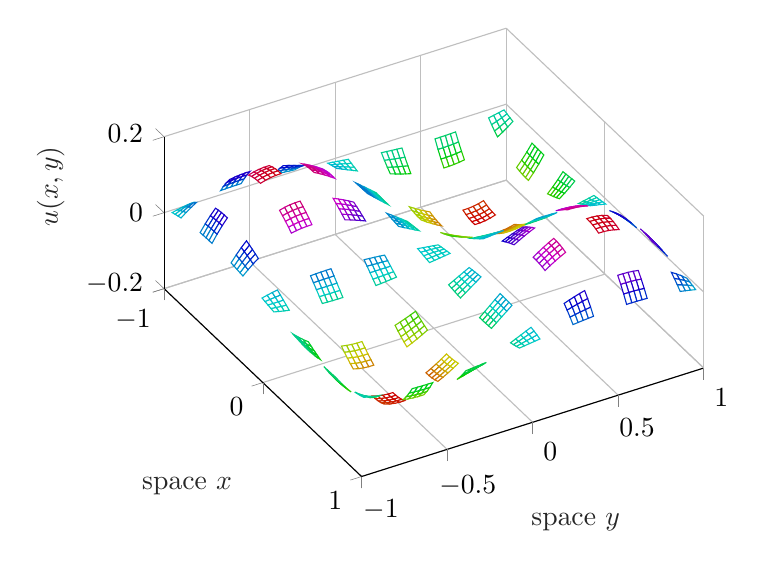
\begin{tikzpicture}

\begin{axis}[%
unbounded coords=jump,
xmin=-1,
xmax=1,
tick align=outside,
xlabel style={font=\color{white!15!black}},
xlabel={space $x$},
ymin=-1,
ymax=1,
ylabel style={font=\color{white!15!black}},
ylabel={space $y$},
zmin=-0.2,
zmax=0.2,
zlabel style={font=\color{white!15!black}},
zlabel={$u(x,y)$},
view={60}{55},
axis background/.style={fill=white},
axis x line*=bottom,
axis y line*=left,
axis z line*=left,
xmajorgrids,
ymajorgrids,
zmajorgrids,
\extraAxisOptions
]

\addplot3[%
surf,
shader=flat corner, fill=white, z buffer=sort, colormap={mymap}{[1pt] rgb(0pt)=(0.8,0,0); rgb(10pt)=(0.8,0.75,0); rgb(11pt)=(0.775,0.8,0); rgb(21pt)=(0.025,0.8,0); rgb(22pt)=(0,0.8,0.05); rgb(32pt)=(0,0.8,0.8); rgb(42pt)=(0,0.05,0.8); rgb(43pt)=(0.025,0,0.8); rgb(53pt)=(0.775,0,0.8); rgb(54pt)=(0.8,0,0.75); rgb(63pt)=(0.8,0,0.075)}, mesh/rows=42]
table[row sep=crcr, point meta=\thisrow{c}] {%
%
x	y	z	c\\
-1	-1	nan	nan\\
-1	-0.97	nan	nan\\
-1	-0.94	nan	nan\\
-1	-0.91	nan	nan\\
-1	-0.88	nan	nan\\
-1	nan	nan	nan\\
-1	-0.686666666666667	nan	nan\\
-1	-0.656666666666667	nan	nan\\
-1	-0.626666666666667	nan	nan\\
-1	-0.596666666666667	nan	nan\\
-1	-0.566666666666667	nan	nan\\
-1	nan	nan	nan\\
-1	-0.373333333333333	nan	nan\\
-1	-0.343333333333333	nan	nan\\
-1	-0.313333333333333	nan	nan\\
-1	-0.283333333333333	nan	nan\\
-1	-0.253333333333333	nan	nan\\
-1	nan	nan	nan\\
-1	-0.06	nan	nan\\
-1	-0.03	nan	nan\\
-1	0	nan	nan\\
-1	0.03	nan	nan\\
-1	0.06	nan	nan\\
-1	nan	nan	nan\\
-1	0.253333333333333	nan	nan\\
-1	0.283333333333333	nan	nan\\
-1	0.313333333333333	nan	nan\\
-1	0.343333333333333	nan	nan\\
-1	0.373333333333333	nan	nan\\
-1	nan	nan	nan\\
-1	0.566666666666666	nan	nan\\
-1	0.596666666666666	nan	nan\\
-1	0.626666666666666	nan	nan\\
-1	0.656666666666667	nan	nan\\
-1	0.686666666666667	nan	nan\\
-1	nan	nan	nan\\
-1	0.88	nan	nan\\
-1	0.91	nan	nan\\
-1	0.94	nan	nan\\
-1	0.97	nan	nan\\
-1	1	nan	nan\\
-1	nan	nan	nan\\
-0.97	-1	nan	nan\\
-0.97	-0.97	0.0032866980819905	0.0032866980819905\\
-0.97	-0.94	0.00627310293805617	0.00627310293805617\\
-0.97	-0.91	0.00896849172592129	0.00896849172592129\\
-0.97	-0.88	0.0113821479228222	0.0113821479228222\\
-0.97	nan	nan	nan\\
-0.97	-0.686666666666667	0.0208054215517705	0.0208054215517705\\
-0.97	-0.656666666666667	0.0214135981231118	0.0214135981231118\\
-0.97	-0.626666666666667	0.0218184717125587	0.0218184717125587\\
-0.97	-0.596666666666667	0.0220293324880572	0.0220293324880572\\
-0.97	-0.566666666666667	0.0220554704577758	0.0220554704577758\\
-0.97	nan	nan	nan\\
-0.97	-0.373333333333333	0.018420120589187	0.018420120589187\\
-0.97	-0.343333333333333	0.017363082652074	0.017363082652074\\
-0.97	-0.313333333333333	0.0161997641418677	0.0161997641418677\\
-0.97	-0.283333333333333	0.0149394524210268	0.0149394524210268\\
-0.97	-0.253333333333333	0.0135914348255429	0.0135914348255429\\
-0.97	nan	nan	nan\\
-0.97	-0.06	0.00342739307468705	0.00342739307468705\\
-0.97	-0.03	0.00171833932415804	0.00171833932415804\\
-0.97	0	-2.09954355971908e-17	-2.09954355971908e-17\\
-0.97	0.03	-0.00171833932415808	-0.00171833932415808\\
-0.97	0.06	-0.0034273930746871	-0.0034273930746871\\
-0.97	nan	nan	nan\\
-0.97	0.253333333333333	-0.0135914348255429	-0.0135914348255429\\
-0.97	0.283333333333333	-0.0149394524210268	-0.0149394524210268\\
-0.97	0.313333333333333	-0.0161997641418677	-0.0161997641418677\\
-0.97	0.343333333333333	-0.017363082652074	-0.017363082652074\\
-0.97	0.373333333333333	-0.018420120589187	-0.018420120589187\\
-0.97	nan	nan	nan\\
-0.97	0.566666666666666	-0.0220554704577757	-0.0220554704577757\\
-0.97	0.596666666666666	-0.0220293324880571	-0.0220293324880571\\
-0.97	0.626666666666666	-0.0218184717125586	-0.0218184717125586\\
-0.97	0.656666666666667	-0.0214135981231117	-0.0214135981231117\\
-0.97	0.686666666666667	-0.0208054215517704	-0.0208054215517704\\
-0.97	nan	nan	nan\\
-0.97	0.88	-0.0113821479228221	-0.0113821479228221\\
-0.97	0.91	-0.00896849172592122	-0.00896849172592122\\
-0.97	0.94	-0.00627310293805613	-0.00627310293805613\\
-0.97	0.97	-0.00328669808199048	-0.00328669808199048\\
-0.97	1	nan	nan\\
-0.97	nan	nan	nan\\
-0.94	-1	nan	nan\\
-0.94	-0.97	0.00627310293805617	0.00627310293805617\\
-0.94	-0.94	0.0119730545559184	0.0119730545559184\\
-0.94	-0.91	0.017117559138657	0.017117559138657\\
-0.94	-0.88	0.0217243349241318	0.0217243349241318\\
-0.94	nan	nan	nan\\
-0.94	-0.686666666666667	0.0397098769443892	0.0397098769443892\\
-0.94	-0.656666666666667	0.0408706591818508	0.0408706591818508\\
-0.94	-0.626666666666667	0.0416434104725806	0.0416434104725806\\
-0.94	-0.596666666666667	0.0420458629965131	0.0420458629965131\\
-0.94	-0.566666666666667	0.0420957484058971	0.0420957484058971\\
-0.94	nan	nan	nan\\
-0.94	-0.373333333333333	0.0351571955944552	0.0351571955944552\\
-0.94	-0.343333333333333	0.0331396994316168	0.0331396994316168\\
-0.94	-0.313333333333333	0.030919353637448	0.030919353637448\\
-0.94	-0.283333333333333	0.0285138839454287	0.0285138839454287\\
-0.94	-0.253333333333333	0.0259410162301204	0.0259410162301204\\
-0.94	nan	nan	nan\\
-0.94	-0.06	0.00654162397816271	0.00654162397816271\\
-0.94	-0.03	0.00327967340577974	0.00327967340577974\\
-0.94	0	-4.2448454403603e-17	-4.2448454403603e-17\\
-0.94	0.03	-0.00327967340577982	-0.00327967340577982\\
-0.94	0.06	-0.00654162397816279	-0.00654162397816279\\
-0.94	nan	nan	nan\\
-0.94	0.253333333333333	-0.0259410162301204	-0.0259410162301204\\
-0.94	0.283333333333333	-0.0285138839454287	-0.0285138839454287\\
-0.94	0.313333333333333	-0.030919353637448	-0.030919353637448\\
-0.94	0.343333333333333	-0.0331396994316168	-0.0331396994316168\\
-0.94	0.373333333333333	-0.0351571955944552	-0.0351571955944552\\
-0.94	nan	nan	nan\\
-0.94	0.566666666666666	-0.0420957484058969	-0.0420957484058969\\
-0.94	0.596666666666666	-0.0420458629965129	-0.0420458629965129\\
-0.94	0.626666666666666	-0.0416434104725804	-0.0416434104725804\\
-0.94	0.656666666666667	-0.0408706591818506	-0.0408706591818506\\
-0.94	0.686666666666667	-0.039709876944389	-0.039709876944389\\
-0.94	nan	nan	nan\\
-0.94	0.88	-0.0217243349241317	-0.0217243349241317\\
-0.94	0.91	-0.0171175591386569	-0.0171175591386569\\
-0.94	0.94	-0.0119730545559183	-0.0119730545559183\\
-0.94	0.97	-0.00627310293805613	-0.00627310293805613\\
-0.94	1	nan	nan\\
-0.94	nan	nan	nan\\
-0.91	-1	nan	nan\\
-0.91	-0.97	0.00896849172592129	0.00896849172592129\\
-0.91	-0.94	0.017117559138657	0.017117559138657\\
-0.91	-0.91	0.0244725072080051	0.0244725072080051\\
-0.91	-0.88	0.031058662907789	0.031058662907789\\
-0.91	nan	nan	nan\\
-0.91	-0.686666666666667	0.0567720580718161	0.0567720580718161\\
-0.91	-0.656666666666667	0.0584315946978227	0.0584315946978227\\
-0.91	-0.626666666666667	0.0595363724912943	0.0595363724912943\\
-0.91	-0.596666666666667	0.0601117454543235	0.0601117454543235\\
-0.91	-0.566666666666667	0.0601830662918983	0.0601830662918983\\
-0.91	nan	nan	nan\\
-0.91	-0.373333333333333	0.0502632170306453	0.0502632170306453\\
-0.91	-0.343333333333333	0.0473788608293143	0.0473788608293143\\
-0.91	-0.313333333333333	0.0442044979741044	0.0442044979741044\\
-0.91	-0.283333333333333	0.0407654685500945	0.0407654685500945\\
-0.91	-0.253333333333333	0.0370871132583797	0.0370871132583797\\
-0.91	nan	nan	nan\\
-0.91	-0.06	0.00935236849266306	0.00935236849266306\\
-0.91	-0.03	0.00468885378618707	0.00468885378618707\\
-0.91	0	-6.51668193805004e-17	-6.51668193805004e-17\\
-0.91	0.03	-0.00468885378618721	-0.00468885378618721\\
-0.91	0.06	-0.00935236849266319	-0.00935236849266319\\
-0.91	nan	nan	nan\\
-0.91	0.253333333333333	-0.0370871132583797	-0.0370871132583797\\
-0.91	0.283333333333333	-0.0407654685500946	-0.0407654685500946\\
-0.91	0.313333333333333	-0.0442044979741044	-0.0442044979741044\\
-0.91	0.343333333333333	-0.0473788608293142	-0.0473788608293142\\
-0.91	0.373333333333333	-0.0502632170306452	-0.0502632170306452\\
-0.91	nan	nan	nan\\
-0.91	0.566666666666666	-0.060183066291898	-0.060183066291898\\
-0.91	0.596666666666666	-0.0601117454543232	-0.0601117454543232\\
-0.91	0.626666666666666	-0.059536372491294	-0.059536372491294\\
-0.91	0.656666666666667	-0.0584315946978224	-0.0584315946978224\\
-0.91	0.686666666666667	-0.0567720580718158	-0.0567720580718158\\
-0.91	nan	nan	nan\\
-0.91	0.88	-0.0310586629077887	-0.0310586629077887\\
-0.91	0.91	-0.0244725072080049	-0.0244725072080049\\
-0.91	0.94	-0.0171175591386569	-0.0171175591386569\\
-0.91	0.97	-0.00896849172592122	-0.00896849172592122\\
-0.91	1	nan	nan\\
-0.91	nan	nan	nan\\
-0.88	-1	nan	nan\\
-0.88	-0.97	0.0113821479228222	0.0113821479228222\\
-0.88	-0.94	0.0217243349241318	0.0217243349241318\\
-0.88	-0.91	0.031058662907789	0.031058662907789\\
-0.88	-0.88	0.039417247761044	0.039417247761044\\
-0.88	nan	nan	nan\\
-0.88	-0.686666666666667	0.0720506741814657	0.0720506741814657\\
-0.88	-0.656666666666667	0.0741568390643742	0.0741568390643742\\
-0.88	-0.626666666666667	0.0755589357981557	0.0755589357981557\\
-0.88	-0.596666666666667	0.0762891532793162	0.0762891532793162\\
-0.88	-0.566666666666667	0.076379679837679	0.076379679837679\\
-0.88	nan	nan	nan\\
-0.88	-0.373333333333333	0.0637901988666771	0.0637901988666771\\
-0.88	-0.343333333333333	0.0601295960853067	0.0601295960853067\\
-0.88	-0.313333333333333	0.0561009456383716	0.0561009456383716\\
-0.88	-0.283333333333333	0.0517363999067925	0.0517363999067925\\
-0.88	-0.253333333333333	0.047068110184786	0.047068110184786\\
-0.88	nan	nan	nan\\
-0.88	-0.06	0.0118693056674313	0.0118693056674313\\
-0.88	-0.03	0.00595073542783294	0.00595073542783294\\
-0.88	0	-8.56510695869088e-17	-8.56510695869088e-17\\
-0.88	0.03	-0.00595073542783312	-0.00595073542783312\\
-0.88	0.06	-0.0118693056674315	-0.0118693056674315\\
-0.88	nan	nan	nan\\
-0.88	0.253333333333333	-0.047068110184786	-0.047068110184786\\
-0.88	0.283333333333333	-0.0517363999067925	-0.0517363999067925\\
-0.88	0.313333333333333	-0.0561009456383716	-0.0561009456383716\\
-0.88	0.343333333333333	-0.0601295960853066	-0.0601295960853066\\
-0.88	0.373333333333333	-0.063790198866677	-0.063790198866677\\
-0.88	nan	nan	nan\\
-0.88	0.566666666666666	-0.0763796798376787	-0.0763796798376787\\
-0.88	0.596666666666666	-0.0762891532793158	-0.0762891532793158\\
-0.88	0.626666666666666	-0.0755589357981553	-0.0755589357981553\\
-0.88	0.656666666666667	-0.0741568390643738	-0.0741568390643738\\
-0.88	0.686666666666667	-0.0720506741814653	-0.0720506741814653\\
-0.88	nan	nan	nan\\
-0.88	0.88	-0.0394172477610437	-0.0394172477610437\\
-0.88	0.91	-0.0310586629077887	-0.0310586629077887\\
-0.88	0.94	-0.0217243349241317	-0.0217243349241317\\
-0.88	0.97	-0.0113821479228221	-0.0113821479228221\\
-0.88	1	nan	nan\\
-0.88	nan	nan	nan\\
nan	-1	nan	nan\\
nan	-0.97	nan	nan\\
nan	-0.94	nan	nan\\
nan	-0.91	nan	nan\\
nan	-0.88	nan	nan\\
nan	nan	nan	nan\\
nan	-0.686666666666667	nan	nan\\
nan	-0.656666666666667	nan	nan\\
nan	-0.626666666666667	nan	nan\\
nan	-0.596666666666667	nan	nan\\
nan	-0.566666666666667	nan	nan\\
nan	nan	nan	nan\\
nan	-0.373333333333333	nan	nan\\
nan	-0.343333333333333	nan	nan\\
nan	-0.313333333333333	nan	nan\\
nan	-0.283333333333333	nan	nan\\
nan	-0.253333333333333	nan	nan\\
nan	nan	nan	nan\\
nan	-0.06	nan	nan\\
nan	-0.03	nan	nan\\
nan	0	nan	nan\\
nan	0.03	nan	nan\\
nan	0.06	nan	nan\\
nan	nan	nan	nan\\
nan	0.253333333333333	nan	nan\\
nan	0.283333333333333	nan	nan\\
nan	0.313333333333333	nan	nan\\
nan	0.343333333333333	nan	nan\\
nan	0.373333333333333	nan	nan\\
nan	nan	nan	nan\\
nan	0.566666666666666	nan	nan\\
nan	0.596666666666666	nan	nan\\
nan	0.626666666666666	nan	nan\\
nan	0.656666666666667	nan	nan\\
nan	0.686666666666667	nan	nan\\
nan	nan	nan	nan\\
nan	0.88	nan	nan\\
nan	0.91	nan	nan\\
nan	0.94	nan	nan\\
nan	0.97	nan	nan\\
nan	1	nan	nan\\
nan	nan	nan	nan\\
-0.686666666666667	-1	nan	nan\\
-0.686666666666667	-0.97	0.0208054215517705	0.0208054215517705\\
-0.686666666666667	-0.94	0.0397098769443892	0.0397098769443892\\
-0.686666666666667	-0.91	0.0567720580718161	0.0567720580718161\\
-0.686666666666667	-0.88	0.0720506741814657	0.0720506741814657\\
-0.686666666666667	nan	nan	nan\\
-0.686666666666667	-0.686666666666667	0.131696536183093	0.131696536183093\\
-0.686666666666667	-0.656666666666667	0.135545560874128	0.135545560874128\\
-0.686666666666667	-0.626666666666667	0.138107629672581	0.138107629672581\\
-0.686666666666667	-0.596666666666667	0.139441591069571	0.139441591069571\\
-0.686666666666667	-0.566666666666667	0.139606294253937	0.139606294253937\\
-0.686666666666667	nan	nan	nan\\
-0.686666666666667	-0.373333333333333	0.116591827484176	0.116591827484176\\
-0.686666666666667	-0.343333333333333	0.109900706198424	0.109900706198424\\
-0.686666666666667	-0.313333333333333	0.102536991393087	0.102536991393087\\
-0.686666666666667	-0.283333333333333	0.0945594625394479	0.0945594625394479\\
-0.686666666666667	-0.253333333333333	0.0860268928632561	0.0860268928632561\\
-0.686666666666667	nan	nan	nan\\
-0.686666666666667	-0.06	0.0216935927204082	0.0216935927204082\\
-0.686666666666667	-0.03	0.0108761788399837	0.0108761788399837\\
-0.686666666666667	0	-7.42491156260814e-17	-7.42491156260814e-17\\
-0.686666666666667	0.03	-0.0108761788399839	-0.0108761788399839\\
-0.686666666666667	0.06	-0.0216935927204083	-0.0216935927204083\\
-0.686666666666667	nan	nan	nan\\
-0.686666666666667	0.253333333333333	-0.086026892863256	-0.086026892863256\\
-0.686666666666667	0.283333333333333	-0.0945594625394479	-0.0945594625394479\\
-0.686666666666667	0.313333333333333	-0.102536991393087	-0.102536991393087\\
-0.686666666666667	0.343333333333333	-0.109900706198423	-0.109900706198423\\
-0.686666666666667	0.373333333333333	-0.116591827484176	-0.116591827484176\\
-0.686666666666667	nan	nan	nan\\
-0.686666666666667	0.566666666666666	-0.139606294253936	-0.139606294253936\\
-0.686666666666667	0.596666666666666	-0.13944159106957	-0.13944159106957\\
-0.686666666666667	0.626666666666666	-0.138107629672581	-0.138107629672581\\
-0.686666666666667	0.656666666666667	-0.135545560874127	-0.135545560874127\\
-0.686666666666667	0.686666666666667	-0.131696536183092	-0.131696536183092\\
-0.686666666666667	nan	nan	nan\\
-0.686666666666667	0.88	-0.0720506741814651	-0.0720506741814651\\
-0.686666666666667	0.91	-0.0567720580718157	-0.0567720580718157\\
-0.686666666666667	0.94	-0.0397098769443889	-0.0397098769443889\\
-0.686666666666667	0.97	-0.0208054215517703	-0.0208054215517703\\
-0.686666666666667	1	nan	nan\\
-0.686666666666667	nan	nan	nan\\
-0.656666666666667	-1	nan	nan\\
-0.656666666666667	-0.97	0.0214135981231118	0.0214135981231118\\
-0.656666666666667	-0.94	0.0408706591818508	0.0408706591818508\\
-0.656666666666667	-0.91	0.0584315946978227	0.0584315946978227\\
-0.656666666666667	-0.88	0.0741568390643742	0.0741568390643742\\
-0.656666666666667	nan	nan	nan\\
-0.656666666666667	-0.686666666666667	0.135545560874128	0.135545560874128\\
-0.656666666666667	-0.656666666666667	0.139506973113684	0.139506973113684\\
-0.656666666666667	-0.626666666666667	0.142143814509802	0.142143814509802\\
-0.656666666666667	-0.596666666666667	0.143516651559025	0.143516651559025\\
-0.656666666666667	-0.566666666666667	0.143686051930182	0.143686051930182\\
-0.656666666666667	nan	nan	nan\\
-0.656666666666667	-0.373333333333333	0.119998502729756	0.119998502729756\\
-0.656666666666667	-0.343333333333333	0.113111801758318	0.113111801758318\\
-0.656666666666667	-0.313333333333333	0.105532867898494	0.105532867898494\\
-0.656666666666667	-0.283333333333333	0.0973222023005611	0.0973222023005611\\
-0.656666666666667	-0.253333333333333	0.0885402995245026	0.0885402995245026\\
-0.656666666666667	nan	nan	nan\\
-0.656666666666667	-0.06	0.0223273946315712	0.0223273946315712\\
-0.656666666666667	-0.03	0.0111939354530749	0.0111939354530749\\
-0.656666666666667	0	-6.60130511774821e-17	-6.60130511774821e-17\\
-0.656666666666667	0.03	-0.0111939354530751	-0.0111939354530751\\
-0.656666666666667	0.06	-0.0223273946315714	-0.0223273946315714\\
-0.656666666666667	nan	nan	nan\\
-0.656666666666667	0.253333333333333	-0.0885402995245024	-0.0885402995245024\\
-0.656666666666667	0.283333333333333	-0.0973222023005609	-0.0973222023005609\\
-0.656666666666667	0.313333333333333	-0.105532867898494	-0.105532867898494\\
-0.656666666666667	0.343333333333333	-0.113111801758318	-0.113111801758318\\
-0.656666666666667	0.373333333333333	-0.119998502729755	-0.119998502729755\\
-0.656666666666667	nan	nan	nan\\
-0.656666666666667	0.566666666666666	-0.143686051930181	-0.143686051930181\\
-0.656666666666667	0.596666666666666	-0.143516651559025	-0.143516651559025\\
-0.656666666666667	0.626666666666666	-0.142143814509801	-0.142143814509801\\
-0.656666666666667	0.656666666666667	-0.139506973113683	-0.139506973113683\\
-0.656666666666667	0.686666666666667	-0.135545560874127	-0.135545560874127\\
-0.656666666666667	nan	nan	nan\\
-0.656666666666667	0.88	-0.0741568390643736	-0.0741568390643736\\
-0.656666666666667	0.91	-0.0584315946978222	-0.0584315946978222\\
-0.656666666666667	0.94	-0.0408706591818505	-0.0408706591818505\\
-0.656666666666667	0.97	-0.0214135981231117	-0.0214135981231117\\
-0.656666666666667	1	nan	nan\\
-0.656666666666667	nan	nan	nan\\
-0.626666666666667	-1	nan	nan\\
-0.626666666666667	-0.97	0.0218184717125587	0.0218184717125587\\
-0.626666666666667	-0.94	0.0416434104725806	0.0416434104725806\\
-0.626666666666667	-0.91	0.0595363724912943	0.0595363724912943\\
-0.626666666666667	-0.88	0.0755589357981557	0.0755589357981557\\
-0.626666666666667	nan	nan	nan\\
-0.626666666666667	-0.686666666666667	0.138107629672581	0.138107629672581\\
-0.626666666666667	-0.656666666666667	0.142143814509802	0.142143814509802\\
-0.626666666666667	-0.626666666666667	0.144830385681669	0.144830385681669\\
-0.626666666666667	-0.596666666666667	0.146229056810971	0.146229056810971\\
-0.626666666666667	-0.566666666666667	0.146401542218275	0.146401542218275\\
-0.626666666666667	nan	nan	nan\\
-0.626666666666667	-0.373333333333333	0.122265792837812	0.122265792837812\\
-0.626666666666667	-0.343333333333333	0.115248896546735	0.115248896546735\\
-0.626666666666667	-0.313333333333333	0.107526703671996	0.107526703671996\\
-0.626666666666667	-0.283333333333333	0.0991608603722466	0.0991608603722466\\
-0.626666666666667	-0.253333333333333	0.0902130058385126	0.0902130058385126\\
-0.626666666666667	nan	nan	nan\\
-0.626666666666667	-0.06	0.0227491945160275	0.0227491945160275\\
-0.626666666666667	-0.03	0.0114054048495779	0.0114054048495779\\
-0.626666666666667	0	-5.28524410582676e-17	-5.28524410582676e-17\\
-0.626666666666667	0.03	-0.011405404849578	-0.011405404849578\\
-0.626666666666667	0.06	-0.0227491945160277	-0.0227491945160277\\
-0.626666666666667	nan	nan	nan\\
-0.626666666666667	0.253333333333333	-0.0902130058385125	-0.0902130058385125\\
-0.626666666666667	0.283333333333333	-0.0991608603722465	-0.0991608603722465\\
-0.626666666666667	0.313333333333333	-0.107526703671996	-0.107526703671996\\
-0.626666666666667	0.343333333333333	-0.115248896546734	-0.115248896546734\\
-0.626666666666667	0.373333333333333	-0.122265792837811	-0.122265792837811\\
-0.626666666666667	nan	nan	nan\\
-0.626666666666667	0.566666666666666	-0.146401542218275	-0.146401542218275\\
-0.626666666666667	0.596666666666666	-0.14622905681097	-0.14622905681097\\
-0.626666666666667	0.626666666666666	-0.144830385681669	-0.144830385681669\\
-0.626666666666667	0.656666666666667	-0.142143814509801	-0.142143814509801\\
-0.626666666666667	0.686666666666667	-0.13810762967258	-0.13810762967258\\
-0.626666666666667	nan	nan	nan\\
-0.626666666666667	0.88	-0.0755589357981551	-0.0755589357981551\\
-0.626666666666667	0.91	-0.0595363724912938	-0.0595363724912938\\
-0.626666666666667	0.94	-0.0416434104725802	-0.0416434104725802\\
-0.626666666666667	0.97	-0.0218184717125585	-0.0218184717125585\\
-0.626666666666667	1	nan	nan\\
-0.626666666666667	nan	nan	nan\\
-0.596666666666667	-1	nan	nan\\
-0.596666666666667	-0.97	0.0220293324880572	0.0220293324880572\\
-0.596666666666667	-0.94	0.0420458629965131	0.0420458629965131\\
-0.596666666666667	-0.91	0.0601117454543235	0.0601117454543235\\
-0.596666666666667	-0.88	0.0762891532793162	0.0762891532793162\\
-0.596666666666667	nan	nan	nan\\
-0.596666666666667	-0.686666666666667	0.139441591069571	0.139441591069571\\
-0.596666666666667	-0.656666666666667	0.143516651559025	0.143516651559025\\
-0.596666666666667	-0.626666666666667	0.146229056810971	0.146229056810971\\
-0.596666666666667	-0.596666666666667	0.147641118123951	0.147641118123951\\
-0.596666666666667	-0.566666666666667	0.147815148522	0.147815148522\\
-0.596666666666667	nan	nan	nan\\
-0.596666666666667	-0.373333333333333	0.123445799088296	0.123445799088296\\
-0.596666666666667	-0.343333333333333	0.11636110318044	0.11636110318044\\
-0.596666666666667	-0.313333333333333	0.10856431978342	0.10856431978342\\
-0.596666666666667	-0.283333333333333	0.100117692356374	0.100117692356374\\
-0.596666666666667	-0.253333333333333	0.091083456149039	0.091083456149039\\
-0.596666666666667	nan	nan	nan\\
-0.596666666666667	-0.06	0.0229686873776171	0.0229686873776171\\
-0.596666666666667	-0.03	0.0115154466587653	0.0115154466587653\\
-0.596666666666667	0	-3.72633113786586e-17	-3.72633113786586e-17\\
-0.596666666666667	0.03	-0.0115154466587653	-0.0115154466587653\\
-0.596666666666667	0.06	-0.0229686873776172	-0.0229686873776172\\
-0.596666666666667	nan	nan	nan\\
-0.596666666666667	0.253333333333333	-0.0910834561490389	-0.0910834561490389\\
-0.596666666666667	0.283333333333333	-0.100117692356374	-0.100117692356374\\
-0.596666666666667	0.313333333333333	-0.10856431978342	-0.10856431978342\\
-0.596666666666667	0.343333333333333	-0.11636110318044	-0.11636110318044\\
-0.596666666666667	0.373333333333333	-0.123445799088295	-0.123445799088295\\
-0.596666666666667	nan	nan	nan\\
-0.596666666666667	0.566666666666666	-0.147815148521999	-0.147815148521999\\
-0.596666666666667	0.596666666666666	-0.14764111812395	-0.14764111812395\\
-0.596666666666667	0.626666666666666	-0.14622905681097	-0.14622905681097\\
-0.596666666666667	0.656666666666667	-0.143516651559025	-0.143516651559025\\
-0.596666666666667	0.686666666666667	-0.13944159106957	-0.13944159106957\\
-0.596666666666667	nan	nan	nan\\
-0.596666666666667	0.88	-0.0762891532793155	-0.0762891532793155\\
-0.596666666666667	0.91	-0.060111745454323	-0.060111745454323\\
-0.596666666666667	0.94	-0.0420458629965128	-0.0420458629965128\\
-0.596666666666667	0.97	-0.022029332488057	-0.022029332488057\\
-0.596666666666667	1	nan	nan\\
-0.596666666666667	nan	nan	nan\\
-0.566666666666667	-1	nan	nan\\
-0.566666666666667	-0.97	0.0220554704577758	0.0220554704577758\\
-0.566666666666667	-0.94	0.0420957484058971	0.0420957484058971\\
-0.566666666666667	-0.91	0.0601830662918983	0.0601830662918983\\
-0.566666666666667	-0.88	0.076379679837679	0.076379679837679\\
-0.566666666666667	nan	nan	nan\\
-0.566666666666667	-0.686666666666667	0.139606294253937	0.139606294253937\\
-0.566666666666667	-0.656666666666667	0.143686051930182	0.143686051930182\\
-0.566666666666667	-0.626666666666667	0.146401542218275	0.146401542218275\\
-0.566666666666667	-0.596666666666667	0.147815148522	0.147815148522\\
-0.566666666666667	-0.566666666666667	0.147989256363696	0.147989256363696\\
-0.566666666666667	nan	nan	nan\\
-0.566666666666667	-0.373333333333333	0.123590625904809	0.123590625904809\\
-0.566666666666667	-0.343333333333333	0.116497537504207	0.116497537504207\\
-0.566666666666667	-0.313333333333333	0.108691540887749	0.108691540887749\\
-0.566666666666667	-0.283333333333333	0.100234956857915	0.100234956857915\\
-0.566666666666667	-0.253333333333333	0.0911900977186031	0.0911900977186031\\
-0.566666666666667	nan	nan	nan\\
-0.566666666666667	-0.06	0.0229955689299039	0.0229955689299039\\
-0.566666666666667	-0.03	0.0115289209343136	0.0115289209343136\\
-0.566666666666667	0	-2.36831359439194e-17	-2.36831359439194e-17\\
-0.566666666666667	0.03	-0.0115289209343137	-0.0115289209343137\\
-0.566666666666667	0.06	-0.0229955689299039	-0.0229955689299039\\
-0.566666666666667	nan	nan	nan\\
-0.566666666666667	0.253333333333333	-0.0911900977186029	-0.0911900977186029\\
-0.566666666666667	0.283333333333333	-0.100234956857914	-0.100234956857914\\
-0.566666666666667	0.313333333333333	-0.108691540887749	-0.108691540887749\\
-0.566666666666667	0.343333333333333	-0.116497537504207	-0.116497537504207\\
-0.566666666666667	0.373333333333333	-0.123590625904809	-0.123590625904809\\
-0.566666666666667	nan	nan	nan\\
-0.566666666666667	0.566666666666666	-0.147989256363695	-0.147989256363695\\
-0.566666666666667	0.596666666666666	-0.147815148521999	-0.147815148521999\\
-0.566666666666667	0.626666666666666	-0.146401542218274	-0.146401542218274\\
-0.566666666666667	0.656666666666667	-0.143686051930181	-0.143686051930181\\
-0.566666666666667	0.686666666666667	-0.139606294253936	-0.139606294253936\\
-0.566666666666667	nan	nan	nan\\
-0.566666666666667	0.88	-0.0763796798376784	-0.0763796798376784\\
-0.566666666666667	0.91	-0.0601830662918978	-0.0601830662918978\\
-0.566666666666667	0.94	-0.0420957484058968	-0.0420957484058968\\
-0.566666666666667	0.97	-0.0220554704577756	-0.0220554704577756\\
-0.566666666666667	1	nan	nan\\
-0.566666666666667	nan	nan	nan\\
nan	-1	nan	nan\\
nan	-0.97	nan	nan\\
nan	-0.94	nan	nan\\
nan	-0.91	nan	nan\\
nan	-0.88	nan	nan\\
nan	nan	nan	nan\\
nan	-0.686666666666667	nan	nan\\
nan	-0.656666666666667	nan	nan\\
nan	-0.626666666666667	nan	nan\\
nan	-0.596666666666667	nan	nan\\
nan	-0.566666666666667	nan	nan\\
nan	nan	nan	nan\\
nan	-0.373333333333333	nan	nan\\
nan	-0.343333333333333	nan	nan\\
nan	-0.313333333333333	nan	nan\\
nan	-0.283333333333333	nan	nan\\
nan	-0.253333333333333	nan	nan\\
nan	nan	nan	nan\\
nan	-0.06	nan	nan\\
nan	-0.03	nan	nan\\
nan	0	nan	nan\\
nan	0.03	nan	nan\\
nan	0.06	nan	nan\\
nan	nan	nan	nan\\
nan	0.253333333333333	nan	nan\\
nan	0.283333333333333	nan	nan\\
nan	0.313333333333333	nan	nan\\
nan	0.343333333333333	nan	nan\\
nan	0.373333333333333	nan	nan\\
nan	nan	nan	nan\\
nan	0.566666666666666	nan	nan\\
nan	0.596666666666666	nan	nan\\
nan	0.626666666666666	nan	nan\\
nan	0.656666666666667	nan	nan\\
nan	0.686666666666667	nan	nan\\
nan	nan	nan	nan\\
nan	0.88	nan	nan\\
nan	0.91	nan	nan\\
nan	0.94	nan	nan\\
nan	0.97	nan	nan\\
nan	1	nan	nan\\
nan	nan	nan	nan\\
-0.373333333333333	-1	nan	nan\\
-0.373333333333333	-0.97	0.018420120589187	0.018420120589187\\
-0.373333333333333	-0.94	0.0351571955944552	0.0351571955944552\\
-0.373333333333333	-0.91	0.0502632170306453	0.0502632170306453\\
-0.373333333333333	-0.88	0.0637901988666771	0.0637901988666771\\
-0.373333333333333	nan	nan	nan\\
-0.373333333333333	-0.686666666666667	0.116591827484176	0.116591827484176\\
-0.373333333333333	-0.656666666666667	0.119998502729756	0.119998502729756\\
-0.373333333333333	-0.626666666666667	0.122265792837812	0.122265792837812\\
-0.373333333333333	-0.596666666666667	0.123445799088296	0.123445799088296\\
-0.373333333333333	-0.566666666666667	0.123590625904809	0.123590625904809\\
-0.373333333333333	nan	nan	nan\\
-0.373333333333333	-0.373333333333333	0.103211911138823	0.103211911138823\\
-0.373333333333333	-0.343333333333333	0.0972880235434752	0.0972880235434752\\
-0.373333333333333	-0.313333333333333	0.0907688503109018	0.0907688503109018\\
-0.373333333333333	-0.283333333333333	0.0837064508198778	0.0837064508198778\\
-0.373333333333333	-0.253333333333333	0.0761528749748297	0.0761528749748297\\
-0.373333333333333	nan	nan	nan\\
-0.373333333333333	-0.06	0.0192035573251247	0.0192035573251247\\
-0.373333333333333	-0.03	0.00962776980008805	0.00962776980008805\\
-0.373333333333333	0	6.42966483119013e-17	6.42966483119013e-17\\
-0.373333333333333	0.03	-0.00962776980008792	-0.00962776980008792\\
-0.373333333333333	0.06	-0.0192035573251245	-0.0192035573251245\\
-0.373333333333333	nan	nan	nan\\
-0.373333333333333	0.253333333333333	-0.0761528749748294	-0.0761528749748294\\
-0.373333333333333	0.283333333333333	-0.0837064508198774	-0.0837064508198774\\
-0.373333333333333	0.313333333333333	-0.0907688503109013	-0.0907688503109013\\
-0.373333333333333	0.343333333333333	-0.0972880235434747	-0.0972880235434747\\
-0.373333333333333	0.373333333333333	-0.103211911138822	-0.103211911138822\\
-0.373333333333333	nan	nan	nan\\
-0.373333333333333	0.566666666666666	-0.123590625904809	-0.123590625904809\\
-0.373333333333333	0.596666666666666	-0.123445799088295	-0.123445799088295\\
-0.373333333333333	0.626666666666666	-0.122265792837811	-0.122265792837811\\
-0.373333333333333	0.656666666666667	-0.119998502729755	-0.119998502729755\\
-0.373333333333333	0.686666666666667	-0.116591827484175	-0.116591827484175\\
-0.373333333333333	nan	nan	nan\\
-0.373333333333333	0.88	-0.0637901988666766	-0.0637901988666766\\
-0.373333333333333	0.91	-0.0502632170306449	-0.0502632170306449\\
-0.373333333333333	0.94	-0.0351571955944549	-0.0351571955944549\\
-0.373333333333333	0.97	-0.0184201205891869	-0.0184201205891869\\
-0.373333333333333	1	nan	nan\\
-0.373333333333333	nan	nan	nan\\
-0.343333333333333	-1	nan	nan\\
-0.343333333333333	-0.97	0.017363082652074	0.017363082652074\\
-0.343333333333333	-0.94	0.0331396994316168	0.0331396994316168\\
-0.343333333333333	-0.91	0.0473788608293143	0.0473788608293143\\
-0.343333333333333	-0.88	0.0601295960853067	0.0601295960853067\\
-0.343333333333333	nan	nan	nan\\
-0.343333333333333	-0.686666666666667	0.109900706198424	0.109900706198424\\
-0.343333333333333	-0.656666666666667	0.113111801758318	0.113111801758318\\
-0.343333333333333	-0.626666666666667	0.115248896546735	0.115248896546735\\
-0.343333333333333	-0.596666666666667	0.11636110318044	0.11636110318044\\
-0.343333333333333	-0.566666666666667	0.116497537504207	0.116497537504207\\
-0.343333333333333	nan	nan	nan\\
-0.343333333333333	-0.373333333333333	0.0972880235434752	0.0972880235434752\\
-0.343333333333333	-0.343333333333333	0.0917040871913489	0.0917040871913489\\
-0.343333333333333	-0.313333333333333	0.0855590426731921	0.0855590426731921\\
-0.343333333333333	-0.283333333333333	0.0789019628111265	0.0789019628111265\\
-0.343333333333333	-0.253333333333333	0.0717819109116259	0.0717819109116259\\
-0.343333333333333	nan	nan	nan\\
-0.343333333333333	-0.06	0.0181013193947797	0.0181013193947797\\
-0.343333333333333	-0.03	0.00907515779192914	0.00907515779192914\\
-0.343333333333333	0	7.55992821413424e-17	7.55992821413424e-17\\
-0.343333333333333	0.03	-0.00907515779192898	-0.00907515779192898\\
-0.343333333333333	0.06	-0.0181013193947796	-0.0181013193947796\\
-0.343333333333333	nan	nan	nan\\
-0.343333333333333	0.253333333333333	-0.0717819109116256	-0.0717819109116256\\
-0.343333333333333	0.283333333333333	-0.0789019628111261	-0.0789019628111261\\
-0.343333333333333	0.313333333333333	-0.0855590426731916	-0.0855590426731916\\
-0.343333333333333	0.343333333333333	-0.0917040871913484	-0.0917040871913484\\
-0.343333333333333	0.373333333333333	-0.0972880235434746	-0.0972880235434746\\
-0.343333333333333	nan	nan	nan\\
-0.343333333333333	0.566666666666666	-0.116497537504206	-0.116497537504206\\
-0.343333333333333	0.596666666666666	-0.11636110318044	-0.11636110318044\\
-0.343333333333333	0.626666666666666	-0.115248896546734	-0.115248896546734\\
-0.343333333333333	0.656666666666667	-0.113111801758317	-0.113111801758317\\
-0.343333333333333	0.686666666666667	-0.109900706198423	-0.109900706198423\\
-0.343333333333333	nan	nan	nan\\
-0.343333333333333	0.88	-0.0601295960853062	-0.0601295960853062\\
-0.343333333333333	0.91	-0.0473788608293139	-0.0473788608293139\\
-0.343333333333333	0.94	-0.0331396994316165	-0.0331396994316165\\
-0.343333333333333	0.97	-0.0173630826520739	-0.0173630826520739\\
-0.343333333333333	1	nan	nan\\
-0.343333333333333	nan	nan	nan\\
-0.313333333333333	-1	nan	nan\\
-0.313333333333333	-0.97	0.0161997641418677	0.0161997641418677\\
-0.313333333333333	-0.94	0.030919353637448	0.030919353637448\\
-0.313333333333333	-0.91	0.0442044979741044	0.0442044979741044\\
-0.313333333333333	-0.88	0.0561009456383717	0.0561009456383717\\
-0.313333333333333	nan	nan	nan\\
-0.313333333333333	-0.686666666666667	0.102536991393087	0.102536991393087\\
-0.313333333333333	-0.656666666666667	0.105532867898494	0.105532867898494\\
-0.313333333333333	-0.626666666666667	0.107526703671996	0.107526703671996\\
-0.313333333333333	-0.596666666666667	0.10856431978342	0.10856431978342\\
-0.313333333333333	-0.566666666666667	0.108691540887749	0.108691540887749\\
-0.313333333333333	nan	nan	nan\\
-0.313333333333333	-0.373333333333333	0.0907688503109018	0.0907688503109018\\
-0.313333333333333	-0.343333333333333	0.0855590426731921	0.0855590426731921\\
-0.313333333333333	-0.313333333333333	0.0798257344827885	0.0798257344827885\\
-0.313333333333333	-0.283333333333333	0.0736147126517809	0.0736147126517809\\
-0.313333333333333	-0.253333333333333	0.0669717548079212	0.0669717548079212\\
-0.313333333333333	nan	nan	nan\\
-0.313333333333333	-0.06	0.0168883314375885	0.0168883314375885\\
-0.313333333333333	-0.03	0.00846702059608703	0.00846702059608703\\
-0.313333333333333	0	8.30702876848249e-17	8.30702876848249e-17\\
-0.313333333333333	0.03	-0.00846702059608686	-0.00846702059608686\\
-0.313333333333333	0.06	-0.0168883314375883	-0.0168883314375883\\
-0.313333333333333	nan	nan	nan\\
-0.313333333333333	0.253333333333333	-0.0669717548079208	-0.0669717548079208\\
-0.313333333333333	0.283333333333333	-0.0736147126517805	-0.0736147126517805\\
-0.313333333333333	0.313333333333333	-0.0798257344827881	-0.0798257344827881\\
-0.313333333333333	0.343333333333333	-0.0855590426731916	-0.0855590426731916\\
-0.313333333333333	0.373333333333333	-0.0907688503109012	-0.0907688503109012\\
-0.313333333333333	nan	nan	nan\\
-0.313333333333333	0.566666666666666	-0.108691540887749	-0.108691540887749\\
-0.313333333333333	0.596666666666666	-0.10856431978342	-0.10856431978342\\
-0.313333333333333	0.626666666666666	-0.107526703671996	-0.107526703671996\\
-0.313333333333333	0.656666666666667	-0.105532867898494	-0.105532867898494\\
-0.313333333333333	0.686666666666667	-0.102536991393086	-0.102536991393086\\
-0.313333333333333	nan	nan	nan\\
-0.313333333333333	0.88	-0.0561009456383712	-0.0561009456383712\\
-0.313333333333333	0.91	-0.044204497974104	-0.044204497974104\\
-0.313333333333333	0.94	-0.0309193536374477	-0.0309193536374477\\
-0.313333333333333	0.97	-0.0161997641418675	-0.0161997641418675\\
-0.313333333333333	1	nan	nan\\
-0.313333333333333	nan	nan	nan\\
-0.283333333333333	-1	nan	nan\\
-0.283333333333333	-0.97	0.0149394524210268	0.0149394524210268\\
-0.283333333333333	-0.94	0.0285138839454287	0.0285138839454287\\
-0.283333333333333	-0.91	0.0407654685500946	0.0407654685500946\\
-0.283333333333333	-0.88	0.0517363999067925	0.0517363999067925\\
-0.283333333333333	nan	nan	nan\\
-0.283333333333333	-0.686666666666667	0.094559462539448	0.094559462539448\\
-0.283333333333333	-0.656666666666667	0.0973222023005611	0.0973222023005611\\
-0.283333333333333	-0.626666666666667	0.0991608603722467	0.0991608603722467\\
-0.283333333333333	-0.596666666666667	0.100117692356374	0.100117692356374\\
-0.283333333333333	-0.566666666666667	0.100234956857915	0.100234956857915\\
-0.283333333333333	nan	nan	nan\\
-0.283333333333333	-0.373333333333333	0.0837064508198778	0.0837064508198778\\
-0.283333333333333	-0.343333333333333	0.0789019628111265	0.0789019628111265\\
-0.283333333333333	-0.313333333333333	0.0736147126517809	0.0736147126517809\\
-0.283333333333333	-0.283333333333333	0.0678869266358654	0.0678869266358654\\
-0.283333333333333	-0.253333333333333	0.0617608226769526	0.0617608226769526\\
-0.283333333333333	nan	nan	nan\\
-0.283333333333333	-0.06	0.0155742809247262	0.0155742809247262\\
-0.283333333333333	-0.03	0.00780821569498996	0.00780821569498996\\
-0.283333333333333	0	9.07390470388565e-17	9.07390470388565e-17\\
-0.283333333333333	0.03	-0.00780821569498978	-0.00780821569498978\\
-0.283333333333333	0.06	-0.0155742809247259	-0.0155742809247259\\
-0.283333333333333	nan	nan	nan\\
-0.283333333333333	0.253333333333333	-0.0617608226769522	-0.0617608226769522\\
-0.283333333333333	0.283333333333333	-0.067886926635865	-0.067886926635865\\
-0.283333333333333	0.313333333333333	-0.0736147126517804	-0.0736147126517804\\
-0.283333333333333	0.343333333333333	-0.078901962811126	-0.078901962811126\\
-0.283333333333333	0.373333333333333	-0.0837064508198773	-0.0837064508198773\\
-0.283333333333333	nan	nan	nan\\
-0.283333333333333	0.566666666666666	-0.100234956857914	-0.100234956857914\\
-0.283333333333333	0.596666666666666	-0.100117692356373	-0.100117692356373\\
-0.283333333333333	0.626666666666666	-0.0991608603722459	-0.0991608603722459\\
-0.283333333333333	0.656666666666667	-0.0973222023005604	-0.0973222023005604\\
-0.283333333333333	0.686666666666667	-0.0945594625394473	-0.0945594625394473\\
-0.283333333333333	nan	nan	nan\\
-0.283333333333333	0.88	-0.0517363999067921	-0.0517363999067921\\
-0.283333333333333	0.91	-0.0407654685500942	-0.0407654685500942\\
-0.283333333333333	0.94	-0.0285138839454284	-0.0285138839454284\\
-0.283333333333333	0.97	-0.0149394524210267	-0.0149394524210267\\
-0.283333333333333	1	nan	nan\\
-0.283333333333333	nan	nan	nan\\
-0.253333333333333	-1	nan	nan\\
-0.253333333333333	-0.97	0.0135914348255429	0.0135914348255429\\
-0.253333333333333	-0.94	0.0259410162301204	0.0259410162301204\\
-0.253333333333333	-0.91	0.0370871132583797	0.0370871132583797\\
-0.253333333333333	-0.88	0.047068110184786	0.047068110184786\\
-0.253333333333333	nan	nan	nan\\
-0.253333333333333	-0.686666666666667	0.0860268928632561	0.0860268928632561\\
-0.253333333333333	-0.656666666666667	0.0885402995245026	0.0885402995245026\\
-0.253333333333333	-0.626666666666667	0.0902130058385126	0.0902130058385126\\
-0.253333333333333	-0.596666666666667	0.091083456149039	0.091083456149039\\
-0.253333333333333	-0.566666666666667	0.0911900977186031	0.0911900977186031\\
-0.253333333333333	nan	nan	nan\\
-0.253333333333333	-0.373333333333333	0.0761528749748297	0.0761528749748297\\
-0.253333333333333	-0.343333333333333	0.071781910911626	0.071781910911626\\
-0.253333333333333	-0.313333333333333	0.0669717548079212	0.0669717548079212\\
-0.253333333333333	-0.283333333333333	0.0617608226769526	0.0617608226769526\\
-0.253333333333333	-0.253333333333333	0.0561875224246124	0.0561875224246124\\
-0.253333333333333	nan	nan	nan\\
-0.253333333333333	-0.06	0.0141688532066423	0.0141688532066423\\
-0.253333333333333	-0.03	0.00710359963154727	0.00710359963154727\\
-0.253333333333333	0	9.62223143417091e-17	9.62223143417091e-17\\
-0.253333333333333	0.03	-0.00710359963154707	-0.00710359963154707\\
-0.253333333333333	0.06	-0.014168853206642	-0.014168853206642\\
-0.253333333333333	nan	nan	nan\\
-0.253333333333333	0.253333333333333	-0.0561875224246121	-0.0561875224246121\\
-0.253333333333333	0.283333333333333	-0.0617608226769522	-0.0617608226769522\\
-0.253333333333333	0.313333333333333	-0.0669717548079207	-0.0669717548079207\\
-0.253333333333333	0.343333333333333	-0.0717819109116255	-0.0717819109116255\\
-0.253333333333333	0.373333333333333	-0.0761528749748292	-0.0761528749748292\\
-0.253333333333333	nan	nan	nan\\
-0.253333333333333	0.566666666666666	-0.0911900977186024	-0.0911900977186024\\
-0.253333333333333	0.596666666666666	-0.0910834561490383	-0.0910834561490383\\
-0.253333333333333	0.626666666666666	-0.0902130058385119	-0.0902130058385119\\
-0.253333333333333	0.656666666666667	-0.0885402995245018	-0.0885402995245018\\
-0.253333333333333	0.686666666666667	-0.0860268928632554	-0.0860268928632554\\
-0.253333333333333	nan	nan	nan\\
-0.253333333333333	0.88	-0.0470681101847855	-0.0470681101847855\\
-0.253333333333333	0.91	-0.0370871132583794	-0.0370871132583794\\
-0.253333333333333	0.94	-0.0259410162301201	-0.0259410162301201\\
-0.253333333333333	0.97	-0.0135914348255428	-0.0135914348255428\\
-0.253333333333333	1	nan	nan\\
-0.253333333333333	nan	nan	nan\\
nan	-1	nan	nan\\
nan	-0.97	nan	nan\\
nan	-0.94	nan	nan\\
nan	-0.91	nan	nan\\
nan	-0.88	nan	nan\\
nan	nan	nan	nan\\
nan	-0.686666666666667	nan	nan\\
nan	-0.656666666666667	nan	nan\\
nan	-0.626666666666667	nan	nan\\
nan	-0.596666666666667	nan	nan\\
nan	-0.566666666666667	nan	nan\\
nan	nan	nan	nan\\
nan	-0.373333333333333	nan	nan\\
nan	-0.343333333333333	nan	nan\\
nan	-0.313333333333333	nan	nan\\
nan	-0.283333333333333	nan	nan\\
nan	-0.253333333333333	nan	nan\\
nan	nan	nan	nan\\
nan	-0.06	nan	nan\\
nan	-0.03	nan	nan\\
nan	0	nan	nan\\
nan	0.03	nan	nan\\
nan	0.06	nan	nan\\
nan	nan	nan	nan\\
nan	0.253333333333333	nan	nan\\
nan	0.283333333333333	nan	nan\\
nan	0.313333333333333	nan	nan\\
nan	0.343333333333333	nan	nan\\
nan	0.373333333333333	nan	nan\\
nan	nan	nan	nan\\
nan	0.566666666666666	nan	nan\\
nan	0.596666666666666	nan	nan\\
nan	0.626666666666666	nan	nan\\
nan	0.656666666666667	nan	nan\\
nan	0.686666666666667	nan	nan\\
nan	nan	nan	nan\\
nan	0.88	nan	nan\\
nan	0.91	nan	nan\\
nan	0.94	nan	nan\\
nan	0.97	nan	nan\\
nan	1	nan	nan\\
nan	nan	nan	nan\\
-0.06	-1	nan	nan\\
-0.06	-0.97	0.00342739307468707	0.00342739307468707\\
-0.06	-0.94	0.00654162397816276	0.00654162397816276\\
-0.06	-0.91	0.00935236849266313	0.00935236849266313\\
-0.06	-0.88	0.0118693056674314	0.0118693056674314\\
-0.06	nan	nan	nan\\
-0.06	-0.686666666666667	0.0216935927204083	0.0216935927204083\\
-0.06	-0.656666666666667	0.0223273946315713	0.0223273946315713\\
-0.06	-0.626666666666667	0.0227491945160276	0.0227491945160276\\
-0.06	-0.596666666666667	0.0229686873776172	0.0229686873776172\\
-0.06	-0.566666666666667	0.0229955689299039	0.0229955689299039\\
-0.06	nan	nan	nan\\
-0.06	-0.373333333333333	0.0192035573251246	0.0192035573251246\\
-0.06	-0.343333333333333	0.0181013193947797	0.0181013193947797\\
-0.06	-0.313333333333333	0.0168883314375885	0.0168883314375885\\
-0.06	-0.283333333333333	0.0155742809247261	0.0155742809247261\\
-0.06	-0.253333333333333	0.0141688532066422	0.0141688532066422\\
-0.06	nan	nan	nan\\
-0.06	-0.06	0.00357297029374317	0.00357297029374317\\
-0.06	-0.03	0.00179131993497088	0.00179131993497088\\
-0.06	0	8.50480766648349e-17	8.50480766648349e-17\\
-0.06	0.03	-0.00179131993497071	-0.00179131993497071\\
-0.06	0.06	-0.003572970293743	-0.003572970293743\\
-0.06	nan	nan	nan\\
-0.06	0.253333333333333	-0.0141688532066419	-0.0141688532066419\\
-0.06	0.283333333333333	-0.0155742809247258	-0.0155742809247258\\
-0.06	0.313333333333333	-0.0168883314375882	-0.0168883314375882\\
-0.06	0.343333333333333	-0.0181013193947793	-0.0181013193947793\\
-0.06	0.373333333333333	-0.0192035573251243	-0.0192035573251243\\
-0.06	nan	nan	nan\\
-0.06	0.566666666666666	-0.0229955689299034	-0.0229955689299034\\
-0.06	0.596666666666666	-0.0229686873776167	-0.0229686873776167\\
-0.06	0.626666666666666	-0.0227491945160271	-0.0227491945160271\\
-0.06	0.656666666666667	-0.0223273946315708	-0.0223273946315708\\
-0.06	0.686666666666667	-0.0216935927204078	-0.0216935927204078\\
-0.06	nan	nan	nan\\
-0.06	0.88	-0.0118693056674311	-0.0118693056674311\\
-0.06	0.91	-0.00935236849266288	-0.00935236849266288\\
-0.06	0.94	-0.0065416239781626	-0.0065416239781626\\
-0.06	0.97	-0.003427393074687	-0.003427393074687\\
-0.06	1	nan	nan\\
-0.06	nan	nan	nan\\
-0.03	-1	nan	nan\\
-0.03	-0.97	0.00171833932415806	0.00171833932415806\\
-0.03	-0.94	0.00327967340577979	0.00327967340577979\\
-0.03	-0.91	0.00468885378618716	0.00468885378618716\\
-0.03	-0.88	0.00595073542783306	0.00595073542783306\\
-0.03	nan	nan	nan\\
-0.03	-0.686666666666667	0.0108761788399838	0.0108761788399838\\
-0.03	-0.656666666666667	0.011193935453075	0.011193935453075\\
-0.03	-0.626666666666667	0.011405404849578	0.011405404849578\\
-0.03	-0.596666666666667	0.0115154466587653	0.0115154466587653\\
-0.03	-0.566666666666667	0.0115289209343137	0.0115289209343137\\
-0.03	nan	nan	nan\\
-0.03	-0.373333333333333	0.00962776980008802	0.00962776980008802\\
-0.03	-0.343333333333333	0.0090751577919291	0.0090751577919291\\
-0.03	-0.313333333333333	0.00846702059608698	0.00846702059608698\\
-0.03	-0.283333333333333	0.0078082156949899	0.0078082156949899\\
-0.03	-0.253333333333333	0.00710359963154721	0.00710359963154721\\
-0.03	nan	nan	nan\\
-0.03	-0.06	0.00179131993497087	0.00179131993497087\\
-0.03	-0.03	0.000898083564878679	0.000898083564878679\\
-0.03	0	7.77572289588168e-17	7.77572289588168e-17\\
-0.03	0.03	-0.000898083564878523	-0.000898083564878523\\
-0.03	0.06	-0.00179131993497071	-0.00179131993497071\\
-0.03	nan	nan	nan\\
-0.03	0.253333333333333	-0.00710359963154698	-0.00710359963154698\\
-0.03	0.283333333333333	-0.00780821569498965	-0.00780821569498965\\
-0.03	0.313333333333333	-0.0084670205960867	-0.0084670205960867\\
-0.03	0.343333333333333	-0.0090751577919288	-0.0090751577919288\\
-0.03	0.373333333333333	-0.0096277698000877	-0.0096277698000877\\
-0.03	nan	nan	nan\\
-0.03	0.566666666666666	-0.0115289209343132	-0.0115289209343132\\
-0.03	0.596666666666666	-0.0115154466587649	-0.0115154466587649\\
-0.03	0.626666666666666	-0.0114054048495775	-0.0114054048495775\\
-0.03	0.656666666666667	-0.0111939354530746	-0.0111939354530746\\
-0.03	0.686666666666667	-0.0108761788399834	-0.0108761788399834\\
-0.03	nan	nan	nan\\
-0.03	0.88	-0.00595073542783276	-0.00595073542783276\\
-0.03	0.91	-0.00468885378618693	-0.00468885378618693\\
-0.03	0.94	-0.00327967340577964	-0.00327967340577964\\
-0.03	0.97	-0.00171833932415799	-0.00171833932415799\\
-0.03	1	nan	nan\\
-0.03	nan	nan	nan\\
0	-1	nan	nan\\
0	-0.97	3.86764634801205e-18	3.86764634801205e-18\\
0	-0.94	8.9232721209799e-18	8.9232721209799e-18\\
0	-0.91	1.54873747803388e-17	1.54873747803388e-17\\
0	-0.88	2.09393066781878e-17	2.09393066781878e-17\\
0	nan	nan	nan\\
0	-0.686666666666667	2.81882375065706e-17	2.81882375065706e-17\\
0	-0.656666666666667	2.63131343411462e-17	2.63131343411462e-17\\
0	-0.626666666666667	2.45910421199182e-17	2.45910421199182e-17\\
0	-0.596666666666667	2.43099969602505e-17	2.43099969602505e-17\\
0	-0.566666666666667	2.18203166733066e-17	2.18203166733066e-17\\
0	nan	nan	nan\\
0	-0.373333333333333	1.60873394832148e-17	1.60873394832148e-17\\
0	-0.343333333333333	1.59700770607699e-17	1.59700770607699e-17\\
0	-0.313333333333333	1.84296440182759e-17	1.84296440182759e-17\\
0	-0.283333333333333	1.88292113384229e-17	1.88292113384229e-17\\
0	-0.253333333333333	2.07178603692792e-17	2.07178603692792e-17\\
0	nan	nan	nan\\
0	-0.06	5.1872379768242e-17	5.1872379768242e-17\\
0	-0.03	6.11304035789043e-17	6.11304035789043e-17\\
0	0	7.04140157889386e-17	7.04140157889386e-17\\
0	0.03	8.02490758125471e-17	8.02490758125471e-17\\
0	0.06	9.14507280177246e-17	9.14507280177246e-17\\
0	nan	nan	nan\\
0	0.253333333333333	1.79762585300905e-16	1.79762585300905e-16\\
0	0.283333333333333	1.96897804346572e-16	1.96897804346572e-16\\
0	0.313333333333333	2.15630363973116e-16	2.15630363973116e-16\\
0	0.343333333333333	2.34766605522969e-16	2.34766605522969e-16\\
0	0.373333333333333	2.54545867184548e-16	2.54545867184548e-16\\
0	nan	nan	nan\\
0	0.566666666666666	3.61557855056943e-16	3.61557855056943e-16\\
0	0.596666666666666	3.73162175611243e-16	3.73162175611243e-16\\
0	0.626666666666666	3.80680090567263e-16	3.80680090567263e-16\\
0	0.656666666666667	3.8333555829565e-16	3.8333555829565e-16\\
0	0.686666666666667	3.8287621639133e-16	3.8287621639133e-16\\
0	nan	nan	nan\\
0	0.88	2.43518251679626e-16	2.43518251679626e-16\\
0	0.91	1.82922571147081e-16	1.82922571147081e-16\\
0	0.94	1.22045465367786e-16	1.22045465367786e-16\\
0	0.97	6.11015747835932e-17	6.11015747835932e-17\\
0	1	nan	nan\\
0	nan	nan	nan\\
0.03	-1	nan	nan\\
0.03	-0.97	-0.00171833932415806	-0.00171833932415806\\
0.03	-0.94	-0.00327967340577977	-0.00327967340577977\\
0.03	-0.91	-0.00468885378618713	-0.00468885378618713\\
0.03	-0.88	-0.00595073542783302	-0.00595073542783302\\
0.03	nan	nan	nan\\
0.03	-0.686666666666667	-0.0108761788399838	-0.0108761788399838\\
0.03	-0.656666666666667	-0.011193935453075	-0.011193935453075\\
0.03	-0.626666666666667	-0.0114054048495779	-0.0114054048495779\\
0.03	-0.596666666666667	-0.0115154466587653	-0.0115154466587653\\
0.03	-0.566666666666667	-0.0115289209343136	-0.0115289209343136\\
0.03	nan	nan	nan\\
0.03	-0.373333333333333	-0.00962776980008798	-0.00962776980008798\\
0.03	-0.343333333333333	-0.00907515779192907	-0.00907515779192907\\
0.03	-0.313333333333333	-0.00846702059608694	-0.00846702059608694\\
0.03	-0.283333333333333	-0.00780821569498986	-0.00780821569498986\\
0.03	-0.253333333333333	-0.00710359963154717	-0.00710359963154717\\
0.03	nan	nan	nan\\
0.03	-0.06	-0.00179131993497076	-0.00179131993497076\\
0.03	-0.03	-0.000898083564878557	-0.000898083564878557\\
0.03	0	6.25193541851006e-17	6.25193541851006e-17\\
0.03	0.03	0.000898083564878682	0.000898083564878682\\
0.03	0.06	0.00179131993497089	0.00179131993497089\\
0.03	nan	nan	nan\\
0.03	0.253333333333333	0.00710359963154734	0.00710359963154734\\
0.03	0.283333333333333	0.00780821569499004	0.00780821569499004\\
0.03	0.313333333333333	0.00846702059608713	0.00846702059608713\\
0.03	0.343333333333333	0.00907515779192927	0.00907515779192927\\
0.03	0.373333333333333	0.00962776980008821	0.00962776980008821\\
0.03	nan	nan	nan\\
0.03	0.566666666666666	0.011528920934314	0.011528920934314\\
0.03	0.596666666666666	0.0115154466587656	0.0115154466587656\\
0.03	0.626666666666666	0.0114054048495783	0.0114054048495783\\
0.03	0.656666666666667	0.0111939354530753	0.0111939354530753\\
0.03	0.686666666666667	0.0108761788399841	0.0108761788399841\\
0.03	nan	nan	nan\\
0.03	0.88	0.00595073542783325	0.00595073542783325\\
0.03	0.91	0.0046888537861873	0.0046888537861873\\
0.03	0.94	0.00327967340577988	0.00327967340577988\\
0.03	0.97	0.00171833932415811	0.00171833932415811\\
0.03	1	nan	nan\\
0.03	nan	nan	nan\\
0.06	-1	nan	nan\\
0.06	-0.97	-0.00342739307468707	-0.00342739307468707\\
0.06	-0.94	-0.00654162397816275	-0.00654162397816275\\
0.06	-0.91	-0.00935236849266311	-0.00935236849266311\\
0.06	-0.88	-0.0118693056674314	-0.0118693056674314\\
0.06	nan	nan	nan\\
0.06	-0.686666666666667	-0.0216935927204082	-0.0216935927204082\\
0.06	-0.656666666666667	-0.0223273946315713	-0.0223273946315713\\
0.06	-0.626666666666667	-0.0227491945160276	-0.0227491945160276\\
0.06	-0.596666666666667	-0.0229686873776172	-0.0229686873776172\\
0.06	-0.566666666666667	-0.0229955689299039	-0.0229955689299039\\
0.06	nan	nan	nan\\
0.06	-0.373333333333333	-0.0192035573251246	-0.0192035573251246\\
0.06	-0.343333333333333	-0.0181013193947797	-0.0181013193947797\\
0.06	-0.313333333333333	-0.0168883314375884	-0.0168883314375884\\
0.06	-0.283333333333333	-0.0155742809247261	-0.0155742809247261\\
0.06	-0.253333333333333	-0.0141688532066422	-0.0141688532066422\\
0.06	nan	nan	nan\\
0.06	-0.06	-0.00357297029374307	-0.00357297029374307\\
0.06	-0.03	-0.00179131993497076	-0.00179131993497076\\
0.06	0	5.39192642522234e-17	5.39192642522234e-17\\
0.06	0.03	0.00179131993497087	0.00179131993497087\\
0.06	0.06	0.00357297029374318	0.00357297029374318\\
0.06	nan	nan	nan\\
0.06	0.253333333333333	0.0141688532066423	0.0141688532066423\\
0.06	0.283333333333333	0.0155742809247262	0.0155742809247262\\
0.06	0.313333333333333	0.0168883314375886	0.0168883314375886\\
0.06	0.343333333333333	0.0181013193947798	0.0181013193947798\\
0.06	0.373333333333333	0.0192035573251248	0.0192035573251248\\
0.06	nan	nan	nan\\
0.06	0.566666666666666	0.0229955689299041	0.0229955689299041\\
0.06	0.596666666666666	0.0229686873776174	0.0229686873776174\\
0.06	0.626666666666666	0.0227491945160279	0.0227491945160279\\
0.06	0.656666666666667	0.0223273946315716	0.0223273946315716\\
0.06	0.686666666666667	0.0216935927204085	0.0216935927204085\\
0.06	nan	nan	nan\\
0.06	0.88	0.0118693056674316	0.0118693056674316\\
0.06	0.91	0.00935236849266326	0.00935236849266326\\
0.06	0.94	0.00654162397816284	0.00654162397816284\\
0.06	0.97	0.00342739307468712	0.00342739307468712\\
0.06	1	nan	nan\\
0.06	nan	nan	nan\\
nan	-1	nan	nan\\
nan	-0.97	nan	nan\\
nan	-0.94	nan	nan\\
nan	-0.91	nan	nan\\
nan	-0.88	nan	nan\\
nan	nan	nan	nan\\
nan	-0.686666666666667	nan	nan\\
nan	-0.656666666666667	nan	nan\\
nan	-0.626666666666667	nan	nan\\
nan	-0.596666666666667	nan	nan\\
nan	-0.566666666666667	nan	nan\\
nan	nan	nan	nan\\
nan	-0.373333333333333	nan	nan\\
nan	-0.343333333333333	nan	nan\\
nan	-0.313333333333333	nan	nan\\
nan	-0.283333333333333	nan	nan\\
nan	-0.253333333333333	nan	nan\\
nan	nan	nan	nan\\
nan	-0.06	nan	nan\\
nan	-0.03	nan	nan\\
nan	0	nan	nan\\
nan	0.03	nan	nan\\
nan	0.06	nan	nan\\
nan	nan	nan	nan\\
nan	0.253333333333333	nan	nan\\
nan	0.283333333333333	nan	nan\\
nan	0.313333333333333	nan	nan\\
nan	0.343333333333333	nan	nan\\
nan	0.373333333333333	nan	nan\\
nan	nan	nan	nan\\
nan	0.566666666666666	nan	nan\\
nan	0.596666666666666	nan	nan\\
nan	0.626666666666666	nan	nan\\
nan	0.656666666666667	nan	nan\\
nan	0.686666666666667	nan	nan\\
nan	nan	nan	nan\\
nan	0.88	nan	nan\\
nan	0.91	nan	nan\\
nan	0.94	nan	nan\\
nan	0.97	nan	nan\\
nan	1	nan	nan\\
nan	nan	nan	nan\\
0.253333333333333	-1	nan	nan\\
0.253333333333333	-0.97	-0.0135914348255429	-0.0135914348255429\\
0.253333333333333	-0.94	-0.0259410162301204	-0.0259410162301204\\
0.253333333333333	-0.91	-0.0370871132583797	-0.0370871132583797\\
0.253333333333333	-0.88	-0.047068110184786	-0.047068110184786\\
0.253333333333333	nan	nan	nan\\
0.253333333333333	-0.686666666666667	-0.0860268928632561	-0.0860268928632561\\
0.253333333333333	-0.656666666666667	-0.0885402995245025	-0.0885402995245025\\
0.253333333333333	-0.626666666666667	-0.0902130058385126	-0.0902130058385126\\
0.253333333333333	-0.596666666666667	-0.091083456149039	-0.091083456149039\\
0.253333333333333	-0.566666666666667	-0.091190097718603	-0.091190097718603\\
0.253333333333333	nan	nan	nan\\
0.253333333333333	-0.373333333333333	-0.0761528749748296	-0.0761528749748296\\
0.253333333333333	-0.343333333333333	-0.0717819109116259	-0.0717819109116259\\
0.253333333333333	-0.313333333333333	-0.0669717548079211	-0.0669717548079211\\
0.253333333333333	-0.283333333333333	-0.0617608226769525	-0.0617608226769525\\
0.253333333333333	-0.253333333333333	-0.0561875224246124	-0.0561875224246124\\
0.253333333333333	nan	nan	nan\\
0.253333333333333	-0.06	-0.0141688532066422	-0.0141688532066422\\
0.253333333333333	-0.03	-0.0071035996315472	-0.0071035996315472\\
0.253333333333333	0	-2.6772064274391e-17	-2.6772064274391e-17\\
0.253333333333333	0.03	0.00710359963154715	0.00710359963154715\\
0.253333333333333	0.06	0.0141688532066421	0.0141688532066421\\
0.253333333333333	nan	nan	nan\\
0.253333333333333	0.253333333333333	0.0561875224246121	0.0561875224246121\\
0.253333333333333	0.283333333333333	0.0617608226769522	0.0617608226769522\\
0.253333333333333	0.313333333333333	0.0669717548079208	0.0669717548079208\\
0.253333333333333	0.343333333333333	0.0717819109116256	0.0717819109116256\\
0.253333333333333	0.373333333333333	0.0761528749748293	0.0761528749748293\\
0.253333333333333	nan	nan	nan\\
0.253333333333333	0.566666666666666	0.0911900977186028	0.0911900977186028\\
0.253333333333333	0.596666666666666	0.0910834561490388	0.0910834561490388\\
0.253333333333333	0.626666666666666	0.0902130058385124	0.0902130058385124\\
0.253333333333333	0.656666666666667	0.0885402995245023	0.0885402995245023\\
0.253333333333333	0.686666666666667	0.0860268928632559	0.0860268928632559\\
0.253333333333333	nan	nan	nan\\
0.253333333333333	0.88	0.047068110184786	0.047068110184786\\
0.253333333333333	0.91	0.0370871132583797	0.0370871132583797\\
0.253333333333333	0.94	0.0259410162301203	0.0259410162301203\\
0.253333333333333	0.97	0.0135914348255429	0.0135914348255429\\
0.253333333333333	1	nan	nan\\
0.253333333333333	nan	nan	nan\\
0.283333333333333	-1	nan	nan\\
0.283333333333333	-0.97	-0.0149394524210268	-0.0149394524210268\\
0.283333333333333	-0.94	-0.0285138839454287	-0.0285138839454287\\
0.283333333333333	-0.91	-0.0407654685500945	-0.0407654685500945\\
0.283333333333333	-0.88	-0.0517363999067925	-0.0517363999067925\\
0.283333333333333	nan	nan	nan\\
0.283333333333333	-0.686666666666667	-0.0945594625394479	-0.0945594625394479\\
0.283333333333333	-0.656666666666667	-0.097322202300561	-0.097322202300561\\
0.283333333333333	-0.626666666666667	-0.0991608603722466	-0.0991608603722466\\
0.283333333333333	-0.596666666666667	-0.100117692356374	-0.100117692356374\\
0.283333333333333	-0.566666666666667	-0.100234956857914	-0.100234956857914\\
0.283333333333333	nan	nan	nan\\
0.283333333333333	-0.373333333333333	-0.0837064508198777	-0.0837064508198777\\
0.283333333333333	-0.343333333333333	-0.0789019628111264	-0.0789019628111264\\
0.283333333333333	-0.313333333333333	-0.0736147126517808	-0.0736147126517808\\
0.283333333333333	-0.283333333333333	-0.0678869266358653	-0.0678869266358653\\
0.283333333333333	-0.253333333333333	-0.0617608226769525	-0.0617608226769525\\
0.283333333333333	nan	nan	nan\\
0.283333333333333	-0.06	-0.0155742809247261	-0.0155742809247261\\
0.283333333333333	-0.03	-0.00780821569498991	-0.00780821569498991\\
0.283333333333333	0	-4.34186946364768e-17	-4.34186946364768e-17\\
0.283333333333333	0.03	0.00780821569498982	0.00780821569498982\\
0.283333333333333	0.06	0.015574280924726	0.015574280924726\\
0.283333333333333	nan	nan	nan\\
0.283333333333333	0.253333333333333	0.0617608226769522	0.0617608226769522\\
0.283333333333333	0.283333333333333	0.067886926635865	0.067886926635865\\
0.283333333333333	0.313333333333333	0.0736147126517804	0.0736147126517804\\
0.283333333333333	0.343333333333333	0.0789019628111261	0.0789019628111261\\
0.283333333333333	0.373333333333333	0.0837064508198773	0.0837064508198773\\
0.283333333333333	nan	nan	nan\\
0.283333333333333	0.566666666666666	0.100234956857914	0.100234956857914\\
0.283333333333333	0.596666666666666	0.100117692356373	0.100117692356373\\
0.283333333333333	0.626666666666666	0.0991608603722463	0.0991608603722463\\
0.283333333333333	0.656666666666667	0.0973222023005608	0.0973222023005608\\
0.283333333333333	0.686666666666667	0.0945594625394477	0.0945594625394477\\
0.283333333333333	nan	nan	nan\\
0.283333333333333	0.88	0.0517363999067924	0.0517363999067924\\
0.283333333333333	0.91	0.0407654685500945	0.0407654685500945\\
0.283333333333333	0.94	0.0285138839454286	0.0285138839454286\\
0.283333333333333	0.97	0.0149394524210268	0.0149394524210268\\
0.283333333333333	1	nan	nan\\
0.283333333333333	nan	nan	nan\\
0.313333333333333	-1	nan	nan\\
0.313333333333333	-0.97	-0.0161997641418677	-0.0161997641418677\\
0.313333333333333	-0.94	-0.030919353637448	-0.030919353637448\\
0.313333333333333	-0.91	-0.0442044979741044	-0.0442044979741044\\
0.313333333333333	-0.88	-0.0561009456383716	-0.0561009456383716\\
0.313333333333333	nan	nan	nan\\
0.313333333333333	-0.686666666666667	-0.102536991393087	-0.102536991393087\\
0.313333333333333	-0.656666666666667	-0.105532867898494	-0.105532867898494\\
0.313333333333333	-0.626666666666667	-0.107526703671996	-0.107526703671996\\
0.313333333333333	-0.596666666666667	-0.10856431978342	-0.10856431978342\\
0.313333333333333	-0.566666666666667	-0.108691540887749	-0.108691540887749\\
0.313333333333333	nan	nan	nan\\
0.313333333333333	-0.373333333333333	-0.0907688503109017	-0.0907688503109017\\
0.313333333333333	-0.343333333333333	-0.085559042673192	-0.085559042673192\\
0.313333333333333	-0.313333333333333	-0.0798257344827884	-0.0798257344827884\\
0.313333333333333	-0.283333333333333	-0.0736147126517808	-0.0736147126517808\\
0.313333333333333	-0.253333333333333	-0.0669717548079211	-0.0669717548079211\\
0.313333333333333	nan	nan	nan\\
0.313333333333333	-0.06	-0.0168883314375885	-0.0168883314375885\\
0.313333333333333	-0.03	-0.008467020596087	-0.008467020596087\\
0.313333333333333	0	-6.17160761971182e-17	-6.17160761971182e-17\\
0.313333333333333	0.03	0.00846702059608688	0.00846702059608688\\
0.313333333333333	0.06	0.0168883314375883	0.0168883314375883\\
0.313333333333333	nan	nan	nan\\
0.313333333333333	0.253333333333333	0.0669717548079208	0.0669717548079208\\
0.313333333333333	0.283333333333333	0.0736147126517804	0.0736147126517804\\
0.313333333333333	0.313333333333333	0.079825734482788	0.079825734482788\\
0.313333333333333	0.343333333333333	0.0855590426731916	0.0855590426731916\\
0.313333333333333	0.373333333333333	0.0907688503109012	0.0907688503109012\\
0.313333333333333	nan	nan	nan\\
0.313333333333333	0.566666666666666	0.108691540887749	0.108691540887749\\
0.313333333333333	0.596666666666666	0.10856431978342	0.10856431978342\\
0.313333333333333	0.626666666666666	0.107526703671996	0.107526703671996\\
0.313333333333333	0.656666666666667	0.105532867898494	0.105532867898494\\
0.313333333333333	0.686666666666667	0.102536991393087	0.102536991393087\\
0.313333333333333	nan	nan	nan\\
0.313333333333333	0.88	0.0561009456383715	0.0561009456383715\\
0.313333333333333	0.91	0.0442044979741043	0.0442044979741043\\
0.313333333333333	0.94	0.0309193536374479	0.0309193536374479\\
0.313333333333333	0.97	0.0161997641418676	0.0161997641418676\\
0.313333333333333	1	nan	nan\\
0.313333333333333	nan	nan	nan\\
0.343333333333333	-1	nan	nan\\
0.343333333333333	-0.97	-0.017363082652074	-0.017363082652074\\
0.343333333333333	-0.94	-0.0331396994316168	-0.0331396994316168\\
0.343333333333333	-0.91	-0.0473788608293142	-0.0473788608293142\\
0.343333333333333	-0.88	-0.0601295960853066	-0.0601295960853066\\
0.343333333333333	nan	nan	nan\\
0.343333333333333	-0.686666666666667	-0.109900706198423	-0.109900706198423\\
0.343333333333333	-0.656666666666667	-0.113111801758318	-0.113111801758318\\
0.343333333333333	-0.626666666666667	-0.115248896546734	-0.115248896546734\\
0.343333333333333	-0.596666666666667	-0.11636110318044	-0.11636110318044\\
0.343333333333333	-0.566666666666667	-0.116497537504207	-0.116497537504207\\
0.343333333333333	nan	nan	nan\\
0.343333333333333	-0.373333333333333	-0.0972880235434751	-0.0972880235434751\\
0.343333333333333	-0.343333333333333	-0.0917040871913488	-0.0917040871913488\\
0.343333333333333	-0.313333333333333	-0.085559042673192	-0.085559042673192\\
0.343333333333333	-0.283333333333333	-0.0789019628111264	-0.0789019628111264\\
0.343333333333333	-0.253333333333333	-0.0717819109116259	-0.0717819109116259\\
0.343333333333333	nan	nan	nan\\
0.343333333333333	-0.06	-0.0181013193947797	-0.0181013193947797\\
0.343333333333333	-0.03	-0.00907515779192914	-0.00907515779192914\\
0.343333333333333	0	-8.09749543038177e-17	-8.09749543038177e-17\\
0.343333333333333	0.03	0.00907515779192897	0.00907515779192897\\
0.343333333333333	0.06	0.0181013193947795	0.0181013193947795\\
0.343333333333333	nan	nan	nan\\
0.343333333333333	0.253333333333333	0.0717819109116255	0.0717819109116255\\
0.343333333333333	0.283333333333333	0.078901962811126	0.078901962811126\\
0.343333333333333	0.313333333333333	0.0855590426731915	0.0855590426731915\\
0.343333333333333	0.343333333333333	0.0917040871913483	0.0917040871913483\\
0.343333333333333	0.373333333333333	0.0972880235434745	0.0972880235434745\\
0.343333333333333	nan	nan	nan\\
0.343333333333333	0.566666666666666	0.116497537504206	0.116497537504206\\
0.343333333333333	0.596666666666666	0.11636110318044	0.11636110318044\\
0.343333333333333	0.626666666666666	0.115248896546734	0.115248896546734\\
0.343333333333333	0.656666666666667	0.113111801758317	0.113111801758317\\
0.343333333333333	0.686666666666667	0.109900706198423	0.109900706198423\\
0.343333333333333	nan	nan	nan\\
0.343333333333333	0.88	0.0601295960853064	0.0601295960853064\\
0.343333333333333	0.91	0.0473788608293141	0.0473788608293141\\
0.343333333333333	0.94	0.0331396994316167	0.0331396994316167\\
0.343333333333333	0.97	0.017363082652074	0.017363082652074\\
0.343333333333333	1	nan	nan\\
0.343333333333333	nan	nan	nan\\
0.373333333333333	-1	nan	nan\\
0.373333333333333	-0.97	-0.018420120589187	-0.018420120589187\\
0.373333333333333	-0.94	-0.0351571955944552	-0.0351571955944552\\
0.373333333333333	-0.91	-0.0502632170306452	-0.0502632170306452\\
0.373333333333333	-0.88	-0.063790198866677	-0.063790198866677\\
0.373333333333333	nan	nan	nan\\
0.373333333333333	-0.686666666666667	-0.116591827484176	-0.116591827484176\\
0.373333333333333	-0.656666666666667	-0.119998502729755	-0.119998502729755\\
0.373333333333333	-0.626666666666667	-0.122265792837812	-0.122265792837812\\
0.373333333333333	-0.596666666666667	-0.123445799088296	-0.123445799088296\\
0.373333333333333	-0.566666666666667	-0.123590625904809	-0.123590625904809\\
0.373333333333333	nan	nan	nan\\
0.373333333333333	-0.373333333333333	-0.103211911138822	-0.103211911138822\\
0.373333333333333	-0.343333333333333	-0.0972880235434751	-0.0972880235434751\\
0.373333333333333	-0.313333333333333	-0.0907688503109016	-0.0907688503109016\\
0.373333333333333	-0.283333333333333	-0.0837064508198777	-0.0837064508198777\\
0.373333333333333	-0.253333333333333	-0.0761528749748297	-0.0761528749748297\\
0.373333333333333	nan	nan	nan\\
0.373333333333333	-0.06	-0.0192035573251246	-0.0192035573251246\\
0.373333333333333	-0.03	-0.00962776980008807	-0.00962776980008807\\
0.373333333333333	0	-1.00945035943027e-16	-1.00945035943027e-16\\
0.373333333333333	0.03	0.00962776980008787	0.00962776980008787\\
0.373333333333333	0.06	0.0192035573251244	0.0192035573251244\\
0.373333333333333	nan	nan	nan\\
0.373333333333333	0.253333333333333	0.0761528749748292	0.0761528749748292\\
0.373333333333333	0.283333333333333	0.0837064508198773	0.0837064508198773\\
0.373333333333333	0.313333333333333	0.0907688503109011	0.0907688503109011\\
0.373333333333333	0.343333333333333	0.0972880235434745	0.0972880235434745\\
0.373333333333333	0.373333333333333	0.103211911138822	0.103211911138822\\
0.373333333333333	nan	nan	nan\\
0.373333333333333	0.566666666666666	0.123590625904809	0.123590625904809\\
0.373333333333333	0.596666666666666	0.123445799088295	0.123445799088295\\
0.373333333333333	0.626666666666666	0.122265792837811	0.122265792837811\\
0.373333333333333	0.656666666666667	0.119998502729755	0.119998502729755\\
0.373333333333333	0.686666666666667	0.116591827484176	0.116591827484176\\
0.373333333333333	nan	nan	nan\\
0.373333333333333	0.88	0.0637901988666769	0.0637901988666769\\
0.373333333333333	0.91	0.0502632170306451	0.0502632170306451\\
0.373333333333333	0.94	0.0351571955944551	0.0351571955944551\\
0.373333333333333	0.97	0.0184201205891869	0.0184201205891869\\
0.373333333333333	1	nan	nan\\
0.373333333333333	nan	nan	nan\\
nan	-1	nan	nan\\
nan	-0.97	nan	nan\\
nan	-0.94	nan	nan\\
nan	-0.91	nan	nan\\
nan	-0.88	nan	nan\\
nan	nan	nan	nan\\
nan	-0.686666666666667	nan	nan\\
nan	-0.656666666666667	nan	nan\\
nan	-0.626666666666667	nan	nan\\
nan	-0.596666666666667	nan	nan\\
nan	-0.566666666666667	nan	nan\\
nan	nan	nan	nan\\
nan	-0.373333333333333	nan	nan\\
nan	-0.343333333333333	nan	nan\\
nan	-0.313333333333333	nan	nan\\
nan	-0.283333333333333	nan	nan\\
nan	-0.253333333333333	nan	nan\\
nan	nan	nan	nan\\
nan	-0.06	nan	nan\\
nan	-0.03	nan	nan\\
nan	0	nan	nan\\
nan	0.03	nan	nan\\
nan	0.06	nan	nan\\
nan	nan	nan	nan\\
nan	0.253333333333333	nan	nan\\
nan	0.283333333333333	nan	nan\\
nan	0.313333333333333	nan	nan\\
nan	0.343333333333333	nan	nan\\
nan	0.373333333333333	nan	nan\\
nan	nan	nan	nan\\
nan	0.566666666666666	nan	nan\\
nan	0.596666666666666	nan	nan\\
nan	0.626666666666666	nan	nan\\
nan	0.656666666666667	nan	nan\\
nan	0.686666666666667	nan	nan\\
nan	nan	nan	nan\\
nan	0.88	nan	nan\\
nan	0.91	nan	nan\\
nan	0.94	nan	nan\\
nan	0.97	nan	nan\\
nan	1	nan	nan\\
nan	nan	nan	nan\\
0.566666666666666	-1	nan	nan\\
0.566666666666666	-0.97	-0.0220554704577757	-0.0220554704577757\\
0.566666666666666	-0.94	-0.042095748405897	-0.042095748405897\\
0.566666666666666	-0.91	-0.0601830662918981	-0.0601830662918981\\
0.566666666666666	-0.88	-0.0763796798376788	-0.0763796798376788\\
0.566666666666666	nan	nan	nan\\
0.566666666666666	-0.686666666666667	-0.139606294253937	-0.139606294253937\\
0.566666666666666	-0.656666666666667	-0.143686051930182	-0.143686051930182\\
0.566666666666666	-0.626666666666667	-0.146401542218275	-0.146401542218275\\
0.566666666666666	-0.596666666666667	-0.147815148522	-0.147815148522\\
0.566666666666666	-0.566666666666667	-0.147989256363696	-0.147989256363696\\
0.566666666666666	nan	nan	nan\\
0.566666666666666	-0.373333333333333	-0.123590625904809	-0.123590625904809\\
0.566666666666666	-0.343333333333333	-0.116497537504207	-0.116497537504207\\
0.566666666666666	-0.313333333333333	-0.108691540887749	-0.108691540887749\\
0.566666666666666	-0.283333333333333	-0.100234956857915	-0.100234956857915\\
0.566666666666666	-0.253333333333333	-0.0911900977186032	-0.0911900977186032\\
0.566666666666666	nan	nan	nan\\
0.566666666666666	-0.06	-0.0229955689299041	-0.0229955689299041\\
0.566666666666666	-0.03	-0.0115289209343138	-0.0115289209343138\\
0.566666666666666	0	-2.19762390430841e-16	-2.19762390430841e-16\\
0.566666666666666	0.03	0.0115289209343134	0.0115289209343134\\
0.566666666666666	0.06	0.0229955689299036	0.0229955689299036\\
0.566666666666666	nan	nan	nan\\
0.566666666666666	0.253333333333333	0.0911900977186024	0.0911900977186024\\
0.566666666666666	0.283333333333333	0.100234956857914	0.100234956857914\\
0.566666666666666	0.313333333333333	0.108691540887749	0.108691540887749\\
0.566666666666666	0.343333333333333	0.116497537504206	0.116497537504206\\
0.566666666666666	0.373333333333333	0.123590625904808	0.123590625904808\\
0.566666666666666	nan	nan	nan\\
0.566666666666666	0.566666666666666	0.147989256363695	0.147989256363695\\
0.566666666666666	0.596666666666666	0.147815148521999	0.147815148521999\\
0.566666666666666	0.626666666666666	0.146401542218274	0.146401542218274\\
0.566666666666666	0.656666666666667	0.143686051930181	0.143686051930181\\
0.566666666666666	0.686666666666667	0.139606294253936	0.139606294253936\\
0.566666666666666	nan	nan	nan\\
0.566666666666666	0.88	0.0763796798376784	0.0763796798376784\\
0.566666666666666	0.91	0.0601830662918978	0.0601830662918978\\
0.566666666666666	0.94	0.0420957484058968	0.0420957484058968\\
0.566666666666666	0.97	0.0220554704577757	0.0220554704577757\\
0.566666666666666	1	nan	nan\\
0.566666666666666	nan	nan	nan\\
0.596666666666666	-1	nan	nan\\
0.596666666666666	-0.97	-0.0220293324880571	-0.0220293324880571\\
0.596666666666666	-0.94	-0.042045862996513	-0.042045862996513\\
0.596666666666666	-0.91	-0.0601117454543233	-0.0601117454543233\\
0.596666666666666	-0.88	-0.0762891532793159	-0.0762891532793159\\
0.596666666666666	nan	nan	nan\\
0.596666666666666	-0.686666666666667	-0.139441591069571	-0.139441591069571\\
0.596666666666666	-0.656666666666667	-0.143516651559025	-0.143516651559025\\
0.596666666666666	-0.626666666666667	-0.146229056810971	-0.146229056810971\\
0.596666666666666	-0.596666666666667	-0.147641118123951	-0.147641118123951\\
0.596666666666666	-0.566666666666667	-0.147815148522	-0.147815148522\\
0.596666666666666	nan	nan	nan\\
0.596666666666666	-0.373333333333333	-0.123445799088296	-0.123445799088296\\
0.596666666666666	-0.343333333333333	-0.11636110318044	-0.11636110318044\\
0.596666666666666	-0.313333333333333	-0.10856431978342	-0.10856431978342\\
0.596666666666666	-0.283333333333333	-0.100117692356374	-0.100117692356374\\
0.596666666666666	-0.253333333333333	-0.0910834561490391	-0.0910834561490391\\
0.596666666666666	nan	nan	nan\\
0.596666666666666	-0.06	-0.0229686873776174	-0.0229686873776174\\
0.596666666666666	-0.03	-0.0115154466587655	-0.0115154466587655\\
0.596666666666666	0	-2.34015625615625e-16	-2.34015625615625e-16\\
0.596666666666666	0.03	0.011515446658765	0.011515446658765\\
0.596666666666666	0.06	0.0229686873776168	0.0229686873776168\\
0.596666666666666	nan	nan	nan\\
0.596666666666666	0.253333333333333	0.0910834561490383	0.0910834561490383\\
0.596666666666666	0.283333333333333	0.100117692356373	0.100117692356373\\
0.596666666666666	0.313333333333333	0.108564319783419	0.108564319783419\\
0.596666666666666	0.343333333333333	0.116361103180439	0.116361103180439\\
0.596666666666666	0.373333333333333	0.123445799088295	0.123445799088295\\
0.596666666666666	nan	nan	nan\\
0.596666666666666	0.566666666666666	0.147815148521999	0.147815148521999\\
0.596666666666666	0.596666666666666	0.14764111812395	0.14764111812395\\
0.596666666666666	0.626666666666666	0.14622905681097	0.14622905681097\\
0.596666666666666	0.656666666666667	0.143516651559024	0.143516651559024\\
0.596666666666666	0.686666666666667	0.13944159106957	0.13944159106957\\
0.596666666666666	nan	nan	nan\\
0.596666666666666	0.88	0.0762891532793156	0.0762891532793156\\
0.596666666666666	0.91	0.060111745454323	0.060111745454323\\
0.596666666666666	0.94	0.0420458629965128	0.0420458629965128\\
0.596666666666666	0.97	0.022029332488057	0.022029332488057\\
0.596666666666666	1	nan	nan\\
0.596666666666666	nan	nan	nan\\
0.626666666666666	-1	nan	nan\\
0.626666666666666	-0.97	-0.0218184717125586	-0.0218184717125586\\
0.626666666666666	-0.94	-0.0416434104725804	-0.0416434104725804\\
0.626666666666666	-0.91	-0.059536372491294	-0.059536372491294\\
0.626666666666666	-0.88	-0.0755589357981554	-0.0755589357981554\\
0.626666666666666	nan	nan	nan\\
0.626666666666666	-0.686666666666667	-0.138107629672581	-0.138107629672581\\
0.626666666666666	-0.656666666666667	-0.142143814509801	-0.142143814509801\\
0.626666666666666	-0.626666666666667	-0.144830385681669	-0.144830385681669\\
0.626666666666666	-0.596666666666667	-0.146229056810971	-0.146229056810971\\
0.626666666666666	-0.566666666666667	-0.146401542218275	-0.146401542218275\\
0.626666666666666	nan	nan	nan\\
0.626666666666666	-0.373333333333333	-0.122265792837812	-0.122265792837812\\
0.626666666666666	-0.343333333333333	-0.115248896546735	-0.115248896546735\\
0.626666666666666	-0.313333333333333	-0.107526703671996	-0.107526703671996\\
0.626666666666666	-0.283333333333333	-0.0991608603722467	-0.0991608603722467\\
0.626666666666666	-0.253333333333333	-0.0902130058385127	-0.0902130058385127\\
0.626666666666666	nan	nan	nan\\
0.626666666666666	-0.06	-0.0227491945160278	-0.0227491945160278\\
0.626666666666666	-0.03	-0.0114054048495782	-0.0114054048495782\\
0.626666666666666	0	-2.46798817726558e-16	-2.46798817726558e-16\\
0.626666666666666	0.03	0.0114054048495777	0.0114054048495777\\
0.626666666666666	0.06	0.0227491945160273	0.0227491945160273\\
0.626666666666666	nan	nan	nan\\
0.626666666666666	0.253333333333333	0.0902130058385119	0.0902130058385119\\
0.626666666666666	0.283333333333333	0.0991608603722458	0.0991608603722458\\
0.626666666666666	0.313333333333333	0.107526703671995	0.107526703671995\\
0.626666666666666	0.343333333333333	0.115248896546734	0.115248896546734\\
0.626666666666666	0.373333333333333	0.122265792837811	0.122265792837811\\
0.626666666666666	nan	nan	nan\\
0.626666666666666	0.566666666666666	0.146401542218274	0.146401542218274\\
0.626666666666666	0.596666666666666	0.14622905681097	0.14622905681097\\
0.626666666666666	0.626666666666666	0.144830385681668	0.144830385681668\\
0.626666666666666	0.656666666666667	0.142143814509801	0.142143814509801\\
0.626666666666666	0.686666666666667	0.13810762967258	0.13810762967258\\
0.626666666666666	nan	nan	nan\\
0.626666666666666	0.88	0.0755589357981551	0.0755589357981551\\
0.626666666666666	0.91	0.0595363724912938	0.0595363724912938\\
0.626666666666666	0.94	0.0416434104725803	0.0416434104725803\\
0.626666666666666	0.97	0.0218184717125585	0.0218184717125585\\
0.626666666666666	1	nan	nan\\
0.626666666666666	nan	nan	nan\\
0.656666666666667	-1	nan	nan\\
0.656666666666667	-0.97	-0.0214135981231117	-0.0214135981231117\\
0.656666666666667	-0.94	-0.0408706591818507	-0.0408706591818507\\
0.656666666666667	-0.91	-0.0584315946978225	-0.0584315946978225\\
0.656666666666667	-0.88	-0.0741568390643739	-0.0741568390643739\\
0.656666666666667	nan	nan	nan\\
0.656666666666667	-0.686666666666667	-0.135545560874128	-0.135545560874128\\
0.656666666666667	-0.656666666666667	-0.139506973113684	-0.139506973113684\\
0.656666666666667	-0.626666666666667	-0.142143814509802	-0.142143814509802\\
0.656666666666667	-0.596666666666667	-0.143516651559025	-0.143516651559025\\
0.656666666666667	-0.566666666666667	-0.143686051930182	-0.143686051930182\\
0.656666666666667	nan	nan	nan\\
0.656666666666667	-0.373333333333333	-0.119998502729756	-0.119998502729756\\
0.656666666666667	-0.343333333333333	-0.113111801758318	-0.113111801758318\\
0.656666666666667	-0.313333333333333	-0.105532867898494	-0.105532867898494\\
0.656666666666667	-0.283333333333333	-0.0973222023005612	-0.0973222023005612\\
0.656666666666667	-0.253333333333333	-0.0885402995245027	-0.0885402995245027\\
0.656666666666667	nan	nan	nan\\
0.656666666666667	-0.06	-0.0223273946315715	-0.0223273946315715\\
0.656666666666667	-0.03	-0.0111939354530752	-0.0111939354530752\\
0.656666666666667	0	-2.54961388861936e-16	-2.54961388861936e-16\\
0.656666666666667	0.03	0.0111939354530747	0.0111939354530747\\
0.656666666666667	0.06	0.022327394631571	0.022327394631571\\
0.656666666666667	nan	nan	nan\\
0.656666666666667	0.253333333333333	0.0885402995245018	0.0885402995245018\\
0.656666666666667	0.283333333333333	0.0973222023005603	0.0973222023005603\\
0.656666666666667	0.313333333333333	0.105532867898493	0.105532867898493\\
0.656666666666667	0.343333333333333	0.113111801758317	0.113111801758317\\
0.656666666666667	0.373333333333333	0.119998502729755	0.119998502729755\\
0.656666666666667	nan	nan	nan\\
0.656666666666667	0.566666666666666	0.143686051930181	0.143686051930181\\
0.656666666666667	0.596666666666666	0.143516651559024	0.143516651559024\\
0.656666666666667	0.626666666666666	0.142143814509801	0.142143814509801\\
0.656666666666667	0.656666666666667	0.139506973113683	0.139506973113683\\
0.656666666666667	0.686666666666667	0.135545560874127	0.135545560874127\\
0.656666666666667	nan	nan	nan\\
0.656666666666667	0.88	0.0741568390643736	0.0741568390643736\\
0.656666666666667	0.91	0.0584315946978222	0.0584315946978222\\
0.656666666666667	0.94	0.0408706591818505	0.0408706591818505\\
0.656666666666667	0.97	0.0214135981231117	0.0214135981231117\\
0.656666666666667	1	nan	nan\\
0.656666666666667	nan	nan	nan\\
0.686666666666667	-1	nan	nan\\
0.686666666666667	-0.97	-0.0208054215517704	-0.0208054215517704\\
0.686666666666667	-0.94	-0.039709876944389	-0.039709876944389\\
0.686666666666667	-0.91	-0.0567720580718159	-0.0567720580718159\\
0.686666666666667	-0.88	-0.0720506741814654	-0.0720506741814654\\
0.686666666666667	nan	nan	nan\\
0.686666666666667	-0.686666666666667	-0.131696536183093	-0.131696536183093\\
0.686666666666667	-0.656666666666667	-0.135545560874128	-0.135545560874128\\
0.686666666666667	-0.626666666666667	-0.138107629672581	-0.138107629672581\\
0.686666666666667	-0.596666666666667	-0.139441591069571	-0.139441591069571\\
0.686666666666667	-0.566666666666667	-0.139606294253937	-0.139606294253937\\
0.686666666666667	nan	nan	nan\\
0.686666666666667	-0.373333333333333	-0.116591827484176	-0.116591827484176\\
0.686666666666667	-0.343333333333333	-0.109900706198424	-0.109900706198424\\
0.686666666666667	-0.313333333333333	-0.102536991393087	-0.102536991393087\\
0.686666666666667	-0.283333333333333	-0.0945594625394481	-0.0945594625394481\\
0.686666666666667	-0.253333333333333	-0.0860268928632562	-0.0860268928632562\\
0.686666666666667	nan	nan	nan\\
0.686666666666667	-0.06	-0.0216935927204085	-0.0216935927204085\\
0.686666666666667	-0.03	-0.010876178839984	-0.010876178839984\\
0.686666666666667	0	-2.59320638452793e-16	-2.59320638452793e-16\\
0.686666666666667	0.03	0.0108761788399835	0.0108761788399835\\
0.686666666666667	0.06	0.0216935927204079	0.0216935927204079\\
0.686666666666667	nan	nan	nan\\
0.686666666666667	0.253333333333333	0.0860268928632554	0.0860268928632554\\
0.686666666666667	0.283333333333333	0.0945594625394472	0.0945594625394472\\
0.686666666666667	0.313333333333333	0.102536991393086	0.102536991393086\\
0.686666666666667	0.343333333333333	0.109900706198423	0.109900706198423\\
0.686666666666667	0.373333333333333	0.116591827484175	0.116591827484175\\
0.686666666666667	nan	nan	nan\\
0.686666666666667	0.566666666666666	0.139606294253936	0.139606294253936\\
0.686666666666667	0.596666666666666	0.13944159106957	0.13944159106957\\
0.686666666666667	0.626666666666666	0.13810762967258	0.13810762967258\\
0.686666666666667	0.656666666666667	0.135545560874127	0.135545560874127\\
0.686666666666667	0.686666666666667	0.131696536183092	0.131696536183092\\
0.686666666666667	nan	nan	nan\\
0.686666666666667	0.88	0.0720506741814651	0.0720506741814651\\
0.686666666666667	0.91	0.0567720580718156	0.0567720580718156\\
0.686666666666667	0.94	0.0397098769443889	0.0397098769443889\\
0.686666666666667	0.97	0.0208054215517703	0.0208054215517703\\
0.686666666666667	1	nan	nan\\
0.686666666666667	nan	nan	nan\\
nan	-1	nan	nan\\
nan	-0.97	nan	nan\\
nan	-0.94	nan	nan\\
nan	-0.91	nan	nan\\
nan	-0.88	nan	nan\\
nan	nan	nan	nan\\
nan	-0.686666666666667	nan	nan\\
nan	-0.656666666666667	nan	nan\\
nan	-0.626666666666667	nan	nan\\
nan	-0.596666666666667	nan	nan\\
nan	-0.566666666666667	nan	nan\\
nan	nan	nan	nan\\
nan	-0.373333333333333	nan	nan\\
nan	-0.343333333333333	nan	nan\\
nan	-0.313333333333333	nan	nan\\
nan	-0.283333333333333	nan	nan\\
nan	-0.253333333333333	nan	nan\\
nan	nan	nan	nan\\
nan	-0.06	nan	nan\\
nan	-0.03	nan	nan\\
nan	0	nan	nan\\
nan	0.03	nan	nan\\
nan	0.06	nan	nan\\
nan	nan	nan	nan\\
nan	0.253333333333333	nan	nan\\
nan	0.283333333333333	nan	nan\\
nan	0.313333333333333	nan	nan\\
nan	0.343333333333333	nan	nan\\
nan	0.373333333333333	nan	nan\\
nan	nan	nan	nan\\
nan	0.566666666666666	nan	nan\\
nan	0.596666666666666	nan	nan\\
nan	0.626666666666666	nan	nan\\
nan	0.656666666666667	nan	nan\\
nan	0.686666666666667	nan	nan\\
nan	nan	nan	nan\\
nan	0.88	nan	nan\\
nan	0.91	nan	nan\\
nan	0.94	nan	nan\\
nan	0.97	nan	nan\\
nan	1	nan	nan\\
nan	nan	nan	nan\\
0.88	-1	nan	nan\\
0.88	-0.97	-0.0113821479228221	-0.0113821479228221\\
0.88	-0.94	-0.0217243349241317	-0.0217243349241317\\
0.88	-0.91	-0.0310586629077888	-0.0310586629077888\\
0.88	-0.88	-0.0394172477610437	-0.0394172477610437\\
0.88	nan	nan	nan\\
0.88	-0.686666666666667	-0.0720506741814654	-0.0720506741814654\\
0.88	-0.656666666666667	-0.0741568390643739	-0.0741568390643739\\
0.88	-0.626666666666667	-0.0755589357981555	-0.0755589357981555\\
0.88	-0.596666666666667	-0.0762891532793159	-0.0762891532793159\\
0.88	-0.566666666666667	-0.0763796798376788	-0.0763796798376788\\
0.88	nan	nan	nan\\
0.88	-0.373333333333333	-0.0637901988666772	-0.0637901988666772\\
0.88	-0.343333333333333	-0.0601295960853068	-0.0601295960853068\\
0.88	-0.313333333333333	-0.0561009456383717	-0.0561009456383717\\
0.88	-0.283333333333333	-0.0517363999067926	-0.0517363999067926\\
0.88	-0.253333333333333	-0.0470681101847861	-0.0470681101847861\\
0.88	nan	nan	nan\\
0.88	-0.06	-0.0118693056674316	-0.0118693056674316\\
0.88	-0.03	-0.0059507354278332	-0.0059507354278332\\
0.88	0	-1.8349841059697e-16	-1.8349841059697e-16\\
0.88	0.03	0.00595073542783283	0.00595073542783283\\
0.88	0.06	0.0118693056674312	0.0118693056674312\\
0.88	nan	nan	nan\\
0.88	0.253333333333333	0.0470681101847856	0.0470681101847856\\
0.88	0.283333333333333	0.0517363999067921	0.0517363999067921\\
0.88	0.313333333333333	0.0561009456383711	0.0561009456383711\\
0.88	0.343333333333333	0.0601295960853062	0.0601295960853062\\
0.88	0.373333333333333	0.0637901988666766	0.0637901988666766\\
0.88	nan	nan	nan\\
0.88	0.566666666666666	0.0763796798376783	0.0763796798376783\\
0.88	0.596666666666666	0.0762891532793154	0.0762891532793154\\
0.88	0.626666666666666	0.075558935798155	0.075558935798155\\
0.88	0.656666666666667	0.0741568390643734	0.0741568390643734\\
0.88	0.686666666666667	0.0720506741814649	0.0720506741814649\\
0.88	nan	nan	nan\\
0.88	0.88	0.0394172477610435	0.0394172477610435\\
0.88	0.91	0.0310586629077886	0.0310586629077886\\
0.88	0.94	0.0217243349241316	0.0217243349241316\\
0.88	0.97	0.0113821479228221	0.0113821479228221\\
0.88	1	nan	nan\\
0.88	nan	nan	nan\\
0.91	-1	nan	nan\\
0.91	-0.97	-0.00896849172592124	-0.00896849172592124\\
0.91	-0.94	-0.0171175591386569	-0.0171175591386569\\
0.91	-0.91	-0.0244725072080049	-0.0244725072080049\\
0.91	-0.88	-0.0310586629077888	-0.0310586629077888\\
0.91	nan	nan	nan\\
0.91	-0.686666666666667	-0.0567720580718159	-0.0567720580718159\\
0.91	-0.656666666666667	-0.0584315946978225	-0.0584315946978225\\
0.91	-0.626666666666667	-0.0595363724912941	-0.0595363724912941\\
0.91	-0.596666666666667	-0.0601117454543233	-0.0601117454543233\\
0.91	-0.566666666666667	-0.0601830662918981	-0.0601830662918981\\
0.91	nan	nan	nan\\
0.91	-0.373333333333333	-0.0502632170306453	-0.0502632170306453\\
0.91	-0.343333333333333	-0.0473788608293143	-0.0473788608293143\\
0.91	-0.313333333333333	-0.0442044979741044	-0.0442044979741044\\
0.91	-0.283333333333333	-0.0407654685500946	-0.0407654685500946\\
0.91	-0.253333333333333	-0.0370871132583798	-0.0370871132583798\\
0.91	nan	nan	nan\\
0.91	-0.06	-0.00935236849266324	-0.00935236849266324\\
0.91	-0.03	-0.00468885378618727	-0.00468885378618727\\
0.91	0	-1.40753564436437e-16	-1.40753564436437e-16\\
0.91	0.03	0.00468885378618699	0.00468885378618699\\
0.91	0.06	0.00935236849266295	0.00935236849266295\\
0.91	nan	nan	nan\\
0.91	0.253333333333333	0.0370871132583794	0.0370871132583794\\
0.91	0.283333333333333	0.0407654685500942	0.0407654685500942\\
0.91	0.313333333333333	0.044204497974104	0.044204497974104\\
0.91	0.343333333333333	0.0473788608293139	0.0473788608293139\\
0.91	0.373333333333333	0.0502632170306449	0.0502632170306449\\
0.91	nan	nan	nan\\
0.91	0.566666666666666	0.0601830662918977	0.0601830662918977\\
0.91	0.596666666666666	0.0601117454543229	0.0601117454543229\\
0.91	0.626666666666666	0.0595363724912937	0.0595363724912937\\
0.91	0.656666666666667	0.0584315946978221	0.0584315946978221\\
0.91	0.686666666666667	0.0567720580718156	0.0567720580718156\\
0.91	nan	nan	nan\\
0.91	0.88	0.0310586629077886	0.0310586629077886\\
0.91	0.91	0.0244725072080048	0.0244725072080048\\
0.91	0.94	0.0171175591386568	0.0171175591386568\\
0.91	0.97	0.0089684917259212	0.0089684917259212\\
0.91	1	nan	nan\\
0.91	nan	nan	nan\\
0.94	-1	nan	nan\\
0.94	-0.97	-0.00627310293805614	-0.00627310293805614\\
0.94	-0.94	-0.0119730545559183	-0.0119730545559183\\
0.94	-0.91	-0.0171175591386569	-0.0171175591386569\\
0.94	-0.88	-0.0217243349241317	-0.0217243349241317\\
0.94	nan	nan	nan\\
0.94	-0.686666666666667	-0.039709876944389	-0.039709876944389\\
0.94	-0.656666666666667	-0.0408706591818507	-0.0408706591818507\\
0.94	-0.626666666666667	-0.0416434104725804	-0.0416434104725804\\
0.94	-0.596666666666667	-0.042045862996513	-0.042045862996513\\
0.94	-0.566666666666667	-0.042095748405897	-0.042095748405897\\
0.94	nan	nan	nan\\
0.94	-0.373333333333333	-0.0351571955944552	-0.0351571955944552\\
0.94	-0.343333333333333	-0.0331396994316168	-0.0331396994316168\\
0.94	-0.313333333333333	-0.030919353637448	-0.030919353637448\\
0.94	-0.283333333333333	-0.0285138839454287	-0.0285138839454287\\
0.94	-0.253333333333333	-0.0259410162301204	-0.0259410162301204\\
0.94	nan	nan	nan\\
0.94	-0.06	-0.00654162397816283	-0.00654162397816283\\
0.94	-0.03	-0.00327967340577987	-0.00327967340577987\\
0.94	0	-9.59029988597301e-17	-9.59029988597301e-17\\
0.94	0.03	0.00327967340577967	0.00327967340577967\\
0.94	0.06	0.00654162397816263	0.00654162397816263\\
0.94	nan	nan	nan\\
0.94	0.253333333333333	0.0259410162301201	0.0259410162301201\\
0.94	0.283333333333333	0.0285138839454285	0.0285138839454285\\
0.94	0.313333333333333	0.0309193536374477	0.0309193536374477\\
0.94	0.343333333333333	0.0331396994316165	0.0331396994316165\\
0.94	0.373333333333333	0.0351571955944549	0.0351571955944549\\
0.94	nan	nan	nan\\
0.94	0.566666666666666	0.0420957484058967	0.0420957484058967\\
0.94	0.596666666666666	0.0420458629965127	0.0420458629965127\\
0.94	0.626666666666666	0.0416434104725802	0.0416434104725802\\
0.94	0.656666666666667	0.0408706591818504	0.0408706591818504\\
0.94	0.686666666666667	0.0397098769443888	0.0397098769443888\\
0.94	nan	nan	nan\\
0.94	0.88	0.0217243349241316	0.0217243349241316\\
0.94	0.91	0.0171175591386568	0.0171175591386568\\
0.94	0.94	0.0119730545559183	0.0119730545559183\\
0.94	0.97	0.00627310293805611	0.00627310293805611\\
0.94	1	nan	nan\\
0.94	nan	nan	nan\\
0.97	-1	nan	nan\\
0.97	-0.97	-0.00328669808199048	-0.00328669808199048\\
0.97	-0.94	-0.00627310293805614	-0.00627310293805614\\
0.97	-0.91	-0.00896849172592124	-0.00896849172592124\\
0.97	-0.88	-0.0113821479228221	-0.0113821479228221\\
0.97	nan	nan	nan\\
0.97	-0.686666666666667	-0.0208054215517704	-0.0208054215517704\\
0.97	-0.656666666666667	-0.0214135981231117	-0.0214135981231117\\
0.97	-0.626666666666667	-0.0218184717125586	-0.0218184717125586\\
0.97	-0.596666666666667	-0.0220293324880571	-0.0220293324880571\\
0.97	-0.566666666666667	-0.0220554704577757	-0.0220554704577757\\
0.97	nan	nan	nan\\
0.97	-0.373333333333333	-0.018420120589187	-0.018420120589187\\
0.97	-0.343333333333333	-0.017363082652074	-0.017363082652074\\
0.97	-0.313333333333333	-0.0161997641418677	-0.0161997641418677\\
0.97	-0.283333333333333	-0.0149394524210268	-0.0149394524210268\\
0.97	-0.253333333333333	-0.0135914348255429	-0.0135914348255429\\
0.97	nan	nan	nan\\
0.97	-0.06	-0.00342739307468711	-0.00342739307468711\\
0.97	-0.03	-0.0017183393241581	-0.0017183393241581\\
0.97	0	-4.81237889505458e-17	-4.81237889505458e-17\\
0.97	0.03	0.00171833932415801	0.00171833932415801\\
0.97	0.06	0.00342739307468701	0.00342739307468701\\
0.97	nan	nan	nan\\
0.97	0.253333333333333	0.0135914348255428	0.0135914348255428\\
0.97	0.283333333333333	0.0149394524210267	0.0149394524210267\\
0.97	0.313333333333333	0.0161997641418675	0.0161997641418675\\
0.97	0.343333333333333	0.0173630826520739	0.0173630826520739\\
0.97	0.373333333333333	0.0184201205891869	0.0184201205891869\\
0.97	nan	nan	nan\\
0.97	0.566666666666666	0.0220554704577756	0.0220554704577756\\
0.97	0.596666666666666	0.022029332488057	0.022029332488057\\
0.97	0.626666666666666	0.0218184717125585	0.0218184717125585\\
0.97	0.656666666666667	0.0214135981231116	0.0214135981231116\\
0.97	0.686666666666667	0.0208054215517703	0.0208054215517703\\
0.97	nan	nan	nan\\
0.97	0.88	0.0113821479228221	0.0113821479228221\\
0.97	0.91	0.0089684917259212	0.0089684917259212\\
0.97	0.94	0.00627310293805611	0.00627310293805611\\
0.97	0.97	0.00328669808199047	0.00328669808199047\\
0.97	1	nan	nan\\
0.97	nan	nan	nan\\
1	-1	nan	nan\\
1	-0.97	nan	nan\\
1	-0.94	nan	nan\\
1	-0.91	nan	nan\\
1	-0.88	nan	nan\\
1	nan	nan	nan\\
1	-0.686666666666667	nan	nan\\
1	-0.656666666666667	nan	nan\\
1	-0.626666666666667	nan	nan\\
1	-0.596666666666667	nan	nan\\
1	-0.566666666666667	nan	nan\\
1	nan	nan	nan\\
1	-0.373333333333333	nan	nan\\
1	-0.343333333333333	nan	nan\\
1	-0.313333333333333	nan	nan\\
1	-0.283333333333333	nan	nan\\
1	-0.253333333333333	nan	nan\\
1	nan	nan	nan\\
1	-0.06	nan	nan\\
1	-0.03	nan	nan\\
1	0	nan	nan\\
1	0.03	nan	nan\\
1	0.06	nan	nan\\
1	nan	nan	nan\\
1	0.253333333333333	nan	nan\\
1	0.283333333333333	nan	nan\\
1	0.313333333333333	nan	nan\\
1	0.343333333333333	nan	nan\\
1	0.373333333333333	nan	nan\\
1	nan	nan	nan\\
1	0.566666666666666	nan	nan\\
1	0.596666666666666	nan	nan\\
1	0.626666666666666	nan	nan\\
1	0.656666666666667	nan	nan\\
1	0.686666666666667	nan	nan\\
1	nan	nan	nan\\
1	0.88	nan	nan\\
1	0.91	nan	nan\\
1	0.94	nan	nan\\
1	0.97	nan	nan\\
1	1	nan	nan\\
1	nan	nan	nan\\
nan	-1	nan	nan\\
nan	-0.97	nan	nan\\
nan	-0.94	nan	nan\\
nan	-0.91	nan	nan\\
nan	-0.88	nan	nan\\
nan	nan	nan	nan\\
nan	-0.686666666666667	nan	nan\\
nan	-0.656666666666667	nan	nan\\
nan	-0.626666666666667	nan	nan\\
nan	-0.596666666666667	nan	nan\\
nan	-0.566666666666667	nan	nan\\
nan	nan	nan	nan\\
nan	-0.373333333333333	nan	nan\\
nan	-0.343333333333333	nan	nan\\
nan	-0.313333333333333	nan	nan\\
nan	-0.283333333333333	nan	nan\\
nan	-0.253333333333333	nan	nan\\
nan	nan	nan	nan\\
nan	-0.06	nan	nan\\
nan	-0.03	nan	nan\\
nan	0	nan	nan\\
nan	0.03	nan	nan\\
nan	0.06	nan	nan\\
nan	nan	nan	nan\\
nan	0.253333333333333	nan	nan\\
nan	0.283333333333333	nan	nan\\
nan	0.313333333333333	nan	nan\\
nan	0.343333333333333	nan	nan\\
nan	0.373333333333333	nan	nan\\
nan	nan	nan	nan\\
nan	0.566666666666666	nan	nan\\
nan	0.596666666666666	nan	nan\\
nan	0.626666666666666	nan	nan\\
nan	0.656666666666667	nan	nan\\
nan	0.686666666666667	nan	nan\\
nan	nan	nan	nan\\
nan	0.88	nan	nan\\
nan	0.91	nan	nan\\
nan	0.94	nan	nan\\
nan	0.97	nan	nan\\
nan	1	nan	nan\\
nan	nan	nan	nan\\
};
\end{axis}
\end{tikzpicture}%

% This file was created by matlab2tikz.
%
\tikzsetnextfilename{Figs/twoscaleDiffEquil2}
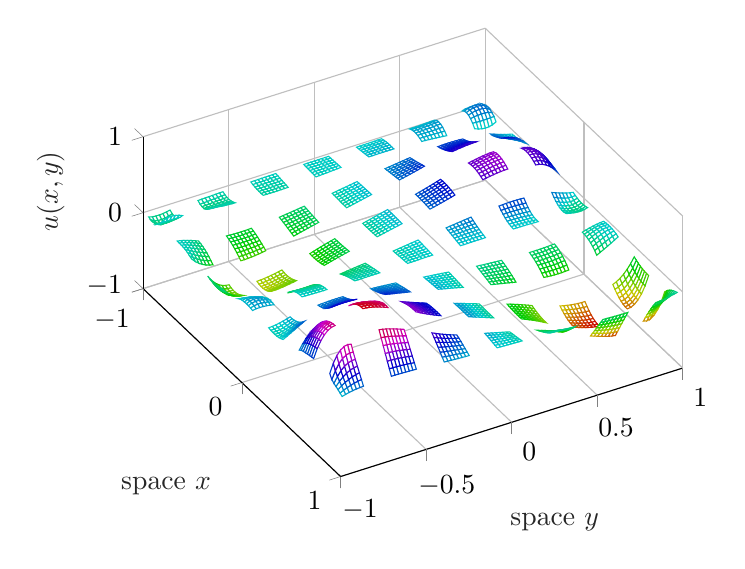
\begin{tikzpicture}

\begin{axis}[%
unbounded coords=jump,
xmin=-1,
xmax=1,
tick align=outside,
xlabel style={font=\color{white!15!black}},
xlabel={space $x$},
ymin=-1,
ymax=1,
ylabel style={font=\color{white!15!black}},
ylabel={space $y$},
zmin=-1,
zmax=1,
zlabel style={font=\color{white!15!black}},
zlabel={$u(x,y)$},
view={60}{55},
axis background/.style={fill=white},
axis x line*=bottom,
axis y line*=left,
axis z line*=left,
xmajorgrids,
ymajorgrids,
zmajorgrids,
\extraAxisOptions
]

\addplot3[%
surf,
shader=flat corner, fill=white, z buffer=sort, colormap={mymap}{[1pt] rgb(0pt)=(0.8,0,0); rgb(10pt)=(0.8,0.75,0); rgb(11pt)=(0.775,0.8,0); rgb(21pt)=(0.025,0.8,0); rgb(22pt)=(0,0.8,0.05); rgb(32pt)=(0,0.8,0.8); rgb(42pt)=(0,0.05,0.8); rgb(43pt)=(0.025,0,0.8); rgb(53pt)=(0.775,0,0.8); rgb(54pt)=(0.8,0,0.75); rgb(63pt)=(0.8,0,0.075)}, mesh/rows=63]
table[row sep=crcr, point meta=\thisrow{c}] {%
%
x	y	z	c\\
-1	-1	nan	nan\\
-1	-0.979166666666667	nan	nan\\
-1	-0.958333333333333	nan	nan\\
-1	-0.9375	nan	nan\\
-1	-0.916666666666667	nan	nan\\
-1	-0.895833333333333	nan	nan\\
-1	-0.875	nan	nan\\
-1	-0.854166666666667	nan	nan\\
-1	nan	nan	nan\\
-1	-0.690972222222222	nan	nan\\
-1	-0.670138888888889	nan	nan\\
-1	-0.649305555555556	nan	nan\\
-1	-0.628472222222222	nan	nan\\
-1	-0.607638888888889	nan	nan\\
-1	-0.586805555555556	nan	nan\\
-1	-0.565972222222222	nan	nan\\
-1	-0.545138888888889	nan	nan\\
-1	nan	nan	nan\\
-1	-0.381944444444444	nan	nan\\
-1	-0.361111111111111	nan	nan\\
-1	-0.340277777777778	nan	nan\\
-1	-0.319444444444444	nan	nan\\
-1	-0.298611111111111	nan	nan\\
-1	-0.277777777777778	nan	nan\\
-1	-0.256944444444444	nan	nan\\
-1	-0.236111111111111	nan	nan\\
-1	nan	nan	nan\\
-1	-0.0729166666666667	nan	nan\\
-1	-0.0520833333333333	nan	nan\\
-1	-0.03125	nan	nan\\
-1	-0.0104166666666667	nan	nan\\
-1	0.0104166666666667	nan	nan\\
-1	0.03125	nan	nan\\
-1	0.0520833333333333	nan	nan\\
-1	0.0729166666666667	nan	nan\\
-1	nan	nan	nan\\
-1	0.236111111111111	nan	nan\\
-1	0.256944444444444	nan	nan\\
-1	0.277777777777778	nan	nan\\
-1	0.298611111111111	nan	nan\\
-1	0.319444444444444	nan	nan\\
-1	0.340277777777778	nan	nan\\
-1	0.361111111111111	nan	nan\\
-1	0.381944444444444	nan	nan\\
-1	nan	nan	nan\\
-1	0.545138888888889	nan	nan\\
-1	0.565972222222222	nan	nan\\
-1	0.586805555555556	nan	nan\\
-1	0.607638888888889	nan	nan\\
-1	0.628472222222222	nan	nan\\
-1	0.649305555555556	nan	nan\\
-1	0.670138888888889	nan	nan\\
-1	0.690972222222222	nan	nan\\
-1	nan	nan	nan\\
-1	0.854166666666667	nan	nan\\
-1	0.875	nan	nan\\
-1	0.895833333333333	nan	nan\\
-1	0.916666666666667	nan	nan\\
-1	0.9375	nan	nan\\
-1	0.958333333333333	nan	nan\\
-1	0.979166666666667	nan	nan\\
-1	1	nan	nan\\
-1	nan	nan	nan\\
-0.979166666666667	-1	nan	nan\\
-0.979166666666667	-0.979166666666667	-0.0445599415901429	-0.0445599415901429\\
-0.979166666666667	-0.958333333333333	-0.0587531239098606	-0.0587531239098606\\
-0.979166666666667	-0.9375	-0.062918257429132	-0.062918257429132\\
-0.979166666666667	-0.916666666666667	-0.0636230912425222	-0.0636230912425222\\
-0.979166666666667	-0.895833333333333	-0.0604865926483698	-0.0604865926483698\\
-0.979166666666667	-0.875	-0.052909128157571	-0.052909128157571\\
-0.979166666666667	-0.854166666666667	-0.044037218571993	-0.044037218571993\\
-0.979166666666667	nan	nan	nan\\
-0.979166666666667	-0.690972222222222	-0.0351225972482386	-0.0351225972482386\\
-0.979166666666667	-0.670138888888889	-0.0327377393661455	-0.0327377393661455\\
-0.979166666666667	-0.649305555555556	-0.030989722937633	-0.030989722937633\\
-0.979166666666667	-0.628472222222222	-0.0295761299696657	-0.0295761299696657\\
-0.979166666666667	-0.607638888888889	-0.0280018522429253	-0.0280018522429253\\
-0.979166666666667	-0.586805555555556	-0.0260589208115868	-0.0260589208115868\\
-0.979166666666667	-0.565972222222222	-0.0241532283489252	-0.0241532283489252\\
-0.979166666666667	-0.545138888888889	-0.0227899784822621	-0.0227899784822621\\
-0.979166666666667	nan	nan	nan\\
-0.979166666666667	-0.381944444444444	-0.0115403812148842	-0.0115403812148842\\
-0.979166666666667	-0.361111111111111	-0.0102133730595972	-0.0102133730595972\\
-0.979166666666667	-0.340277777777778	-0.00939313636286308	-0.00939313636286308\\
-0.979166666666667	-0.319444444444444	-0.00878261613804039	-0.00878261613804039\\
-0.979166666666667	-0.298611111111111	-0.00806750828944576	-0.00806750828944576\\
-0.979166666666667	-0.277777777777778	-0.0070376490805122	-0.0070376490805122\\
-0.979166666666667	-0.256944444444444	-0.00577872310894662	-0.00577872310894662\\
-0.979166666666667	-0.236111111111111	-0.00467118900208902	-0.00467118900208902\\
-0.979166666666667	nan	nan	nan\\
-0.979166666666667	-0.0729166666666667	-0.00130872481607756	-0.00130872481607756\\
-0.979166666666667	-0.0520833333333333	-0.000850547042464292	-0.000850547042464292\\
-0.979166666666667	-0.03125	-0.000534598169010601	-0.000534598169010601\\
-0.979166666666667	-0.0104166666666667	-0.000287491446954447	-0.000287491446954447\\
-0.979166666666667	0.0104166666666667	3.47379707166306e-05	3.47379707166306e-05\\
-0.979166666666667	0.03125	0.000518889363691127	0.000518889363691127\\
-0.979166666666667	0.0520833333333333	0.00108203604230183	0.00108203604230183\\
-0.979166666666667	0.0729166666666667	0.00155270807313588	0.00155270807313588\\
-0.979166666666667	nan	nan	nan\\
-0.979166666666667	0.236111111111111	0.00478385600692974	0.00478385600692974\\
-0.979166666666667	0.256944444444444	0.00617570325292273	0.00617570325292273\\
-0.979166666666667	0.277777777777778	0.0069735969029102	0.0069735969029102\\
-0.979166666666667	0.298611111111111	0.00756618460304638	0.00756618460304638\\
-0.979166666666667	0.319444444444444	0.00829757660504597	0.00829757660504597\\
-0.979166666666667	0.340277777777778	0.00939357568385042	0.00939357568385042\\
-0.979166666666667	0.361111111111111	0.0107637235598528	0.0107637235598528\\
-0.979166666666667	0.381944444444444	0.0120334938518341	0.0120334938518341\\
-0.979166666666667	nan	nan	nan\\
-0.979166666666667	0.545138888888889	0.0241553050551976	0.0241553050551976\\
-0.979166666666667	0.565972222222222	0.0249318206507998	0.0249318206507998\\
-0.979166666666667	0.586805555555556	0.025996754053741	0.025996754053741\\
-0.979166666666667	0.607638888888889	0.0271395575134753	0.0271395575134753\\
-0.979166666666667	0.628472222222222	0.0286925706547467	0.0286925706547467\\
-0.979166666666667	0.649305555555556	0.0310309519647767	0.0310309519647767\\
-0.979166666666667	0.670138888888889	0.0338599883714049	0.0338599883714049\\
-0.979166666666667	0.690972222222222	0.0363264127143366	0.0363264127143366\\
-0.979166666666667	nan	nan	nan\\
-0.979166666666667	0.854166666666667	0.0411690277008248	0.0411690277008248\\
-0.979166666666667	0.875	0.0554133833815373	0.0554133833815373\\
-0.979166666666667	0.895833333333333	0.0613330807826334	0.0613330807826334\\
-0.979166666666667	0.916666666666667	0.0638211674503612	0.0638211674503612\\
-0.979166666666667	0.9375	0.06354764420453	0.06354764420453\\
-0.979166666666667	0.958333333333333	0.0558380273187589	0.0558380273187589\\
-0.979166666666667	0.979166666666667	0.0344848993958728	0.0344848993958728\\
-0.979166666666667	1	nan	nan\\
-0.979166666666667	nan	nan	nan\\
-0.958333333333333	-1	nan	nan\\
-0.958333333333333	-0.979166666666667	-0.0582056531600509	-0.0582056531600509\\
-0.958333333333333	-0.958333333333333	-0.0854026682063883	-0.0854026682063883\\
-0.958333333333333	-0.9375	-0.0957753023778436	-0.0957753023778436\\
-0.958333333333333	-0.916666666666667	-0.0976039457126222	-0.0976039457126222\\
-0.958333333333333	-0.895833333333333	-0.0928880795713706	-0.0928880795713706\\
-0.958333333333333	-0.875	-0.0820224885209548	-0.0820224885209548\\
-0.958333333333333	-0.854166666666667	-0.0656558446117515	-0.0656558446117515\\
-0.958333333333333	nan	nan	nan\\
-0.958333333333333	-0.690972222222222	-0.0569048549758185	-0.0569048549758185\\
-0.958333333333333	-0.670138888888889	-0.0535925609143025	-0.0535925609143025\\
-0.958333333333333	-0.649305555555556	-0.0506871034773638	-0.0506871034773638\\
-0.958333333333333	-0.628472222222222	-0.0481086068754751	-0.0481086068754751\\
-0.958333333333333	-0.607638888888889	-0.0455182596082115	-0.0455182596082115\\
-0.958333333333333	-0.586805555555556	-0.0428628688647365	-0.0428628688647365\\
-0.958333333333333	-0.565972222222222	-0.0405315958030697	-0.0405315958030697\\
-0.958333333333333	-0.545138888888889	-0.0390331357119047	-0.0390331357119047\\
-0.958333333333333	nan	nan	nan\\
-0.958333333333333	-0.381944444444444	-0.0207726095658704	-0.0207726095658704\\
-0.958333333333333	-0.361111111111111	-0.0187960548144446	-0.0187960548144446\\
-0.958333333333333	-0.340277777777778	-0.0172567582873383	-0.0172567582873383\\
-0.958333333333333	-0.319444444444444	-0.0159476825862986	-0.0159476825862986\\
-0.958333333333333	-0.298611111111111	-0.0145716367452924	-0.0145716367452924\\
-0.958333333333333	-0.277777777777778	-0.0129652895843328	-0.0129652895843328\\
-0.958333333333333	-0.256944444444444	-0.011152188935864	-0.011152188935864\\
-0.958333333333333	-0.236111111111111	-0.00922402268210385	-0.00922402268210385\\
-0.958333333333333	nan	nan	nan\\
-0.958333333333333	-0.0729166666666667	-0.00276526825451223	-0.00276526825451223\\
-0.958333333333333	-0.0520833333333333	-0.00194798477524921	-0.00194798477524921\\
-0.958333333333333	-0.03125	-0.00118475239473505	-0.00118475239473505\\
-0.958333333333333	-0.0104166666666667	-0.00046241491128415	-0.00046241491128415\\
-0.958333333333333	0.0104166666666667	0.000316388431216587	0.000316388431216587\\
-0.958333333333333	0.03125	0.00117311524904568	0.00117311524904568\\
-0.958333333333333	0.0520833333333333	0.00204142708868761	0.00204142708868761\\
-0.958333333333333	0.0729166666666667	0.00284599740287464	0.00284599740287464\\
-0.958333333333333	nan	nan	nan\\
-0.958333333333333	0.236111111111111	0.00928108267782025	0.00928108267782025\\
-0.958333333333333	0.256944444444444	0.0113238526408241	0.0113238526408241\\
-0.958333333333333	0.277777777777778	0.0128810174015283	0.0128810174015283\\
-0.958333333333333	0.298611111111111	0.0142025565688102	0.0142025565688102\\
-0.958333333333333	0.319444444444444	0.0156132142657473	0.0156132142657473\\
-0.958333333333333	0.340277777777778	0.0172792175818445	0.0172792175818445\\
-0.958333333333333	0.361111111111111	0.0191496903164377	0.0191496903164377\\
-0.958333333333333	0.381944444444444	0.0210812313535185	0.0210812313535185\\
-0.958333333333333	nan	nan	nan\\
-0.958333333333333	0.545138888888889	0.0399415252741587	0.0399415252741587\\
-0.958333333333333	0.565972222222222	0.0411370345975099	0.0411370345975099\\
-0.958333333333333	0.586805555555556	0.0428497410896174	0.0428497410896174\\
-0.958333333333333	0.607638888888889	0.0449090037731407	0.0449090037731407\\
-0.958333333333333	0.628472222222222	0.0475118411478544	0.0475118411478544\\
-0.958333333333333	0.649305555555556	0.050790205157561	0.050790205157561\\
-0.958333333333333	0.670138888888889	0.0544107972823837	0.0544107972823837\\
-0.958333333333333	0.690972222222222	0.0577604234383709	0.0577604234383709\\
-0.958333333333333	nan	nan	nan\\
-0.958333333333333	0.854166666666667	0.0641784114554647	0.0641784114554647\\
-0.958333333333333	0.875	0.0832783957238558	0.0832783957238558\\
-0.958333333333333	0.895833333333333	0.0936935596951311	0.0936935596951311\\
-0.958333333333333	0.916666666666667	0.097884980767432	0.097884980767432\\
-0.958333333333333	0.9375	0.0956359551471065	0.0956359551471065\\
-0.958333333333333	0.958333333333333	0.0824899606581817	0.0824899606581817\\
-0.958333333333333	0.979166666666667	0.052482493107942	0.052482493107942\\
-0.958333333333333	1	nan	nan\\
-0.958333333333333	nan	nan	nan\\
-0.9375	-1	nan	nan\\
-0.9375	-0.979166666666667	-0.0604400974350717	-0.0604400974350717\\
-0.9375	-0.958333333333333	-0.0913400858763807	-0.0913400858763807\\
-0.9375	-0.9375	-0.104173056151223	-0.104173056151223\\
-0.9375	-0.916666666666667	-0.106662961466532	-0.106662961466532\\
-0.9375	-0.895833333333333	-0.101709073517642	-0.101709073517642\\
-0.9375	-0.875	-0.0901140769665484	-0.0901140769665484\\
-0.9375	-0.854166666666667	-0.0718000443957584	-0.0718000443957584\\
-0.9375	nan	nan	nan\\
-0.9375	-0.690972222222222	-0.0653992208253332	-0.0653992208253332\\
-0.9375	-0.670138888888889	-0.0620270340264217	-0.0620270340264217\\
-0.9375	-0.649305555555556	-0.0590320602102594	-0.0590320602102594\\
-0.9375	-0.628472222222222	-0.0563673675176083	-0.0563673675176083\\
-0.9375	-0.607638888888889	-0.0537063674625187	-0.0537063674625187\\
-0.9375	-0.586805555555556	-0.0510167429109778	-0.0510167429109778\\
-0.9375	-0.565972222222222	-0.0486986741392566	-0.0486986741392566\\
-0.9375	-0.545138888888889	-0.0473189026529827	-0.0473189026529827\\
-0.9375	nan	nan	nan\\
-0.9375	-0.381944444444444	-0.027415702553517	-0.027415702553517\\
-0.9375	-0.361111111111111	-0.0252500723616506	-0.0252500723616506\\
-0.9375	-0.340277777777778	-0.0234121792441195	-0.0234121792441195\\
-0.9375	-0.319444444444444	-0.021717010728345	-0.021717010728345\\
-0.9375	-0.298611111111111	-0.0199872707409415	-0.0199872707409415\\
-0.9375	-0.277777777777778	-0.0181225767770021	-0.0181225767770021\\
-0.9375	-0.256944444444444	-0.0160725385697254	-0.0160725385697254\\
-0.9375	-0.236111111111111	-0.0137605386308919	-0.0137605386308919\\
-0.9375	nan	nan	nan\\
-0.9375	-0.0729166666666667	-0.00429979687116618	-0.00429979687116618\\
-0.9375	-0.0520833333333333	-0.00318612603137202	-0.00318612603137202\\
-0.9375	-0.03125	-0.00192146508721572	-0.00192146508721572\\
-0.9375	-0.0104166666666667	-0.000563871969548879	-0.000563871969548879\\
-0.9375	0.0104166666666667	0.000726048603785432	0.000726048603785432\\
-0.9375	0.03125	0.00189034368555617	0.00189034368555617\\
-0.9375	0.0520833333333333	0.00298669248807272	0.00298669248807272\\
-0.9375	0.0729166666666667	0.00407770083391098	0.00407770083391098\\
-0.9375	nan	nan	nan\\
-0.9375	0.236111111111111	0.0136497093398052	0.0136497093398052\\
-0.9375	0.256944444444444	0.0159949451137944	0.0159949451137944\\
-0.9375	0.277777777777778	0.0179975037530082	0.0179975037530082\\
-0.9375	0.298611111111111	0.0198026205250388	0.0198026205250388\\
-0.9375	0.319444444444444	0.021568250471852	0.021568250471852\\
-0.9375	0.340277777777778	0.0234399922768961	0.0234399922768961\\
-0.9375	0.361111111111111	0.0254580198533061	0.0254580198533061\\
-0.9375	0.381944444444444	0.0275699604726387	0.0275699604726387\\
-0.9375	nan	nan	nan\\
-0.9375	0.545138888888889	0.0480867686613332	0.0480867686613332\\
-0.9375	0.565972222222222	0.0492855256965939	0.0492855256965939\\
-0.9375	0.586805555555556	0.0510021649468524	0.0510021649468524\\
-0.9375	0.607638888888889	0.0531011425825351	0.0531011425825351\\
-0.9375	0.628472222222222	0.0557849143005136	0.0557849143005136\\
-0.9375	0.649305555555556	0.0591427957960838	0.0591427957960838\\
-0.9375	0.670138888888889	0.0628268456517453	0.0628268456517453\\
-0.9375	0.690972222222222	0.0662451191205794	0.0662451191205794\\
-0.9375	nan	nan	nan\\
-0.9375	0.854166666666667	0.0710529550748937	0.0710529550748937\\
-0.9375	0.875	0.0910600833310619	0.0910600833310619\\
-0.9375	0.895833333333333	0.102449742679154	0.102449742679154\\
-0.9375	0.916666666666667	0.106867923879796	0.106867923879796\\
-0.9375	0.9375	0.103720171113615	0.103720171113615\\
-0.9375	0.958333333333333	0.0889289832156704	0.0889289832156704\\
-0.9375	0.979166666666667	0.0566767619584848	0.0566767619584848\\
-0.9375	1	nan	nan\\
-0.9375	nan	nan	nan\\
-0.916666666666667	-1	nan	nan\\
-0.916666666666667	-0.979166666666667	-0.055679231915459	-0.055679231915459\\
-0.916666666666667	-0.958333333333333	-0.0814346585113227	-0.0814346585113227\\
-0.916666666666667	-0.9375	-0.0912930943894773	-0.0912930943894773\\
-0.916666666666667	-0.916666666666667	-0.0934621582052787	-0.0934621582052787\\
-0.916666666666667	-0.895833333333333	-0.0894797292710013	-0.0894797292710013\\
-0.916666666666667	-0.875	-0.0793637030233114	-0.0793637030233114\\
-0.916666666666667	-0.854166666666667	-0.0647546584873538	-0.0647546584873538\\
-0.916666666666667	nan	nan	nan\\
-0.916666666666667	-0.690972222222222	-0.0614158243660456	-0.0614158243660456\\
-0.916666666666667	-0.670138888888889	-0.058712318171349	-0.058712318171349\\
-0.916666666666667	-0.649305555555556	-0.0566478808119774	-0.0566478808119774\\
-0.916666666666667	-0.628472222222222	-0.0549883093291484	-0.0549883093291484\\
-0.916666666666667	-0.607638888888889	-0.0531544431045781	-0.0531544431045781\\
-0.916666666666667	-0.586805555555556	-0.0509893896915623	-0.0509893896915623\\
-0.916666666666667	-0.565972222222222	-0.0490114486244904	-0.0490114486244904\\
-0.916666666666667	-0.545138888888889	-0.0478594521144028	-0.0478594521144028\\
-0.916666666666667	nan	nan	nan\\
-0.916666666666667	-0.381944444444444	-0.0315490330013433	-0.0315490330013433\\
-0.916666666666667	-0.361111111111111	-0.0295504459551184	-0.0295504459551184\\
-0.916666666666667	-0.340277777777778	-0.0278876631731465	-0.0278876631731465\\
-0.916666666666667	-0.319444444444444	-0.0263074150650525	-0.0263074150650525\\
-0.916666666666667	-0.298611111111111	-0.0245961688596077	-0.0245961688596077\\
-0.916666666666667	-0.277777777777778	-0.0226811307669374	-0.0226811307669374\\
-0.916666666666667	-0.256944444444444	-0.0205569747657809	-0.0205569747657809\\
-0.916666666666667	-0.236111111111111	-0.018193330007362	-0.018193330007362\\
-0.916666666666667	nan	nan	nan\\
-0.916666666666667	-0.0729166666666667	-0.0058444247336082	-0.0058444247336082\\
-0.916666666666667	-0.0520833333333333	-0.00436382647481454	-0.00436382647481454\\
-0.916666666666667	-0.03125	-0.00261585199237209	-0.00261585199237209\\
-0.916666666666667	-0.0104166666666667	-0.000732873914000793	-0.000732873914000793\\
-0.916666666666667	0.0104166666666667	0.00104946196917299	0.00104946196917299\\
-0.916666666666667	0.03125	0.00259728751264889	0.00259728751264889\\
-0.916666666666667	0.0520833333333333	0.00400745016888686	0.00400745016888686\\
-0.916666666666667	0.0729166666666667	0.0054793797722505	0.0054793797722505\\
-0.916666666666667	nan	nan	nan\\
-0.916666666666667	0.236111111111111	0.0179993616282841	0.0179993616282841\\
-0.916666666666667	0.256944444444444	0.020476580442393	0.020476580442393\\
-0.916666666666667	0.277777777777778	0.022551956545043	0.022551956545043\\
-0.916666666666667	0.298611111111111	0.0243686629658639	0.0243686629658639\\
-0.916666666666667	0.319444444444444	0.0261054666105969	0.0261054666105969\\
-0.916666666666667	0.340277777777778	0.027927841050438	0.027927841050438\\
-0.916666666666667	0.361111111111111	0.0298674449095493	0.0298674449095493\\
-0.916666666666667	0.381944444444444	0.0317734647899909	0.0317734647899909\\
-0.916666666666667	nan	nan	nan\\
-0.916666666666667	0.545138888888889	0.0490362233622039	0.0490362233622039\\
-0.916666666666667	0.565972222222222	0.0498292521539052	0.0498292521539052\\
-0.916666666666667	0.586805555555556	0.0509273300753472	0.0509273300753472\\
-0.916666666666667	0.607638888888889	0.0521935702848153	0.0521935702848153\\
-0.916666666666667	0.628472222222222	0.0540232319377975	0.0540232319377975\\
-0.916666666666667	0.649305555555556	0.05672463110813	0.05672463110813\\
-0.916666666666667	0.670138888888889	0.0598939542151984	0.0598939542151984\\
-0.916666666666667	0.690972222222222	0.0627106219450167	0.0627106219450167\\
-0.916666666666667	nan	nan	nan\\
-0.916666666666667	0.854166666666667	0.0633917769233674	0.0633917769233674\\
-0.916666666666667	0.875	0.0814336856316035	0.0814336856316035\\
-0.916666666666667	0.895833333333333	0.0904440608013186	0.0904440608013186\\
-0.916666666666667	0.916666666666667	0.0938869292383453	0.0938869292383453\\
-0.916666666666667	0.9375	0.0917543226896981	0.0917543226896981\\
-0.916666666666667	0.958333333333333	0.0789867724431987	0.0789867724431987\\
-0.916666666666667	0.979166666666667	0.0494751031972505	0.0494751031972505\\
-0.916666666666667	1	nan	nan\\
-0.916666666666667	nan	nan	nan\\
-0.895833333333333	-1	nan	nan\\
-0.895833333333333	-0.979166666666667	-0.0382871747470283	-0.0382871747470283\\
-0.895833333333333	-0.958333333333333	-0.0534453769218254	-0.0534453769218254\\
-0.895833333333333	-0.9375	-0.0582882106937488	-0.0582882106937488\\
-0.895833333333333	-0.916666666666667	-0.0589999495506584	-0.0589999495506584\\
-0.895833333333333	-0.895833333333333	-0.0569064616340711	-0.0569064616340711\\
-0.895833333333333	-0.875	-0.0516034990404691	-0.0516034990404691\\
-0.895833333333333	-0.854166666666667	-0.0438290474102176	-0.0438290474102176\\
-0.895833333333333	nan	nan	nan\\
-0.895833333333333	-0.690972222222222	-0.0463589356006789	-0.0463589356006789\\
-0.895833333333333	-0.670138888888889	-0.0453579667027081	-0.0453579667027081\\
-0.895833333333333	-0.649305555555556	-0.0448091910108112	-0.0448091910108112\\
-0.895833333333333	-0.628472222222222	-0.0444714652745971	-0.0444714652745971\\
-0.895833333333333	-0.607638888888889	-0.0440021934971596	-0.0440021934971596\\
-0.895833333333333	-0.586805555555556	-0.0432234119413738	-0.0432234119413738\\
-0.895833333333333	-0.565972222222222	-0.0424445487082794	-0.0424445487082794\\
-0.895833333333333	-0.545138888888889	-0.0422036641881153	-0.0422036641881153\\
-0.895833333333333	nan	nan	nan\\
-0.895833333333333	-0.381944444444444	-0.0335579577589252	-0.0335579577589252\\
-0.895833333333333	-0.361111111111111	-0.032224344053716	-0.032224344053716\\
-0.895833333333333	-0.340277777777778	-0.0310291116252512	-0.0310291116252512\\
-0.895833333333333	-0.319444444444444	-0.0297864535889407	-0.0297864535889407\\
-0.895833333333333	-0.298611111111111	-0.0283536760046269	-0.0283536760046269\\
-0.895833333333333	-0.277777777777778	-0.0266596449396096	-0.0266596449396096\\
-0.895833333333333	-0.256944444444444	-0.0247100007252573	-0.0247100007252573\\
-0.895833333333333	-0.236111111111111	-0.0225125368039617	-0.0225125368039617\\
-0.895833333333333	nan	nan	nan\\
-0.895833333333333	-0.0729166666666667	-0.00734606894445484	-0.00734606894445484\\
-0.895833333333333	-0.0520833333333333	-0.00536903545974525	-0.00536903545974525\\
-0.895833333333333	-0.03125	-0.00322818092559749	-0.00322818092559749\\
-0.895833333333333	-0.0104166666666667	-0.00101889191633735	-0.00101889191633735\\
-0.895833333333333	0.0104166666666667	0.00116091742196074	0.00116091742196074\\
-0.895833333333333	0.03125	0.00322103743200849	0.00322103743200849\\
-0.895833333333333	0.0520833333333333	0.00517981260472279	0.00517981260472279\\
-0.895833333333333	0.0729166666666667	0.00715519718501433	0.00715519718501433\\
-0.895833333333333	nan	nan	nan\\
-0.895833333333333	0.236111111111111	0.0224232465048296	0.0224232465048296\\
-0.895833333333333	0.256944444444444	0.024710289067667	0.024710289067667\\
-0.895833333333333	0.277777777777778	0.0265630242394948	0.0265630242394948\\
-0.895833333333333	0.298611111111111	0.0281437311577644	0.0281437311577644\\
-0.895833333333333	0.319444444444444	0.0295945748754842	0.0295945748754842\\
-0.895833333333333	0.340277777777778	0.0310365320252159	0.0310365320252159\\
-0.895833333333333	0.361111111111111	0.0324725937000036	0.0324725937000036\\
-0.895833333333333	0.381944444444444	0.0337383424616729	0.0337383424616729\\
-0.895833333333333	nan	nan	nan\\
-0.895833333333333	0.545138888888889	0.0430077214603163	0.0430077214603163\\
-0.895833333333333	0.565972222222222	0.0429813982784521	0.0429813982784521\\
-0.895833333333333	0.586805555555556	0.0431309585639506	0.0431309585639506\\
-0.895833333333333	0.607638888888889	0.0433320692937216	0.0433320692937216\\
-0.895833333333333	0.628472222222222	0.0437908089599185	0.0437908089599185\\
-0.895833333333333	0.649305555555556	0.0447807600842341	0.0447807600842341\\
-0.895833333333333	0.670138888888889	0.0461246782133643	0.0461246782133643\\
-0.895833333333333	0.690972222222222	0.0472101301447878	0.0472101301447878\\
-0.895833333333333	nan	nan	nan\\
-0.895833333333333	0.854166666666667	0.0427466425481225	0.0427466425481225\\
-0.895833333333333	0.875	0.0530663590945928	0.0530663590945928\\
-0.895833333333333	0.895833333333333	0.0574807814085975	0.0574807814085975\\
-0.895833333333333	0.916666666666667	0.059341097302564	0.059341097302564\\
-0.895833333333333	0.9375	0.0587349900833343	0.0587349900833343\\
-0.895833333333333	0.958333333333333	0.0520145406936319	0.0520145406936319\\
-0.895833333333333	0.979166666666667	0.0337698639727987	0.0337698639727987\\
-0.895833333333333	1	nan	nan\\
-0.895833333333333	nan	nan	nan\\
-0.875	-1	nan	nan\\
-0.875	-0.979166666666667	-0.00499834821595816	-0.00499834821595816\\
-0.875	-0.958333333333333	-0.0057855924598559	-0.0057855924598559\\
-0.875	-0.9375	-0.00439122950532836	-0.00439122950532836\\
-0.875	-0.916666666666667	-0.00293427948573439	-0.00293427948573439\\
-0.875	-0.895833333333333	-0.00375877325234174	-0.00375877325234174\\
-0.875	-0.875	-0.00707062733314802	-0.00707062733314802\\
-0.875	-0.854166666666667	-0.00874073545482729	-0.00874073545482729\\
-0.875	nan	nan	nan\\
-0.875	-0.690972222222222	-0.0213655117898855	-0.0213655117898855\\
-0.875	-0.670138888888889	-0.0230657861449416	-0.0230657861449416\\
-0.875	-0.649305555555556	-0.0245458179853679	-0.0245458179853679\\
-0.875	-0.628472222222222	-0.0258804267066173	-0.0258804267066173\\
-0.875	-0.607638888888889	-0.0272451941961974	-0.0272451941961974\\
-0.875	-0.586805555555556	-0.0286625369262729	-0.0286625369262729\\
-0.875	-0.565972222222222	-0.0299912520081525	-0.0299912520081525\\
-0.875	-0.545138888888889	-0.0313231604560568	-0.0313231604560568\\
-0.875	nan	nan	nan\\
-0.875	-0.381944444444444	-0.0338784001517414	-0.0338784001517414\\
-0.875	-0.361111111111111	-0.0336368016843357	-0.0336368016843357\\
-0.875	-0.340277777777778	-0.0330981172673102	-0.0330981172673102\\
-0.875	-0.319444444444444	-0.03233209089184	-0.03233209089184\\
-0.875	-0.298611111111111	-0.0313550678790968	-0.0313550678790968\\
-0.875	-0.277777777777778	-0.0301353580163462	-0.0301353580163462\\
-0.875	-0.256944444444444	-0.0286488990936392	-0.0286488990936392\\
-0.875	-0.236111111111111	-0.026805362633579	-0.026805362633579\\
-0.875	nan	nan	nan\\
-0.875	-0.0729166666666667	-0.0088588385513951	-0.0088588385513951\\
-0.875	-0.0520833333333333	-0.00630802590975546	-0.00630802590975546\\
-0.875	-0.03125	-0.00382555012047417	-0.00382555012047417\\
-0.875	-0.0104166666666667	-0.00135814555916366	-0.00135814555916366\\
-0.875	0.0104166666666667	0.00116377844006256	0.00116377844006256\\
-0.875	0.03125	0.00379800116309481	0.00379800116309481\\
-0.875	0.0520833333333333	0.0064764834238844	0.0064764834238844\\
-0.875	0.0729166666666667	0.00900598004751173	0.00900598004751173\\
-0.875	nan	nan	nan\\
-0.875	0.236111111111111	0.0269774807678944	0.0269774807678944\\
-0.875	0.256944444444444	0.028664256848552	0.028664256848552\\
-0.875	0.277777777777778	0.0300921708741696	0.0300921708741696\\
-0.875	0.298611111111111	0.0312947529746224	0.0312947529746224\\
-0.875	0.319444444444444	0.0322894369743959	0.0322894369743959\\
-0.875	0.340277777777778	0.0330650492416326	0.0330650492416326\\
-0.875	0.361111111111111	0.0335723082223994	0.0335723082223994\\
-0.875	0.381944444444444	0.0338298390296258	0.0338298390296258\\
-0.875	nan	nan	nan\\
-0.875	0.545138888888889	0.0308027268713476	0.0308027268713476\\
-0.875	0.565972222222222	0.02973942206348	0.02973942206348\\
-0.875	0.586805555555556	0.0286305477285964	0.0286305477285964\\
-0.875	0.607638888888889	0.0274945289029251	0.0274945289029251\\
-0.875	0.628472222222222	0.0261549251676929	0.0261549251676929\\
-0.875	0.649305555555556	0.024454067097961	0.024454067097961\\
-0.875	0.670138888888889	0.0225305450647145	0.0225305450647145\\
-0.875	0.690972222222222	0.0207735580504226	0.0207735580504226\\
-0.875	nan	nan	nan\\
-0.875	0.854166666666667	0.00960424744333529	0.00960424744333529\\
-0.875	0.875	0.00535968022176972	0.00535968022176972\\
-0.875	0.895833333333333	0.00350612935715456	0.00350612935715456\\
-0.875	0.916666666666667	0.00307278228798872	0.00307278228798872\\
-0.875	0.9375	0.00366169710754634	0.00366169710754634\\
-0.875	0.958333333333333	0.00589410021633079	0.00589410021633079\\
-0.875	0.979166666666667	0.0085884953360545	0.0085884953360545\\
-0.875	1	nan	nan\\
-0.875	nan	nan	nan\\
-0.854166666666667	-1	nan	nan\\
-0.854166666666667	-0.979166666666667	0.0355085219433251	0.0355085219433251\\
-0.854166666666667	-0.958333333333333	0.0601048544627872	0.0601048544627872\\
-0.854166666666667	-0.9375	0.0732627199251464	0.0732627199251464\\
-0.854166666666667	-0.916666666666667	0.0758370504630108	0.0758370504630108\\
-0.854166666666667	-0.895833333333333	0.0698547799901412	0.0698547799901412\\
-0.854166666666667	-0.875	0.0569395596992928	0.0569395596992928\\
-0.854166666666667	-0.854166666666667	0.0375791730988449	0.0375791730988449\\
-0.854166666666667	nan	nan	nan\\
-0.854166666666667	-0.690972222222222	0.0134094623969869	0.0134094623969869\\
-0.854166666666667	-0.670138888888889	0.00862659374547078	0.00862659374547078\\
-0.854166666666667	-0.649305555555556	0.00370746563598586	0.00370746563598586\\
-0.854166666666667	-0.628472222222222	-0.00110867778463871	-0.00110867778463871\\
-0.854166666666667	-0.607638888888889	-0.00547866619212576	-0.00547866619212576\\
-0.854166666666667	-0.586805555555556	-0.00919252639446501	-0.00919252639446501\\
-0.854166666666667	-0.565972222222222	-0.012195998719829	-0.012195998719829\\
-0.854166666666667	-0.545138888888889	-0.0144223417367608	-0.0144223417367608\\
-0.854166666666667	nan	nan	nan\\
-0.854166666666667	-0.381944444444444	-0.0327498626985441	-0.0327498626985441\\
-0.854166666666667	-0.361111111111111	-0.033574101727574	-0.033574101727574\\
-0.854166666666667	-0.340277777777778	-0.034117111371354	-0.034117111371354\\
-0.854166666666667	-0.319444444444444	-0.034367879194247	-0.034367879194247\\
-0.854166666666667	-0.298611111111111	-0.034143388082565	-0.034143388082565\\
-0.854166666666667	-0.277777777777778	-0.0334088915253396	-0.0334088915253396\\
-0.854166666666667	-0.256944444444444	-0.0323567578000792	-0.0323567578000792\\
-0.854166666666667	-0.236111111111111	-0.0312637340676501	-0.0312637340676501\\
-0.854166666666667	nan	nan	nan\\
-0.854166666666667	-0.0729166666666667	-0.0105241894380525	-0.0105241894380525\\
-0.854166666666667	-0.0520833333333333	-0.00741380322482836	-0.00741380322482836\\
-0.854166666666667	-0.03125	-0.00449446239002165	-0.00449446239002165\\
-0.854166666666667	-0.0104166666666667	-0.00166450394595935	-0.00166450394595935\\
-0.854166666666667	0.0104166666666667	0.00129277747204114	0.00129277747204114\\
-0.854166666666667	0.03125	0.00448316609816728	0.00448316609816728\\
-0.854166666666667	0.0520833333333333	0.00776437141589475	0.00776437141589475\\
-0.854166666666667	0.0729166666666667	0.0108799227005796	0.0108799227005796\\
-0.854166666666667	nan	nan	nan\\
-0.854166666666667	0.236111111111111	0.0315727247368313	0.0315727247368313\\
-0.854166666666667	0.256944444444444	0.0327019979905387	0.0327019979905387\\
-0.854166666666667	0.277777777777778	0.0334092497676202	0.0334092497676202\\
-0.854166666666667	0.298611111111111	0.0337739317027829	0.0337739317027829\\
-0.854166666666667	0.319444444444444	0.0339927196705704	0.0339927196705704\\
-0.854166666666667	0.340277777777778	0.0340991447560838	0.0340991447560838\\
-0.854166666666667	0.361111111111111	0.0338723266920296	0.0338723266920296\\
-0.854166666666667	0.381944444444444	0.0330280358343855	0.0330280358343855\\
-0.854166666666667	nan	nan	nan\\
-0.854166666666667	0.545138888888889	0.0146199171617091	0.0146199171617091\\
-0.854166666666667	0.565972222222222	0.0122990656923094	0.0122990656923094\\
-0.854166666666667	0.586805555555556	0.00910942750145905	0.00910942750145905\\
-0.854166666666667	0.607638888888889	0.00517621087368409	0.00517621087368409\\
-0.854166666666667	0.628472222222222	0.000794536417267341	0.000794536417267341\\
-0.854166666666667	0.649305555555556	-0.00386019532117612	-0.00386019532117612\\
-0.854166666666667	0.670138888888889	-0.00869176218816357	-0.00869176218816357\\
-0.854166666666667	0.690972222222222	-0.0134681867509183	-0.0134681867509183\\
-0.854166666666667	nan	nan	nan\\
-0.854166666666667	0.854166666666667	-0.038664306303588	-0.038664306303588\\
-0.854166666666667	0.875	-0.0572664000982909	-0.0572664000982909\\
-0.854166666666667	0.895833333333333	-0.0699790664372154	-0.0699790664372154\\
-0.854166666666667	0.916666666666667	-0.0754962367494589	-0.0754962367494589\\
-0.854166666666667	0.9375	-0.0728130963575776	-0.0728130963575776\\
-0.854166666666667	0.958333333333333	-0.0609738328168269	-0.0609738328168269\\
-0.854166666666667	0.979166666666667	-0.0379946827126653	-0.0379946827126653\\
-0.854166666666667	1	nan	nan\\
-0.854166666666667	nan	nan	nan\\
nan	-1	nan	nan\\
nan	-0.979166666666667	nan	nan\\
nan	-0.958333333333333	nan	nan\\
nan	-0.9375	nan	nan\\
nan	-0.916666666666667	nan	nan\\
nan	-0.895833333333333	nan	nan\\
nan	-0.875	nan	nan\\
nan	-0.854166666666667	nan	nan\\
nan	nan	nan	nan\\
nan	-0.690972222222222	nan	nan\\
nan	-0.670138888888889	nan	nan\\
nan	-0.649305555555556	nan	nan\\
nan	-0.628472222222222	nan	nan\\
nan	-0.607638888888889	nan	nan\\
nan	-0.586805555555556	nan	nan\\
nan	-0.565972222222222	nan	nan\\
nan	-0.545138888888889	nan	nan\\
nan	nan	nan	nan\\
nan	-0.381944444444444	nan	nan\\
nan	-0.361111111111111	nan	nan\\
nan	-0.340277777777778	nan	nan\\
nan	-0.319444444444444	nan	nan\\
nan	-0.298611111111111	nan	nan\\
nan	-0.277777777777778	nan	nan\\
nan	-0.256944444444444	nan	nan\\
nan	-0.236111111111111	nan	nan\\
nan	nan	nan	nan\\
nan	-0.0729166666666667	nan	nan\\
nan	-0.0520833333333333	nan	nan\\
nan	-0.03125	nan	nan\\
nan	-0.0104166666666667	nan	nan\\
nan	0.0104166666666667	nan	nan\\
nan	0.03125	nan	nan\\
nan	0.0520833333333333	nan	nan\\
nan	0.0729166666666667	nan	nan\\
nan	nan	nan	nan\\
nan	0.236111111111111	nan	nan\\
nan	0.256944444444444	nan	nan\\
nan	0.277777777777778	nan	nan\\
nan	0.298611111111111	nan	nan\\
nan	0.319444444444444	nan	nan\\
nan	0.340277777777778	nan	nan\\
nan	0.361111111111111	nan	nan\\
nan	0.381944444444444	nan	nan\\
nan	nan	nan	nan\\
nan	0.545138888888889	nan	nan\\
nan	0.565972222222222	nan	nan\\
nan	0.586805555555556	nan	nan\\
nan	0.607638888888889	nan	nan\\
nan	0.628472222222222	nan	nan\\
nan	0.649305555555556	nan	nan\\
nan	0.670138888888889	nan	nan\\
nan	0.690972222222222	nan	nan\\
nan	nan	nan	nan\\
nan	0.854166666666667	nan	nan\\
nan	0.875	nan	nan\\
nan	0.895833333333333	nan	nan\\
nan	0.916666666666667	nan	nan\\
nan	0.9375	nan	nan\\
nan	0.958333333333333	nan	nan\\
nan	0.979166666666667	nan	nan\\
nan	1	nan	nan\\
nan	nan	nan	nan\\
-0.690972222222222	-1	nan	nan\\
-0.690972222222222	-0.979166666666667	-0.00651051761007085	-0.00651051761007085\\
-0.690972222222222	-0.958333333333333	-0.0153971246846486	-0.0153971246846486\\
-0.690972222222222	-0.9375	-0.0274222531199396	-0.0274222531199396\\
-0.690972222222222	-0.916666666666667	-0.0423060774645728	-0.0423060774645728\\
-0.690972222222222	-0.895833333333333	-0.0589006384283516	-0.0589006384283516\\
-0.690972222222222	-0.875	-0.0761668976970201	-0.0761668976970201\\
-0.690972222222222	-0.854166666666667	-0.0946800544933034	-0.0946800544933034\\
-0.690972222222222	nan	nan	nan\\
-0.690972222222222	-0.690972222222222	-0.144973204780124	-0.144973204780124\\
-0.690972222222222	-0.670138888888889	-0.148050357303831	-0.148050357303831\\
-0.690972222222222	-0.649305555555556	-0.150383918608491	-0.150383918608491\\
-0.690972222222222	-0.628472222222222	-0.151904922903986	-0.151904922903986\\
-0.690972222222222	-0.607638888888889	-0.152416413146352	-0.152416413146352\\
-0.690972222222222	-0.586805555555556	-0.151769637358305	-0.151769637358305\\
-0.690972222222222	-0.565972222222222	-0.150081342730697	-0.150081342730697\\
-0.690972222222222	-0.545138888888889	-0.147622796815131	-0.147622796815131\\
-0.690972222222222	nan	nan	nan\\
-0.690972222222222	-0.381944444444444	-0.119596748610349	-0.119596748610349\\
-0.690972222222222	-0.361111111111111	-0.113828407463897	-0.113828407463897\\
-0.690972222222222	-0.340277777777778	-0.108151600778061	-0.108151600778061\\
-0.690972222222222	-0.319444444444444	-0.102425047634615	-0.102425047634615\\
-0.690972222222222	-0.298611111111111	-0.0965111029769568	-0.0965111029769568\\
-0.690972222222222	-0.277777777777778	-0.090344877061109	-0.090344877061109\\
-0.690972222222222	-0.256944444444444	-0.0840802595548285	-0.0840802595548285\\
-0.690972222222222	-0.236111111111111	-0.0780231216792416	-0.0780231216792416\\
-0.690972222222222	nan	nan	nan\\
-0.690972222222222	-0.0729166666666667	-0.0252144111446128	-0.0252144111446128\\
-0.690972222222222	-0.0520833333333333	-0.0179228549546366	-0.0179228549546366\\
-0.690972222222222	-0.03125	-0.0107738288867156	-0.0107738288867156\\
-0.690972222222222	-0.0104166666666667	-0.00367758468018687	-0.00367758468018687\\
-0.690972222222222	0.0104166666666667	0.00345802001408909	0.00345802001408909\\
-0.690972222222222	0.03125	0.0107170294507446	0.0107170294507446\\
-0.690972222222222	0.0520833333333333	0.0180681497792016	0.0180681497792016\\
-0.690972222222222	0.0729166666666667	0.0253620483893108	0.0253620483893108\\
-0.690972222222222	nan	nan	nan\\
-0.690972222222222	0.236111111111111	0.0782619814001965	0.0782619814001965\\
-0.690972222222222	0.256944444444444	0.0843345866304202	0.0843345866304202\\
-0.690972222222222	0.277777777777778	0.0902648856554321	0.0902648856554321\\
-0.690972222222222	0.298611111111111	0.0961192400605194	0.0961192400605194\\
-0.690972222222222	0.319444444444444	0.102019383965683	0.102019383965683\\
-0.690972222222222	0.340277777777778	0.10808361293139	0.10808361293139\\
-0.690972222222222	0.361111111111111	0.114183273732919	0.114183273732919\\
-0.690972222222222	0.381944444444444	0.119895904793223	0.119895904793223\\
-0.690972222222222	nan	nan	nan\\
-0.690972222222222	0.545138888888889	0.14802469632396	0.14802469632396\\
-0.690972222222222	0.565972222222222	0.150373635387579	0.150373635387579\\
-0.690972222222222	0.586805555555556	0.15163062822311	0.15163062822311\\
-0.690972222222222	0.607638888888889	0.151901328528593	0.151901328528593\\
-0.690972222222222	0.628472222222222	0.151381086479271	0.151381086479271\\
-0.690972222222222	0.649305555555556	0.150191549476356	0.150191549476356\\
-0.690972222222222	0.670138888888889	0.148195505623821	0.148195505623821\\
-0.690972222222222	0.690972222222222	0.145178004057387	0.145178004057387\\
-0.690972222222222	nan	nan	nan\\
-0.690972222222222	0.854166666666667	0.093538662434908	0.093538662434908\\
-0.690972222222222	0.875	0.076067654580252	0.076067654580252\\
-0.690972222222222	0.895833333333333	0.0588975095493334	0.0588975095493334\\
-0.690972222222222	0.916666666666667	0.0428928389148563	0.0428928389148563\\
-0.690972222222222	0.9375	0.0283258454095929	0.0283258454095929\\
-0.690972222222222	0.958333333333333	0.0148268291209426	0.0148268291209426\\
-0.690972222222222	0.979166666666667	0.00350454607862821	0.00350454607862821\\
-0.690972222222222	1	nan	nan\\
-0.690972222222222	nan	nan	nan\\
-0.670138888888889	-1	nan	nan\\
-0.670138888888889	-0.979166666666667	-0.00689037397723665	-0.00689037397723665\\
-0.670138888888889	-0.958333333333333	-0.0173743962277772	-0.0173743962277772\\
-0.670138888888889	-0.9375	-0.0305822266907362	-0.0305822266907362\\
-0.670138888888889	-0.916666666666667	-0.0465103655096919	-0.0465103655096919\\
-0.670138888888889	-0.895833333333333	-0.0643772691586672	-0.0643772691586672\\
-0.670138888888889	-0.875	-0.0832041427975651	-0.0832041427975651\\
-0.670138888888889	-0.854166666666667	-0.102616297929528	-0.102616297929528\\
-0.670138888888889	nan	nan	nan\\
-0.670138888888889	-0.690972222222222	-0.156322383793868	-0.156322383793868\\
-0.670138888888889	-0.670138888888889	-0.159582903172991	-0.159582903172991\\
-0.670138888888889	-0.649305555555556	-0.161902663305541	-0.161902663305541\\
-0.670138888888889	-0.628472222222222	-0.163321907075643	-0.163321907075643\\
-0.670138888888889	-0.607638888888889	-0.163685301086464	-0.163685301086464\\
-0.670138888888889	-0.586805555555556	-0.162908814886592	-0.162908814886592\\
-0.670138888888889	-0.565972222222222	-0.161099730758441	-0.161099730758441\\
-0.670138888888889	-0.545138888888889	-0.158430442461739	-0.158430442461739\\
-0.670138888888889	nan	nan	nan\\
-0.670138888888889	-0.381944444444444	-0.127634027300511	-0.127634027300511\\
-0.670138888888889	-0.361111111111111	-0.121371121564284	-0.121371121564284\\
-0.670138888888889	-0.340277777777778	-0.115229354971993	-0.115229354971993\\
-0.670138888888889	-0.319444444444444	-0.109115959438356	-0.109115959438356\\
-0.670138888888889	-0.298611111111111	-0.102769114187314	-0.102769114187314\\
-0.670138888888889	-0.277777777777778	-0.0961233469844271	-0.0961233469844271\\
-0.670138888888889	-0.256944444444444	-0.0893956823908406	-0.0893956823908406\\
-0.670138888888889	-0.236111111111111	-0.0828581502749747	-0.0828581502749747\\
-0.670138888888889	nan	nan	nan\\
-0.670138888888889	-0.0729166666666667	-0.0267473422186329	-0.0267473422186329\\
-0.670138888888889	-0.0520833333333333	-0.0189386173222586	-0.0189386173222586\\
-0.670138888888889	-0.03125	-0.0113869133780698	-0.0113869133780698\\
-0.670138888888889	-0.0104166666666667	-0.00396092704562419	-0.00396092704562419\\
-0.670138888888889	0.0104166666666667	0.00357265128658498	0.00357265128658498\\
-0.670138888888889	0.03125	0.0113401211979327	0.0113401211979327\\
-0.670138888888889	0.0520833333333333	0.0192358688176073	0.0192358688176073\\
-0.670138888888889	0.0729166666666667	0.0270418783093629	0.0270418783093629\\
-0.670138888888889	nan	nan	nan\\
-0.670138888888889	0.236111111111111	0.0832406488635718	0.0832406488635718\\
-0.670138888888889	0.256944444444444	0.089738426131197	0.089738426131197\\
-0.670138888888889	0.277777777777778	0.0960661354674903	0.0960661354674903\\
-0.670138888888889	0.298611111111111	0.102278735755759	0.102278735755759\\
-0.670138888888889	0.319444444444444	0.108617248822886	0.108617248822886\\
-0.670138888888889	0.340277777777778	0.115183082168538	0.115183082168538\\
-0.670138888888889	0.361111111111111	0.12175711506705	0.12175711506705\\
-0.670138888888889	0.381944444444444	0.127973766750704	0.127973766750704\\
-0.670138888888889	nan	nan	nan\\
-0.670138888888889	0.545138888888889	0.158640357924222	0.158640357924222\\
-0.670138888888889	0.565972222222222	0.161308071130228	0.161308071130228\\
-0.670138888888889	0.586805555555556	0.162819105361419	0.162819105361419\\
-0.670138888888889	0.607638888888889	0.163286905990695	0.163286905990695\\
-0.670138888888889	0.628472222222222	0.162917999091671	0.162917999091671\\
-0.670138888888889	0.649305555555556	0.161706854338322	0.161706854338322\\
-0.670138888888889	0.670138888888889	0.159498390579041	0.159498390579041\\
-0.670138888888889	0.690972222222222	0.156285238375306	0.156285238375306\\
-0.670138888888889	nan	nan	nan\\
-0.670138888888889	0.854166666666667	0.101769017428517	0.101769017428517\\
-0.670138888888889	0.875	0.0824305395457985	0.0824305395457985\\
-0.670138888888889	0.895833333333333	0.0643448857083012	0.0643448857083012\\
-0.670138888888889	0.916666666666667	0.0474741401087991	0.0474741401087991\\
-0.670138888888889	0.9375	0.0316257848991712	0.0316257848991712\\
-0.670138888888889	0.958333333333333	0.0169487602034009	0.0169487602034009\\
-0.670138888888889	0.979166666666667	0.00526703679075659	0.00526703679075659\\
-0.670138888888889	1	nan	nan\\
-0.670138888888889	nan	nan	nan\\
-0.649305555555556	-1	nan	nan\\
-0.649305555555556	-0.979166666666667	-0.00875858647753394	-0.00875858647753394\\
-0.649305555555556	-0.958333333333333	-0.0219066655732608	-0.0219066655732608\\
-0.649305555555556	-0.9375	-0.037761297745488	-0.037761297745488\\
-0.649305555555556	-0.916666666666667	-0.0556204460014857	-0.0556204460014857\\
-0.649305555555556	-0.895833333333333	-0.0745984118140609	-0.0745984118140609\\
-0.649305555555556	-0.875	-0.0940130547325063	-0.0940130547325063\\
-0.649305555555556	-0.854166666666667	-0.113824756794639	-0.113824756794639\\
-0.649305555555556	nan	nan	nan\\
-0.649305555555556	-0.690972222222222	-0.170962345322457	-0.170962345322457\\
-0.649305555555556	-0.670138888888889	-0.174211620897549	-0.174211620897549\\
-0.649305555555556	-0.649305555555556	-0.176354759017754	-0.176354759017754\\
-0.649305555555556	-0.628472222222222	-0.177454812112038	-0.177454812112038\\
-0.649305555555556	-0.607638888888889	-0.177475240806292	-0.177475240806292\\
-0.649305555555556	-0.586805555555556	-0.176430495365177	-0.176430495365177\\
-0.649305555555556	-0.565972222222222	-0.174386649566587	-0.174386649566587\\
-0.649305555555556	-0.545138888888889	-0.171382499736571	-0.171382499736571\\
-0.649305555555556	nan	nan	nan\\
-0.649305555555556	-0.381944444444444	-0.136449842381897	-0.136449842381897\\
-0.649305555555556	-0.361111111111111	-0.129669509394415	-0.129669509394415\\
-0.649305555555556	-0.340277777777778	-0.122843600003485	-0.122843600003485\\
-0.649305555555556	-0.319444444444444	-0.115999957212377	-0.115999957212377\\
-0.649305555555556	-0.298611111111111	-0.109016435785501	-0.109016435785501\\
-0.649305555555556	-0.277777777777778	-0.101920153960199	-0.101920153960199\\
-0.649305555555556	-0.256944444444444	-0.0948516595448972	-0.0948516595448972\\
-0.649305555555556	-0.236111111111111	-0.0879227905332887	-0.0879227905332887\\
-0.649305555555556	nan	nan	nan\\
-0.649305555555556	-0.0729166666666667	-0.0283574118892951	-0.0283574118892951\\
-0.649305555555556	-0.0520833333333333	-0.0201534187170901	-0.0201534187170901\\
-0.649305555555556	-0.03125	-0.0120966286729293	-0.0120966286729293\\
-0.649305555555556	-0.0104166666666667	-0.00413110595098992	-0.00413110595098992\\
-0.649305555555556	0.0104166666666667	0.00390132852990205	0.00390132852990205\\
-0.649305555555556	0.03125	0.0120552260681077	0.0120552260681077\\
-0.649305555555556	0.0520833333333333	0.0202720401151869	0.0202720401151869\\
-0.649305555555556	0.0729166666666667	0.0284786098748555	0.0284786098748555\\
-0.649305555555556	nan	nan	nan\\
-0.649305555555556	0.236111111111111	0.0880708596056999	0.0880708596056999\\
-0.649305555555556	0.256944444444444	0.0949805725944409	0.0949805725944409\\
-0.649305555555556	0.277777777777778	0.101885750896932	0.101885750896932\\
-0.649305555555556	0.298611111111111	0.108764623582176	0.108764623582176\\
-0.649305555555556	0.319444444444444	0.115736315642247	0.115736315642247\\
-0.649305555555556	0.340277777777778	0.12279120719584	0.12279120719584\\
-0.649305555555556	0.361111111111111	0.129782345336636	0.129782345336636\\
-0.649305555555556	0.381944444444444	0.136543751190068	0.136543751190068\\
-0.649305555555556	nan	nan	nan\\
-0.649305555555556	0.545138888888889	0.171339361292422	0.171339361292422\\
-0.649305555555556	0.565972222222222	0.174350546762613	0.174350546762613\\
-0.649305555555556	0.586805555555556	0.176322578436569	0.176322578436569\\
-0.649305555555556	0.607638888888889	0.177256902224439	0.177256902224439\\
-0.649305555555556	0.628472222222222	0.177227291684931	0.177227291684931\\
-0.649305555555556	0.649305555555556	0.176171400881852	0.176171400881852\\
-0.649305555555556	0.670138888888889	0.174005789398484	0.174005789398484\\
-0.649305555555556	0.690972222222222	0.170765952709183	0.170765952709183\\
-0.649305555555556	nan	nan	nan\\
-0.649305555555556	0.854166666666667	0.113365350252129	0.113365350252129\\
-0.649305555555556	0.875	0.093442330376568	0.093442330376568\\
-0.649305555555556	0.895833333333333	0.0742685354924354	0.0742685354924354\\
-0.649305555555556	0.916666666666667	0.0558421266273116	0.0558421266273116\\
-0.649305555555556	0.9375	0.0381304763750141	0.0381304763750141\\
-0.649305555555556	0.958333333333333	0.0217252372982292	0.0217252372982292\\
-0.649305555555556	0.979166666666667	0.00818653153174662	0.00818653153174662\\
-0.649305555555556	1	nan	nan\\
-0.649305555555556	nan	nan	nan\\
-0.628472222222222	-1	nan	nan\\
-0.628472222222222	-0.979166666666667	-0.0116221263474458	-0.0116221263474458\\
-0.628472222222222	-0.958333333333333	-0.0292768010999379	-0.0292768010999379\\
-0.628472222222222	-0.9375	-0.0496946319523121	-0.0496946319523121\\
-0.628472222222222	-0.916666666666667	-0.0700401261264585	-0.0700401261264585\\
-0.628472222222222	-0.895833333333333	-0.0898065980284563	-0.0898065980284563\\
-0.628472222222222	-0.875	-0.109305280438233	-0.109305280438233\\
-0.628472222222222	-0.854166666666667	-0.128428394806937	-0.128428394806937\\
-0.628472222222222	nan	nan	nan\\
-0.628472222222222	-0.690972222222222	-0.189160253869658	-0.189160253869658\\
-0.628472222222222	-0.670138888888889	-0.192247768809894	-0.192247768809894\\
-0.628472222222222	-0.649305555555556	-0.19395550939709	-0.19395550939709\\
-0.628472222222222	-0.628472222222222	-0.194361816951458	-0.194361816951458\\
-0.628472222222222	-0.607638888888889	-0.19377401530176	-0.19377401530176\\
-0.628472222222222	-0.586805555555556	-0.192358499652897	-0.192358499652897\\
-0.628472222222222	-0.565972222222222	-0.190036370057572	-0.190036370057572\\
-0.628472222222222	-0.545138888888889	-0.186675437394955	-0.186675437394955\\
-0.628472222222222	nan	nan	nan\\
-0.628472222222222	-0.381944444444444	-0.146009103095004	-0.146009103095004\\
-0.628472222222222	-0.361111111111111	-0.138686913694511	-0.138686913694511\\
-0.628472222222222	-0.340277777777778	-0.130974724725264	-0.130974724725264\\
-0.628472222222222	-0.319444444444444	-0.12306042738454	-0.12306042738454\\
-0.628472222222222	-0.298611111111111	-0.115281785582478	-0.115281785582478\\
-0.628472222222222	-0.277777777777778	-0.107750547081405	-0.107750547081405\\
-0.628472222222222	-0.256944444444444	-0.100379803143654	-0.100379803143654\\
-0.628472222222222	-0.236111111111111	-0.0930836456561049	-0.0930836456561049\\
-0.628472222222222	nan	nan	nan\\
-0.628472222222222	-0.0729166666666667	-0.0299650509245889	-0.0299650509245889\\
-0.628472222222222	-0.0520833333333333	-0.0214407672536101	-0.0214407672536101\\
-0.628472222222222	-0.03125	-0.0128548943699263	-0.0128548943699263\\
-0.628472222222222	-0.0104166666666667	-0.00422956794693437	-0.00422956794693437\\
-0.628472222222222	0.0104166666666667	0.00432286137981151	0.00432286137981151\\
-0.628472222222222	0.03125	0.0127859634123207	0.0127859634123207\\
-0.628472222222222	0.0520833333333333	0.0212392880777162	0.0212392880777162\\
-0.628472222222222	0.0729166666666667	0.0297709513706491	0.0297709513706491\\
-0.628472222222222	nan	nan	nan\\
-0.628472222222222	0.236111111111111	0.0927900486659898	0.0927900486659898\\
-0.628472222222222	0.256944444444444	0.100090067801861	0.100090067801861\\
-0.628472222222222	0.277777777777778	0.107706505235718	0.107706505235718\\
-0.628472222222222	0.298611111111111	0.115543572282166	0.115543572282166\\
-0.628472222222222	0.319444444444444	0.123312882061266	0.123312882061266\\
-0.628472222222222	0.340277777777778	0.130864412162339	0.130864412162339\\
-0.628472222222222	0.361111111111111	0.1382589562701	0.1382589562701\\
-0.628472222222222	0.381944444444444	0.145624351702099	0.145624351702099\\
-0.628472222222222	nan	nan	nan\\
-0.628472222222222	0.545138888888889	0.18609949154998	0.18609949154998\\
-0.628472222222222	0.565972222222222	0.189520627119791	0.189520627119791\\
-0.628472222222222	0.586805555555556	0.192188267853476	0.192188267853476\\
-0.628472222222222	0.607638888888889	0.193974976832235	0.193974976832235\\
-0.628472222222222	0.628472222222222	0.194554445867166	0.194554445867166\\
-0.628472222222222	0.649305555555556	0.193789706620994	0.193789706620994\\
-0.628472222222222	0.670138888888889	0.191775295101574	0.191775295101574\\
-0.628472222222222	0.690972222222222	0.188612619572473	0.188612619572473\\
-0.628472222222222	nan	nan	nan\\
-0.628472222222222	0.854166666666667	0.128822208337037	0.128822208337037\\
-0.628472222222222	0.875	0.108903949963224	0.108903949963224\\
-0.628472222222222	0.895833333333333	0.0890400139578923	0.0890400139578923\\
-0.628472222222222	0.916666666666667	0.0686322689349723	0.0686322689349723\\
-0.628472222222222	0.9375	0.0482907157606754	0.0482907157606754\\
-0.628472222222222	0.958333333333333	0.0295460056977825	0.0295460056977825\\
-0.628472222222222	0.979166666666667	0.0134138004782271	0.0134138004782271\\
-0.628472222222222	1	nan	nan\\
-0.628472222222222	nan	nan	nan\\
-0.607638888888889	-1	nan	nan\\
-0.607638888888889	-0.979166666666667	-0.0171052822824691	-0.0171052822824691\\
-0.607638888888889	-0.958333333333333	-0.0410169288321879	-0.0410169288321879\\
-0.607638888888889	-0.9375	-0.0662857728434631	-0.0662857728434631\\
-0.607638888888889	-0.916666666666667	-0.089320677566656	-0.089320677566656\\
-0.607638888888889	-0.895833333333333	-0.109979593564365	-0.109979593564365\\
-0.607638888888889	-0.875	-0.12930429995382	-0.12930429995382\\
-0.607638888888889	-0.854166666666667	-0.146992855088483	-0.146992855088483\\
-0.607638888888889	nan	nan	nan\\
-0.607638888888889	-0.690972222222222	-0.210763347598664	-0.210763347598664\\
-0.607638888888889	-0.670138888888889	-0.213467216424383	-0.213467216424383\\
-0.607638888888889	-0.649305555555556	-0.214521082470367	-0.214521082470367\\
-0.607638888888889	-0.628472222222222	-0.214102883742739	-0.214102883742739\\
-0.607638888888889	-0.607638888888889	-0.212700573875721	-0.212700573875721\\
-0.607638888888889	-0.586805555555556	-0.210652734919254	-0.210652734919254\\
-0.607638888888889	-0.565972222222222	-0.207827687759025	-0.207827687759025\\
-0.607638888888889	-0.545138888888889	-0.203896621874092	-0.203896621874092\\
-0.607638888888889	nan	nan	nan\\
-0.607638888888889	-0.381944444444444	-0.156122729988314	-0.156122729988314\\
-0.607638888888889	-0.361111111111111	-0.148009754191858	-0.148009754191858\\
-0.607638888888889	-0.340277777777778	-0.13932663886487	-0.13932663886487\\
-0.607638888888889	-0.319444444444444	-0.130433190890527	-0.130433190890527\\
-0.607638888888889	-0.298611111111111	-0.121812018375773	-0.121812018375773\\
-0.607638888888889	-0.277777777777778	-0.113676270054794	-0.113676270054794\\
-0.607638888888889	-0.256944444444444	-0.1058420276118	-0.1058420276118\\
-0.607638888888889	-0.236111111111111	-0.0980067578875394	-0.0980067578875394\\
-0.607638888888889	nan	nan	nan\\
-0.607638888888889	-0.0729166666666667	-0.0314802854060028	-0.0314802854060028\\
-0.607638888888889	-0.0520833333333333	-0.0225778879159264	-0.0225778879159264\\
-0.607638888888889	-0.03125	-0.0135174245574336	-0.0135174245574336\\
-0.607638888888889	-0.0104166666666667	-0.00438929268430678	-0.00438929268430678\\
-0.607638888888889	0.0104166666666667	0.00462696939319031	0.00462696939319031\\
-0.607638888888889	0.03125	0.0134511167084252	0.0134511167084252\\
-0.607638888888889	0.0520833333333333	0.0222067213067852	0.0222067213067852\\
-0.607638888888889	0.0729166666666667	0.0311158009465375	0.0311158009465375\\
-0.607638888888889	nan	nan	nan\\
-0.607638888888889	0.236111111111111	0.0974628596580843	0.0974628596580843\\
-0.607638888888889	0.256944444444444	0.105293383685596	0.105293383685596\\
-0.607638888888889	0.277777777777778	0.113654249816805	0.113654249816805\\
-0.607638888888889	0.298611111111111	0.122351376226896	0.122351376226896\\
-0.607638888888889	0.319444444444444	0.130969592513631	0.130969592513631\\
-0.607638888888889	0.340277777777778	0.139218907842352	0.139218907842352\\
-0.607638888888889	0.361111111111111	0.147232654545654	0.147232654545654\\
-0.607638888888889	0.381944444444444	0.155431786951837	0.155431786951837\\
-0.607638888888889	nan	nan	nan\\
-0.607638888888889	0.545138888888889	0.202912539987576	0.202912539987576\\
-0.607638888888889	0.565972222222222	0.206978037671352	0.206978037671352\\
-0.607638888888889	0.586805555555556	0.210490028144093	0.210490028144093\\
-0.607638888888889	0.607638888888889	0.213197041395928	0.213197041395928\\
-0.607638888888889	0.628472222222222	0.21459619831536	0.21459619831536\\
-0.607638888888889	0.649305555555556	0.214397546965264	0.214397546965264\\
-0.607638888888889	0.670138888888889	0.212758657192758	0.212758657192758\\
-0.607638888888889	0.690972222222222	0.209915813614336	0.209915813614336\\
-0.607638888888889	nan	nan	nan\\
-0.607638888888889	0.854166666666667	0.14807769163153	0.14807769163153\\
-0.607638888888889	0.875	0.128770008628949	0.128770008628949\\
-0.607638888888889	0.895833333333333	0.108894620573702	0.108894620573702\\
-0.607638888888889	0.916666666666667	0.0870555800791179	0.0870555800791179\\
-0.607638888888889	0.9375	0.0637897884884278	0.0637897884884278\\
-0.607638888888889	0.958333333333333	0.0414320233239882	0.0414320233239882\\
-0.607638888888889	0.979166666666667	0.0209543721195611	0.0209543721195611\\
-0.607638888888889	1	nan	nan\\
-0.607638888888889	nan	nan	nan\\
-0.586805555555556	-1	nan	nan\\
-0.586805555555556	-0.979166666666667	-0.0280620639579033	-0.0280620639579033\\
-0.586805555555556	-0.958333333333333	-0.0587111762251498	-0.0587111762251498\\
-0.586805555555556	-0.9375	-0.0877139001154622	-0.0877139001154622\\
-0.586805555555556	-0.916666666666667	-0.113206030705807	-0.113206030705807\\
-0.586805555555556	-0.895833333333333	-0.135062111216372	-0.135062111216372\\
-0.586805555555556	-0.875	-0.154018879017321	-0.154018879017321\\
-0.586805555555556	-0.854166666666667	-0.170223942753875	-0.170223942753875\\
-0.586805555555556	nan	nan	nan\\
-0.586805555555556	-0.690972222222222	-0.235303053133422	-0.235303053133422\\
-0.586805555555556	-0.670138888888889	-0.237297988360972	-0.237297988360972\\
-0.586805555555556	-0.649305555555556	-0.237632961813706	-0.237632961813706\\
-0.586805555555556	-0.628472222222222	-0.236525600366307	-0.236525600366307\\
-0.586805555555556	-0.607638888888889	-0.234281541438123	-0.234281541438123\\
-0.586805555555556	-0.586805555555556	-0.231191281578022	-0.231191281578022\\
-0.586805555555556	-0.565972222222222	-0.227281122355293	-0.227281122355293\\
-0.586805555555556	-0.545138888888889	-0.222353850329926	-0.222353850329926\\
-0.586805555555556	nan	nan	nan\\
-0.586805555555556	-0.381944444444444	-0.166484212555856	-0.166484212555856\\
-0.586805555555556	-0.361111111111111	-0.157202556927606	-0.157202556927606\\
-0.586805555555556	-0.340277777777778	-0.147661707071464	-0.147661707071464\\
-0.586805555555556	-0.319444444444444	-0.138106264671196	-0.138106264671196\\
-0.586805555555556	-0.298611111111111	-0.128755163773971	-0.128755163773971\\
-0.586805555555556	-0.277777777777778	-0.119761374100429	-0.119761374100429\\
-0.586805555555556	-0.256944444444444	-0.1110649641549	-0.1110649641549\\
-0.586805555555556	-0.236111111111111	-0.102460530888831	-0.102460530888831\\
-0.586805555555556	nan	nan	nan\\
-0.586805555555556	-0.0729166666666667	-0.0328238230925177	-0.0328238230925177\\
-0.586805555555556	-0.0520833333333333	-0.023457034750057	-0.023457034750057\\
-0.586805555555556	-0.03125	-0.0140465451394619	-0.0140465451394619\\
-0.586805555555556	-0.0104166666666667	-0.00463593063409808	-0.00463593063409808\\
-0.586805555555556	0.0104166666666667	0.0047214272728731	0.0047214272728731\\
-0.586805555555556	0.03125	0.0139866840098858	0.0139866840098858\\
-0.586805555555556	0.0520833333333333	0.0232241635113055	0.0232241635113055\\
-0.586805555555556	0.0729166666666667	0.0325936188789916	0.0325936188789916\\
-0.586805555555556	nan	nan	nan\\
-0.586805555555556	0.236111111111111	0.102132390462287	0.102132390462287\\
-0.586805555555556	0.256944444444444	0.110725777463082	0.110725777463082\\
-0.586805555555556	0.277777777777778	0.119730816953922	0.119730816953922\\
-0.586805555555556	0.298611111111111	0.129001066201072	0.129001066201072\\
-0.586805555555556	0.319444444444444	0.138350060384923	0.138350060384923\\
-0.586805555555556	0.340277777777778	0.147586021097322	0.147586021097322\\
-0.586805555555556	0.361111111111111	0.156732120300943	0.156732120300943\\
-0.586805555555556	0.381944444444444	0.16606035020574	0.16606035020574\\
-0.586805555555556	nan	nan	nan\\
-0.586805555555556	0.545138888888889	0.221738641726763	0.221738641726763\\
-0.586805555555556	0.565972222222222	0.226749220873911	0.226749220873911\\
-0.586805555555556	0.586805555555556	0.231066902614591	0.231066902614591\\
-0.586805555555556	0.607638888888889	0.234490614587603	0.234490614587603\\
-0.586805555555556	0.628472222222222	0.236732898476153	0.236732898476153\\
-0.586805555555556	0.649305555555556	0.23752197823554	0.23752197823554\\
-0.586805555555556	0.670138888888889	0.23682329578963	0.23682329578963\\
-0.586805555555556	0.690972222222222	0.234742206751998	0.234742206751998\\
-0.586805555555556	nan	nan	nan\\
-0.586805555555556	0.854166666666667	0.170780711112737	0.170780711112737\\
-0.586805555555556	0.875	0.153542385879117	0.153542385879117\\
-0.586805555555556	0.895833333333333	0.134305355067728	0.134305355067728\\
-0.586805555555556	0.916666666666667	0.1118603142994	0.1118603142994\\
-0.586805555555556	0.9375	0.0862216748675578	0.0862216748675578\\
-0.586805555555556	0.958333333333333	0.0586886438498291	0.0586886438498291\\
-0.586805555555556	0.979166666666667	0.0302502311333811	0.0302502311333811\\
-0.586805555555556	1	nan	nan\\
-0.586805555555556	nan	nan	nan\\
-0.565972222222222	-1	nan	nan\\
-0.565972222222222	-0.979166666666667	-0.0444798368332853	-0.0444798368332853\\
-0.565972222222222	-0.958333333333333	-0.0820848663715266	-0.0820848663715266\\
-0.565972222222222	-0.9375	-0.114470117424491	-0.114470117424491\\
-0.565972222222222	-0.916666666666667	-0.14223803737553	-0.14223803737553\\
-0.565972222222222	-0.895833333333333	-0.16520957670863	-0.16520957670863\\
-0.565972222222222	-0.875	-0.183282569558003	-0.183282569558003\\
-0.565972222222222	-0.854166666666667	-0.197704263073915	-0.197704263073915\\
-0.565972222222222	nan	nan	nan\\
-0.565972222222222	-0.690972222222222	-0.262317704817303	-0.262317704817303\\
-0.565972222222222	-0.670138888888889	-0.263320540653623	-0.263320540653623\\
-0.565972222222222	-0.649305555555556	-0.26285542718585	-0.26285542718585\\
-0.565972222222222	-0.628472222222222	-0.261050427956186	-0.261050427956186\\
-0.565972222222222	-0.607638888888889	-0.257918768898266	-0.257918768898266\\
-0.565972222222222	-0.586805555555556	-0.253492023091704	-0.253492023091704\\
-0.565972222222222	-0.565972222222222	-0.248006153928603	-0.248006153928603\\
-0.565972222222222	-0.545138888888889	-0.241802182742066	-0.241802182742066\\
-0.565972222222222	nan	nan	nan\\
-0.565972222222222	-0.381944444444444	-0.176932109739928	-0.176932109739928\\
-0.565972222222222	-0.361111111111111	-0.166278095290689	-0.166278095290689\\
-0.565972222222222	-0.340277777777778	-0.155954813284941	-0.155954813284941\\
-0.565972222222222	-0.319444444444444	-0.14583951893376	-0.14583951893376\\
-0.565972222222222	-0.298611111111111	-0.135827066221787	-0.135827066221787\\
-0.565972222222222	-0.277777777777778	-0.125855368057648	-0.125855368057648\\
-0.565972222222222	-0.256944444444444	-0.11602142806733	-0.11602142806733\\
-0.565972222222222	-0.236111111111111	-0.106551286771035	-0.106551286771035\\
-0.565972222222222	nan	nan	nan\\
-0.565972222222222	-0.0729166666666667	-0.0340188738634306	-0.0340188738634306\\
-0.565972222222222	-0.0520833333333333	-0.024186704065101	-0.024186704065101\\
-0.565972222222222	-0.03125	-0.0145070736833109	-0.0145070736833109\\
-0.565972222222222	-0.0104166666666667	-0.00489712200371544	-0.00489712200371544\\
-0.565972222222222	0.0104166666666667	0.00472222441427274	0.00472222441427274\\
-0.565972222222222	0.03125	0.0144294107272196	0.0144294107272196\\
-0.565972222222222	0.0520833333333333	0.0242333773459814	0.0242333773459814\\
-0.565972222222222	0.0729166666666667	0.0340670368405188	0.0340670368405188\\
-0.565972222222222	nan	nan	nan\\
-0.565972222222222	0.236111111111111	0.106665400735148	0.106665400735148\\
-0.565972222222222	0.256944444444444	0.116161011005962	0.116161011005962\\
-0.565972222222222	0.277777777777778	0.125751411987369	0.125751411987369\\
-0.565972222222222	0.298611111111111	0.13550213914643	0.13550213914643\\
-0.565972222222222	0.319444444444444	0.145507340450137	0.145507340450137\\
-0.565972222222222	0.340277777777778	0.155869053574594	0.155869053574594\\
-0.565972222222222	0.361111111111111	0.166510619525428	0.166510619525428\\
-0.565972222222222	0.381944444444444	0.177121486355768	0.177121486355768\\
-0.565972222222222	nan	nan	nan\\
-0.565972222222222	0.545138888888889	0.242136624509155	0.242136624509155\\
-0.565972222222222	0.565972222222222	0.248231077388492	0.248231077388492\\
-0.565972222222222	0.586805555555556	0.253353582862631	0.253353582862631\\
-0.565972222222222	0.607638888888889	0.25746645824743	0.25746645824743\\
-0.565972222222222	0.628472222222222	0.260590706266028	0.260590706266028\\
-0.565972222222222	0.649305555555556	0.262688968855152	0.262688968855152\\
-0.565972222222222	0.670138888888889	0.263474208913332	0.263474208913332\\
-0.565972222222222	0.690972222222222	0.262520000159698	0.262520000159698\\
-0.565972222222222	nan	nan	nan\\
-0.565972222222222	0.854166666666667	0.196731319134993	0.196731319134993\\
-0.565972222222222	0.875	0.18335152528729	0.18335152528729\\
-0.565972222222222	0.895833333333333	0.165214153837357	0.165214153837357\\
-0.565972222222222	0.916666666666667	0.142566893950612	0.142566893950612\\
-0.565972222222222	0.9375	0.115038305812575	0.115038305812575\\
-0.565972222222222	0.958333333333333	0.0814851983867397	0.0814851983867397\\
-0.565972222222222	0.979166666666667	0.0417691324395858	0.0417691324395858\\
-0.565972222222222	1	nan	nan\\
-0.565972222222222	nan	nan	nan\\
-0.545138888888889	-1	nan	nan\\
-0.545138888888889	-0.979166666666667	-0.0617729152980659	-0.0617729152980659\\
-0.545138888888889	-0.958333333333333	-0.109397333053843	-0.109397333053843\\
-0.545138888888889	-0.9375	-0.146964901518725	-0.146964901518725\\
-0.545138888888889	-0.916666666666667	-0.177109704292103	-0.177109704292103\\
-0.545138888888889	-0.895833333333333	-0.200452158980782	-0.200452158980782\\
-0.545138888888889	-0.875	-0.216947487902717	-0.216947487902717\\
-0.545138888888889	-0.854166666666667	-0.227454502531615	-0.227454502531615\\
-0.545138888888889	nan	nan	nan\\
-0.545138888888889	-0.690972222222222	-0.291526955495743	-0.291526955495743\\
-0.545138888888889	-0.670138888888889	-0.291430823443113	-0.291430823443113\\
-0.545138888888889	-0.649305555555556	-0.28976099725946	-0.28976099725946\\
-0.545138888888889	-0.628472222222222	-0.28673578770494	-0.28673578770494\\
-0.545138888888889	-0.607638888888889	-0.282328898183654	-0.282328898183654\\
-0.545138888888889	-0.586805555555556	-0.276581091318633	-0.276581091318633\\
-0.545138888888889	-0.565972222222222	-0.269837707153959	-0.269837707153959\\
-0.545138888888889	-0.545138888888889	-0.262567958770025	-0.262567958770025\\
-0.545138888888889	nan	nan	nan\\
-0.545138888888889	-0.381944444444444	-0.187517788307169	-0.187517788307169\\
-0.545138888888889	-0.361111111111111	-0.175594935334954	-0.175594935334954\\
-0.545138888888889	-0.340277777777778	-0.164253945905274	-0.164253945905274\\
-0.545138888888889	-0.319444444444444	-0.153300224520146	-0.153300224520146\\
-0.545138888888889	-0.298611111111111	-0.142445270798741	-0.142445270798741\\
-0.545138888888889	-0.277777777777778	-0.131575487560721	-0.131575487560721\\
-0.545138888888889	-0.256944444444444	-0.120854374026415	-0.120854374026415\\
-0.545138888888889	-0.236111111111111	-0.110527371963079	-0.110527371963079\\
-0.545138888888889	nan	nan	nan\\
-0.545138888888889	-0.0729166666666667	-0.0351696167704781	-0.0351696167704781\\
-0.545138888888889	-0.0520833333333333	-0.0249427442932322	-0.0249427442932322\\
-0.545138888888889	-0.03125	-0.0149614610375923	-0.0149614610375923\\
-0.545138888888889	-0.0104166666666667	-0.00510521487354329	-0.00510521487354329\\
-0.545138888888889	0.0104166666666667	0.00480640966337307	0.00480640966337307\\
-0.545138888888889	0.03125	0.0148872205528579	0.0148872205528579\\
-0.545138888888889	0.0520833333333333	0.0250987856294164	0.0250987856294164\\
-0.545138888888889	0.0729166666666667	0.0353207679437792	0.0353207679437792\\
-0.545138888888889	nan	nan	nan\\
-0.545138888888889	0.236111111111111	0.110806858079788	0.110806858079788\\
-0.545138888888889	0.256944444444444	0.121125506428699	0.121125506428699\\
-0.545138888888889	0.277777777777778	0.131461473580212	0.131461473580212\\
-0.545138888888889	0.298611111111111	0.14192694804197	0.14192694804197\\
-0.545138888888889	0.319444444444444	0.1527794789196	0.1527794789196\\
-0.545138888888889	0.340277777777778	0.164189455129449	0.164189455129449\\
-0.545138888888889	0.361111111111111	0.176011282874553	0.176011282874553\\
-0.545138888888889	0.381944444444444	0.187870216331221	0.187870216331221\\
-0.545138888888889	nan	nan	nan\\
-0.545138888888889	0.545138888888889	0.263051375827023	0.263051375827023\\
-0.545138888888889	0.565972222222222	0.270236554224216	0.270236554224216\\
-0.545138888888889	0.586805555555556	0.276485759765915	0.276485759765915\\
-0.545138888888889	0.607638888888889	0.28176210853764	0.28176210853764\\
-0.545138888888889	0.628472222222222	0.286164827432677	0.286164827432677\\
-0.545138888888889	0.649305555555556	0.28960477776894	0.28960477776894\\
-0.545138888888889	0.670138888888889	0.29165910166815	0.29165910166815\\
-0.545138888888889	0.690972222222222	0.291837278427352	0.291837278427352\\
-0.545138888888889	nan	nan	nan\\
-0.545138888888889	0.854166666666667	0.226376547002823	0.226376547002823\\
-0.545138888888889	0.875	0.216808186581092	0.216808186581092\\
-0.545138888888889	0.895833333333333	0.20070132046188	0.20070132046188\\
-0.545138888888889	0.916666666666667	0.178150633751624	0.178150633751624\\
-0.545138888888889	0.9375	0.148136569297588	0.148136569297588\\
-0.545138888888889	0.958333333333333	0.108674742232178	0.108674742232178\\
-0.545138888888889	0.979166666666667	0.0588014992850604	0.0588014992850604\\
-0.545138888888889	1	nan	nan\\
-0.545138888888889	nan	nan	nan\\
nan	-1	nan	nan\\
nan	-0.979166666666667	nan	nan\\
nan	-0.958333333333333	nan	nan\\
nan	-0.9375	nan	nan\\
nan	-0.916666666666667	nan	nan\\
nan	-0.895833333333333	nan	nan\\
nan	-0.875	nan	nan\\
nan	-0.854166666666667	nan	nan\\
nan	nan	nan	nan\\
nan	-0.690972222222222	nan	nan\\
nan	-0.670138888888889	nan	nan\\
nan	-0.649305555555556	nan	nan\\
nan	-0.628472222222222	nan	nan\\
nan	-0.607638888888889	nan	nan\\
nan	-0.586805555555556	nan	nan\\
nan	-0.565972222222222	nan	nan\\
nan	-0.545138888888889	nan	nan\\
nan	nan	nan	nan\\
nan	-0.381944444444444	nan	nan\\
nan	-0.361111111111111	nan	nan\\
nan	-0.340277777777778	nan	nan\\
nan	-0.319444444444444	nan	nan\\
nan	-0.298611111111111	nan	nan\\
nan	-0.277777777777778	nan	nan\\
nan	-0.256944444444444	nan	nan\\
nan	-0.236111111111111	nan	nan\\
nan	nan	nan	nan\\
nan	-0.0729166666666667	nan	nan\\
nan	-0.0520833333333333	nan	nan\\
nan	-0.03125	nan	nan\\
nan	-0.0104166666666667	nan	nan\\
nan	0.0104166666666667	nan	nan\\
nan	0.03125	nan	nan\\
nan	0.0520833333333333	nan	nan\\
nan	0.0729166666666667	nan	nan\\
nan	nan	nan	nan\\
nan	0.236111111111111	nan	nan\\
nan	0.256944444444444	nan	nan\\
nan	0.277777777777778	nan	nan\\
nan	0.298611111111111	nan	nan\\
nan	0.319444444444444	nan	nan\\
nan	0.340277777777778	nan	nan\\
nan	0.361111111111111	nan	nan\\
nan	0.381944444444444	nan	nan\\
nan	nan	nan	nan\\
nan	0.545138888888889	nan	nan\\
nan	0.565972222222222	nan	nan\\
nan	0.586805555555556	nan	nan\\
nan	0.607638888888889	nan	nan\\
nan	0.628472222222222	nan	nan\\
nan	0.649305555555556	nan	nan\\
nan	0.670138888888889	nan	nan\\
nan	0.690972222222222	nan	nan\\
nan	nan	nan	nan\\
nan	0.854166666666667	nan	nan\\
nan	0.875	nan	nan\\
nan	0.895833333333333	nan	nan\\
nan	0.916666666666667	nan	nan\\
nan	0.9375	nan	nan\\
nan	0.958333333333333	nan	nan\\
nan	0.979166666666667	nan	nan\\
nan	1	nan	nan\\
nan	nan	nan	nan\\
-0.381944444444444	-1	nan	nan\\
-0.381944444444444	-0.979166666666667	-0.0850422397353639	-0.0850422397353639\\
-0.381944444444444	-0.958333333333333	-0.15217274413349	-0.15217274413349\\
-0.381944444444444	-0.9375	-0.203760143441426	-0.203760143441426\\
-0.381944444444444	-0.916666666666667	-0.241714049459888	-0.241714049459888\\
-0.381944444444444	-0.895833333333333	-0.267762883460171	-0.267762883460171\\
-0.381944444444444	-0.875	-0.283266073264675	-0.283266073264675\\
-0.381944444444444	-0.854166666666667	-0.289033552770069	-0.289033552770069\\
-0.381944444444444	nan	nan	nan\\
-0.381944444444444	-0.690972222222222	-0.359415472836769	-0.359415472836769\\
-0.381944444444444	-0.670138888888889	-0.357724950888843	-0.357724950888843\\
-0.381944444444444	-0.649305555555556	-0.35386537771161	-0.35386537771161\\
-0.381944444444444	-0.628472222222222	-0.348226199777862	-0.348226199777862\\
-0.381944444444444	-0.607638888888889	-0.34117872975997	-0.34117872975997\\
-0.381944444444444	-0.586805555555556	-0.333035367889119	-0.333035367889119\\
-0.381944444444444	-0.565972222222222	-0.324085985495118	-0.324085985495118\\
-0.381944444444444	-0.545138888888889	-0.314637245518708	-0.314637245518708\\
-0.381944444444444	nan	nan	nan\\
-0.381944444444444	-0.381944444444444	-0.216581992826829	-0.216581992826829\\
-0.381944444444444	-0.361111111111111	-0.201964441552048	-0.201964441552048\\
-0.381944444444444	-0.340277777777778	-0.18778567760674	-0.18778567760674\\
-0.381944444444444	-0.319444444444444	-0.174049812364011	-0.174049812364011\\
-0.381944444444444	-0.298611111111111	-0.160777125735175	-0.160777125735175\\
-0.381944444444444	-0.277777777777778	-0.147955722497112	-0.147955722497112\\
-0.381944444444444	-0.256944444444444	-0.135550086184124	-0.135550086184124\\
-0.381944444444444	-0.236111111111111	-0.12352213031379	-0.12352213031379\\
-0.381944444444444	nan	nan	nan\\
-0.381944444444444	-0.0729166666666667	-0.0390854082605381	-0.0390854082605381\\
-0.381944444444444	-0.0520833333333333	-0.0278187768971182	-0.0278187768971182\\
-0.381944444444444	-0.03125	-0.0166553815384801	-0.0166553815384801\\
-0.381944444444444	-0.0104166666666667	-0.00555733058211044	-0.00555733058211044\\
-0.381944444444444	0.0104166666666667	0.00550306770107077	0.00550306770107077\\
-0.381944444444444	0.03125	0.016564458396175	0.016564458396175\\
-0.381944444444444	0.0520833333333333	0.0276892041806114	0.0276892041806114\\
-0.381944444444444	0.0729166666666667	0.0389512085607293	0.0389512085607293\\
-0.381944444444444	nan	nan	nan\\
-0.381944444444444	0.236111111111111	0.123389129357102	0.123389129357102\\
-0.381944444444444	0.256944444444444	0.135411871920368	0.135411871920368\\
-0.381944444444444	0.277777777777778	0.147842588647916	0.147842588647916\\
-0.381944444444444	0.298611111111111	0.160702133634923	0.160702133634923\\
-0.381944444444444	0.319444444444444	0.17398262707822	0.17398262707822\\
-0.381944444444444	0.340277777777778	0.187689882033821	0.187689882033821\\
-0.381944444444444	0.361111111111111	0.201844334287158	0.201844334287158\\
-0.381944444444444	0.381944444444444	0.216461590105315	0.216461590105315\\
-0.381944444444444	nan	nan	nan\\
-0.381944444444444	0.545138888888889	0.3145532353905	0.3145532353905\\
-0.381944444444444	0.565972222222222	0.324001021026024	0.324001021026024\\
-0.381944444444444	0.586805555555556	0.332919456129337	0.332919456129337\\
-0.381944444444444	0.607638888888889	0.34105605753741	0.34105605753741\\
-0.381944444444444	0.628472222222222	0.348106585890062	0.348106585890062\\
-0.381944444444444	0.649305555555556	0.353761372557976	0.353761372557976\\
-0.381944444444444	0.670138888888889	0.357661265680373	0.357661265680373\\
-0.381944444444444	0.690972222222222	0.359342541932816	0.359342541932816\\
-0.381944444444444	nan	nan	nan\\
-0.381944444444444	0.854166666666667	0.288945999060157	0.288945999060157\\
-0.381944444444444	0.875	0.283145786300529	0.283145786300529\\
-0.381944444444444	0.895833333333333	0.267619047101293	0.267619047101293\\
-0.381944444444444	0.916666666666667	0.241380491921337	0.241380491921337\\
-0.381944444444444	0.9375	0.203259362486691	0.203259362486691\\
-0.381944444444444	0.958333333333333	0.151766266151849	0.151766266151849\\
-0.381944444444444	0.979166666666667	0.0848608120278914	0.0848608120278914\\
-0.381944444444444	1	nan	nan\\
-0.381944444444444	nan	nan	nan\\
-0.361111111111111	-1	nan	nan\\
-0.361111111111111	-0.979166666666667	-0.0963408567310891	-0.0963408567310891\\
-0.361111111111111	-0.958333333333333	-0.167799757024638	-0.167799757024638\\
-0.361111111111111	-0.9375	-0.221167535864112	-0.221167535864112\\
-0.361111111111111	-0.916666666666667	-0.260038832212158	-0.260038832212158\\
-0.361111111111111	-0.895833333333333	-0.285953989424846	-0.285953989424846\\
-0.361111111111111	-0.875	-0.299915511681848	-0.299915511681848\\
-0.361111111111111	-0.854166666666667	-0.303672204785436	-0.303672204785436\\
-0.361111111111111	nan	nan	nan\\
-0.361111111111111	-0.690972222222222	-0.371706998626854	-0.371706998626854\\
-0.361111111111111	-0.670138888888889	-0.369225130012328	-0.369225130012328\\
-0.361111111111111	-0.649305555555556	-0.364736922710519	-0.364736922710519\\
-0.361111111111111	-0.628472222222222	-0.358567944772478	-0.358567944772478\\
-0.361111111111111	-0.607638888888889	-0.350889657431735	-0.350889657431735\\
-0.361111111111111	-0.586805555555556	-0.341917308100802	-0.341917308100802\\
-0.361111111111111	-0.565972222222222	-0.332094802902827	-0.332094802902827\\
-0.361111111111111	-0.545138888888889	-0.32194080008985	-0.32194080008985\\
-0.361111111111111	nan	nan	nan\\
-0.361111111111111	-0.381944444444444	-0.219124865789573	-0.219124865789573\\
-0.361111111111111	-0.361111111111111	-0.203898875920252	-0.203898875920252\\
-0.361111111111111	-0.340277777777778	-0.189358086904709	-0.189358086904709\\
-0.361111111111111	-0.319444444444444	-0.175366763202855	-0.175366763202855\\
-0.361111111111111	-0.298611111111111	-0.161817038306737	-0.161817038306737\\
-0.361111111111111	-0.277777777777778	-0.148643498882313	-0.148643498882313\\
-0.361111111111111	-0.256944444444444	-0.135866332775302	-0.135866332775302\\
-0.361111111111111	-0.236111111111111	-0.123555298429849	-0.123555298429849\\
-0.361111111111111	nan	nan	nan\\
-0.361111111111111	-0.0729166666666667	-0.0390318258339225	-0.0390318258339225\\
-0.361111111111111	-0.0520833333333333	-0.0277742726133899	-0.0277742726133899\\
-0.361111111111111	-0.03125	-0.0166275802185649	-0.0166275802185649\\
-0.361111111111111	-0.0104166666666667	-0.00554580454600384	-0.00554580454600384\\
-0.361111111111111	0.0104166666666667	0.00549363588570675	0.00549363588570675\\
-0.361111111111111	0.03125	0.0165339368676479	0.0165339368676479\\
-0.361111111111111	0.0520833333333333	0.0276459463222902	0.0276459463222902\\
-0.361111111111111	0.0729166666666667	0.0389004496660334	0.0389004496660334\\
-0.361111111111111	nan	nan	nan\\
-0.361111111111111	0.236111111111111	0.123497732134908	0.123497732134908\\
-0.361111111111111	0.256944444444444	0.135845376434186	0.135845376434186\\
-0.361111111111111	0.277777777777778	0.148504024833828	0.148504024833828\\
-0.361111111111111	0.298611111111111	0.161562378294261	0.161562378294261\\
-0.361111111111111	0.319444444444444	0.17511619675352	0.17511619675352\\
-0.361111111111111	0.340277777777778	0.189271707660307	0.189271707660307\\
-0.361111111111111	0.361111111111111	0.20402345411928	0.20402345411928\\
-0.361111111111111	0.381944444444444	0.219208788716435	0.219208788716435\\
-0.361111111111111	nan	nan	nan\\
-0.361111111111111	0.545138888888889	0.322332862631707	0.322332862631707\\
-0.361111111111111	0.565972222222222	0.332356808340916	0.332356808340916\\
-0.361111111111111	0.586805555555556	0.341797487796584	0.341797487796584\\
-0.361111111111111	0.607638888888889	0.35041670114812	0.35041670114812\\
-0.361111111111111	0.628472222222222	0.358091467240336	0.358091467240336\\
-0.361111111111111	0.649305555555556	0.364636373512925	0.364636373512925\\
-0.361111111111111	0.670138888888889	0.369547208740198	0.369547208740198\\
-0.361111111111111	0.690972222222222	0.372084673851212	0.372084673851212\\
-0.361111111111111	nan	nan	nan\\
-0.361111111111111	0.854166666666667	0.302878521880972	0.302878521880972\\
-0.361111111111111	0.875	0.300417236155278	0.300417236155278\\
-0.361111111111111	0.895833333333333	0.286157057746291	0.286157057746291\\
-0.361111111111111	0.916666666666667	0.26022849776032	0.26022849776032\\
-0.361111111111111	0.9375	0.221444572398166	0.221444572398166\\
-0.361111111111111	0.958333333333333	0.166949417128177	0.166949417128177\\
-0.361111111111111	0.979166666666667	0.0935846260407825	0.0935846260407825\\
-0.361111111111111	1	nan	nan\\
-0.361111111111111	nan	nan	nan\\
-0.340277777777778	-1	nan	nan\\
-0.340277777777778	-0.979166666666667	-0.0998428489160819	-0.0998428489160819\\
-0.340277777777778	-0.958333333333333	-0.17474357588891	-0.17474357588891\\
-0.340277777777778	-0.9375	-0.229982190394748	-0.229982190394748\\
-0.340277777777778	-0.916666666666667	-0.269405274765613	-0.269405274765613\\
-0.340277777777778	-0.895833333333333	-0.295055862445037	-0.295055862445037\\
-0.340277777777778	-0.875	-0.308245568430647	-0.308245568430647\\
-0.340277777777778	-0.854166666666667	-0.310178018104013	-0.310178018104013\\
-0.340277777777778	nan	nan	nan\\
-0.340277777777778	-0.690972222222222	-0.377473405864662	-0.377473405864662\\
-0.340277777777778	-0.670138888888889	-0.374627748435482	-0.374627748435482\\
-0.340277777777778	-0.649305555555556	-0.369671210975657	-0.369671210975657\\
-0.340277777777778	-0.628472222222222	-0.363005386865246	-0.363005386865246\\
-0.340277777777778	-0.607638888888889	-0.354865492444086	-0.354865492444086\\
-0.340277777777778	-0.586805555555556	-0.345542381664008	-0.345542381664008\\
-0.340277777777778	-0.565972222222222	-0.335469086252107	-0.335469086252107\\
-0.340277777777778	-0.545138888888889	-0.325104301317368	-0.325104301317368\\
-0.340277777777778	nan	nan	nan\\
-0.340277777777778	-0.381944444444444	-0.219610842344193	-0.219610842344193\\
-0.340277777777778	-0.361111111111111	-0.204151444642715	-0.204151444642715\\
-0.340277777777778	-0.340277777777778	-0.189376769060074	-0.189376769060074\\
-0.340277777777778	-0.319444444444444	-0.175193513879327	-0.175193513879327\\
-0.340277777777778	-0.298611111111111	-0.161489520634491	-0.161489520634491\\
-0.340277777777778	-0.277777777777778	-0.148201689610303	-0.148201689610303\\
-0.340277777777778	-0.256944444444444	-0.135334804424111	-0.135334804424111\\
-0.340277777777778	-0.236111111111111	-0.122913029883499	-0.122913029883499\\
-0.340277777777778	nan	nan	nan\\
-0.340277777777778	-0.0729166666666667	-0.0387742916724991	-0.0387742916724991\\
-0.340277777777778	-0.0520833333333333	-0.0275738569971337	-0.0275738569971337\\
-0.340277777777778	-0.03125	-0.016508191758534	-0.016508191758534\\
-0.340277777777778	-0.0104166666666667	-0.00551874313025045	-0.00551874313025045\\
-0.340277777777778	0.0104166666666667	0.00543559818788041	0.00543559818788041\\
-0.340277777777778	0.03125	0.0164121947208615	0.0164121947208615\\
-0.340277777777778	0.0520833333333333	0.027472668397644	0.027472668397644\\
-0.340277777777778	0.0729166666666667	0.0386666038648294	0.0386666038648294\\
-0.340277777777778	nan	nan	nan\\
-0.340277777777778	0.236111111111111	0.122863598939075	0.122863598939075\\
-0.340277777777778	0.256944444444444	0.135292536475089	0.135292536475089\\
-0.340277777777778	0.277777777777778	0.148064313225113	0.148064313225113\\
-0.340277777777778	0.298611111111111	0.161256318001262	0.161256318001262\\
-0.340277777777778	0.319444444444444	0.174972121399979	0.174972121399979\\
-0.340277777777778	0.340277777777778	0.189295313224449	0.189295313224449\\
-0.340277777777778	0.361111111111111	0.204215348734311	0.204215348734311\\
-0.340277777777778	0.381944444444444	0.219647283463471	0.219647283463471\\
-0.340277777777778	nan	nan	nan\\
-0.340277777777778	0.545138888888889	0.325333483174978	0.325333483174978\\
-0.340277777777778	0.565972222222222	0.335637159016523	0.335637159016523\\
-0.340277777777778	0.586805555555556	0.345450409803259	0.345450409803259\\
-0.340277777777778	0.607638888888889	0.354512283448546	0.354512283448546\\
-0.340277777777778	0.628472222222222	0.362650361578997	0.362650361578997\\
-0.340277777777778	0.649305555555556	0.36958912507239	0.36958912507239\\
-0.340277777777778	0.670138888888889	0.374822307262206	0.374822307262206\\
-0.340277777777778	0.690972222222222	0.377708617051243	0.377708617051243\\
-0.340277777777778	nan	nan	nan\\
-0.340277777777778	0.854166666666667	0.309734287612504	0.309734287612504\\
-0.340277777777778	0.875	0.308473534660023	0.308473534660023\\
-0.340277777777778	0.895833333333333	0.295292411674203	0.295292411674203\\
-0.340277777777778	0.916666666666667	0.269645333571791	0.269645333571791\\
-0.340277777777778	0.9375	0.230098142566497	0.230098142566497\\
-0.340277777777778	0.958333333333333	0.173976707507463	0.173976707507463\\
-0.340277777777778	0.979166666666667	0.0982687068670952	0.0982687068670952\\
-0.340277777777778	1	nan	nan\\
-0.340277777777778	nan	nan	nan\\
-0.319444444444444	-1	nan	nan\\
-0.319444444444444	-0.979166666666667	-0.100072494240767	-0.100072494240767\\
-0.319444444444444	-0.958333333333333	-0.175419427081845	-0.175419427081845\\
-0.319444444444444	-0.9375	-0.230842164861096	-0.230842164861096\\
-0.319444444444444	-0.916666666666667	-0.270179120161174	-0.270179120161174\\
-0.319444444444444	-0.895833333333333	-0.295649879612441	-0.295649879612441\\
-0.319444444444444	-0.875	-0.308589210448738	-0.308589210448738\\
-0.319444444444444	-0.854166666666667	-0.310000495635495	-0.310000495635495\\
-0.319444444444444	nan	nan	nan\\
-0.319444444444444	-0.690972222222222	-0.376470413575262	-0.376470413575262\\
-0.319444444444444	-0.670138888888889	-0.373533982594406	-0.373533982594406\\
-0.319444444444444	-0.649305555555556	-0.368443113855788	-0.368443113855788\\
-0.319444444444444	-0.628472222222222	-0.361632851879529	-0.361632851879529\\
-0.319444444444444	-0.607638888888889	-0.353387454278221	-0.353387454278221\\
-0.319444444444444	-0.586805555555556	-0.344006731982481	-0.344006731982481\\
-0.319444444444444	-0.565972222222222	-0.333901870578202	-0.333901870578202\\
-0.319444444444444	-0.545138888888889	-0.323522892482006	-0.323522892482006\\
-0.319444444444444	nan	nan	nan\\
-0.319444444444444	-0.381944444444444	-0.217850829218893	-0.217850829218893\\
-0.319444444444444	-0.361111111111111	-0.202402620553777	-0.202402620553777\\
-0.319444444444444	-0.340277777777778	-0.187677838271199	-0.187677838271199\\
-0.319444444444444	-0.319444444444444	-0.173582943579654	-0.173582943579654\\
-0.319444444444444	-0.298611111111111	-0.159953707648925	-0.159953707648925\\
-0.319444444444444	-0.277777777777778	-0.146708414731883	-0.146708414731883\\
-0.319444444444444	-0.256944444444444	-0.13387333634934	-0.13387333634934\\
-0.319444444444444	-0.236111111111111	-0.121495674447422	-0.121495674447422\\
-0.319444444444444	nan	nan	nan\\
-0.319444444444444	-0.0729166666666667	-0.0382947325430058	-0.0382947325430058\\
-0.319444444444444	-0.0520833333333333	-0.0271860778616842	-0.0271860778616842\\
-0.319444444444444	-0.03125	-0.0162784168863578	-0.0162784168863578\\
-0.319444444444444	-0.0104166666666667	-0.00549014721685805	-0.00549014721685805\\
-0.319444444444444	0.0104166666666667	0.00530510905448329	0.00530510905448329\\
-0.319444444444444	0.03125	0.0161882870126347	0.0161882870126347\\
-0.319444444444444	0.0520833333333333	0.0271789842155514	0.0271789842155514\\
-0.319444444444444	0.0729166666666667	0.0382802658822956	0.0382802658822956\\
-0.319444444444444	nan	nan	nan\\
-0.319444444444444	0.236111111111111	0.121524673426821	0.121524673426821\\
-0.319444444444444	0.256944444444444	0.133898221697026	0.133898221697026\\
-0.319444444444444	0.277777777777778	0.146579148425414	0.146579148425414\\
-0.319444444444444	0.298611111111111	0.159660175668334	0.159660175668334\\
-0.319444444444444	0.319444444444444	0.173302386095583	0.173302386095583\\
-0.319444444444444	0.340277777777778	0.187596264143307	0.187596264143307\\
-0.319444444444444	0.361111111111111	0.202503313037316	0.202503313037316\\
-0.319444444444444	0.381944444444444	0.217926687476393	0.217926687476393\\
-0.319444444444444	nan	nan	nan\\
-0.319444444444444	0.545138888888889	0.323707965850716	0.323707965850716\\
-0.319444444444444	0.565972222222222	0.334049073041299	0.334049073041299\\
-0.319444444444444	0.586805555555556	0.343925910547772	0.343925910547772\\
-0.319444444444444	0.607638888888889	0.353085943452544	0.353085943452544\\
-0.319444444444444	0.628472222222222	0.361330871154713	0.361330871154713\\
-0.319444444444444	0.649305555555556	0.368352202581788	0.368352202581788\\
-0.319444444444444	0.670138888888889	0.373653225040784	0.373653225040784\\
-0.319444444444444	0.690972222222222	0.37662667690313	0.37662667690313\\
-0.319444444444444	nan	nan	nan\\
-0.319444444444444	0.854166666666667	0.309568328674973	0.309568328674973\\
-0.319444444444444	0.875	0.308616716581503	0.308616716581503\\
-0.319444444444444	0.895833333333333	0.295881589460768	0.295881589460768\\
-0.319444444444444	0.916666666666667	0.27058886675005	0.27058886675005\\
-0.319444444444444	0.9375	0.231078479505692	0.231078479505692\\
-0.319444444444444	0.958333333333333	0.174751958394874	0.174751958394874\\
-0.319444444444444	0.979166666666667	0.0987391427028933	0.0987391427028933\\
-0.319444444444444	1	nan	nan\\
-0.319444444444444	nan	nan	nan\\
-0.298611111111111	-1	nan	nan\\
-0.298611111111111	-0.979166666666667	-0.097823426614815	-0.097823426614815\\
-0.298611111111111	-0.958333333333333	-0.170764547395106	-0.170764547395106\\
-0.298611111111111	-0.9375	-0.224495364139457	-0.224495364139457\\
-0.298611111111111	-0.916666666666667	-0.263058730163193	-0.263058730163193\\
-0.298611111111111	-0.895833333333333	-0.28835412558371	-0.28835412558371\\
-0.298611111111111	-0.875	-0.301406657323532	-0.301406657323532\\
-0.298611111111111	-0.854166666666667	-0.303536699970895	-0.303536699970895\\
-0.298611111111111	nan	nan	nan\\
-0.298611111111111	-0.690972222222222	-0.368865648979164	-0.368865648979164\\
-0.298611111111111	-0.670138888888889	-0.366045130649237	-0.366045130649237\\
-0.298611111111111	-0.649305555555556	-0.361158971882329	-0.361158971882329\\
-0.298611111111111	-0.628472222222222	-0.35461657636655	-0.35461657636655\\
-0.298611111111111	-0.607638888888889	-0.346627408939688	-0.346627408939688\\
-0.298611111111111	-0.586805555555556	-0.337432295537587	-0.337432295537587\\
-0.298611111111111	-0.565972222222222	-0.327465699655332	-0.327465699655332\\
-0.298611111111111	-0.545138888888889	-0.317225000178814	-0.317225000178814\\
-0.298611111111111	nan	nan	nan\\
-0.298611111111111	-0.381944444444444	-0.213866846259219	-0.213866846259219\\
-0.298611111111111	-0.361111111111111	-0.198671559624797	-0.198671559624797\\
-0.298611111111111	-0.340277777777778	-0.184279113148908	-0.184279113148908\\
-0.298611111111111	-0.319444444444444	-0.170529002515329	-0.170529002515329\\
-0.298611111111111	-0.298611111111111	-0.157197797113936	-0.157197797113936\\
-0.298611111111111	-0.277777777777778	-0.144166570764014	-0.144166570764014\\
-0.298611111111111	-0.256944444444444	-0.131500883201206	-0.131500883201206\\
-0.298611111111111	-0.236111111111111	-0.119342127812302	-0.119342127812302\\
-0.298611111111111	nan	nan	nan\\
-0.298611111111111	-0.0729166666666667	-0.0376140753940088	-0.0376140753940088\\
-0.298611111111111	-0.0520833333333333	-0.0266720984014213	-0.0266720984014213\\
-0.298611111111111	-0.03125	-0.0159784768881034	-0.0159784768881034\\
-0.298611111111111	-0.0104166666666667	-0.00541849409342925	-0.00541849409342925\\
-0.298611111111111	0.0104166666666667	0.00516512653800146	0.00516512653800146\\
-0.298611111111111	0.03125	0.0158847600930109	0.0158847600930109\\
-0.298611111111111	0.0520833333333333	0.0267419055309545	0.0267419055309545\\
-0.298611111111111	0.0729166666666667	0.0376785173353592	0.0376785173353592\\
-0.298611111111111	nan	nan	nan\\
-0.298611111111111	0.236111111111111	0.119466277750938	0.119466277750938\\
-0.298611111111111	0.256944444444444	0.131634818567642	0.131634818567642\\
-0.298611111111111	0.277777777777778	0.144033970021324	0.144033970021324\\
-0.298611111111111	0.298611111111111	0.15679586123763	0.15679586123763\\
-0.298611111111111	0.319444444444444	0.170133913274962	0.170133913274962\\
-0.298611111111111	0.340277777777778	0.184192685791432	0.184192685791432\\
-0.298611111111111	0.361111111111111	0.198904993868444	0.198904993868444\\
-0.298611111111111	0.381944444444444	0.214058976869215	0.214058976869215\\
-0.298611111111111	nan	nan	nan\\
-0.298611111111111	0.545138888888889	0.317569274738791	0.317569274738791\\
-0.298611111111111	0.565972222222222	0.327725209563237	0.327725209563237\\
-0.298611111111111	0.586805555555556	0.33734579189248	0.33734579189248\\
-0.298611111111111	0.607638888888889	0.346213667014047	0.346213667014047\\
-0.298611111111111	0.628472222222222	0.35420254886074	0.35420254886074\\
-0.298611111111111	0.649305555555556	0.361056002372114	0.361056002372114\\
-0.298611111111111	0.670138888888889	0.366247064791136	0.366247064791136\\
-0.298611111111111	0.690972222222222	0.369124533726983	0.369124533726983\\
-0.298611111111111	nan	nan	nan\\
-0.298611111111111	0.854166666666667	0.302751051359853	0.302751051359853\\
-0.298611111111111	0.875	0.301526848146216	0.301526848146216\\
-0.298611111111111	0.895833333333333	0.2886407880561	0.2886407880561\\
-0.298611111111111	0.916666666666667	0.263729014040907	0.263729014040907\\
-0.298611111111111	0.9375	0.225186604595289	0.225186604595289\\
-0.298611111111111	0.958333333333333	0.170042934313465	0.170042934313465\\
-0.298611111111111	0.979166666666667	0.0954748705856263	0.0954748705856263\\
-0.298611111111111	1	nan	nan\\
-0.298611111111111	nan	nan	nan\\
-0.277777777777778	-1	nan	nan\\
-0.277777777777778	-0.979166666666667	-0.0912877779623382	-0.0912877779623382\\
-0.277777777777778	-0.958333333333333	-0.16024608875824	-0.16024608875824\\
-0.277777777777778	-0.9375	-0.211786815176043	-0.211786815176043\\
-0.277777777777778	-0.916666666666667	-0.249063269858063	-0.249063269858063\\
-0.277777777777778	-0.895833333333333	-0.273886840533136	-0.273886840533136\\
-0.277777777777778	-0.875	-0.287329011865502	-0.287329011865502\\
-0.277777777777778	-0.854166666666667	-0.290560576559627	-0.290560576559627\\
-0.277777777777778	nan	nan	nan\\
-0.277777777777778	-0.690972222222222	-0.355199497342086	-0.355199497342086\\
-0.277777777777778	-0.670138888888889	-0.35276759772281	-0.35276759772281\\
-0.277777777777778	-0.649305555555556	-0.348293604358932	-0.348293604358932\\
-0.277777777777778	-0.628472222222222	-0.342161490545198	-0.342161490545198\\
-0.277777777777778	-0.607638888888889	-0.334644903649461	-0.334644903649461\\
-0.277777777777778	-0.586805555555556	-0.325991702386856	-0.325991702386856\\
-0.277777777777778	-0.565972222222222	-0.316566788118023	-0.316566788118023\\
-0.277777777777778	-0.545138888888889	-0.306816260488326	-0.306816260488326\\
-0.277777777777778	nan	nan	nan\\
-0.277777777777778	-0.381944444444444	-0.207865657921904	-0.207865657921904\\
-0.277777777777778	-0.361111111111111	-0.19328282953344	-0.19328282953344\\
-0.277777777777778	-0.340277777777778	-0.179364645087997	-0.179364645087997\\
-0.277777777777778	-0.319444444444444	-0.165995832961701	-0.165995832961701\\
-0.277777777777778	-0.298611111111111	-0.153074195690002	-0.153074195690002\\
-0.277777777777778	-0.277777777777778	-0.140513271724922	-0.140513271724922\\
-0.277777777777778	-0.256944444444444	-0.128326385314947	-0.128326385314947\\
-0.277777777777778	-0.236111111111111	-0.116607833611089	-0.116607833611089\\
-0.277777777777778	nan	nan	nan\\
-0.277777777777778	-0.0729166666666667	-0.0367859743635366	-0.0367859743635366\\
-0.277777777777778	-0.0520833333333333	-0.0261256999489618	-0.0261256999489618\\
-0.277777777777778	-0.03125	-0.0156486803842339	-0.0156486803842339\\
-0.277777777777778	-0.0104166666666667	-0.00526662612331792	-0.00526662612331792\\
-0.277777777777778	0.0104166666666667	0.00510426850075894	0.00510426850075894\\
-0.277777777777778	0.03125	0.0155511362890703	0.0155511362890703\\
-0.277777777777778	0.0520833333333333	0.0261122245579364	0.0261122245579364\\
-0.277777777777778	0.0729166666666667	0.0367685792411591	0.0367685792411591\\
-0.277777777777778	nan	nan	nan\\
-0.277777777777778	0.236111111111111	0.116629210887156	0.116629210887156\\
-0.277777777777778	0.256944444444444	0.128357042018352	0.128357042018352\\
-0.277777777777778	0.277777777777778	0.140382736096229	0.140382736096229\\
-0.277777777777778	0.298611111111111	0.152807239270974	0.152807239270974\\
-0.277777777777778	0.319444444444444	0.165733388008026	0.165733388008026\\
-0.277777777777778	0.340277777777778	0.179264203198322	0.179264203198322\\
-0.277777777777778	0.361111111111111	0.193385327222429	0.193385327222429\\
-0.277777777777778	0.381944444444444	0.207939834362636	0.207939834362636\\
-0.277777777777778	nan	nan	nan\\
-0.277777777777778	0.545138888888889	0.307013717065196	0.307013717065196\\
-0.277777777777778	0.565972222222222	0.316698791075852	0.316698791075852\\
-0.277777777777778	0.586805555555556	0.325881607379922	0.325881607379922\\
-0.277777777777778	0.607638888888889	0.334335122286937	0.334335122286937\\
-0.277777777777778	0.628472222222222	0.341854076556717	0.341854076556717\\
-0.277777777777778	0.649305555555556	0.348184845353887	0.348184845353887\\
-0.277777777777778	0.670138888888889	0.352880491722282	0.352880491722282\\
-0.277777777777778	0.690972222222222	0.355344654074728	0.355344654074728\\
-0.277777777777778	nan	nan	nan\\
-0.277777777777778	0.854166666666667	0.289995558009938	0.289995558009938\\
-0.277777777777778	0.875	0.287410029409647	0.287410029409647\\
-0.277777777777778	0.895833333333333	0.273985475787532	0.273985475787532\\
-0.277777777777778	0.916666666666667	0.249319887166828	0.249319887166828\\
-0.277777777777778	0.9375	0.212061936523909	0.212061936523909\\
-0.277777777777778	0.958333333333333	0.159731142961067	0.159731142961067\\
-0.277777777777778	0.979166666666667	0.0896194549752253	0.0896194549752253\\
-0.277777777777778	1	nan	nan\\
-0.277777777777778	nan	nan	nan\\
-0.256944444444444	-1	nan	nan\\
-0.256944444444444	-0.979166666666667	-0.0804878161268879	-0.0804878161268879\\
-0.256944444444444	-0.958333333333333	-0.1444369551597	-0.1444369551597\\
-0.256944444444444	-0.9375	-0.193377031892983	-0.193377031892983\\
-0.256944444444444	-0.916666666666667	-0.228934519630767	-0.228934519630767\\
-0.256944444444444	-0.895833333333333	-0.252970376439693	-0.252970376439693\\
-0.256944444444444	-0.875	-0.267049115828596	-0.267049115828596\\
-0.256944444444444	-0.854166666666667	-0.271609308972167	-0.271609308972167\\
-0.256944444444444	nan	nan	nan\\
-0.256944444444444	-0.690972222222222	-0.336110422236898	-0.336110422236898\\
-0.256944444444444	-0.670138888888889	-0.334312879369029	-0.334312879369029\\
-0.256944444444444	-0.649305555555556	-0.330411258205651	-0.330411258205651\\
-0.256944444444444	-0.628472222222222	-0.324801919979396	-0.324801919979396\\
-0.256944444444444	-0.607638888888889	-0.317916605577001	-0.317916605577001\\
-0.256944444444444	-0.586805555555556	-0.310125071280033	-0.310125071280033\\
-0.256944444444444	-0.565972222222222	-0.301669572846461	-0.301669572846461\\
-0.256944444444444	-0.545138888888889	-0.292737036482016	-0.292737036482016\\
-0.256944444444444	nan	nan	nan\\
-0.256944444444444	-0.381944444444444	-0.200037599017698	-0.200037599017698\\
-0.256944444444444	-0.361111111111111	-0.186384228114243	-0.186384228114243\\
-0.256944444444444	-0.340277777777778	-0.17303890287975	-0.17303890287975\\
-0.256944444444444	-0.319444444444444	-0.160099268374357	-0.160099268374357\\
-0.256944444444444	-0.298611111111111	-0.147670834611503	-0.147670834611503\\
-0.256944444444444	-0.277777777777778	-0.135801752126405	-0.135801752126405\\
-0.256944444444444	-0.256944444444444	-0.124408462740656	-0.124408462740656\\
-0.256944444444444	-0.236111111111111	-0.11331302398653	-0.11331302398653\\
-0.256944444444444	nan	nan	nan\\
-0.256944444444444	-0.0729166666666667	-0.035817941447234	-0.035817941447234\\
-0.256944444444444	-0.0520833333333333	-0.0255287371904159	-0.0255287371904159\\
-0.256944444444444	-0.03125	-0.0152719232512179	-0.0152719232512179\\
-0.256944444444444	-0.0104166666666667	-0.00505532785170489	-0.00505532785170489\\
-0.256944444444444	0.0104166666666667	0.00509979843564291	0.00509979843564291\\
-0.256944444444444	0.03125	0.0151888127961686	0.0151888127961686\\
-0.256944444444444	0.0520833333333333	0.0252961245884636	0.0252961245884636\\
-0.256944444444444	0.0729166666666667	0.035580240644562	0.035580240644562\\
-0.256944444444444	nan	nan	nan\\
-0.256944444444444	0.236111111111111	0.113042240921261	0.113042240921261\\
-0.256944444444444	0.256944444444444	0.124122245827558	0.124122245827558\\
-0.256944444444444	0.277777777777778	0.135705256894295	0.135705256894295\\
-0.256944444444444	0.298611111111111	0.147756695645237	0.147756695645237\\
-0.256944444444444	0.319444444444444	0.160194707135852	0.160194707135852\\
-0.256944444444444	0.340277777777778	0.172948295865404	0.172948295865404\\
-0.256944444444444	0.361111111111111	0.186071615604693	0.186071615604693\\
-0.256944444444444	0.381944444444444	0.199745709355124	0.199745709355124\\
-0.256944444444444	nan	nan	nan\\
-0.256944444444444	0.545138888888889	0.292422387700921	0.292422387700921\\
-0.256944444444444	0.565972222222222	0.301400878538949	0.301400878538949\\
-0.256944444444444	0.586805555555556	0.310009857847086	0.310009857847086\\
-0.256944444444444	0.607638888888889	0.317948812155689	0.317948812155689\\
-0.256944444444444	0.628472222222222	0.324840181350876	0.324840181350876\\
-0.256944444444444	0.649305555555556	0.330326807054545	0.330326807054545\\
-0.256944444444444	0.670138888888889	0.334117576470578	0.334117576470578\\
-0.256944444444444	0.690972222222222	0.335873612111104	0.335873612111104\\
-0.256944444444444	nan	nan	nan\\
-0.256944444444444	0.854166666666667	0.27195302861769	0.27195302861769\\
-0.256944444444444	0.875	0.266856959781866	0.266856959781866\\
-0.256944444444444	0.895833333333333	0.252671594819221	0.252671594819221\\
-0.256944444444444	0.916666666666667	0.228188051634944	0.228188051634944\\
-0.256944444444444	0.9375	0.19234892557783	0.19234892557783\\
-0.256944444444444	0.958333333333333	0.144169100672519	0.144169100672519\\
-0.256944444444444	0.979166666666667	0.0815860896367823	0.0815860896367823\\
-0.256944444444444	1	nan	nan\\
-0.256944444444444	nan	nan	nan\\
-0.236111111111111	-1	nan	nan\\
-0.236111111111111	-0.979166666666667	-0.0699957040437522	-0.0699957040437522\\
-0.236111111111111	-0.958333333333333	-0.125676104078298	-0.125676104078298\\
-0.236111111111111	-0.9375	-0.169579949831047	-0.169579949831047\\
-0.236111111111111	-0.916666666666667	-0.202790570344426	-0.202790570344426\\
-0.236111111111111	-0.895833333333333	-0.226284769372001	-0.226284769372001\\
-0.236111111111111	-0.875	-0.241254546352471	-0.241254546352471\\
-0.236111111111111	-0.854166666666667	-0.248834937879468	-0.248834937879468\\
-0.236111111111111	nan	nan	nan\\
-0.236111111111111	-0.690972222222222	-0.312118648621427	-0.312118648621427\\
-0.236111111111111	-0.670138888888889	-0.311018952252699	-0.311018952252699\\
-0.236111111111111	-0.649305555555556	-0.308051812212896	-0.308051812212896\\
-0.236111111111111	-0.628472222222222	-0.30348436579196	-0.30348436579196\\
-0.236111111111111	-0.607638888888889	-0.297608649808789	-0.297608649808789\\
-0.236111111111111	-0.586805555555556	-0.290720313079828	-0.290720313079828\\
-0.236111111111111	-0.565972222222222	-0.283073472632897	-0.283073472632897\\
-0.236111111111111	-0.545138888888889	-0.274857088473324	-0.274857088473324\\
-0.236111111111111	nan	nan	nan\\
-0.236111111111111	-0.381944444444444	-0.190391812751473	-0.190391812751473\\
-0.236111111111111	-0.361111111111111	-0.177723498481851	-0.177723498481851\\
-0.236111111111111	-0.340277777777778	-0.165276415256848	-0.165276415256848\\
-0.236111111111111	-0.319444444444444	-0.153132503544285	-0.153132503544285\\
-0.236111111111111	-0.298611111111111	-0.141460020816747	-0.141460020816747\\
-0.236111111111111	-0.277777777777778	-0.130328434508922	-0.130328434508922\\
-0.236111111111111	-0.256944444444444	-0.119643682947308	-0.119643682947308\\
-0.236111111111111	-0.236111111111111	-0.109265226920317	-0.109265226920317\\
-0.236111111111111	nan	nan	nan\\
-0.236111111111111	-0.0729166666666667	-0.0346208581440845	-0.0346208581440845\\
-0.236111111111111	-0.0520833333333333	-0.0247325209138609	-0.0247325209138609\\
-0.236111111111111	-0.03125	-0.0147937256415586	-0.0147937256415586\\
-0.236111111111111	-0.0104166666666667	-0.00484230861697553	-0.00484230861697553\\
-0.236111111111111	0.0104166666666667	0.00500285695263031	0.00500285695263031\\
-0.236111111111111	0.03125	0.0147069849906743	0.0147069849906743\\
-0.236111111111111	0.0520833333333333	0.0244021923792092	0.0244021923792092\\
-0.236111111111111	0.0729166666666667	0.0342913873057437	0.0342913873057437\\
-0.236111111111111	nan	nan	nan\\
-0.236111111111111	0.236111111111111	0.108906898336694	0.108906898336694\\
-0.236111111111111	0.256944444444444	0.119317369636999	0.119317369636999\\
-0.236111111111111	0.277777777777778	0.130226076823492	0.130226076823492\\
-0.236111111111111	0.298611111111111	0.141592386624739	0.141592386624739\\
-0.236111111111111	0.319444444444444	0.153268253672682	0.153268253672682\\
-0.236111111111111	0.340277777777778	0.165180811216085	0.165180811216085\\
-0.236111111111111	0.361111111111111	0.177411525315114	0.177411525315114\\
-0.236111111111111	0.381944444444444	0.190092026922433	0.190092026922433\\
-0.236111111111111	nan	nan	nan\\
-0.236111111111111	0.545138888888889	0.27470503495977	0.27470503495977\\
-0.236111111111111	0.565972222222222	0.282878555613591	0.282878555613591\\
-0.236111111111111	0.586805555555556	0.29057302628427	0.29057302628427\\
-0.236111111111111	0.607638888888889	0.297500201261553	0.297500201261553\\
-0.236111111111111	0.628472222222222	0.3033728337778	0.3033728337778\\
-0.236111111111111	0.649305555555556	0.307958804993338	0.307958804993338\\
-0.236111111111111	0.670138888888889	0.310991677872064	0.310991677872064\\
-0.236111111111111	0.690972222222222	0.312067607891568	0.312067607891568\\
-0.236111111111111	nan	nan	nan\\
-0.236111111111111	0.854166666666667	0.248865471565951	0.248865471565951\\
-0.236111111111111	0.875	0.241581519651264	0.241581519651264\\
-0.236111111111111	0.895833333333333	0.22602118114475	0.22602118114475\\
-0.236111111111111	0.916666666666667	0.20182835194415	0.20182835194415\\
-0.236111111111111	0.9375	0.168561357547338	0.168561357547338\\
-0.236111111111111	0.958333333333333	0.125225305055661	0.125225305055661\\
-0.236111111111111	0.979166666666667	0.0698471126035429	0.0698471126035429\\
-0.236111111111111	1	nan	nan\\
-0.236111111111111	nan	nan	nan\\
nan	-1	nan	nan\\
nan	-0.979166666666667	nan	nan\\
nan	-0.958333333333333	nan	nan\\
nan	-0.9375	nan	nan\\
nan	-0.916666666666667	nan	nan\\
nan	-0.895833333333333	nan	nan\\
nan	-0.875	nan	nan\\
nan	-0.854166666666667	nan	nan\\
nan	nan	nan	nan\\
nan	-0.690972222222222	nan	nan\\
nan	-0.670138888888889	nan	nan\\
nan	-0.649305555555556	nan	nan\\
nan	-0.628472222222222	nan	nan\\
nan	-0.607638888888889	nan	nan\\
nan	-0.586805555555556	nan	nan\\
nan	-0.565972222222222	nan	nan\\
nan	-0.545138888888889	nan	nan\\
nan	nan	nan	nan\\
nan	-0.381944444444444	nan	nan\\
nan	-0.361111111111111	nan	nan\\
nan	-0.340277777777778	nan	nan\\
nan	-0.319444444444444	nan	nan\\
nan	-0.298611111111111	nan	nan\\
nan	-0.277777777777778	nan	nan\\
nan	-0.256944444444444	nan	nan\\
nan	-0.236111111111111	nan	nan\\
nan	nan	nan	nan\\
nan	-0.0729166666666667	nan	nan\\
nan	-0.0520833333333333	nan	nan\\
nan	-0.03125	nan	nan\\
nan	-0.0104166666666667	nan	nan\\
nan	0.0104166666666667	nan	nan\\
nan	0.03125	nan	nan\\
nan	0.0520833333333333	nan	nan\\
nan	0.0729166666666667	nan	nan\\
nan	nan	nan	nan\\
nan	0.236111111111111	nan	nan\\
nan	0.256944444444444	nan	nan\\
nan	0.277777777777778	nan	nan\\
nan	0.298611111111111	nan	nan\\
nan	0.319444444444444	nan	nan\\
nan	0.340277777777778	nan	nan\\
nan	0.361111111111111	nan	nan\\
nan	0.381944444444444	nan	nan\\
nan	nan	nan	nan\\
nan	0.545138888888889	nan	nan\\
nan	0.565972222222222	nan	nan\\
nan	0.586805555555556	nan	nan\\
nan	0.607638888888889	nan	nan\\
nan	0.628472222222222	nan	nan\\
nan	0.649305555555556	nan	nan\\
nan	0.670138888888889	nan	nan\\
nan	0.690972222222222	nan	nan\\
nan	nan	nan	nan\\
nan	0.854166666666667	nan	nan\\
nan	0.875	nan	nan\\
nan	0.895833333333333	nan	nan\\
nan	0.916666666666667	nan	nan\\
nan	0.9375	nan	nan\\
nan	0.958333333333333	nan	nan\\
nan	0.979166666666667	nan	nan\\
nan	1	nan	nan\\
nan	nan	nan	nan\\
-0.0729166666666667	-1	nan	nan\\
-0.0729166666666667	-0.979166666666667	-0.00131369229322881	-0.00131369229322881\\
-0.0729166666666667	-0.958333333333333	-0.00974152820486929	-0.00974152820486929\\
-0.0729166666666667	-0.9375	-0.0224272192888969	-0.0224272192888969\\
-0.0729166666666667	-0.916666666666667	-0.0374274715075659	-0.0374274715075659\\
-0.0729166666666667	-0.895833333333333	-0.0533388166151523	-0.0533388166151523\\
-0.0729166666666667	-0.875	-0.0698782943228601	-0.0698782943228601\\
-0.0729166666666667	-0.854166666666667	-0.0878209417419838	-0.0878209417419838\\
-0.0729166666666667	nan	nan	nan\\
-0.0729166666666667	-0.690972222222222	-0.132221192019797	-0.132221192019797\\
-0.0729166666666667	-0.670138888888889	-0.134686146374247	-0.134686146374247\\
-0.0729166666666667	-0.649305555555556	-0.136236889243494	-0.136236889243494\\
-0.0729166666666667	-0.628472222222222	-0.136857053846496	-0.136857053846496\\
-0.0729166666666667	-0.607638888888889	-0.136551817496793	-0.136551817496793\\
-0.0729166666666667	-0.586805555555556	-0.135415637229806	-0.135415637229806\\
-0.0729166666666667	-0.565972222222222	-0.133491707293726	-0.133491707293726\\
-0.0729166666666667	-0.545138888888889	-0.130638321585348	-0.130638321585348\\
-0.0729166666666667	nan	nan	nan\\
-0.0729166666666667	-0.381944444444444	-0.101711269450883	-0.101711269450883\\
-0.0729166666666667	-0.361111111111111	-0.0963454940721798	-0.0963454940721798\\
-0.0729166666666667	-0.340277777777778	-0.0907347243287416	-0.0907347243287416\\
-0.0729166666666667	-0.319444444444444	-0.0850602632555739	-0.0850602632555739\\
-0.0729166666666667	-0.298611111111111	-0.0794946281616413	-0.0794946281616413\\
-0.0729166666666667	-0.277777777777778	-0.0742084307646865	-0.0742084307646865\\
-0.0729166666666667	-0.256944444444444	-0.0691980798947873	-0.0691980798947873\\
-0.0729166666666667	-0.236111111111111	-0.0643009862346136	-0.0643009862346136\\
-0.0729166666666667	nan	nan	nan\\
-0.0729166666666667	-0.0729166666666667	-0.020708421729732	-0.020708421729732\\
-0.0729166666666667	-0.0520833333333333	-0.0148513341831442	-0.0148513341831442\\
-0.0729166666666667	-0.03125	-0.00887822291658593	-0.00887822291658593\\
-0.0729166666666667	-0.0104166666666667	-0.00287430126496128	-0.00287430126496128\\
-0.0729166666666667	0.0104166666666667	0.00305837463466319	0.00305837463466319\\
-0.0729166666666667	0.03125	0.00883607517579266	0.00883607517579266\\
-0.0729166666666667	0.0520833333333333	0.014541143828605	0.014541143828605\\
-0.0729166666666667	0.0729166666666667	0.0204060663948677	0.0204060663948677\\
-0.0729166666666667	nan	nan	nan\\
-0.0729166666666667	0.236111111111111	0.0639602173284329	0.0639602173284329\\
-0.0729166666666667	0.256944444444444	0.0688887911688593	0.0688887911688593\\
-0.0729166666666667	0.277777777777778	0.074176759142067	0.074176759142067\\
-0.0729166666666667	0.298611111111111	0.0796743090924211	0.0796743090924211\\
-0.0729166666666667	0.319444444444444	0.0852252456642925	0.0852252456642925\\
-0.0729166666666667	0.340277777777778	0.0906692980849827	0.0906692980849827\\
-0.0729166666666667	0.361111111111111	0.0960058537999189	0.0960058537999189\\
-0.0729166666666667	0.381944444444444	0.101383681515739	0.101383681515739\\
-0.0729166666666667	nan	nan	nan\\
-0.0729166666666667	0.545138888888889	0.130360213050656	0.130360213050656\\
-0.0729166666666667	0.565972222222222	0.133176801576725	0.133176801576725\\
-0.0729166666666667	0.586805555555556	0.135244030724091	0.135244030724091\\
-0.0729166666666667	0.607638888888889	0.136450101483888	0.136450101483888\\
-0.0729166666666667	0.628472222222222	0.136748315701282	0.136748315701282\\
-0.0729166666666667	0.649305555555556	0.136097721330466	0.136097721330466\\
-0.0729166666666667	0.670138888888889	0.134500979673597	0.134500979673597\\
-0.0729166666666667	0.690972222222222	0.13199619214332	0.13199619214332\\
-0.0729166666666667	nan	nan	nan\\
-0.0729166666666667	0.854166666666667	0.0878553304321592	0.0878553304321592\\
-0.0729166666666667	0.875	0.0700326508135716	0.0700326508135716\\
-0.0729166666666667	0.895833333333333	0.0527702739816882	0.0527702739816882\\
-0.0729166666666667	0.916666666666667	0.0363749791063559	0.0363749791063559\\
-0.0729166666666667	0.9375	0.0215779328013454	0.0215779328013454\\
-0.0729166666666667	0.958333333333333	0.00951585138511964	0.00951585138511964\\
-0.0729166666666667	0.979166666666667	0.00155180218580504	0.00155180218580504\\
-0.0729166666666667	1	nan	nan\\
-0.0729166666666667	nan	nan	nan\\
-0.0520833333333333	-1	nan	nan\\
-0.0520833333333333	-0.979166666666667	0.0191346510356022	0.0191346510356022\\
-0.0520833333333333	-0.958333333333333	0.0201553796629253	0.0201553796629253\\
-0.0520833333333333	-0.9375	0.0123291241468437	0.0123291241468437\\
-0.0520833333333333	-0.916666666666667	0.000915685661719804	0.000915685661719804\\
-0.0520833333333333	-0.895833333333333	-0.0130694675327664	-0.0130694675327664\\
-0.0520833333333333	-0.875	-0.0303862101147475	-0.0303862101147475\\
-0.0520833333333333	-0.854166666666667	-0.0501300541188848	-0.0501300541188848\\
-0.0520833333333333	nan	nan	nan\\
-0.0520833333333333	-0.690972222222222	-0.0932642238367694	-0.0932642238367694\\
-0.0520833333333333	-0.670138888888889	-0.0968809790412837	-0.0968809790412837\\
-0.0520833333333333	-0.649305555555556	-0.0994313538441004	-0.0994313538441004\\
-0.0520833333333333	-0.628472222222222	-0.100953544487366	-0.100953544487366\\
-0.0520833333333333	-0.607638888888889	-0.101827519128366	-0.101827519128366\\
-0.0520833333333333	-0.586805555555556	-0.102371691853193	-0.102371691853193\\
-0.0520833333333333	-0.565972222222222	-0.102337199046227	-0.102337199046227\\
-0.0520833333333333	-0.545138888888889	-0.101143509792795	-0.101143509792795\\
-0.0520833333333333	nan	nan	nan\\
-0.0520833333333333	-0.381944444444444	-0.0845881190882367	-0.0845881190882367\\
-0.0520833333333333	-0.361111111111111	-0.0811114570273767	-0.0811114570273767\\
-0.0520833333333333	-0.340277777777778	-0.0767570066483501	-0.0767570066483501\\
-0.0520833333333333	-0.319444444444444	-0.0720318949356346	-0.0720318949356346\\
-0.0520833333333333	-0.298611111111111	-0.0675699537874378	-0.0675699537874378\\
-0.0520833333333333	-0.277777777777778	-0.0637016975601242	-0.0637016975601242\\
-0.0520833333333333	-0.256944444444444	-0.0601910459123133	-0.0601910459123133\\
-0.0520833333333333	-0.236111111111111	-0.056561995104221	-0.056561995104221\\
-0.0520833333333333	nan	nan	nan\\
-0.0520833333333333	-0.0729166666666667	-0.018351855209774	-0.018351855209774\\
-0.0520833333333333	-0.0520833333333333	-0.0133095510298573	-0.0133095510298573\\
-0.0520833333333333	-0.03125	-0.00794598976019674	-0.00794598976019674\\
-0.0520833333333333	-0.0104166666666667	-0.00243495388348599	-0.00243495388348599\\
-0.0520833333333333	0.0104166666666667	0.00289862012045195	0.00289862012045195\\
-0.0520833333333333	0.03125	0.00789249919825276	0.00789249919825276\\
-0.0520833333333333	0.0520833333333333	0.0127348637390518	0.0127348637390518\\
-0.0520833333333333	0.0729166666666667	0.0177847615092685	0.0177847615092685\\
-0.0520833333333333	nan	nan	nan\\
-0.0520833333333333	0.236111111111111	0.0557963555222028	0.0557963555222028\\
-0.0520833333333333	0.256944444444444	0.0594077784484198	0.0594077784484198\\
-0.0520833333333333	0.277777777777778	0.0636997078705632	0.0636997078705632\\
-0.0520833333333333	0.298611111111111	0.0683562158660009	0.0683562158660009\\
-0.0520833333333333	0.319444444444444	0.0728142321537101	0.0728142321537101\\
-0.0520833333333333	0.340277777777778	0.0766603502139962	0.0766603502139962\\
-0.0520833333333333	0.361111111111111	0.0800663434862628	0.0800663434862628\\
-0.0520833333333333	0.381944444444444	0.0836503947026022	0.0836503947026022\\
-0.0520833333333333	nan	nan	nan\\
-0.0520833333333333	0.545138888888889	0.0998749556393833	0.0998749556393833\\
-0.0520833333333333	0.565972222222222	0.101256922755398	0.101256922755398\\
-0.0520833333333333	0.586805555555556	0.102183165354834	0.102183165354834\\
-0.0520833333333333	0.607638888888889	0.10243438603357	0.10243438603357\\
-0.0520833333333333	0.628472222222222	0.101558100524403	0.101558100524403\\
-0.0520833333333333	0.649305555555556	0.0993135449389818	0.0993135449389818\\
-0.0520833333333333	0.670138888888889	0.096029265895163	0.096029265895163\\
-0.0520833333333333	0.690972222222222	0.0922398575034142	0.0922398575034142\\
-0.0520833333333333	nan	nan	nan\\
-0.0520833333333333	0.854166666666667	0.0517954357859701	0.0517954357859701\\
-0.0520833333333333	0.875	0.0298553413484333	0.0298553413484333\\
-0.0520833333333333	0.895833333333333	0.0118513812809296	0.0118513812809296\\
-0.0520833333333333	0.916666666666667	-0.0036895233892393	-0.0036895233892393\\
-0.0520833333333333	0.9375	-0.0154301019249618	-0.0154301019249618\\
-0.0520833333333333	0.958333333333333	-0.019568333039081	-0.019568333039081\\
-0.0520833333333333	0.979166666666667	-0.0136324434530961	-0.0136324434530961\\
-0.0520833333333333	1	nan	nan\\
-0.0520833333333333	nan	nan	nan\\
-0.03125	-1	nan	nan\\
-0.03125	-0.979166666666667	0.0285546351620759	0.0285546351620759\\
-0.03125	-0.958333333333333	0.0392020709054073	0.0392020709054073\\
-0.03125	-0.9375	0.0382183265713545	0.0382183265713545\\
-0.03125	-0.916666666666667	0.0305908039988422	0.0305908039988422\\
-0.03125	-0.895833333333333	0.0178326550274864	0.0178326550274864\\
-0.03125	-0.875	0.000123860379206199	0.000123860379206199\\
-0.03125	-0.854166666666667	-0.0218915807261352	-0.0218915807261352\\
-0.03125	nan	nan	nan\\
-0.03125	-0.690972222222222	-0.0604395858898259	-0.0604395858898259\\
-0.03125	-0.670138888888889	-0.0646511275174254	-0.0646511275174254\\
-0.03125	-0.649305555555556	-0.0680983428808711	-0.0680983428808711\\
-0.03125	-0.628472222222222	-0.0707056099363379	-0.0707056099363379\\
-0.03125	-0.607638888888889	-0.0727095436561191	-0.0727095436561191\\
-0.03125	-0.586805555555556	-0.074208932818998	-0.074208932818998\\
-0.03125	-0.565972222222222	-0.0749588462767072	-0.0749588462767072\\
-0.03125	-0.545138888888889	-0.0746149210589795	-0.0746149210589795\\
-0.03125	nan	nan	nan\\
-0.03125	-0.381944444444444	-0.0684200334809247	-0.0684200334809247\\
-0.03125	-0.361111111111111	-0.0661569246991116	-0.0661569246991116\\
-0.03125	-0.340277777777778	-0.0632286814531912	-0.0632286814531912\\
-0.03125	-0.319444444444444	-0.0599182259937217	-0.0599182259937217\\
-0.03125	-0.298611111111111	-0.0567152341692382	-0.0567152341692382\\
-0.03125	-0.277777777777778	-0.0538029076460733	-0.0538029076460733\\
-0.03125	-0.256944444444444	-0.051055168372836	-0.051055168372836\\
-0.03125	-0.236111111111111	-0.048317333346511	-0.048317333346511\\
-0.03125	nan	nan	nan\\
-0.03125	-0.0729166666666667	-0.0157737379924629	-0.0157737379924629\\
-0.03125	-0.0520833333333333	-0.0113733970345882	-0.0113733970345882\\
-0.03125	-0.03125	-0.00681622831262063	-0.00681622831262063\\
-0.03125	-0.0104166666666667	-0.00216078394186632	-0.00216078394186632\\
-0.03125	0.0104166666666667	0.0023794175761036	0.0023794175761036\\
-0.03125	0.03125	0.0067529392545394	0.0067529392545394\\
-0.03125	0.0520833333333333	0.0110778021050794	0.0110778021050794\\
-0.03125	0.0729166666666667	0.0154892718064253	0.0154892718064253\\
-0.03125	nan	nan	nan\\
-0.03125	0.236111111111111	0.0478966920936384	0.0478966920936384\\
-0.03125	0.256944444444444	0.0506357362223654	0.0506357362223654\\
-0.03125	0.277777777777778	0.0537772901921423	0.0537772901921423\\
-0.03125	0.298611111111111	0.0571554573045716	0.0571554573045716\\
-0.03125	0.319444444444444	0.0603404312438509	0.0603404312438509\\
-0.03125	0.340277777777778	0.0631035484617263	0.0631035484617263\\
-0.03125	0.361111111111111	0.0655408287014891	0.0655408287014891\\
-0.03125	0.381944444444444	0.0678656214846276	0.0678656214846276\\
-0.03125	nan	nan	nan\\
-0.03125	0.545138888888889	0.0737869617481986	0.0737869617481986\\
-0.03125	0.565972222222222	0.0742264811773612	0.0742264811773612\\
-0.03125	0.586805555555556	0.0739954165830519	0.0739954165830519\\
-0.03125	0.607638888888889	0.0730257773316652	0.0730257773316652\\
-0.03125	0.628472222222222	0.0710138172029749	0.0710138172029749\\
-0.03125	0.649305555555556	0.0679027453326514	0.0679027453326514\\
-0.03125	0.670138888888889	0.0639974106297703	0.0639974106297703\\
-0.03125	0.690972222222222	0.0596809856185774	0.0596809856185774\\
-0.03125	nan	nan	nan\\
-0.03125	0.854166666666667	0.022615932321684	0.022615932321684\\
-0.03125	0.875	-0.000607864662417348	-0.000607864662417348\\
-0.03125	0.895833333333333	-0.018812559567415	-0.018812559567415\\
-0.03125	0.916666666666667	-0.0324351878949414	-0.0324351878949414\\
-0.03125	0.9375	-0.0400214676500207	-0.0400214676500207\\
-0.03125	0.958333333333333	-0.0385728840439255	-0.0385728840439255\\
-0.03125	0.979166666666667	-0.025617953054672	-0.025617953054672\\
-0.03125	1	nan	nan\\
-0.03125	nan	nan	nan\\
-0.0104166666666667	-1	nan	nan\\
-0.0104166666666667	-0.979166666666667	0.0332437757037755	0.0332437757037755\\
-0.0104166666666667	-0.958333333333333	0.050386174144583	0.050386174144583\\
-0.0104166666666667	-0.9375	0.0554450016323149	0.0554450016323149\\
-0.0104166666666667	-0.916666666666667	0.051087719951205	0.051087719951205\\
-0.0104166666666667	-0.895833333333333	0.0393634995972739	0.0393634995972739\\
-0.0104166666666667	-0.875	0.0217110749657503	0.0217110749657503\\
-0.0104166666666667	-0.854166666666667	-0.00135150935977701	-0.00135150935977701\\
-0.0104166666666667	nan	nan	nan\\
-0.0104166666666667	-0.690972222222222	-0.0345259193391235	-0.0345259193391235\\
-0.0104166666666667	-0.670138888888889	-0.0389552966172644	-0.0389552966172644\\
-0.0104166666666667	-0.649305555555556	-0.0429012203387612	-0.0429012203387612\\
-0.0104166666666667	-0.628472222222222	-0.0462802432760304	-0.0462802432760304\\
-0.0104166666666667	-0.607638888888889	-0.0490182547222701	-0.0490182547222701\\
-0.0104166666666667	-0.586805555555556	-0.0510193285700417	-0.0510193285700417\\
-0.0104166666666667	-0.565972222222222	-0.0521602788644856	-0.0521602788644856\\
-0.0104166666666667	-0.545138888888889	-0.0522878208438662	-0.0522878208438662\\
-0.0104166666666667	nan	nan	nan\\
-0.0104166666666667	-0.381944444444444	-0.0537196616960084	-0.0537196616960084\\
-0.0104166666666667	-0.361111111111111	-0.0522334821455689	-0.0522334821455689\\
-0.0104166666666667	-0.340277777777778	-0.0505286397664354	-0.0505286397664354\\
-0.0104166666666667	-0.319444444444444	-0.0486808698453285	-0.0486808698453285\\
-0.0104166666666667	-0.298611111111111	-0.046604471373697	-0.046604471373697\\
-0.0104166666666667	-0.277777777777778	-0.0443484637307215	-0.0443484637307215\\
-0.0104166666666667	-0.256944444444444	-0.0420793439106146	-0.0420793439106146\\
-0.0104166666666667	-0.236111111111111	-0.0399418846236207	-0.0399418846236207\\
-0.0104166666666667	nan	nan	nan\\
-0.0104166666666667	-0.0729166666666667	-0.0131124027021402	-0.0131124027021402\\
-0.0104166666666667	-0.0520833333333333	-0.00924042482892539	-0.00924042482892539\\
-0.0104166666666667	-0.03125	-0.00555841099233617	-0.00555841099233617\\
-0.0104166666666667	-0.0104166666666667	-0.00199694099423306	-0.00199694099423306\\
-0.0104166666666667	0.0104166666666667	0.00167744463508149	0.00167744463508149\\
-0.0104166666666667	0.03125	0.00553472855029184	0.00553472855029184\\
-0.0104166666666667	0.0520833333333333	0.00946692587104402	0.00946692587104402\\
-0.0104166666666667	0.0729166666666667	0.0133477267371852	0.0133477267371852\\
-0.0104166666666667	nan	nan	nan\\
-0.0104166666666667	0.236111111111111	0.0401392210252182	0.0401392210252182\\
-0.0104166666666667	0.256944444444444	0.0422633309766107	0.0422633309766107\\
-0.0104166666666667	0.277777777777778	0.0443516190705298	0.0443516190705298\\
-0.0104166666666667	0.298611111111111	0.0463671647688069	0.0463671647688069\\
-0.0104166666666667	0.319444444444444	0.0484161375320838	0.0484161375320838\\
-0.0104166666666667	0.340277777777778	0.0504537337363505	0.0504537337363505\\
-0.0104166666666667	0.361111111111111	0.0523025591359757	0.0523025591359757\\
-0.0104166666666667	0.381944444444444	0.053783120013248	0.053783120013248\\
-0.0104166666666667	nan	nan	nan\\
-0.0104166666666667	0.545138888888889	0.0520492734770447	0.0520492734770447\\
-0.0104166666666667	0.565972222222222	0.0519447267567819	0.0519447267567819\\
-0.0104166666666667	0.586805555555556	0.0508685687426157	0.0508685687426157\\
-0.0104166666666667	0.607638888888889	0.048911490703409	0.048911490703409\\
-0.0104166666666667	0.628472222222222	0.0461631272061389	0.0461631272061389\\
-0.0104166666666667	0.649305555555556	0.0426530603818397	0.0426530603818397\\
-0.0104166666666667	0.670138888888889	0.038516498721346	0.038516498721346\\
-0.0104166666666667	0.690972222222222	0.0340731759050745	0.0340731759050745\\
-0.0104166666666667	nan	nan	nan\\
-0.0104166666666667	0.854166666666667	0.000888861380298568	0.000888861380298568\\
-0.0104166666666667	0.875	-0.0225223902511021	-0.0225223902511021\\
-0.0104166666666667	0.895833333333333	-0.0399342230336667	-0.0399342230336667\\
-0.0104166666666667	0.916666666666667	-0.0509807288725528	-0.0509807288725528\\
-0.0104166666666667	0.9375	-0.055007592457737	-0.055007592457737\\
-0.0104166666666667	0.958333333333333	-0.0501597690142522	-0.0501597690142522\\
-0.0104166666666667	0.979166666666667	-0.0333192557768034	-0.0333192557768034\\
-0.0104166666666667	1	nan	nan\\
-0.0104166666666667	nan	nan	nan\\
0.0104166666666667	-1	nan	nan\\
0.0104166666666667	-0.979166666666667	0.0360663912990719	0.0360663912990719\\
0.0104166666666667	-0.958333333333333	0.0559611799351049	0.0559611799351049\\
0.0104166666666667	-0.9375	0.0635952413021798	0.0635952413021798\\
0.0104166666666667	-0.916666666666667	0.0614862240541903	0.0614862240541903\\
0.0104166666666667	-0.895833333333333	0.051244499399331	0.051244499399331\\
0.0104166666666667	-0.875	0.0344447217905597	0.0344447217905597\\
0.0104166666666667	-0.854166666666667	0.0123692581035517	0.0123692581035517\\
0.0104166666666667	nan	nan	nan\\
0.0104166666666667	-0.690972222222222	-0.0158903498142573	-0.0158903498142573\\
0.0104166666666667	-0.670138888888889	-0.0202567287655483	-0.0202567287655483\\
0.0104166666666667	-0.649305555555556	-0.0242071475182048	-0.0242071475182048\\
0.0104166666666667	-0.628472222222222	-0.0276867979435139	-0.0276867979435139\\
0.0104166666666667	-0.607638888888889	-0.0306426880075738	-0.0306426880075738\\
0.0104166666666667	-0.586805555555556	-0.032917154842547	-0.032917154842547\\
0.0104166666666667	-0.565972222222222	-0.0343464988886426	-0.0343464988886426\\
0.0104166666666667	-0.545138888888889	-0.0348744696322387	-0.0348744696322387\\
0.0104166666666667	nan	nan	nan\\
0.0104166666666667	-0.381944444444444	-0.0407860049886557	-0.0407860049886557\\
0.0104166666666667	-0.361111111111111	-0.0399715382186934	-0.0399715382186934\\
0.0104166666666667	-0.340277777777778	-0.0390866322640713	-0.0390866322640713\\
0.0104166666666667	-0.319444444444444	-0.0381022307412209	-0.0381022307412209\\
0.0104166666666667	-0.298611111111111	-0.0368379858585132	-0.0368379858585132\\
0.0104166666666667	-0.277777777777778	-0.0352218516579317	-0.0352218516579317\\
0.0104166666666667	-0.256944444444444	-0.0334712238773394	-0.0334712238773394\\
0.0104166666666667	-0.236111111111111	-0.0319257004769152	-0.0319257004769152\\
0.0104166666666667	nan	nan	nan\\
0.0104166666666667	-0.0729166666666667	-0.0105115425366294	-0.0105115425366294\\
0.0104166666666667	-0.0520833333333333	-0.00727738616500366	-0.00727738616500366\\
0.0104166666666667	-0.03125	-0.00440905844240252	-0.00440905844240252\\
0.0104166666666667	-0.0104166666666667	-0.00171847583582285	-0.00171847583582285\\
0.0104166666666667	0.0104166666666667	0.00114559549384661	0.00114559549384661\\
0.0104166666666667	0.03125	0.00437126391544929	0.00437126391544929\\
0.0104166666666667	0.0520833333333333	0.00777986340152201	0.00777986340152201\\
0.0104166666666667	0.0729166666666667	0.0110179633431362	0.0110179633431362\\
0.0104166666666667	nan	nan	nan\\
0.0104166666666667	0.236111111111111	0.0324044175917884	0.0324044175917884\\
0.0104166666666667	0.256944444444444	0.033904099410077	0.033904099410077\\
0.0104166666666667	0.277777777777778	0.0352036221270718	0.0352036221270718\\
0.0104166666666667	0.298611111111111	0.0363739105503666	0.0363739105503666\\
0.0104166666666667	0.319444444444444	0.0376158853345215	0.0376158853345215\\
0.0104166666666667	0.340277777777778	0.0389937904552531	0.0389937904552531\\
0.0104166666666667	0.361111111111111	0.0402709876087471	0.0402709876087471\\
0.0104166666666667	0.381944444444444	0.0410693855717918	0.0410693855717918\\
0.0104166666666667	nan	nan	nan\\
0.0104166666666667	0.545138888888889	0.034709093814516	0.034709093814516\\
0.0104166666666667	0.565972222222222	0.0342422427045533	0.0342422427045533\\
0.0104166666666667	0.586805555555556	0.032783451549281	0.032783451549281\\
0.0104166666666667	0.607638888888889	0.0305230890612138	0.0305230890612138\\
0.0104166666666667	0.628472222222222	0.0275628816849431	0.0275628816849431\\
0.0104166666666667	0.649305555555556	0.0239295764244626	0.0239295764244626\\
0.0104166666666667	0.670138888888889	0.0197539728340617	0.0197539728340617\\
0.0104166666666667	0.690972222222222	0.0153889441131764	0.0153889441131764\\
0.0104166666666667	nan	nan	nan\\
0.0104166666666667	0.854166666666667	-0.013055808226502	-0.013055808226502\\
0.0104166666666667	0.875	-0.035762502700921	-0.035762502700921\\
0.0104166666666667	0.895833333333333	-0.0516279610888167	-0.0516279610888167\\
0.0104166666666667	0.916666666666667	-0.060721131626121	-0.060721131626121\\
0.0104166666666667	0.9375	-0.0626576077422029	-0.0626576077422029\\
0.0104166666666667	0.958333333333333	-0.0556729992237862	-0.0556729992237862\\
0.0104166666666667	0.979166666666667	-0.0363677530014645	-0.0363677530014645\\
0.0104166666666667	1	nan	nan\\
0.0104166666666667	nan	nan	nan\\
0.03125	-1	nan	nan\\
0.03125	-0.979166666666667	0.0357748659765727	0.0357748659765727\\
0.03125	-0.958333333333333	0.0551921225794828	0.0551921225794828\\
0.03125	-0.9375	0.062795057346818	0.062795057346818\\
0.03125	-0.916666666666667	0.0615892531029917	0.0615892531029917\\
0.03125	-0.895833333333333	0.0531893816159515	0.0531893816159515\\
0.03125	-0.875	0.0386540338110342	0.0386540338110342\\
0.03125	-0.854166666666667	0.0190315616622477	0.0190315616622477\\
0.03125	nan	nan	nan\\
0.03125	-0.690972222222222	-0.00442378000570304	-0.00442378000570304\\
0.03125	-0.670138888888889	-0.00831334974733389	-0.00831334974733389\\
0.03125	-0.649305555555556	-0.0118855250397389	-0.0118855250397389\\
0.03125	-0.628472222222222	-0.0150602439748215	-0.0150602439748215\\
0.03125	-0.607638888888889	-0.0177947908381038	-0.0177947908381038\\
0.03125	-0.586805555555556	-0.0199987349561216	-0.0199987349561216\\
0.03125	-0.565972222222222	-0.0215043107515738	-0.0215043107515738\\
0.03125	-0.545138888888889	-0.0221778809945564	-0.0221778809945564\\
0.03125	nan	nan	nan\\
0.03125	-0.381944444444444	-0.0296918297512558	-0.0296918297512558\\
0.03125	-0.361111111111111	-0.029407191990299	-0.029407191990299\\
0.03125	-0.340277777777778	-0.0288989296729031	-0.0288989296729031\\
0.03125	-0.319444444444444	-0.028214389630999	-0.028214389630999\\
0.03125	-0.298611111111111	-0.0273781349028457	-0.0273781349028457\\
0.03125	-0.277777777777778	-0.0263872977094759	-0.0263872977094759\\
0.03125	-0.256944444444444	-0.0253344229960247	-0.0253344229960247\\
0.03125	-0.236111111111111	-0.0244305431550286	-0.0244305431550286\\
0.03125	nan	nan	nan\\
0.03125	-0.0729166666666667	-0.00809301940555461	-0.00809301940555461\\
0.03125	-0.0520833333333333	-0.0056758757055439	-0.0056758757055439\\
0.03125	-0.03125	-0.00343612208215876	-0.00343612208215876\\
0.03125	-0.0104166666666667	-0.00126035444864599	-0.00126035444864599\\
0.03125	0.0104166666666667	0.000974376601966658	0.000974376601966658\\
0.03125	0.03125	0.00338250439494666	0.00338250439494666\\
0.03125	0.0520833333333333	0.00590809627534612	0.00590809627534612\\
0.03125	0.0729166666666667	0.00832920291786407	0.00832920291786407\\
0.03125	nan	nan	nan\\
0.03125	0.236111111111111	0.0246199133229034	0.0246199133229034\\
0.03125	0.256944444444444	0.0254950417228639	0.0254950417228639\\
0.03125	0.277777777777778	0.0263515886281349	0.0263515886281349\\
0.03125	0.298611111111111	0.0271907768107817	0.0271907768107817\\
0.03125	0.319444444444444	0.028010242691273	0.028010242691273\\
0.03125	0.340277777777778	0.028800691562217	0.028800691562217\\
0.03125	0.361111111111111	0.029446237731374	0.029446237731374\\
0.03125	0.381944444444444	0.0297332331062354	0.0297332331062354\\
0.03125	nan	nan	nan\\
0.03125	0.545138888888889	0.0218904545863483	0.0218904545863483\\
0.03125	0.565972222222222	0.0212726353976611	0.0212726353976611\\
0.03125	0.586805555555556	0.0198479493892311	0.0198479493892311\\
0.03125	0.607638888888889	0.0177472047594175	0.0177472047594175\\
0.03125	0.628472222222222	0.0150099101388852	0.0150099101388852\\
0.03125	0.649305555555556	0.0116607097918639	0.0116607097918639\\
0.03125	0.670138888888889	0.00785623824445066	0.00785623824445066\\
0.03125	0.690972222222222	0.00394281364246882	0.00394281364246882\\
0.03125	nan	nan	nan\\
0.03125	0.854166666666667	-0.0193220355686929	-0.0193220355686929\\
0.03125	0.875	-0.0395864171816466	-0.0395864171816466\\
0.03125	0.895833333333333	-0.0535940617921521	-0.0535940617921521\\
0.03125	0.916666666666667	-0.0615572928051412	-0.0615572928051412\\
0.03125	0.9375	-0.0626811121023035	-0.0626811121023035\\
0.03125	0.958333333333333	-0.0550004985795756	-0.0550004985795756\\
0.03125	0.979166666666667	-0.0353864351200436	-0.0353864351200436\\
0.03125	1	nan	nan\\
0.03125	nan	nan	nan\\
0.0520833333333333	-1	nan	nan\\
0.0520833333333333	-0.979166666666667	0.030595021700251	0.030595021700251\\
0.0520833333333333	-0.958333333333333	0.0470538592971295	0.0470538592971295\\
0.0520833333333333	-0.9375	0.0531811374908516	0.0531811374908516\\
0.0520833333333333	-0.916666666666667	0.0518149791318641	0.0518149791318641\\
0.0520833333333333	-0.895833333333333	0.0452558401492221	0.0452558401492221\\
0.0520833333333333	-0.875	0.0343182457983475	0.0343182457983475\\
0.0520833333333333	-0.854166666666667	0.0181297041579721	0.0181297041579721\\
0.0520833333333333	nan	nan	nan\\
0.0520833333333333	-0.690972222222222	0.000144480809953114	0.000144480809953114\\
0.0520833333333333	-0.670138888888889	-0.00283339414070529	-0.00283339414070529\\
0.0520833333333333	-0.649305555555556	-0.00570930535830721	-0.00570930535830721\\
0.0520833333333333	-0.628472222222222	-0.00830252075028702	-0.00830252075028702\\
0.0520833333333333	-0.607638888888889	-0.0104601761770922	-0.0104601761770922\\
0.0520833333333333	-0.586805555555556	-0.0121620502330777	-0.0121620502330777\\
0.0520833333333333	-0.565972222222222	-0.0133616445427284	-0.0133616445427284\\
0.0520833333333333	-0.545138888888889	-0.0137934568112871	-0.0137934568112871\\
0.0520833333333333	nan	nan	nan\\
0.0520833333333333	-0.381944444444444	-0.0202711448276445	-0.0202711448276445\\
0.0520833333333333	-0.361111111111111	-0.0202273505887861	-0.0202273505887861\\
0.0520833333333333	-0.340277777777778	-0.0197801292888878	-0.0197801292888878\\
0.0520833333333333	-0.319444444444444	-0.019120900660001	-0.019120900660001\\
0.0520833333333333	-0.298611111111111	-0.0184342358573795	-0.0184342358573795\\
0.0520833333333333	-0.277777777777778	-0.0179176702962689	-0.0179176702962689\\
0.0520833333333333	-0.256944444444444	-0.017575537278235	-0.017575537278235\\
0.0520833333333333	-0.236111111111111	-0.0172315057523797	-0.0172315057523797\\
0.0520833333333333	nan	nan	nan\\
0.0520833333333333	-0.0729166666666667	-0.00579272900793814	-0.00579272900793814\\
0.0520833333333333	-0.0520833333333333	-0.00425462727215714	-0.00425462727215714\\
0.0520833333333333	-0.03125	-0.00252722275014262	-0.00252722275014262\\
0.0520833333333333	-0.0104166666666667	-0.000733613990988364	-0.000733613990988364\\
0.0520833333333333	0.0104166666666667	0.000985723561053449	0.000985723561053449\\
0.0520833333333333	0.03125	0.00250861892549228	0.00250861892549228\\
0.0520833333333333	0.0520833333333333	0.00391305249483337	0.00391305249483337\\
0.0520833333333333	0.0729166666666667	0.00546265010737139	0.00546265010737139\\
0.0520833333333333	nan	nan	nan\\
0.0520833333333333	0.236111111111111	0.0168568753058048	0.0168568753058048\\
0.0520833333333333	0.256944444444444	0.0172501351193969	0.0172501351193969\\
0.0520833333333333	0.277777777777778	0.0179103495842636	0.0179103495842636\\
0.0520833333333333	0.298611111111111	0.0186606303340433	0.0186606303340433\\
0.0520833333333333	0.319444444444444	0.0193265819795278	0.0193265819795278\\
0.0520833333333333	0.340277777777778	0.0197292669741044	0.0197292669741044\\
0.0520833333333333	0.361111111111111	0.0198724727771952	0.0198724727771952\\
0.0520833333333333	0.381944444444444	0.019926438197602	0.019926438197602\\
0.0520833333333333	nan	nan	nan\\
0.0520833333333333	0.545138888888889	0.0135417442367794	0.0135417442367794\\
0.0520833333333333	0.565972222222222	0.0130438512995889	0.0130438512995889\\
0.0520833333333333	0.586805555555556	0.0119846679723922	0.0119846679723922\\
0.0520833333333333	0.607638888888889	0.0103317646678675	0.0103317646678675\\
0.0520833333333333	0.628472222222222	0.00816301197423035	0.00816301197423035\\
0.0520833333333333	0.649305555555556	0.00557184533537143	0.00557184533537143\\
0.0520833333333333	0.670138888888889	0.00268649311569559	0.00268649311569559\\
0.0520833333333333	0.690972222222222	-0.000326690944451084	-0.000326690944451084\\
0.0520833333333333	nan	nan	nan\\
0.0520833333333333	0.854166666666667	-0.0181352371475992	-0.0181352371475992\\
0.0520833333333333	0.875	-0.0339386299241092	-0.0339386299241092\\
0.0520833333333333	0.895833333333333	-0.0458122277527318	-0.0458122277527318\\
0.0520833333333333	0.916666666666667	-0.0528973164944702	-0.0528973164944702\\
0.0520833333333333	0.9375	-0.0539196266065616	-0.0539196266065616\\
0.0520833333333333	0.958333333333333	-0.0472028040616943	-0.0472028040616943\\
0.0520833333333333	0.979166666666667	-0.0305743628490268	-0.0305743628490268\\
0.0520833333333333	1	nan	nan\\
0.0520833333333333	nan	nan	nan\\
0.0729166666666667	-1	nan	nan\\
0.0729166666666667	-0.979166666666667	0.0233673307632562	0.0233673307632562\\
0.0729166666666667	-0.958333333333333	0.0324357199682814	0.0324357199682814\\
0.0729166666666667	-0.9375	0.0339360913205994	0.0339360913205994\\
0.0729166666666667	-0.916666666666667	0.0320607034841778	0.0320607034841778\\
0.0729166666666667	-0.895833333333333	0.0278460998025539	0.0278460998025539\\
0.0729166666666667	-0.875	0.0206024985339594	0.0206024985339594\\
0.0729166666666667	-0.854166666666667	0.0105223291825543	0.0105223291825543\\
0.0729166666666667	nan	nan	nan\\
0.0729166666666667	-0.690972222222222	-0.0021622611209677	-0.0021622611209677\\
0.0729166666666667	-0.670138888888889	-0.0040564145636296	-0.0040564145636296\\
0.0729166666666667	-0.649305555555556	-0.00561603952017936	-0.00561603952017936\\
0.0729166666666667	-0.628472222222222	-0.00677687912874725	-0.00677687912874725\\
0.0729166666666667	-0.607638888888889	-0.00776614683114263	-0.00776614683114263\\
0.0729166666666667	-0.586805555555556	-0.008813758213396	-0.008813758213396\\
0.0729166666666667	-0.565972222222222	-0.00972362359959886	-0.00972362359959886\\
0.0729166666666667	-0.545138888888889	-0.00999829323012238	-0.00999829323012238\\
0.0729166666666667	nan	nan	nan\\
0.0729166666666667	-0.381944444444444	-0.0123256739269091	-0.0123256739269091\\
0.0729166666666667	-0.361111111111111	-0.0123841865189534	-0.0123841865189534\\
0.0729166666666667	-0.340277777777778	-0.0117024756966811	-0.0117024756966811\\
0.0729166666666667	-0.319444444444444	-0.0107029881757674	-0.0107029881757674\\
0.0729166666666667	-0.298611111111111	-0.00998028156446024	-0.00998028156446024\\
0.0729166666666667	-0.277777777777778	-0.00983862816388539	-0.00983862816388539\\
0.0729166666666667	-0.256944444444444	-0.0100258270628441	-0.0100258270628441\\
0.0729166666666667	-0.236111111111111	-0.0100668543524185	-0.0100668543524185\\
0.0729166666666667	nan	nan	nan\\
0.0729166666666667	-0.0729166666666667	-0.00337892335449766	-0.00337892335449766\\
0.0729166666666667	-0.0520833333333333	-0.00267080604452545	-0.00267080604452545\\
0.0729166666666667	-0.03125	-0.00155994055651915	-0.00155994055651915\\
0.0729166666666667	-0.0104166666666667	-0.00025857543642744	-0.00025857543642744\\
0.0729166666666667	0.0104166666666667	0.00083535492236527	0.00083535492236527\\
0.0729166666666667	0.03125	0.00151883784508885	0.00151883784508885\\
0.0729166666666667	0.0520833333333333	0.00200945903014937	0.00200945903014937\\
0.0729166666666667	0.0729166666666667	0.00272552638677506	0.00272552638677506\\
0.0729166666666667	nan	nan	nan\\
0.0729166666666667	0.236111111111111	0.00924976358458289	0.00924976358458289\\
0.0729166666666667	0.256944444444444	0.00922678987746446	0.00922678987746446\\
0.0729166666666667	0.277777777777778	0.00982401711545222	0.00982401711545222\\
0.0729166666666667	0.298611111111111	0.0107539869830121	0.0107539869830121\\
0.0729166666666667	0.319444444444444	0.0114742154355382	0.0114742154355382\\
0.0729166666666667	0.340277777777778	0.0116222996839079	0.0116222996839079\\
0.0729166666666667	0.361111111111111	0.0114120247572828	0.0114120247572828\\
0.0729166666666667	0.381944444444444	0.0114410244291065	0.0114410244291065\\
0.0729166666666667	nan	nan	nan\\
0.0729166666666667	0.545138888888889	0.00902208031829091	0.00902208031829091\\
0.0729166666666667	0.565972222222222	0.00884461269562775	0.00884461269562775\\
0.0729166666666667	0.586805555555556	0.00863113457447232	0.00863113457447232\\
0.0729166666666667	0.607638888888889	0.00819258384938484	0.00819258384938484\\
0.0729166666666667	0.628472222222222	0.00719956656622223	0.00719956656622223\\
0.0729166666666667	0.649305555555556	0.00554264702696855	0.00554264702696855\\
0.0729166666666667	0.670138888888889	0.00351588512760756	0.00351588512760756\\
0.0729166666666667	0.690972222222222	0.00148412954873071	0.00148412954873071\\
0.0729166666666667	nan	nan	nan\\
0.0729166666666667	0.854166666666667	-0.00911573870183419	-0.00911573870183419\\
0.0729166666666667	0.875	-0.0204733166374432	-0.0204733166374432\\
0.0729166666666667	0.895833333333333	-0.0287361050786536	-0.0287361050786536\\
0.0729166666666667	0.916666666666667	-0.0346174734931245	-0.0346174734931245\\
0.0729166666666667	0.9375	-0.0366999154927118	-0.0366999154927118\\
0.0729166666666667	0.958333333333333	-0.0320922424991837	-0.0320922424991837\\
0.0729166666666667	0.979166666666667	-0.0192478651188992	-0.0192478651188992\\
0.0729166666666667	1	nan	nan\\
0.0729166666666667	nan	nan	nan\\
nan	-1	nan	nan\\
nan	-0.979166666666667	nan	nan\\
nan	-0.958333333333333	nan	nan\\
nan	-0.9375	nan	nan\\
nan	-0.916666666666667	nan	nan\\
nan	-0.895833333333333	nan	nan\\
nan	-0.875	nan	nan\\
nan	-0.854166666666667	nan	nan\\
nan	nan	nan	nan\\
nan	-0.690972222222222	nan	nan\\
nan	-0.670138888888889	nan	nan\\
nan	-0.649305555555556	nan	nan\\
nan	-0.628472222222222	nan	nan\\
nan	-0.607638888888889	nan	nan\\
nan	-0.586805555555556	nan	nan\\
nan	-0.565972222222222	nan	nan\\
nan	-0.545138888888889	nan	nan\\
nan	nan	nan	nan\\
nan	-0.381944444444444	nan	nan\\
nan	-0.361111111111111	nan	nan\\
nan	-0.340277777777778	nan	nan\\
nan	-0.319444444444444	nan	nan\\
nan	-0.298611111111111	nan	nan\\
nan	-0.277777777777778	nan	nan\\
nan	-0.256944444444444	nan	nan\\
nan	-0.236111111111111	nan	nan\\
nan	nan	nan	nan\\
nan	-0.0729166666666667	nan	nan\\
nan	-0.0520833333333333	nan	nan\\
nan	-0.03125	nan	nan\\
nan	-0.0104166666666667	nan	nan\\
nan	0.0104166666666667	nan	nan\\
nan	0.03125	nan	nan\\
nan	0.0520833333333333	nan	nan\\
nan	0.0729166666666667	nan	nan\\
nan	nan	nan	nan\\
nan	0.236111111111111	nan	nan\\
nan	0.256944444444444	nan	nan\\
nan	0.277777777777778	nan	nan\\
nan	0.298611111111111	nan	nan\\
nan	0.319444444444444	nan	nan\\
nan	0.340277777777778	nan	nan\\
nan	0.361111111111111	nan	nan\\
nan	0.381944444444444	nan	nan\\
nan	nan	nan	nan\\
nan	0.545138888888889	nan	nan\\
nan	0.565972222222222	nan	nan\\
nan	0.586805555555556	nan	nan\\
nan	0.607638888888889	nan	nan\\
nan	0.628472222222222	nan	nan\\
nan	0.649305555555556	nan	nan\\
nan	0.670138888888889	nan	nan\\
nan	0.690972222222222	nan	nan\\
nan	nan	nan	nan\\
nan	0.854166666666667	nan	nan\\
nan	0.875	nan	nan\\
nan	0.895833333333333	nan	nan\\
nan	0.916666666666667	nan	nan\\
nan	0.9375	nan	nan\\
nan	0.958333333333333	nan	nan\\
nan	0.979166666666667	nan	nan\\
nan	1	nan	nan\\
nan	nan	nan	nan\\
0.236111111111111	-1	nan	nan\\
0.236111111111111	-0.979166666666667	-0.00120054531025413	-0.00120054531025413\\
0.236111111111111	-0.958333333333333	0.00124780519980111	0.00124780519980111\\
0.236111111111111	-0.9375	0.00691137714623144	0.00691137714623144\\
0.236111111111111	-0.916666666666667	0.0154696558708323	0.0154696558708323\\
0.236111111111111	-0.895833333333333	0.0264672263267525	0.0264672263267525\\
0.236111111111111	-0.875	0.0391476025746714	0.0391476025746714\\
0.236111111111111	-0.854166666666667	0.0529287638461896	0.0529287638461896\\
0.236111111111111	nan	nan	nan\\
0.236111111111111	-0.690972222222222	0.090383142489765	0.090383142489765\\
0.236111111111111	-0.670138888888889	0.0933722163782377	0.0933722163782377\\
0.236111111111111	-0.649305555555556	0.0958325073478783	0.0958325073478783\\
0.236111111111111	-0.628472222222222	0.0977638074971156	0.0977638074971156\\
0.236111111111111	-0.607638888888889	0.0990720701747858	0.0990720701747858\\
0.236111111111111	-0.586805555555556	0.0996494387162103	0.0996494387162103\\
0.236111111111111	-0.565972222222222	0.0995025118175434	0.0995025118175434\\
0.236111111111111	-0.545138888888889	0.0987774803307859	0.0987774803307859\\
0.236111111111111	nan	nan	nan\\
0.236111111111111	-0.381944444444444	0.0853606628311551	0.0853606628311551\\
0.236111111111111	-0.361111111111111	0.0819624016271299	0.0819624016271299\\
0.236111111111111	-0.340277777777778	0.0785614780139539	0.0785614780139539\\
0.236111111111111	-0.319444444444444	0.0750393036856897	0.0750393036856897\\
0.236111111111111	-0.298611111111111	0.0712471347159296	0.0712471347159296\\
0.236111111111111	-0.277777777777778	0.0670811548112475	0.0670811548112475\\
0.236111111111111	-0.256944444444444	0.0626741560883628	0.0626741560883628\\
0.236111111111111	-0.236111111111111	0.0583449620854525	0.0583449620854525\\
0.236111111111111	nan	nan	nan\\
0.236111111111111	-0.0729166666666667	0.0189356081181643	0.0189356081181643\\
0.236111111111111	-0.0520833333333333	0.013396941584898	0.013396941584898\\
0.236111111111111	-0.03125	0.0080706637858896	0.0080706637858896\\
0.236111111111111	-0.0104166666666667	0.0028170367686934	0.0028170367686934\\
0.236111111111111	0.0104166666666667	-0.00252049505967554	-0.00252049505967554\\
0.236111111111111	0.03125	-0.00807891757276834	-0.00807891757276834\\
0.236111111111111	0.0520833333333333	-0.0137738867743776	-0.0137738867743776\\
0.236111111111111	0.0729166666666667	-0.0193114427768543	-0.0193114427768543\\
0.236111111111111	nan	nan	nan\\
0.236111111111111	0.236111111111111	-0.0587880866465605	-0.0587880866465605\\
0.236111111111111	0.256944444444444	-0.0630914048039447	-0.0630914048039447\\
0.236111111111111	0.277777777777778	-0.0671134372091604	-0.0671134372091604\\
0.236111111111111	0.298611111111111	-0.0709484494410872	-0.0709484494410872\\
0.236111111111111	0.319444444444444	-0.0747386961159024	-0.0747386961159024\\
0.236111111111111	0.340277777777778	-0.0786040447774048	-0.0786040447774048\\
0.236111111111111	0.361111111111111	-0.0824098960094523	-0.0824098960094523\\
0.236111111111111	0.381944444444444	-0.0857810237468366	-0.0857810237468366\\
0.236111111111111	nan	nan	nan\\
0.236111111111111	0.545138888888889	-0.0990863569256509	-0.0990863569256509\\
0.236111111111111	0.565972222222222	-0.0998189888609547	-0.0998189888609547\\
0.236111111111111	0.586805555555556	-0.0997477456400168	-0.0997477456400168\\
0.236111111111111	0.607638888888889	-0.0989980699739004	-0.0989980699739004\\
0.236111111111111	0.628472222222222	-0.0976892671263906	-0.0976892671263906\\
0.236111111111111	0.649305555555556	-0.0958536607034741	-0.0958536607034741\\
0.236111111111111	0.670138888888889	-0.0934408373699046	-0.0934408373699046\\
0.236111111111111	0.690972222222222	-0.0904889503356364	-0.0904889503356364\\
0.236111111111111	nan	nan	nan\\
0.236111111111111	0.854166666666667	-0.052354755955858	-0.052354755955858\\
0.236111111111111	0.875	-0.0385962720986402	-0.0385962720986402\\
0.236111111111111	0.895833333333333	-0.0265838607846313	-0.0265838607846313\\
0.236111111111111	0.916666666666667	-0.0163304137619897	-0.0163304137619897\\
0.236111111111111	0.9375	-0.00783515872571516	-0.00783515872571516\\
0.236111111111111	0.958333333333333	-0.00118074071971946	-0.00118074071971946\\
0.236111111111111	0.979166666666667	0.00244801485670873	0.00244801485670873\\
0.236111111111111	1	nan	nan\\
0.236111111111111	nan	nan	nan\\
0.256944444444444	-1	nan	nan\\
0.256944444444444	-0.979166666666667	-0.00816200128530711	-0.00816200128530711\\
0.256944444444444	-0.958333333333333	-0.00744542058914048	-0.00744542058914048\\
0.256944444444444	-0.9375	-0.00180017746976941	-0.00180017746976941\\
0.256944444444444	-0.916666666666667	0.00765752597316818	0.00765752597316818\\
0.256944444444444	-0.895833333333333	0.0208759878811111	0.0208759878811111\\
0.256944444444444	-0.875	0.037103754189459	0.037103754189459\\
0.256944444444444	-0.854166666666667	0.054342549272934	0.054342549272934\\
0.256944444444444	nan	nan	nan\\
0.256944444444444	-0.690972222222222	0.0989453664963414	0.0989453664963414\\
0.256944444444444	-0.670138888888889	0.102875941243562	0.102875941243562\\
0.256944444444444	-0.649305555555556	0.105925293888393	0.105925293888393\\
0.256944444444444	-0.628472222222222	0.108243903710639	0.108243903710639\\
0.256944444444444	-0.607638888888889	0.109940458517377	0.109940458517377\\
0.256944444444444	-0.586805555555556	0.110987081432238	0.110987081432238\\
0.256944444444444	-0.565972222222222	0.111260486211463	0.111260486211463\\
0.256944444444444	-0.545138888888889	0.110730353096482	0.110730353096482\\
0.256944444444444	nan	nan	nan\\
0.256944444444444	-0.381944444444444	0.0969945284061806	0.0969945284061806\\
0.256944444444444	-0.361111111111111	0.0932683720460291	0.0932683720460291\\
0.256944444444444	-0.340277777777778	0.0894742472605601	0.0894742472605601\\
0.256944444444444	-0.319444444444444	0.0855827705256943	0.0855827705256943\\
0.256944444444444	-0.298611111111111	0.0813369950832492	0.0813369950832492\\
0.256944444444444	-0.277777777777778	0.0766343805567789	0.0766343805567789\\
0.256944444444444	-0.256944444444444	0.0716813996755993	0.0716813996755993\\
0.256944444444444	-0.236111111111111	0.0667657192046291	0.0667657192046291\\
0.256944444444444	nan	nan	nan\\
0.256944444444444	-0.0729166666666667	0.0216678937515668	0.0216678937515668\\
0.256944444444444	-0.0520833333333333	0.0152185275712789	0.0152185275712789\\
0.256944444444444	-0.03125	0.00917321470582946	0.00917321470582946\\
0.256944444444444	-0.0104166666666667	0.003325220444579	0.003325220444579\\
0.256944444444444	0.0104166666666667	-0.00273085582769258	-0.00273085582769258\\
0.256944444444444	0.03125	-0.00920137125204855	-0.00920137125204855\\
0.256944444444444	0.0520833333333333	-0.0158658533647416	-0.0158658533647416\\
0.256944444444444	0.0729166666666667	-0.0223106950030412	-0.0223106950030412\\
0.256944444444444	nan	nan	nan\\
0.256944444444444	0.236111111111111	-0.0674249401283678	-0.0674249401283678\\
0.256944444444444	0.256944444444444	-0.0722383532765333	-0.0722383532765333\\
0.256944444444444	0.277777777777778	-0.0767192434327429	-0.0767192434327429\\
0.256944444444444	0.298611111111111	-0.0809471820934657	-0.0809471820934657\\
0.256944444444444	0.319444444444444	-0.0851893206599194	-0.0851893206599194\\
0.256944444444444	0.340277777777778	-0.0895232410380003	-0.0895232410380003\\
0.256944444444444	0.361111111111111	-0.0937050455837976	-0.0937050455837976\\
0.256944444444444	0.381944444444444	-0.0974298564668769	-0.0974298564668769\\
0.256944444444444	nan	nan	nan\\
0.256944444444444	0.545138888888889	-0.110608436933473	-0.110608436933473\\
0.256944444444444	0.565972222222222	-0.11131637845745	-0.11131637845745\\
0.256944444444444	0.586805555555556	-0.111131442645817	-0.111131442645817\\
0.256944444444444	0.607638888888889	-0.110192266526107	-0.110192266526107\\
0.256944444444444	0.628472222222222	-0.108501900907665	-0.108501900907665\\
0.256944444444444	0.649305555555556	-0.105906389993278	-0.105906389993278\\
0.256944444444444	0.670138888888889	-0.102447828454997	-0.102447828454997\\
0.256944444444444	0.690972222222222	-0.0985117204776534	-0.0985117204776534\\
0.256944444444444	nan	nan	nan\\
0.256944444444444	0.854166666666667	-0.0542325050194784	-0.0542325050194784\\
0.256944444444444	0.875	-0.0353887219975458	-0.0353887219975458\\
0.256944444444444	0.895833333333333	-0.0206387102229443	-0.0206387102229443\\
0.256944444444444	0.916666666666667	-0.0087553781510293	-0.0087553781510293\\
0.256944444444444	0.9375	0.000851021465106533	0.000851021465106533\\
0.256944444444444	0.958333333333333	0.00691186432709227	0.00691186432709227\\
0.256944444444444	0.979166666666667	0.00697332179133186	0.00697332179133186\\
0.256944444444444	1	nan	nan\\
0.256944444444444	nan	nan	nan\\
0.277777777777778	-1	nan	nan\\
0.277777777777778	-0.979166666666667	-0.0107793158613084	-0.0107793158613084\\
0.277777777777778	-0.958333333333333	-0.0113128519608837	-0.0113128519608837\\
0.277777777777778	-0.9375	-0.00508234969947159	-0.00508234969947159\\
0.277777777777778	-0.916666666666667	0.00604839083388157	0.00604839083388157\\
0.277777777777778	-0.895833333333333	0.0212386300343386	0.0212386300343386\\
0.277777777777778	-0.875	0.0396625351496444	0.0396625351496444\\
0.277777777777778	-0.854166666666667	0.060350143827928	0.060350143827928\\
0.277777777777778	nan	nan	nan\\
0.277777777777778	-0.690972222222222	0.111334747075929	0.111334747075929\\
0.277777777777778	-0.670138888888889	0.115828800820397	0.115828800820397\\
0.277777777777778	-0.649305555555556	0.119441176715951	0.119441176715951\\
0.277777777777778	-0.628472222222222	0.122201615140502	0.122201615140502\\
0.277777777777778	-0.607638888888889	0.124197268760822	0.124197268760822\\
0.277777777777778	-0.586805555555556	0.125402969680512	0.125402969680512\\
0.277777777777778	-0.565972222222222	0.125706976957903	0.125706976957903\\
0.277777777777778	-0.545138888888889	0.125027912160826	0.125027912160826\\
0.277777777777778	nan	nan	nan\\
0.277777777777778	-0.381944444444444	0.109718182209807	0.109718182209807\\
0.277777777777778	-0.361111111111111	0.105584975706126	0.105584975706126\\
0.277777777777778	-0.340277777777778	0.101171280263971	0.101171280263971\\
0.277777777777778	-0.319444444444444	0.0965518404633022	0.0965518404633022\\
0.277777777777778	-0.298611111111111	0.0916266054776736	0.0916266054776736\\
0.277777777777778	-0.277777777777778	0.0864214597615064	0.0864214597615064\\
0.277777777777778	-0.256944444444444	0.0810799741776828	0.0810799741776828\\
0.277777777777778	-0.236111111111111	0.0757137165484633	0.0757137165484633\\
0.277777777777778	nan	nan	nan\\
0.277777777777778	-0.0729166666666667	0.024620684135971	0.024620684135971\\
0.277777777777778	-0.0520833333333333	0.0174556073770157	0.0174556073770157\\
0.277777777777778	-0.03125	0.0104836208270652	0.0104836208270652\\
0.277777777777778	-0.0104166666666667	0.00363693416683586	0.00363693416683586\\
0.277777777777778	0.0104166666666667	-0.00334405084866112	-0.00334405084866112\\
0.277777777777778	0.03125	-0.0105280652382882	-0.0105280652382882\\
0.277777777777778	0.0520833333333333	-0.0177804764757522	-0.0177804764757522\\
0.277777777777778	0.0729166666666667	-0.0249486011926422	-0.0249486011926422\\
0.277777777777778	nan	nan	nan\\
0.277777777777778	0.236111111111111	-0.076036129258067	-0.076036129258067\\
0.277777777777778	0.256944444444444	-0.0813597226733915	-0.0813597226733915\\
0.277777777777778	0.277777777777778	-0.0865226381480135	-0.0865226381480135\\
0.277777777777778	0.298611111111111	-0.0915012208492432	-0.0915012208492432\\
0.277777777777778	0.319444444444444	-0.0964161939284526	-0.0964161939284526\\
0.277777777777778	0.340277777777778	-0.101228555025901	-0.101228555025901\\
0.277777777777778	0.361111111111111	-0.105774151824296	-0.105774151824296\\
0.277777777777778	0.381944444444444	-0.10991571423763	-0.10991571423763\\
0.277777777777778	nan	nan	nan\\
0.277777777777778	0.545138888888889	-0.124899923640033	-0.124899923640033\\
0.277777777777778	0.565972222222222	-0.1256707872299	-0.1256707872299\\
0.277777777777778	0.586805555555556	-0.125493109259139	-0.125493109259139\\
0.277777777777778	0.607638888888889	-0.124420986565857	-0.124420986565857\\
0.277777777777778	0.628472222222222	-0.122424829226032	-0.122424829226032\\
0.277777777777778	0.649305555555556	-0.119433198065666	-0.119433198065666\\
0.277777777777778	0.670138888888889	-0.115544573822163	-0.115544573822163\\
0.277777777777778	0.690972222222222	-0.111028255390523	-0.111028255390523\\
0.277777777777778	nan	nan	nan\\
0.277777777777778	0.854166666666667	-0.0603232934163412	-0.0603232934163412\\
0.277777777777778	0.875	-0.0387169010442727	-0.0387169010442727\\
0.277777777777778	0.895833333333333	-0.0208140172836795	-0.0208140172836795\\
0.277777777777778	0.916666666666667	-0.00632322648902225	-0.00632322648902225\\
0.277777777777778	0.9375	0.00475591821785939	0.00475591821785939\\
0.277777777777778	0.958333333333333	0.010916760561966	0.010916760561966\\
0.277777777777778	0.979166666666667	0.00996303655138292	0.00996303655138292\\
0.277777777777778	1	nan	nan\\
0.277777777777778	nan	nan	nan\\
0.298611111111111	-1	nan	nan\\
0.298611111111111	-0.979166666666667	-0.0112301013396295	-0.0112301013396295\\
0.298611111111111	-0.958333333333333	-0.0108684092193821	-0.0108684092193821\\
0.298611111111111	-0.9375	-0.00231276952860521	-0.00231276952860521\\
0.298611111111111	-0.916666666666667	0.0111673923202284	0.0111673923202284\\
0.298611111111111	-0.895833333333333	0.0280012043273213	0.0280012043273213\\
0.298611111111111	-0.875	0.0479095075697722	0.0479095075697722\\
0.298611111111111	-0.854166666666667	0.0710707622200155	0.0710707622200155\\
0.298611111111111	nan	nan	nan\\
0.298611111111111	-0.690972222222222	0.12850210362738	0.12850210362738\\
0.298611111111111	-0.670138888888889	0.133289183943902	0.133289183943902\\
0.298611111111111	-0.649305555555556	0.137210190848307	0.137210190848307\\
0.298611111111111	-0.628472222222222	0.140151335631648	0.140151335631648\\
0.298611111111111	-0.607638888888889	0.142158842510394	0.142158842510394\\
0.298611111111111	-0.586805555555556	0.143300399316517	0.143300399316517\\
0.298611111111111	-0.565972222222222	0.14348492534028	0.14348492534028\\
0.298611111111111	-0.545138888888889	0.142499445150731	0.142499445150731\\
0.298611111111111	nan	nan	nan\\
0.298611111111111	-0.381944444444444	0.123703127048108	0.123703127048108\\
0.298611111111111	-0.361111111111111	0.11908260780967	0.11908260780967\\
0.298611111111111	-0.340277777777778	0.113787590513846	0.113787590513846\\
0.298611111111111	-0.319444444444444	0.108028118574178	0.108028118574178\\
0.298611111111111	-0.298611111111111	0.102214794016754	0.102214794016754\\
0.298611111111111	-0.277777777777778	0.0965097775137447	0.0965097775137447\\
0.298611111111111	-0.256944444444444	0.0908197343815127	0.0908197343815127\\
0.298611111111111	-0.236111111111111	0.0850433552664034	0.0850433552664034\\
0.298611111111111	nan	nan	nan\\
0.298611111111111	-0.0729166666666667	0.0276699171955355	0.0276699171955355\\
0.298611111111111	-0.0520833333333333	0.0199069142571228	0.0199069142571228\\
0.298611111111111	-0.03125	0.0119311288090498	0.0119311288090498\\
0.298611111111111	-0.0104166666666667	0.00382141241904252	0.00382141241904252\\
0.298611111111111	0.0104166666666667	-0.00415771379237751	-0.00415771379237751\\
0.298611111111111	0.03125	-0.011933042221199	-0.011933042221199\\
0.298611111111111	0.0520833333333333	-0.0196333555454127	-0.0196333555454127\\
0.298611111111111	0.0729166666666667	-0.0274077128154796	-0.0274077128154796\\
0.298611111111111	nan	nan	nan\\
0.298611111111111	0.236111111111111	-0.084716467992823	-0.084716467992823\\
0.298611111111111	0.256944444444444	-0.090538443120906	-0.090538443120906\\
0.298611111111111	0.277777777777778	-0.0965698152207757	-0.0965698152207757\\
0.298611111111111	0.298611111111111	-0.102673921697507	-0.102673921697507\\
0.298611111111111	0.319444444444444	-0.10848215116651	-0.10848215116651\\
0.298611111111111	0.340277777777778	-0.113812680477794	-0.113812680477794\\
0.298611111111111	0.361111111111111	-0.118742992237362	-0.118742992237362\\
0.298611111111111	0.381944444444444	-0.123406220608812	-0.123406220608812\\
0.298611111111111	nan	nan	nan\\
0.298611111111111	0.545138888888889	-0.142243870562972	-0.142243870562972\\
0.298611111111111	0.565972222222222	-0.143220416767925	-0.143220416767925\\
0.298611111111111	0.586805555555556	-0.143308414212481	-0.143308414212481\\
0.298611111111111	0.607638888888889	-0.142420715747689	-0.142420715747689\\
0.298611111111111	0.628472222222222	-0.140405263441547	-0.140405263441547\\
0.298611111111111	0.649305555555556	-0.137280045287839	-0.137280045287839\\
0.298611111111111	0.670138888888889	-0.133206637493864	-0.133206637493864\\
0.298611111111111	0.690972222222222	-0.128353240731692	-0.128353240731692\\
0.298611111111111	nan	nan	nan\\
0.298611111111111	0.854166666666667	-0.0714997592496625	-0.0714997592496625\\
0.298611111111111	0.875	-0.0481949359089267	-0.0481949359089267\\
0.298611111111111	0.895833333333333	-0.0274957074517086	-0.0274957074517086\\
0.298611111111111	0.916666666666667	-0.00970765673114375	-0.00970765673114375\\
0.298611111111111	0.9375	0.00366892403957994	0.00366892403957994\\
0.298611111111111	0.958333333333333	0.0108275372879446	0.0108275372879446\\
0.298611111111111	0.979166666666667	0.0102223581316541	0.0102223581316541\\
0.298611111111111	1	nan	nan\\
0.298611111111111	nan	nan	nan\\
0.319444444444444	-1	nan	nan\\
0.319444444444444	-0.979166666666667	-0.00935078840220399	-0.00935078840220399\\
0.319444444444444	-0.958333333333333	-0.00560392925865143	-0.00560392925865143\\
0.319444444444444	-0.9375	0.00644184253363474	0.00644184253363474\\
0.319444444444444	-0.916666666666667	0.0226900077463875	0.0226900077463875\\
0.319444444444444	-0.895833333333333	0.0414010159737074	0.0414010159737074\\
0.319444444444444	-0.875	0.0627535354047112	0.0627535354047112\\
0.319444444444444	-0.854166666666667	0.0873060096254901	0.0873060096254901\\
0.319444444444444	nan	nan	nan\\
0.319444444444444	-0.690972222222222	0.151028249648283	0.151028249648283\\
0.319444444444444	-0.670138888888889	0.15593618948682	0.15593618948682\\
0.319444444444444	-0.649305555555556	0.159825519135725	0.159825519135725\\
0.319444444444444	-0.628472222222222	0.162549123823474	0.162549123823474\\
0.319444444444444	-0.607638888888889	0.164230494851583	0.164230494851583\\
0.319444444444444	-0.586805555555556	0.165049867723391	0.165049867723391\\
0.319444444444444	-0.565972222222222	0.164906198565201	0.164906198565201\\
0.319444444444444	-0.545138888888889	0.163436495977192	0.163436495977192\\
0.319444444444444	nan	nan	nan\\
0.319444444444444	-0.381944444444444	0.138936278773666	0.138936278773666\\
0.319444444444444	-0.361111111111111	0.13351357996241	0.13351357996241\\
0.319444444444444	-0.340277777777778	0.127159954558783	0.127159954558783\\
0.319444444444444	-0.319444444444444	0.120276574031519	0.120276574031519\\
0.319444444444444	-0.298611111111111	0.113460161589484	0.113460161589484\\
0.319444444444444	-0.277777777777778	0.107019278861545	0.107019278861545\\
0.319444444444444	-0.256944444444444	0.100759923883637	0.100759923883637\\
0.319444444444444	-0.236111111111111	0.0943183425111291	0.0943183425111291\\
0.319444444444444	nan	nan	nan\\
0.319444444444444	-0.0729166666666667	0.0306610963426462	0.0306610963426462\\
0.319444444444444	-0.0520833333333333	0.0221637392603929	0.0221637392603929\\
0.319444444444444	-0.03125	0.01325001554473	0.01325001554473\\
0.319444444444444	-0.0104166666666667	0.00413736120287476	0.00413736120287476\\
0.319444444444444	0.0104166666666667	-0.00477037305604867	-0.00477037305604867\\
0.319444444444444	0.03125	-0.0132661771225761	-0.0132661771225761\\
0.319444444444444	0.0520833333333333	-0.0215633834969201	-0.0215633834969201\\
0.319444444444444	0.0729166666666667	-0.0300739935260637	-0.0300739935260637\\
0.319444444444444	nan	nan	nan\\
0.319444444444444	0.236111111111111	-0.0936058270341324	-0.0936058270341324\\
0.319444444444444	0.256944444444444	-0.100121853244735	-0.100121853244735\\
0.319444444444444	0.277777777777778	-0.107095686016864	-0.107095686016864\\
0.319444444444444	0.298611111111111	-0.11426129596803	-0.11426129596803\\
0.319444444444444	0.319444444444444	-0.121082463637526	-0.121082463637526\\
0.319444444444444	0.340277777777778	-0.127204428280955	-0.127204428280955\\
0.319444444444444	0.361111111111111	-0.132791401848083	-0.132791401848083\\
0.319444444444444	0.381944444444444	-0.138291044038255	-0.138291044038255\\
0.319444444444444	nan	nan	nan\\
0.319444444444444	0.545138888888889	-0.16293953587759	-0.16293953587759\\
0.319444444444444	0.565972222222222	-0.164397191425346	-0.164397191425346\\
0.319444444444444	0.586805555555556	-0.165035786221572	-0.165035786221572\\
0.319444444444444	0.607638888888889	-0.164643205771036	-0.164643205771036\\
0.319444444444444	0.628472222222222	-0.162952229209557	-0.162952229209557\\
0.319444444444444	0.649305555555556	-0.159941171835575	-0.159941171835575\\
0.319444444444444	0.670138888888889	-0.155837651368342	-0.155837651368342\\
0.319444444444444	0.690972222222222	-0.150812504491834	-0.150812504491834\\
0.319444444444444	nan	nan	nan\\
0.319444444444444	0.854166666666667	-0.0882908416317555	-0.0882908416317555\\
0.319444444444444	0.875	-0.0634828135891468	-0.0634828135891468\\
0.319444444444444	0.895833333333333	-0.0407017524400354	-0.0407017524400354\\
0.319444444444444	0.916666666666667	-0.0202206191823685	-0.0202206191823685\\
0.319444444444444	0.9375	-0.00388439537705719	-0.00388439537705719\\
0.319444444444444	0.958333333333333	0.00575093045377393	0.00575093045377393\\
0.319444444444444	0.979166666666667	0.00721344653120624	0.00721344653120624\\
0.319444444444444	1	nan	nan\\
0.319444444444444	nan	nan	nan\\
0.340277777777778	-1	nan	nan\\
0.340277777777778	-0.979166666666667	-0.00263754229252891	-0.00263754229252891\\
0.340277777777778	-0.958333333333333	0.00609495227924826	0.00609495227924826\\
0.340277777777778	-0.9375	0.0214637068251205	0.0214637068251205\\
0.340277777777778	-0.916666666666667	0.0405040193571339	0.0405040193571339\\
0.340277777777778	-0.895833333333333	0.0616922718230479	0.0616922718230479\\
0.340277777777778	-0.875	0.0848567537022688	0.0848567537022688\\
0.340277777777778	-0.854166666666667	0.110277391160221	0.110277391160221\\
0.340277777777778	nan	nan	nan\\
0.340277777777778	-0.690972222222222	0.179129806545353	0.179129806545353\\
0.340277777777778	-0.670138888888889	0.183900682805649	0.183900682805649\\
0.340277777777778	-0.649305555555556	0.187477971860337	0.187477971860337\\
0.340277777777778	-0.628472222222222	0.18979700845238	0.18979700845238\\
0.340277777777778	-0.607638888888889	0.190924172274937	0.190924172274937\\
0.340277777777778	-0.586805555555556	0.190993375581117	0.190993375581117\\
0.340277777777778	-0.565972222222222	0.189976081979431	0.189976081979431\\
0.340277777777778	-0.545138888888889	0.187621962254526	0.187621962254526\\
0.340277777777778	nan	nan	nan\\
0.340277777777778	-0.381944444444444	0.155250838514977	0.155250838514977\\
0.340277777777778	-0.361111111111111	0.148511384610539	0.148511384610539\\
0.340277777777778	-0.340277777777778	0.14113204603075	0.14113204603075\\
0.340277777777778	-0.319444444444444	0.133419956210093	0.133419956210093\\
0.340277777777778	-0.298611111111111	0.125667150211621	0.125667150211621\\
0.340277777777778	-0.277777777777778	0.118106239176182	0.118106239176182\\
0.340277777777778	-0.256944444444444	0.110700769952065	0.110700769952065\\
0.340277777777778	-0.236111111111111	0.103208171899744	0.103208171899744\\
0.340277777777778	nan	nan	nan\\
0.340277777777778	-0.0729166666666667	0.033447772099984	0.033447772099984\\
0.340277777777778	-0.0520833333333333	0.0240018614279443	0.0240018614279443\\
0.340277777777778	-0.03125	0.0143604642019769	0.0143604642019769\\
0.340277777777778	-0.0104166666666667	0.00465384956653619	0.00465384956653619\\
0.340277777777778	0.0104166666666667	-0.00497192383537812	-0.00497192383537812\\
0.340277777777778	0.03125	-0.0143928257137361	-0.0143928257137361\\
0.340277777777778	0.0520833333333333	-0.0236917979939415	-0.0236917979939415\\
0.340277777777778	0.0729166666666667	-0.0331453346405109	-0.0331453346405109\\
0.340277777777778	nan	nan	nan\\
0.340277777777778	0.236111111111111	-0.102842494501706	-0.102842494501706\\
0.340277777777778	0.256944444444444	-0.110369170402924	-0.110369170402924\\
0.340277777777778	0.277777777777778	-0.118193152911848	-0.118193152911848\\
0.340277777777778	0.298611111111111	-0.12611106209235	-0.12611106209235\\
0.340277777777778	0.319444444444444	-0.133868346441629	-0.133868346441629\\
0.340277777777778	0.340277777777778	-0.141205881209382	-0.141205881209382\\
0.340277777777778	0.361111111111111	-0.148128192712855	-0.148128192712855\\
0.340277777777778	0.381944444444444	-0.15491406123306	-0.15491406123306\\
0.340277777777778	nan	nan	nan\\
0.340277777777778	0.545138888888889	-0.18733137914963	-0.18733137914963\\
0.340277777777778	0.565972222222222	-0.189695028296268	-0.189695028296268\\
0.340277777777778	0.586805555555556	-0.191028392028662	-0.191028392028662\\
0.340277777777778	0.607638888888889	-0.191193989444478	-0.191193989444478\\
0.340277777777778	0.628472222222222	-0.190060883239155	-0.190060883239155\\
0.340277777777778	0.649305555555556	-0.187567114674305	-0.187567114674305\\
0.340277777777778	0.670138888888889	-0.183820453558854	-0.183820453558854\\
0.340277777777778	0.690972222222222	-0.178970740870089	-0.178970740870089\\
0.340277777777778	nan	nan	nan\\
0.340277777777778	0.854166666666667	-0.110859574942562	-0.110859574942562\\
0.340277777777778	0.875	-0.0850875186442238	-0.0850875186442238\\
0.340277777777778	0.895833333333333	-0.0611518999306884	-0.0611518999306884\\
0.340277777777778	0.916666666666667	-0.0390782202679094	-0.0390782202679094\\
0.340277777777778	0.9375	-0.0199339796232635	-0.0199339796232635\\
0.340277777777778	0.958333333333333	-0.00581959040061085	-0.00581959040061085\\
0.340277777777778	0.979166666666667	0.00127064815711784	0.00127064815711784\\
0.340277777777778	1	nan	nan\\
0.340277777777778	nan	nan	nan\\
0.361111111111111	-1	nan	nan\\
0.361111111111111	-0.979166666666667	0.00990907124302436	0.00990907124302436\\
0.361111111111111	-0.958333333333333	0.0248475058771845	0.0248475058771845\\
0.361111111111111	-0.9375	0.0437819911149154	0.0437819911149154\\
0.361111111111111	-0.916666666666667	0.0657892699447178	0.0657892699447178\\
0.361111111111111	-0.895833333333333	0.089722615499701	0.089722615499701\\
0.361111111111111	-0.875	0.114556826784822	0.114556826784822\\
0.361111111111111	-0.854166666666667	0.140314665967027	0.140314665967027\\
0.361111111111111	nan	nan	nan\\
0.361111111111111	-0.690972222222222	0.212872638257116	0.212872638257116\\
0.361111111111111	-0.670138888888889	0.217167094583025	0.217167094583025\\
0.361111111111111	-0.649305555555556	0.220179075368099	0.220179075368099\\
0.361111111111111	-0.628472222222222	0.221922918772409	0.221922918772409\\
0.361111111111111	-0.607638888888889	0.222283683825478	0.222283683825478\\
0.361111111111111	-0.586805555555556	0.221173856743994	0.221173856743994\\
0.361111111111111	-0.565972222222222	0.218687720222412	0.218687720222412\\
0.361111111111111	-0.545138888888889	0.215044884948637	0.215044884948637\\
0.361111111111111	nan	nan	nan\\
0.361111111111111	-0.381944444444444	0.172630331707197	0.172630331707197\\
0.361111111111111	-0.361111111111111	0.164185585313457	0.164185585313457\\
0.361111111111111	-0.340277777777778	0.155770220289204	0.155770220289204\\
0.361111111111111	-0.319444444444444	0.147285714635746	0.147285714635746\\
0.361111111111111	-0.298611111111111	0.13860677819722	0.13860677819722\\
0.361111111111111	-0.277777777777778	0.129671943095146	0.129671943095146\\
0.361111111111111	-0.256944444444444	0.120653409288054	0.120653409288054\\
0.361111111111111	-0.236111111111111	0.111892396416632	0.111892396416632\\
0.361111111111111	nan	nan	nan\\
0.361111111111111	-0.0729166666666667	0.0360866170547166	0.0360866170547166\\
0.361111111111111	-0.0520833333333333	0.0256266447842761	0.0256266447842761\\
0.361111111111111	-0.03125	0.0153888037510174	0.0153888037510174\\
0.361111111111111	-0.0104166666666667	0.00523607446333529	0.00523607446333529\\
0.361111111111111	0.0104166666666667	-0.00497657104303238	-0.00497657104303238\\
0.361111111111111	0.03125	-0.0153817936606444	-0.0153817936606444\\
0.361111111111111	0.0520833333333333	-0.025930313342922	-0.025930313342922\\
0.361111111111111	0.0729166666666667	-0.0363919943880971	-0.0363919943880971\\
0.361111111111111	nan	nan	nan\\
0.361111111111111	0.236111111111111	-0.112297159316406	-0.112297159316406\\
0.361111111111111	0.256944444444444	-0.121049972467762	-0.121049972467762\\
0.361111111111111	0.277777777777778	-0.12969672973507	-0.12969672973507\\
0.361111111111111	0.298611111111111	-0.138296165341066	-0.138296165341066\\
0.361111111111111	0.319444444444444	-0.146967707147638	-0.146967707147638\\
0.361111111111111	0.340277777777778	-0.155810927083735	-0.155810927083735\\
0.361111111111111	0.361111111111111	-0.164658899928587	-0.164658899928587\\
0.361111111111111	0.381944444444444	-0.17306536024689	-0.17306536024689\\
0.361111111111111	nan	nan	nan\\
0.361111111111111	0.545138888888889	-0.215467310940521	-0.215467310940521\\
0.361111111111111	0.565972222222222	-0.219070520955101	-0.219070520955101\\
0.361111111111111	0.586805555555556	-0.221245294605001	-0.221245294605001\\
0.361111111111111	0.607638888888889	-0.222085067503653	-0.222085067503653\\
0.361111111111111	0.628472222222222	-0.221722651275758	-0.221722651275758\\
0.361111111111111	0.649305555555556	-0.220182460132236	-0.220182460132236\\
0.361111111111111	0.670138888888889	-0.217327395612295	-0.217327395612295\\
0.361111111111111	0.690972222222222	-0.213076240622398	-0.213076240622398\\
0.361111111111111	nan	nan	nan\\
0.361111111111111	0.854166666666667	-0.13948944112927	-0.13948944112927\\
0.361111111111111	0.875	-0.114144088582213	-0.114144088582213\\
0.361111111111111	0.895833333333333	-0.0897262171772302	-0.0897262171772302\\
0.361111111111111	0.916666666666667	-0.0665105300500663	-0.0665105300500663\\
0.361111111111111	0.9375	-0.0447122611395008	-0.0447122611395008\\
0.361111111111111	0.958333333333333	-0.0245383282845785	-0.0245383282845785\\
0.361111111111111	0.979166666666667	-0.00781515972918179	-0.00781515972918179\\
0.361111111111111	1	nan	nan\\
0.361111111111111	nan	nan	nan\\
0.381944444444444	-1	nan	nan\\
0.381944444444444	-0.979166666666667	0.0243224256684847	0.0243224256684847\\
0.381944444444444	-0.958333333333333	0.0495017856969938	0.0495017856969938\\
0.381944444444444	-0.9375	0.0748923016060479	0.0748923016060479\\
0.381944444444444	-0.916666666666667	0.100709091454492	0.100709091454492\\
0.381944444444444	-0.895833333333333	0.126727263888159	0.126727263888159\\
0.381944444444444	-0.875	0.152087301026163	0.152087301026163\\
0.381944444444444	-0.854166666666667	0.175934935004859	0.175934935004859\\
0.381944444444444	nan	nan	nan\\
0.381944444444444	-0.690972222222222	0.252449269412755	0.252449269412755\\
0.381944444444444	-0.670138888888889	0.256020936075194	0.256020936075194\\
0.381944444444444	-0.649305555555556	0.257958328625232	0.257958328625232\\
0.381944444444444	-0.628472222222222	0.258445066173043	0.258445066173043\\
0.381944444444444	-0.607638888888889	0.257485020975101	0.257485020975101\\
0.381944444444444	-0.586805555555556	0.255053402403454	0.255053402403454\\
0.381944444444444	-0.565972222222222	0.251267154257125	0.251267154257125\\
0.381944444444444	-0.545138888888889	0.246377270963686	0.246377270963686\\
0.381944444444444	nan	nan	nan\\
0.381944444444444	-0.381944444444444	0.19135497100178	0.19135497100178\\
0.381944444444444	-0.361111111111111	0.181192754272821	0.181192754272821\\
0.381944444444444	-0.340277777777778	0.171281881954117	0.171281881954117\\
0.381944444444444	-0.319444444444444	0.161506065282504	0.161506065282504\\
0.381944444444444	-0.298611111111111	0.151533900369823	0.151533900369823\\
0.381944444444444	-0.277777777777778	0.141249237402086	0.141249237402086\\
0.381944444444444	-0.256944444444444	0.130912648718032	0.130912648718032\\
0.381944444444444	-0.236111111111111	0.120887673640187	0.120887673640187\\
0.381944444444444	nan	nan	nan\\
0.381944444444444	-0.0729166666666667	0.0388232578905474	0.0388232578905474\\
0.381944444444444	-0.0520833333333333	0.0274381715613759	0.0274381715613759\\
0.381944444444444	-0.03125	0.0164797880236955	0.0164797880236955\\
0.381944444444444	-0.0104166666666667	0.0057324650398779	0.0057324650398779\\
0.381944444444444	0.0104166666666667	-0.00518484600144808	-0.00518484600144808\\
0.381944444444444	0.03125	-0.0164837304540829	-0.0164837304540829\\
0.381944444444444	0.0520833333333333	-0.027998565891808	-0.027998565891808\\
0.381944444444444	0.0729166666666667	-0.0393795329655196	-0.0393795329655196\\
0.381944444444444	nan	nan	nan\\
0.381944444444444	0.236111111111111	-0.121549093056585	-0.121549093056585\\
0.381944444444444	0.256944444444444	-0.131510185469403	-0.131510185469403\\
0.381944444444444	0.277777777777778	-0.141294131039213	-0.141294131039213\\
0.381944444444444	0.298611111111111	-0.151009170364613	-0.151009170364613\\
0.381944444444444	0.319444444444444	-0.160977702107158	-0.160977702107158\\
0.381944444444444	0.340277777777778	-0.171339654175058	-0.171339654175058\\
0.381944444444444	0.361111111111111	-0.181818206543825	-0.181818206543825\\
0.381944444444444	0.381944444444444	-0.191943445119484	-0.191943445119484\\
0.381944444444444	nan	nan	nan\\
0.381944444444444	0.545138888888889	-0.246710081910907	-0.246710081910907\\
0.381944444444444	0.565972222222222	-0.251656734931832	-0.251656734931832\\
0.381944444444444	0.586805555555556	-0.255185232423922	-0.255185232423922\\
0.381944444444444	0.607638888888889	-0.257381001544924	-0.257381001544924\\
0.381944444444444	0.628472222222222	-0.25834459609403	-0.25834459609403\\
0.381944444444444	0.649305555555556	-0.257948317835816	-0.257948317835816\\
0.381944444444444	0.670138888888889	-0.255986385972601	-0.255986385972601\\
0.381944444444444	0.690972222222222	-0.252457673219389	-0.252457673219389\\
0.381944444444444	nan	nan	nan\\
0.381944444444444	0.854166666666667	-0.175177739176734	-0.175177739176734\\
0.381944444444444	0.875	-0.150910851656932	-0.150910851656932\\
0.381944444444444	0.895833333333333	-0.126712178271165	-0.126712178271165\\
0.381944444444444	0.916666666666667	-0.102057555121767	-0.102057555121767\\
0.381944444444444	0.9375	-0.0762509862724494	-0.0762509862724494\\
0.381944444444444	0.958333333333333	-0.0493577236258362	-0.0493577236258362\\
0.381944444444444	0.979166666666667	-0.0230360505741041	-0.0230360505741041\\
0.381944444444444	1	nan	nan\\
0.381944444444444	nan	nan	nan\\
nan	-1	nan	nan\\
nan	-0.979166666666667	nan	nan\\
nan	-0.958333333333333	nan	nan\\
nan	-0.9375	nan	nan\\
nan	-0.916666666666667	nan	nan\\
nan	-0.895833333333333	nan	nan\\
nan	-0.875	nan	nan\\
nan	-0.854166666666667	nan	nan\\
nan	nan	nan	nan\\
nan	-0.690972222222222	nan	nan\\
nan	-0.670138888888889	nan	nan\\
nan	-0.649305555555556	nan	nan\\
nan	-0.628472222222222	nan	nan\\
nan	-0.607638888888889	nan	nan\\
nan	-0.586805555555556	nan	nan\\
nan	-0.565972222222222	nan	nan\\
nan	-0.545138888888889	nan	nan\\
nan	nan	nan	nan\\
nan	-0.381944444444444	nan	nan\\
nan	-0.361111111111111	nan	nan\\
nan	-0.340277777777778	nan	nan\\
nan	-0.319444444444444	nan	nan\\
nan	-0.298611111111111	nan	nan\\
nan	-0.277777777777778	nan	nan\\
nan	-0.256944444444444	nan	nan\\
nan	-0.236111111111111	nan	nan\\
nan	nan	nan	nan\\
nan	-0.0729166666666667	nan	nan\\
nan	-0.0520833333333333	nan	nan\\
nan	-0.03125	nan	nan\\
nan	-0.0104166666666667	nan	nan\\
nan	0.0104166666666667	nan	nan\\
nan	0.03125	nan	nan\\
nan	0.0520833333333333	nan	nan\\
nan	0.0729166666666667	nan	nan\\
nan	nan	nan	nan\\
nan	0.236111111111111	nan	nan\\
nan	0.256944444444444	nan	nan\\
nan	0.277777777777778	nan	nan\\
nan	0.298611111111111	nan	nan\\
nan	0.319444444444444	nan	nan\\
nan	0.340277777777778	nan	nan\\
nan	0.361111111111111	nan	nan\\
nan	0.381944444444444	nan	nan\\
nan	nan	nan	nan\\
nan	0.545138888888889	nan	nan\\
nan	0.565972222222222	nan	nan\\
nan	0.586805555555556	nan	nan\\
nan	0.607638888888889	nan	nan\\
nan	0.628472222222222	nan	nan\\
nan	0.649305555555556	nan	nan\\
nan	0.670138888888889	nan	nan\\
nan	0.690972222222222	nan	nan\\
nan	nan	nan	nan\\
nan	0.854166666666667	nan	nan\\
nan	0.875	nan	nan\\
nan	0.895833333333333	nan	nan\\
nan	0.916666666666667	nan	nan\\
nan	0.9375	nan	nan\\
nan	0.958333333333333	nan	nan\\
nan	0.979166666666667	nan	nan\\
nan	1	nan	nan\\
nan	nan	nan	nan\\
0.545138888888889	-1	nan	nan\\
0.545138888888889	-0.979166666666667	0.0862591763764842	0.0862591763764842\\
0.545138888888889	-0.958333333333333	0.158026926215582	0.158026926215582\\
0.545138888888889	-0.9375	0.217906577201124	0.217906577201124\\
0.545138888888889	-0.916666666666667	0.267367715005639	0.267367715005639\\
0.545138888888889	-0.895833333333333	0.306986716294029	0.306986716294029\\
0.545138888888889	-0.875	0.337094432264447	0.337094432264447\\
0.545138888888889	-0.854166666666667	0.358963810980705	0.358963810980705\\
0.545138888888889	nan	nan	nan\\
0.545138888888889	-0.690972222222222	0.46490784216359	0.46490784216359\\
0.545138888888889	-0.670138888888889	0.465317276334729	0.465317276334729\\
0.545138888888889	-0.649305555555556	0.462981109947626	0.462981109947626\\
0.545138888888889	-0.628472222222222	0.458212389009835	0.458212389009835\\
0.545138888888889	-0.607638888888889	0.451186022677654	0.451186022677654\\
0.545138888888889	-0.586805555555556	0.442063813834079	0.442063813834079\\
0.545138888888889	-0.565972222222222	0.431245450578845	0.431245450578845\\
0.545138888888889	-0.545138888888889	0.419308194651648	0.419308194651648\\
0.545138888888889	nan	nan	nan\\
0.545138888888889	-0.381944444444444	0.298628553865637	0.298628553865637\\
0.545138888888889	-0.361111111111111	0.279501667146309	0.279501667146309\\
0.545138888888889	-0.340277777777778	0.261010631526013	0.261010631526013\\
0.545138888888889	-0.319444444444444	0.243031157515272	0.243031157515272\\
0.545138888888889	-0.298611111111111	0.225461770627032	0.225461770627032\\
0.545138888888889	-0.277777777777778	0.208238924935445	0.208238924935445\\
0.545138888888889	-0.256944444444444	0.191467476640179	0.191467476640179\\
0.545138888888889	-0.236111111111111	0.175368344699745	0.175368344699745\\
0.545138888888889	nan	nan	nan\\
0.545138888888889	-0.0729166666666667	0.0557424042191527	0.0557424042191527\\
0.545138888888889	-0.0520833333333333	0.0396131683012743	0.0396131683012743\\
0.545138888888889	-0.03125	0.0237168153575723	0.0237168153575723\\
0.545138888888889	-0.0104166666666667	0.00793860863667971	0.00793860863667971\\
0.545138888888889	0.0104166666666667	-0.00782233357235299	-0.00782233357235299\\
0.545138888888889	0.03125	-0.0236750942316259	-0.0236750942316259\\
0.545138888888889	0.0520833333333333	-0.0396747164650071	-0.0396747164650071\\
0.545138888888889	0.0729166666666667	-0.0558000649670337	-0.0558000649670337\\
0.545138888888889	nan	nan	nan\\
0.545138888888889	0.236111111111111	-0.175578032373497	-0.175578032373497\\
0.545138888888889	0.256944444444444	-0.191685147018555	-0.191685147018555\\
0.545138888888889	0.277777777777778	-0.208205687673572	-0.208205687673572\\
0.545138888888889	0.298611111111111	-0.225206913788057	-0.225206913788057\\
0.545138888888889	0.319444444444444	-0.242784503768749	-0.242784503768749\\
0.545138888888889	0.340277777777778	-0.261050888606605	-0.261050888606605\\
0.545138888888889	0.361111111111111	-0.279912108449681	-0.279912108449681\\
0.545138888888889	0.381944444444444	-0.298994947277611	-0.298994947277611\\
0.545138888888889	nan	nan	nan\\
0.545138888888889	0.545138888888889	-0.419934808680952	-0.419934808680952\\
0.545138888888889	0.565972222222222	-0.43178766645768	-0.43178766645768\\
0.545138888888889	0.586805555555556	-0.4421596550716	-0.4421596550716\\
0.545138888888889	0.607638888888889	-0.450917085399178	-0.450917085399178\\
0.545138888888889	0.628472222222222	-0.457951217432442	-0.457951217432442\\
0.545138888888889	0.649305555555556	-0.463074886633518	-0.463074886633518\\
0.545138888888889	0.670138888888889	-0.465798065732748	-0.465798065732748\\
0.545138888888889	0.690972222222222	-0.465445339218665	-0.465445339218665\\
0.545138888888889	nan	nan	nan\\
0.545138888888889	0.854166666666667	-0.358227293330397	-0.358227293330397\\
0.545138888888889	0.875	-0.337239778122656	-0.337239778122656\\
0.545138888888889	0.895833333333333	-0.307242054816788	-0.307242054816788\\
0.545138888888889	0.916666666666667	-0.267978542595794	-0.267978542595794\\
0.545138888888889	0.9375	-0.218568963883041	-0.218568963883041\\
0.545138888888889	0.958333333333333	-0.157338792670775	-0.157338792670775\\
0.545138888888889	0.979166666666667	-0.0835697789824787	-0.0835697789824787\\
0.545138888888889	1	nan	nan\\
0.545138888888889	nan	nan	nan\\
0.565972222222222	-1	nan	nan\\
0.565972222222222	-0.979166666666667	0.109171115447123	0.109171115447123\\
0.565972222222222	-0.958333333333333	0.191214003555313	0.191214003555313\\
0.565972222222222	-0.9375	0.255965944749226	0.255965944749226\\
0.565972222222222	-0.916666666666667	0.308597902631405	0.308597902631405\\
0.565972222222222	-0.895833333333333	0.349525107939411	0.349525107939411\\
0.565972222222222	-0.875	0.378266168738544	0.378266168738544\\
0.565972222222222	-0.854166666666667	0.397329730685264	0.397329730685264\\
0.565972222222222	nan	nan	nan\\
0.565972222222222	-0.690972222222222	0.502244613803498	0.502244613803498\\
0.565972222222222	-0.670138888888889	0.501214422513637	0.501214422513637\\
0.565972222222222	-0.649305555555556	0.49761563864396	0.49761563864396\\
0.565972222222222	-0.628472222222222	0.491713863072166	0.491713863072166\\
0.565972222222222	-0.607638888888889	0.483267036226702	0.483267036226702\\
0.565972222222222	-0.586805555555556	0.472257690212226	0.472257690212226\\
0.565972222222222	-0.565972222222222	0.459414990262084	0.459414990262084\\
0.565972222222222	-0.545138888888889	0.445719263368699	0.445719263368699\\
0.565972222222222	nan	nan	nan\\
0.565972222222222	-0.381944444444444	0.312228177975735	0.312228177975735\\
0.565972222222222	-0.361111111111111	0.291271203249529	0.291271203249529\\
0.565972222222222	-0.340277777777778	0.271554347506808	0.271554347506808\\
0.565972222222222	-0.319444444444444	0.252669006478202	0.252669006478202\\
0.565972222222222	-0.298611111111111	0.234085736029964	0.234085736029964\\
0.565972222222222	-0.277777777777778	0.215606652096232	0.215606652096232\\
0.565972222222222	-0.256944444444444	0.197538746664857	0.197538746664857\\
0.565972222222222	-0.236111111111111	0.18035211242916	0.18035211242916\\
0.565972222222222	nan	nan	nan\\
0.565972222222222	-0.0729166666666667	0.0571885975179434	0.0571885975179434\\
0.565972222222222	-0.0520833333333333	0.0405408365721697	0.0405408365721697\\
0.565972222222222	-0.03125	0.0242772370898039	0.0242772370898039\\
0.565972222222222	-0.0104166666666667	0.00820974262789604	0.00820974262789604\\
0.565972222222222	0.0104166666666667	-0.00790394056857235	-0.00790394056857235\\
0.565972222222222	0.03125	-0.0242378057108654	-0.0242378057108654\\
0.565972222222222	0.0520833333333333	-0.0407869384170084	-0.0407869384170084\\
0.565972222222222	0.0729166666666667	-0.0574289899417121	-0.0574289899417121\\
0.565972222222222	nan	nan	nan\\
0.565972222222222	0.236111111111111	-0.180914926997846	-0.180914926997846\\
0.565972222222222	0.256944444444444	-0.198148130923945	-0.198148130923945\\
0.565972222222222	0.277777777777778	-0.215536335289858	-0.215536335289858\\
0.565972222222222	0.298611111111111	-0.233294916332567	-0.233294916332567\\
0.565972222222222	0.319444444444444	-0.251883115185353	-0.251883115185353\\
0.565972222222222	0.340277777777778	-0.271639696729345	-0.271639696729345\\
0.565972222222222	0.361111111111111	-0.292313453817759	-0.292313453817759\\
0.565972222222222	0.381944444444444	-0.313142311883317	-0.313142311883317\\
0.565972222222222	nan	nan	nan\\
0.565972222222222	0.545138888888889	-0.44727597693828	-0.44727597693828\\
0.565972222222222	0.565972222222222	-0.460699199656253	-0.460699199656253\\
0.565972222222222	0.586805555555556	-0.472393682229779	-0.472393682229779\\
0.565972222222222	0.607638888888889	-0.482299639715939	-0.482299639715939\\
0.565972222222222	0.628472222222222	-0.490744519425298	-0.490744519425298\\
0.565972222222222	0.649305555555556	-0.497708910458298	-0.497708910458298\\
0.565972222222222	0.670138888888889	-0.502355813525923	-0.502355813525923\\
0.565972222222222	0.690972222222222	-0.503574327413403	-0.503574327413403\\
0.565972222222222	nan	nan	nan\\
0.565972222222222	0.854166666666667	-0.395190993902311	-0.395190993902311\\
0.565972222222222	0.875	-0.379054535988503	-0.379054535988503\\
0.565972222222222	0.895833333333333	-0.350496476633412	-0.350496476633412\\
0.565972222222222	0.916666666666667	-0.3108004879724	-0.3108004879724\\
0.565972222222222	0.9375	-0.258552583551358	-0.258552583551358\\
0.565972222222222	0.958333333333333	-0.189590850267125	-0.189590850267125\\
0.565972222222222	0.979166666666667	-0.101781529284745	-0.101781529284745\\
0.565972222222222	1	nan	nan\\
0.565972222222222	nan	nan	nan\\
0.586805555555556	-1	nan	nan\\
0.586805555555556	-0.979166666666667	0.121474292211735	0.121474292211735\\
0.586805555555556	-0.958333333333333	0.215384885482947	0.215384885482947\\
0.586805555555556	-0.9375	0.288094089864134	0.288094089864134\\
0.586805555555556	-0.916666666666667	0.34460310704082	0.34460310704082\\
0.586805555555556	-0.895833333333333	0.386243381895376	0.386243381895376\\
0.586805555555556	-0.875	0.413620991661077	0.413620991661077\\
0.586805555555556	-0.854166666666667	0.428604296101977	0.428604296101977\\
0.586805555555556	nan	nan	nan\\
0.586805555555556	-0.690972222222222	0.535494316715024	0.535494316715024\\
0.586805555555556	-0.670138888888889	0.533466329772794	0.533466329772794\\
0.586805555555556	-0.649305555555556	0.528420645259969	0.528420645259969\\
0.586805555555556	-0.628472222222222	0.520841125024959	0.520841125024959\\
0.586805555555556	-0.607638888888889	0.510764913633232	0.510764913633232\\
0.586805555555556	-0.586805555555556	0.498476337751939	0.498476337751939\\
0.586805555555556	-0.565972222222222	0.484643356534335	0.484643356534335\\
0.586805555555556	-0.545138888888889	0.469927099265616	0.469927099265616\\
0.586805555555556	nan	nan	nan\\
0.586805555555556	-0.381944444444444	0.32429244431997	0.32429244431997\\
0.586805555555556	-0.361111111111111	0.302069244626305	0.302069244626305\\
0.586805555555556	-0.340277777777778	0.280905602848708	0.280905602848708\\
0.586805555555556	-0.319444444444444	0.260630503775349	0.260630503775349\\
0.586805555555556	-0.298611111111111	0.240861928147282	0.240861928147282\\
0.586805555555556	-0.277777777777778	0.221518391980491	0.221518391980491\\
0.586805555555556	-0.256944444444444	0.202782647902853	0.202782647902853\\
0.586805555555556	-0.236111111111111	0.184834330257182	0.184834330257182\\
0.586805555555556	nan	nan	nan\\
0.586805555555556	-0.0729166666666667	0.0584668535348156	0.0584668535348156\\
0.586805555555556	-0.0520833333333333	0.041485242170661	0.041485242170661\\
0.586805555555556	-0.03125	0.0248235845401934	0.0248235845401934\\
0.586805555555556	-0.0104166666666667	0.00834835189052107	0.00834835189052107\\
0.586805555555556	0.0104166666666667	-0.00814504673544183	-0.00814504673544183\\
0.586805555555556	0.03125	-0.0247841881234359	-0.0247841881234359\\
0.586805555555556	0.0520833333333333	-0.0415950223121636	-0.0415950223121636\\
0.586805555555556	0.0729166666666667	-0.0585707428270752	-0.0585707428270752\\
0.586805555555556	nan	nan	nan\\
0.586805555555556	0.236111111111111	-0.185136629157845	-0.185136629157845\\
0.586805555555556	0.256944444444444	-0.203101949863511	-0.203101949863511\\
0.586805555555556	0.277777777777778	-0.221489811454151	-0.221489811454151\\
0.586805555555556	0.298611111111111	-0.240404590898773	-0.240404590898773\\
0.586805555555556	0.319444444444444	-0.260187881942304	-0.260187881942304\\
0.586805555555556	0.340277777777778	-0.280996435283967	-0.280996435283967\\
0.586805555555556	0.361111111111111	-0.302652133051829	-0.302652133051829\\
0.586805555555556	0.381944444444444	-0.324812171002919	-0.324812171002919\\
0.586805555555556	nan	nan	nan\\
0.586805555555556	0.545138888888889	-0.470826862065427	-0.470826862065427\\
0.586805555555556	0.565972222222222	-0.485418390192238	-0.485418390192238\\
0.586805555555556	0.586805555555556	-0.498662428615349	-0.498662428615349\\
0.586805555555556	0.607638888888889	-0.510290578820825	-0.510290578820825\\
0.586805555555556	0.628472222222222	-0.520365265364508	-0.520365265364508\\
0.586805555555556	0.649305555555556	-0.52858293248959	-0.52858293248959\\
0.586805555555556	0.670138888888889	-0.534172623276403	-0.534172623276403\\
0.586805555555556	0.690972222222222	-0.53630347238275	-0.53630347238275\\
0.586805555555556	nan	nan	nan\\
0.586805555555556	0.854166666666667	-0.427592373099194	-0.427592373099194\\
0.586805555555556	0.875	-0.414038161430425	-0.414038161430425\\
0.586805555555556	0.895833333333333	-0.386832330190481	-0.386832330190481\\
0.586805555555556	0.916666666666667	-0.345887641479596	-0.345887641479596\\
0.586805555555556	0.9375	-0.289441770422068	-0.289441770422068\\
0.586805555555556	0.958333333333333	-0.214158384275006	-0.214158384275006\\
0.586805555555556	0.979166666666667	-0.117670437011786	-0.117670437011786\\
0.586805555555556	1	nan	nan\\
0.586805555555556	nan	nan	nan\\
0.607638888888889	-1	nan	nan\\
0.607638888888889	-0.979166666666667	0.129266522331115	0.129266522331115\\
0.607638888888889	-0.958333333333333	0.233213896641322	0.233213896641322\\
0.607638888888889	-0.9375	0.314375612488481	0.314375612488481\\
0.607638888888889	-0.916666666666667	0.37455104289366	0.37455104289366\\
0.607638888888889	-0.895833333333333	0.416598021436333	0.416598021436333\\
0.607638888888889	-0.875	0.4428729970273	0.4428729970273\\
0.607638888888889	-0.854166666666667	0.45408376787892	0.45408376787892\\
0.607638888888889	nan	nan	nan\\
0.607638888888889	-0.690972222222222	0.563418829954188	0.563418829954188\\
0.607638888888889	-0.670138888888889	0.560694559174512	0.560694559174512\\
0.607638888888889	-0.649305555555556	0.554327137639219	0.554327137639219\\
0.607638888888889	-0.628472222222222	0.544961359205795	0.544961359205795\\
0.607638888888889	-0.607638888888889	0.533405111403602	0.533405111403602\\
0.607638888888889	-0.586805555555556	0.520229910956185	0.520229910956185\\
0.607638888888889	-0.565972222222222	0.505779055699338	0.505779055699338\\
0.607638888888889	-0.545138888888889	0.490422769713704	0.490422769713704\\
0.607638888888889	nan	nan	nan\\
0.607638888888889	-0.381944444444444	0.334186095038787	0.334186095038787\\
0.607638888888889	-0.361111111111111	0.311076861384745	0.311076861384745\\
0.607638888888889	-0.340277777777778	0.288595118878843	0.288595118878843\\
0.607638888888889	-0.319444444444444	0.266832849952564	0.266832849952564\\
0.607638888888889	-0.298611111111111	0.245987349559362	0.245987349559362\\
0.607638888888889	-0.277777777777778	0.22605121006497	0.22605121006497\\
0.607638888888889	-0.256944444444444	0.206901173589964	0.206901173589964\\
0.607638888888889	-0.236111111111111	0.188448495165416	0.188448495165416\\
0.607638888888889	nan	nan	nan\\
0.607638888888889	-0.0729166666666667	0.0594553630575481	0.0594553630575481\\
0.607638888888889	-0.0520833333333333	0.0422639488502439	0.0422639488502439\\
0.607638888888889	-0.03125	0.0252776679690054	0.0252776679690054\\
0.607638888888889	-0.0104166666666667	0.00841232762506807	0.00841232762506807\\
0.607638888888889	0.0104166666666667	-0.00838778502099324	-0.00838778502099324\\
0.607638888888889	0.03125	-0.0252144781285358	-0.0252144781285358\\
0.607638888888889	0.0520833333333333	-0.0421743410950542	-0.0421743410950542\\
0.607638888888889	0.0729166666666667	-0.0593631306523251	-0.0593631306523251\\
0.607638888888889	nan	nan	nan\\
0.607638888888889	0.236111111111111	-0.188309627970898	-0.188309627970898\\
0.607638888888889	0.256944444444444	-0.206760258201417	-0.206760258201417\\
0.607638888888889	0.277777777777778	-0.22603711342882	-0.22603711342882\\
0.607638888888889	0.298611111111111	-0.246176256214581	-0.246176256214581\\
0.607638888888889	0.319444444444444	-0.267045059792635	-0.267045059792635\\
0.607638888888889	0.340277777777778	-0.288593866219256	-0.288593866219256\\
0.607638888888889	0.361111111111111	-0.310893747716171	-0.310893747716171\\
0.607638888888889	0.381944444444444	-0.334051912938891	-0.334051912938891\\
0.607638888888889	nan	nan	nan\\
0.607638888888889	0.545138888888889	-0.490249583780995	-0.490249583780995\\
0.607638888888889	0.565972222222222	-0.505680325116026	-0.505680325116026\\
0.607638888888889	0.586805555555556	-0.520363349133263	-0.520363349133263\\
0.607638888888889	0.607638888888889	-0.533842525531589	-0.533842525531589\\
0.607638888888889	0.628472222222222	-0.545405044666396	-0.545405044666396\\
0.607638888888889	0.649305555555556	-0.554490947346755	-0.554490947346755\\
0.607638888888889	0.670138888888889	-0.560662842439082	-0.560662842439082\\
0.607638888888889	0.690972222222222	-0.563335839434737	-0.563335839434737\\
0.607638888888889	nan	nan	nan\\
0.607638888888889	0.854166666666667	-0.454647809593224	-0.454647809593224\\
0.607638888888889	0.875	-0.442724379230353	-0.442724379230353\\
0.607638888888889	0.895833333333333	-0.416409088829152	-0.416409088829152\\
0.607638888888889	0.916666666666667	-0.373763089355338	-0.373763089355338\\
0.607638888888889	0.9375	-0.313201653672135	-0.313201653672135\\
0.607638888888889	0.958333333333333	-0.233170003117275	-0.233170003117275\\
0.607638888888889	0.979166666666667	-0.130640872590522	-0.130640872590522\\
0.607638888888889	1	nan	nan\\
0.607638888888889	nan	nan	nan\\
0.628472222222222	-1	nan	nan\\
0.628472222222222	-0.979166666666667	0.136766497877655	0.136766497877655\\
0.628472222222222	-0.958333333333333	0.247936765232474	0.247936765232474\\
0.628472222222222	-0.9375	0.334332154603572	0.334332154603572\\
0.628472222222222	-0.916666666666667	0.397329668427829	0.397329668427829\\
0.628472222222222	-0.895833333333333	0.44004781854219	0.44004781854219\\
0.628472222222222	-0.875	0.465512215162241	0.465512215162241\\
0.628472222222222	-0.854166666666667	0.474455229784596	0.474455229784596\\
0.628472222222222	nan	nan	nan\\
0.628472222222222	-0.690972222222222	0.584988763917307	0.584988763917307\\
0.628472222222222	-0.670138888888889	0.581593410143726	0.581593410143726\\
0.628472222222222	-0.649305555555556	0.574252295994333	0.574252295994333\\
0.628472222222222	-0.628472222222222	0.563766770371699	0.563766770371699\\
0.628472222222222	-0.607638888888889	0.551113539478856	0.551113539478856\\
0.628472222222222	-0.586805555555556	0.537062921834659	0.537062921834659\\
0.628472222222222	-0.565972222222222	0.521919349963038	0.521919349963038\\
0.628472222222222	-0.545138888888889	0.5058078521266	0.5058078521266\\
0.628472222222222	nan	nan	nan\\
0.628472222222222	-0.381944444444444	0.341429052210648	0.341429052210648\\
0.628472222222222	-0.361111111111111	0.317466378085493	0.317466378085493\\
0.628472222222222	-0.340277777777778	0.294027352792286	0.294027352792286\\
0.628472222222222	-0.319444444444444	0.271353304279674	0.271353304279674\\
0.628472222222222	-0.298611111111111	0.249736218735241	0.249736218735241\\
0.628472222222222	-0.277777777777778	0.229244188664048	0.229244188664048\\
0.628472222222222	-0.256944444444444	0.209674652461996	0.209674652461996\\
0.628472222222222	-0.236111111111111	0.190778096482208	0.190778096482208\\
0.628472222222222	nan	nan	nan\\
0.628472222222222	-0.0729166666666667	0.0600800035840366	0.0600800035840366\\
0.628472222222222	-0.0520833333333333	0.0427210535954347	0.0427210535954347\\
0.628472222222222	-0.03125	0.0255407200826782	0.0255407200826782\\
0.628472222222222	-0.0104166666666667	0.00847814811334999	0.00847814811334999\\
0.628472222222222	0.0104166666666667	-0.00850164216849049	-0.00850164216849049\\
0.628472222222222	0.03125	-0.025472511438311	-0.025472511438311\\
0.628472222222222	0.0520833333333333	-0.0425615698833288	-0.0425615698833288\\
0.628472222222222	0.0729166666666667	-0.0599199203998859	-0.0599199203998859\\
0.628472222222222	nan	nan	nan\\
0.628472222222222	0.236111111111111	-0.190465741455611	-0.190465741455611\\
0.628472222222222	0.256944444444444	-0.209361364577654	-0.209361364577654\\
0.628472222222222	0.277777777777778	-0.229261602921348	-0.229261602921348\\
0.628472222222222	0.298611111111111	-0.250137676317443	-0.250137676317443\\
0.628472222222222	0.319444444444444	-0.27177995510013	-0.27177995510013\\
0.628472222222222	0.340277777777778	-0.294023042042759	-0.294023042042759\\
0.628472222222222	0.361111111111111	-0.316988483235277	-0.316988483235277\\
0.628472222222222	0.381944444444444	-0.341041277709442	-0.341041277709442\\
0.628472222222222	nan	nan	nan\\
0.628472222222222	0.545138888888889	-0.505234321743139	-0.505234321743139\\
0.628472222222222	0.565972222222222	-0.521477610631472	-0.521477610631472\\
0.628472222222222	0.586805555555556	-0.537224723913822	-0.537224723913822\\
0.628472222222222	0.607638888888889	-0.551867612139955	-0.551867612139955\\
0.628472222222222	0.628472222222222	-0.564534158544191	-0.564534158544191\\
0.628472222222222	0.649305555555556	-0.574474369323049	-0.574474369323049\\
0.628472222222222	0.670138888888889	-0.581285504226473	-0.581285504226473\\
0.628472222222222	0.690972222222222	-0.584566495738961	-0.584566495738961\\
0.628472222222222	nan	nan	nan\\
0.628472222222222	0.854166666666667	-0.475555499790166	-0.475555499790166\\
0.628472222222222	0.875	-0.465211797695124	-0.465211797695124\\
0.628472222222222	0.895833333333333	-0.439509366176505	-0.439509366176505\\
0.628472222222222	0.916666666666667	-0.395811095996118	-0.395811095996118\\
0.628472222222222	0.9375	-0.332373394433664	-0.332373394433664\\
0.628472222222222	0.958333333333333	-0.248145910881931	-0.248145910881931\\
0.628472222222222	0.979166666666667	-0.139918442257657	-0.139918442257657\\
0.628472222222222	1	nan	nan\\
0.628472222222222	nan	nan	nan\\
0.649305555555556	-1	nan	nan\\
0.649305555555556	-0.979166666666667	0.144654821877519	0.144654821877519\\
0.649305555555556	-0.958333333333333	0.259867378770577	0.259867378770577\\
0.649305555555556	-0.9375	0.348266000394831	0.348266000394831\\
0.649305555555556	-0.916666666666667	0.412783010713939	0.412783010713939\\
0.649305555555556	-0.895833333333333	0.456308949280158	0.456308949280158\\
0.649305555555556	-0.875	0.481389886434506	0.481389886434506\\
0.649305555555556	-0.854166666666667	0.489477643793474	0.489477643793474\\
0.649305555555556	nan	nan	nan\\
0.649305555555556	-0.690972222222222	0.599553715711965	0.599553715711965\\
0.649305555555556	-0.670138888888889	0.595516880856273	0.595516880856273\\
0.649305555555556	-0.649305555555556	0.587645492965856	0.587645492965856\\
0.649305555555556	-0.628472222222222	0.576720239888354	0.576720239888354\\
0.649305555555556	-0.607638888888889	0.563462385275461	0.563462385275461\\
0.649305555555556	-0.586805555555556	0.5485499306708	0.5485499306708\\
0.649305555555556	-0.565972222222222	0.53246952066386	0.53246952066386\\
0.649305555555556	-0.545138888888889	0.515516869799057	0.515516869799057\\
0.649305555555556	nan	nan	nan\\
0.649305555555556	-0.381944444444444	0.345715824909497	0.345715824909497\\
0.649305555555556	-0.361111111111111	0.320957189596735	0.320957189596735\\
0.649305555555556	-0.340277777777778	0.297019200251839	0.297019200251839\\
0.649305555555556	-0.319444444444444	0.274010793779065	0.274010793779065\\
0.649305555555556	-0.298611111111111	0.252006143858515	0.252006143858515\\
0.649305555555556	-0.277777777777778	0.231028885295772	0.231028885295772\\
0.649305555555556	-0.256944444444444	0.210985082931968	0.210985082931968\\
0.649305555555556	-0.236111111111111	0.191712823771037	0.191712823771037\\
0.649305555555556	nan	nan	nan\\
0.649305555555556	-0.0729166666666667	0.0603220274317819	0.0603220274317819\\
0.649305555555556	-0.0520833333333333	0.0428644996099551	0.0428644996099551\\
0.649305555555556	-0.03125	0.0256233493741175	0.0256233493741175\\
0.649305555555556	-0.0104166666666667	0.008519876528016	0.008519876528016\\
0.649305555555556	0.0104166666666667	-0.0085119275036584	-0.0085119275036584\\
0.649305555555556	0.03125	-0.0255567470345837	-0.0255567470345837\\
0.649305555555556	0.0520833333333333	-0.0427350635104847	-0.0427350635104847\\
0.649305555555556	0.0729166666666667	-0.0601882269420935	-0.0601882269420935\\
0.649305555555556	nan	nan	nan\\
0.649305555555556	0.236111111111111	-0.191545107874547	-0.191545107874547\\
0.649305555555556	0.256944444444444	-0.210819571783732	-0.210819571783732\\
0.649305555555556	0.277777777777778	-0.231023056945041	-0.231023056945041\\
0.649305555555556	0.298611111111111	-0.252159156208271	-0.252159156208271\\
0.649305555555556	0.319444444444444	-0.274189236086068	-0.274189236086068\\
0.649305555555556	0.340277777777778	-0.297049339884323	-0.297049339884323\\
0.649305555555556	0.361111111111111	-0.320781220865129	-0.320781220865129\\
0.649305555555556	0.381944444444444	-0.345579383608132	-0.345579383608132\\
0.649305555555556	nan	nan	nan\\
0.649305555555556	0.545138888888889	-0.515417974595265	-0.515417974595265\\
0.649305555555556	0.565972222222222	-0.532417708370675	-0.532417708370675\\
0.649305555555556	0.586805555555556	-0.548737524714783	-0.548737524714783\\
0.649305555555556	0.607638888888889	-0.563835975565112	-0.563835975565112\\
0.649305555555556	0.628472222222222	-0.577110266112827	-0.577110266112827\\
0.649305555555556	0.649305555555556	-0.587892636713221	-0.587892636713221\\
0.649305555555556	0.670138888888889	-0.595574365722485	-0.595574365722485\\
0.649305555555556	0.690972222222222	-0.599562043540228	-0.599562043540228\\
0.649305555555556	nan	nan	nan\\
0.649305555555556	0.854166666666667	-0.49000066084663	-0.49000066084663\\
0.649305555555556	0.875	-0.481414366121925	-0.481414366121925\\
0.649305555555556	0.895833333333333	-0.456160811713224	-0.456160811713224\\
0.649305555555556	0.916666666666667	-0.412150149778357	-0.412150149778357\\
0.649305555555556	0.9375	-0.34734435469236	-0.34734435469236\\
0.649305555555556	0.958333333333333	-0.259626268871574	-0.259626268871574\\
0.649305555555556	0.979166666666667	-0.145708699737062	-0.145708699737062\\
0.649305555555556	1	nan	nan\\
0.649305555555556	nan	nan	nan\\
0.670138888888889	-1	nan	nan\\
0.670138888888889	-0.979166666666667	0.151145915375371	0.151145915375371\\
0.670138888888889	-0.958333333333333	0.267855772051175	0.267855772051175\\
0.670138888888889	-0.9375	0.356563605415942	0.356563605415942\\
0.670138888888889	-0.916666666666667	0.42148557732241	0.42148557732241\\
0.670138888888889	-0.895833333333333	0.465447173010158	0.465447173010158\\
0.670138888888889	-0.875	0.490379893716786	0.490379893716786\\
0.670138888888889	-0.854166666666667	0.498302037232654	0.498302037232654\\
0.670138888888889	nan	nan	nan\\
0.670138888888889	-0.690972222222222	0.606881501303722	0.606881501303722\\
0.670138888888889	-0.670138888888889	0.602359282242025	0.602359282242025\\
0.670138888888889	-0.649305555555556	0.594295566525954	0.594295566525954\\
0.670138888888889	-0.628472222222222	0.583278750349483	0.583278750349483\\
0.670138888888889	-0.607638888888889	0.569792457564415	0.569792457564415\\
0.670138888888889	-0.586805555555556	0.554240692114514	0.554240692114514\\
0.670138888888889	-0.565972222222222	0.537247184874273	0.537247184874273\\
0.670138888888889	-0.545138888888889	0.519651966220584	0.519651966220584\\
0.670138888888889	nan	nan	nan\\
0.670138888888889	-0.381944444444444	0.346984235582207	0.346984235582207\\
0.670138888888889	-0.361111111111111	0.321709998699266	0.321709998699266\\
0.670138888888889	-0.340277777777778	0.297617945875005	0.297617945875005\\
0.670138888888889	-0.319444444444444	0.274561545173436	0.274561545173436\\
0.670138888888889	-0.298611111111111	0.252457830672498	0.252457830672498\\
0.670138888888889	-0.277777777777778	0.231216709520472	0.231216709520472\\
0.670138888888889	-0.256944444444444	0.210835902119212	0.210835902119212\\
0.670138888888889	-0.236111111111111	0.191377486960668	0.191377486960668\\
0.670138888888889	nan	nan	nan\\
0.670138888888889	-0.0729166666666667	0.0602045473781115	0.0602045473781115\\
0.670138888888889	-0.0520833333333333	0.0427739873519974	0.0427739873519974\\
0.670138888888889	-0.03125	0.0255647460195397	0.0255647460195397\\
0.670138888888889	-0.0104166666666667	0.00849153290760578	0.00849153290760578\\
0.670138888888889	0.0104166666666667	-0.00850380674339809	-0.00850380674339809\\
0.670138888888889	0.03125	-0.0255019303923965	-0.0255019303923965\\
0.670138888888889	0.0520833333333333	-0.0426352840157911	-0.0426352840157911\\
0.670138888888889	0.0729166666666667	-0.0600547759650993	-0.0600547759650993\\
0.670138888888889	nan	nan	nan\\
0.670138888888889	0.236111111111111	-0.191393568110081	-0.191393568110081\\
0.670138888888889	0.256944444444444	-0.210864296842324	-0.210864296842324\\
0.670138888888889	0.277777777777778	-0.231131721862761	-0.231131721862761\\
0.670138888888889	0.298611111111111	-0.252292830126714	-0.252292830126714\\
0.670138888888889	0.319444444444444	-0.274426288468231	-0.274426288468231\\
0.670138888888889	0.340277777777778	-0.29765749032347	-0.29765749032347\\
0.670138888888889	0.361111111111111	-0.321995816413049	-0.321995816413049\\
0.670138888888889	0.381944444444444	-0.347234483350272	-0.347234483350272\\
0.670138888888889	nan	nan	nan\\
0.670138888888889	0.545138888888889	-0.520346517976859	-0.520346517976859\\
0.670138888888889	0.565972222222222	-0.537856859706067	-0.537856859706067\\
0.670138888888889	0.586805555555556	-0.554381160159882	-0.554381160159882\\
0.670138888888889	0.607638888888889	-0.569576695509881	-0.569576695509881\\
0.670138888888889	0.628472222222222	-0.583077059931711	-0.583077059931711\\
0.670138888888889	0.649305555555556	-0.594490661319185	-0.594490661319185\\
0.670138888888889	0.670138888888889	-0.603064630163756	-0.603064630163756\\
0.670138888888889	0.690972222222222	-0.607651439869656	-0.607651439869656\\
0.670138888888889	nan	nan	nan\\
0.670138888888889	0.854166666666667	-0.497942208943483	-0.497942208943483\\
0.670138888888889	0.875	-0.491022588786436	-0.491022588786436\\
0.670138888888889	0.895833333333333	-0.466073708532485	-0.466073708532485\\
0.670138888888889	0.916666666666667	-0.422066152246905	-0.422066152246905\\
0.670138888888889	0.9375	-0.356894936649517	-0.356894936649517\\
0.670138888888889	0.958333333333333	-0.267037953858929	-0.267037953858929\\
0.670138888888889	0.979166666666667	-0.148779963794142	-0.148779963794142\\
0.670138888888889	1	nan	nan\\
0.670138888888889	nan	nan	nan\\
0.690972222222222	-1	nan	nan\\
0.690972222222222	-0.979166666666667	0.156535538907033	0.156535538907033\\
0.690972222222222	-0.958333333333333	0.272047447508431	0.272047447508431\\
0.690972222222222	-0.9375	0.358691118093649	0.358691118093649\\
0.690972222222222	-0.916666666666667	0.423345204822166	0.423345204822166\\
0.690972222222222	-0.895833333333333	0.467574872018544	0.467574872018544\\
0.690972222222222	-0.875	0.492097498132055	0.492097498132055\\
0.690972222222222	-0.854166666666667	0.500901840722429	0.500901840722429\\
0.690972222222222	nan	nan	nan\\
0.690972222222222	-0.690972222222222	0.606885544737613	0.606885544737613\\
0.690972222222222	-0.670138888888889	0.601964767611676	0.601964767611676\\
0.690972222222222	-0.649305555555556	0.593970717015157	0.593970717015157\\
0.690972222222222	-0.628472222222222	0.583319688794244	0.583319688794244\\
0.690972222222222	-0.607638888888889	0.569900901625064	0.569900901625064\\
0.690972222222222	-0.586805555555556	0.553884636691415	0.553884636691415\\
0.690972222222222	-0.565972222222222	0.536230635500249	0.536230635500249\\
0.690972222222222	-0.545138888888889	0.518085532050468	0.518085532050468\\
0.690972222222222	nan	nan	nan\\
0.690972222222222	-0.381944444444444	0.345213727801387	0.345213727801387\\
0.690972222222222	-0.361111111111111	0.319672037646201	0.319672037646201\\
0.690972222222222	-0.340277777777778	0.295736396619863	0.295736396619863\\
0.690972222222222	-0.319444444444444	0.272998583924284	0.272998583924284\\
0.690972222222222	-0.298611111111111	0.251044526676579	0.251044526676579\\
0.690972222222222	-0.277777777777778	0.229715566361089	0.229715566361089\\
0.690972222222222	-0.256944444444444	0.209190492641267	0.209190492641267\\
0.690972222222222	-0.236111111111111	0.189746698643797	0.189746698643797\\
0.690972222222222	nan	nan	nan\\
0.690972222222222	-0.0729166666666667	0.0596978042108658	0.0596978042108658\\
0.690972222222222	-0.0520833333333333	0.0424134415139993	0.0424134415139993\\
0.690972222222222	-0.03125	0.0253478921075962	0.0253478921075962\\
0.690972222222222	-0.0104166666666667	0.0084066840664892	0.0084066840664892\\
0.690972222222222	0.0104166666666667	-0.00844483767641272	-0.00844483767641272\\
0.690972222222222	0.03125	-0.0252857526513601	-0.0252857526513601\\
0.690972222222222	0.0520833333333333	-0.0422675674470342	-0.0422675674470342\\
0.690972222222222	0.0729166666666667	-0.0595441062559152	-0.0595441062559152\\
0.690972222222222	nan	nan	nan\\
0.690972222222222	0.236111111111111	-0.189952892106585	-0.189952892106585\\
0.690972222222222	0.256944444444444	-0.209477565411004	-0.209477565411004\\
0.690972222222222	0.277777777777778	-0.229591828314757	-0.229591828314757\\
0.690972222222222	0.298611111111111	-0.250469668366592	-0.250469668366592\\
0.690972222222222	0.319444444444444	-0.272442379055848	-0.272442379055848\\
0.690972222222222	0.340277777777778	-0.295822910564207	-0.295822910564207\\
0.690972222222222	0.361111111111111	-0.32050601040389	-0.32050601040389\\
0.690972222222222	0.381944444444444	-0.345919135040568	-0.345919135040568\\
0.690972222222222	nan	nan	nan\\
0.690972222222222	0.545138888888889	-0.51978246089342	-0.51978246089342\\
0.690972222222222	0.565972222222222	-0.537595879153978	-0.537595879153978\\
0.690972222222222	0.586805555555556	-0.554040974448253	-0.554040974448253\\
0.690972222222222	0.607638888888889	-0.568875989515871	-0.568875989515871\\
0.690972222222222	0.628472222222222	-0.582292294494831	-0.582292294494831\\
0.690972222222222	0.649305555555556	-0.59417910749287	-0.59417910749287\\
0.690972222222222	0.670138888888889	-0.60346583285184	-0.60346583285184\\
0.690972222222222	0.690972222222222	-0.608600235909367	-0.608600235909367\\
0.690972222222222	nan	nan	nan\\
0.690972222222222	0.854166666666667	-0.499120115570466	-0.499120115570466\\
0.690972222222222	0.875	-0.493927309417846	-0.493927309417846\\
0.690972222222222	0.895833333333333	-0.468957660110252	-0.468957660110252\\
0.690972222222222	0.916666666666667	-0.425289220611126	-0.425289220611126\\
0.690972222222222	0.9375	-0.360970363749326	-0.360970363749326\\
0.690972222222222	0.958333333333333	-0.270316656398779	-0.270316656398779\\
0.690972222222222	0.979166666666667	-0.149026330727503	-0.149026330727503\\
0.690972222222222	1	nan	nan\\
0.690972222222222	nan	nan	nan\\
nan	-1	nan	nan\\
nan	-0.979166666666667	nan	nan\\
nan	-0.958333333333333	nan	nan\\
nan	-0.9375	nan	nan\\
nan	-0.916666666666667	nan	nan\\
nan	-0.895833333333333	nan	nan\\
nan	-0.875	nan	nan\\
nan	-0.854166666666667	nan	nan\\
nan	nan	nan	nan\\
nan	-0.690972222222222	nan	nan\\
nan	-0.670138888888889	nan	nan\\
nan	-0.649305555555556	nan	nan\\
nan	-0.628472222222222	nan	nan\\
nan	-0.607638888888889	nan	nan\\
nan	-0.586805555555556	nan	nan\\
nan	-0.565972222222222	nan	nan\\
nan	-0.545138888888889	nan	nan\\
nan	nan	nan	nan\\
nan	-0.381944444444444	nan	nan\\
nan	-0.361111111111111	nan	nan\\
nan	-0.340277777777778	nan	nan\\
nan	-0.319444444444444	nan	nan\\
nan	-0.298611111111111	nan	nan\\
nan	-0.277777777777778	nan	nan\\
nan	-0.256944444444444	nan	nan\\
nan	-0.236111111111111	nan	nan\\
nan	nan	nan	nan\\
nan	-0.0729166666666667	nan	nan\\
nan	-0.0520833333333333	nan	nan\\
nan	-0.03125	nan	nan\\
nan	-0.0104166666666667	nan	nan\\
nan	0.0104166666666667	nan	nan\\
nan	0.03125	nan	nan\\
nan	0.0520833333333333	nan	nan\\
nan	0.0729166666666667	nan	nan\\
nan	nan	nan	nan\\
nan	0.236111111111111	nan	nan\\
nan	0.256944444444444	nan	nan\\
nan	0.277777777777778	nan	nan\\
nan	0.298611111111111	nan	nan\\
nan	0.319444444444444	nan	nan\\
nan	0.340277777777778	nan	nan\\
nan	0.361111111111111	nan	nan\\
nan	0.381944444444444	nan	nan\\
nan	nan	nan	nan\\
nan	0.545138888888889	nan	nan\\
nan	0.565972222222222	nan	nan\\
nan	0.586805555555556	nan	nan\\
nan	0.607638888888889	nan	nan\\
nan	0.628472222222222	nan	nan\\
nan	0.649305555555556	nan	nan\\
nan	0.670138888888889	nan	nan\\
nan	0.690972222222222	nan	nan\\
nan	nan	nan	nan\\
nan	0.854166666666667	nan	nan\\
nan	0.875	nan	nan\\
nan	0.895833333333333	nan	nan\\
nan	0.916666666666667	nan	nan\\
nan	0.9375	nan	nan\\
nan	0.958333333333333	nan	nan\\
nan	0.979166666666667	nan	nan\\
nan	1	nan	nan\\
nan	nan	nan	nan\\
0.854166666666667	-1	nan	nan\\
0.854166666666667	-0.979166666666667	0.161272806578597	0.161272806578597\\
0.854166666666667	-0.958333333333333	0.281312304656314	0.281312304656314\\
0.854166666666667	-0.9375	0.367313925318522	0.367313925318522\\
0.854166666666667	-0.916666666666667	0.424476990951074	0.424476990951074\\
0.854166666666667	-0.895833333333333	0.456904371312922	0.456904371312922\\
0.854166666666667	-0.875	0.467601556375077	0.467601556375077\\
0.854166666666667	-0.854166666666667	0.458606590620847	0.458606590620847\\
0.854166666666667	nan	nan	nan\\
0.854166666666667	-0.690972222222222	0.530621400858069	0.530621400858069\\
0.854166666666667	-0.670138888888889	0.522748992148861	0.522748992148861\\
0.854166666666667	-0.649305555555556	0.511794643573156	0.511794643573156\\
0.854166666666667	-0.628472222222222	0.49839620130127	0.49839620130127\\
0.854166666666667	-0.607638888888889	0.483197619032118	0.483197619032118\\
0.854166666666667	-0.586805555555556	0.466750676882198	0.466750676882198\\
0.854166666666667	-0.565972222222222	0.449680986017896	0.449680986017896\\
0.854166666666667	-0.545138888888889	0.43272182114611	0.43272182114611\\
0.854166666666667	nan	nan	nan\\
0.854166666666667	-0.381944444444444	0.269813100445708	0.269813100445708\\
0.854166666666667	-0.361111111111111	0.247483083480768	0.247483083480768\\
0.854166666666667	-0.340277777777778	0.226410206233888	0.226410206233888\\
0.854166666666667	-0.319444444444444	0.206530041337435	0.206530041337435\\
0.854166666666667	-0.298611111111111	0.187831861019446	0.187831861019446\\
0.854166666666667	-0.277777777777778	0.170244832880343	0.170244832880343\\
0.854166666666667	-0.256944444444444	0.153644285770373	0.153644285770373\\
0.854166666666667	-0.236111111111111	0.137878909271407	0.137878909271407\\
0.854166666666667	nan	nan	nan\\
0.854166666666667	-0.0729166666666667	0.0427810569606409	0.0427810569606409\\
0.854166666666667	-0.0520833333333333	0.0303907332046757	0.0303907332046757\\
0.854166666666667	-0.03125	0.0181168250608904	0.0181168250608904\\
0.854166666666667	-0.0104166666666667	0.00594715797300359	0.00594715797300359\\
0.854166666666667	0.0104166666666667	-0.00610801061254701	-0.00610801061254701\\
0.854166666666667	0.03125	-0.0180628385267885	-0.0180628385267885\\
0.854166666666667	0.0520833333333333	-0.0300807857301523	-0.0300807857301523\\
0.854166666666667	0.0729166666666667	-0.042458847516457	-0.042458847516457\\
0.854166666666667	nan	nan	nan\\
0.854166666666667	0.236111111111111	-0.13764414334295	-0.13764414334295\\
0.854166666666667	0.256944444444444	-0.153430992510516	-0.153430992510516\\
0.854166666666667	0.277777777777778	-0.170141973139938	-0.170141973139938\\
0.854166666666667	0.298611111111111	-0.187864403540674	-0.187864403540674\\
0.854166666666667	0.319444444444444	-0.206613951236463	-0.206613951236463\\
0.854166666666667	0.340277777777778	-0.226444809216177	-0.226444809216177\\
0.854166666666667	0.361111111111111	-0.24746632033072	-0.24746632033072\\
0.854166666666667	0.381944444444444	-0.269798613110792	-0.269798613110792\\
0.854166666666667	nan	nan	nan\\
0.854166666666667	0.545138888888889	-0.433164435383635	-0.433164435383635\\
0.854166666666667	0.565972222222222	-0.450090167964292	-0.450090167964292\\
0.854166666666667	0.586805555555556	-0.466922208946393	-0.466922208946393\\
0.854166666666667	0.607638888888889	-0.483195133413174	-0.483195133413174\\
0.854166666666667	0.628472222222222	-0.498390473370568	-0.498390473370568\\
0.854166666666667	0.649305555555556	-0.512039991052967	-0.512039991052967\\
0.854166666666667	0.670138888888889	-0.523424273943809	-0.523424273943809\\
0.854166666666667	0.690972222222222	-0.531359699335676	-0.531359699335676\\
0.854166666666667	nan	nan	nan\\
0.854166666666667	0.854166666666667	-0.459034941210934	-0.459034941210934\\
0.854166666666667	0.875	-0.468763511931339	-0.468763511931339\\
0.854166666666667	0.895833333333333	-0.457946974895101	-0.457946974895101\\
0.854166666666667	0.916666666666667	-0.424934198553672	-0.424934198553672\\
0.854166666666667	0.9375	-0.367171682610355	-0.367171682610355\\
0.854166666666667	0.958333333333333	-0.280852023414921	-0.280852023414921\\
0.854166666666667	0.979166666666667	-0.160741228143984	-0.160741228143984\\
0.854166666666667	1	nan	nan\\
0.854166666666667	nan	nan	nan\\
0.875	-1	nan	nan\\
0.875	-0.979166666666667	0.108353086275852	0.108353086275852\\
0.875	-0.958333333333333	0.209637727614856	0.209637727614856\\
0.875	-0.9375	0.288235938744121	0.288235938744121\\
0.875	-0.916666666666667	0.340515620801041	0.340515620801041\\
0.875	-0.895833333333333	0.37070181276812	0.37070181276812\\
0.875	-0.875	0.383997218241715	0.383997218241715\\
0.875	-0.854166666666667	0.379927641353235	0.379927641353235\\
0.875	nan	nan	nan\\
0.875	-0.690972222222222	0.453337906456269	0.453337906456269\\
0.875	-0.670138888888889	0.448026758218882	0.448026758218882\\
0.875	-0.649305555555556	0.439034453000898	0.439034453000898\\
0.875	-0.628472222222222	0.427308954755788	0.427308954755788\\
0.875	-0.607638888888889	0.414326951733934	0.414326951733934\\
0.875	-0.586805555555556	0.401276936809442	0.401276936809442\\
0.875	-0.565972222222222	0.388179978597099	0.388179978597099\\
0.875	-0.545138888888889	0.374437427877013	0.374437427877013\\
0.875	nan	nan	nan\\
0.875	-0.381944444444444	0.235064638313038	0.235064638313038\\
0.875	-0.361111111111111	0.216406614055668	0.216406614055668\\
0.875	-0.340277777777778	0.197571535171448	0.197571535171448\\
0.875	-0.319444444444444	0.179310330414923	0.179310330414923\\
0.875	-0.298611111111111	0.162597065763591	0.162597065763591\\
0.875	-0.277777777777778	0.147856285951977	0.147856285951977\\
0.875	-0.256944444444444	0.134490677221565	0.134490677221565\\
0.875	-0.236111111111111	0.121411505176667	0.121411505176667\\
0.875	nan	nan	nan\\
0.875	-0.0729166666666667	0.0377768355188157	0.0377768355188157\\
0.875	-0.0520833333333333	0.0271823008847719	0.0271823008847719\\
0.875	-0.03125	0.0161449609946602	0.0161449609946602\\
0.875	-0.0104166666666667	0.00493898678090305	0.00493898678090305\\
0.875	0.0104166666666667	-0.00589311215995876	-0.00589311215995876\\
0.875	0.03125	-0.0160915089986649	-0.0160915089986649\\
0.875	0.0520833333333333	-0.0260801599703971	-0.0260801599703971\\
0.875	0.0729166666666667	-0.0366644862582372	-0.0366644862582372\\
0.875	nan	nan	nan\\
0.875	0.236111111111111	-0.120089883289816	-0.120089883289816\\
0.875	0.256944444444444	-0.133028164498687	-0.133028164498687\\
0.875	0.277777777777778	-0.14787012459465	-0.14787012459465\\
0.875	0.298611111111111	-0.164119260659694	-0.164119260659694\\
0.875	0.319444444444444	-0.180885909484423	-0.180885909484423\\
0.875	0.340277777777778	-0.197559385466738	-0.197559385466738\\
0.875	0.361111111111111	-0.214626497879448	-0.214626497879448\\
0.875	0.381944444444444	-0.233485582352813	-0.233485582352813\\
0.875	nan	nan	nan\\
0.875	0.545138888888889	-0.372391897244666	-0.372391897244666\\
0.875	0.565972222222222	-0.386689103807199	-0.386689103807199\\
0.875	0.586805555555556	-0.401484344584864	-0.401484344584864\\
0.875	0.607638888888889	-0.416059177778983	-0.416059177778983\\
0.875	0.628472222222222	-0.429053909566326	-0.429053909566326\\
0.875	0.649305555555556	-0.439413399301411	-0.439413399301411\\
0.875	0.670138888888889	-0.447062459731025	-0.447062459731025\\
0.875	0.690972222222222	-0.452172199624554	-0.452172199624554\\
0.875	nan	nan	nan\\
0.875	0.854166666666667	-0.384836301988888	-0.384836301988888\\
0.875	0.875	-0.383820872414067	-0.383820872414067\\
0.875	0.895833333333333	-0.370271725256253	-0.370271725256253\\
0.875	0.916666666666667	-0.337589024220355	-0.337589024220355\\
0.875	0.9375	-0.284060041391123	-0.284060041391123\\
0.875	0.958333333333333	-0.212351998724421	-0.212351998724421\\
0.875	0.979166666666667	-0.122074224806765	-0.122074224806765\\
0.875	1	nan	nan\\
0.875	nan	nan	nan\\
0.895833333333333	-1	nan	nan\\
0.895833333333333	-0.979166666666667	0.0828985215554179	0.0828985215554179\\
0.895833333333333	-0.958333333333333	0.159605378072036	0.159605378072036\\
0.895833333333333	-0.9375	0.222066607072238	0.222066607072238\\
0.895833333333333	-0.916666666666667	0.265917520922388	0.265917520922388\\
0.895833333333333	-0.895833333333333	0.2936536317324	0.2936536317324\\
0.895833333333333	-0.875	0.308598230145562	0.308598230145562\\
0.895833333333333	-0.854166666666667	0.311373597471968	0.311373597471968\\
0.895833333333333	nan	nan	nan\\
0.895833333333333	-0.690972222222222	0.375362265633598	0.375362265633598\\
0.895833333333333	-0.670138888888889	0.371655463578772	0.371655463578772\\
0.895833333333333	-0.649305555555556	0.364995032702497	0.364995032702497\\
0.895833333333333	-0.628472222222222	0.356004561867114	0.356004561867114\\
0.895833333333333	-0.607638888888889	0.345825616127289	0.345825616127289\\
0.895833333333333	-0.586805555555556	0.335152330499113	0.335152330499113\\
0.895833333333333	-0.565972222222222	0.323996995264287	0.323996995264287\\
0.895833333333333	-0.545138888888889	0.312248460637247	0.312248460637247\\
0.895833333333333	nan	nan	nan\\
0.895833333333333	-0.381944444444444	0.197740116900109	0.197740116900109\\
0.895833333333333	-0.361111111111111	0.181978498916488	0.181978498916488\\
0.895833333333333	-0.340277777777778	0.166439623042103	0.166439623042103\\
0.895833333333333	-0.319444444444444	0.151412774990308	0.151412774990308\\
0.895833333333333	-0.298611111111111	0.137608215056517	0.137608215056517\\
0.895833333333333	-0.277777777777778	0.125139199192295	0.125139199192295\\
0.895833333333333	-0.256944444444444	0.113625643388613	0.113625643388613\\
0.895833333333333	-0.236111111111111	0.102723278985	0.102723278985\\
0.895833333333333	nan	nan	nan\\
0.895833333333333	-0.0729166666666667	0.0319481848495473	0.0319481848495473\\
0.895833333333333	-0.0520833333333333	0.0228351019895144	0.0228351019895144\\
0.895833333333333	-0.03125	0.0136042023425351	0.0136042023425351\\
0.895833333333333	-0.0104166666666667	0.00428914964713233	0.00428914964713233\\
0.895833333333333	0.0104166666666667	-0.00476286207417361	-0.00476286207417361\\
0.895833333333333	0.03125	-0.0135246802147129	-0.0135246802147129\\
0.895833333333333	0.0520833333333333	-0.022296284596395	-0.022296284596395\\
0.895833333333333	0.0729166666666667	-0.0314092077235962	-0.0314092077235962\\
0.895833333333333	nan	nan	nan\\
0.895833333333333	0.236111111111111	-0.102069844237402	-0.102069844237402\\
0.895833333333333	0.256944444444444	-0.112912527217879	-0.112912527217879\\
0.895833333333333	0.277777777777778	-0.125079242868241	-0.125079242868241\\
0.895833333333333	0.298611111111111	-0.138408842362268	-0.138408842362268\\
0.895833333333333	0.319444444444444	-0.152244949920851	-0.152244949920851\\
0.895833333333333	0.340277777777778	-0.166357971624053	-0.166357971624053\\
0.895833333333333	0.361111111111111	-0.181086107008822	-0.181086107008822\\
0.895833333333333	0.381944444444444	-0.196955744368427	-0.196955744368427\\
0.895833333333333	nan	nan	nan\\
0.895833333333333	0.545138888888889	-0.311229333227417	-0.311229333227417\\
0.895833333333333	0.565972222222222	-0.323276359687644	-0.323276359687644\\
0.895833333333333	0.586805555555556	-0.33529390903758	-0.33529390903758\\
0.895833333333333	0.607638888888889	-0.346894666936318	-0.346894666936318\\
0.895833333333333	0.628472222222222	-0.357068948330678	-0.357068948330678\\
0.895833333333333	0.649305555555556	-0.365213375104113	-0.365213375104113\\
0.895833333333333	0.670138888888889	-0.371229347784451	-0.371229347784451\\
0.895833333333333	0.690972222222222	-0.374895336727596	-0.374895336727596\\
0.895833333333333	nan	nan	nan\\
0.895833333333333	0.854166666666667	-0.314118222646715	-0.314118222646715\\
0.895833333333333	0.875	-0.308995846942866	-0.308995846942866\\
0.895833333333333	0.895833333333333	-0.294065014394937	-0.294065014394937\\
0.895833333333333	0.916666666666667	-0.265039238695221	-0.265039238695221\\
0.895833333333333	0.9375	-0.220717494108157	-0.220717494108157\\
0.895833333333333	0.958333333333333	-0.162530424908758	-0.162530424908758\\
0.895833333333333	0.979166666666667	-0.0903834515447795	-0.0903834515447795\\
0.895833333333333	1	nan	nan\\
0.895833333333333	nan	nan	nan\\
0.916666666666667	-1	nan	nan\\
0.916666666666667	-0.979166666666667	0.0675988919755673	0.0675988919755673\\
0.916666666666667	-0.958333333333333	0.122473818412816	0.122473818412816\\
0.916666666666667	-0.9375	0.165013798484699	0.165013798484699\\
0.916666666666667	-0.916666666666667	0.198801092424635	0.198801092424635\\
0.916666666666667	-0.895833333333333	0.223916221371725	0.223916221371725\\
0.916666666666667	-0.875	0.23952921171122	0.23952921171122\\
0.916666666666667	-0.854166666666667	0.247421033396441	0.247421033396441\\
0.916666666666667	nan	nan	nan\\
0.916666666666667	-0.690972222222222	0.297834787402614	0.297834787402614\\
0.916666666666667	-0.670138888888889	0.295129852722752	0.295129852722752\\
0.916666666666667	-0.649305555555556	0.290616733237261	0.290616733237261\\
0.916666666666667	-0.628472222222222	0.284772542991928	0.284772542991928\\
0.916666666666667	-0.607638888888889	0.277379494859113	0.277379494859113\\
0.916666666666667	-0.586805555555556	0.268480974007205	0.268480974007205\\
0.916666666666667	-0.565972222222222	0.258644616245304	0.258644616245304\\
0.916666666666667	-0.545138888888889	0.248423565825044	0.248423565825044\\
0.916666666666667	nan	nan	nan\\
0.916666666666667	-0.381944444444444	0.158848298326419	0.158848298326419\\
0.916666666666667	-0.361111111111111	0.145449968240163	0.145449968240163\\
0.916666666666667	-0.340277777777778	0.133594852917384	0.133594852917384\\
0.916666666666667	-0.319444444444444	0.122911930433171	0.122911930433171\\
0.916666666666667	-0.298611111111111	0.112375676465563	0.112375676465563\\
0.916666666666667	-0.277777777777778	0.101765668592681	0.101765668592681\\
0.916666666666667	-0.256944444444444	0.0915858457606772	0.0915858457606772\\
0.916666666666667	-0.236111111111111	0.0823338507271848	0.0823338507271848\\
0.916666666666667	nan	nan	nan\\
0.916666666666667	-0.0729166666666667	0.0256154513249205	0.0256154513249205\\
0.916666666666667	-0.0520833333333333	0.0177745451893934	0.0177745451893934\\
0.916666666666667	-0.03125	0.0106246281372095	0.0106246281372095\\
0.916666666666667	-0.0104166666666667	0.00389512315395511	0.00389512315395511\\
0.916666666666667	0.0104166666666667	-0.00311168564319601	-0.00311168564319601\\
0.916666666666667	0.03125	-0.0106464799875243	-0.0106464799875243\\
0.916666666666667	0.0520833333333333	-0.0184769757776835	-0.0184769757776835\\
0.916666666666667	0.0729166666666667	-0.0263086000380713	-0.0263086000380713\\
0.916666666666667	nan	nan	nan\\
0.916666666666667	0.236111111111111	-0.083353847448506	-0.083353847448506\\
0.916666666666667	0.256944444444444	-0.092521329751389	-0.092521329751389\\
0.916666666666667	0.277777777777778	-0.101744211175277	-0.101744211175277\\
0.916666666666667	0.298611111111111	-0.111180385571236	-0.111180385571236\\
0.916666666666667	0.319444444444444	-0.121721375474128	-0.121721375474128\\
0.916666666666667	0.340277777777778	-0.133700559064167	-0.133700559064167\\
0.916666666666667	0.361111111111111	-0.14666284022982	-0.14666284022982\\
0.916666666666667	0.381944444444444	-0.159925279505465	-0.159925279505465\\
0.916666666666667	nan	nan	nan\\
0.916666666666667	0.545138888888889	-0.249581829948122	-0.249581829948122\\
0.916666666666667	0.565972222222222	-0.259788069674444	-0.259788069674444\\
0.916666666666667	0.586805555555556	-0.268804751067864	-0.268804751067864\\
0.916666666666667	0.607638888888889	-0.276733474489601	-0.276733474489601\\
0.916666666666667	0.628472222222222	-0.284110693035802	-0.284110693035802\\
0.916666666666667	0.649305555555556	-0.290726445142826	-0.290726445142826\\
0.916666666666667	0.670138888888889	-0.29581569776994	-0.29581569776994\\
0.916666666666667	0.690972222222222	-0.298817272330365	-0.298817272330365\\
0.916666666666667	nan	nan	nan\\
0.916666666666667	0.854166666666667	-0.24638852200251	-0.24638852200251\\
0.916666666666667	0.875	-0.239761936372037	-0.239761936372037\\
0.916666666666667	0.895833333333333	-0.225988081139765	-0.225988081139765\\
0.916666666666667	0.916666666666667	-0.204034347513865	-0.204034347513865\\
0.916666666666667	0.9375	-0.170762408851436	-0.170762408851436\\
0.916666666666667	0.958333333333333	-0.123649448267695	-0.123649448267695\\
0.916666666666667	0.979166666666667	-0.0644530285115782	-0.0644530285115782\\
0.916666666666667	1	nan	nan\\
0.916666666666667	nan	nan	nan\\
0.9375	-1	nan	nan\\
0.9375	-0.979166666666667	0.0519289868192906	0.0519289868192906\\
0.9375	-0.958333333333333	0.0890065467547621	0.0890065467547621\\
0.9375	-0.9375	0.11640862128555	0.11640862128555\\
0.9375	-0.916666666666667	0.140244001342554	0.140244001342554\\
0.9375	-0.895833333333333	0.160874920733997	0.160874920733997\\
0.9375	-0.875	0.175509655138522	0.175509655138522\\
0.9375	-0.854166666666667	0.184593672029575	0.184593672029575\\
0.9375	nan	nan	nan\\
0.9375	-0.690972222222222	0.22157434898779	0.22157434898779\\
0.9375	-0.670138888888889	0.219755306681806	0.219755306681806\\
0.9375	-0.649305555555556	0.216899299255988	0.216899299255988\\
0.9375	-0.628472222222222	0.21329991367796	0.21329991367796\\
0.9375	-0.607638888888889	0.208299039520675	0.208299039520675\\
0.9375	-0.586805555555556	0.201403652459083	0.201403652459083\\
0.9375	-0.565972222222222	0.193268508833409	0.193268508833409\\
0.9375	-0.545138888888889	0.185156753322311	0.185156753322311\\
0.9375	nan	nan	nan\\
0.9375	-0.381944444444444	0.119277498577791	0.119277498577791\\
0.9375	-0.361111111111111	0.108709597624809	0.108709597624809\\
0.9375	-0.340277777777778	0.100341203938316	0.100341203938316\\
0.9375	-0.319444444444444	0.0932238230845769	0.0932238230845769\\
0.9375	-0.298611111111111	0.0857873753586618	0.0857873753586618\\
0.9375	-0.277777777777778	0.077417646849263	0.077417646849263\\
0.9375	-0.256944444444444	0.0689541195233404	0.0689541195233404\\
0.9375	-0.236111111111111	0.061610449568316	0.061610449568316\\
0.9375	nan	nan	nan\\
0.9375	-0.0729166666666667	0.0191428845974214	0.0191428845974214\\
0.9375	-0.0520833333333333	0.0128949250282524	0.0128949250282524\\
0.9375	-0.03125	0.00777944809226062	0.00777944809226062\\
0.9375	-0.0104166666666667	0.00322809293121924	0.00322809293121924\\
0.9375	0.0104166666666667	-0.00178277787273401	-0.00178277787273401\\
0.9375	0.03125	-0.00778366214729751	-0.00778366214729751\\
0.9375	0.0520833333333333	-0.0143366384938232	-0.0143366384938232\\
0.9375	0.0729166666666667	-0.0205600701839848	-0.0205600701839848\\
0.9375	nan	nan	nan\\
0.9375	0.236111111111111	-0.0636528713729873	-0.0636528713729873\\
0.9375	0.256944444444444	-0.0708274493326675	-0.0708274493326675\\
0.9375	0.277777777777778	-0.0773011673042971	-0.0773011673042971\\
0.9375	0.298611111111111	-0.0835678389961582	-0.0835678389961582\\
0.9375	0.319444444444444	-0.0909977991765542	-0.0909977991765542\\
0.9375	0.340277777777778	-0.100425469071692	-0.100425469071692\\
0.9375	0.361111111111111	-0.111125308337672	-0.111125308337672\\
0.9375	0.381944444444444	-0.121423931011468	-0.121423931011468\\
0.9375	nan	nan	nan\\
0.9375	0.545138888888889	-0.187405076414521	-0.187405076414521\\
0.9375	0.565972222222222	-0.195446169369501	-0.195446169369501\\
0.9375	0.586805555555556	-0.201720157000248	-0.201720157000248\\
0.9375	0.607638888888889	-0.206832912788423	-0.206832912788423\\
0.9375	0.628472222222222	-0.211824214041881	-0.211824214041881\\
0.9375	0.649305555555556	-0.216837973871811	-0.216837973871811\\
0.9375	0.670138888888889	-0.220914473007983	-0.220914473007983\\
0.9375	0.690972222222222	-0.223214176716639	-0.223214176716639\\
0.9375	nan	nan	nan\\
0.9375	0.854166666666667	-0.181745183025615	-0.181745183025615\\
0.9375	0.875	-0.174908252751013	-0.174908252751013\\
0.9375	0.895833333333333	-0.163928680676929	-0.163928680676929\\
0.9375	0.916666666666667	-0.148665632464284	-0.148665632464284\\
0.9375	0.9375	-0.125446931207957	-0.125446931207957\\
0.9375	0.958333333333333	-0.0897903510626804	-0.0897903510626804\\
0.9375	0.979166666666667	-0.0440560816491334	-0.0440560816491334\\
0.9375	1	nan	nan\\
0.9375	nan	nan	nan\\
0.958333333333333	-1	nan	nan\\
0.958333333333333	-0.979166666666667	0.0324080649966905	0.0324080649966905\\
0.958333333333333	-0.958333333333333	0.0563047204374388	0.0563047204374388\\
0.958333333333333	-0.9375	0.0747442414135762	0.0747442414135762\\
0.958333333333333	-0.916666666666667	0.0904714029962864	0.0904714029962864\\
0.958333333333333	-0.895833333333333	0.104237091835097	0.104237091835097\\
0.958333333333333	-0.875	0.11470727731959	0.11470727731959\\
0.958333333333333	-0.854166666666667	0.121405551444195	0.121405551444195\\
0.958333333333333	nan	nan	nan\\
0.958333333333333	-0.690972222222222	0.146858173318235	0.146858173318235\\
0.958333333333333	-0.670138888888889	0.145833705524706	0.145833705524706\\
0.958333333333333	-0.649305555555556	0.144073990787663	0.144073990787663\\
0.958333333333333	-0.628472222222222	0.141705500732793	0.141705500732793\\
0.958333333333333	-0.607638888888889	0.138453456969194	0.138453456969194\\
0.958333333333333	-0.586805555555556	0.133987518382718	0.133987518382718\\
0.958333333333333	-0.565972222222222	0.12862758010514	0.12862758010514\\
0.958333333333333	-0.545138888888889	0.123335928967262	0.123335928967262\\
0.958333333333333	nan	nan	nan\\
0.958333333333333	-0.381944444444444	0.0797797075805783	0.0797797075805783\\
0.958333333333333	-0.361111111111111	0.0728429667702679	0.0728429667702679\\
0.958333333333333	-0.340277777777778	0.0672526617751256	0.0672526617751256\\
0.958333333333333	-0.319444444444444	0.0623591710422714	0.0623591710422714\\
0.958333333333333	-0.298611111111111	0.0573983189459844	0.0573983189459844\\
0.958333333333333	-0.277777777777778	0.0519039803931171	0.0519039803931171\\
0.958333333333333	-0.256944444444444	0.0462894880050402	0.0462894880050402\\
0.958333333333333	-0.236111111111111	0.0414800458667014	0.0414800458667014\\
0.958333333333333	nan	nan	nan\\
0.958333333333333	-0.0729166666666667	0.0128798323134067	0.0128798323134067\\
0.958333333333333	-0.0520833333333333	0.00872995650519926	0.00872995650519926\\
0.958333333333333	-0.03125	0.00527884660244143	0.00527884660244143\\
0.958333333333333	-0.0104166666666667	0.00212069887961023	0.00212069887961023\\
0.958333333333333	0.0104166666666667	-0.00125845220995118	-0.00125845220995118\\
0.958333333333333	0.03125	-0.00524251154557805	-0.00524251154557805\\
0.958333333333333	0.0520833333333333	-0.00963310609147394	-0.00963310609147394\\
0.958333333333333	0.0729166666666667	-0.0137653141806724	-0.0137653141806724\\
0.958333333333333	nan	nan	nan\\
0.958333333333333	0.236111111111111	-0.0427560768497654	-0.0427560768497654\\
0.958333333333333	0.256944444444444	-0.0474490042865633	-0.0474490042865633\\
0.958333333333333	0.277777777777778	-0.0517608754246046	-0.0517608754246046\\
0.958333333333333	0.298611111111111	-0.0560682542686353	-0.0560682542686353\\
0.958333333333333	0.319444444444444	-0.0610378907033323	-0.0610378907033323\\
0.958333333333333	0.340277777777778	-0.0672428881529833	-0.0672428881529833\\
0.958333333333333	0.361111111111111	-0.0743366430122323	-0.0743366430122323\\
0.958333333333333	0.381944444444444	-0.0811156313792385	-0.0811156313792385\\
0.958333333333333	nan	nan	nan\\
0.958333333333333	0.545138888888889	-0.124715892831945	-0.124715892831945\\
0.958333333333333	0.565972222222222	-0.130010587983843	-0.130010587983843\\
0.958333333333333	0.586805555555556	-0.13416431052244	-0.13416431052244\\
0.958333333333333	0.607638888888889	-0.137615669765709	-0.137615669765709\\
0.958333333333333	0.628472222222222	-0.140845391670883	-0.140845391670883\\
0.958333333333333	0.649305555555556	-0.144003443059375	-0.144003443059375\\
0.958333333333333	0.670138888888889	-0.14657783223343	-0.14657783223343\\
0.958333333333333	0.690972222222222	-0.147936483883467	-0.147936483883467\\
0.958333333333333	nan	nan	nan\\
0.958333333333333	0.854166666666667	-0.119890782315146	-0.119890782315146\\
0.958333333333333	0.875	-0.114444025286092	-0.114444025286092\\
0.958333333333333	0.895833333333333	-0.106643577709892	-0.106643577709892\\
0.958333333333333	0.916666666666667	-0.0958769582338112	-0.0958769582338112\\
0.958333333333333	0.9375	-0.0802439148491564	-0.0802439148491564\\
0.958333333333333	0.958333333333333	-0.0572098450918063	-0.0572098450918063\\
0.958333333333333	0.979166666666667	-0.0281257283629625	-0.0281257283629625\\
0.958333333333333	1	nan	nan\\
0.958333333333333	nan	nan	nan\\
0.979166666666667	-1	nan	nan\\
0.979166666666667	-0.979166666666667	0.0128073567400059	0.0128073567400059\\
0.979166666666667	-0.958333333333333	0.0258924282183622	0.0258924282183622\\
0.979166666666667	-0.9375	0.0371345625252744	0.0371345625252744\\
0.979166666666667	-0.916666666666667	0.0457951058782701	0.0457951058782701\\
0.979166666666667	-0.895833333333333	0.0519149077809341	0.0519149077809341\\
0.979166666666667	-0.875	0.0561379442318577	0.0561379442318577\\
0.979166666666667	-0.854166666666667	0.0590261523395694	0.0590261523395694\\
0.979166666666667	nan	nan	nan\\
0.979166666666667	-0.690972222222222	0.0732675819894841	0.0732675819894841\\
0.979166666666667	-0.670138888888889	0.0728368468412036	0.0728368468412036\\
0.979166666666667	-0.649305555555556	0.0719086482568335	0.0719086482568335\\
0.979166666666667	-0.628472222222222	0.0704753582370303	0.0704753582370303\\
0.979166666666667	-0.607638888888889	0.068647286770564	0.068647286770564\\
0.979166666666667	-0.586805555555556	0.0666329604176768	0.0666329604176768\\
0.979166666666667	-0.565972222222222	0.0645182514521823	0.0645182514521823\\
0.979166666666667	-0.545138888888889	0.0621531091387488	0.0621531091387488\\
0.979166666666667	nan	nan	nan\\
0.979166666666667	-0.381944444444444	0.0402868057688285	0.0402868057688285\\
0.979166666666667	-0.361111111111111	0.0371782556681985	0.0371782556681985\\
0.979166666666667	-0.340277777777778	0.0340190234758112	0.0340190234758112\\
0.979166666666667	-0.319444444444444	0.0309913232123417	0.0309913232123417\\
0.979166666666667	-0.298611111111111	0.0282041397878542	0.0282041397878542\\
0.979166666666667	-0.277777777777778	0.0257347511192978	0.0257347511192978\\
0.979166666666667	-0.256944444444444	0.0235259391056755	0.0235259391056755\\
0.979166666666667	-0.236111111111111	0.021428617256246	0.021428617256246\\
0.979166666666667	nan	nan	nan\\
0.979166666666667	-0.0729166666666667	0.00669604591441631	0.00669604591441631\\
0.979166666666667	-0.0520833333333333	0.00480505035701343	0.00480505035701343\\
0.979166666666667	-0.03125	0.00284408075737084	0.00284408075737084\\
0.979166666666667	-0.0104166666666667	0.00087934854039471	0.00087934854039471\\
0.979166666666667	0.0104166666666667	-0.00103880425992527	-0.00103880425992527\\
0.979166666666667	0.03125	-0.00285571210669849	-0.00285571210669849\\
0.979166666666667	0.0520833333333333	-0.004618117825661	-0.004618117825661\\
0.979166666666667	0.0729166666666667	-0.00651633323196828	-0.00651633323196828\\
0.979166666666667	nan	nan	nan\\
0.979166666666667	0.236111111111111	-0.0211620997721844	-0.0211620997721844\\
0.979166666666667	0.256944444444444	-0.0233040378698905	-0.0233040378698905\\
0.979166666666667	0.277777777777778	-0.0257312431084523	-0.0257312431084523\\
0.979166666666667	0.298611111111111	-0.0283995151388402	-0.0283995151388402\\
0.979166666666667	0.319444444444444	-0.0312196850184155	-0.0312196850184155\\
0.979166666666667	0.340277777777778	-0.0340456500256945	-0.0340456500256945\\
0.979166666666667	0.361111111111111	-0.0368902388974935	-0.0368902388974935\\
0.979166666666667	0.381944444444444	-0.0400473630714834	-0.0400473630714834\\
0.979166666666667	nan	nan	nan\\
0.979166666666667	0.545138888888889	-0.0619851125309153	-0.0619851125309153\\
0.979166666666667	0.565972222222222	-0.064383733563565	-0.064383733563565\\
0.979166666666667	0.586805555555556	-0.0667266541421159	-0.0667266541421159\\
0.979166666666667	0.607638888888889	-0.0688409877245791	-0.0688409877245791\\
0.979166666666667	0.628472222222222	-0.0706119401665989	-0.0706119401665989\\
0.979166666666667	0.649305555555556	-0.07197162905764	-0.07197162905764\\
0.979166666666667	0.670138888888889	-0.0729224711074849	-0.0729224711074849\\
0.979166666666667	0.690972222222222	-0.0733968094129064	-0.0733968094129064\\
0.979166666666667	nan	nan	nan\\
0.979166666666667	0.854166666666667	-0.0598658396501983	-0.0598658396501983\\
0.979166666666667	0.875	-0.0571672890647822	-0.0571672890647822\\
0.979166666666667	0.895833333333333	-0.052726922534276	-0.052726922534276\\
0.979166666666667	0.916666666666667	-0.0459616346383571	-0.0459616346383571\\
0.979166666666667	0.9375	-0.0369196928062415	-0.0369196928062415\\
0.979166666666667	0.958333333333333	-0.0263355539492423	-0.0263355539492423\\
0.979166666666667	0.979166666666667	-0.0145009803575233	-0.0145009803575233\\
0.979166666666667	1	nan	nan\\
0.979166666666667	nan	nan	nan\\
1	-1	nan	nan\\
1	-0.979166666666667	nan	nan\\
1	-0.958333333333333	nan	nan\\
1	-0.9375	nan	nan\\
1	-0.916666666666667	nan	nan\\
1	-0.895833333333333	nan	nan\\
1	-0.875	nan	nan\\
1	-0.854166666666667	nan	nan\\
1	nan	nan	nan\\
1	-0.690972222222222	nan	nan\\
1	-0.670138888888889	nan	nan\\
1	-0.649305555555556	nan	nan\\
1	-0.628472222222222	nan	nan\\
1	-0.607638888888889	nan	nan\\
1	-0.586805555555556	nan	nan\\
1	-0.565972222222222	nan	nan\\
1	-0.545138888888889	nan	nan\\
1	nan	nan	nan\\
1	-0.381944444444444	nan	nan\\
1	-0.361111111111111	nan	nan\\
1	-0.340277777777778	nan	nan\\
1	-0.319444444444444	nan	nan\\
1	-0.298611111111111	nan	nan\\
1	-0.277777777777778	nan	nan\\
1	-0.256944444444444	nan	nan\\
1	-0.236111111111111	nan	nan\\
1	nan	nan	nan\\
1	-0.0729166666666667	nan	nan\\
1	-0.0520833333333333	nan	nan\\
1	-0.03125	nan	nan\\
1	-0.0104166666666667	nan	nan\\
1	0.0104166666666667	nan	nan\\
1	0.03125	nan	nan\\
1	0.0520833333333333	nan	nan\\
1	0.0729166666666667	nan	nan\\
1	nan	nan	nan\\
1	0.236111111111111	nan	nan\\
1	0.256944444444444	nan	nan\\
1	0.277777777777778	nan	nan\\
1	0.298611111111111	nan	nan\\
1	0.319444444444444	nan	nan\\
1	0.340277777777778	nan	nan\\
1	0.361111111111111	nan	nan\\
1	0.381944444444444	nan	nan\\
1	nan	nan	nan\\
1	0.545138888888889	nan	nan\\
1	0.565972222222222	nan	nan\\
1	0.586805555555556	nan	nan\\
1	0.607638888888889	nan	nan\\
1	0.628472222222222	nan	nan\\
1	0.649305555555556	nan	nan\\
1	0.670138888888889	nan	nan\\
1	0.690972222222222	nan	nan\\
1	nan	nan	nan\\
1	0.854166666666667	nan	nan\\
1	0.875	nan	nan\\
1	0.895833333333333	nan	nan\\
1	0.916666666666667	nan	nan\\
1	0.9375	nan	nan\\
1	0.958333333333333	nan	nan\\
1	0.979166666666667	nan	nan\\
1	1	nan	nan\\
1	nan	nan	nan\\
nan	-1	nan	nan\\
nan	-0.979166666666667	nan	nan\\
nan	-0.958333333333333	nan	nan\\
nan	-0.9375	nan	nan\\
nan	-0.916666666666667	nan	nan\\
nan	-0.895833333333333	nan	nan\\
nan	-0.875	nan	nan\\
nan	-0.854166666666667	nan	nan\\
nan	nan	nan	nan\\
nan	-0.690972222222222	nan	nan\\
nan	-0.670138888888889	nan	nan\\
nan	-0.649305555555556	nan	nan\\
nan	-0.628472222222222	nan	nan\\
nan	-0.607638888888889	nan	nan\\
nan	-0.586805555555556	nan	nan\\
nan	-0.565972222222222	nan	nan\\
nan	-0.545138888888889	nan	nan\\
nan	nan	nan	nan\\
nan	-0.381944444444444	nan	nan\\
nan	-0.361111111111111	nan	nan\\
nan	-0.340277777777778	nan	nan\\
nan	-0.319444444444444	nan	nan\\
nan	-0.298611111111111	nan	nan\\
nan	-0.277777777777778	nan	nan\\
nan	-0.256944444444444	nan	nan\\
nan	-0.236111111111111	nan	nan\\
nan	nan	nan	nan\\
nan	-0.0729166666666667	nan	nan\\
nan	-0.0520833333333333	nan	nan\\
nan	-0.03125	nan	nan\\
nan	-0.0104166666666667	nan	nan\\
nan	0.0104166666666667	nan	nan\\
nan	0.03125	nan	nan\\
nan	0.0520833333333333	nan	nan\\
nan	0.0729166666666667	nan	nan\\
nan	nan	nan	nan\\
nan	0.236111111111111	nan	nan\\
nan	0.256944444444444	nan	nan\\
nan	0.277777777777778	nan	nan\\
nan	0.298611111111111	nan	nan\\
nan	0.319444444444444	nan	nan\\
nan	0.340277777777778	nan	nan\\
nan	0.361111111111111	nan	nan\\
nan	0.381944444444444	nan	nan\\
nan	nan	nan	nan\\
nan	0.545138888888889	nan	nan\\
nan	0.565972222222222	nan	nan\\
nan	0.586805555555556	nan	nan\\
nan	0.607638888888889	nan	nan\\
nan	0.628472222222222	nan	nan\\
nan	0.649305555555556	nan	nan\\
nan	0.670138888888889	nan	nan\\
nan	0.690972222222222	nan	nan\\
nan	nan	nan	nan\\
nan	0.854166666666667	nan	nan\\
nan	0.875	nan	nan\\
nan	0.895833333333333	nan	nan\\
nan	0.916666666666667	nan	nan\\
nan	0.9375	nan	nan\\
nan	0.958333333333333	nan	nan\\
nan	0.979166666666667	nan	nan\\
nan	1	nan	nan\\
nan	nan	nan	nan\\
};
\end{axis}
\end{tikzpicture}%

% This file was created by matlab2tikz.
%
\tikzsetnextfilename{Figs/twoscaleDiffEquil2Errs}
\begin{tikzpicture}

\begin{axis}[%
point meta min=1,
point meta max=4,
unbounded coords=jump,
xmin=-1,
xmax=1,
tick align=outside,
xlabel style={font=\color{white!15!black}},
xlabel={space $x$},
ymin=-1,
ymax=1,
ylabel style={font=\color{white!15!black}},
ylabel={space $y$},
zmin=-0.05,
zmax=0.1,
zlabel style={font=\color{white!15!black}},
zlabel={errors in $u(x,y)$},
view={60}{55},
axis background/.style={fill=white},
axis x line*=bottom,
axis y line*=left,
axis z line*=left,
xmajorgrids,
ymajorgrids,
zmajorgrids,
\extraAxisOptions,
colormap/jet,
colorbar
]

\addplot3[%
surf,
shader=flat corner, fill=white, z buffer=sort, colormap/jet, mesh/rows=45]
table[row sep=crcr, point meta=\thisrow{c}] {%
%
x	y	z	c\\
-1	-1	0	1\\
-1	-0.980582524271845	0	1\\
-1	-0.961165048543689	0	1\\
-1	-0.941747572815534	0	1\\
-1	-0.922330097087379	0	1\\
-1	-0.902912621359223	0	1\\
-1	-0.883495145631068	0	1\\
-1	-0.864077669902913	0	1\\
-1	nan	nan	nan\\
-1	-0.533980582524272	0	1\\
-1	-0.514563106796116	0	1\\
-1	-0.495145631067961	0	1\\
-1	-0.475728155339806	0	1\\
-1	-0.456310679611651	0	1\\
-1	-0.436893203883495	0	1\\
-1	-0.41747572815534	0	1\\
-1	-0.398058252427185	0	1\\
-1	nan	nan	nan\\
-1	-0.0679611650485437	0	1\\
-1	-0.0485436893203883	0	1\\
-1	-0.029126213592233	0	1\\
-1	-0.00970873786407767	0	1\\
-1	0.00970873786407767	0	1\\
-1	0.029126213592233	0	1\\
-1	0.0485436893203883	0	1\\
-1	0.0679611650485437	0	1\\
-1	nan	nan	nan\\
-1	0.398058252427185	0	1\\
-1	0.41747572815534	0	1\\
-1	0.436893203883495	0	1\\
-1	0.456310679611651	0	1\\
-1	0.475728155339806	0	1\\
-1	0.495145631067961	0	1\\
-1	0.514563106796116	0	1\\
-1	0.533980582524272	0	1\\
-1	nan	nan	nan\\
-1	0.864077669902913	0	1\\
-1	0.883495145631068	0	1\\
-1	0.902912621359223	0	1\\
-1	0.922330097087379	0	1\\
-1	0.941747572815534	0	1\\
-1	0.961165048543689	0	1\\
-1	0.980582524271845	0	1\\
-1	1	0	1\\
-1	nan	nan	nan\\
-0.980582524271845	-1	0	1\\
-0.980582524271845	-0.980582524271845	0	1\\
-0.980582524271845	-0.961165048543689	0	1\\
-0.980582524271845	-0.941747572815534	0	1\\
-0.980582524271845	-0.922330097087379	0	1\\
-0.980582524271845	-0.902912621359223	0	1\\
-0.980582524271845	-0.883495145631068	0	1\\
-0.980582524271845	-0.864077669902913	0	1\\
-0.980582524271845	nan	nan	nan\\
-0.980582524271845	-0.533980582524272	0	1\\
-0.980582524271845	-0.514563106796116	0	1\\
-0.980582524271845	-0.495145631067961	0	1\\
-0.980582524271845	-0.475728155339806	0	1\\
-0.980582524271845	-0.456310679611651	0	1\\
-0.980582524271845	-0.436893203883495	0	1\\
-0.980582524271845	-0.41747572815534	0	1\\
-0.980582524271845	-0.398058252427185	0	1\\
-0.980582524271845	nan	nan	nan\\
-0.980582524271845	-0.0679611650485437	0	1\\
-0.980582524271845	-0.0485436893203883	0	1\\
-0.980582524271845	-0.029126213592233	0	1\\
-0.980582524271845	-0.00970873786407767	0	1\\
-0.980582524271845	0.00970873786407767	0	1\\
-0.980582524271845	0.029126213592233	0	1\\
-0.980582524271845	0.0485436893203883	0	1\\
-0.980582524271845	0.0679611650485437	0	1\\
-0.980582524271845	nan	nan	nan\\
-0.980582524271845	0.398058252427185	0	1\\
-0.980582524271845	0.41747572815534	0	1\\
-0.980582524271845	0.436893203883495	0	1\\
-0.980582524271845	0.456310679611651	0	1\\
-0.980582524271845	0.475728155339806	0	1\\
-0.980582524271845	0.495145631067961	0	1\\
-0.980582524271845	0.514563106796116	0	1\\
-0.980582524271845	0.533980582524272	0	1\\
-0.980582524271845	nan	nan	nan\\
-0.980582524271845	0.864077669902913	0	1\\
-0.980582524271845	0.883495145631068	0	1\\
-0.980582524271845	0.902912621359223	0	1\\
-0.980582524271845	0.922330097087379	0	1\\
-0.980582524271845	0.941747572815534	0	1\\
-0.980582524271845	0.961165048543689	0	1\\
-0.980582524271845	0.980582524271845	0	1\\
-0.980582524271845	1	0	1\\
-0.980582524271845	nan	nan	nan\\
-0.961165048543689	-1	0	1\\
-0.961165048543689	-0.980582524271845	0	1\\
-0.961165048543689	-0.961165048543689	0	1\\
-0.961165048543689	-0.941747572815534	0	1\\
-0.961165048543689	-0.922330097087379	0	1\\
-0.961165048543689	-0.902912621359223	0	1\\
-0.961165048543689	-0.883495145631068	0	1\\
-0.961165048543689	-0.864077669902913	0	1\\
-0.961165048543689	nan	nan	nan\\
-0.961165048543689	-0.533980582524272	0	1\\
-0.961165048543689	-0.514563106796116	0	1\\
-0.961165048543689	-0.495145631067961	0	1\\
-0.961165048543689	-0.475728155339806	0	1\\
-0.961165048543689	-0.456310679611651	0	1\\
-0.961165048543689	-0.436893203883495	0	1\\
-0.961165048543689	-0.41747572815534	0	1\\
-0.961165048543689	-0.398058252427185	0	1\\
-0.961165048543689	nan	nan	nan\\
-0.961165048543689	-0.0679611650485437	0	1\\
-0.961165048543689	-0.0485436893203883	0	1\\
-0.961165048543689	-0.029126213592233	0	1\\
-0.961165048543689	-0.00970873786407767	0	1\\
-0.961165048543689	0.00970873786407767	0	1\\
-0.961165048543689	0.029126213592233	0	1\\
-0.961165048543689	0.0485436893203883	0	1\\
-0.961165048543689	0.0679611650485437	0	1\\
-0.961165048543689	nan	nan	nan\\
-0.961165048543689	0.398058252427185	0	1\\
-0.961165048543689	0.41747572815534	0	1\\
-0.961165048543689	0.436893203883495	0	1\\
-0.961165048543689	0.456310679611651	0	1\\
-0.961165048543689	0.475728155339806	0	1\\
-0.961165048543689	0.495145631067961	0	1\\
-0.961165048543689	0.514563106796116	0	1\\
-0.961165048543689	0.533980582524272	0	1\\
-0.961165048543689	nan	nan	nan\\
-0.961165048543689	0.864077669902913	0	1\\
-0.961165048543689	0.883495145631068	0	1\\
-0.961165048543689	0.902912621359223	0	1\\
-0.961165048543689	0.922330097087379	0	1\\
-0.961165048543689	0.941747572815534	0	1\\
-0.961165048543689	0.961165048543689	0	1\\
-0.961165048543689	0.980582524271845	0	1\\
-0.961165048543689	1	0	1\\
-0.961165048543689	nan	nan	nan\\
-0.941747572815534	-1	0	1\\
-0.941747572815534	-0.980582524271845	0	1\\
-0.941747572815534	-0.961165048543689	0	1\\
-0.941747572815534	-0.941747572815534	0	1\\
-0.941747572815534	-0.922330097087379	0	1\\
-0.941747572815534	-0.902912621359223	0	1\\
-0.941747572815534	-0.883495145631068	0	1\\
-0.941747572815534	-0.864077669902913	0	1\\
-0.941747572815534	nan	nan	nan\\
-0.941747572815534	-0.533980582524272	0	1\\
-0.941747572815534	-0.514563106796116	0	1\\
-0.941747572815534	-0.495145631067961	0	1\\
-0.941747572815534	-0.475728155339806	0	1\\
-0.941747572815534	-0.456310679611651	0	1\\
-0.941747572815534	-0.436893203883495	0	1\\
-0.941747572815534	-0.41747572815534	0	1\\
-0.941747572815534	-0.398058252427185	0	1\\
-0.941747572815534	nan	nan	nan\\
-0.941747572815534	-0.0679611650485437	0	1\\
-0.941747572815534	-0.0485436893203883	0	1\\
-0.941747572815534	-0.029126213592233	0	1\\
-0.941747572815534	-0.00970873786407767	0	1\\
-0.941747572815534	0.00970873786407767	0	1\\
-0.941747572815534	0.029126213592233	0	1\\
-0.941747572815534	0.0485436893203883	0	1\\
-0.941747572815534	0.0679611650485437	0	1\\
-0.941747572815534	nan	nan	nan\\
-0.941747572815534	0.398058252427185	0	1\\
-0.941747572815534	0.41747572815534	0	1\\
-0.941747572815534	0.436893203883495	0	1\\
-0.941747572815534	0.456310679611651	0	1\\
-0.941747572815534	0.475728155339806	0	1\\
-0.941747572815534	0.495145631067961	0	1\\
-0.941747572815534	0.514563106796116	0	1\\
-0.941747572815534	0.533980582524272	0	1\\
-0.941747572815534	nan	nan	nan\\
-0.941747572815534	0.864077669902913	0	1\\
-0.941747572815534	0.883495145631068	0	1\\
-0.941747572815534	0.902912621359223	0	1\\
-0.941747572815534	0.922330097087379	0	1\\
-0.941747572815534	0.941747572815534	0	1\\
-0.941747572815534	0.961165048543689	0	1\\
-0.941747572815534	0.980582524271845	0	1\\
-0.941747572815534	1	0	1\\
-0.941747572815534	nan	nan	nan\\
-0.922330097087379	-1	0	1\\
-0.922330097087379	-0.980582524271845	0	1\\
-0.922330097087379	-0.961165048543689	0	1\\
-0.922330097087379	-0.941747572815534	0	1\\
-0.922330097087379	-0.922330097087379	0	1\\
-0.922330097087379	-0.902912621359223	0	1\\
-0.922330097087379	-0.883495145631068	0	1\\
-0.922330097087379	-0.864077669902913	0	1\\
-0.922330097087379	nan	nan	nan\\
-0.922330097087379	-0.533980582524272	0	1\\
-0.922330097087379	-0.514563106796116	0	1\\
-0.922330097087379	-0.495145631067961	0	1\\
-0.922330097087379	-0.475728155339806	0	1\\
-0.922330097087379	-0.456310679611651	0	1\\
-0.922330097087379	-0.436893203883495	0	1\\
-0.922330097087379	-0.41747572815534	0	1\\
-0.922330097087379	-0.398058252427185	0	1\\
-0.922330097087379	nan	nan	nan\\
-0.922330097087379	-0.0679611650485437	0	1\\
-0.922330097087379	-0.0485436893203883	0	1\\
-0.922330097087379	-0.029126213592233	0	1\\
-0.922330097087379	-0.00970873786407767	0	1\\
-0.922330097087379	0.00970873786407767	0	1\\
-0.922330097087379	0.029126213592233	0	1\\
-0.922330097087379	0.0485436893203883	0	1\\
-0.922330097087379	0.0679611650485437	0	1\\
-0.922330097087379	nan	nan	nan\\
-0.922330097087379	0.398058252427185	0	1\\
-0.922330097087379	0.41747572815534	0	1\\
-0.922330097087379	0.436893203883495	0	1\\
-0.922330097087379	0.456310679611651	0	1\\
-0.922330097087379	0.475728155339806	0	1\\
-0.922330097087379	0.495145631067961	0	1\\
-0.922330097087379	0.514563106796116	0	1\\
-0.922330097087379	0.533980582524272	0	1\\
-0.922330097087379	nan	nan	nan\\
-0.922330097087379	0.864077669902913	0	1\\
-0.922330097087379	0.883495145631068	0	1\\
-0.922330097087379	0.902912621359223	0	1\\
-0.922330097087379	0.922330097087379	0	1\\
-0.922330097087379	0.941747572815534	0	1\\
-0.922330097087379	0.961165048543689	0	1\\
-0.922330097087379	0.980582524271845	0	1\\
-0.922330097087379	1	0	1\\
-0.922330097087379	nan	nan	nan\\
-0.902912621359223	-1	0	1\\
-0.902912621359223	-0.980582524271845	0	1\\
-0.902912621359223	-0.961165048543689	0	1\\
-0.902912621359223	-0.941747572815534	0	1\\
-0.902912621359223	-0.922330097087379	0	1\\
-0.902912621359223	-0.902912621359223	0	1\\
-0.902912621359223	-0.883495145631068	0	1\\
-0.902912621359223	-0.864077669902913	0	1\\
-0.902912621359223	nan	nan	nan\\
-0.902912621359223	-0.533980582524272	0	1\\
-0.902912621359223	-0.514563106796116	0	1\\
-0.902912621359223	-0.495145631067961	0	1\\
-0.902912621359223	-0.475728155339806	0	1\\
-0.902912621359223	-0.456310679611651	0	1\\
-0.902912621359223	-0.436893203883495	0	1\\
-0.902912621359223	-0.41747572815534	0	1\\
-0.902912621359223	-0.398058252427185	0	1\\
-0.902912621359223	nan	nan	nan\\
-0.902912621359223	-0.0679611650485437	0	1\\
-0.902912621359223	-0.0485436893203883	0	1\\
-0.902912621359223	-0.029126213592233	0	1\\
-0.902912621359223	-0.00970873786407767	0	1\\
-0.902912621359223	0.00970873786407767	0	1\\
-0.902912621359223	0.029126213592233	0	1\\
-0.902912621359223	0.0485436893203883	0	1\\
-0.902912621359223	0.0679611650485437	0	1\\
-0.902912621359223	nan	nan	nan\\
-0.902912621359223	0.398058252427185	0	1\\
-0.902912621359223	0.41747572815534	0	1\\
-0.902912621359223	0.436893203883495	0	1\\
-0.902912621359223	0.456310679611651	0	1\\
-0.902912621359223	0.475728155339806	0	1\\
-0.902912621359223	0.495145631067961	0	1\\
-0.902912621359223	0.514563106796116	0	1\\
-0.902912621359223	0.533980582524272	0	1\\
-0.902912621359223	nan	nan	nan\\
-0.902912621359223	0.864077669902913	0	1\\
-0.902912621359223	0.883495145631068	0	1\\
-0.902912621359223	0.902912621359223	0	1\\
-0.902912621359223	0.922330097087379	0	1\\
-0.902912621359223	0.941747572815534	0	1\\
-0.902912621359223	0.961165048543689	0	1\\
-0.902912621359223	0.980582524271845	0	1\\
-0.902912621359223	1	0	1\\
-0.902912621359223	nan	nan	nan\\
-0.883495145631068	-1	0	1\\
-0.883495145631068	-0.980582524271845	0	1\\
-0.883495145631068	-0.961165048543689	0	1\\
-0.883495145631068	-0.941747572815534	0	1\\
-0.883495145631068	-0.922330097087379	0	1\\
-0.883495145631068	-0.902912621359223	0	1\\
-0.883495145631068	-0.883495145631068	0	1\\
-0.883495145631068	-0.864077669902913	0	1\\
-0.883495145631068	nan	nan	nan\\
-0.883495145631068	-0.533980582524272	0	1\\
-0.883495145631068	-0.514563106796116	0	1\\
-0.883495145631068	-0.495145631067961	0	1\\
-0.883495145631068	-0.475728155339806	0	1\\
-0.883495145631068	-0.456310679611651	0	1\\
-0.883495145631068	-0.436893203883495	0	1\\
-0.883495145631068	-0.41747572815534	0	1\\
-0.883495145631068	-0.398058252427185	0	1\\
-0.883495145631068	nan	nan	nan\\
-0.883495145631068	-0.0679611650485437	0	1\\
-0.883495145631068	-0.0485436893203883	0	1\\
-0.883495145631068	-0.029126213592233	0	1\\
-0.883495145631068	-0.00970873786407767	0	1\\
-0.883495145631068	0.00970873786407767	0	1\\
-0.883495145631068	0.029126213592233	0	1\\
-0.883495145631068	0.0485436893203883	0	1\\
-0.883495145631068	0.0679611650485437	0	1\\
-0.883495145631068	nan	nan	nan\\
-0.883495145631068	0.398058252427185	0	1\\
-0.883495145631068	0.41747572815534	0	1\\
-0.883495145631068	0.436893203883495	0	1\\
-0.883495145631068	0.456310679611651	0	1\\
-0.883495145631068	0.475728155339806	0	1\\
-0.883495145631068	0.495145631067961	0	1\\
-0.883495145631068	0.514563106796116	0	1\\
-0.883495145631068	0.533980582524272	0	1\\
-0.883495145631068	nan	nan	nan\\
-0.883495145631068	0.864077669902913	0	1\\
-0.883495145631068	0.883495145631068	0	1\\
-0.883495145631068	0.902912621359223	0	1\\
-0.883495145631068	0.922330097087379	0	1\\
-0.883495145631068	0.941747572815534	0	1\\
-0.883495145631068	0.961165048543689	0	1\\
-0.883495145631068	0.980582524271845	0	1\\
-0.883495145631068	1	0	1\\
-0.883495145631068	nan	nan	nan\\
-0.864077669902913	-1	0	1\\
-0.864077669902913	-0.980582524271845	0	1\\
-0.864077669902913	-0.961165048543689	0	1\\
-0.864077669902913	-0.941747572815534	0	1\\
-0.864077669902913	-0.922330097087379	0	1\\
-0.864077669902913	-0.902912621359223	0	1\\
-0.864077669902913	-0.883495145631068	0	1\\
-0.864077669902913	-0.864077669902913	0	1\\
-0.864077669902913	nan	nan	nan\\
-0.864077669902913	-0.533980582524272	0	1\\
-0.864077669902913	-0.514563106796116	0	1\\
-0.864077669902913	-0.495145631067961	0	1\\
-0.864077669902913	-0.475728155339806	0	1\\
-0.864077669902913	-0.456310679611651	0	1\\
-0.864077669902913	-0.436893203883495	0	1\\
-0.864077669902913	-0.41747572815534	0	1\\
-0.864077669902913	-0.398058252427185	0	1\\
-0.864077669902913	nan	nan	nan\\
-0.864077669902913	-0.0679611650485437	0	1\\
-0.864077669902913	-0.0485436893203883	0	1\\
-0.864077669902913	-0.029126213592233	0	1\\
-0.864077669902913	-0.00970873786407767	0	1\\
-0.864077669902913	0.00970873786407767	0	1\\
-0.864077669902913	0.029126213592233	0	1\\
-0.864077669902913	0.0485436893203883	0	1\\
-0.864077669902913	0.0679611650485437	0	1\\
-0.864077669902913	nan	nan	nan\\
-0.864077669902913	0.398058252427185	0	1\\
-0.864077669902913	0.41747572815534	0	1\\
-0.864077669902913	0.436893203883495	0	1\\
-0.864077669902913	0.456310679611651	0	1\\
-0.864077669902913	0.475728155339806	0	1\\
-0.864077669902913	0.495145631067961	0	1\\
-0.864077669902913	0.514563106796116	0	1\\
-0.864077669902913	0.533980582524272	0	1\\
-0.864077669902913	nan	nan	nan\\
-0.864077669902913	0.864077669902913	0	1\\
-0.864077669902913	0.883495145631068	0	1\\
-0.864077669902913	0.902912621359223	0	1\\
-0.864077669902913	0.922330097087379	0	1\\
-0.864077669902913	0.941747572815534	0	1\\
-0.864077669902913	0.961165048543689	0	1\\
-0.864077669902913	0.980582524271845	0	1\\
-0.864077669902913	1	0	1\\
-0.864077669902913	nan	nan	nan\\
nan	-1	nan	nan\\
nan	-0.980582524271845	nan	nan\\
nan	-0.961165048543689	nan	nan\\
nan	-0.941747572815534	nan	nan\\
nan	-0.922330097087379	nan	nan\\
nan	-0.902912621359223	nan	nan\\
nan	-0.883495145631068	nan	nan\\
nan	-0.864077669902913	nan	nan\\
nan	nan	nan	nan\\
nan	-0.533980582524272	nan	nan\\
nan	-0.514563106796116	nan	nan\\
nan	-0.495145631067961	nan	nan\\
nan	-0.475728155339806	nan	nan\\
nan	-0.456310679611651	nan	nan\\
nan	-0.436893203883495	nan	nan\\
nan	-0.41747572815534	nan	nan\\
nan	-0.398058252427185	nan	nan\\
nan	nan	nan	nan\\
nan	-0.0679611650485437	nan	nan\\
nan	-0.0485436893203883	nan	nan\\
nan	-0.029126213592233	nan	nan\\
nan	-0.00970873786407767	nan	nan\\
nan	0.00970873786407767	nan	nan\\
nan	0.029126213592233	nan	nan\\
nan	0.0485436893203883	nan	nan\\
nan	0.0679611650485437	nan	nan\\
nan	nan	nan	nan\\
nan	0.398058252427185	nan	nan\\
nan	0.41747572815534	nan	nan\\
nan	0.436893203883495	nan	nan\\
nan	0.456310679611651	nan	nan\\
nan	0.475728155339806	nan	nan\\
nan	0.495145631067961	nan	nan\\
nan	0.514563106796116	nan	nan\\
nan	0.533980582524272	nan	nan\\
nan	nan	nan	nan\\
nan	0.864077669902913	nan	nan\\
nan	0.883495145631068	nan	nan\\
nan	0.902912621359223	nan	nan\\
nan	0.922330097087379	nan	nan\\
nan	0.941747572815534	nan	nan\\
nan	0.961165048543689	nan	nan\\
nan	0.980582524271845	nan	nan\\
nan	1	nan	nan\\
nan	nan	nan	nan\\
-0.533980582524272	-1	0	1\\
-0.533980582524272	-0.980582524271845	0	1\\
-0.533980582524272	-0.961165048543689	0	1\\
-0.533980582524272	-0.941747572815534	0	1\\
-0.533980582524272	-0.922330097087379	0	1\\
-0.533980582524272	-0.902912621359223	0	1\\
-0.533980582524272	-0.883495145631068	0	1\\
-0.533980582524272	-0.864077669902913	0	1\\
-0.533980582524272	nan	nan	nan\\
-0.533980582524272	-0.533980582524272	0	1\\
-0.533980582524272	-0.514563106796116	0	1\\
-0.533980582524272	-0.495145631067961	0	1\\
-0.533980582524272	-0.475728155339806	0	1\\
-0.533980582524272	-0.456310679611651	0	1\\
-0.533980582524272	-0.436893203883495	0	1\\
-0.533980582524272	-0.41747572815534	0	1\\
-0.533980582524272	-0.398058252427185	0	1\\
-0.533980582524272	nan	nan	nan\\
-0.533980582524272	-0.0679611650485437	0	1\\
-0.533980582524272	-0.0485436893203883	0	1\\
-0.533980582524272	-0.029126213592233	0	1\\
-0.533980582524272	-0.00970873786407767	0	1\\
-0.533980582524272	0.00970873786407767	0	1\\
-0.533980582524272	0.029126213592233	0	1\\
-0.533980582524272	0.0485436893203883	0	1\\
-0.533980582524272	0.0679611650485437	0	1\\
-0.533980582524272	nan	nan	nan\\
-0.533980582524272	0.398058252427185	0	1\\
-0.533980582524272	0.41747572815534	0	1\\
-0.533980582524272	0.436893203883495	0	1\\
-0.533980582524272	0.456310679611651	0	1\\
-0.533980582524272	0.475728155339806	0	1\\
-0.533980582524272	0.495145631067961	0	1\\
-0.533980582524272	0.514563106796116	0	1\\
-0.533980582524272	0.533980582524272	0	1\\
-0.533980582524272	nan	nan	nan\\
-0.533980582524272	0.864077669902913	0	1\\
-0.533980582524272	0.883495145631068	0	1\\
-0.533980582524272	0.902912621359223	0	1\\
-0.533980582524272	0.922330097087379	0	1\\
-0.533980582524272	0.941747572815534	0	1\\
-0.533980582524272	0.961165048543689	0	1\\
-0.533980582524272	0.980582524271845	0	1\\
-0.533980582524272	1	0	1\\
-0.533980582524272	nan	nan	nan\\
-0.514563106796116	-1	0	1\\
-0.514563106796116	-0.980582524271845	0	1\\
-0.514563106796116	-0.961165048543689	0	1\\
-0.514563106796116	-0.941747572815534	0	1\\
-0.514563106796116	-0.922330097087379	0	1\\
-0.514563106796116	-0.902912621359223	0	1\\
-0.514563106796116	-0.883495145631068	0	1\\
-0.514563106796116	-0.864077669902913	0	1\\
-0.514563106796116	nan	nan	nan\\
-0.514563106796116	-0.533980582524272	0	1\\
-0.514563106796116	-0.514563106796116	0	1\\
-0.514563106796116	-0.495145631067961	0	1\\
-0.514563106796116	-0.475728155339806	0	1\\
-0.514563106796116	-0.456310679611651	0	1\\
-0.514563106796116	-0.436893203883495	0	1\\
-0.514563106796116	-0.41747572815534	0	1\\
-0.514563106796116	-0.398058252427185	0	1\\
-0.514563106796116	nan	nan	nan\\
-0.514563106796116	-0.0679611650485437	0	1\\
-0.514563106796116	-0.0485436893203883	0	1\\
-0.514563106796116	-0.029126213592233	0	1\\
-0.514563106796116	-0.00970873786407767	0	1\\
-0.514563106796116	0.00970873786407767	0	1\\
-0.514563106796116	0.029126213592233	0	1\\
-0.514563106796116	0.0485436893203883	0	1\\
-0.514563106796116	0.0679611650485437	0	1\\
-0.514563106796116	nan	nan	nan\\
-0.514563106796116	0.398058252427185	0	1\\
-0.514563106796116	0.41747572815534	0	1\\
-0.514563106796116	0.436893203883495	0	1\\
-0.514563106796116	0.456310679611651	0	1\\
-0.514563106796116	0.475728155339806	0	1\\
-0.514563106796116	0.495145631067961	0	1\\
-0.514563106796116	0.514563106796116	0	1\\
-0.514563106796116	0.533980582524272	0	1\\
-0.514563106796116	nan	nan	nan\\
-0.514563106796116	0.864077669902913	0	1\\
-0.514563106796116	0.883495145631068	0	1\\
-0.514563106796116	0.902912621359223	0	1\\
-0.514563106796116	0.922330097087379	0	1\\
-0.514563106796116	0.941747572815534	0	1\\
-0.514563106796116	0.961165048543689	0	1\\
-0.514563106796116	0.980582524271845	0	1\\
-0.514563106796116	1	0	1\\
-0.514563106796116	nan	nan	nan\\
-0.495145631067961	-1	0	1\\
-0.495145631067961	-0.980582524271845	0	1\\
-0.495145631067961	-0.961165048543689	0	1\\
-0.495145631067961	-0.941747572815534	0	1\\
-0.495145631067961	-0.922330097087379	0	1\\
-0.495145631067961	-0.902912621359223	0	1\\
-0.495145631067961	-0.883495145631068	0	1\\
-0.495145631067961	-0.864077669902913	0	1\\
-0.495145631067961	nan	nan	nan\\
-0.495145631067961	-0.533980582524272	0	1\\
-0.495145631067961	-0.514563106796116	0	1\\
-0.495145631067961	-0.495145631067961	0	1\\
-0.495145631067961	-0.475728155339806	0	1\\
-0.495145631067961	-0.456310679611651	0	1\\
-0.495145631067961	-0.436893203883495	0	1\\
-0.495145631067961	-0.41747572815534	0	1\\
-0.495145631067961	-0.398058252427185	0	1\\
-0.495145631067961	nan	nan	nan\\
-0.495145631067961	-0.0679611650485437	0	1\\
-0.495145631067961	-0.0485436893203883	0	1\\
-0.495145631067961	-0.029126213592233	0	1\\
-0.495145631067961	-0.00970873786407767	0	1\\
-0.495145631067961	0.00970873786407767	0	1\\
-0.495145631067961	0.029126213592233	0	1\\
-0.495145631067961	0.0485436893203883	0	1\\
-0.495145631067961	0.0679611650485437	0	1\\
-0.495145631067961	nan	nan	nan\\
-0.495145631067961	0.398058252427185	0	1\\
-0.495145631067961	0.41747572815534	0	1\\
-0.495145631067961	0.436893203883495	0	1\\
-0.495145631067961	0.456310679611651	0	1\\
-0.495145631067961	0.475728155339806	0	1\\
-0.495145631067961	0.495145631067961	0	1\\
-0.495145631067961	0.514563106796116	0	1\\
-0.495145631067961	0.533980582524272	0	1\\
-0.495145631067961	nan	nan	nan\\
-0.495145631067961	0.864077669902913	0	1\\
-0.495145631067961	0.883495145631068	0	1\\
-0.495145631067961	0.902912621359223	0	1\\
-0.495145631067961	0.922330097087379	0	1\\
-0.495145631067961	0.941747572815534	0	1\\
-0.495145631067961	0.961165048543689	0	1\\
-0.495145631067961	0.980582524271845	0	1\\
-0.495145631067961	1	0	1\\
-0.495145631067961	nan	nan	nan\\
-0.475728155339806	-1	0	1\\
-0.475728155339806	-0.980582524271845	0	1\\
-0.475728155339806	-0.961165048543689	0	1\\
-0.475728155339806	-0.941747572815534	0	1\\
-0.475728155339806	-0.922330097087379	0	1\\
-0.475728155339806	-0.902912621359223	0	1\\
-0.475728155339806	-0.883495145631068	0	1\\
-0.475728155339806	-0.864077669902913	0	1\\
-0.475728155339806	nan	nan	nan\\
-0.475728155339806	-0.533980582524272	0	1\\
-0.475728155339806	-0.514563106796116	0	1\\
-0.475728155339806	-0.495145631067961	0	1\\
-0.475728155339806	-0.475728155339806	0	1\\
-0.475728155339806	-0.456310679611651	0	1\\
-0.475728155339806	-0.436893203883495	0	1\\
-0.475728155339806	-0.41747572815534	0	1\\
-0.475728155339806	-0.398058252427185	0	1\\
-0.475728155339806	nan	nan	nan\\
-0.475728155339806	-0.0679611650485437	0	1\\
-0.475728155339806	-0.0485436893203883	0	1\\
-0.475728155339806	-0.029126213592233	0	1\\
-0.475728155339806	-0.00970873786407767	0	1\\
-0.475728155339806	0.00970873786407767	0	1\\
-0.475728155339806	0.029126213592233	0	1\\
-0.475728155339806	0.0485436893203883	0	1\\
-0.475728155339806	0.0679611650485437	0	1\\
-0.475728155339806	nan	nan	nan\\
-0.475728155339806	0.398058252427185	0	1\\
-0.475728155339806	0.41747572815534	0	1\\
-0.475728155339806	0.436893203883495	0	1\\
-0.475728155339806	0.456310679611651	0	1\\
-0.475728155339806	0.475728155339806	0	1\\
-0.475728155339806	0.495145631067961	0	1\\
-0.475728155339806	0.514563106796116	0	1\\
-0.475728155339806	0.533980582524272	0	1\\
-0.475728155339806	nan	nan	nan\\
-0.475728155339806	0.864077669902913	0	1\\
-0.475728155339806	0.883495145631068	0	1\\
-0.475728155339806	0.902912621359223	0	1\\
-0.475728155339806	0.922330097087379	0	1\\
-0.475728155339806	0.941747572815534	0	1\\
-0.475728155339806	0.961165048543689	0	1\\
-0.475728155339806	0.980582524271845	0	1\\
-0.475728155339806	1	0	1\\
-0.475728155339806	nan	nan	nan\\
-0.456310679611651	-1	0	1\\
-0.456310679611651	-0.980582524271845	0	1\\
-0.456310679611651	-0.961165048543689	0	1\\
-0.456310679611651	-0.941747572815534	0	1\\
-0.456310679611651	-0.922330097087379	0	1\\
-0.456310679611651	-0.902912621359223	0	1\\
-0.456310679611651	-0.883495145631068	0	1\\
-0.456310679611651	-0.864077669902913	0	1\\
-0.456310679611651	nan	nan	nan\\
-0.456310679611651	-0.533980582524272	0	1\\
-0.456310679611651	-0.514563106796116	0	1\\
-0.456310679611651	-0.495145631067961	0	1\\
-0.456310679611651	-0.475728155339806	0	1\\
-0.456310679611651	-0.456310679611651	0	1\\
-0.456310679611651	-0.436893203883495	0	1\\
-0.456310679611651	-0.41747572815534	0	1\\
-0.456310679611651	-0.398058252427185	0	1\\
-0.456310679611651	nan	nan	nan\\
-0.456310679611651	-0.0679611650485437	0	1\\
-0.456310679611651	-0.0485436893203883	0	1\\
-0.456310679611651	-0.029126213592233	0	1\\
-0.456310679611651	-0.00970873786407767	0	1\\
-0.456310679611651	0.00970873786407767	0	1\\
-0.456310679611651	0.029126213592233	0	1\\
-0.456310679611651	0.0485436893203883	0	1\\
-0.456310679611651	0.0679611650485437	0	1\\
-0.456310679611651	nan	nan	nan\\
-0.456310679611651	0.398058252427185	0	1\\
-0.456310679611651	0.41747572815534	0	1\\
-0.456310679611651	0.436893203883495	0	1\\
-0.456310679611651	0.456310679611651	0	1\\
-0.456310679611651	0.475728155339806	0	1\\
-0.456310679611651	0.495145631067961	0	1\\
-0.456310679611651	0.514563106796116	0	1\\
-0.456310679611651	0.533980582524272	0	1\\
-0.456310679611651	nan	nan	nan\\
-0.456310679611651	0.864077669902913	0	1\\
-0.456310679611651	0.883495145631068	0	1\\
-0.456310679611651	0.902912621359223	0	1\\
-0.456310679611651	0.922330097087379	0	1\\
-0.456310679611651	0.941747572815534	0	1\\
-0.456310679611651	0.961165048543689	0	1\\
-0.456310679611651	0.980582524271845	0	1\\
-0.456310679611651	1	0	1\\
-0.456310679611651	nan	nan	nan\\
-0.436893203883495	-1	0	1\\
-0.436893203883495	-0.980582524271845	0	1\\
-0.436893203883495	-0.961165048543689	0	1\\
-0.436893203883495	-0.941747572815534	0	1\\
-0.436893203883495	-0.922330097087379	0	1\\
-0.436893203883495	-0.902912621359223	0	1\\
-0.436893203883495	-0.883495145631068	0	1\\
-0.436893203883495	-0.864077669902913	0	1\\
-0.436893203883495	nan	nan	nan\\
-0.436893203883495	-0.533980582524272	0	1\\
-0.436893203883495	-0.514563106796116	0	1\\
-0.436893203883495	-0.495145631067961	0	1\\
-0.436893203883495	-0.475728155339806	0	1\\
-0.436893203883495	-0.456310679611651	0	1\\
-0.436893203883495	-0.436893203883495	0	1\\
-0.436893203883495	-0.41747572815534	0	1\\
-0.436893203883495	-0.398058252427185	0	1\\
-0.436893203883495	nan	nan	nan\\
-0.436893203883495	-0.0679611650485437	0	1\\
-0.436893203883495	-0.0485436893203883	0	1\\
-0.436893203883495	-0.029126213592233	0	1\\
-0.436893203883495	-0.00970873786407767	0	1\\
-0.436893203883495	0.00970873786407767	0	1\\
-0.436893203883495	0.029126213592233	0	1\\
-0.436893203883495	0.0485436893203883	0	1\\
-0.436893203883495	0.0679611650485437	0	1\\
-0.436893203883495	nan	nan	nan\\
-0.436893203883495	0.398058252427185	0	1\\
-0.436893203883495	0.41747572815534	0	1\\
-0.436893203883495	0.436893203883495	0	1\\
-0.436893203883495	0.456310679611651	0	1\\
-0.436893203883495	0.475728155339806	0	1\\
-0.436893203883495	0.495145631067961	0	1\\
-0.436893203883495	0.514563106796116	0	1\\
-0.436893203883495	0.533980582524272	0	1\\
-0.436893203883495	nan	nan	nan\\
-0.436893203883495	0.864077669902913	0	1\\
-0.436893203883495	0.883495145631068	0	1\\
-0.436893203883495	0.902912621359223	0	1\\
-0.436893203883495	0.922330097087379	0	1\\
-0.436893203883495	0.941747572815534	0	1\\
-0.436893203883495	0.961165048543689	0	1\\
-0.436893203883495	0.980582524271845	0	1\\
-0.436893203883495	1	0	1\\
-0.436893203883495	nan	nan	nan\\
-0.41747572815534	-1	0	1\\
-0.41747572815534	-0.980582524271845	0	1\\
-0.41747572815534	-0.961165048543689	0	1\\
-0.41747572815534	-0.941747572815534	0	1\\
-0.41747572815534	-0.922330097087379	0	1\\
-0.41747572815534	-0.902912621359223	0	1\\
-0.41747572815534	-0.883495145631068	0	1\\
-0.41747572815534	-0.864077669902913	0	1\\
-0.41747572815534	nan	nan	nan\\
-0.41747572815534	-0.533980582524272	0	1\\
-0.41747572815534	-0.514563106796116	0	1\\
-0.41747572815534	-0.495145631067961	0	1\\
-0.41747572815534	-0.475728155339806	0	1\\
-0.41747572815534	-0.456310679611651	0	1\\
-0.41747572815534	-0.436893203883495	0	1\\
-0.41747572815534	-0.41747572815534	0	1\\
-0.41747572815534	-0.398058252427185	0	1\\
-0.41747572815534	nan	nan	nan\\
-0.41747572815534	-0.0679611650485437	0	1\\
-0.41747572815534	-0.0485436893203883	0	1\\
-0.41747572815534	-0.029126213592233	0	1\\
-0.41747572815534	-0.00970873786407767	0	1\\
-0.41747572815534	0.00970873786407767	0	1\\
-0.41747572815534	0.029126213592233	0	1\\
-0.41747572815534	0.0485436893203883	0	1\\
-0.41747572815534	0.0679611650485437	0	1\\
-0.41747572815534	nan	nan	nan\\
-0.41747572815534	0.398058252427185	0	1\\
-0.41747572815534	0.41747572815534	0	1\\
-0.41747572815534	0.436893203883495	0	1\\
-0.41747572815534	0.456310679611651	0	1\\
-0.41747572815534	0.475728155339806	0	1\\
-0.41747572815534	0.495145631067961	0	1\\
-0.41747572815534	0.514563106796116	0	1\\
-0.41747572815534	0.533980582524272	0	1\\
-0.41747572815534	nan	nan	nan\\
-0.41747572815534	0.864077669902913	0	1\\
-0.41747572815534	0.883495145631068	0	1\\
-0.41747572815534	0.902912621359223	0	1\\
-0.41747572815534	0.922330097087379	0	1\\
-0.41747572815534	0.941747572815534	0	1\\
-0.41747572815534	0.961165048543689	0	1\\
-0.41747572815534	0.980582524271845	0	1\\
-0.41747572815534	1	0	1\\
-0.41747572815534	nan	nan	nan\\
-0.398058252427185	-1	0	1\\
-0.398058252427185	-0.980582524271845	0	1\\
-0.398058252427185	-0.961165048543689	0	1\\
-0.398058252427185	-0.941747572815534	0	1\\
-0.398058252427185	-0.922330097087379	0	1\\
-0.398058252427185	-0.902912621359223	0	1\\
-0.398058252427185	-0.883495145631068	0	1\\
-0.398058252427185	-0.864077669902913	0	1\\
-0.398058252427185	nan	nan	nan\\
-0.398058252427185	-0.533980582524272	0	1\\
-0.398058252427185	-0.514563106796116	0	1\\
-0.398058252427185	-0.495145631067961	0	1\\
-0.398058252427185	-0.475728155339806	0	1\\
-0.398058252427185	-0.456310679611651	0	1\\
-0.398058252427185	-0.436893203883495	0	1\\
-0.398058252427185	-0.41747572815534	0	1\\
-0.398058252427185	-0.398058252427185	0	1\\
-0.398058252427185	nan	nan	nan\\
-0.398058252427185	-0.0679611650485437	0	1\\
-0.398058252427185	-0.0485436893203883	0	1\\
-0.398058252427185	-0.029126213592233	0	1\\
-0.398058252427185	-0.00970873786407767	0	1\\
-0.398058252427185	0.00970873786407767	0	1\\
-0.398058252427185	0.029126213592233	0	1\\
-0.398058252427185	0.0485436893203883	0	1\\
-0.398058252427185	0.0679611650485437	0	1\\
-0.398058252427185	nan	nan	nan\\
-0.398058252427185	0.398058252427185	0	1\\
-0.398058252427185	0.41747572815534	0	1\\
-0.398058252427185	0.436893203883495	0	1\\
-0.398058252427185	0.456310679611651	0	1\\
-0.398058252427185	0.475728155339806	0	1\\
-0.398058252427185	0.495145631067961	0	1\\
-0.398058252427185	0.514563106796116	0	1\\
-0.398058252427185	0.533980582524272	0	1\\
-0.398058252427185	nan	nan	nan\\
-0.398058252427185	0.864077669902913	0	1\\
-0.398058252427185	0.883495145631068	0	1\\
-0.398058252427185	0.902912621359223	0	1\\
-0.398058252427185	0.922330097087379	0	1\\
-0.398058252427185	0.941747572815534	0	1\\
-0.398058252427185	0.961165048543689	0	1\\
-0.398058252427185	0.980582524271845	0	1\\
-0.398058252427185	1	0	1\\
-0.398058252427185	nan	nan	nan\\
nan	-1	nan	nan\\
nan	-0.980582524271845	nan	nan\\
nan	-0.961165048543689	nan	nan\\
nan	-0.941747572815534	nan	nan\\
nan	-0.922330097087379	nan	nan\\
nan	-0.902912621359223	nan	nan\\
nan	-0.883495145631068	nan	nan\\
nan	-0.864077669902913	nan	nan\\
nan	nan	nan	nan\\
nan	-0.533980582524272	nan	nan\\
nan	-0.514563106796116	nan	nan\\
nan	-0.495145631067961	nan	nan\\
nan	-0.475728155339806	nan	nan\\
nan	-0.456310679611651	nan	nan\\
nan	-0.436893203883495	nan	nan\\
nan	-0.41747572815534	nan	nan\\
nan	-0.398058252427185	nan	nan\\
nan	nan	nan	nan\\
nan	-0.0679611650485437	nan	nan\\
nan	-0.0485436893203883	nan	nan\\
nan	-0.029126213592233	nan	nan\\
nan	-0.00970873786407767	nan	nan\\
nan	0.00970873786407767	nan	nan\\
nan	0.029126213592233	nan	nan\\
nan	0.0485436893203883	nan	nan\\
nan	0.0679611650485437	nan	nan\\
nan	nan	nan	nan\\
nan	0.398058252427185	nan	nan\\
nan	0.41747572815534	nan	nan\\
nan	0.436893203883495	nan	nan\\
nan	0.456310679611651	nan	nan\\
nan	0.475728155339806	nan	nan\\
nan	0.495145631067961	nan	nan\\
nan	0.514563106796116	nan	nan\\
nan	0.533980582524272	nan	nan\\
nan	nan	nan	nan\\
nan	0.864077669902913	nan	nan\\
nan	0.883495145631068	nan	nan\\
nan	0.902912621359223	nan	nan\\
nan	0.922330097087379	nan	nan\\
nan	0.941747572815534	nan	nan\\
nan	0.961165048543689	nan	nan\\
nan	0.980582524271845	nan	nan\\
nan	1	nan	nan\\
nan	nan	nan	nan\\
-0.0679611650485437	-1	0	1\\
-0.0679611650485437	-0.980582524271845	0	1\\
-0.0679611650485437	-0.961165048543689	0	1\\
-0.0679611650485437	-0.941747572815534	0	1\\
-0.0679611650485437	-0.922330097087379	0	1\\
-0.0679611650485437	-0.902912621359223	0	1\\
-0.0679611650485437	-0.883495145631068	0	1\\
-0.0679611650485437	-0.864077669902913	0	1\\
-0.0679611650485437	nan	nan	nan\\
-0.0679611650485437	-0.533980582524272	0	1\\
-0.0679611650485437	-0.514563106796116	0	1\\
-0.0679611650485437	-0.495145631067961	0	1\\
-0.0679611650485437	-0.475728155339806	0	1\\
-0.0679611650485437	-0.456310679611651	0	1\\
-0.0679611650485437	-0.436893203883495	0	1\\
-0.0679611650485437	-0.41747572815534	0	1\\
-0.0679611650485437	-0.398058252427185	0	1\\
-0.0679611650485437	nan	nan	nan\\
-0.0679611650485437	-0.0679611650485437	0	1\\
-0.0679611650485437	-0.0485436893203883	0	1\\
-0.0679611650485437	-0.029126213592233	0	1\\
-0.0679611650485437	-0.00970873786407767	0	1\\
-0.0679611650485437	0.00970873786407767	0	1\\
-0.0679611650485437	0.029126213592233	0	1\\
-0.0679611650485437	0.0485436893203883	0	1\\
-0.0679611650485437	0.0679611650485437	0	1\\
-0.0679611650485437	nan	nan	nan\\
-0.0679611650485437	0.398058252427185	0	1\\
-0.0679611650485437	0.41747572815534	0	1\\
-0.0679611650485437	0.436893203883495	0	1\\
-0.0679611650485437	0.456310679611651	0	1\\
-0.0679611650485437	0.475728155339806	0	1\\
-0.0679611650485437	0.495145631067961	0	1\\
-0.0679611650485437	0.514563106796116	0	1\\
-0.0679611650485437	0.533980582524272	0	1\\
-0.0679611650485437	nan	nan	nan\\
-0.0679611650485437	0.864077669902913	0	1\\
-0.0679611650485437	0.883495145631068	0	1\\
-0.0679611650485437	0.902912621359223	0	1\\
-0.0679611650485437	0.922330097087379	0	1\\
-0.0679611650485437	0.941747572815534	0	1\\
-0.0679611650485437	0.961165048543689	0	1\\
-0.0679611650485437	0.980582524271845	0	1\\
-0.0679611650485437	1	0	1\\
-0.0679611650485437	nan	nan	nan\\
-0.0485436893203883	-1	0	1\\
-0.0485436893203883	-0.980582524271845	0	1\\
-0.0485436893203883	-0.961165048543689	0	1\\
-0.0485436893203883	-0.941747572815534	0	1\\
-0.0485436893203883	-0.922330097087379	0	1\\
-0.0485436893203883	-0.902912621359223	0	1\\
-0.0485436893203883	-0.883495145631068	0	1\\
-0.0485436893203883	-0.864077669902913	0	1\\
-0.0485436893203883	nan	nan	nan\\
-0.0485436893203883	-0.533980582524272	0	1\\
-0.0485436893203883	-0.514563106796116	0	1\\
-0.0485436893203883	-0.495145631067961	0	1\\
-0.0485436893203883	-0.475728155339806	0	1\\
-0.0485436893203883	-0.456310679611651	0	1\\
-0.0485436893203883	-0.436893203883495	0	1\\
-0.0485436893203883	-0.41747572815534	0	1\\
-0.0485436893203883	-0.398058252427185	0	1\\
-0.0485436893203883	nan	nan	nan\\
-0.0485436893203883	-0.0679611650485437	0	1\\
-0.0485436893203883	-0.0485436893203883	0	1\\
-0.0485436893203883	-0.029126213592233	0	1\\
-0.0485436893203883	-0.00970873786407767	0	1\\
-0.0485436893203883	0.00970873786407767	0	1\\
-0.0485436893203883	0.029126213592233	0	1\\
-0.0485436893203883	0.0485436893203883	0	1\\
-0.0485436893203883	0.0679611650485437	0	1\\
-0.0485436893203883	nan	nan	nan\\
-0.0485436893203883	0.398058252427185	0	1\\
-0.0485436893203883	0.41747572815534	0	1\\
-0.0485436893203883	0.436893203883495	0	1\\
-0.0485436893203883	0.456310679611651	0	1\\
-0.0485436893203883	0.475728155339806	0	1\\
-0.0485436893203883	0.495145631067961	0	1\\
-0.0485436893203883	0.514563106796116	0	1\\
-0.0485436893203883	0.533980582524272	0	1\\
-0.0485436893203883	nan	nan	nan\\
-0.0485436893203883	0.864077669902913	0	1\\
-0.0485436893203883	0.883495145631068	0	1\\
-0.0485436893203883	0.902912621359223	0	1\\
-0.0485436893203883	0.922330097087379	0	1\\
-0.0485436893203883	0.941747572815534	0	1\\
-0.0485436893203883	0.961165048543689	0	1\\
-0.0485436893203883	0.980582524271845	0	1\\
-0.0485436893203883	1	0	1\\
-0.0485436893203883	nan	nan	nan\\
-0.029126213592233	-1	0	1\\
-0.029126213592233	-0.980582524271845	0	1\\
-0.029126213592233	-0.961165048543689	0	1\\
-0.029126213592233	-0.941747572815534	0	1\\
-0.029126213592233	-0.922330097087379	0	1\\
-0.029126213592233	-0.902912621359223	0	1\\
-0.029126213592233	-0.883495145631068	0	1\\
-0.029126213592233	-0.864077669902913	0	1\\
-0.029126213592233	nan	nan	nan\\
-0.029126213592233	-0.533980582524272	0	1\\
-0.029126213592233	-0.514563106796116	0	1\\
-0.029126213592233	-0.495145631067961	0	1\\
-0.029126213592233	-0.475728155339806	0	1\\
-0.029126213592233	-0.456310679611651	0	1\\
-0.029126213592233	-0.436893203883495	0	1\\
-0.029126213592233	-0.41747572815534	0	1\\
-0.029126213592233	-0.398058252427185	0	1\\
-0.029126213592233	nan	nan	nan\\
-0.029126213592233	-0.0679611650485437	0	1\\
-0.029126213592233	-0.0485436893203883	0	1\\
-0.029126213592233	-0.029126213592233	0	1\\
-0.029126213592233	-0.00970873786407767	0	1\\
-0.029126213592233	0.00970873786407767	0	1\\
-0.029126213592233	0.029126213592233	0	1\\
-0.029126213592233	0.0485436893203883	0	1\\
-0.029126213592233	0.0679611650485437	0	1\\
-0.029126213592233	nan	nan	nan\\
-0.029126213592233	0.398058252427185	0	1\\
-0.029126213592233	0.41747572815534	0	1\\
-0.029126213592233	0.436893203883495	0	1\\
-0.029126213592233	0.456310679611651	0	1\\
-0.029126213592233	0.475728155339806	0	1\\
-0.029126213592233	0.495145631067961	0	1\\
-0.029126213592233	0.514563106796116	0	1\\
-0.029126213592233	0.533980582524272	0	1\\
-0.029126213592233	nan	nan	nan\\
-0.029126213592233	0.864077669902913	0	1\\
-0.029126213592233	0.883495145631068	0	1\\
-0.029126213592233	0.902912621359223	0	1\\
-0.029126213592233	0.922330097087379	0	1\\
-0.029126213592233	0.941747572815534	0	1\\
-0.029126213592233	0.961165048543689	0	1\\
-0.029126213592233	0.980582524271845	0	1\\
-0.029126213592233	1	0	1\\
-0.029126213592233	nan	nan	nan\\
-0.00970873786407767	-1	0	1\\
-0.00970873786407767	-0.980582524271845	0	1\\
-0.00970873786407767	-0.961165048543689	0	1\\
-0.00970873786407767	-0.941747572815534	0	1\\
-0.00970873786407767	-0.922330097087379	0	1\\
-0.00970873786407767	-0.902912621359223	0	1\\
-0.00970873786407767	-0.883495145631068	0	1\\
-0.00970873786407767	-0.864077669902913	0	1\\
-0.00970873786407767	nan	nan	nan\\
-0.00970873786407767	-0.533980582524272	0	1\\
-0.00970873786407767	-0.514563106796116	0	1\\
-0.00970873786407767	-0.495145631067961	0	1\\
-0.00970873786407767	-0.475728155339806	0	1\\
-0.00970873786407767	-0.456310679611651	0	1\\
-0.00970873786407767	-0.436893203883495	0	1\\
-0.00970873786407767	-0.41747572815534	0	1\\
-0.00970873786407767	-0.398058252427185	0	1\\
-0.00970873786407767	nan	nan	nan\\
-0.00970873786407767	-0.0679611650485437	0	1\\
-0.00970873786407767	-0.0485436893203883	0	1\\
-0.00970873786407767	-0.029126213592233	0	1\\
-0.00970873786407767	-0.00970873786407767	0	1\\
-0.00970873786407767	0.00970873786407767	0	1\\
-0.00970873786407767	0.029126213592233	0	1\\
-0.00970873786407767	0.0485436893203883	0	1\\
-0.00970873786407767	0.0679611650485437	0	1\\
-0.00970873786407767	nan	nan	nan\\
-0.00970873786407767	0.398058252427185	0	1\\
-0.00970873786407767	0.41747572815534	0	1\\
-0.00970873786407767	0.436893203883495	0	1\\
-0.00970873786407767	0.456310679611651	0	1\\
-0.00970873786407767	0.475728155339806	0	1\\
-0.00970873786407767	0.495145631067961	0	1\\
-0.00970873786407767	0.514563106796116	0	1\\
-0.00970873786407767	0.533980582524272	0	1\\
-0.00970873786407767	nan	nan	nan\\
-0.00970873786407767	0.864077669902913	0	1\\
-0.00970873786407767	0.883495145631068	0	1\\
-0.00970873786407767	0.902912621359223	0	1\\
-0.00970873786407767	0.922330097087379	0	1\\
-0.00970873786407767	0.941747572815534	0	1\\
-0.00970873786407767	0.961165048543689	0	1\\
-0.00970873786407767	0.980582524271845	0	1\\
-0.00970873786407767	1	0	1\\
-0.00970873786407767	nan	nan	nan\\
0.00970873786407767	-1	0	1\\
0.00970873786407767	-0.980582524271845	0	1\\
0.00970873786407767	-0.961165048543689	0	1\\
0.00970873786407767	-0.941747572815534	0	1\\
0.00970873786407767	-0.922330097087379	0	1\\
0.00970873786407767	-0.902912621359223	0	1\\
0.00970873786407767	-0.883495145631068	0	1\\
0.00970873786407767	-0.864077669902913	0	1\\
0.00970873786407767	nan	nan	nan\\
0.00970873786407767	-0.533980582524272	0	1\\
0.00970873786407767	-0.514563106796116	0	1\\
0.00970873786407767	-0.495145631067961	0	1\\
0.00970873786407767	-0.475728155339806	0	1\\
0.00970873786407767	-0.456310679611651	0	1\\
0.00970873786407767	-0.436893203883495	0	1\\
0.00970873786407767	-0.41747572815534	0	1\\
0.00970873786407767	-0.398058252427185	0	1\\
0.00970873786407767	nan	nan	nan\\
0.00970873786407767	-0.0679611650485437	0	1\\
0.00970873786407767	-0.0485436893203883	0	1\\
0.00970873786407767	-0.029126213592233	0	1\\
0.00970873786407767	-0.00970873786407767	0	1\\
0.00970873786407767	0.00970873786407767	0	1\\
0.00970873786407767	0.029126213592233	0	1\\
0.00970873786407767	0.0485436893203883	0	1\\
0.00970873786407767	0.0679611650485437	0	1\\
0.00970873786407767	nan	nan	nan\\
0.00970873786407767	0.398058252427185	0	1\\
0.00970873786407767	0.41747572815534	0	1\\
0.00970873786407767	0.436893203883495	0	1\\
0.00970873786407767	0.456310679611651	0	1\\
0.00970873786407767	0.475728155339806	0	1\\
0.00970873786407767	0.495145631067961	0	1\\
0.00970873786407767	0.514563106796116	0	1\\
0.00970873786407767	0.533980582524272	0	1\\
0.00970873786407767	nan	nan	nan\\
0.00970873786407767	0.864077669902913	0	1\\
0.00970873786407767	0.883495145631068	0	1\\
0.00970873786407767	0.902912621359223	0	1\\
0.00970873786407767	0.922330097087379	0	1\\
0.00970873786407767	0.941747572815534	0	1\\
0.00970873786407767	0.961165048543689	0	1\\
0.00970873786407767	0.980582524271845	0	1\\
0.00970873786407767	1	0	1\\
0.00970873786407767	nan	nan	nan\\
0.029126213592233	-1	0	1\\
0.029126213592233	-0.980582524271845	0	1\\
0.029126213592233	-0.961165048543689	0	1\\
0.029126213592233	-0.941747572815534	0	1\\
0.029126213592233	-0.922330097087379	0	1\\
0.029126213592233	-0.902912621359223	0	1\\
0.029126213592233	-0.883495145631068	0	1\\
0.029126213592233	-0.864077669902913	0	1\\
0.029126213592233	nan	nan	nan\\
0.029126213592233	-0.533980582524272	0	1\\
0.029126213592233	-0.514563106796116	0	1\\
0.029126213592233	-0.495145631067961	0	1\\
0.029126213592233	-0.475728155339806	0	1\\
0.029126213592233	-0.456310679611651	0	1\\
0.029126213592233	-0.436893203883495	0	1\\
0.029126213592233	-0.41747572815534	0	1\\
0.029126213592233	-0.398058252427185	0	1\\
0.029126213592233	nan	nan	nan\\
0.029126213592233	-0.0679611650485437	0	1\\
0.029126213592233	-0.0485436893203883	0	1\\
0.029126213592233	-0.029126213592233	0	1\\
0.029126213592233	-0.00970873786407767	0	1\\
0.029126213592233	0.00970873786407767	0	1\\
0.029126213592233	0.029126213592233	0	1\\
0.029126213592233	0.0485436893203883	0	1\\
0.029126213592233	0.0679611650485437	0	1\\
0.029126213592233	nan	nan	nan\\
0.029126213592233	0.398058252427185	0	1\\
0.029126213592233	0.41747572815534	0	1\\
0.029126213592233	0.436893203883495	0	1\\
0.029126213592233	0.456310679611651	0	1\\
0.029126213592233	0.475728155339806	0	1\\
0.029126213592233	0.495145631067961	0	1\\
0.029126213592233	0.514563106796116	0	1\\
0.029126213592233	0.533980582524272	0	1\\
0.029126213592233	nan	nan	nan\\
0.029126213592233	0.864077669902913	0	1\\
0.029126213592233	0.883495145631068	0	1\\
0.029126213592233	0.902912621359223	0	1\\
0.029126213592233	0.922330097087379	0	1\\
0.029126213592233	0.941747572815534	0	1\\
0.029126213592233	0.961165048543689	0	1\\
0.029126213592233	0.980582524271845	0	1\\
0.029126213592233	1	0	1\\
0.029126213592233	nan	nan	nan\\
0.0485436893203883	-1	0	1\\
0.0485436893203883	-0.980582524271845	0	1\\
0.0485436893203883	-0.961165048543689	0	1\\
0.0485436893203883	-0.941747572815534	0	1\\
0.0485436893203883	-0.922330097087379	0	1\\
0.0485436893203883	-0.902912621359223	0	1\\
0.0485436893203883	-0.883495145631068	0	1\\
0.0485436893203883	-0.864077669902913	0	1\\
0.0485436893203883	nan	nan	nan\\
0.0485436893203883	-0.533980582524272	0	1\\
0.0485436893203883	-0.514563106796116	0	1\\
0.0485436893203883	-0.495145631067961	0	1\\
0.0485436893203883	-0.475728155339806	0	1\\
0.0485436893203883	-0.456310679611651	0	1\\
0.0485436893203883	-0.436893203883495	0	1\\
0.0485436893203883	-0.41747572815534	0	1\\
0.0485436893203883	-0.398058252427185	0	1\\
0.0485436893203883	nan	nan	nan\\
0.0485436893203883	-0.0679611650485437	0	1\\
0.0485436893203883	-0.0485436893203883	0	1\\
0.0485436893203883	-0.029126213592233	0	1\\
0.0485436893203883	-0.00970873786407767	0	1\\
0.0485436893203883	0.00970873786407767	0	1\\
0.0485436893203883	0.029126213592233	0	1\\
0.0485436893203883	0.0485436893203883	0	1\\
0.0485436893203883	0.0679611650485437	0	1\\
0.0485436893203883	nan	nan	nan\\
0.0485436893203883	0.398058252427185	0	1\\
0.0485436893203883	0.41747572815534	0	1\\
0.0485436893203883	0.436893203883495	0	1\\
0.0485436893203883	0.456310679611651	0	1\\
0.0485436893203883	0.475728155339806	0	1\\
0.0485436893203883	0.495145631067961	0	1\\
0.0485436893203883	0.514563106796116	0	1\\
0.0485436893203883	0.533980582524272	0	1\\
0.0485436893203883	nan	nan	nan\\
0.0485436893203883	0.864077669902913	0	1\\
0.0485436893203883	0.883495145631068	0	1\\
0.0485436893203883	0.902912621359223	0	1\\
0.0485436893203883	0.922330097087379	0	1\\
0.0485436893203883	0.941747572815534	0	1\\
0.0485436893203883	0.961165048543689	0	1\\
0.0485436893203883	0.980582524271845	0	1\\
0.0485436893203883	1	0	1\\
0.0485436893203883	nan	nan	nan\\
0.0679611650485437	-1	0	1\\
0.0679611650485437	-0.980582524271845	0	1\\
0.0679611650485437	-0.961165048543689	0	1\\
0.0679611650485437	-0.941747572815534	0	1\\
0.0679611650485437	-0.922330097087379	0	1\\
0.0679611650485437	-0.902912621359223	0	1\\
0.0679611650485437	-0.883495145631068	0	1\\
0.0679611650485437	-0.864077669902913	0	1\\
0.0679611650485437	nan	nan	nan\\
0.0679611650485437	-0.533980582524272	0	1\\
0.0679611650485437	-0.514563106796116	0	1\\
0.0679611650485437	-0.495145631067961	0	1\\
0.0679611650485437	-0.475728155339806	0	1\\
0.0679611650485437	-0.456310679611651	0	1\\
0.0679611650485437	-0.436893203883495	0	1\\
0.0679611650485437	-0.41747572815534	0	1\\
0.0679611650485437	-0.398058252427185	0	1\\
0.0679611650485437	nan	nan	nan\\
0.0679611650485437	-0.0679611650485437	0	1\\
0.0679611650485437	-0.0485436893203883	0	1\\
0.0679611650485437	-0.029126213592233	0	1\\
0.0679611650485437	-0.00970873786407767	0	1\\
0.0679611650485437	0.00970873786407767	0	1\\
0.0679611650485437	0.029126213592233	0	1\\
0.0679611650485437	0.0485436893203883	0	1\\
0.0679611650485437	0.0679611650485437	0	1\\
0.0679611650485437	nan	nan	nan\\
0.0679611650485437	0.398058252427185	0	1\\
0.0679611650485437	0.41747572815534	0	1\\
0.0679611650485437	0.436893203883495	0	1\\
0.0679611650485437	0.456310679611651	0	1\\
0.0679611650485437	0.475728155339806	0	1\\
0.0679611650485437	0.495145631067961	0	1\\
0.0679611650485437	0.514563106796116	0	1\\
0.0679611650485437	0.533980582524272	0	1\\
0.0679611650485437	nan	nan	nan\\
0.0679611650485437	0.864077669902913	0	1\\
0.0679611650485437	0.883495145631068	0	1\\
0.0679611650485437	0.902912621359223	0	1\\
0.0679611650485437	0.922330097087379	0	1\\
0.0679611650485437	0.941747572815534	0	1\\
0.0679611650485437	0.961165048543689	0	1\\
0.0679611650485437	0.980582524271845	0	1\\
0.0679611650485437	1	0	1\\
0.0679611650485437	nan	nan	nan\\
nan	-1	nan	nan\\
nan	-0.980582524271845	nan	nan\\
nan	-0.961165048543689	nan	nan\\
nan	-0.941747572815534	nan	nan\\
nan	-0.922330097087379	nan	nan\\
nan	-0.902912621359223	nan	nan\\
nan	-0.883495145631068	nan	nan\\
nan	-0.864077669902913	nan	nan\\
nan	nan	nan	nan\\
nan	-0.533980582524272	nan	nan\\
nan	-0.514563106796116	nan	nan\\
nan	-0.495145631067961	nan	nan\\
nan	-0.475728155339806	nan	nan\\
nan	-0.456310679611651	nan	nan\\
nan	-0.436893203883495	nan	nan\\
nan	-0.41747572815534	nan	nan\\
nan	-0.398058252427185	nan	nan\\
nan	nan	nan	nan\\
nan	-0.0679611650485437	nan	nan\\
nan	-0.0485436893203883	nan	nan\\
nan	-0.029126213592233	nan	nan\\
nan	-0.00970873786407767	nan	nan\\
nan	0.00970873786407767	nan	nan\\
nan	0.029126213592233	nan	nan\\
nan	0.0485436893203883	nan	nan\\
nan	0.0679611650485437	nan	nan\\
nan	nan	nan	nan\\
nan	0.398058252427185	nan	nan\\
nan	0.41747572815534	nan	nan\\
nan	0.436893203883495	nan	nan\\
nan	0.456310679611651	nan	nan\\
nan	0.475728155339806	nan	nan\\
nan	0.495145631067961	nan	nan\\
nan	0.514563106796116	nan	nan\\
nan	0.533980582524272	nan	nan\\
nan	nan	nan	nan\\
nan	0.864077669902913	nan	nan\\
nan	0.883495145631068	nan	nan\\
nan	0.902912621359223	nan	nan\\
nan	0.922330097087379	nan	nan\\
nan	0.941747572815534	nan	nan\\
nan	0.961165048543689	nan	nan\\
nan	0.980582524271845	nan	nan\\
nan	1	nan	nan\\
nan	nan	nan	nan\\
0.398058252427185	-1	0	1\\
0.398058252427185	-0.980582524271845	0	1\\
0.398058252427185	-0.961165048543689	0	1\\
0.398058252427185	-0.941747572815534	0	1\\
0.398058252427185	-0.922330097087379	0	1\\
0.398058252427185	-0.902912621359223	0	1\\
0.398058252427185	-0.883495145631068	0	1\\
0.398058252427185	-0.864077669902913	0	1\\
0.398058252427185	nan	nan	nan\\
0.398058252427185	-0.533980582524272	0	1\\
0.398058252427185	-0.514563106796116	0	1\\
0.398058252427185	-0.495145631067961	0	1\\
0.398058252427185	-0.475728155339806	0	1\\
0.398058252427185	-0.456310679611651	0	1\\
0.398058252427185	-0.436893203883495	0	1\\
0.398058252427185	-0.41747572815534	0	1\\
0.398058252427185	-0.398058252427185	0	1\\
0.398058252427185	nan	nan	nan\\
0.398058252427185	-0.0679611650485437	0	1\\
0.398058252427185	-0.0485436893203883	0	1\\
0.398058252427185	-0.029126213592233	0	1\\
0.398058252427185	-0.00970873786407767	0	1\\
0.398058252427185	0.00970873786407767	0	1\\
0.398058252427185	0.029126213592233	0	1\\
0.398058252427185	0.0485436893203883	0	1\\
0.398058252427185	0.0679611650485437	0	1\\
0.398058252427185	nan	nan	nan\\
0.398058252427185	0.398058252427185	0	1\\
0.398058252427185	0.41747572815534	0	1\\
0.398058252427185	0.436893203883495	0	1\\
0.398058252427185	0.456310679611651	0	1\\
0.398058252427185	0.475728155339806	0	1\\
0.398058252427185	0.495145631067961	0	1\\
0.398058252427185	0.514563106796116	0	1\\
0.398058252427185	0.533980582524272	0	1\\
0.398058252427185	nan	nan	nan\\
0.398058252427185	0.864077669902913	0	1\\
0.398058252427185	0.883495145631068	0	1\\
0.398058252427185	0.902912621359223	0	1\\
0.398058252427185	0.922330097087379	0	1\\
0.398058252427185	0.941747572815534	0	1\\
0.398058252427185	0.961165048543689	0	1\\
0.398058252427185	0.980582524271845	0	1\\
0.398058252427185	1	0	1\\
0.398058252427185	nan	nan	nan\\
0.41747572815534	-1	0	1\\
0.41747572815534	-0.980582524271845	0	1\\
0.41747572815534	-0.961165048543689	0	1\\
0.41747572815534	-0.941747572815534	0	1\\
0.41747572815534	-0.922330097087379	0	1\\
0.41747572815534	-0.902912621359223	0	1\\
0.41747572815534	-0.883495145631068	0	1\\
0.41747572815534	-0.864077669902913	0	1\\
0.41747572815534	nan	nan	nan\\
0.41747572815534	-0.533980582524272	0	1\\
0.41747572815534	-0.514563106796116	0	1\\
0.41747572815534	-0.495145631067961	0	1\\
0.41747572815534	-0.475728155339806	0	1\\
0.41747572815534	-0.456310679611651	0	1\\
0.41747572815534	-0.436893203883495	0	1\\
0.41747572815534	-0.41747572815534	0	1\\
0.41747572815534	-0.398058252427185	0	1\\
0.41747572815534	nan	nan	nan\\
0.41747572815534	-0.0679611650485437	0	1\\
0.41747572815534	-0.0485436893203883	0	1\\
0.41747572815534	-0.029126213592233	0	1\\
0.41747572815534	-0.00970873786407767	0	1\\
0.41747572815534	0.00970873786407767	0	1\\
0.41747572815534	0.029126213592233	0	1\\
0.41747572815534	0.0485436893203883	0	1\\
0.41747572815534	0.0679611650485437	0	1\\
0.41747572815534	nan	nan	nan\\
0.41747572815534	0.398058252427185	0	1\\
0.41747572815534	0.41747572815534	0	1\\
0.41747572815534	0.436893203883495	0	1\\
0.41747572815534	0.456310679611651	0	1\\
0.41747572815534	0.475728155339806	0	1\\
0.41747572815534	0.495145631067961	0	1\\
0.41747572815534	0.514563106796116	0	1\\
0.41747572815534	0.533980582524272	0	1\\
0.41747572815534	nan	nan	nan\\
0.41747572815534	0.864077669902913	0	1\\
0.41747572815534	0.883495145631068	0	1\\
0.41747572815534	0.902912621359223	0	1\\
0.41747572815534	0.922330097087379	0	1\\
0.41747572815534	0.941747572815534	0	1\\
0.41747572815534	0.961165048543689	0	1\\
0.41747572815534	0.980582524271845	0	1\\
0.41747572815534	1	0	1\\
0.41747572815534	nan	nan	nan\\
0.436893203883495	-1	0	1\\
0.436893203883495	-0.980582524271845	0	1\\
0.436893203883495	-0.961165048543689	0	1\\
0.436893203883495	-0.941747572815534	0	1\\
0.436893203883495	-0.922330097087379	0	1\\
0.436893203883495	-0.902912621359223	0	1\\
0.436893203883495	-0.883495145631068	0	1\\
0.436893203883495	-0.864077669902913	0	1\\
0.436893203883495	nan	nan	nan\\
0.436893203883495	-0.533980582524272	0	1\\
0.436893203883495	-0.514563106796116	0	1\\
0.436893203883495	-0.495145631067961	0	1\\
0.436893203883495	-0.475728155339806	0	1\\
0.436893203883495	-0.456310679611651	0	1\\
0.436893203883495	-0.436893203883495	0	1\\
0.436893203883495	-0.41747572815534	0	1\\
0.436893203883495	-0.398058252427185	0	1\\
0.436893203883495	nan	nan	nan\\
0.436893203883495	-0.0679611650485437	0	1\\
0.436893203883495	-0.0485436893203883	0	1\\
0.436893203883495	-0.029126213592233	0	1\\
0.436893203883495	-0.00970873786407767	0	1\\
0.436893203883495	0.00970873786407767	0	1\\
0.436893203883495	0.029126213592233	0	1\\
0.436893203883495	0.0485436893203883	0	1\\
0.436893203883495	0.0679611650485437	0	1\\
0.436893203883495	nan	nan	nan\\
0.436893203883495	0.398058252427185	0	1\\
0.436893203883495	0.41747572815534	0	1\\
0.436893203883495	0.436893203883495	0	1\\
0.436893203883495	0.456310679611651	0	1\\
0.436893203883495	0.475728155339806	0	1\\
0.436893203883495	0.495145631067961	0	1\\
0.436893203883495	0.514563106796116	0	1\\
0.436893203883495	0.533980582524272	0	1\\
0.436893203883495	nan	nan	nan\\
0.436893203883495	0.864077669902913	0	1\\
0.436893203883495	0.883495145631068	0	1\\
0.436893203883495	0.902912621359223	0	1\\
0.436893203883495	0.922330097087379	0	1\\
0.436893203883495	0.941747572815534	0	1\\
0.436893203883495	0.961165048543689	0	1\\
0.436893203883495	0.980582524271845	0	1\\
0.436893203883495	1	0	1\\
0.436893203883495	nan	nan	nan\\
0.456310679611651	-1	0	1\\
0.456310679611651	-0.980582524271845	0	1\\
0.456310679611651	-0.961165048543689	0	1\\
0.456310679611651	-0.941747572815534	0	1\\
0.456310679611651	-0.922330097087379	0	1\\
0.456310679611651	-0.902912621359223	0	1\\
0.456310679611651	-0.883495145631068	0	1\\
0.456310679611651	-0.864077669902913	0	1\\
0.456310679611651	nan	nan	nan\\
0.456310679611651	-0.533980582524272	0	1\\
0.456310679611651	-0.514563106796116	0	1\\
0.456310679611651	-0.495145631067961	0	1\\
0.456310679611651	-0.475728155339806	0	1\\
0.456310679611651	-0.456310679611651	0	1\\
0.456310679611651	-0.436893203883495	0	1\\
0.456310679611651	-0.41747572815534	0	1\\
0.456310679611651	-0.398058252427185	0	1\\
0.456310679611651	nan	nan	nan\\
0.456310679611651	-0.0679611650485437	0	1\\
0.456310679611651	-0.0485436893203883	0	1\\
0.456310679611651	-0.029126213592233	0	1\\
0.456310679611651	-0.00970873786407767	0	1\\
0.456310679611651	0.00970873786407767	0	1\\
0.456310679611651	0.029126213592233	0	1\\
0.456310679611651	0.0485436893203883	0	1\\
0.456310679611651	0.0679611650485437	0	1\\
0.456310679611651	nan	nan	nan\\
0.456310679611651	0.398058252427185	0	1\\
0.456310679611651	0.41747572815534	0	1\\
0.456310679611651	0.436893203883495	0	1\\
0.456310679611651	0.456310679611651	0	1\\
0.456310679611651	0.475728155339806	0	1\\
0.456310679611651	0.495145631067961	0	1\\
0.456310679611651	0.514563106796116	0	1\\
0.456310679611651	0.533980582524272	0	1\\
0.456310679611651	nan	nan	nan\\
0.456310679611651	0.864077669902913	0	1\\
0.456310679611651	0.883495145631068	0	1\\
0.456310679611651	0.902912621359223	0	1\\
0.456310679611651	0.922330097087379	0	1\\
0.456310679611651	0.941747572815534	0	1\\
0.456310679611651	0.961165048543689	0	1\\
0.456310679611651	0.980582524271845	0	1\\
0.456310679611651	1	0	1\\
0.456310679611651	nan	nan	nan\\
0.475728155339806	-1	0	1\\
0.475728155339806	-0.980582524271845	0	1\\
0.475728155339806	-0.961165048543689	0	1\\
0.475728155339806	-0.941747572815534	0	1\\
0.475728155339806	-0.922330097087379	0	1\\
0.475728155339806	-0.902912621359223	0	1\\
0.475728155339806	-0.883495145631068	0	1\\
0.475728155339806	-0.864077669902913	0	1\\
0.475728155339806	nan	nan	nan\\
0.475728155339806	-0.533980582524272	0	1\\
0.475728155339806	-0.514563106796116	0	1\\
0.475728155339806	-0.495145631067961	0	1\\
0.475728155339806	-0.475728155339806	0	1\\
0.475728155339806	-0.456310679611651	0	1\\
0.475728155339806	-0.436893203883495	0	1\\
0.475728155339806	-0.41747572815534	0	1\\
0.475728155339806	-0.398058252427185	0	1\\
0.475728155339806	nan	nan	nan\\
0.475728155339806	-0.0679611650485437	0	1\\
0.475728155339806	-0.0485436893203883	0	1\\
0.475728155339806	-0.029126213592233	0	1\\
0.475728155339806	-0.00970873786407767	0	1\\
0.475728155339806	0.00970873786407767	0	1\\
0.475728155339806	0.029126213592233	0	1\\
0.475728155339806	0.0485436893203883	0	1\\
0.475728155339806	0.0679611650485437	0	1\\
0.475728155339806	nan	nan	nan\\
0.475728155339806	0.398058252427185	0	1\\
0.475728155339806	0.41747572815534	0	1\\
0.475728155339806	0.436893203883495	0	1\\
0.475728155339806	0.456310679611651	0	1\\
0.475728155339806	0.475728155339806	0	1\\
0.475728155339806	0.495145631067961	0	1\\
0.475728155339806	0.514563106796116	0	1\\
0.475728155339806	0.533980582524272	0	1\\
0.475728155339806	nan	nan	nan\\
0.475728155339806	0.864077669902913	0	1\\
0.475728155339806	0.883495145631068	0	1\\
0.475728155339806	0.902912621359223	0	1\\
0.475728155339806	0.922330097087379	0	1\\
0.475728155339806	0.941747572815534	0	1\\
0.475728155339806	0.961165048543689	0	1\\
0.475728155339806	0.980582524271845	0	1\\
0.475728155339806	1	0	1\\
0.475728155339806	nan	nan	nan\\
0.495145631067961	-1	0	1\\
0.495145631067961	-0.980582524271845	0	1\\
0.495145631067961	-0.961165048543689	0	1\\
0.495145631067961	-0.941747572815534	0	1\\
0.495145631067961	-0.922330097087379	0	1\\
0.495145631067961	-0.902912621359223	0	1\\
0.495145631067961	-0.883495145631068	0	1\\
0.495145631067961	-0.864077669902913	0	1\\
0.495145631067961	nan	nan	nan\\
0.495145631067961	-0.533980582524272	0	1\\
0.495145631067961	-0.514563106796116	0	1\\
0.495145631067961	-0.495145631067961	0	1\\
0.495145631067961	-0.475728155339806	0	1\\
0.495145631067961	-0.456310679611651	0	1\\
0.495145631067961	-0.436893203883495	0	1\\
0.495145631067961	-0.41747572815534	0	1\\
0.495145631067961	-0.398058252427185	0	1\\
0.495145631067961	nan	nan	nan\\
0.495145631067961	-0.0679611650485437	0	1\\
0.495145631067961	-0.0485436893203883	0	1\\
0.495145631067961	-0.029126213592233	0	1\\
0.495145631067961	-0.00970873786407767	0	1\\
0.495145631067961	0.00970873786407767	0	1\\
0.495145631067961	0.029126213592233	0	1\\
0.495145631067961	0.0485436893203883	0	1\\
0.495145631067961	0.0679611650485437	0	1\\
0.495145631067961	nan	nan	nan\\
0.495145631067961	0.398058252427185	0	1\\
0.495145631067961	0.41747572815534	0	1\\
0.495145631067961	0.436893203883495	0	1\\
0.495145631067961	0.456310679611651	0	1\\
0.495145631067961	0.475728155339806	0	1\\
0.495145631067961	0.495145631067961	0	1\\
0.495145631067961	0.514563106796116	0	1\\
0.495145631067961	0.533980582524272	0	1\\
0.495145631067961	nan	nan	nan\\
0.495145631067961	0.864077669902913	0	1\\
0.495145631067961	0.883495145631068	0	1\\
0.495145631067961	0.902912621359223	0	1\\
0.495145631067961	0.922330097087379	0	1\\
0.495145631067961	0.941747572815534	0	1\\
0.495145631067961	0.961165048543689	0	1\\
0.495145631067961	0.980582524271845	0	1\\
0.495145631067961	1	0	1\\
0.495145631067961	nan	nan	nan\\
0.514563106796116	-1	0	1\\
0.514563106796116	-0.980582524271845	0	1\\
0.514563106796116	-0.961165048543689	0	1\\
0.514563106796116	-0.941747572815534	0	1\\
0.514563106796116	-0.922330097087379	0	1\\
0.514563106796116	-0.902912621359223	0	1\\
0.514563106796116	-0.883495145631068	0	1\\
0.514563106796116	-0.864077669902913	0	1\\
0.514563106796116	nan	nan	nan\\
0.514563106796116	-0.533980582524272	0	1\\
0.514563106796116	-0.514563106796116	0	1\\
0.514563106796116	-0.495145631067961	0	1\\
0.514563106796116	-0.475728155339806	0	1\\
0.514563106796116	-0.456310679611651	0	1\\
0.514563106796116	-0.436893203883495	0	1\\
0.514563106796116	-0.41747572815534	0	1\\
0.514563106796116	-0.398058252427185	0	1\\
0.514563106796116	nan	nan	nan\\
0.514563106796116	-0.0679611650485437	0	1\\
0.514563106796116	-0.0485436893203883	0	1\\
0.514563106796116	-0.029126213592233	0	1\\
0.514563106796116	-0.00970873786407767	0	1\\
0.514563106796116	0.00970873786407767	0	1\\
0.514563106796116	0.029126213592233	0	1\\
0.514563106796116	0.0485436893203883	0	1\\
0.514563106796116	0.0679611650485437	0	1\\
0.514563106796116	nan	nan	nan\\
0.514563106796116	0.398058252427185	0	1\\
0.514563106796116	0.41747572815534	0	1\\
0.514563106796116	0.436893203883495	0	1\\
0.514563106796116	0.456310679611651	0	1\\
0.514563106796116	0.475728155339806	0	1\\
0.514563106796116	0.495145631067961	0	1\\
0.514563106796116	0.514563106796116	0	1\\
0.514563106796116	0.533980582524272	0	1\\
0.514563106796116	nan	nan	nan\\
0.514563106796116	0.864077669902913	0	1\\
0.514563106796116	0.883495145631068	0	1\\
0.514563106796116	0.902912621359223	0	1\\
0.514563106796116	0.922330097087379	0	1\\
0.514563106796116	0.941747572815534	0	1\\
0.514563106796116	0.961165048543689	0	1\\
0.514563106796116	0.980582524271845	0	1\\
0.514563106796116	1	0	1\\
0.514563106796116	nan	nan	nan\\
0.533980582524272	-1	0	1\\
0.533980582524272	-0.980582524271845	0	1\\
0.533980582524272	-0.961165048543689	0	1\\
0.533980582524272	-0.941747572815534	0	1\\
0.533980582524272	-0.922330097087379	0	1\\
0.533980582524272	-0.902912621359223	0	1\\
0.533980582524272	-0.883495145631068	0	1\\
0.533980582524272	-0.864077669902913	0	1\\
0.533980582524272	nan	nan	nan\\
0.533980582524272	-0.533980582524272	0	1\\
0.533980582524272	-0.514563106796116	0	1\\
0.533980582524272	-0.495145631067961	0	1\\
0.533980582524272	-0.475728155339806	0	1\\
0.533980582524272	-0.456310679611651	0	1\\
0.533980582524272	-0.436893203883495	0	1\\
0.533980582524272	-0.41747572815534	0	1\\
0.533980582524272	-0.398058252427185	0	1\\
0.533980582524272	nan	nan	nan\\
0.533980582524272	-0.0679611650485437	0	1\\
0.533980582524272	-0.0485436893203883	0	1\\
0.533980582524272	-0.029126213592233	0	1\\
0.533980582524272	-0.00970873786407767	0	1\\
0.533980582524272	0.00970873786407767	0	1\\
0.533980582524272	0.029126213592233	0	1\\
0.533980582524272	0.0485436893203883	0	1\\
0.533980582524272	0.0679611650485437	0	1\\
0.533980582524272	nan	nan	nan\\
0.533980582524272	0.398058252427185	0	1\\
0.533980582524272	0.41747572815534	0	1\\
0.533980582524272	0.436893203883495	0	1\\
0.533980582524272	0.456310679611651	0	1\\
0.533980582524272	0.475728155339806	0	1\\
0.533980582524272	0.495145631067961	0	1\\
0.533980582524272	0.514563106796116	0	1\\
0.533980582524272	0.533980582524272	0	1\\
0.533980582524272	nan	nan	nan\\
0.533980582524272	0.864077669902913	0	1\\
0.533980582524272	0.883495145631068	0	1\\
0.533980582524272	0.902912621359223	0	1\\
0.533980582524272	0.922330097087379	0	1\\
0.533980582524272	0.941747572815534	0	1\\
0.533980582524272	0.961165048543689	0	1\\
0.533980582524272	0.980582524271845	0	1\\
0.533980582524272	1	0	1\\
0.533980582524272	nan	nan	nan\\
nan	-1	nan	nan\\
nan	-0.980582524271845	nan	nan\\
nan	-0.961165048543689	nan	nan\\
nan	-0.941747572815534	nan	nan\\
nan	-0.922330097087379	nan	nan\\
nan	-0.902912621359223	nan	nan\\
nan	-0.883495145631068	nan	nan\\
nan	-0.864077669902913	nan	nan\\
nan	nan	nan	nan\\
nan	-0.533980582524272	nan	nan\\
nan	-0.514563106796116	nan	nan\\
nan	-0.495145631067961	nan	nan\\
nan	-0.475728155339806	nan	nan\\
nan	-0.456310679611651	nan	nan\\
nan	-0.436893203883495	nan	nan\\
nan	-0.41747572815534	nan	nan\\
nan	-0.398058252427185	nan	nan\\
nan	nan	nan	nan\\
nan	-0.0679611650485437	nan	nan\\
nan	-0.0485436893203883	nan	nan\\
nan	-0.029126213592233	nan	nan\\
nan	-0.00970873786407767	nan	nan\\
nan	0.00970873786407767	nan	nan\\
nan	0.029126213592233	nan	nan\\
nan	0.0485436893203883	nan	nan\\
nan	0.0679611650485437	nan	nan\\
nan	nan	nan	nan\\
nan	0.398058252427185	nan	nan\\
nan	0.41747572815534	nan	nan\\
nan	0.436893203883495	nan	nan\\
nan	0.456310679611651	nan	nan\\
nan	0.475728155339806	nan	nan\\
nan	0.495145631067961	nan	nan\\
nan	0.514563106796116	nan	nan\\
nan	0.533980582524272	nan	nan\\
nan	nan	nan	nan\\
nan	0.864077669902913	nan	nan\\
nan	0.883495145631068	nan	nan\\
nan	0.902912621359223	nan	nan\\
nan	0.922330097087379	nan	nan\\
nan	0.941747572815534	nan	nan\\
nan	0.961165048543689	nan	nan\\
nan	0.980582524271845	nan	nan\\
nan	1	nan	nan\\
nan	nan	nan	nan\\
0.864077669902913	-1	0	1\\
0.864077669902913	-0.980582524271845	0	1\\
0.864077669902913	-0.961165048543689	0	1\\
0.864077669902913	-0.941747572815534	0	1\\
0.864077669902913	-0.922330097087379	0	1\\
0.864077669902913	-0.902912621359223	0	1\\
0.864077669902913	-0.883495145631068	0	1\\
0.864077669902913	-0.864077669902913	0	1\\
0.864077669902913	nan	nan	nan\\
0.864077669902913	-0.533980582524272	0	1\\
0.864077669902913	-0.514563106796116	0	1\\
0.864077669902913	-0.495145631067961	0	1\\
0.864077669902913	-0.475728155339806	0	1\\
0.864077669902913	-0.456310679611651	0	1\\
0.864077669902913	-0.436893203883495	0	1\\
0.864077669902913	-0.41747572815534	0	1\\
0.864077669902913	-0.398058252427185	0	1\\
0.864077669902913	nan	nan	nan\\
0.864077669902913	-0.0679611650485437	0	1\\
0.864077669902913	-0.0485436893203883	0	1\\
0.864077669902913	-0.029126213592233	0	1\\
0.864077669902913	-0.00970873786407767	0	1\\
0.864077669902913	0.00970873786407767	0	1\\
0.864077669902913	0.029126213592233	0	1\\
0.864077669902913	0.0485436893203883	0	1\\
0.864077669902913	0.0679611650485437	0	1\\
0.864077669902913	nan	nan	nan\\
0.864077669902913	0.398058252427185	0	1\\
0.864077669902913	0.41747572815534	0	1\\
0.864077669902913	0.436893203883495	0	1\\
0.864077669902913	0.456310679611651	0	1\\
0.864077669902913	0.475728155339806	0	1\\
0.864077669902913	0.495145631067961	0	1\\
0.864077669902913	0.514563106796116	0	1\\
0.864077669902913	0.533980582524272	0	1\\
0.864077669902913	nan	nan	nan\\
0.864077669902913	0.864077669902913	0	1\\
0.864077669902913	0.883495145631068	0	1\\
0.864077669902913	0.902912621359223	0	1\\
0.864077669902913	0.922330097087379	0	1\\
0.864077669902913	0.941747572815534	0	1\\
0.864077669902913	0.961165048543689	0	1\\
0.864077669902913	0.980582524271845	0	1\\
0.864077669902913	1	0	1\\
0.864077669902913	nan	nan	nan\\
0.883495145631068	-1	0	1\\
0.883495145631068	-0.980582524271845	0	1\\
0.883495145631068	-0.961165048543689	0	1\\
0.883495145631068	-0.941747572815534	0	1\\
0.883495145631068	-0.922330097087379	0	1\\
0.883495145631068	-0.902912621359223	0	1\\
0.883495145631068	-0.883495145631068	0	1\\
0.883495145631068	-0.864077669902913	0	1\\
0.883495145631068	nan	nan	nan\\
0.883495145631068	-0.533980582524272	0	1\\
0.883495145631068	-0.514563106796116	0	1\\
0.883495145631068	-0.495145631067961	0	1\\
0.883495145631068	-0.475728155339806	0	1\\
0.883495145631068	-0.456310679611651	0	1\\
0.883495145631068	-0.436893203883495	0	1\\
0.883495145631068	-0.41747572815534	0	1\\
0.883495145631068	-0.398058252427185	0	1\\
0.883495145631068	nan	nan	nan\\
0.883495145631068	-0.0679611650485437	0	1\\
0.883495145631068	-0.0485436893203883	0	1\\
0.883495145631068	-0.029126213592233	0	1\\
0.883495145631068	-0.00970873786407767	0	1\\
0.883495145631068	0.00970873786407767	0	1\\
0.883495145631068	0.029126213592233	0	1\\
0.883495145631068	0.0485436893203883	0	1\\
0.883495145631068	0.0679611650485437	0	1\\
0.883495145631068	nan	nan	nan\\
0.883495145631068	0.398058252427185	0	1\\
0.883495145631068	0.41747572815534	0	1\\
0.883495145631068	0.436893203883495	0	1\\
0.883495145631068	0.456310679611651	0	1\\
0.883495145631068	0.475728155339806	0	1\\
0.883495145631068	0.495145631067961	0	1\\
0.883495145631068	0.514563106796116	0	1\\
0.883495145631068	0.533980582524272	0	1\\
0.883495145631068	nan	nan	nan\\
0.883495145631068	0.864077669902913	0	1\\
0.883495145631068	0.883495145631068	0	1\\
0.883495145631068	0.902912621359223	0	1\\
0.883495145631068	0.922330097087379	0	1\\
0.883495145631068	0.941747572815534	0	1\\
0.883495145631068	0.961165048543689	0	1\\
0.883495145631068	0.980582524271845	0	1\\
0.883495145631068	1	0	1\\
0.883495145631068	nan	nan	nan\\
0.902912621359223	-1	0	1\\
0.902912621359223	-0.980582524271845	0	1\\
0.902912621359223	-0.961165048543689	0	1\\
0.902912621359223	-0.941747572815534	0	1\\
0.902912621359223	-0.922330097087379	0	1\\
0.902912621359223	-0.902912621359223	0	1\\
0.902912621359223	-0.883495145631068	0	1\\
0.902912621359223	-0.864077669902913	0	1\\
0.902912621359223	nan	nan	nan\\
0.902912621359223	-0.533980582524272	0	1\\
0.902912621359223	-0.514563106796116	0	1\\
0.902912621359223	-0.495145631067961	0	1\\
0.902912621359223	-0.475728155339806	0	1\\
0.902912621359223	-0.456310679611651	0	1\\
0.902912621359223	-0.436893203883495	0	1\\
0.902912621359223	-0.41747572815534	0	1\\
0.902912621359223	-0.398058252427185	0	1\\
0.902912621359223	nan	nan	nan\\
0.902912621359223	-0.0679611650485437	0	1\\
0.902912621359223	-0.0485436893203883	0	1\\
0.902912621359223	-0.029126213592233	0	1\\
0.902912621359223	-0.00970873786407767	0	1\\
0.902912621359223	0.00970873786407767	0	1\\
0.902912621359223	0.029126213592233	0	1\\
0.902912621359223	0.0485436893203883	0	1\\
0.902912621359223	0.0679611650485437	0	1\\
0.902912621359223	nan	nan	nan\\
0.902912621359223	0.398058252427185	0	1\\
0.902912621359223	0.41747572815534	0	1\\
0.902912621359223	0.436893203883495	0	1\\
0.902912621359223	0.456310679611651	0	1\\
0.902912621359223	0.475728155339806	0	1\\
0.902912621359223	0.495145631067961	0	1\\
0.902912621359223	0.514563106796116	0	1\\
0.902912621359223	0.533980582524272	0	1\\
0.902912621359223	nan	nan	nan\\
0.902912621359223	0.864077669902913	0	1\\
0.902912621359223	0.883495145631068	0	1\\
0.902912621359223	0.902912621359223	0	1\\
0.902912621359223	0.922330097087379	0	1\\
0.902912621359223	0.941747572815534	0	1\\
0.902912621359223	0.961165048543689	0	1\\
0.902912621359223	0.980582524271845	0	1\\
0.902912621359223	1	0	1\\
0.902912621359223	nan	nan	nan\\
0.922330097087379	-1	0	1\\
0.922330097087379	-0.980582524271845	0	1\\
0.922330097087379	-0.961165048543689	0	1\\
0.922330097087379	-0.941747572815534	0	1\\
0.922330097087379	-0.922330097087379	0	1\\
0.922330097087379	-0.902912621359223	0	1\\
0.922330097087379	-0.883495145631068	0	1\\
0.922330097087379	-0.864077669902913	0	1\\
0.922330097087379	nan	nan	nan\\
0.922330097087379	-0.533980582524272	0	1\\
0.922330097087379	-0.514563106796116	0	1\\
0.922330097087379	-0.495145631067961	0	1\\
0.922330097087379	-0.475728155339806	0	1\\
0.922330097087379	-0.456310679611651	0	1\\
0.922330097087379	-0.436893203883495	0	1\\
0.922330097087379	-0.41747572815534	0	1\\
0.922330097087379	-0.398058252427185	0	1\\
0.922330097087379	nan	nan	nan\\
0.922330097087379	-0.0679611650485437	0	1\\
0.922330097087379	-0.0485436893203883	0	1\\
0.922330097087379	-0.029126213592233	0	1\\
0.922330097087379	-0.00970873786407767	0	1\\
0.922330097087379	0.00970873786407767	0	1\\
0.922330097087379	0.029126213592233	0	1\\
0.922330097087379	0.0485436893203883	0	1\\
0.922330097087379	0.0679611650485437	0	1\\
0.922330097087379	nan	nan	nan\\
0.922330097087379	0.398058252427185	0	1\\
0.922330097087379	0.41747572815534	0	1\\
0.922330097087379	0.436893203883495	0	1\\
0.922330097087379	0.456310679611651	0	1\\
0.922330097087379	0.475728155339806	0	1\\
0.922330097087379	0.495145631067961	0	1\\
0.922330097087379	0.514563106796116	0	1\\
0.922330097087379	0.533980582524272	0	1\\
0.922330097087379	nan	nan	nan\\
0.922330097087379	0.864077669902913	0	1\\
0.922330097087379	0.883495145631068	0	1\\
0.922330097087379	0.902912621359223	0	1\\
0.922330097087379	0.922330097087379	0	1\\
0.922330097087379	0.941747572815534	0	1\\
0.922330097087379	0.961165048543689	0	1\\
0.922330097087379	0.980582524271845	0	1\\
0.922330097087379	1	0	1\\
0.922330097087379	nan	nan	nan\\
0.941747572815534	-1	0	1\\
0.941747572815534	-0.980582524271845	0	1\\
0.941747572815534	-0.961165048543689	0	1\\
0.941747572815534	-0.941747572815534	0	1\\
0.941747572815534	-0.922330097087379	0	1\\
0.941747572815534	-0.902912621359223	0	1\\
0.941747572815534	-0.883495145631068	0	1\\
0.941747572815534	-0.864077669902913	0	1\\
0.941747572815534	nan	nan	nan\\
0.941747572815534	-0.533980582524272	0	1\\
0.941747572815534	-0.514563106796116	0	1\\
0.941747572815534	-0.495145631067961	0	1\\
0.941747572815534	-0.475728155339806	0	1\\
0.941747572815534	-0.456310679611651	0	1\\
0.941747572815534	-0.436893203883495	0	1\\
0.941747572815534	-0.41747572815534	0	1\\
0.941747572815534	-0.398058252427185	0	1\\
0.941747572815534	nan	nan	nan\\
0.941747572815534	-0.0679611650485437	0	1\\
0.941747572815534	-0.0485436893203883	0	1\\
0.941747572815534	-0.029126213592233	0	1\\
0.941747572815534	-0.00970873786407767	0	1\\
0.941747572815534	0.00970873786407767	0	1\\
0.941747572815534	0.029126213592233	0	1\\
0.941747572815534	0.0485436893203883	0	1\\
0.941747572815534	0.0679611650485437	0	1\\
0.941747572815534	nan	nan	nan\\
0.941747572815534	0.398058252427185	0	1\\
0.941747572815534	0.41747572815534	0	1\\
0.941747572815534	0.436893203883495	0	1\\
0.941747572815534	0.456310679611651	0	1\\
0.941747572815534	0.475728155339806	0	1\\
0.941747572815534	0.495145631067961	0	1\\
0.941747572815534	0.514563106796116	0	1\\
0.941747572815534	0.533980582524272	0	1\\
0.941747572815534	nan	nan	nan\\
0.941747572815534	0.864077669902913	0	1\\
0.941747572815534	0.883495145631068	0	1\\
0.941747572815534	0.902912621359223	0	1\\
0.941747572815534	0.922330097087379	0	1\\
0.941747572815534	0.941747572815534	0	1\\
0.941747572815534	0.961165048543689	0	1\\
0.941747572815534	0.980582524271845	0	1\\
0.941747572815534	1	0	1\\
0.941747572815534	nan	nan	nan\\
0.961165048543689	-1	0	1\\
0.961165048543689	-0.980582524271845	0	1\\
0.961165048543689	-0.961165048543689	0	1\\
0.961165048543689	-0.941747572815534	0	1\\
0.961165048543689	-0.922330097087379	0	1\\
0.961165048543689	-0.902912621359223	0	1\\
0.961165048543689	-0.883495145631068	0	1\\
0.961165048543689	-0.864077669902913	0	1\\
0.961165048543689	nan	nan	nan\\
0.961165048543689	-0.533980582524272	0	1\\
0.961165048543689	-0.514563106796116	0	1\\
0.961165048543689	-0.495145631067961	0	1\\
0.961165048543689	-0.475728155339806	0	1\\
0.961165048543689	-0.456310679611651	0	1\\
0.961165048543689	-0.436893203883495	0	1\\
0.961165048543689	-0.41747572815534	0	1\\
0.961165048543689	-0.398058252427185	0	1\\
0.961165048543689	nan	nan	nan\\
0.961165048543689	-0.0679611650485437	0	1\\
0.961165048543689	-0.0485436893203883	0	1\\
0.961165048543689	-0.029126213592233	0	1\\
0.961165048543689	-0.00970873786407767	0	1\\
0.961165048543689	0.00970873786407767	0	1\\
0.961165048543689	0.029126213592233	0	1\\
0.961165048543689	0.0485436893203883	0	1\\
0.961165048543689	0.0679611650485437	0	1\\
0.961165048543689	nan	nan	nan\\
0.961165048543689	0.398058252427185	0	1\\
0.961165048543689	0.41747572815534	0	1\\
0.961165048543689	0.436893203883495	0	1\\
0.961165048543689	0.456310679611651	0	1\\
0.961165048543689	0.475728155339806	0	1\\
0.961165048543689	0.495145631067961	0	1\\
0.961165048543689	0.514563106796116	0	1\\
0.961165048543689	0.533980582524272	0	1\\
0.961165048543689	nan	nan	nan\\
0.961165048543689	0.864077669902913	0	1\\
0.961165048543689	0.883495145631068	0	1\\
0.961165048543689	0.902912621359223	0	1\\
0.961165048543689	0.922330097087379	0	1\\
0.961165048543689	0.941747572815534	0	1\\
0.961165048543689	0.961165048543689	0	1\\
0.961165048543689	0.980582524271845	0	1\\
0.961165048543689	1	0	1\\
0.961165048543689	nan	nan	nan\\
0.980582524271845	-1	0	1\\
0.980582524271845	-0.980582524271845	0	1\\
0.980582524271845	-0.961165048543689	0	1\\
0.980582524271845	-0.941747572815534	0	1\\
0.980582524271845	-0.922330097087379	0	1\\
0.980582524271845	-0.902912621359223	0	1\\
0.980582524271845	-0.883495145631068	0	1\\
0.980582524271845	-0.864077669902913	0	1\\
0.980582524271845	nan	nan	nan\\
0.980582524271845	-0.533980582524272	0	1\\
0.980582524271845	-0.514563106796116	0	1\\
0.980582524271845	-0.495145631067961	0	1\\
0.980582524271845	-0.475728155339806	0	1\\
0.980582524271845	-0.456310679611651	0	1\\
0.980582524271845	-0.436893203883495	0	1\\
0.980582524271845	-0.41747572815534	0	1\\
0.980582524271845	-0.398058252427185	0	1\\
0.980582524271845	nan	nan	nan\\
0.980582524271845	-0.0679611650485437	0	1\\
0.980582524271845	-0.0485436893203883	0	1\\
0.980582524271845	-0.029126213592233	0	1\\
0.980582524271845	-0.00970873786407767	0	1\\
0.980582524271845	0.00970873786407767	0	1\\
0.980582524271845	0.029126213592233	0	1\\
0.980582524271845	0.0485436893203883	0	1\\
0.980582524271845	0.0679611650485437	0	1\\
0.980582524271845	nan	nan	nan\\
0.980582524271845	0.398058252427185	0	1\\
0.980582524271845	0.41747572815534	0	1\\
0.980582524271845	0.436893203883495	0	1\\
0.980582524271845	0.456310679611651	0	1\\
0.980582524271845	0.475728155339806	0	1\\
0.980582524271845	0.495145631067961	0	1\\
0.980582524271845	0.514563106796116	0	1\\
0.980582524271845	0.533980582524272	0	1\\
0.980582524271845	nan	nan	nan\\
0.980582524271845	0.864077669902913	0	1\\
0.980582524271845	0.883495145631068	0	1\\
0.980582524271845	0.902912621359223	0	1\\
0.980582524271845	0.922330097087379	0	1\\
0.980582524271845	0.941747572815534	0	1\\
0.980582524271845	0.961165048543689	0	1\\
0.980582524271845	0.980582524271845	0	1\\
0.980582524271845	1	0	1\\
0.980582524271845	nan	nan	nan\\
1	-1	0	1\\
1	-0.980582524271845	0	1\\
1	-0.961165048543689	0	1\\
1	-0.941747572815534	0	1\\
1	-0.922330097087379	0	1\\
1	-0.902912621359223	0	1\\
1	-0.883495145631068	0	1\\
1	-0.864077669902913	0	1\\
1	nan	nan	nan\\
1	-0.533980582524272	0	1\\
1	-0.514563106796116	0	1\\
1	-0.495145631067961	0	1\\
1	-0.475728155339806	0	1\\
1	-0.456310679611651	0	1\\
1	-0.436893203883495	0	1\\
1	-0.41747572815534	0	1\\
1	-0.398058252427185	0	1\\
1	nan	nan	nan\\
1	-0.0679611650485437	0	1\\
1	-0.0485436893203883	0	1\\
1	-0.029126213592233	0	1\\
1	-0.00970873786407767	0	1\\
1	0.00970873786407767	0	1\\
1	0.029126213592233	0	1\\
1	0.0485436893203883	0	1\\
1	0.0679611650485437	0	1\\
1	nan	nan	nan\\
1	0.398058252427185	0	1\\
1	0.41747572815534	0	1\\
1	0.436893203883495	0	1\\
1	0.456310679611651	0	1\\
1	0.475728155339806	0	1\\
1	0.495145631067961	0	1\\
1	0.514563106796116	0	1\\
1	0.533980582524272	0	1\\
1	nan	nan	nan\\
1	0.864077669902913	0	1\\
1	0.883495145631068	0	1\\
1	0.902912621359223	0	1\\
1	0.922330097087379	0	1\\
1	0.941747572815534	0	1\\
1	0.961165048543689	0	1\\
1	0.980582524271845	0	1\\
1	1	0	1\\
1	nan	nan	nan\\
nan	-1	nan	nan\\
nan	-0.980582524271845	nan	nan\\
nan	-0.961165048543689	nan	nan\\
nan	-0.941747572815534	nan	nan\\
nan	-0.922330097087379	nan	nan\\
nan	-0.902912621359223	nan	nan\\
nan	-0.883495145631068	nan	nan\\
nan	-0.864077669902913	nan	nan\\
nan	nan	nan	nan\\
nan	-0.533980582524272	nan	nan\\
nan	-0.514563106796116	nan	nan\\
nan	-0.495145631067961	nan	nan\\
nan	-0.475728155339806	nan	nan\\
nan	-0.456310679611651	nan	nan\\
nan	-0.436893203883495	nan	nan\\
nan	-0.41747572815534	nan	nan\\
nan	-0.398058252427185	nan	nan\\
nan	nan	nan	nan\\
nan	-0.0679611650485437	nan	nan\\
nan	-0.0485436893203883	nan	nan\\
nan	-0.029126213592233	nan	nan\\
nan	-0.00970873786407767	nan	nan\\
nan	0.00970873786407767	nan	nan\\
nan	0.029126213592233	nan	nan\\
nan	0.0485436893203883	nan	nan\\
nan	0.0679611650485437	nan	nan\\
nan	nan	nan	nan\\
nan	0.398058252427185	nan	nan\\
nan	0.41747572815534	nan	nan\\
nan	0.436893203883495	nan	nan\\
nan	0.456310679611651	nan	nan\\
nan	0.475728155339806	nan	nan\\
nan	0.495145631067961	nan	nan\\
nan	0.514563106796116	nan	nan\\
nan	0.533980582524272	nan	nan\\
nan	nan	nan	nan\\
nan	0.864077669902913	nan	nan\\
nan	0.883495145631068	nan	nan\\
nan	0.902912621359223	nan	nan\\
nan	0.922330097087379	nan	nan\\
nan	0.941747572815534	nan	nan\\
nan	0.961165048543689	nan	nan\\
nan	0.980582524271845	nan	nan\\
nan	1	nan	nan\\
nan	nan	nan	nan\\
};

\addplot3[%
surf,
shader=flat corner, fill=white, z buffer=sort, colormap/jet, mesh/rows=45]
table[row sep=crcr, point meta=\thisrow{c}] {%
%
x	y	z	c\\
-1	-1	0	2\\
-1	-0.980582524271845	0	2\\
-1	-0.961165048543689	0	2\\
-1	-0.941747572815534	0	2\\
-1	-0.922330097087379	0	2\\
-1	-0.902912621359223	0	2\\
-1	-0.883495145631068	0	2\\
-1	-0.864077669902913	0	2\\
-1	nan	nan	nan\\
-1	-0.533980582524272	0	2\\
-1	-0.514563106796116	0	2\\
-1	-0.495145631067961	0	2\\
-1	-0.475728155339806	0	2\\
-1	-0.456310679611651	0	2\\
-1	-0.436893203883495	0	2\\
-1	-0.41747572815534	0	2\\
-1	-0.398058252427185	0	2\\
-1	nan	nan	nan\\
-1	-0.0679611650485437	0	2\\
-1	-0.0485436893203883	0	2\\
-1	-0.029126213592233	0	2\\
-1	-0.00970873786407767	0	2\\
-1	0.00970873786407767	0	2\\
-1	0.029126213592233	0	2\\
-1	0.0485436893203883	0	2\\
-1	0.0679611650485437	0	2\\
-1	nan	nan	nan\\
-1	0.398058252427185	0	2\\
-1	0.41747572815534	0	2\\
-1	0.436893203883495	0	2\\
-1	0.456310679611651	0	2\\
-1	0.475728155339806	0	2\\
-1	0.495145631067961	0	2\\
-1	0.514563106796116	0	2\\
-1	0.533980582524272	0	2\\
-1	nan	nan	nan\\
-1	0.864077669902913	0	2\\
-1	0.883495145631068	0	2\\
-1	0.902912621359223	0	2\\
-1	0.922330097087379	0	2\\
-1	0.941747572815534	0	2\\
-1	0.961165048543689	0	2\\
-1	0.980582524271845	0	2\\
-1	1	0	2\\
-1	nan	nan	nan\\
-0.980582524271845	-1	0	2\\
-0.980582524271845	-0.980582524271845	-0.000566739662858712	1.99391633980046\\
-0.980582524271845	-0.961165048543689	-0.000918551275753753	1.99013982220804\\
-0.980582524271845	-0.941747572815534	-0.00118519925067292	1.98727749267896\\
-0.980582524271845	-0.922330097087379	-0.0015424526137101	1.98344256068408\\
-0.980582524271845	-0.902912621359223	-0.00213427131343877	1.97708968986025\\
-0.980582524271845	-0.883495145631068	-0.00293106115449502	1.96853655874714\\
-0.980582524271845	-0.864077669902913	-0.00364201190586216	1.96090486632577\\
-0.980582524271845	nan	nan	nan\\
-0.980582524271845	-0.533980582524272	0.0016243040194976	2.01743607226205\\
-0.980582524271845	-0.514563106796116	0.00169245952403485	2.01816768671839\\
-0.980582524271845	-0.495145631067961	0.00174281539918417	2.01870823126386\\
-0.980582524271845	-0.475728155339806	0.00178188565583272	2.01912763047118\\
-0.980582524271845	-0.456310679611651	0.00182946911495339	2.01963841454962\\
-0.980582524271845	-0.436893203883495	0.00189047426994384	2.02029327366343\\
-0.980582524271845	-0.41747572815534	0.0019434064107572	2.02086147310216\\
-0.980582524271845	-0.398058252427185	0.00196759277779674	2.02112110137273\\
-0.980582524271845	nan	nan	nan\\
-0.980582524271845	-0.0679611650485437	0.00252794749074472	2.02713622240307\\
-0.980582524271845	-0.0485436893203883	0.00255381594313058	2.02741390699887\\
-0.980582524271845	-0.029126213592233	0.00256571987386319	2.02754168960235\\
-0.980582524271845	-0.00970873786407767	0.00257176791607851	2.02760661223989\\
-0.980582524271845	0.00970873786407767	0.00257608896917205	2.02765299653315\\
-0.980582524271845	0.029126213592233	0.00257734452648584	2.02766647429826\\
-0.980582524271845	0.0485436893203883	0.00257348454524996	2.0276250393754\\
-0.980582524271845	0.0679611650485437	0.0025687804834832	2.02757454368007\\
-0.980582524271845	nan	nan	nan\\
-0.980582524271845	0.398058252427185	0.00230428771314471	2.02473534916903\\
-0.980582524271845	0.41747572815534	0.00228199188748201	2.02449601489249\\
-0.980582524271845	0.436893203883495	0.00225935820597396	2.02425305390637\\
-0.980582524271845	0.456310679611651	0.00223782544364415	2.02402191072414\\
-0.980582524271845	0.475728155339806	0.00220582421389554	2.02367839390236\\
-0.980582524271845	0.495145631067961	0.00215236094267604	2.02310449305058\\
-0.980582524271845	0.514563106796116	0.00208350112333765	2.02236531813534\\
-0.980582524271845	0.533980582524272	0.00201780998757083	2.02166015741637\\
-0.980582524271845	nan	nan	nan\\
-0.980582524271845	0.864077669902913	-0.000745074147416806	1.99200201038783\\
-0.980582524271845	0.883495145631068	-0.000454487854552807	1.99512130550742\\
-0.980582524271845	0.902912621359223	-0.000334501807874027	1.9964092943046\\
-0.980582524271845	0.922330097087379	-0.000272555294882232	1.99707425841473\\
-0.980582524271845	0.941747572815534	-0.000213259405265244	1.99771076943963\\
-0.980582524271845	0.961165048543689	-0.000137546894559758	1.9985235044892\\
-0.980582524271845	0.980582524271845	-5.61637590830318e-05	1.99939711079322\\
-0.980582524271845	1	0	2\\
-0.980582524271845	nan	nan	nan\\
-0.961165048543689	-1	0	2\\
-0.961165048543689	-0.980582524271845	-0.000916653887106742	1.990160189704\\
-0.961165048543689	-0.961165048543689	-0.00172701395592314	1.9814613891417\\
-0.961165048543689	-0.941747572815534	-0.00247867174996168	1.97339272745284\\
-0.961165048543689	-0.922330097087379	-0.00331804304547369	1.96438250622112\\
-0.961165048543689	-0.902912621359223	-0.00434948436951622	1.95331051154267\\
-0.961165048543689	-0.883495145631068	-0.00560534611981708	1.93982947845617\\
-0.961165048543689	-0.864077669902913	-0.00709040660354993	1.92388811427985\\
-0.961165048543689	nan	nan	nan\\
-0.961165048543689	-0.533980582524272	0.00320188963476885	2.03437064636717\\
-0.961165048543689	-0.514563106796116	0.00333671643191111	2.03581794302446\\
-0.961165048543689	-0.495145631067961	0.00346589861802502	2.0372046476715\\
-0.961165048543689	-0.475728155339806	0.003584858820754	2.03848162455895\\
-0.961165048543689	-0.456310679611651	0.00370270430787734	2.03974663554493\\
-0.961165048543689	-0.436893203883495	0.00381360991650012	2.04093715048733\\
-0.961165048543689	-0.41747572815534	0.00389941120851825	2.04185818344043\\
-0.961165048543689	-0.398058252427185	0.00394278901399031	2.04232382197958\\
-0.961165048543689	nan	nan	nan\\
-0.961165048543689	-0.0679611650485437	0.00505999328308061	2.05431643797603\\
-0.961165048543689	-0.0485436893203883	0.00510367266359514	2.05478531376891\\
-0.961165048543689	-0.029126213592233	0.00513168826204621	2.05508604687872\\
-0.961165048543689	-0.00970873786407767	0.00514853165566011	2.055266852088\\
-0.961165048543689	0.00970873786407767	0.00515783894076843	2.05536676102978\\
-0.961165048543689	0.029126213592233	0.00515891368140885	2.05537829782046\\
-0.961165048543689	0.0485436893203883	0.00515071166011889	2.05529025332005\\
-0.961165048543689	0.0679611650485437	0.00513572576441226	2.05512938740005\\
-0.961165048543689	nan	nan	nan\\
-0.961165048543689	0.398058252427185	0.00463592772342671	2.04976431124778\\
-0.961165048543689	0.41747572815534	0.00459009194798859	2.04927228765913\\
-0.961165048543689	0.436893203883495	0.00453284645307343	2.04865778657187\\
-0.961165048543689	0.456310679611651	0.00446824426744436	2.04796431517527\\
-0.961165048543689	0.475728155339806	0.00438984575282178	2.04712274724846\\
-0.961165048543689	0.495145631067961	0.00429518540358833	2.04610661685059\\
-0.961165048543689	0.514563106796116	0.0041903815094146	2.04498160068969\\
-0.961165048543689	0.533980582524272	0.00408280183045742	2.0438267878999\\
-0.961165048543689	nan	nan	nan\\
-0.961165048543689	0.864077669902913	-0.00130840985286652	1.98595488992879\\
-0.961165048543689	0.883495145631068	-0.000900448502496279	1.9903341462132\\
-0.961165048543689	0.902912621359223	-0.000660117692517337	1.99291397444688\\
-0.961165048543689	0.922330097087379	-0.000507219620358049	1.99455525699184\\
-0.961165048543689	0.941747572815534	-0.000378194924080425	1.9959402710661\\
-0.961165048543689	0.961165048543689	-0.000248257591163066	1.99733508182756\\
-0.961165048543689	0.980582524271845	-0.000118140340484692	1.9987318239141\\
-0.961165048543689	1	0	2\\
-0.961165048543689	nan	nan	nan\\
-0.941747572815534	-1	0	2\\
-0.941747572815534	-0.980582524271845	-0.00117913477295813	1.98734259174317\\
-0.941747572815534	-0.961165048543689	-0.00246836852363467	1.97350332731383\\
-0.941747572815534	-0.941747572815534	-0.00381056057419111	1.95909558264157\\
-0.941747572815534	-0.922330097087379	-0.00511034709890375	1.94514303958431\\
-0.941747572815534	-0.902912621359223	-0.00642990183756562	1.93097829486851\\
-0.941747572815534	-0.883495145631068	-0.00793295304795615	1.91484380944993\\
-0.941747572815534	-0.864077669902913	-0.00981731127534421	1.89461618837288\\
-0.941747572815534	nan	nan	nan\\
-0.941747572815534	-0.533980582524272	0.00474991798798166	2.05098793839275\\
-0.941747572815534	-0.514563106796116	0.00494818776136954	2.05311626292724\\
-0.941747572815534	-0.495145631067961	0.00517587088163124	2.05556032468544\\
-0.941747572815534	-0.475728155339806	0.00541094092436883	2.05808368127547\\
-0.941747572815534	-0.456310679611651	0.00561443217531138	2.06026805569894\\
-0.941747572815534	-0.436893203883495	0.00577195190138946	2.06195894933315\\
-0.941747572815534	-0.41747572815534	0.00589000181850366	2.06322615477045\\
-0.941747572815534	-0.398058252427185	0.00597447319518218	2.06413291176308\\
-0.941747572815534	nan	nan	nan\\
-0.941747572815534	-0.0679611650485437	0.00760409918508011	2.08162611265337\\
-0.941747572815534	-0.0485436893203883	0.0076612586233351	2.08223968996642\\
-0.941747572815534	-0.029126213592233	0.0077053479030508	2.08271296581742\\
-0.941747572815534	-0.00970873786407767	0.00773490582486498	2.0830302549791\\
-0.941747572815534	0.00970873786407767	0.00774890612765977	2.08318054106366\\
-0.941747572815534	0.029126213592233	0.00774915980837299	2.08318326419627\\
-0.941747572815534	0.0485436893203883	0.00773670507012288	2.08304956895602\\
-0.941747572815534	0.0679611650485437	0.00770887704206516	2.08275084931838\\
-0.941747572815534	nan	nan	nan\\
-0.941747572815534	0.398058252427185	0.00699269945838435	2.07506304952744\\
-0.941747572815534	0.41747572815534	0.00692494732654971	2.07433576507059\\
-0.941747572815534	0.436893203883495	0.00682500516684127	2.07326293714073\\
-0.941747572815534	0.456310679611651	0.00669976046334026	2.07191849935416\\
-0.941747572815534	0.475728155339806	0.00656828787042631	2.07050720836245\\
-0.941747572815534	0.495145631067961	0.00643956590858346	2.06912544398739\\
-0.941747572815534	0.514563106796116	0.0063085647771073	2.06771921389289\\
-0.941747572815534	0.533980582524272	0.00616858141161426	2.06621656411371\\
-0.941747572815534	nan	nan	nan\\
-0.941747572815534	0.864077669902913	-0.00167661763401311	1.98200236786244\\
-0.941747572815534	0.883495145631068	-0.00122209246050918	1.98688146295487\\
-0.941747572815534	0.902912621359223	-0.000919534494296905	1.99012926786023\\
-0.941747572815534	0.922330097087379	-0.000700421415758073	1.99248133460704\\
-0.941747572815534	0.941747572815534	-0.000516865626420896	1.99445171205398\\
-0.941747572815534	0.961165048543689	-0.000347993388797478	1.99626446908894\\
-0.941747572815534	0.980582524271845	-0.000181292917744201	1.99805391332137\\
-0.941747572815534	1	0	2\\
-0.941747572815534	nan	nan	nan\\
-0.922330097087379	-1	0	2\\
-0.922330097087379	-0.980582524271845	-0.00152571830326788	1.98362219494135\\
-0.922330097087379	-0.961165048543689	-0.00328062692871323	1.9647841490834\\
-0.922330097087379	-0.941747572815534	-0.00506953037770343	1.94558118619468\\
-0.922330097087379	-0.922330097087379	-0.00671684877216081	1.92789806639716\\
-0.922330097087379	-0.902912621359223	-0.00826861632476915	1.91124063597995\\
-0.922330097087379	-0.883495145631068	-0.00993545598083619	1.89334796543087\\
-0.922330097087379	-0.864077669902913	-0.0119087869009654	1.87216526803722\\
-0.922330097087379	nan	nan	nan\\
-0.922330097087379	-0.533980582524272	0.00629089221071485	2.06752950793823\\
-0.922330097087379	-0.514563106796116	0.00657398539113591	2.07056836833103\\
-0.922330097087379	-0.495145631067961	0.00690481836448198	2.07411969096564\\
-0.922330097087379	-0.475728155339806	0.00724392205527191	2.07775979551871\\
-0.922330097087379	-0.456310679611651	0.00753650030759526	2.08090047330352\\
-0.922330097087379	-0.436893203883495	0.00775772322609333	2.08327518810238\\
-0.922330097087379	-0.41747572815534	0.00792585472713089	2.08507999370923\\
-0.922330097087379	-0.398058252427185	0.00807384245296031	2.08666856619966\\
-0.922330097087379	nan	nan	nan\\
-0.922330097087379	-0.0679611650485437	0.010167017270141	2.10913772648699\\
-0.922330097087379	-0.0485436893203883	0.0102391660595788	2.10991220681282\\
-0.922330097087379	-0.029126213592233	0.0102967227881899	2.1105300488345\\
-0.922330097087379	-0.00970873786407767	0.0103349672342414	2.11094058338774\\
-0.922330097087379	0.00970873786407767	0.0103527995127973	2.11113200377073\\
-0.922330097087379	0.029126213592233	0.0103527126543736	2.11113107139001\\
-0.922330097087379	0.0485436893203883	0.01033609942549	2.11095273688129\\
-0.922330097087379	0.0679611650485437	0.0102979672457087	2.110543407449\\
-0.922330097087379	nan	nan	nan\\
-0.922330097087379	0.398058252427185	0.00937247633986324	2.10060873628\\
-0.922330097087379	0.41747572815534	0.00927455281873672	2.09955757740209\\
-0.922330097087379	0.436893203883495	0.009129875759315	2.09800454322102\\
-0.922330097087379	0.456310679611651	0.00895125449668617	2.09608713539259\\
-0.922330097087379	0.475728155339806	0.00876687589646487	2.09410792549195\\
-0.922330097087379	0.495145631067961	0.00859502331131977	2.09226317595181\\
-0.922330097087379	0.514563106796116	0.00842664801347386	2.09045575331101\\
-0.922330097087379	0.533980582524272	0.00823732349655566	2.08842345152616\\
-0.922330097087379	nan	nan	nan\\
-0.922330097087379	0.864077669902913	-0.0018308845135567	1.98034639187083\\
-0.922330097087379	0.883495145631068	-0.00137994970252635	1.9851869462598\\
-0.922330097087379	0.902912621359223	-0.00108803628811484	1.98832048734992\\
-0.922330097087379	0.922330097087379	-0.000867198895366895	1.99069106372718\\
-0.922330097087379	0.941747572815534	-0.00065998594548855	1.99291538868381\\
-0.922330097087379	0.961165048543689	-0.000455171516246024	1.99511396674907\\
-0.922330097087379	0.980582524271845	-0.000246105821251016	1.9973581799762\\
-0.922330097087379	1	0	2\\
-0.922330097087379	nan	nan	nan\\
-0.902912621359223	-1	0	2\\
-0.902912621359223	-0.980582524271845	-0.00209039529438271	1.97756067646722\\
-0.902912621359223	-0.961165048543689	-0.00425750365594288	1.95429787742327\\
-0.902912621359223	-0.941747572815534	-0.0063107262601084	1.93225758369343\\
-0.902912621359223	-0.922330097087379	-0.00817435403387738	1.91225249342526\\
-0.902912621359223	-0.902912621359223	-0.00990825653474954	1.89363993756278\\
-0.902912621359223	-0.883495145631068	-0.0116689773732076	1.87473950057307\\
-0.902912621359223	-0.864077669902913	-0.0135957437665528	1.85405664954076\\
-0.902912621359223	nan	nan	nan\\
-0.902912621359223	-0.533980582524272	0.00784933356299361	2.08425857817898\\
-0.902912621359223	-0.514563106796116	0.00825106600639022	2.08857097033524\\
-0.902912621359223	-0.495145631067961	0.00867137757040853	2.0930827998418\\
-0.902912621359223	-0.475728155339806	0.00908087868414731	2.09747858469786\\
-0.902912621359223	-0.456310679611651	0.00945033838296164	2.10144454545958\\
-0.902912621359223	-0.436893203883495	0.00976023122970096	2.10477108655311\\
-0.902912621359223	-0.41747572815534	0.010016745929134	2.10752464055649\\
-0.902912621359223	-0.398058252427185	0.0102419086614275	2.10994164723988\\
-0.902912621359223	nan	nan	nan\\
-0.902912621359223	-0.0679611650485437	0.0127553353189968	2.13692199593119\\
-0.902912621359223	-0.0485436893203883	0.0128454384596806	2.13788920702784\\
-0.902912621359223	-0.029126213592233	0.012911675653668	2.13860022940231\\
-0.902912621359223	-0.00970873786407767	0.012953211245068	2.13904609271632\\
-0.902912621359223	0.00970873786407767	0.0129730704086736	2.13925927067287\\
-0.902912621359223	0.029126213592233	0.0129736317305027	2.1392652961754\\
-0.902912621359223	0.0485436893203883	0.0129541504698862	2.13905617481401\\
-0.902912621359223	0.0679611650485437	0.0129104508677678	2.13858708195257\\
-0.902912621359223	nan	nan	nan\\
-0.902912621359223	0.398058252427185	0.0117737089930341	2.12638473975971\\
-0.902912621359223	0.41747572815534	0.0116311429838816	2.12485436662275\\
-0.902912621359223	0.436893203883495	0.0114469392404949	2.12287703372073\\
-0.902912621359223	0.456310679611651	0.0112319456052693	2.12056918708939\\
-0.902912621359223	0.475728155339806	0.0110027040398968	2.11810839622061\\
-0.902912621359223	0.495145631067961	0.0107726865224645	2.11563927590363\\
-0.902912621359223	0.514563106796116	0.0105375161798095	2.11311484264533\\
-0.902912621359223	0.533980582524272	0.0102763877119049	2.11031176219893\\
-0.902912621359223	nan	nan	nan\\
-0.902912621359223	0.864077669902913	-0.00177439354047978	1.98095279355235\\
-0.902912621359223	0.883495145631068	-0.0014244091259338	1.98470969710573\\
-0.902912621359223	0.902912621359223	-0.00119980471397718	1.98712071050608\\
-0.902912621359223	0.922330097087379	-0.00101747931156983	1.9890778803791\\
-0.902912621359223	0.941747572815534	-0.000820116807867723	1.99119646583789\\
-0.902912621359223	0.961165048543689	-0.000587415028651641	1.9936944003312\\
-0.902912621359223	0.980582524271845	-0.000318031145827057	1.99658609843129\\
-0.902912621359223	1	0	2\\
-0.902912621359223	nan	nan	nan\\
-0.883495145631068	-1	0	2\\
-0.883495145631068	-0.980582524271845	-0.00284696664158689	1.96943927030009\\
-0.883495145631068	-0.961165048543689	-0.0054294863182934	1.94171724341307\\
-0.883495145631068	-0.941747572815534	-0.00769030155606779	1.91744854901609\\
-0.883495145631068	-0.922330097087379	-0.00968515482014011	1.89603482027625\\
-0.883495145631068	-0.902912621359223	-0.0115008254903209	1.87654452496864\\
-0.883495145631068	-0.883495145631068	-0.0132278086901672	1.85800624426108\\
-0.883495145631068	-0.864077669902913	-0.0150026837455277	1.83895386899765\\
-0.883495145631068	nan	nan	nan\\
-0.883495145631068	-0.533980582524272	0.00942487773636397	2.10117123845019\\
-0.883495145631068	-0.514563106796116	0.0099632097206831	2.10694995676086\\
-0.883495145631068	-0.495145631067961	0.0104679416401879	2.11236799557367\\
-0.883495145631068	-0.475728155339806	0.0109402570048736	2.11743805926266\\
-0.883495145631068	-0.456310679611651	0.0113815391731895	2.12217499747272\\
-0.883495145631068	-0.436893203883495	0.0117916912673003	2.12657777026987\\
-0.883495145631068	-0.41747572815534	0.0121617114300707	2.13054974732529\\
-0.883495145631068	-0.398058252427185	0.0124713678151293	2.13387375012371\\
-0.883495145631068	nan	nan	nan\\
-0.883495145631068	-0.0679611650485437	0.0153734641092239	2.16502626842561\\
-0.883495145631068	-0.0485436893203883	0.0154817170033925	2.16618830783611\\
-0.883495145631068	-0.029126213592233	0.0155522912007491	2.16694588572189\\
-0.883495145631068	-0.00970873786407767	0.0155928954523437	2.16738175157979\\
-0.883495145631068	0.00970873786407767	0.015612147619931	2.16758841374477\\
-0.883495145631068	0.029126213592233	0.0156145730809093	2.16761444982692\\
-0.883495145631068	0.0485436893203883	0.0155957724591357	2.16741263477513\\
-0.883495145631068	0.0679611650485437	0.0155494693415338	2.16691559450756\\
-0.883495145631068	nan	nan	nan\\
-0.883495145631068	0.398058252427185	0.0142008569339672	2.152438930589\\
-0.883495145631068	0.41747572815534	0.0140077834351896	2.15036638540278\\
-0.883495145631068	0.436893203883495	0.013785556766951	2.14798089586422\\
-0.883495145631068	0.456310679611651	0.0135367115740222	2.14530967008758\\
-0.883495145631068	0.475728155339806	0.0132653260258957	2.14239648513501\\
-0.883495145631068	0.495145631067961	0.0129723372650919	2.13925140075178\\
-0.883495145631068	0.514563106796116	0.0126557428429583	2.13585292167654\\
-0.883495145631068	0.533980582524272	0.0123170433899386	2.13221715640903\\
-0.883495145631068	nan	nan	nan\\
-0.883495145631068	0.864077669902913	-0.00155943394611709	1.98326027477246\\
-0.883495145631068	0.883495145631068	-0.00140229208777357	1.98494711218995\\
-0.883495145631068	0.902912621359223	-0.00128701404919373	1.98618456292994\\
-0.883495145631068	0.922330097087379	-0.00117305999122511	1.98740780141575\\
-0.883495145631068	0.941747572815534	-0.00101475311001634	1.98910714475739\\
-0.883495145631068	0.961165048543689	-0.00076770329944181	1.9917590980234\\
-0.883495145631068	0.980582524271845	-0.000419070497334964	1.99550149270905\\
-0.883495145631068	1	0	2\\
-0.883495145631068	nan	nan	nan\\
-0.864077669902913	-1	0	2\\
-0.864077669902913	-0.980582524271845	-0.00354735010143208	1.96192101234443\\
-0.864077669902913	-0.961165048543689	-0.00682258247702489	1.92676306919442\\
-0.864077669902913	-0.941747572815534	-0.00937713613390886	1.899341243216\\
-0.864077669902913	-0.922330097087379	-0.011400189779892	1.8776247978105\\
-0.864077669902913	-0.902912621359223	-0.0131750790508508	1.85857226994989\\
-0.864077669902913	-0.883495145631068	-0.0147827672810394	1.84131455968142\\
-0.864077669902913	-0.864077669902913	-0.0161582602104587	1.82654934711936\\
-0.864077669902913	nan	nan	nan\\
-0.864077669902913	-0.533980582524272	0.0109919117662727	2.1179925466872\\
-0.864077669902913	-0.514563106796116	0.0116514761355296	2.12507263259832\\
-0.864077669902913	-0.495145631067961	0.0122737746876361	2.13175268903656\\
-0.864077669902913	-0.475728155339806	0.0128516500646295	2.13795588542761\\
-0.864077669902913	-0.456310679611651	0.0133884401845015	2.14371805261263\\
-0.864077669902913	-0.436893203883495	0.0138875637748959	2.14907588888302\\
-0.864077669902913	-0.41747572815534	0.0143433363613693	2.15396837431519\\
-0.864077669902913	-0.398058252427185	0.0147485107878033	2.15831771439761\\
-0.864077669902913	nan	nan	nan\\
-0.864077669902913	-0.0679611650485437	0.0180229821051233	2.1934674879766\\
-0.864077669902913	-0.0485436893203883	0.0181501906540938	2.1948330066391\\
-0.864077669902913	-0.029126213592233	0.0182231911518775	2.19561662961808\\
-0.864077669902913	-0.00970873786407767	0.0182529321042347	2.19593588351896\\
-0.864077669902913	0.00970873786407767	0.0182685916916316	2.19610398117443\\
-0.864077669902913	0.029126213592233	0.018277673819652	2.19620147317011\\
-0.864077669902913	0.0485436893203883	0.0182646046590631	2.19606118242054\\
-0.864077669902913	0.0679611650485437	0.0182191695133666	2.19557345938711\\
-0.864077669902913	nan	nan	nan\\
-0.864077669902913	0.398058252427185	0.016664642806479	2.17888641086096\\
-0.864077669902913	0.41747572815534	0.0164355206987134	2.17642690230845\\
-0.864077669902913	0.436893203883495	0.0161623239054419	2.17349427456631\\
-0.864077669902913	0.456310679611651	0.0158518259258291	2.17016123768112\\
-0.864077669902913	0.475728155339806	0.0155230171521533	2.16663164379391\\
-0.864077669902913	0.495145631067961	0.0151802942632262	2.16295268900129\\
-0.864077669902913	0.514563106796116	0.0148130387942665	2.15901038951884\\
-0.864077669902913	0.533980582524272	0.014412567335806	2.15471153339044\\
-0.864077669902913	nan	nan	nan\\
-0.864077669902913	0.864077669902913	-0.00124125296162072	1.98667578478259\\
-0.864077669902913	0.883495145631068	-0.00125430824910496	1.98653564295369\\
-0.864077669902913	0.902912621359223	-0.00133868797447605	1.98562986979093\\
-0.864077669902913	0.922330097087379	-0.00139476130465518	1.98502795129215\\
-0.864077669902913	0.941747572815534	-0.00130728503841367	1.98596696423621\\
-0.864077669902913	0.961165048543689	-0.00103791860246941	1.98885847505298\\
-0.864077669902913	0.980582524271845	-0.000618704016798421	1.99335852905846\\
-0.864077669902913	1	0	2\\
-0.864077669902913	nan	nan	nan\\
nan	-1	nan	nan\\
nan	-0.980582524271845	nan	nan\\
nan	-0.961165048543689	nan	nan\\
nan	-0.941747572815534	nan	nan\\
nan	-0.922330097087379	nan	nan\\
nan	-0.902912621359223	nan	nan\\
nan	-0.883495145631068	nan	nan\\
nan	-0.864077669902913	nan	nan\\
nan	nan	nan	nan\\
nan	-0.533980582524272	nan	nan\\
nan	-0.514563106796116	nan	nan\\
nan	-0.495145631067961	nan	nan\\
nan	-0.475728155339806	nan	nan\\
nan	-0.456310679611651	nan	nan\\
nan	-0.436893203883495	nan	nan\\
nan	-0.41747572815534	nan	nan\\
nan	-0.398058252427185	nan	nan\\
nan	nan	nan	nan\\
nan	-0.0679611650485437	nan	nan\\
nan	-0.0485436893203883	nan	nan\\
nan	-0.029126213592233	nan	nan\\
nan	-0.00970873786407767	nan	nan\\
nan	0.00970873786407767	nan	nan\\
nan	0.029126213592233	nan	nan\\
nan	0.0485436893203883	nan	nan\\
nan	0.0679611650485437	nan	nan\\
nan	nan	nan	nan\\
nan	0.398058252427185	nan	nan\\
nan	0.41747572815534	nan	nan\\
nan	0.436893203883495	nan	nan\\
nan	0.456310679611651	nan	nan\\
nan	0.475728155339806	nan	nan\\
nan	0.495145631067961	nan	nan\\
nan	0.514563106796116	nan	nan\\
nan	0.533980582524272	nan	nan\\
nan	nan	nan	nan\\
nan	0.864077669902913	nan	nan\\
nan	0.883495145631068	nan	nan\\
nan	0.902912621359223	nan	nan\\
nan	0.922330097087379	nan	nan\\
nan	0.941747572815534	nan	nan\\
nan	0.961165048543689	nan	nan\\
nan	0.980582524271845	nan	nan\\
nan	1	nan	nan\\
nan	nan	nan	nan\\
-0.533980582524272	-1	0	2\\
-0.533980582524272	-0.980582524271845	-0.000302995459109716	1.9967474988323\\
-0.533980582524272	-0.961165048543689	-0.000643814416761188	1.99308898176742\\
-0.533980582524272	-0.941747572815534	-0.0010161606219939	1.98909203583673\\
-0.533980582524272	-0.922330097087379	-0.0014053985052081	1.98491376638878\\
-0.533980582524272	-0.902912621359223	-0.00179392692681149	1.98074311264809\\
-0.533980582524272	-0.883495145631068	-0.00218335155832736	1.97656283855271\\
-0.533980582524272	-0.864077669902913	-0.0025963904085414	1.97212907790635\\
-0.533980582524272	nan	nan	nan\\
-0.533980582524272	-0.533980582524272	0.00735099676204404	2.07890918769056\\
-0.533980582524272	-0.514563106796116	0.00773010213940722	2.08297868987444\\
-0.533980582524272	-0.495145631067961	0.00809726755485901	2.08692002267858\\
-0.533980582524272	-0.475728155339806	0.00845296311520166	2.09073823245888\\
-0.533980582524272	-0.456310679611651	0.00879770202217667	2.09443882817336\\
-0.533980582524272	-0.436893203883495	0.00913208163583812	2.09802822217643\\
-0.533980582524272	-0.41747572815534	0.00945641286879223	2.1015097519558\\
-0.533980582524272	-0.398058252427185	0.00977063583630272	2.10488277467946\\
-0.533980582524272	nan	nan	nan\\
-0.533980582524272	-0.0679611650485437	0.0122158675693296	2.13113108576084\\
-0.533980582524272	-0.0485436893203883	0.0122809536542914	2.13182975156911\\
-0.533980582524272	-0.029126213592233	0.0123276768255336	2.1323313008975\\
-0.533980582524272	-0.00970873786407767	0.0123544498226374	2.13261869531786\\
-0.533980582524272	0.00970873786407767	0.0123602423817072	2.1326808754746\\
-0.533980582524272	0.029126213592233	0.0123447267746491	2.13251432337437\\
-0.533980582524272	0.0485436893203883	0.0123081444726734	2.13212163108703\\
-0.533980582524272	0.0679611650485437	0.0122502377554748	2.131500032117\\
-0.533980582524272	nan	nan	nan\\
-0.533980582524272	0.398058252427185	0.010750975389598	2.11540621800499\\
-0.533980582524272	0.41747572815534	0.0105538661865919	2.11329035159951\\
-0.533980582524272	0.436893203883495	0.0103398958207362	2.1109934892411\\
-0.533980582524272	0.456310679611651	0.0101102886272179	2.10852877354132\\
-0.533980582524272	0.475728155339806	0.00986487678699263	2.10589440304863\\
-0.533980582524272	0.495145631067961	0.00960370767084959	2.1030908862642\\
-0.533980582524272	0.514563106796116	0.00932804514566862	2.10013179015208\\
-0.533980582524272	0.533980582524272	0.00903954289060271	2.09703486611156\\
-0.533980582524272	nan	nan	nan\\
-0.533980582524272	0.864077669902913	0.00159592414030986	2.01713142878498\\
-0.533980582524272	0.883495145631068	0.00141138588632081	2.01515050508287\\
-0.533980582524272	0.902912621359223	0.00120732348012156	2.01295999960006\\
-0.533980582524272	0.922330097087379	0.000993599765260499	2.01066578491383\\
-0.533980582524272	0.941747572815534	0.00076517776332298	2.00821379163904\\
-0.533980582524272	0.961165048543689	0.000516321225488385	2.00554244408065\\
-0.533980582524272	0.980582524271845	0.000254961218915913	2.00273687818516\\
-0.533980582524272	1	0	2\\
-0.533980582524272	nan	nan	nan\\
-0.514563106796116	-1	0	2\\
-0.514563106796116	-0.980582524271845	-0.000244602965351871	1.99737431236506\\
-0.514563106796116	-0.961165048543689	-0.000531711838815202	1.99429234556285\\
-0.514563106796116	-0.941747572815534	-0.000852128478856129	1.99085283693475\\
-0.514563106796116	-0.922330097087379	-0.00116950496029597	1.98744596285316\\
-0.514563106796116	-0.902912621359223	-0.00145365158565861	1.98439579426811\\
-0.514563106796116	-0.883495145631068	-0.00171830281079327	1.98155489882594\\
-0.514563106796116	-0.864077669902913	-0.00201231171213653	1.97839886375617\\
-0.514563106796116	nan	nan	nan\\
-0.514563106796116	-0.533980582524272	0.00758012177816741	2.0813687274628\\
-0.514563106796116	-0.514563106796116	0.00796875706947747	2.0855405283951\\
-0.514563106796116	-0.495145631067961	0.00834208346361309	2.08954799615196\\
-0.514563106796116	-0.475728155339806	0.00870244588983005	2.09341630234872\\
-0.514563106796116	-0.456310679611651	0.00905297396156091	2.09717904178371\\
-0.514563106796116	-0.436893203883495	0.00939546965111671	2.10085555770736\\
-0.514563106796116	-0.41747572815534	0.00972900200961568	2.10443585685993\\
-0.514563106796116	-0.398058252427185	0.0100521781427255	2.10790498723369\\
-0.514563106796116	nan	nan	nan\\
-0.514563106796116	-0.0679611650485437	0.0125670508435463	2.13490085845916\\
-0.514563106796116	-0.0485436893203883	0.0126267814847172	2.13554203631947\\
-0.514563106796116	-0.029126213592233	0.0126701057397739	2.13600710002232\\
-0.514563106796116	-0.00970873786407767	0.0126948033722871	2.13627221646606\\
-0.514563106796116	0.00970873786407767	0.0126991357307415	2.13631872211658\\
-0.514563106796116	0.029126213592233	0.0126831275220093	2.13614688218952\\
-0.514563106796116	0.0485436893203883	0.0126471503356656	2.13576068550876\\
-0.514563106796116	0.0679611650485437	0.0125896084557144	2.13514300287985\\
-0.514563106796116	nan	nan	nan\\
-0.514563106796116	0.398058252427185	0.010994403254204	2.11801929153489\\
-0.514563106796116	0.41747572815534	0.0107937357110473	2.11586522816921\\
-0.514563106796116	0.436893203883495	0.0105766503472756	2.11353492790256\\
-0.514563106796116	0.456310679611651	0.0103440495295139	2.11103807717879\\
-0.514563106796116	0.475728155339806	0.0100946823486729	2.1083612481291\\
-0.514563106796116	0.495145631067961	0.00982808363936119	2.10549944744109\\
-0.514563106796116	0.514563106796116	0.0095464460242799	2.10247621179719\\
-0.514563106796116	0.533980582524272	0.00925412831545261	2.09933833081346\\
-0.514563106796116	nan	nan	nan\\
-0.514563106796116	0.864077669902913	0.00190272322263148	2.02042475990101\\
-0.514563106796116	0.883495145631068	0.00167353891225687	2.01796458363532\\
-0.514563106796116	0.902912621359223	0.0014325985225694	2.01537821187548\\
-0.514563106796116	0.922330097087379	0.00118484141576031	2.01271866614641\\
-0.514563106796116	0.941747572815534	0.000913298783123455	2.00980379497202\\
-0.514563106796116	0.961165048543689	0.000611056688209904	2.00655938078336\\
-0.514563106796116	0.980582524271845	0.000296668398317192	2.00318458340854\\
-0.514563106796116	1	0	2\\
-0.514563106796116	nan	nan	nan\\
-0.495145631067961	-1	0	2\\
-0.495145631067961	-0.980582524271845	-0.000199973158952226	1.99785339049334\\
-0.495145631067961	-0.961165048543689	-0.000418740033793122	1.99550504006603\\
-0.495145631067961	-0.941747572815534	-0.00065363000830708	1.99298361641621\\
-0.495145631067961	-0.922330097087379	-0.000880272239289812	1.99055072807166\\
-0.495145631067961	-0.902912621359223	-0.00108512018335957	1.98835179024188\\
-0.495145631067961	-0.883495145631068	-0.0012762136067242	1.98630050015173\\
-0.495145631067961	-0.864077669902913	-0.00146904591043487	1.9842305440711\\
-0.495145631067961	nan	nan	nan\\
-0.495145631067961	-0.533980582524272	0.00782063035373443	2.08395046391909\\
-0.495145631067961	-0.514563106796116	0.00821531925776947	2.08818724728549\\
-0.495145631067961	-0.495145631067961	0.00859650771165837	2.09227911022967\\
-0.495145631067961	-0.475728155339806	0.00896502524708909	2.09623495734971\\
-0.495145631067961	-0.456310679611651	0.00932303998597239	2.10007806232459\\
-0.495145631067961	-0.436893203883495	0.0096711905839687	2.10381528079593\\
-0.495145631067961	-0.41747572815534	0.0100087075148734	2.1074383522938\\
-0.495145631067961	-0.398058252427185	0.0103356636660902	2.11094805922717\\
-0.495145631067961	nan	nan	nan\\
-0.495145631067961	-0.0679611650485437	0.0129365809597854	2.1388675751159\\
-0.495145631067961	-0.0485436893203883	0.0129929517030909	2.13947268619236\\
-0.495145631067961	-0.029126213592233	0.0130326462101682	2.13989878640851\\
-0.495145631067961	-0.00970873786407767	0.0130545683976402	2.14013410987032\\
-0.495145631067961	0.00970873786407767	0.0130575813777075	2.14016645266917\\
-0.495145631067961	0.029126213592233	0.0130416922736158	2.13999589126946\\
-0.495145631067961	0.0485436893203883	0.0130070436844569	2.13962395639945\\
-0.495145631067961	0.0679611650485437	0.0129526209132448	2.13903975580636\\
-0.495145631067961	nan	nan	nan\\
-0.495145631067961	0.398058252427185	0.0112640827718783	2.12091416312378\\
-0.495145631067961	0.41747572815534	0.0110554265709585	2.11867434560594\\
-0.495145631067961	0.436893203883495	0.0108313891492715	2.11626941855593\\
-0.495145631067961	0.456310679611651	0.0105920984359882	2.11370075522791\\
-0.495145631067961	0.475728155339806	0.0103365432396252	2.11095750099887\\
-0.495145631067961	0.495145631067961	0.0100648126779372	2.1080406125023\\
-0.495145631067961	0.514563106796116	0.00977822490901367	2.10496423949061\\
-0.495145631067961	0.533980582524272	0.00947906460365633	2.10175290673545\\
-0.495145631067961	nan	nan	nan\\
-0.495145631067961	0.864077669902913	0.00233092780715408	2.0250213169427\\
-0.495145631067961	0.883495145631068	0.00201003189275144	2.02157666354964\\
-0.495145631067961	0.902912621359223	0.00169199165042895	2.01816266433471\\
-0.495145631067961	0.922330097087379	0.00137383483171613	2.0147474137319\\
-0.495145631067961	0.941747572815534	0.00104157584333139	2.01118078355574\\
-0.495145631067961	0.961165048543689	0.000694382604455888	2.00745384184455\\
-0.495145631067961	0.980582524271845	0.000342913358096577	2.00368099938166\\
-0.495145631067961	1	0	2\\
-0.495145631067961	nan	nan	nan\\
-0.475728155339806	-1	0	2\\
-0.475728155339806	-0.980582524271845	-0.000164215147919845	1.99823723443931\\
-0.475728155339806	-0.961165048543689	-0.000310387750775173	1.99666814636496\\
-0.475728155339806	-0.941747572815534	-0.000439858703638163	1.99527834195467\\
-0.475728155339806	-0.922330097087379	-0.00057185161858514	1.99386146557225\\
-0.475728155339806	-0.902912621359223	-0.000713524324940873	1.99234068158358\\
-0.475728155339806	-0.883495145631068	-0.000851545833301326	1.99085909133656\\
-0.475728155339806	-0.864077669902913	-0.000965619464391942	1.98963456929449\\
-0.475728155339806	nan	nan	nan\\
-0.475728155339806	-0.533980582524272	0.00807283434141753	2.08665774463824\\
-0.475728155339806	-0.514563106796116	0.00847205041561733	2.09094312485916\\
-0.475728155339806	-0.495145631067961	0.00886144785538917	2.09512310706509\\
-0.475728155339806	-0.475728155339806	0.0092402196409469	2.09918902831168\\
-0.475728155339806	-0.456310679611651	0.00960613422716583	2.10311693410424\\
-0.475728155339806	-0.436893203883495	0.00995855599165538	2.10690000136172\\
-0.475728155339806	-0.41747572815534	0.010298335218066	2.11054735744391\\
-0.475728155339806	-0.398058252427185	0.0106254818157842	2.11405910872299\\
-0.475728155339806	nan	nan	nan\\
-0.475728155339806	-0.0679611650485437	0.0133234034850265	2.14301991693228\\
-0.475728155339806	-0.0485436893203883	0.0133773865884389	2.14359939791659\\
-0.475728155339806	-0.029126213592233	0.0134137509333006	2.14398975054588\\
-0.475728155339806	-0.00970873786407767	0.0134327375461174	2.14419356211632\\
-0.475728155339806	0.00970873786407767	0.0134346995779473	2.14421462352376\\
-0.475728155339806	0.029126213592233	0.0134192254486137	2.14404851666567\\
-0.475728155339806	0.0485436893203883	0.0133860572028335	2.14369247252413\\
-0.475728155339806	0.0679611650485437	0.0133361705803584	2.14315696516594\\
-0.475728155339806	nan	nan	nan\\
-0.475728155339806	0.398058252427185	0.0115536606323349	2.12402263323763\\
-0.475728155339806	0.41747572815534	0.0113365619211733	2.12169218969358\\
-0.475728155339806	0.436893203883495	0.0111034015594426	2.1191893325517\\
-0.475728155339806	0.456310679611651	0.0108545507018278	2.11651804596756\\
-0.475728155339806	0.475728155339806	0.0105916555823104	2.11369600142035\\
-0.475728155339806	0.495145631067961	0.0103151934986016	2.11072832245668\\
-0.475728155339806	0.514563106796116	0.010024132438866	2.10760393095774\\
-0.475728155339806	0.533980582524272	0.00971634045032541	2.10429994150166\\
-0.475728155339806	nan	nan	nan\\
-0.475728155339806	0.864077669902913	0.00280542951272103	2.03011484988199\\
-0.475728155339806	0.883495145631068	0.00238897430406984	2.02564441637645\\
-0.475728155339806	0.902912621359223	0.00197286399862887	2.02117768523033\\
-0.475728155339806	0.922330097087379	0.00155847451135419	2.01672942618644\\
-0.475728155339806	0.941747572815534	0.00115826975128987	2.01243343292882\\
-0.475728155339806	0.961165048543689	0.000772550554893135	2.00829293478284\\
-0.475728155339806	0.980582524271845	0.000390695796836871	2.00419391940447\\
-0.475728155339806	1	0	2\\
-0.475728155339806	nan	nan	nan\\
-0.456310679611651	-1	0	2\\
-0.456310679611651	-0.980582524271845	-0.000118951418576416	1.99872311740593\\
-0.456310679611651	-0.961165048543689	-0.000198353929600791	1.99787077209164\\
-0.456310679611651	-0.941747572815534	-0.000246477247204849	1.9973541929087\\
-0.456310679611651	-0.922330097087379	-0.000293297152439684	1.9968516051904\\
-0.456310679611651	-0.902912621359223	-0.000361599862074513	1.99611841056268\\
-0.456310679611651	-0.883495145631068	-0.000432915343115597	1.99535287537597\\
-0.456310679611651	-0.864077669902913	-0.000458956077345862	1.99507334142276\\
-0.456310679611651	nan	nan	nan\\
-0.456310679611651	-0.533980582524272	0.0083367712818303	2.08949097259952\\
-0.456310679611651	-0.514563106796116	0.00874191562774793	2.09383998978299\\
-0.456310679611651	-0.495145631067961	0.00913917198107078	2.09810433340337\\
-0.456310679611651	-0.475728155339806	0.0095261548938804	2.10225839689821\\
-0.456310679611651	-0.456310679611651	0.00989956574308848	2.10626677123705\\
-0.456310679611651	-0.436893203883495	0.0102575645903403	2.1101097056234\\
-0.456310679611651	-0.41747572815534	0.0106012228607331	2.11379870125728\\
-0.456310679611651	-0.398058252427185	0.0109320746641428	2.11735022602298\\
-0.456310679611651	nan	nan	nan\\
-0.456310679611651	-0.0679611650485437	0.0137267609302713	2.14734975265165\\
-0.456310679611651	-0.0485436893203883	0.0137780280647858	2.14790007909998\\
-0.456310679611651	-0.029126213592233	0.0138115288422393	2.14825969279883\\
-0.456310679611651	-0.00970873786407767	0.0138283720121491	2.14844049560677\\
-0.456310679611651	0.00970873786407767	0.0138294122177797	2.14845166168179\\
-0.456310679611651	0.029126213592233	0.0138142296623699	2.14828868472054\\
-0.456310679611651	0.0485436893203883	0.0137824437672985	2.14794747940631\\
-0.456310679611651	0.0679611650485437	0.0137356330218548	2.14744499001369\\
-0.456310679611651	nan	nan	nan\\
-0.456310679611651	0.398058252427185	0.0118551034263574	2.12725846734033\\
-0.456310679611651	0.41747572815534	0.0116295857190602	2.12483765018196\\
-0.456310679611651	0.436893203883495	0.0113890241661485	2.122255345041\\
-0.456310679611651	0.456310679611651	0.0111329728127883	2.11950676482055\\
-0.456310679611651	0.475728155339806	0.0108633689466288	2.11661270531195\\
-0.456310679611651	0.495145631067961	0.0105814146004729	2.11358606972209\\
-0.456310679611651	0.514563106796116	0.0102851897458024	2.11040624752756\\
-0.456310679611651	0.533980582524272	0.00997036808920443	2.10702679818298\\
-0.456310679611651	nan	nan	nan\\
-0.456310679611651	0.864077669902913	0.00323050203348746	2.03467778582238\\
-0.456310679611651	0.883495145631068	0.00272247950643738	2.02922442402184\\
-0.456310679611651	0.902912621359223	0.00223082742493835	2.02394679057521\\
-0.456310679611651	0.922330097087379	0.00174727276666782	2.01875607882233\\
-0.456310679611651	0.941747572815534	0.00128691877596078	2.01381441436067\\
-0.456310679611651	0.961165048543689	0.0008562951017375	2.00919188962923\\
-0.456310679611651	0.980582524271845	0.00043719974319532	2.00469311546595\\
-0.456310679611651	1	0	2\\
-0.456310679611651	nan	nan	nan\\
-0.436893203883495	-1	0	2\\
-0.436893203883495	-0.980582524271845	-5.74128570532996e-05	1.99938370236585\\
-0.436893203883495	-0.961165048543689	-8.70927913955641e-05	1.99906510346213\\
-0.436893203883495	-0.941747572815534	-8.90043332655993e-05	1.99904458403856\\
-0.436893203883495	-0.922330097087379	-7.17156253192824e-05	1.99923016946928\\
-0.436893203883495	-0.902912621359223	-4.88469763623989e-05	1.99947565271069\\
-0.436893203883495	-0.883495145631068	-1.39350597335441e-05	1.99985041426631\\
-0.436893203883495	-0.864077669902913	6.40541970084452e-05	2.00068758901925\\
-0.436893203883495	nan	nan	nan\\
-0.436893203883495	-0.533980582524272	0.00861278931619613	2.09245388492077\\
-0.436893203883495	-0.514563106796116	0.00902696143225348	2.0968998105959\\
-0.436893203883495	-0.495145631067961	0.00943057323463961	2.10123237670898\\
-0.436893203883495	-0.475728155339806	0.00982236013979743	2.1054380086028\\
-0.436893203883495	-0.456310679611651	0.0102016761545005	2.10950977187071\\
-0.436893203883495	-0.436893203883495	0.0105676289267309	2.11343808757055\\
-0.436893203883495	-0.41747572815534	0.0109201558440141	2.11722228358945\\
-0.436893203883495	-0.398058252427185	0.0112604657238714	2.12087533596478\\
-0.436893203883495	nan	nan	nan\\
-0.436893203883495	-0.0679611650485437	0.0141459251232306	2.15184926571716\\
-0.436893203883495	-0.0485436893203883	0.0141935934906441	2.15236096124267\\
-0.436893203883495	-0.029126213592233	0.0142249029383642	2.15269705213845\\
-0.436893203883495	-0.00970873786407767	0.0142404530906811	2.15286397506435\\
-0.436893203883495	0.00970873786407767	0.0142407024041836	2.15286665131719\\
-0.436893203883495	0.029126213592233	0.0142255218497819	2.15270369583573\\
-0.436893203883495	0.0485436893203883	0.0141945829568089	2.1523715826555\\
-0.436893203883495	0.0679611650485437	0.0141482891787951	2.15187464264362\\
-0.436893203883495	nan	nan	nan\\
-0.436893203883495	0.398058252427185	0.012161506774045	2.13054755044761\\
-0.436893203883495	0.41747572815534	0.0119316900042074	2.12808058505331\\
-0.436893203883495	0.436893203883495	0.0116873942685716	2.12545819537212\\
-0.436893203883495	0.456310679611651	0.0114277403365893	2.12267094331411\\
-0.436893203883495	0.475728155339806	0.0111533050919863	2.11972502143082\\
-0.436893203883495	0.495145631067961	0.0108648939326076	2.11662907525588\\
-0.436893203883495	0.514563106796116	0.0105618801787178	2.11337637770309\\
-0.436893203883495	0.533980582524272	0.0102423314659523	2.10994618583005\\
-0.436893203883495	nan	nan	nan\\
-0.436893203883495	0.864077669902913	0.00352650433856633	2.03785521906095\\
-0.436893203883495	0.883495145631068	0.00297971340208153	2.03198569822843\\
-0.436893203883495	0.902912621359223	0.00245433537614394	2.02634603403061\\
-0.436893203883495	0.922330097087379	0.00193834919015955	2.02080718642755\\
-0.436893203883495	0.941747572815534	0.00143591045094159	2.01541376373137\\
-0.436893203883495	0.961165048543689	0.000952133367703091	2.0102206643603\\
-0.436893203883495	0.980582524271845	0.000479360222664014	2.00514568663353\\
-0.436893203883495	1	0	2\\
-0.436893203883495	nan	nan	nan\\
-0.41747572815534	-1	0	2\\
-0.41747572815534	-0.980582524271845	2.00745275001982e-06	2.00002154897777\\
-0.41747572815534	-0.961165048543689	6.56343955157679e-06	2.00007045516414\\
-0.41747572815534	-0.941747572815534	3.70973890740506e-05	2.0003982214837\\
-0.41747572815534	-0.922330097087379	0.000106355293103225	2.00114166963434\\
-0.41747572815534	-0.902912621359223	0.000225420107792265	2.00241976947764\\
-0.41747572815534	-0.883495145631068	0.000389817664010889	2.00418449309805\\
-0.41747572815534	-0.864077669902913	0.000573660398222792	2.00615795075135\\
-0.41747572815534	nan	nan	nan\\
-0.41747572815534	-0.533980582524272	0.00890160708896864	2.09555419588237\\
-0.41747572815534	-0.514563106796116	0.0093264415774944	2.1001145766685\\
-0.41747572815534	-0.495145631067961	0.00973499999652017	2.10450024217932\\
-0.41747572815534	-0.475728155339806	0.0101298906432061	2.10873919114982\\
-0.41747572815534	-0.456310679611651	0.0105137239185445	2.11285944489853\\
-0.41747572815534	-0.436893203883495	0.0108887074428606	2.11688470109969\\
-0.41747572815534	-0.41747572815534	0.0112539678746542	2.12080558487931\\
-0.41747572815534	-0.398058252427185	0.0116058096973937	2.12458242675894\\
-0.41747572815534	nan	nan	nan\\
-0.41747572815534	-0.0679611650485437	0.0145800945688642	2.15650985248982\\
-0.41747572815534	-0.0485436893203883	0.0146241147320176	2.15698238640989\\
-0.41747572815534	-0.029126213592233	0.0146536376479853	2.15729929980174\\
-0.41747572815534	-0.00970873786407767	0.0146680797529865	2.15745432840685\\
-0.41747572815534	0.00970873786407767	0.0146676050952177	2.15744923319865\\
-0.41747572815534	0.029126213592233	0.0146524763138172	2.15728683347386\\
-0.41747572815534	0.0485436893203883	0.0146221736357844	2.15696154973537\\
-0.41747572815534	0.0679611650485437	0.0145754253435359	2.15645973074583\\
-0.41747572815534	nan	nan	nan\\
-0.41747572815534	0.398058252427185	0.0124769539415026	2.13393371433111\\
-0.41747572815534	0.41747572815534	0.0122469594337142	2.13146484101088\\
-0.41747572815534	0.436893203883495	0.0120003641088225	2.12881776641605\\
-0.41747572815534	0.456310679611651	0.0117382111844502	2.12600368895383\\
-0.41747572815534	0.475728155339806	0.011459956712451	2.12301676961929\\
-0.41747572815534	0.495145631067961	0.011164736494787	2.11984773168882\\
-0.41747572815534	0.514563106796116	0.010853607365848	2.11650791973866\\
-0.41747572815534	0.533980582524272	0.0105297187113554	2.11303114081255\\
-0.41747572815534	nan	nan	nan\\
-0.41747572815534	0.864077669902913	0.00374088379663176	2.04015647281484\\
-0.41747572815534	0.883495145631068	0.00320560790198435	2.03441056006256\\
-0.41747572815534	0.902912621359223	0.00266179729443881	2.02857303153575\\
-0.41747572815534	0.922330097087379	0.00212393406544989	2.02279934507363\\
-0.41747572815534	0.941747572815534	0.00158899427854851	2.01705704026597\\
-0.41747572815534	0.961165048543689	0.00105092593873257	2.0112811520441\\
-0.41747572815534	0.980582524271845	0.000515943352869305	2.0055383878115\\
-0.41747572815534	1	0	2\\
-0.41747572815534	nan	nan	nan\\
-0.398058252427185	-1	0	2\\
-0.398058252427185	-0.980582524271845	3.97146715858283e-05	2.00042631667183\\
-0.398058252427185	-0.961165048543689	6.62236668482613e-05	2.00071087716755\\
-0.398058252427185	-0.941747572815534	0.000136411844623319	2.0014643113307\\
-0.398058252427185	-0.922330097087379	0.00027258783872286	2.00292609092674\\
-0.398058252427185	-0.902912621359223	0.000480317499325741	2.00515596250852\\
-0.398058252427185	-0.883495145631068	0.000745777204324338	2.00800553656821\\
-0.398058252427185	-0.864077669902913	0.00104678677696751	2.01123672026115\\
-0.398058252427185	nan	nan	nan\\
-0.398058252427185	-0.533980582524272	0.00920382335312017	2.09879833279102\\
-0.398058252427185	-0.514563106796116	0.00963838393678143	2.1034631182302\\
-0.398058252427185	-0.495145631067961	0.0100521181074739	2.107904342786\\
-0.398058252427185	-0.475728155339806	0.0104494054378502	2.11216901892919\\
-0.398058252427185	-0.456310679611651	0.0108380517685661	2.11634093836385\\
-0.398058252427185	-0.436893203883495	0.0112221168894218	2.12046368085552\\
-0.398058252427185	-0.41747572815534	0.0115982568876558	2.12450135121225\\
-0.398058252427185	-0.398058252427185	0.0119620197395936	2.12840615923864\\
-0.398058252427185	nan	nan	nan\\
-0.398058252427185	-0.0679611650485437	0.0150283485026449	2.1613216290337\\
-0.398058252427185	-0.0485436893203883	0.0150703139470091	2.16177210659926\\
-0.398058252427185	-0.029126213592233	0.0150978805116672	2.16206801956114\\
-0.398058252427185	-0.00970873786407767	0.0151103360531616	2.16220172342381\\
-0.398058252427185	0.00970873786407767	0.0151090859667234	2.16218830438574\\
-0.398058252427185	0.029126213592233	0.0150947972678735	2.16203492251715\\
-0.398058252427185	0.0485436893203883	0.0150660480096467	2.16172631394516\\
-0.398058252427185	0.0679611650485437	0.0150201553031934	2.16123367923121\\
-0.398058252427185	nan	nan	nan\\
-0.398058252427185	0.398058252427185	0.0128149357781931	2.13756177635463\\
-0.398058252427185	0.41747572815534	0.0125802241468394	2.13504226712736\\
-0.398058252427185	0.436893203883495	0.0123296675472554	2.13235267027625\\
-0.398058252427185	0.456310679611651	0.0120638584948336	2.12949934615078\\
-0.398058252427185	0.475728155339806	0.0117807769924007	2.12646061111521\\
-0.398058252427185	0.495145631067961	0.0114786353967182	2.12321727573436\\
-0.398058252427185	0.514563106796116	0.0111597109347631	2.11979378487425\\
-0.398058252427185	0.533980582524272	0.0108302032605468	2.11625668864746\\
-0.398058252427185	nan	nan	nan\\
-0.398058252427185	0.864077669902913	0.00402484381785984	2.04320463830002\\
-0.398058252427185	0.883495145631068	0.00345034461064953	2.03703768336352\\
-0.398058252427185	0.902912621359223	0.00287021489046935	2.03081028775223\\
-0.398058252427185	0.922330097087379	0.00229853152060079	2.02467355938834\\
-0.398058252427185	0.941747572815534	0.00172276631042874	2.01849301455804\\
-0.398058252427185	0.961165048543689	0.001132792905828	2.01215995203291\\
-0.398058252427185	0.980582524271845	0.000544778471025843	2.00584791804588\\
-0.398058252427185	1	0	2\\
-0.398058252427185	nan	nan	nan\\
nan	-1	nan	nan\\
nan	-0.980582524271845	nan	nan\\
nan	-0.961165048543689	nan	nan\\
nan	-0.941747572815534	nan	nan\\
nan	-0.922330097087379	nan	nan\\
nan	-0.902912621359223	nan	nan\\
nan	-0.883495145631068	nan	nan\\
nan	-0.864077669902913	nan	nan\\
nan	nan	nan	nan\\
nan	-0.533980582524272	nan	nan\\
nan	-0.514563106796116	nan	nan\\
nan	-0.495145631067961	nan	nan\\
nan	-0.475728155339806	nan	nan\\
nan	-0.456310679611651	nan	nan\\
nan	-0.436893203883495	nan	nan\\
nan	-0.41747572815534	nan	nan\\
nan	-0.398058252427185	nan	nan\\
nan	nan	nan	nan\\
nan	-0.0679611650485437	nan	nan\\
nan	-0.0485436893203883	nan	nan\\
nan	-0.029126213592233	nan	nan\\
nan	-0.00970873786407767	nan	nan\\
nan	0.00970873786407767	nan	nan\\
nan	0.029126213592233	nan	nan\\
nan	0.0485436893203883	nan	nan\\
nan	0.0679611650485437	nan	nan\\
nan	nan	nan	nan\\
nan	0.398058252427185	nan	nan\\
nan	0.41747572815534	nan	nan\\
nan	0.436893203883495	nan	nan\\
nan	0.456310679611651	nan	nan\\
nan	0.475728155339806	nan	nan\\
nan	0.495145631067961	nan	nan\\
nan	0.514563106796116	nan	nan\\
nan	0.533980582524272	nan	nan\\
nan	nan	nan	nan\\
nan	0.864077669902913	nan	nan\\
nan	0.883495145631068	nan	nan\\
nan	0.902912621359223	nan	nan\\
nan	0.922330097087379	nan	nan\\
nan	0.941747572815534	nan	nan\\
nan	0.961165048543689	nan	nan\\
nan	0.980582524271845	nan	nan\\
nan	1	nan	nan\\
nan	nan	nan	nan\\
-0.0679611650485437	-1	0	2\\
-0.0679611650485437	-0.980582524271845	0.000994585298196433	2.01067636410546\\
-0.0679611650485437	-0.961165048543689	0.00198589579109034	2.02131757485219\\
-0.0679611650485437	-0.941747572815534	0.00298207171411582	2.03201101350104\\
-0.0679611650485437	-0.922330097087379	0.00398942120405602	2.04282439467162\\
-0.0679611650485437	-0.902912621359223	0.00501377074833429	2.05382026272417\\
-0.0679611650485437	-0.883495145631068	0.00605752405050292	2.06502442018602\\
-0.0679611650485437	-0.864077669902913	0.00711877232889632	2.07641637726297\\
-0.0679611650485437	nan	nan	nan\\
-0.0679611650485437	-0.533980582524272	0.0155807756473825	2.16725165167696\\
-0.0679611650485437	-0.514563106796116	0.0161491627362101	2.17335299615105\\
-0.0679611650485437	-0.495145631067961	0.0167048493070364	2.17931800706506\\
-0.0679611650485437	-0.475728155339806	0.0172472991354206	2.18514092832408\\
-0.0679611650485437	-0.456310679611651	0.0177760639325408	2.19081694777706\\
-0.0679611650485437	-0.436893203883495	0.0182907145031476	2.19634145823267\\
-0.0679611650485437	-0.41747572815534	0.0187906944788896	2.20170848736143\\
-0.0679611650485437	-0.398058252427185	0.0192752285140235	2.20690971222365\\
-0.0679611650485437	nan	nan	nan\\
-0.0679611650485437	-0.0679611650485437	0.0243569904788739	2.26145982585636\\
-0.0679611650485437	-0.0485436893203883	0.0244027961610774	2.26195152640953\\
-0.0679611650485437	-0.029126213592233	0.0244362459197609	2.262310592448\\
-0.0679611650485437	-0.00970873786407767	0.0244575151069323	2.26253890628582\\
-0.0679611650485437	0.00970873786407767	0.0244667708391038	2.26263826183321\\
-0.0679611650485437	0.029126213592233	0.0244641084096632	2.26260968201591\\
-0.0679611650485437	0.0485436893203883	0.0244495039068156	2.26245291015304\\
-0.0679611650485437	0.0679611650485437	0.0244229049724595	2.26216738420718\\
-0.0679611650485437	nan	nan	nan\\
-0.0679611650485437	0.398058252427185	0.0206451390011622	2.22161500012516\\
-0.0679611650485437	0.41747572815534	0.0202964626872187	2.21787213836221\\
-0.0679611650485437	0.436893203883495	0.0199294687746451	2.21393264655369\\
-0.0679611650485437	0.456310679611651	0.0195447435010377	2.20980281766012\\
-0.0679611650485437	0.475728155339806	0.0191421887032086	2.20548159794994\\
-0.0679611650485437	0.495145631067961	0.0187214854800918	2.20096556418342\\
-0.0679611650485437	0.514563106796116	0.0182825644056884	2.19625397110801\\
-0.0679611650485437	0.533980582524272	0.017825666522832	2.19134940619514\\
-0.0679611650485437	nan	nan	nan\\
-0.0679611650485437	0.864077669902913	0.00964094061725618	2.10349056288648\\
-0.0679611650485437	0.883495145631068	0.00827953966083533	2.08887662044169\\
-0.0679611650485437	0.902912621359223	0.00690495789138051	2.07412118871548\\
-0.0679611650485437	0.922330097087379	0.00552775429623414	2.05933761303243\\
-0.0679611650485437	0.941747572815534	0.00414870503512232	2.04453422506994\\
-0.0679611650485437	0.961165048543689	0.00276579655019193	2.02968941031506\\
-0.0679611650485437	0.980582524271845	0.00138044849220981	2.01481840799215\\
-0.0679611650485437	1	0	2\\
-0.0679611650485437	nan	nan	nan\\
-0.0485436893203883	-1	0	2\\
-0.0485436893203883	-0.980582524271845	0.00100880422204132	2.01082899697509\\
-0.0485436893203883	-0.961165048543689	0.00201296926736869	2.02160819476269\\
-0.0485436893203883	-0.941747572815534	0.00301967723651002	2.03241468953585\\
-0.0485436893203883	-0.922330097087379	0.00403872723410054	2.04335366966724\\
-0.0485436893203883	-0.902912621359223	0.00507635993815161	2.05449212564108\\
-0.0485436893203883	-0.883495145631068	0.00613383175930168	2.06584354438247\\
-0.0485436893203883	-0.864077669902913	0.00721367339653831	2.07743509164974\\
-0.0485436893203883	nan	nan	nan\\
-0.0485436893203883	-0.533980582524272	0.0155533922308989	2.16695770471699\\
-0.0485436893203883	-0.514563106796116	0.0161170521884933	2.17300830585685\\
-0.0485436893203883	-0.495145631067961	0.0166700270809255	2.17894420829125\\
-0.0485436893203883	-0.475728155339806	0.0172106349861022	2.18474735744741\\
-0.0485436893203883	-0.456310679611651	0.0177373639710438	2.19040152349866\\
-0.0485436893203883	-0.436893203883495	0.018249411271146	2.19589808917787\\
-0.0485436893203883	-0.41747572815534	0.0187470056095418	2.20123950971079\\
-0.0485436893203883	-0.398058252427185	0.0192308821597127	2.20643367680846\\
-0.0485436893203883	nan	nan	nan\\
-0.0485436893203883	-0.0679611650485437	0.0243290485808616	2.26115988388304\\
-0.0485436893203883	-0.0485436893203883	0.0243753396044484	2.26165679432754\\
-0.0485436893203883	-0.029126213592233	0.0244091460214818	2.26201968891085\\
-0.0485436893203883	-0.00970873786407767	0.024430675744808	2.26225079947093\\
-0.0485436893203883	0.00970873786407767	0.0244401589737533	2.26235259707975\\
-0.0485436893203883	0.029126213592233	0.0244376633375138	2.26232580770209\\
-0.0485436893203883	0.0485436893203883	0.024423133333723	2.26216983554846\\
-0.0485436893203883	0.0679611650485437	0.0243964965525602	2.26188390333651\\
-0.0485436893203883	nan	nan	nan\\
-0.0485436893203883	0.398058252427185	0.0205928073052589	2.22105324615521\\
-0.0485436893203883	0.41747572815534	0.0202448565324035	2.21731817270447\\
-0.0485436893203883	0.436893203883495	0.0198783153220714	2.2133835404228\\
-0.0485436893203883	0.456310679611651	0.0194937757773079	2.20925570523331\\
-0.0485436893203883	0.475728155339806	0.0190914702727206	2.20493716155848\\
-0.0485436893203883	0.495145631067961	0.0186716167070426	2.20043024842968\\
-0.0485436893203883	0.514563106796116	0.0182343550102169	2.19573646792322\\
-0.0485436893203883	0.533980582524272	0.0177795620814425	2.19085449861502\\
-0.0485436893203883	nan	nan	nan\\
-0.0485436893203883	0.864077669902913	0.00963526889117006	2.10342967980997\\
-0.0485436893203883	0.883495145631068	0.0082861271355838	2.08894733361137\\
-0.0485436893203883	0.902912621359223	0.00691706416633053	2.07425114338057\\
-0.0485436893203883	0.922330097087379	0.00554009436852665	2.05947007739233\\
-0.0485436893203883	0.941747572815534	0.00415846123909319	2.04463895292593\\
-0.0485436893203883	0.961165048543689	0.00277266404052635	2.02976312930873\\
-0.0485436893203883	0.980582524271845	0.00138523644033268	2.01486980416457\\
-0.0485436893203883	1	0	2\\
-0.0485436893203883	nan	nan	nan\\
-0.029126213592233	-1	0	2\\
-0.029126213592233	-0.980582524271845	0.00101622401333515	2.01090864463687\\
-0.029126213592233	-0.961165048543689	0.00203164902960443	2.0218087124492\\
-0.029126213592233	-0.941747572815534	0.00305051674188849	2.03274573584113\\
-0.029126213592233	-0.922330097087379	0.00407978253268765	2.04379437728374\\
-0.029126213592233	-0.902912621359223	0.00512354368240156	2.05499861898497\\
-0.029126213592233	-0.883495145631068	0.00618335475302906	2.06637514837218\\
-0.029126213592233	-0.864077669902913	0.00726386444340315	2.07797386684794\\
-0.029126213592233	nan	nan	nan\\
-0.029126213592233	-0.533980582524272	0.015538617558529	2.1667991061714\\
-0.029126213592233	-0.514563106796116	0.0160990791039867	2.17281537399405\\
-0.029126213592233	-0.495145631067961	0.0166488816234561	2.17871722262845\\
-0.029126213592233	-0.475728155339806	0.0171867372421011	2.18449082739743\\
-0.029126213592233	-0.456310679611651	0.0177111961400276	2.1901206252265\\
-0.029126213592233	-0.436893203883495	0.0182215543933686	2.19559905985325\\
-0.029126213592233	-0.41747572815534	0.0187177738337673	2.20092572155991\\
-0.029126213592233	-0.398058252427185	0.0192001539602538	2.20610382531526\\
-0.029126213592233	nan	nan	nan\\
-0.029126213592233	-0.0679611650485437	0.0243132835014406	2.26099065382468\\
-0.029126213592233	-0.0485436893203883	0.0243599631878459	2.26149173636561\\
-0.029126213592233	-0.029126213592233	0.0243941568028015	2.26185878732043\\
-0.029126213592233	-0.00970873786407767	0.0244160102769696	2.26209337318009\\
-0.029126213592233	0.00970873786407767	0.0244257009387309	2.26219739747401\\
-0.029126213592233	0.029126213592233	0.0244233034273952	2.26217166141697\\
-0.029126213592233	0.0485436893203883	0.0244088403707554	2.26201640790674\\
-0.029126213592233	0.0679611650485437	0.0243823333452444	2.2617318685553\\
-0.029126213592233	nan	nan	nan\\
-0.029126213592233	0.398058252427185	0.0205618489356678	2.22072092390344\\
-0.029126213592233	0.41747572815534	0.0202121052437562	2.21696660438433\\
-0.029126213592233	0.436893203883495	0.019845120987152	2.2130272162277\\
-0.029126213592233	0.456310679611651	0.0194606998004703	2.20890065155164\\
-0.029126213592233	0.475728155339806	0.0190588472295693	2.2045869698881\\
-0.029126213592233	0.495145631067961	0.0186396310813706	2.20008689910968\\
-0.029126213592233	0.514563106796116	0.0182030230759438	2.1954001356458\\
-0.029126213592233	0.533980582524272	0.0177490422947838	2.19052688432655\\
-0.029126213592233	nan	nan	nan\\
-0.029126213592233	0.864077669902913	0.00968647110988868	2.10397930942046\\
-0.029126213592233	0.883495145631068	0.00831572427949429	2.08926504380218\\
-0.029126213592233	0.902912621359223	0.00693813456185993	2.07447732329186\\
-0.029126213592233	0.922330097087379	0.00555548058194999	2.05963524051811\\
-0.029126213592233	0.941747572815534	0.00416894418383412	2.04475148197211\\
-0.029126213592233	0.961165048543689	0.00277977352114667	2.02983944594426\\
-0.029126213592233	0.980582524271845	0.00138958034983465	2.01491643380968\\
-0.029126213592233	1	0	2\\
-0.029126213592233	nan	nan	nan\\
-0.00970873786407767	-1	0	2\\
-0.00970873786407767	-0.980582524271845	0.00102053147917709	2.01095488307794\\
-0.00970873786407767	-0.961165048543689	0.00204425984591673	2.02194408310756\\
-0.00970873786407767	-0.941747572815534	0.00307342448530156	2.03299163874152\\
-0.00970873786407767	-0.922330097087379	0.00410947888670402	2.04411315244426\\
-0.00970873786407767	-0.902912621359223	0.00515519850695084	2.05533841732423\\
-0.00970873786407767	-0.883495145631068	0.00621291944915137	2.0666925102526\\
-0.00970873786407767	-0.864077669902913	0.00728066679800225	2.07815423152441\\
-0.00970873786407767	nan	nan	nan\\
-0.00970873786407767	-0.533980582524272	0.0155346995148693	2.16675704797814\\
-0.00970873786407767	-0.514563106796116	0.01609313495663	2.17275156661464\\
-0.00970873786407767	-0.495145631067961	0.0166403750624131	2.17862590904967\\
-0.00970873786407767	-0.475728155339806	0.0171756458076533	2.18437176652569\\
-0.00970873786407767	-0.456310679611651	0.017698265384076	2.18998182017986\\
-0.00970873786407767	-0.436893203883495	0.0182075135494789	2.19544833858079\\
-0.00970873786407767	-0.41747572815534	0.0187027425549002	2.20076436847491\\
-0.00970873786407767	-0.398058252427185	0.0191832054925925	2.20592189218985\\
-0.00970873786407767	nan	nan	nan\\
-0.00970873786407767	-0.0679611650485437	0.0243099440767173	2.26095480680954\\
-0.00970873786407767	-0.0485436893203883	0.0243568999694691	2.26145885428422\\
-0.00970873786407767	-0.029126213592233	0.024391424533544	2.26182945780844\\
-0.00970873786407767	-0.00970873786407767	0.0244135671272099	2.26206714721793\\
-0.00970873786407767	0.00970873786407767	0.0244233895085706	2.26217258545433\\
-0.00970873786407767	0.029126213592233	0.0244210221914195	2.2621471735164\\
-0.00970873786407767	0.0485436893203883	0.0244065738887874	2.2619920783829\\
-0.00970873786407767	0.0679611650485437	0.0243801352079066	2.26170827267608\\
-0.00970873786407767	nan	nan	nan\\
-0.00970873786407767	0.398058252427185	0.0205488415778037	2.22058129657449\\
-0.00970873786407767	0.41747572815534	0.0201972100072798	2.21680671164477\\
-0.00970873786407767	0.436893203883495	0.0198294257004137	2.21285873535807\\
-0.00970873786407767	0.456310679611651	0.0194451353268312	2.20873357489368\\
-0.00970873786407767	0.475728155339806	0.0190438625399277	2.20442611691459\\
-0.00970873786407767	0.495145631067961	0.0186251744844625	2.19993171494137\\
-0.00970873786407767	0.514563106796116	0.0181889420123665	2.19524898263558\\
-0.00970873786407767	0.533980582524272	0.0177350703074777	2.19037690219427\\
-0.00970873786407767	nan	nan	nan\\
-0.00970873786407767	0.864077669902913	0.00975742805910523	2.10474099595155\\
-0.00970873786407767	0.883495145631068	0.00836120384227895	2.08975324363032\\
-0.00970873786407767	0.902912621359223	0.00696690708094089	2.07478618155721\\
-0.00970873786407767	0.922330097087379	0.00557296529509671	2.05982292996433\\
-0.00970873786407767	0.941747572815534	0.00417976145515736	2.04486759984303\\
-0.00970873786407767	0.961165048543689	0.00278713546325533	2.02991847262464\\
-0.00970873786407767	0.980582524271845	0.0013942159018395	2.01496619408778\\
-0.00970873786407767	1	0	2\\
-0.00970873786407767	nan	nan	nan\\
0.00970873786407767	-1	0	2\\
0.00970873786407767	-0.980582524271845	0.00102434303099705	2.01099579813582\\
0.00970873786407767	-0.961165048543689	0.00205325682192723	2.02204066104\\
0.00970873786407767	-0.941747572815534	0.0030877946724909	2.03314589534573\\
0.00970873786407767	-0.922330097087379	0.00412775500995882	2.04430933727291\\
0.00970873786407767	-0.902912621359223	0.00517486170703878	2.05554949171272\\
0.00970873786407767	-0.883495145631068	0.0062311720563077	2.06688844264797\\
0.00970873786407767	-0.864077669902913	0.00729461157639994	2.07830392158299\\
0.00970873786407767	nan	nan	nan\\
0.00970873786407767	-0.533980582524272	0.0155405243662126	2.1668195747759\\
0.00970873786407767	-0.514563106796116	0.0160974586363895	2.17279797910382\\
0.00970873786407767	-0.495145631067961	0.0166433683666639	2.1786580406387\\
0.00970873786407767	-0.475728155339806	0.0171776048689802	2.18439279604631\\
0.00970873786407767	-0.456310679611651	0.0176992936280444	2.18999285785257\\
0.00970873786407767	-0.436893203883495	0.0182077213085773	2.19545056876837\\
0.00970873786407767	-0.41747572815534	0.0187022002109181	2.20075854668986\\
0.00970873786407767	-0.398058252427185	0.0191818867509081	2.20590773617286\\
0.00970873786407767	nan	nan	nan\\
0.00970873786407767	-0.0679611650485437	0.0243192149606132	2.26105432500293\\
0.00970873786407767	-0.0485436893203883	0.0243663988436865	2.26156081983702\\
0.00970873786407767	-0.029126213592233	0.024401134390256	2.26193368815033\\
0.00970873786407767	-0.00970873786407767	0.0244234083523329	2.26217278773247\\
0.00970873786407767	0.00970873786407767	0.0244332518783321	2.26227845294574\\
0.00970873786407767	0.029126213592233	0.0244308287213825	2.26225244159616\\
0.00970873786407767	0.0485436893203883	0.0244162828006242	2.26209629858204\\
0.00970873786407767	0.0679611650485437	0.024389618855597	2.2618100747799\\
0.00970873786407767	nan	nan	nan\\
0.00970873786407767	0.398058252427185	0.0205506674789623	2.22060089668885\\
0.00970873786407767	0.41747572815534	0.0201980033001815	2.21681522723803\\
0.00970873786407767	0.436893203883495	0.0198302258899766	2.21286732498346\\
0.00970873786407767	0.456310679611651	0.0194464284019568	2.2087474553933\\
0.00970873786407767	0.475728155339806	0.0190459499347482	2.20444852402957\\
0.00970873786407767	0.495145631067961	0.0186281051579478	2.19996317422119\\
0.00970873786407767	0.514563106796116	0.0181926400932044	2.19528867964054\\
0.00970873786407767	0.533980582524272	0.0177397549572808	2.19042718951211\\
0.00970873786407767	nan	nan	nan\\
0.00970873786407767	0.864077669902913	0.00981051477360506	2.10531085465968\\
0.00970873786407767	0.883495145631068	0.00839605416421008	2.09012734399839\\
0.00970873786407767	0.902912621359223	0.00699256394081144	2.07506159481566\\
0.00970873786407767	0.922330097087379	0.00559163953104733	2.060023388329\\
0.00970873786407767	0.941747572815534	0.00419253406700495	2.04500470729365\\
0.00970873786407767	0.961165048543689	0.00279566696112363	2.03001005388748\\
0.00970873786407767	0.980582524271845	0.00139915445426737	2.01501920692034\\
0.00970873786407767	1	0	2\\
0.00970873786407767	nan	nan	nan\\
0.029126213592233	-1	0	2\\
0.029126213592233	-0.980582524271845	0.00102714703477475	2.01102589768116\\
0.029126213592233	-0.961165048543689	0.00205851269280458	2.0220970801237\\
0.029126213592233	-0.941747572815534	0.00309510368506473	2.03322435385465\\
0.029126213592233	-0.922330097087379	0.00413684123571814	2.04440687325573\\
0.029126213592233	-0.902912621359223	0.00518505185335425	2.05565887771767\\
0.029126213592233	-0.883495145631068	0.00624243700416143	2.0670093660973\\
0.029126213592233	-0.864077669902913	0.00731165224122637	2.07848684439777\\
0.029126213592233	nan	nan	nan\\
0.029126213592233	-0.533980582524272	0.0155557339341801	2.16698284170313\\
0.029126213592233	-0.514563106796116	0.0161118975951348	2.17295297393548\\
0.029126213592233	-0.495145631067961	0.0166577724430767	2.17881266102638\\
0.029126213592233	-0.475728155339806	0.0171923088082519	2.18455063530829\\
0.029126213592233	-0.456310679611651	0.0177140856803586	2.19015164296296\\
0.029126213592233	-0.436893203883495	0.0182221656256897	2.19560562111936\\
0.029126213592233	-0.41747572815534	0.0187162606106895	2.2009094778847\\
0.029126213592233	-0.398058252427185	0.0191963406275306	2.2060628911403\\
0.029126213592233	nan	nan	nan\\
0.029126213592233	-0.0679611650485437	0.0243411590083163	2.26128988312314\\
0.029126213592233	-0.0485436893203883	0.0243885273478213	2.26179835800261\\
0.029126213592233	-0.029126213592233	0.0244233646256472	2.26217231834888\\
0.029126213592233	-0.00970873786407767	0.0244456648757567	2.2624117001196\\
0.029126213592233	0.00970873786407767	0.0244554507325698	2.26251674628368\\
0.029126213592233	0.029126213592233	0.0244528407253831	2.26248872919244\\
0.029126213592233	0.0485436893203883	0.0244379734592576	2.26232913670027\\
0.029126213592233	0.0679611650485437	0.0244108635361863	2.2620381255521\\
0.029126213592233	nan	nan	nan\\
0.029126213592233	0.398058252427185	0.0205655164796257	2.22076029311063\\
0.029126213592233	0.41747572815534	0.0202142066341258	2.21698916173437\\
0.029126213592233	0.436893203883495	0.0198472878386171	2.21305047626909\\
0.029126213592233	0.456310679611651	0.0194640654163414	2.20893677971535\\
0.029126213592233	0.475728155339806	0.0190644209972949	2.20464680143174\\
0.029126213592233	0.495145631067961	0.0186480351358097	2.20017711233254\\
0.029126213592233	0.514563106796116	0.0182144683361987	2.19552299465647\\
0.029126213592233	0.533980582524272	0.0177636116941278	2.19068327937127\\
0.029126213592233	nan	nan	nan\\
0.029126213592233	0.864077669902913	0.00982263899986868	2.10544100202293\\
0.029126213592233	0.883495145631068	0.00841531076884355	2.09033405379279\\
0.029126213592233	0.902912621359223	0.00701362469718358	2.07528767125553\\
0.029126213592233	0.922330097087379	0.00561082990025866	2.06022938712004\\
0.029126213592233	0.941747572815534	0.00420779843703611	2.04516856249299\\
0.029126213592233	0.961165048543689	0.00280607960351889	2.03012182827396\\
0.029126213592233	0.980582524271845	0.0014043669364258	2.01507516024834\\
0.029126213592233	1	0	2\\
0.029126213592233	nan	nan	nan\\
0.0485436893203883	-1	0	2\\
0.0485436893203883	-0.980582524271845	0.00102644797747199	2.01101839365882\\
0.0485436893203883	-0.961165048543689	0.0020589813197849	2.02210211059447\\
0.0485436893203883	-0.941747572815534	0.00309690907214573	2.03324373376089\\
0.0485436893203883	-0.922330097087379	0.00413919256945186	2.04443211361985\\
0.0485436893203883	-0.902912621359223	0.00518607069952775	2.05566981450986\\
0.0485436893203883	-0.883495145631068	0.00624255787590015	2.06701066359355\\
0.0485436893203883	-0.864077669902913	0.0073167967575471	2.07854206814729\\
0.0485436893203883	nan	nan	nan\\
0.0485436893203883	-0.533980582524272	0.0155805149586156	2.16724885331648\\
0.0485436893203883	-0.514563106796116	0.0161366666033254	2.17321885656058\\
0.0485436893203883	-0.495145631067961	0.0166836888615029	2.17909086051307\\
0.0485436893203883	-0.475728155339806	0.0172195946070769	2.18484353439266\\
0.0485436893203883	-0.456310679611651	0.0177424562417229	2.19045618641796\\
0.0485436893203883	-0.436893203883495	0.0182506583801582	2.19591147625479\\
0.0485436893203883	-0.41747572815534	0.0187443471785805	2.20121097281512\\
0.0485436893203883	-0.398058252427185	0.0192250030317773	2.20637056737926\\
0.0485436893203883	nan	nan	nan\\
0.0485436893203883	-0.0679611650485437	0.0243757379742008	2.26166107062293\\
0.0485436893203883	-0.0485436893203883	0.0244232476832338	2.26217106303193\\
0.0485436893203883	-0.029126213592233	0.0244581435692712	2.26254565250736\\
0.0485436893203883	-0.00970873786407767	0.0244804440383798	2.26278503662892\\
0.0485436893203883	0.00970873786407767	0.0244901290991151	2.26288900079869\\
0.0485436893203883	0.029126213592233	0.0244871952483148	2.26285750741202\\
0.0485436893203883	0.0485436893203883	0.0244717958157716	2.26269220238574\\
0.0485436893203883	0.0679611650485437	0.0244442099676107	2.26239608242534\\
0.0485436893203883	nan	nan	nan\\
0.0485436893203883	0.398058252427185	0.0205950341058746	2.22107714972004\\
0.0485436893203883	0.41747572815534	0.0202467979922406	2.2173390132821\\
0.0485436893203883	0.436893203883495	0.0198808251254368	2.2134104818773\\
0.0485436893203883	0.456310679611651	0.0194979704773999	2.20930073319177\\
0.0485436893203883	0.475728155339806	0.0190990123488047	2.20501812188489\\
0.0485436893203883	0.495145631067961	0.0186846164609722	2.20056979413429\\
0.0485436893203883	0.514563106796116	0.0182541759378371	2.19594923543604\\
0.0485436893203883	0.533980582524272	0.0178056985269975	2.19113505998032\\
0.0485436893203883	nan	nan	nan\\
0.0485436893203883	0.864077669902913	0.00981560004588689	2.10536544245477\\
0.0485436893203883	0.883495145631068	0.00843370671083371	2.09053152481423\\
0.0485436893203883	0.902912621359223	0.00703590118796715	2.07552679798204\\
0.0485436893203883	0.922330097087379	0.00563100422866783	2.06044594820944\\
0.0485436893203883	0.941747572815534	0.00422391462966804	2.04534156157194\\
0.0485436893203883	0.961165048543689	0.00281771604123754	2.03024673947685\\
0.0485436893203883	0.980582524271845	0.00141085562083278	2.01514481295427\\
0.0485436893203883	1	0	2\\
0.0485436893203883	nan	nan	nan\\
0.0679611650485437	-1	0	2\\
0.0679611650485437	-0.980582524271845	0.00102027053179918	2.0109520819414\\
0.0679611650485437	-0.961165048543689	0.00205365687648576	2.02204495542093\\
0.0679611650485437	-0.941747572815534	0.00309460575058356	2.03321900878286\\
0.0679611650485437	-0.922330097087379	0.00413593802586081	2.04439717776021\\
0.0679611650485437	-0.902912621359223	0.00517646396433503	2.0555666911247\\
0.0679611650485437	-0.883495145631068	0.00622526925649083	2.06682507911323\\
0.0679611650485437	-0.864077669902913	0.0072975889105157	2.07833588174079\\
0.0679611650485437	nan	nan	nan\\
0.0679611650485437	-0.533980582524272	0.015614557224186	2.16761427961311\\
0.0679611650485437	-0.514563106796116	0.0161701271908322	2.17357803884093\\
0.0679611650485437	-0.495145631067961	0.0167200981790125	2.17948169590071\\
0.0679611650485437	-0.475728155339806	0.0172605162017426	2.185282806766\\
0.0679611650485437	-0.456310679611651	0.0177858784014402	2.19092230107723\\
0.0679611650485437	-0.436893203883495	0.0182935098438044	2.19637146478385\\
0.0679611650485437	-0.41747572815534	0.0187855792506543	2.20165357800452\\
0.0679611650485437	-0.398058252427185	0.0192658838858914	2.20680940242363\\
0.0679611650485437	nan	nan	nan\\
0.0679611650485437	-0.0679611650485437	0.0244229706167842	2.26216808886541\\
0.0679611650485437	-0.0485436893203883	0.024470540239022	2.26267872441199\\
0.0679611650485437	-0.029126213592233	0.0245055090719688	2.26305409693515\\
0.0679611650485437	-0.00970873786407767	0.0245278194872486	2.26329358782377\\
0.0679611650485437	0.00970873786407767	0.0245372891934887	2.26339524027327\\
0.0679611650485437	0.029126213592233	0.0245338978816358	2.26335883627634\\
0.0679611650485437	0.0485436893203883	0.0245179323076887	2.26318745401187\\
0.0679611650485437	0.0679611650485437	0.0244898771124631	2.26288629585096\\
0.0679611650485437	nan	nan	nan\\
0.0679611650485437	0.398058252427185	0.0206420992963573	2.22158237044993\\
0.0679611650485437	0.41747572815534	0.0202962200025512	2.21786953326652\\
0.0679611650485437	0.436893203883495	0.0199311194623693	2.21395036584151\\
0.0679611650485437	0.456310679611651	0.0195480744634527	2.20983857383672\\
0.0679611650485437	0.475728155339806	0.0191497797306651	2.20556308374428\\
0.0679611650485437	0.495145631067961	0.0187379503698717	2.20114230634778\\
0.0679611650485437	0.514563106796116	0.0183111542361155	2.19656086830416\\
0.0679611650485437	0.533980582524272	0.0178657859582392	2.19178006779942\\
0.0679611650485437	nan	nan	nan\\
0.0679611650485437	0.864077669902913	0.00983130136001459	2.10553398802534\\
0.0679611650485437	0.883495145631068	0.00846259384739817	2.0908416134396\\
0.0679611650485437	0.902912621359223	0.00706565500466422	2.07584618997503\\
0.0679611650485437	0.922330097087379	0.00565193874837361	2.06067066956331\\
0.0679611650485437	0.941747572815534	0.00423690957207912	2.04548105562737\\
0.0679611650485437	0.961165048543689	0.00282934653767969	2.03037158690318\\
0.0679611650485437	0.980582524271845	0.00142279368849219	2.01527296200018\\
0.0679611650485437	1	0	2\\
0.0679611650485437	nan	nan	nan\\
nan	-1	nan	nan\\
nan	-0.980582524271845	nan	nan\\
nan	-0.961165048543689	nan	nan\\
nan	-0.941747572815534	nan	nan\\
nan	-0.922330097087379	nan	nan\\
nan	-0.902912621359223	nan	nan\\
nan	-0.883495145631068	nan	nan\\
nan	-0.864077669902913	nan	nan\\
nan	nan	nan	nan\\
nan	-0.533980582524272	nan	nan\\
nan	-0.514563106796116	nan	nan\\
nan	-0.495145631067961	nan	nan\\
nan	-0.475728155339806	nan	nan\\
nan	-0.456310679611651	nan	nan\\
nan	-0.436893203883495	nan	nan\\
nan	-0.41747572815534	nan	nan\\
nan	-0.398058252427185	nan	nan\\
nan	nan	nan	nan\\
nan	-0.0679611650485437	nan	nan\\
nan	-0.0485436893203883	nan	nan\\
nan	-0.029126213592233	nan	nan\\
nan	-0.00970873786407767	nan	nan\\
nan	0.00970873786407767	nan	nan\\
nan	0.029126213592233	nan	nan\\
nan	0.0485436893203883	nan	nan\\
nan	0.0679611650485437	nan	nan\\
nan	nan	nan	nan\\
nan	0.398058252427185	nan	nan\\
nan	0.41747572815534	nan	nan\\
nan	0.436893203883495	nan	nan\\
nan	0.456310679611651	nan	nan\\
nan	0.475728155339806	nan	nan\\
nan	0.495145631067961	nan	nan\\
nan	0.514563106796116	nan	nan\\
nan	0.533980582524272	nan	nan\\
nan	nan	nan	nan\\
nan	0.864077669902913	nan	nan\\
nan	0.883495145631068	nan	nan\\
nan	0.902912621359223	nan	nan\\
nan	0.922330097087379	nan	nan\\
nan	0.941747572815534	nan	nan\\
nan	0.961165048543689	nan	nan\\
nan	0.980582524271845	nan	nan\\
nan	1	nan	nan\\
nan	nan	nan	nan\\
0.398058252427185	-1	0	2\\
0.398058252427185	-0.980582524271845	0.000363838460761413	2.00390561964841\\
0.398058252427185	-0.961165048543689	0.000752126710505467	2.00807369526712\\
0.398058252427185	-0.941747572815534	0.00115906112631423	2.01244192793465\\
0.398058252427185	-0.922330097087379	0.00158051250733609	2.01696599279333\\
0.398058252427185	-0.902912621359223	0.00201218902518457	2.0215998192622\\
0.398058252427185	-0.883495145631068	0.00245458027785588	2.02634866292514\\
0.398058252427185	-0.864077669902913	0.00291533648635191	2.0312946449889\\
0.398058252427185	nan	nan	nan\\
0.398058252427185	-0.533980582524272	0.010189466384093	2.10937870623487\\
0.398058252427185	-0.514563106796116	0.0105887477327169	2.11366478714332\\
0.398058252427185	-0.495145631067961	0.0109845429985206	2.11791344673702\\
0.398058252427185	-0.475728155339806	0.0113737762783588	2.12209166677009\\
0.398058252427185	-0.456310679611651	0.0117528748782718	2.12616109620151\\
0.398058252427185	-0.436893203883495	0.0121186457759518	2.13008745957114\\
0.398058252427185	-0.41747572815534	0.0124725231548583	2.13388615210435\\
0.398058252427185	-0.398058252427185	0.0128202057180689	2.13761834646182\\
0.398058252427185	nan	nan	nan\\
0.398058252427185	-0.0679611650485437	0.0163990979565816	2.17603592281436\\
0.398058252427185	-0.0485436893203883	0.0164347927446697	2.17641908809439\\
0.398058252427185	-0.029126213592233	0.016461583892025	2.17670667734841\\
0.398058252427185	-0.00970873786407767	0.0164771452508717	2.17687372057067\\
0.398058252427185	0.00970873786407767	0.0164787473320648	2.17689091809227\\
0.398058252427185	0.029126213592233	0.0164641483251806	2.17673420522575\\
0.398058252427185	0.0485436893203883	0.0164346072844646	2.17641709727401\\
0.398058252427185	0.0679611650485437	0.01639420823634	2.17598343417033\\
0.398058252427185	nan	nan	nan\\
0.398058252427185	0.398058252427185	0.0137091687965603	2.14716091010065\\
0.398058252427185	0.41747572815534	0.0134728482178573	2.14462412964711\\
0.398058252427185	0.436893203883495	0.0132249896320918	2.14196349459339\\
0.398058252427185	0.456310679611651	0.0129652712986449	2.13917555121863\\
0.398058252427185	0.475728155339806	0.0126942024982934	2.13626576639129\\
0.398058252427185	0.495145631067961	0.0124128331127847	2.13324541005457\\
0.398058252427185	0.514563106796116	0.0121214054258622	2.13011708300043\\
0.398058252427185	0.533980582524272	0.0118184861405958	2.12686539951995\\
0.398058252427185	nan	nan	nan\\
0.398058252427185	0.864077669902913	0.00611467046079223	2.06563785765053\\
0.398058252427185	0.883495145631068	0.00528291784329254	2.05670941902772\\
0.398058252427185	0.902912621359223	0.00443528343666943	2.04761049752764\\
0.398058252427185	0.922330097087379	0.00356978460758459	2.0383198105962\\
0.398058252427185	0.941747572815534	0.00269376191364581	2.0289161553621\\
0.398058252427185	0.961165048543689	0.00181432950840106	2.01947589862237\\
0.398058252427185	0.980582524271845	0.00092210747197094	2.00989835173814\\
0.398058252427185	1	0	2\\
0.398058252427185	nan	nan	nan\\
0.41747572815534	-1	0	2\\
0.41747572815534	-0.980582524271845	0.000334039468510687	2.00358574271898\\
0.41747572815534	-0.961165048543689	0.000693528729655062	2.00744467593561\\
0.41747572815534	-0.941747572815534	0.00107454912321541	2.01153473483818\\
0.41747572815534	-0.922330097087379	0.0014604962145187	2.01567767931934\\
0.41747572815534	-0.902912621359223	0.00183859850937386	2.01973641392592\\
0.41747572815534	-0.883495145631068	0.00221706666083858	2.02379907581594\\
0.41747572815534	-0.864077669902913	0.00262069524889509	2.0281318221146\\
0.41747572815534	nan	nan	nan\\
0.41747572815534	-0.533980582524272	0.010001517148465	2.10736116739074\\
0.41747572815534	-0.514563106796116	0.0103942549242176	2.1115770063937\\
0.41747572815534	-0.495145631067961	0.0107834096927335	2.1157543836479\\
0.41747572815534	-0.475728155339806	0.011166652127914	2.11986829502993\\
0.41747572815534	-0.456310679611651	0.0115391395435896	2.12386675678245\\
0.41747572815534	-0.436893203883495	0.0118986444437309	2.12772585787571\\
0.41747572815534	-0.41747572815534	0.0122472467579459	2.13146792528945\\
0.41747572815534	-0.398058252427185	0.0125878030249555	2.13512362250474\\
0.41747572815534	nan	nan	nan\\
0.41747572815534	-0.0679611650485437	0.0160864088298098	2.17267936508594\\
0.41747572815534	-0.0485436893203883	0.0161235504405555	2.17307806126665\\
0.41747572815534	-0.029126213592233	0.0161493957999184	2.17335549797067\\
0.41747572815534	-0.00970873786407767	0.0161635035285933	2.17350693721706\\
0.41747572815534	0.00970873786407767	0.0161640975716684	2.17351331396542\\
0.41747572815534	0.029126213592233	0.0161506535586008	2.17336899936635\\
0.41747572815534	0.0485436893203883	0.0161240295869188	2.17308320465762\\
0.41747572815534	0.0679611650485437	0.0160851080258271	2.17266540162099\\
0.41747572815534	nan	nan	nan\\
0.41747572815534	0.398058252427185	0.0134853385368237	2.14475820682814\\
0.41747572815534	0.41747572815534	0.0132545634089869	2.14228095395125\\
0.41747572815534	0.436893203883495	0.0130108627756433	2.13966495238857\\
0.41747572815534	0.456310679611651	0.012754764041233	2.1369158635568\\
0.41747572815534	0.475728155339806	0.012488489958666	2.13405754757074\\
0.41747572815534	0.495145631067961	0.012213542399176	2.13110612624936\\
0.41747572815534	0.514563106796116	0.0119287141052162	2.12804864030083\\
0.41747572815534	0.533980582524272	0.0116311908069937	2.12485487997938\\
0.41747572815534	nan	nan	nan\\
0.41747572815534	0.864077669902913	0.0059602527406401	2.0639802624622\\
0.41747572815534	0.883495145631068	0.00512744891826861	2.05504053969314\\
0.41747572815534	0.902912621359223	0.00429090814775429	2.04606070269849\\
0.41747572815534	0.922330097087379	0.00344120342521012	2.03693955741667\\
0.41747572815534	0.941747572815534	0.00258720148970917	2.02777228375326\\
0.41747572815534	0.961165048543689	0.00173592328222302	2.01863424791596\\
0.41747572815534	0.980582524271845	0.00087979697288277	2.00944417018672\\
0.41747572815534	1	0	2\\
0.41747572815534	nan	nan	nan\\
0.436893203883495	-1	0	2\\
0.436893203883495	-0.980582524271845	0.000309138455735497	2.00331844309223\\
0.436893203883495	-0.961165048543689	0.000630735620396142	2.00677062404788\\
0.436893203883495	-0.941747572815534	0.000965673092029124	2.01036600637074\\
0.436893203883495	-0.922330097087379	0.00130362278072039	2.01399372330195\\
0.436893203883495	-0.902912621359223	0.00163999324260516	2.0176044880417\\
0.436893203883495	-0.883495145631068	0.00198049939670829	2.0212596473206\\
0.436893203883495	-0.864077669902913	0.00233428637804393	2.02505736948215\\
0.436893203883495	nan	nan	nan\\
0.436893203883495	-0.533980582524272	0.00982130383529753	2.10542666971466\\
0.436893203883495	-0.514563106796116	0.0102095261945349	2.1095940380325\\
0.436893203883495	-0.495145631067961	0.0105916561677423	2.11369600770466\\
0.436893203883495	-0.475728155339806	0.010966815148633	2.11772314734234\\
0.436893203883495	-0.456310679611651	0.0113322452482212	2.12164585241889\\
0.436893203883495	-0.436893203883495	0.0116871187425721	2.12545523774154\\
0.436893203883495	-0.41747572815534	0.012032477885105	2.12916249136726\\
0.436893203883495	-0.398058252427185	0.0123689868764815	2.1327747431502\\
0.436893203883495	nan	nan	nan\\
0.436893203883495	-0.0679611650485437	0.0157850815922225	2.16944477142242\\
0.436893203883495	-0.0485436893203883	0.0158231819628809	2.16985375940006\\
0.436893203883495	-0.029126213592233	0.015849257223554	2.17013366397697\\
0.436893203883495	-0.00970873786407767	0.0158630394007828	2.17028160859522\\
0.436893203883495	0.00970873786407767	0.0158637319433095	2.17028904268478\\
0.436893203883495	0.029126213592233	0.0158510267732075	2.17015265918677\\
0.436893203883495	0.0485436893203883	0.0158250960850357	2.16987430652167\\
0.436893203883495	0.0679611650485437	0.0157863138403389	2.16945799897523\\
0.436893203883495	nan	nan	nan\\
0.436893203883495	0.398058252427185	0.0132668983430441	2.14241336315482\\
0.436893203883495	0.41747572815534	0.0130432693370349	2.14001282023806\\
0.436893203883495	0.436893203883495	0.0128064582548686	2.1374707744809\\
0.436893203883495	0.456310679611651	0.0125570985527647	2.13479402571162\\
0.436893203883495	0.475728155339806	0.0122970024857885	2.13200202756076\\
0.436893203883495	0.495145631067961	0.0120268667153358	2.12910225833182\\
0.436893203883495	0.514563106796116	0.0117460797801663	2.12608815430137\\
0.436893203883495	0.533980582524272	0.0114536238386681	2.12294878946066\\
0.436893203883495	nan	nan	nan\\
0.436893203883495	0.864077669902913	0.00575273884438743	2.06175270700029\\
0.436893203883495	0.883495145631068	0.00495679545159589	2.05320866207604\\
0.436893203883495	0.902912621359223	0.00414903777771003	2.0445377968913\\
0.436893203883495	0.922330097087379	0.00332893449171068	2.03573440787953\\
0.436893203883495	0.941747572815534	0.00250363654103225	2.02687525680127\\
0.436893203883495	0.961165048543689	0.00167635620561017	2.01799482583746\\
0.436893203883495	0.980582524271845	0.000843910474158063	2.00905894699114\\
0.436893203883495	1	0	2\\
0.436893203883495	nan	nan	nan\\
0.456310679611651	-1	0	2\\
0.456310679611651	-0.980582524271845	0.000287680922467885	2.00308810745547\\
0.456310679611651	-0.961165048543689	0.000566311223790844	2.00607906112544\\
0.456310679611651	-0.941747572815534	0.000840846257047865	2.00902605418885\\
0.456310679611651	-0.922330097087379	0.00112626132454577	2.01208983885098\\
0.456310679611651	-0.902912621359223	0.00142835765295997	2.01533268831087\\
0.456310679611651	-0.883495145631068	0.00174051769082922	2.01868356654074\\
0.456310679611651	-0.864077669902913	0.00205259222118335	2.02203352689119\\
0.456310679611651	nan	nan	nan\\
0.456310679611651	-0.533980582524272	0.00964891307877941	2.10357614318029\\
0.456310679611651	-0.514563106796116	0.0100336368680177	2.10770595613991\\
0.456310679611651	-0.495145631067961	0.0104088294805955	2.11173345679654\\
0.456310679611651	-0.475728155339806	0.0107747405681901	2.11566132503315\\
0.456310679611651	-0.456310679611651	0.0111330956325062	2.11950808322736\\
0.456310679611651	-0.436893203883495	0.0114842374701454	2.12327741112522\\
0.456310679611651	-0.41747572815534	0.0118272840709956	2.12695984079964\\
0.456310679611651	-0.398058252427185	0.0121617975252339	2.1305506715128\\
0.456310679611651	nan	nan	nan\\
0.456310679611651	-0.0679611650485437	0.0154957410424812	2.16633884871764\\
0.456310679611651	-0.0485436893203883	0.0155345129692858	2.16675504550678\\
0.456310679611651	-0.029126213592233	0.015561333035055	2.16704294518517\\
0.456310679611651	-0.00970873786407767	0.0155757251652443	2.16719743733625\\
0.456310679611651	0.00970873786407767	0.0155769989063225	2.16721111029477\\
0.456310679611651	0.029126213592233	0.0155647542312402	2.16707966997511\\
0.456310679611651	0.0485436893203883	0.0155389905155082	2.16680310967368\\
0.456310679611651	0.0679611650485437	0.0154995866797049	2.16638012966487\\
0.456310679611651	nan	nan	nan\\
0.456310679611651	0.398058252427185	0.013058459755381	2.14017588160391\\
0.456310679611651	0.41747572815534	0.0128415655470718	2.13784763329331\\
0.456310679611651	0.436893203883495	0.0126127183599892	2.13539107587361\\
0.456310679611651	0.456310679611651	0.0123719100906302	2.13280612235787\\
0.456310679611651	0.475728155339806	0.0121181960892215	2.13008263241426\\
0.456310679611651	0.495145631067961	0.011851819432149	2.12722321534339\\
0.456310679611651	0.514563106796116	0.0115740559604779	2.12424156664605\\
0.456310679611651	0.533980582524272	0.0112864038537138	2.12115376851241\\
0.456310679611651	nan	nan	nan\\
0.456310679611651	0.864077669902913	0.0055311487884423	2.05937405116884\\
0.456310679611651	0.883495145631068	0.00477931119375496	2.05130345941205\\
0.456310679611651	0.902912621359223	0.00401096478340018	2.04305565396897\\
0.456310679611651	0.922330097087379	0.00322983748542033	2.03467065223903\\
0.456310679611651	0.941747572815534	0.00243489431857041	2.02613734422831\\
0.456310679611651	0.961165048543689	0.00162728006968528	2.01746801863754\\
0.456310679611651	0.980582524271845	0.000812698517852241	2.00872390261579\\
0.456310679611651	1	0	2\\
0.456310679611651	nan	nan	nan\\
0.475728155339806	-1	0	2\\
0.475728155339806	-0.980582524271845	0.000258146399610532	2.00277106946961\\
0.475728155339806	-0.961165048543689	0.000493714732658482	2.00529977495108\\
0.475728155339806	-0.941747572815534	0.000718403242567516	2.0077116910999\\
0.475728155339806	-0.922330097087379	0.000954380219044359	2.01024478315942\\
0.475728155339806	-0.902912621359223	0.00121543049518388	2.01304702425724\\
0.475728155339806	-0.883495145631068	0.00149090257180619	2.01600407600156\\
0.475728155339806	-0.864077669902913	0.00175422090754811	2.01883066355833\\
0.475728155339806	nan	nan	nan\\
0.475728155339806	-0.533980582524272	0.00948426080196774	2.10180868526469\\
0.475728155339806	-0.514563106796116	0.00986462968042373	2.10589175048609\\
0.475728155339806	-0.495145631067961	0.0102334208291602	2.10985053470492\\
0.475728155339806	-0.475728155339806	0.0105921028083078	2.11370080216252\\
0.475728155339806	-0.456310679611651	0.0109439171727045	2.1174773492909\\
0.475728155339806	-0.436893203883495	0.011290342969548	2.12119605290469\\
0.475728155339806	-0.41747572815534	0.0116298852570365	2.12484086556882\\
0.475728155339806	-0.398058252427185	0.011960400740373	2.12838878011068\\
0.475728155339806	nan	nan	nan\\
0.475728155339806	-0.0679611650485437	0.0152185357440283	2.1633631917241\\
0.475728155339806	-0.0485436893203883	0.0152582121017121	2.1637890971158\\
0.475728155339806	-0.029126213592233	0.0152860415052345	2.16408783151836\\
0.475728155339806	-0.00970873786407767	0.0153013450780768	2.1642521075398\\
0.475728155339806	0.00970873786407767	0.0153034640599277	2.16427485372539\\
0.475728155339806	0.029126213592233	0.0152918942628482	2.16415065787565\\
0.475728155339806	0.0485436893203883	0.0152665316679729	2.16387840340131\\
0.475728155339806	0.0679611650485437	0.0152272869437808	2.16345713137421\\
0.475728155339806	nan	nan	nan\\
0.475728155339806	0.398058252427185	0.0128654142513984	2.13810363692748\\
0.475728155339806	0.41747572815534	0.0126552859325959	2.13584801697767\\
0.475728155339806	0.436893203883495	0.0124327437344448	2.13345914038699\\
0.475728155339806	0.456310679611651	0.0121979821026227	2.13093909443028\\
0.475728155339806	0.475728155339806	0.0119496120941772	2.12827296951586\\
0.475728155339806	0.495145631067961	0.0116872723198839	2.12545688631537\\
0.475728155339806	0.514563106796116	0.0114128756975217	2.12251137902207\\
0.475728155339806	0.533980582524272	0.0111293081466933	2.11946742650575\\
0.475728155339806	nan	nan	nan\\
0.475728155339806	0.864077669902913	0.00535006916470537	2.05743025409221\\
0.475728155339806	0.883495145631068	0.00463675082196779	2.04977314678932\\
0.475728155339806	0.902912621359223	0.00389368865557371	2.04179675476361\\
0.475728155339806	0.922330097087379	0.00313714551477939	2.03367565137785\\
0.475728155339806	0.941747572815534	0.00236686075897519	2.0254070387885\\
0.475728155339806	0.961165048543689	0.00158026658463857	2.01696335293905\\
0.475728155339806	0.980582524271845	0.000785609129049	2.00843311189248\\
0.475728155339806	1	0	2\\
0.475728155339806	nan	nan	nan\\
0.495145631067961	-1	0	2\\
0.495145631067961	-0.980582524271845	0.000212612678002286	2.00228228827422\\
0.495145631067961	-0.961165048543689	0.000412002164415772	2.00442263235493\\
0.495145631067961	-0.941747572815534	0.000605810805372366	2.00650306891617\\
0.495145631067961	-0.922330097087379	0.000802839906884165	2.0086180754731\\
0.495145631067961	-0.902912621359223	0.00101166583010277	2.01085971487294\\
0.495145631067961	-0.883495145631068	0.00122842192610266	2.01318648061859\\
0.495145631067961	-0.864077669902913	0.00143574626033132	2.01541200122921\\
0.495145631067961	nan	nan	nan\\
0.495145631067961	-0.533980582524272	0.00932741165210937	2.10012498992297\\
0.495145631067961	-0.514563106796116	0.00970166470984726	2.10414240493929\\
0.495145631067961	-0.495145631067961	0.0100651859984603	2.10804461990704\\
0.495145631067961	-0.475728155339806	0.0104192856151394	2.11184569804898\\
0.495145631067961	-0.456310679611651	0.0107658285400791	2.11556565897293\\
0.495145631067961	-0.436893203883495	0.0111059774822538	2.11921698376461\\
0.495145631067961	-0.41747572815534	0.0114388529538114	2.12279023157208\\
0.495145631067961	-0.398058252427185	0.0117622551836252	2.12626178897824\\
0.495145631067961	nan	nan	nan\\
0.495145631067961	-0.0679611650485437	0.0149536209816231	2.16051946734422\\
0.495145631067961	-0.0485436893203883	0.0149948874835788	2.16096244212078\\
0.495145631067961	-0.029126213592233	0.0150237301479175	2.16127205335957\\
0.495145631067961	-0.00970873786407767	0.0150397344234643	2.1614438510659\\
0.495145631067961	0.00970873786407767	0.0150427172977448	2.16147587069454\\
0.495145631067961	0.029126213592233	0.0150323662668737	2.16136475767623\\
0.495145631067961	0.0485436893203883	0.0150083955183264	2.16110744395982\\
0.495145631067961	0.0679611650485437	0.0149707232734341	2.16070305169314\\
0.495145631067961	nan	nan	nan\\
0.495145631067961	0.398058252427185	0.0126924951348543	2.13624743871867\\
0.495145631067961	0.41747572815534	0.0124865578751434	2.13403680764305\\
0.495145631067961	0.436893203883495	0.012267304438322	2.13168323422192\\
0.495145631067961	0.456310679611651	0.012035429583883	2.12919417634284\\
0.495145631067961	0.475728155339806	0.0117906454483003	2.1265665439382\\
0.495145631067961	0.495145631067961	0.0115327485966445	2.12379815323815\\
0.495145631067961	0.514563106796116	0.0112627730072461	2.12090010347085\\
0.495145631067961	0.533980582524272	0.0109825861600613	2.11789244107775\\
0.495145631067961	nan	nan	nan\\
0.495145631067961	0.864077669902913	0.00525747194415771	2.05643627032479\\
0.495145631067961	0.883495145631068	0.00453894817503775	2.04872328543404\\
0.495145631067961	0.902912621359223	0.00379734354207215	2.04076253928366\\
0.495145631067961	0.922330097087379	0.00304907477945049	2.03273025711241\\
0.495145631067961	0.941747572815534	0.00229423611915902	2.02462745045243\\
0.495145631067961	0.961165048543689	0.00153011935869291	2.01642504813599\\
0.495145631067961	0.980582524271845	0.000761616502313704	2.00817556332491\\
0.495145631067961	1	0	2\\
0.495145631067961	nan	nan	nan\\
0.514563106796116	-1	0	2\\
0.514563106796116	-0.980582524271845	0.000159618903969938	2.00171342723443\\
0.514563106796116	-0.961165048543689	0.000328248776342699	2.00352358260248\\
0.514563106796116	-0.941747572815534	0.000497929115038386	2.00534501418883\\
0.514563106796116	-0.922330097087379	0.000662014950426848	2.00710639164568\\
0.514563106796116	-0.902912621359223	0.000814858945548641	2.00874709370131\\
0.514563106796116	-0.883495145631068	0.000960330045696	2.01030865150315\\
0.514563106796116	-0.864077669902913	0.00111296141487735	2.01194707112815\\
0.514563106796116	nan	nan	nan\\
0.514563106796116	-0.533980582524272	0.00917899428254923	2.09853180542701\\
0.514563106796116	-0.514563106796116	0.00954656163267098	2.1024774527941\\
0.514563106796116	-0.495145631067961	0.0099051953007048	2.10632720165662\\
0.514563106796116	-0.475728155339806	0.0102551941196171	2.11008425983349\\
0.514563106796116	-0.456310679611651	0.0105969875621124	2.11375323749439\\
0.514563106796116	-0.436893203883495	0.0109306049107852	2.11733444897297\\
0.514563106796116	-0.41747572815534	0.0112554445481578	2.12082143621355\\
0.514563106796116	-0.398058252427185	0.0115710731705983	2.12420954792341\\
0.514563106796116	nan	nan	nan\\
0.514563106796116	-0.0679611650485437	0.014701267475384	2.15781058161991\\
0.514563106796116	-0.0485436893203883	0.0147446966998798	2.15827677211596\\
0.514563106796116	-0.029126213592233	0.0147744532170246	2.15859619309687\\
0.514563106796116	-0.00970873786407767	0.0147909662528839	2.15877345208475\\
0.514563106796116	0.00970873786407767	0.0147947384365615	2.15881394454577\\
0.514563106796116	0.029126213592233	0.014786043477077	2.15872060860615\\
0.514563106796116	0.0485436893203883	0.0147644382229629	2.15848868726172\\
0.514563106796116	0.0679611650485437	0.0147290738600354	2.15810906892666\\
0.514563106796116	nan	nan	nan\\
0.514563106796116	0.398058252427185	0.0125373938124942	2.13458250541053\\
0.514563106796116	0.41747572815534	0.0123324442214767	2.1323824764528\\
0.514563106796116	0.436893203883495	0.0121151091118346	2.13004949529206\\
0.514563106796116	0.456310679611651	0.0118851011706201	2.12758047777088\\
0.514563106796116	0.475728155339806	0.0116429402937019	2.12498100470531\\
0.514563106796116	0.495145631067961	0.0113892012018674	2.12225724542883\\
0.514563106796116	0.514563106796116	0.011123842480446	2.11940875537615\\
0.514563106796116	0.533980582524272	0.0108466114905411	2.11643282259802\\
0.514563106796116	nan	nan	nan\\
0.514563106796116	0.864077669902913	0.00522493624203135	2.05608701621561\\
0.514563106796116	0.883495145631068	0.00445667688237789	2.04784014521725\\
0.514563106796116	0.902912621359223	0.00370815964719601	2.03980519582025\\
0.514563106796116	0.922330097087379	0.00296502499081014	2.03182802565158\\
0.514563106796116	0.941747572815534	0.00222211496930347	2.02385326682337\\
0.514563106796116	0.961165048543689	0.00147834295224235	2.01586925491409\\
0.514563106796116	0.980582524271845	0.000737107749357237	2.00791247440654\\
0.514563106796116	1	0	2\\
0.514563106796116	nan	nan	nan\\
0.533980582524272	-1	0	2\\
0.533980582524272	-0.980582524271845	0.000117718591180341	2.00126364882298\\
0.533980582524272	-0.961165048543689	0.000251166724469939	2.00269614622947\\
0.533980582524272	-0.941747572815534	0.000387367884128936	2.00415819596491\\
0.533980582524272	-0.922330097087379	0.000509619772300336	2.00547050741076\\
0.533980582524272	-0.902912621359223	0.000610726414633705	2.00655583546557\\
0.533980582524272	-0.883495145631068	0.000700025128785874	2.00751441145515\\
0.533980582524272	-0.864077669902913	0.000795651119428381	2.00854090751928\\
0.533980582524272	nan	nan	nan\\
0.533980582524272	-0.533980582524272	0.00903999234665379	2.09703969079222\\
0.533980582524272	-0.514563106796116	0.00940320412796369	2.10093858335748\\
0.533980582524272	-0.495145631067961	0.00975527157508516	2.10471784719937\\
0.533980582524272	-0.475728155339806	0.0100979110797048	2.10839590690412\\
0.533980582524272	-0.456310679611651	0.0104335633729622	2.11199896247125\\
0.533980582524272	-0.436893203883495	0.0107625284952238	2.11553023468051\\
0.533980582524272	-0.41747572815534	0.0110828828985324	2.11896907522914\\
0.533980582524272	-0.398058252427185	0.0113926343735663	2.12229409876977\\
0.533980582524272	nan	nan	nan\\
0.533980582524272	-0.0679611650485437	0.0144616458600663	2.15523836622791\\
0.533980582524272	-0.0485436893203883	0.0145073681192713	2.1557291712779\\
0.533980582524272	-0.029126213592233	0.0145382390735923	2.15606055517148\\
0.533980582524272	-0.00970873786407767	0.0145551061447807	2.15624161454741\\
0.533980582524272	0.00970873786407767	0.0145599015711032	2.15629309099448\\
0.533980582524272	0.029126213592233	0.0145531368082663	2.15622047472792\\
0.533980582524272	0.0485436893203883	0.0145336730042765	2.15601154075448\\
0.533980582524272	0.0679611650485437	0.0145005663174592	2.1556561574169\\
0.533980582524272	nan	nan	nan\\
0.533980582524272	0.398058252427185	0.0123912004497728	2.13301319448964\\
0.533980582524272	0.41747572815534	0.0121895900497972	2.1308490100386\\
0.533980582524272	0.436893203883495	0.0119750180744354	2.12854568971008\\
0.533980582524272	0.456310679611651	0.0117475584406491	2.12610402696481\\
0.533980582524272	0.475728155339806	0.0115084830008814	2.12353767448779\\
0.533980582524272	0.495145631067961	0.011258234615904	2.12085138616273\\
0.533980582524272	0.514563106796116	0.0109959893979233	2.11803631797586\\
0.533980582524272	0.533980582524272	0.0107207893980995	2.11508218683671\\
0.533980582524272	nan	nan	nan\\
0.533980582524272	0.864077669902913	0.00515423699540385	2.05532809598992\\
0.533980582524272	0.883495145631068	0.00436479729860167	2.04685386491326\\
0.533980582524272	0.902912621359223	0.00361303793121148	2.03878411288646\\
0.533980582524272	0.922330097087379	0.00288380778906544	2.03095620056124\\
0.533980582524272	0.941747572815534	0.00215884604016223	2.02317410725274\\
0.533980582524272	0.961165048543689	0.00142877417325583	2.01533715944306\\
0.533980582524272	0.980582524271845	0.000702137468122345	2.00753708633674\\
0.533980582524272	1	0	2\\
0.533980582524272	nan	nan	nan\\
nan	-1	nan	nan\\
nan	-0.980582524271845	nan	nan\\
nan	-0.961165048543689	nan	nan\\
nan	-0.941747572815534	nan	nan\\
nan	-0.922330097087379	nan	nan\\
nan	-0.902912621359223	nan	nan\\
nan	-0.883495145631068	nan	nan\\
nan	-0.864077669902913	nan	nan\\
nan	nan	nan	nan\\
nan	-0.533980582524272	nan	nan\\
nan	-0.514563106796116	nan	nan\\
nan	-0.495145631067961	nan	nan\\
nan	-0.475728155339806	nan	nan\\
nan	-0.456310679611651	nan	nan\\
nan	-0.436893203883495	nan	nan\\
nan	-0.41747572815534	nan	nan\\
nan	-0.398058252427185	nan	nan\\
nan	nan	nan	nan\\
nan	-0.0679611650485437	nan	nan\\
nan	-0.0485436893203883	nan	nan\\
nan	-0.029126213592233	nan	nan\\
nan	-0.00970873786407767	nan	nan\\
nan	0.00970873786407767	nan	nan\\
nan	0.029126213592233	nan	nan\\
nan	0.0485436893203883	nan	nan\\
nan	0.0679611650485437	nan	nan\\
nan	nan	nan	nan\\
nan	0.398058252427185	nan	nan\\
nan	0.41747572815534	nan	nan\\
nan	0.436893203883495	nan	nan\\
nan	0.456310679611651	nan	nan\\
nan	0.475728155339806	nan	nan\\
nan	0.495145631067961	nan	nan\\
nan	0.514563106796116	nan	nan\\
nan	0.533980582524272	nan	nan\\
nan	nan	nan	nan\\
nan	0.864077669902913	nan	nan\\
nan	0.883495145631068	nan	nan\\
nan	0.902912621359223	nan	nan\\
nan	0.922330097087379	nan	nan\\
nan	0.941747572815534	nan	nan\\
nan	0.961165048543689	nan	nan\\
nan	0.980582524271845	nan	nan\\
nan	1	nan	nan\\
nan	nan	nan	nan\\
0.864077669902913	-1	0	2\\
0.864077669902913	-0.980582524271845	-0.000542664666036129	1.99417477256875\\
0.864077669902913	-0.961165048543689	-0.000986406350966033	1.98941143270673\\
0.864077669902913	-0.941747572815534	-0.00130110050204409	1.98603335206863\\
0.864077669902913	-0.922330097087379	-0.00145018915849592	1.98443296165148\\
0.864077669902913	-0.902912621359223	-0.00142470489466141	1.98470652217983\\
0.864077669902913	-0.883495145631068	-0.00130603852279493	1.98598034494336\\
0.864077669902913	-0.864077669902913	-0.00122199373878903	1.986882522682\\
0.864077669902913	nan	nan	nan\\
0.864077669902913	-0.533980582524272	0.0152355200229732	2.16354550926531\\
0.864077669902913	-0.514563106796116	0.0156709697813542	2.16821983953999\\
0.864077669902913	-0.495145631067961	0.0161240432882421	2.17308335173431\\
0.864077669902913	-0.475728155339806	0.0165681136380638	2.17785021964572\\
0.864077669902913	-0.456310679611651	0.0169682828030146	2.18214583080802\\
0.864077669902913	-0.436893203883495	0.0172949152788606	2.18565206325196\\
0.864077669902913	-0.41747572815534	0.0175665079611462	2.18856747168372\\
0.864077669902913	-0.398058252427185	0.0178423313530096	2.19152829461733\\
0.864077669902913	nan	nan	nan\\
0.864077669902913	-0.0679611650485437	0.0205518774161114	2.22061388474485\\
0.864077669902913	-0.0485436893203883	0.0205901114467207	2.22102430749365\\
0.864077669902913	-0.029126213592233	0.0206622741514804	2.22179893719333\\
0.864077669902913	-0.00970873786407767	0.0207399522060643	2.22263277135039\\
0.864077669902913	0.00970873786407767	0.020789269232954	2.22316216439152\\
0.864077669902913	0.029126213592233	0.0207840610626074	2.22310625734861\\
0.864077669902913	0.0485436893203883	0.0207428050973449	2.22266339567806\\
0.864077669902913	0.0679611650485437	0.0207172456652726	2.22238902825716\\
0.864077669902913	nan	nan	nan\\
0.864077669902913	0.398058252427185	0.0198102406383421	2.21265279353646\\
0.864077669902913	0.41747572815534	0.0196661628615294	2.21110619234745\\
0.864077669902913	0.436893203883495	0.0195273992345362	2.20961663583675\\
0.864077669902913	0.456310679611651	0.0193832812131198	2.20806960264253\\
0.864077669902913	0.475728155339806	0.0192273262614127	2.20639550606027\\
0.864077669902913	0.495145631067961	0.0190585005353848	2.20458324830348\\
0.864077669902913	0.514563106796116	0.0188787170276126	2.20265336436832\\
0.864077669902913	0.533980582524272	0.0186819158686378	2.20054080465786\\
0.864077669902913	nan	nan	nan\\
0.864077669902913	0.864077669902913	0.0135494475815958	2.14544638461006\\
0.864077669902913	0.883495145631068	0.0121509655785962	2.13043439610989\\
0.864077669902913	0.902912621359223	0.0105403177280408	2.11314491583164\\
0.864077669902913	0.922330097087379	0.00872993456847028	2.09371137924406\\
0.864077669902913	0.941747572815534	0.00678151074246663	2.07279604675735\\
0.864077669902913	0.961165048543689	0.00473468495857689	2.050824419619\\
0.864077669902913	0.980582524271845	0.00249577742526954	2.02679089321619\\
0.864077669902913	1	0	2\\
0.864077669902913	nan	nan	nan\\
0.883495145631068	-1	0	2\\
0.883495145631068	-0.980582524271845	-0.00035936370229527	1.99614241459335\\
0.883495145631068	-0.961165048543689	-0.000719073995841132	1.99228110870702\\
0.883495145631068	-0.941747572815534	-0.000998379965389734	1.98928290208449\\
0.883495145631068	-0.922330097087379	-0.00116608445616184	1.98748268021428\\
0.883495145631068	-0.902912621359223	-0.00128230915383463	1.98623506757346\\
0.883495145631068	-0.883495145631068	-0.00141508646849035	1.98480977106166\\
0.883495145631068	-0.864077669902913	-0.00154425749265556	1.98342318623242\\
0.883495145631068	nan	nan	nan\\
0.883495145631068	-0.533980582524272	0.0130312206707685	2.1398834839727\\
0.883495145631068	-0.514563106796116	0.0133888135752409	2.1437220607711\\
0.883495145631068	-0.495145631067961	0.0137722671511788	2.14783823864109\\
0.883495145631068	-0.475728155339806	0.0141561309391307	2.15195881992708\\
0.883495145631068	-0.456310679611651	0.0144929033944062	2.15557389986013\\
0.883495145631068	-0.436893203883495	0.0147653620484055	2.15849860405499\\
0.883495145631068	-0.41747572815534	0.0149995273387559	2.16101224859123\\
0.883495145631068	-0.398058252427185	0.0152301195116041	2.16348753753997\\
0.883495145631068	nan	nan	nan\\
0.883495145631068	-0.0679611650485437	0.017599749634726	2.18892430403511\\
0.883495145631068	-0.0485436893203883	0.0176424732059207	2.18938291970416\\
0.883495145631068	-0.029126213592233	0.01769434720662	2.18993976055036\\
0.883495145631068	-0.00970873786407767	0.0177482323896977	2.19051819040999\\
0.883495145631068	0.00970873786407767	0.0177796841152961	2.19085580858597\\
0.883495145631068	0.029126213592233	0.0177840518940472	2.19090269445525\\
0.883495145631068	0.0485436893203883	0.0177756300678728	2.19081229046192\\
0.883495145631068	0.0679611650485437	0.0177627976326934	2.19067454083845\\
0.883495145631068	nan	nan	nan\\
0.883495145631068	0.398058252427185	0.0170088698248498	2.18258151171328\\
0.883495145631068	0.41747572815534	0.0168718582634716	2.18111076273017\\
0.883495145631068	0.436893203883495	0.016736582780693	2.17965864966224\\
0.883495145631068	0.456310679611651	0.0165967727311394	2.17815786034096\\
0.883495145631068	0.475728155339806	0.0164511663743448	2.17659485062824\\
0.883495145631068	0.495145631067961	0.0163014811027945	2.17498805585338\\
0.883495145631068	0.514563106796116	0.0161430117560499	2.17328696852736\\
0.883495145631068	0.533980582524272	0.0159647356014614	2.17137326525711\\
0.883495145631068	nan	nan	nan\\
0.883495145631068	0.864077669902913	0.0119630844318457	2.12841758816502\\
0.883495145631068	0.883495145631068	0.010496952323664	2.1126794104119\\
0.883495145631068	0.902912621359223	0.00897159585834868	2.09630548949847\\
0.883495145631068	0.922330097087379	0.00729911422966132	2.0783522552611\\
0.883495145631068	0.941747572815534	0.00555737856847691	2.05965561443201\\
0.883495145631068	0.961165048543689	0.00382423002356465	2.04105115190085\\
0.883495145631068	0.980582524271845	0.00203662512429733	2.02186212827875\\
0.883495145631068	1	0	2\\
0.883495145631068	nan	nan	nan\\
0.902912621359223	-1	0	2\\
0.902912621359223	-0.980582524271845	-0.000281899967660485	1.99697394813545\\
0.902912621359223	-0.961165048543689	-0.000561671067378363	1.99397074857862\\
0.902912621359223	-0.941747572815534	-0.000804134985768489	1.99136802251795\\
0.902912621359223	-0.922330097087379	-0.00100044650531668	1.98926071883611\\
0.902912621359223	-0.902912621359223	-0.00119568721294048	1.9871649097722\\
0.902912621359223	-0.883495145631068	-0.0014349072052332	1.98459700559781\\
0.902912621359223	-0.864077669902913	-0.00173564404607501	1.98136874954116\\
0.902912621359223	nan	nan	nan\\
0.902912621359223	-0.533980582524272	0.010856210270086	2.11653586058338\\
0.902912621359223	-0.514563106796116	0.0111527947043295	2.11971954268057\\
0.902912621359223	-0.495145631067961	0.0114567415143847	2.12298225611372\\
0.902912621359223	-0.475728155339806	0.0117566528749085	2.12620165106167\\
0.902912621359223	-0.456310679611651	0.0120242874368157	2.12907457109709\\
0.902912621359223	-0.436893203883495	0.0122532531096144	2.1315324004003\\
0.902912621359223	-0.41747572815534	0.0124557200038279	2.1337057788786\\
0.902912621359223	-0.398058252427185	0.0126438678292585	2.13572544948261\\
0.902912621359223	nan	nan	nan\\
0.902912621359223	-0.0679611650485437	0.0146488780615944	2.15724820807799\\
0.902912621359223	-0.0485436893203883	0.0146921728652959	2.15771295563562\\
0.902912621359223	-0.029126213592233	0.0147333214805884	2.15815466495919\\
0.902912621359223	-0.00970873786407767	0.0147707144201021	2.15855605902558\\
0.902912621359223	0.00970873786407767	0.0147944636697155	2.15881099506431\\
0.902912621359223	0.029126213592233	0.014803946175669	2.15891278491218\\
0.902912621359223	0.0485436893203883	0.0148049102925944	2.1589231342139\\
0.902912621359223	0.0679611650485437	0.0148007736234322	2.15887872918776\\
0.902912621359223	nan	nan	nan\\
0.902912621359223	0.398058252427185	0.0141870099849446	2.1522902906787\\
0.902912621359223	0.41747572815534	0.0140655240653578	2.15098620151355\\
0.902912621359223	0.436893203883495	0.0139453426670534	2.14969611571666\\
0.902912621359223	0.456310679611651	0.0138223082423342	2.1483754041415\\
0.902912621359223	0.475728155339806	0.0136952511727512	2.14701151153269\\
0.902912621359223	0.495145631067961	0.0135621906441453	2.14558317486409\\
0.902912621359223	0.514563106796116	0.0134182011171835	2.14403752099207\\
0.902912621359223	0.533980582524272	0.0132569033857562	2.14230607240417\\
0.902912621359223	nan	nan	nan\\
0.902912621359223	0.864077669902913	0.0101985563110146	2.10947628194776\\
0.902912621359223	0.883495145631068	0.00883192789527791	2.09480622540285\\
0.902912621359223	0.902912621359223	0.00747036858494646	2.08019058310989\\
0.902912621359223	0.922330097087379	0.00604794142150519	2.06492155556852\\
0.902912621359223	0.941747572815534	0.004594709586469	2.04932185564472\\
0.902912621359223	0.961165048543689	0.00313289304066136	2.03363000324479\\
0.902912621359223	0.980582524271845	0.00162626905927151	2.01745716595823\\
0.902912621359223	1	0	2\\
0.902912621359223	nan	nan	nan\\
0.922330097087379	-1	0	2\\
0.922330097087379	-0.980582524271845	-0.000239490644007219	1.99742919051799\\
0.922330097087379	-0.961165048543689	-0.000455669653269909	1.99510861950308\\
0.922330097087379	-0.941747572815534	-0.0006529975730542	1.99299040528494\\
0.922330097087379	-0.922330097087379	-0.000853962802306731	1.99083314641139\\
0.922330097087379	-0.902912621359223	-0.00108159424952161	1.98838963933691\\
0.922330097087379	-0.883495145631068	-0.00136709701739062	1.98532491325619\\
0.922330097087379	-0.864077669902913	-0.00176136780607457	1.98109261814407\\
0.922330097087379	nan	nan	nan\\
0.922330097087379	-0.533980582524272	0.00869674433422289	2.09335509906757\\
0.922330097087379	-0.514563106796116	0.00894331525563176	2.09600191170351\\
0.922330097087379	-0.495145631067961	0.00916657643887274	2.09839850623111\\
0.922330097087379	-0.475728155339806	0.00936943084193891	2.1005760444186\\
0.922330097087379	-0.456310679611651	0.00956688038048243	2.10269556415186\\
0.922330097087379	-0.436893203883495	0.00975898204197173	2.10475767716222\\
0.922330097087379	-0.41747572815534	0.00993492979189659	2.10664638620019\\
0.922330097087379	-0.398058252427185	0.0100845706652074	2.10825270438268\\
0.922330097087379	nan	nan	nan\\
0.922330097087379	-0.0679611650485437	0.0117064190002203	2.1256624161287\\
0.922330097087379	-0.0485436893203883	0.0117467621066696	2.12609547872714\\
0.922330097087379	-0.029126213592233	0.0117790694300499	2.12644228130737\\
0.922330097087379	-0.00970873786407767	0.0118042333019541	2.12671240259233\\
0.922330097087379	0.00970873786407767	0.0118226969198201	2.12691060007967\\
0.922330097087379	0.029126213592233	0.0118335484158315	2.1270270853351\\
0.922330097087379	0.0485436893203883	0.0118376759819883	2.12707139264513\\
0.922330097087379	0.0679611650485437	0.0118381393057149	2.12707636618819\\
0.922330097087379	nan	nan	nan\\
0.922330097087379	0.398058252427185	0.0113548587509449	2.12188859679609\\
0.922330097087379	0.41747572815534	0.0112492376885916	2.12075480875304\\
0.922330097087379	0.436893203883495	0.0111517529790282	2.11970836029266\\
0.922330097087379	0.456310679611651	0.0110573937756556	2.11869546254147\\
0.922330097087379	0.475728155339806	0.0109547745948319	2.11759389816015\\
0.922330097087379	0.495145631067961	0.010837583455904	2.11633591126712\\
0.922330097087379	0.514563106796116	0.0107066883168906	2.11493081894746\\
0.922330097087379	0.533980582524272	0.0105650038214573	2.11340990840908\\
0.922330097087379	nan	nan	nan\\
0.922330097087379	0.864077669902913	0.00829932425387128	2.08908899792135\\
0.922330097087379	0.883495145631068	0.00707955212383966	2.07599536843624\\
0.922330097087379	0.902912621359223	0.00596609358087679	2.06404296089255\\
0.922330097087379	0.922330097087379	0.00490436336969787	2.05264583051382\\
0.922330097087379	0.941747572815534	0.003780517638061	2.04058192181631\\
0.922330097087379	0.961165048543689	0.00254861775090134	2.02735810706594\\
0.922330097087379	0.980582524271845	0.00125583230479968	2.01348071700412\\
0.922330097087379	1	0	2\\
0.922330097087379	nan	nan	nan\\
0.941747572815534	-1	0	2\\
0.941747572815534	-0.980582524271845	-0.000194596857512479	1.99791110233748\\
0.941747572815534	-0.961165048543689	-0.000355302286982486	1.99618601180793\\
0.941747572815534	-0.941747572815534	-0.000505359211327409	1.99457522753055\\
0.941747572815534	-0.922330097087379	-0.000679895958504373	1.99270166488486\\
0.941747572815534	-0.902912621359223	-0.000904246818858926	1.99029337323118\\
0.941747572815534	-0.883495145631068	-0.00120048700171041	1.98711338649649\\
0.941747572815534	-0.864077669902913	-0.00160369474151523	1.9827851577884\\
0.941747572815534	nan	nan	nan\\
0.941747572815534	-0.533980582524272	0.00653620624186337	2.07016282850055\\
0.941747572815534	-0.514563106796116	0.00672464028807408	2.07218557153814\\
0.941747572815534	-0.495145631067961	0.00687669542063392	2.07381780555794\\
0.941747572815534	-0.475728155339806	0.00700653487634721	2.07521156565772\\
0.941747572815534	-0.456310679611651	0.00714150210637874	2.07666036979019\\
0.941747572815534	-0.436893203883495	0.00728968788000042	2.07825106822229\\
0.941747572815534	-0.41747572815534	0.00743176678218212	2.07977621251524\\
0.941747572815534	-0.398058252427185	0.00754142779801112	2.08095336739104\\
0.941747572815534	nan	nan	nan\\
0.941747572815534	-0.0679611650485437	0.00877226977061798	2.09416582597017\\
0.941747572815534	-0.0485436893203883	0.00880599502832188	2.09452784934961\\
0.941747572815534	-0.029126213592233	0.00882957636592126	2.09478098293882\\
0.941747572815534	-0.00970873786407767	0.00884638513205067	2.09496141643979\\
0.941747572815534	0.00970873786407767	0.00885979545842539	2.09510536942945\\
0.941747572815534	0.029126213592233	0.00886959155525288	2.09521052551484\\
0.941747572815534	0.0485436893203883	0.00887477057986333	2.09526611969319\\
0.941747572815534	0.0679611650485437	0.00887705365474373	2.09529062733345\\
0.941747572815534	nan	nan	nan\\
0.941747572815534	0.398058252427185	0.0085217696439252	2.09147683532665\\
0.941747572815534	0.41747572815534	0.00843498125424821	2.09054520638542\\
0.941747572815534	0.436893203883495	0.00836143268440544	2.08975570013342\\
0.941747572815534	0.456310679611651	0.00829408381280491	2.08903274446878\\
0.941747572815534	0.475728155339806	0.00821782878123734	2.08821418573544\\
0.941747572815534	0.495145631067961	0.00812229577115565	2.08718868777003\\
0.941747572815534	0.514563106796116	0.00801093067869246	2.08599324050379\\
0.941747572815534	0.533980582524272	0.00789646138393668	2.08476447121479\\
0.941747572815534	nan	nan	nan\\
0.941747572815534	0.864077669902913	0.00635100909983416	2.06817483197257\\
0.941747572815534	0.883495145631068	0.00532861204896593	2.05719992293741\\
0.941747572815534	0.902912621359223	0.00448481564491091	2.04814220043044\\
0.941747572815534	0.922330097087379	0.00374023196403155	2.04014947572551\\
0.941747572815534	0.941747572815534	0.00293185863080593	2.03147200175288\\
0.941747572815534	0.961165048543689	0.00196535329918718	2.02109706171612\\
0.941747572815534	0.980582524271845	0.0009214136426808	2.00989090383584\\
0.941747572815534	1	0	2\\
0.941747572815534	nan	nan	nan\\
0.961165048543689	-1	0	2\\
0.961165048543689	-0.980582524271845	-0.000130103991596658	1.99860340024292\\
0.961165048543689	-0.961165048543689	-0.000241707624332415	1.99740539236894\\
0.961165048543689	-0.941747572815534	-0.000352604506888466	1.9962149710964\\
0.961165048543689	-0.922330097087379	-0.000485092929842616	1.99479277568915\\
0.961165048543689	-0.902912621359223	-0.000664889469775836	1.99286275186041\\
0.961165048543689	-0.883495145631068	-0.000919191913538554	1.99013294528933\\
0.961165048543689	-0.864077669902913	-0.00128292290764975	1.9862284792404\\
0.961165048543689	nan	nan	nan\\
0.961165048543689	-0.533980582524272	0.00435964698982971	2.04679857898474\\
0.961165048543689	-0.514563106796116	0.00447975518104564	2.04808787894101\\
0.961165048543689	-0.495145631067961	0.00457912288110743	2.04915454034059\\
0.961165048543689	-0.475728155339806	0.00466661317320109	2.050093703845\\
0.961165048543689	-0.456310679611651	0.00475461053592255	2.05103831049305\\
0.961165048543689	-0.436893203883495	0.00484934338634607	2.05205521915408\\
0.961165048543689	-0.41747572815534	0.00493991758158442	2.05302748678028\\
0.961165048543689	-0.398058252427185	0.0050060993864401	2.05373791458077\\
0.961165048543689	nan	nan	nan\\
0.961165048543689	-0.0679611650485437	0.00584388573354564	2.06273112220258\\
0.961165048543689	-0.0485436893203883	0.00586702383056993	2.06297949783108\\
0.961165048543689	-0.029126213592233	0.00588314400242447	2.06315253962496\\
0.961165048543689	-0.00970873786407767	0.00589480005604191	2.06327766139448\\
0.961165048543689	0.00970873786407767	0.00590385426184389	2.06337485365944\\
0.961165048543689	0.029126213592233	0.00591073103092505	2.06344867225571\\
0.961165048543689	0.0485436893203883	0.00591499921609621	2.06349448903888\\
0.961165048543689	0.0679611650485437	0.00591722662992868	2.06351839918629\\
0.961165048543689	nan	nan	nan\\
0.961165048543689	0.398058252427185	0.00569326373603447	2.06111427215398\\
0.961165048543689	0.41747572815534	0.00562900439497376	2.06042448101834\\
0.961165048543689	0.436893203883495	0.005576235542654	2.05985803439801\\
0.961165048543689	0.456310679611651	0.00552774328416097	2.05933749482347\\
0.961165048543689	0.475728155339806	0.0054747509689438	2.05876864944331\\
0.961165048543689	0.495145631067961	0.00540957287410251	2.05806899595608\\
0.961165048543689	0.514563106796116	0.00533280306027317	2.05724491129865\\
0.961165048543689	0.533980582524272	0.0052531997814038	2.0563904108443\\
0.961165048543689	nan	nan	nan\\
0.961165048543689	0.864077669902913	0.00440518027307465	2.04728735547452\\
0.961165048543689	0.883495145631068	0.00363959481559888	2.03906918744742\\
0.961165048543689	0.902912621359223	0.00303404354926479	2.03256890454999\\
0.961165048543689	0.922330097087379	0.00250215457395581	2.02685934864324\\
0.961165048543689	0.941747572815534	0.00195035270114728	2.0209360379741\\
0.961165048543689	0.961165048543689	0.00131032464158994	2.01406566434809\\
0.961165048543689	0.980582524271845	0.000619255606206837	2.00664739197151\\
0.961165048543689	1	0	2\\
0.961165048543689	nan	nan	nan\\
0.980582524271845	-1	0	2\\
0.980582524271845	-0.980582524271845	-5.44247630632063e-05	1.9994157780254\\
0.980582524271845	-0.961165048543689	-0.000117808513521674	1.99873538590671\\
0.980582524271845	-0.941747572815534	-0.00018900794907791	1.99797109640888\\
0.980582524271845	-0.922330097087379	-0.000270407194192667	1.99709731717614\\
0.980582524271845	-0.902912621359223	-0.000368492277285873	1.99604442401322\\
0.980582524271845	-0.883495145631068	-0.000511541259070077	1.99450886641226\\
0.980582524271845	-0.864077669902913	-0.000797107934705367	1.99144345431438\\
0.980582524271845	nan	nan	nan\\
0.980582524271845	-0.533980582524272	0.00217236701978576	2.0233192480484\\
0.980582524271845	-0.514563106796116	0.00222683515451064	2.02390393559558\\
0.980582524271845	-0.495145631067961	0.00228265290319863	2.02450311055787\\
0.980582524271845	-0.475728155339806	0.00233633220222471	2.02507933035759\\
0.980582524271845	-0.456310679611651	0.00238509475402634	2.02560277139245\\
0.980582524271845	-0.436893203883495	0.0024265950014042	2.02604825530647\\
0.980582524271845	-0.41747572815534	0.00246036017527611	2.02641070716555\\
0.980582524271845	-0.398058252427185	0.00248472536792507	2.0266722550375\\
0.980582524271845	nan	nan	nan\\
0.980582524271845	-0.0679611650485437	0.00291977983659789	2.03134234207949\\
0.980582524271845	-0.0485436893203883	0.00293039541260465	2.03145629485442\\
0.980582524271845	-0.029126213592233	0.00293968526674471	2.03155601668368\\
0.980582524271845	-0.00970873786407767	0.00294693766617019	2.03163386747943\\
0.980582524271845	0.00970873786407767	0.00295197095070723	2.03168789721269\\
0.980582524271845	0.029126213592233	0.00295510050283184	2.03172149135291\\
0.980582524271845	0.0485436893203883	0.00295700347049453	2.03174191873675\\
0.980582524271845	0.0679611650485437	0.00295832013747435	2.03175605248285\\
0.980582524271845	nan	nan	nan\\
0.980582524271845	0.398058252427185	0.00285790238553429	2.03067811931381\\
0.980582524271845	0.41747572815534	0.00282329891307759	2.0303066687485\\
0.980582524271845	0.436893203883495	0.0027916603472971	2.0299670449388\\
0.980582524271845	0.456310679611651	0.00276077811456601	2.02963553997726\\
0.980582524271845	0.475728155339806	0.00273005161282836	2.02930570670823\\
0.980582524271845	0.495145631067961	0.0026994486688777	2.02897719976879\\
0.980582524271845	0.514563106796116	0.00266704193364789	2.02862933005323\\
0.980582524271845	0.533980582524272	0.00262614268655439	2.02819029756964\\
0.980582524271845	nan	nan	nan\\
0.980582524271845	0.864077669902913	0.0023344752672213	2.02505939711078\\
0.980582524271845	0.883495145631068	0.00192765078406534	2.02069234451402\\
0.980582524271845	0.902912621359223	0.00156514096365898	2.01680098713976\\
0.980582524271845	0.922330097087379	0.00122777950584292	2.01317958456592\\
0.980582524271845	0.941747572815534	0.000911553163607049	2.00978505663999\\
0.980582524271845	0.961165048543689	0.000617059189783898	2.00662381456543\\
0.980582524271845	0.980582524271845	0.000329552521333787	2.00353757763765\\
0.980582524271845	1	0	2\\
0.980582524271845	nan	nan	nan\\
1	-1	0	2\\
1	-0.980582524271845	0	2\\
1	-0.961165048543689	0	2\\
1	-0.941747572815534	0	2\\
1	-0.922330097087379	0	2\\
1	-0.902912621359223	0	2\\
1	-0.883495145631068	0	2\\
1	-0.864077669902913	0	2\\
1	nan	nan	nan\\
1	-0.533980582524272	0	2\\
1	-0.514563106796116	0	2\\
1	-0.495145631067961	0	2\\
1	-0.475728155339806	0	2\\
1	-0.456310679611651	0	2\\
1	-0.436893203883495	0	2\\
1	-0.41747572815534	0	2\\
1	-0.398058252427185	0	2\\
1	nan	nan	nan\\
1	-0.0679611650485437	0	2\\
1	-0.0485436893203883	0	2\\
1	-0.029126213592233	0	2\\
1	-0.00970873786407767	0	2\\
1	0.00970873786407767	0	2\\
1	0.029126213592233	0	2\\
1	0.0485436893203883	0	2\\
1	0.0679611650485437	0	2\\
1	nan	nan	nan\\
1	0.398058252427185	0	2\\
1	0.41747572815534	0	2\\
1	0.436893203883495	0	2\\
1	0.456310679611651	0	2\\
1	0.475728155339806	0	2\\
1	0.495145631067961	0	2\\
1	0.514563106796116	0	2\\
1	0.533980582524272	0	2\\
1	nan	nan	nan\\
1	0.864077669902913	0	2\\
1	0.883495145631068	0	2\\
1	0.902912621359223	0	2\\
1	0.922330097087379	0	2\\
1	0.941747572815534	0	2\\
1	0.961165048543689	0	2\\
1	0.980582524271845	0	2\\
1	1	0	2\\
1	nan	nan	nan\\
nan	-1	nan	nan\\
nan	-0.980582524271845	nan	nan\\
nan	-0.961165048543689	nan	nan\\
nan	-0.941747572815534	nan	nan\\
nan	-0.922330097087379	nan	nan\\
nan	-0.902912621359223	nan	nan\\
nan	-0.883495145631068	nan	nan\\
nan	-0.864077669902913	nan	nan\\
nan	nan	nan	nan\\
nan	-0.533980582524272	nan	nan\\
nan	-0.514563106796116	nan	nan\\
nan	-0.495145631067961	nan	nan\\
nan	-0.475728155339806	nan	nan\\
nan	-0.456310679611651	nan	nan\\
nan	-0.436893203883495	nan	nan\\
nan	-0.41747572815534	nan	nan\\
nan	-0.398058252427185	nan	nan\\
nan	nan	nan	nan\\
nan	-0.0679611650485437	nan	nan\\
nan	-0.0485436893203883	nan	nan\\
nan	-0.029126213592233	nan	nan\\
nan	-0.00970873786407767	nan	nan\\
nan	0.00970873786407767	nan	nan\\
nan	0.029126213592233	nan	nan\\
nan	0.0485436893203883	nan	nan\\
nan	0.0679611650485437	nan	nan\\
nan	nan	nan	nan\\
nan	0.398058252427185	nan	nan\\
nan	0.41747572815534	nan	nan\\
nan	0.436893203883495	nan	nan\\
nan	0.456310679611651	nan	nan\\
nan	0.475728155339806	nan	nan\\
nan	0.495145631067961	nan	nan\\
nan	0.514563106796116	nan	nan\\
nan	0.533980582524272	nan	nan\\
nan	nan	nan	nan\\
nan	0.864077669902913	nan	nan\\
nan	0.883495145631068	nan	nan\\
nan	0.902912621359223	nan	nan\\
nan	0.922330097087379	nan	nan\\
nan	0.941747572815534	nan	nan\\
nan	0.961165048543689	nan	nan\\
nan	0.980582524271845	nan	nan\\
nan	1	nan	nan\\
nan	nan	nan	nan\\
};

\addplot3[%
surf,
shader=flat corner, fill=white, z buffer=sort, colormap/jet, mesh/rows=45]
table[row sep=crcr, point meta=\thisrow{c}] {%
%
x	y	z	c\\
-1	-1	0	3\\
-1	-0.980582524271845	0	3\\
-1	-0.961165048543689	0	3\\
-1	-0.941747572815534	0	3\\
-1	-0.922330097087379	0	3\\
-1	-0.902912621359223	0	3\\
-1	-0.883495145631068	0	3\\
-1	-0.864077669902913	0	3\\
-1	nan	nan	nan\\
-1	-0.533980582524272	0	3\\
-1	-0.514563106796116	0	3\\
-1	-0.495145631067961	0	3\\
-1	-0.475728155339806	0	3\\
-1	-0.456310679611651	0	3\\
-1	-0.436893203883495	0	3\\
-1	-0.41747572815534	0	3\\
-1	-0.398058252427185	0	3\\
-1	nan	nan	nan\\
-1	-0.0679611650485437	0	3\\
-1	-0.0485436893203883	0	3\\
-1	-0.029126213592233	0	3\\
-1	-0.00970873786407767	0	3\\
-1	0.00970873786407767	0	3\\
-1	0.029126213592233	0	3\\
-1	0.0485436893203883	0	3\\
-1	0.0679611650485437	0	3\\
-1	nan	nan	nan\\
-1	0.398058252427185	0	3\\
-1	0.41747572815534	0	3\\
-1	0.436893203883495	0	3\\
-1	0.456310679611651	0	3\\
-1	0.475728155339806	0	3\\
-1	0.495145631067961	0	3\\
-1	0.514563106796116	0	3\\
-1	0.533980582524272	0	3\\
-1	nan	nan	nan\\
-1	0.864077669902913	0	3\\
-1	0.883495145631068	0	3\\
-1	0.902912621359223	0	3\\
-1	0.922330097087379	0	3\\
-1	0.941747572815534	0	3\\
-1	0.961165048543689	0	3\\
-1	0.980582524271845	0	3\\
-1	1	0	3\\
-1	nan	nan	nan\\
-0.980582524271845	-1	0	3\\
-0.980582524271845	-0.980582524271845	-0.00119153358401544	2.9872094968527\\
-0.980582524271845	-0.961165048543689	-0.00193286873140511	2.97925164349205\\
-0.980582524271845	-0.941747572815534	-0.00249738987516669	2.97319179795949\\
-0.980582524271845	-0.922330097087379	-0.00325920112768245	2.96501414409084\\
-0.980582524271845	-0.902912621359223	-0.004533574581012	2.95133439734739\\
-0.980582524271845	-0.883495145631068	-0.00626505053484804	2.93274788922534\\
-0.980582524271845	-0.864077669902913	-0.00782017652850239	2.91605440766249\\
-0.980582524271845	nan	nan	nan\\
-0.980582524271845	-0.533980582524272	0.00415162861353977	3.04456560818784\\
-0.980582524271845	-0.514563106796116	0.00477043131456955	3.05120813845409\\
-0.980582524271845	-0.495145631067961	0.00516086919147989	3.05539928922016\\
-0.980582524271845	-0.475728155339806	0.00545094375119467	3.05851309114631\\
-0.980582524271845	-0.456310679611651	0.00581788439561701	3.0624520111485\\
-0.980582524271845	-0.436893203883495	0.00636255220837965	3.06829874133456\\
-0.980582524271845	-0.41747572815534	0.00700066538837729	3.07514855970861\\
-0.980582524271845	-0.398058252427185	0.00752916598402763	3.08082174309404\\
-0.980582524271845	nan	nan	nan\\
-0.980582524271845	-0.0679611650485437	0.0102015198291784	3.1095080937984\\
-0.980582524271845	-0.0485436893203883	0.0102635239072926	3.11017367584065\\
-0.980582524271845	-0.029126213592233	0.010292015440457	3.110479517866\\
-0.980582524271845	-0.00970873786407767	0.0103054164372126	3.11062337070698\\
-0.980582524271845	0.00970873786407767	0.0103114839298564	3.11068850213491\\
-0.980582524271845	0.029126213592233	0.0103001643445722	3.11056699218073\\
-0.980582524271845	0.0485436893203883	0.0102598660052625	3.11013441013463\\
-0.980582524271845	0.0679611650485437	0.0102061201051025	3.10955747540583\\
-0.980582524271845	nan	nan	nan\\
-0.980582524271845	0.398058252427185	0.00901071018116482	3.09672536173354\\
-0.980582524271845	0.41747572815534	0.00878373495015685	3.09428889880416\\
-0.980582524271845	0.436893203883495	0.00863370522524716	3.09267840649879\\
-0.980582524271845	0.456310679611651	0.00851708682847241	3.09142656769962\\
-0.980582524271845	0.475728155339806	0.00836336341707616	3.08977642556041\\
-0.980582524271845	0.495145631067961	0.00812729747144326	3.08724237846254\\
-0.980582524271845	0.514563106796116	0.00784462879232337	3.08420807487393\\
-0.980582524271845	0.533980582524272	0.00759753800952499	3.08155568179207\\
-0.980582524271845	nan	nan	nan\\
-0.980582524271845	0.864077669902913	0.000403529081948625	3.00433167815153\\
-0.980582524271845	0.883495145631068	0.000587673162207411	3.0063083706004\\
-0.980582524271845	0.902912621359223	0.00059170778748267	3.00635168023764\\
-0.980582524271845	0.922330097087379	0.000546073214512513	3.0058618164545\\
-0.980582524271845	0.941747572815534	0.000454715563357756	3.00488113883005\\
-0.980582524271845	0.961165048543689	0.00030074634720625	3.0032283581026\\
-0.980582524271845	0.980582524271845	0.00012320863448544	3.00132258162783\\
-0.980582524271845	1	0	3\\
-0.980582524271845	nan	nan	nan\\
-0.961165048543689	-1	0	3\\
-0.961165048543689	-0.980582524271845	-0.00192556815877032	2.97933001140255\\
-0.961165048543689	-0.961165048543689	-0.00363078978522675	2.96102533004684\\
-0.961165048543689	-0.941747572815534	-0.00521966160289178	2.94396960433577\\
-0.961165048543689	-0.922330097087379	-0.00700816547169254	2.92477093073586\\
-0.961165048543689	-0.902912621359223	-0.00922896327177897	2.90093180304985\\
-0.961165048543689	-0.883495145631068	-0.0119594983561215	2.87162090652238\\
-0.961165048543689	-0.864077669902913	-0.0152045846653913	2.83678656596432\\
-0.961165048543689	nan	nan	nan\\
-0.961165048543689	-0.533980582524272	0.00816599673093554	3.08765779520528\\
-0.961165048543689	-0.514563106796116	0.00926079125949859	3.09940985410742\\
-0.961165048543689	-0.495145631067961	0.0101997415068465	3.10948900441838\\
-0.961165048543689	-0.475728155339806	0.0110396728031631	3.1185052369721\\
-0.961165048543689	-0.456310679611651	0.0119169525878171	3.12792238643159\\
-0.961165048543689	-0.436893203883495	0.0128753166636787	3.13820993425484\\
-0.961165048543689	-0.41747572815534	0.0138662135025463	3.14884670463731\\
-0.961165048543689	-0.398058252427185	0.0148331555353993	3.1592263324383\\
-0.961165048543689	nan	nan	nan\\
-0.961165048543689	-0.0679611650485437	0.0204102027846906	3.21909308009159\\
-0.961165048543689	-0.0485436893203883	0.0205167092222321	3.22023637218412\\
-0.961165048543689	-0.029126213592233	0.0205856073389463	3.22097595820209\\
-0.961165048543689	-0.00970873786407767	0.020624821847181	3.22139690587635\\
-0.961165048543689	0.00970873786407767	0.0206388510947961	3.22154750266874\\
-0.961165048543689	0.029126213592233	0.0206188064757656	3.22133233394312\\
-0.961165048543689	0.0485436893203883	0.0205548433563401	3.22064572259511\\
-0.961165048543689	0.0679611650485437	0.0204454961938077	3.21947193677381\\
-0.961165048543689	nan	nan	nan\\
-0.961165048543689	0.398058252427185	0.0180672178600322	3.19394233616383\\
-0.961165048543689	0.41747572815534	0.0176771277900815	3.18975491892745\\
-0.961165048543689	0.436893203883495	0.0173208042724324	3.18592996834688\\
-0.961165048543689	0.456310679611651	0.0169826865924759	3.18230044811542\\
-0.961165048543689	0.475728155339806	0.016612067633489	3.1783220432891\\
-0.961165048543689	0.495145631067961	0.0161946796528385	3.17384159695358\\
-0.961165048543689	0.514563106796116	0.0157599234380767	3.16917471151467\\
-0.961165048543689	0.533980582524272	0.0153447296494913	3.16471781870789\\
-0.961165048543689	nan	nan	nan\\
-0.961165048543689	0.864077669902913	0.00117974970946375	3.01266400928547\\
-0.961165048543689	0.883495145631068	0.00133432188065297	3.01432326242663\\
-0.961165048543689	0.902912621359223	0.00126428531053305	3.01357145569406\\
-0.961165048543689	0.922330097087379	0.00108471758012434	3.01164388801846\\
-0.961165048543689	0.941747572815534	0.000839069894500147	3.00900698584612\\
-0.961165048543689	0.961165048543689	0.000552826390232559	3.0059343083393\\
-0.961165048543689	0.980582524271845	0.00026119148978918	3.00280375695407\\
-0.961165048543689	1	0	3\\
-0.961165048543689	nan	nan	nan\\
-0.941747572815534	-1	0	3\\
-0.941747572815534	-0.980582524271845	-0.00247396380907564	2.97344326478853\\
-0.941747572815534	-0.961165048543689	-0.00518075238010628	2.94438727492699\\
-0.941747572815534	-0.941747572815534	-0.00800875240189751	2.91403014218267\\
-0.941747572815534	-0.922330097087379	-0.0107703027489043	2.88438631268542\\
-0.941747572815534	-0.902912621359223	-0.0136086720221405	2.85391787133426\\
-0.941747572815534	-0.883495145631068	-0.0168810696525707	2.81879035772262\\
-0.941747572815534	-0.864077669902913	-0.0210284787557714	2.77427004381855\\
-0.941747572815534	nan	nan	nan\\
-0.941747572815534	-0.533980582524272	0.0121882149856928	3.13083424942926\\
-0.941747572815534	-0.514563106796116	0.0136581996419106	3.14661378231365\\
-0.941747572815534	-0.495145631067961	0.0151878223112525	3.16303349874368\\
-0.941747572815534	-0.475728155339806	0.016735679481794	3.1796489532109\\
-0.941747572815534	-0.456310679611651	0.0181588553640085	3.19492601786508\\
-0.941747572815534	-0.436893203883495	0.0194386389357449	3.20866383946049\\
-0.941747572815534	-0.41747572815534	0.0206710856319349	3.22189352392593\\
-0.941747572815534	-0.398058252427185	0.0219593453559917	3.23572233267805\\
-0.941747572815534	nan	nan	nan\\
-0.941747572815534	-0.0679611650485437	0.030644089089156	3.32894861143567\\
-0.941747572815534	-0.0485436893203883	0.0307868546709422	3.3304811268827\\
-0.941747572815534	-0.029126213592233	0.0308997701891294	3.33169321717552\\
-0.941747572815534	-0.00970873786407767	0.030974549699358	3.33249593694252\\
-0.941747572815534	0.00970873786407767	0.0310014335781359	3.3327845216209\\
-0.941747572815534	0.029126213592233	0.030978429229817	3.33253758171629\\
-0.941747572815534	0.0485436893203883	0.0309028096149609	3.33172584385612\\
-0.941747572815534	0.0679611650485437	0.0307627071637502	3.33022191575271\\
-0.941747572815534	nan	nan	nan\\
-0.941747572815534	0.398058252427185	0.0271446247762605	3.29138365321007\\
-0.941747572815534	0.41747572815534	0.0266266522989467	3.28582348378625\\
-0.941747572815534	0.436893203883495	0.0260484340551289	3.27961660689534\\
-0.941747572815534	0.456310679611651	0.0254202190045264	3.27287303987406\\
-0.941747572815534	0.475728155339806	0.024808994156	3.26631185397577\\
-0.941747572815534	0.495145631067961	0.0242420559152202	3.26022606214389\\
-0.941747572815534	0.514563106796116	0.0236922730832097	3.25432442484428\\
-0.941747572815534	0.533980582524272	0.0231264176346102	3.24825025623224\\
-0.941747572815534	nan	nan	nan\\
-0.941747572815534	0.864077669902913	0.00229384807870633	3.02462328503678\\
-0.941747572815534	0.883495145631068	0.00235478729418135	3.02527743632365\\
-0.941747572815534	0.902912621359223	0.00208836315253225	3.02241750953015\\
-0.941747572815534	0.922330097087379	0.00164168081490777	3.0176226032666\\
-0.941747572815534	0.941747572815534	0.00118719354929922	3.01274391509603\\
-0.941747572815534	0.961165048543689	0.000781741988563565	3.00839160011873\\
-0.941747572815534	0.980582524271845	0.000398793161923225	3.0042808404741\\
-0.941747572815534	1	0	3\\
-0.941747572815534	nan	nan	nan\\
-0.922330097087379	-1	0	3\\
-0.922330097087379	-0.980582524271845	-0.00319417651021512	2.96571215007701\\
-0.922330097087379	-0.961165048543689	-0.0068679242828792	2.92627634811642\\
-0.922330097087379	-0.941747572815534	-0.0106230021072174	2.88596750967925\\
-0.922330097087379	-0.922330097087379	-0.0141059522752055	2.8485798223466\\
-0.922330097087379	-0.902912621359223	-0.0174296543717794	2.8129015815507\\
-0.922330097087379	-0.883495145631068	-0.0210524538481928	2.77401268347287\\
-0.922330097087379	-0.864077669902913	-0.0254024657070844	2.72731753268709\\
-0.922330097087379	nan	nan	nan\\
-0.922330097087379	-0.533980582524272	0.0163335586554806	3.17533239196282\\
-0.922330097087379	-0.514563106796116	0.0182384767078059	3.19578071223718\\
-0.922330097087379	-0.495145631067961	0.0203073569994617	3.21798908322797\\
-0.922330097087379	-0.475728155339806	0.0224123724257648	3.24058534639371\\
-0.922330097087379	-0.456310679611651	0.024328488467513	3.26115387135293\\
-0.922330097087379	-0.436893203883495	0.0259733121457426	3.27881021164864\\
-0.922330097087379	-0.41747572815534	0.0274935243915865	3.29512891199907\\
-0.922330097087379	-0.398058252427185	0.029105225555245	3.31242969905435\\
-0.922330097087379	nan	nan	nan\\
-0.922330097087379	-0.0679611650485437	0.040921235778658	3.43926852087063\\
-0.922330097087379	-0.0485436893203883	0.0411074557368456	3.44126749680655\\
-0.922330097087379	-0.029126213592233	0.0412614847541602	3.44292091946888\\
-0.922330097087379	-0.00970873786407767	0.0413662196762248	3.44404519524949\\
-0.922330097087379	0.00970873786407767	0.041409984599596	3.44451498930115\\
-0.922330097087379	0.029126213592233	0.0413915618191684	3.44431723018281\\
-0.922330097087379	0.0485436893203883	0.0413116637541729	3.44345956535028\\
-0.922330097087379	0.0679611650485437	0.0411607322582413	3.44183939299456\\
-0.922330097087379	nan	nan	nan\\
-0.922330097087379	0.398058252427185	0.0362148815227381	3.3887482168438\\
-0.922330097087379	0.41747572815534	0.0355486899518117	3.38159699131483\\
-0.922330097087379	0.436893203883495	0.034766606957683	3.3732017306759\\
-0.922330097087379	0.456310679611651	0.0339029897602148	3.36393124209676\\
-0.922330097087379	0.475728155339806	0.0330622135955559	3.35490594031383\\
-0.922330097087379	0.495145631067961	0.0323103466178397	3.34683503314526\\
-0.922330097087379	0.514563106796116	0.0316009518272279	3.33922004316619\\
-0.922330097087379	0.533980582524272	0.0308245003427272	3.33088523390067\\
-0.922330097087379	nan	nan	nan\\
-0.922330097087379	0.864077669902913	0.00375732722218695	3.04033298457174\\
-0.922330097087379	0.883495145631068	0.00360052919233864	3.03864983797716\\
-0.922330097087379	0.902912621359223	0.00302516783313925	3.03247362828034\\
-0.922330097087379	0.922330097087379	0.00227042317471272	3.02437183068226\\
-0.922330097087379	0.941747572815534	0.00157636526286344	3.01692147424665\\
-0.922330097087379	0.961165048543689	0.00101786187806929	3.01092622627646\\
-0.922330097087379	0.980582524271845	0.000523174451381449	3.00561600995284\\
-0.922330097087379	1	0	3\\
-0.922330097087379	nan	nan	nan\\
-0.902912621359223	-1	0	3\\
-0.902912621359223	-0.980582524271845	-0.004360743798398	2.95318964733667\\
-0.902912621359223	-0.961165048543689	-0.0088844557782765	2.90462991465914\\
-0.902912621359223	-0.941747572815534	-0.0131810495440978	2.85850817976084\\
-0.902912621359223	-0.922330097087379	-0.017100645543378	2.816433322923\\
-0.902912621359223	-0.902912621359223	-0.0207817864809614	2.77691815912114\\
-0.902912621359223	-0.883495145631068	-0.0245694353329977	2.73625968737285\\
-0.902912621359223	-0.864077669902913	-0.0287840705919208	2.69101773509628\\
-0.902912621359223	nan	nan	nan\\
-0.902912621359223	-0.533980582524272	0.0206908642708535	3.22210583749118\\
-0.902912621359223	-0.514563106796116	0.0231374665809374	3.24836886101574\\
-0.902912621359223	-0.495145631067961	0.0256211717816304	3.27503016508017\\
-0.902912621359223	-0.475728155339806	0.0280582682451873	3.30119114820776\\
-0.902912621359223	-0.456310679611651	0.0303497768958504	3.32578932068192\\
-0.902912621359223	-0.436893203883495	0.0324397758579411	3.3482243897904\\
-0.902912621359223	-0.41747572815534	0.0344045745986638	3.36931549860525\\
-0.902912621359223	-0.398058252427185	0.0364012851959861	3.39074916486686\\
-0.902912621359223	nan	nan	nan\\
-0.902912621359223	-0.0679611650485437	0.0512622193212054	3.55027368624863\\
-0.902912621359223	-0.0485436893203883	0.0515026046938936	3.55285410018507\\
-0.902912621359223	-0.029126213592233	0.051687328226879	3.55483701276238\\
-0.902912621359223	-0.00970873786407767	0.0518089782234917	3.55614286321042\\
-0.902912621359223	0.00970873786407767	0.0518680430439252	3.55677689382591\\
-0.902912621359223	0.029126213592233	0.0518635788742113	3.55672897324898\\
-0.902912621359223	0.0485436893203883	0.0517901456260757	3.55594070491648\\
-0.902912621359223	0.0679611650485437	0.0516366112179054	3.55429259163015\\
-0.902912621359223	nan	nan	nan\\
-0.902912621359223	0.398058252427185	0.0452591227928405	3.48583351765446\\
-0.902912621359223	0.41747572815534	0.0444141769500834	3.47676345651136\\
-0.902912621359223	0.436893203883495	0.0434731637608486	3.46666216157514\\
-0.902912621359223	0.456310679611651	0.0424625412318186	3.45581364600521\\
-0.902912621359223	0.475728155339806	0.0414367498707144	3.44480230078701\\
-0.902912621359223	0.495145631067961	0.0404434740549109	3.43413999330479\\
-0.902912621359223	0.514563106796116	0.0394615574266452	3.42359962088667\\
-0.902912621359223	0.533980582524272	0.0384067970647945	3.41227730827302\\
-0.902912621359223	nan	nan	nan\\
-0.902912621359223	0.864077669902913	0.00556210136609287	3.05970631124709\\
-0.902912621359223	0.883495145631068	0.00492226872332832	3.05283803532033\\
-0.902912621359223	0.902912621359223	0.00398635365114109	3.04279146606118\\
-0.902912621359223	0.922330097087379	0.00296914494887295	3.03187225129262\\
-0.902912621359223	0.941747572815534	0.00203985476297446	3.02189679679688\\
-0.902912621359223	0.961165048543689	0.00126971686815239	3.01362976068501\\
-0.902912621359223	0.980582524271845	0.000615045905777042	3.0066022029921\\
-0.902912621359223	1	0	3\\
-0.902912621359223	nan	nan	nan\\
-0.883495145631068	-1	0	3\\
-0.883495145631068	-0.980582524271845	-0.00591769530318018	2.93647656984624\\
-0.883495145631068	-0.961165048543689	-0.0112947434706985	2.87875670996782\\
-0.883495145631068	-0.941747572815534	-0.0160127286229964	2.82811155422157\\
-0.883495145631068	-0.922330097087379	-0.0201866294464916	2.78330686525971\\
-0.883495145631068	-0.902912621359223	-0.0239966963031488	2.74240774770631\\
-0.883495145631068	-0.883495145631068	-0.0276245609755752	2.70346447734186\\
-0.883495145631068	-0.864077669902913	-0.0314115966760886	2.66281258746134\\
-0.883495145631068	nan	nan	nan\\
-0.883495145631068	-0.533980582524272	0.025226564790244	3.27079426100413\\
-0.883495145631068	-0.514563106796116	0.0282326544246293	3.30306309458588\\
-0.883495145631068	-0.495145631067961	0.0310667700162087	3.33348587484167\\
-0.883495145631068	-0.475728155339806	0.0337693455863896	3.36249664029547\\
-0.883495145631068	-0.456310679611651	0.03637440214987	3.39046058912668\\
-0.883495145631068	-0.436893203883495	0.0389156681996978	3.41773977944451\\
-0.883495145631068	-0.41747572815534	0.0413917835610644	3.44431961046857\\
-0.883495145631068	-0.398058252427185	0.0437767114126624	3.46992059024888\\
-0.883495145631068	nan	nan	nan\\
-0.883495145631068	-0.0679611650485437	0.0616750897197526	3.66205052023107\\
-0.883495145631068	-0.0485436893203883	0.0619741394952661	3.66526066650493\\
-0.883495145631068	-0.029126213592233	0.0621811307321624	3.66748261148617\\
-0.883495145631068	-0.00970873786407767	0.0623110713850182	3.66887745788547\\
-0.883495145631068	0.00970873786407767	0.0623816395600152	3.6696349711243\\
-0.883495145631068	0.029126213592233	0.0624003408707118	3.66983572012251\\
-0.883495145631068	0.0485436893203883	0.0623509048995998	3.66930505027604\\
-0.883495145631068	0.0679611650485437	0.0622043311803277	3.66773165642226\\
-0.883495145631068	nan	nan	nan\\
-0.883495145631068	0.398058252427185	0.0543166237158652	3.58306115405239\\
-0.883495145631068	0.41747572815534	0.0532938858466927	3.57208258650718\\
-0.883495145631068	0.436893203883495	0.052213585562495	3.56048611589953\\
-0.883495145631068	0.456310679611651	0.0510762761952492	3.54827768196502\\
-0.883495145631068	0.475728155339806	0.0498849576520207	3.53548948717051\\
-0.883495145631068	0.495145631067961	0.048634136643121	3.52206256386288\\
-0.883495145631068	0.514563106796116	0.047321386470304	3.50797086267856\\
-0.883495145631068	0.533980582524272	0.0459703657294111	3.49346834653443\\
-0.883495145631068	nan	nan	nan\\
-0.883495145631068	0.864077669902913	0.00762905847647891	3.08189403787131\\
-0.883495145631068	0.883495145631068	0.0062962585714729	3.06758711307424\\
-0.883495145631068	0.902912621359223	0.0049462421852623	3.05309537816356\\
-0.883495145631068	0.922330097087379	0.00364469792272137	3.0391239666904\\
-0.883495145631068	0.941747572815534	0.00246144415982017	3.0264223431848\\
-0.883495145631068	0.961165048543689	0.00145411912172254	3.01560922449224\\
-0.883495145631068	0.980582524271845	0.000640026225438113	3.00687035393768\\
-0.883495145631068	1	0	3\\
-0.883495145631068	nan	nan	nan\\
-0.864077669902913	-1	0	3\\
-0.864077669902913	-0.980582524271845	-0.00735606791849949	2.92103637604052\\
-0.864077669902913	-0.961165048543689	-0.0141582639829179	2.84801828293964\\
-0.864077669902913	-0.941747572815534	-0.0194696567785983	2.79100319987272\\
-0.864077669902913	-0.922330097087379	-0.0236730897058245	2.74588149889309\\
-0.864077669902913	-0.902912621359223	-0.0273635328345286	2.70626648083079\\
-0.864077669902913	-0.883495145631068	-0.0306574718988435	2.67090773095222\\
-0.864077669902913	-0.864077669902913	-0.0331745160084657	2.64388855076469\\
-0.864077669902913	nan	nan	nan\\
-0.864077669902913	-0.533980582524272	0.0298054263489926	3.31994599618296\\
-0.864077669902913	-0.514563106796116	0.0332727795843759	3.35716625842726\\
-0.864077669902913	-0.495145631067961	0.0365520276707936	3.39236730817757\\
-0.864077669902913	-0.475728155339806	0.039663670886218	3.425769205425\\
-0.864077669902913	-0.456310679611651	0.0426522960318569	3.45785056665912\\
-0.864077669902913	-0.436893203883495	0.0455610034052687	3.48907405151366\\
-0.864077669902913	-0.41747572815534	0.0483757685587962	3.51928911472133\\
-0.864077669902913	-0.398058252427185	0.051033096357955	3.54781416851293\\
-0.864077669902913	nan	nan	nan\\
-0.864077669902913	-0.0679611650485437	0.0721506313854788	3.77450009818888\\
-0.864077669902913	-0.0485436893203883	0.0725161071968875	3.77842329395843\\
-0.864077669902913	-0.029126213592233	0.0727487453909078	3.7809205458972\\
-0.864077669902913	-0.00970873786407767	0.072874295612268	3.78226826326161\\
-0.864077669902913	0.00970873786407767	0.07295759762676	3.7831624677497\\
-0.864077669902913	0.029126213592233	0.073012853753486	3.78375561398769\\
-0.864077669902913	0.0485436893203883	0.0730015178979845	3.78363392938105\\
-0.864077669902913	0.0679611650485437	0.0729024304756928	3.78257027661987\\
-0.864077669902913	nan	nan	nan\\
-0.864077669902913	0.398058252427185	0.0634736253775865	3.68135687995156\\
-0.864077669902913	0.41747572815534	0.062310577742211	3.66887215888261\\
-0.864077669902913	0.436893203883495	0.0610523016695336	3.65536520928114\\
-0.864077669902913	0.456310679611651	0.0596983784758828	3.64083153679226\\
-0.864077669902913	0.475728155339806	0.0582856180371986	3.62566627659332\\
-0.864077669902913	0.495145631067961	0.0568229124022663	3.60996488027672\\
-0.864077669902913	0.514563106796116	0.0552893696956532	3.59350308425303\\
-0.864077669902913	0.533980582524272	0.0536680975914393	3.57609955804969\\
-0.864077669902913	nan	nan	nan\\
-0.864077669902913	0.864077669902913	0.00986838209217606	3.10593203070561\\
-0.864077669902913	0.883495145631068	0.00797689618369907	3.08562789762032\\
-0.864077669902913	0.902912621359223	0.00597718412738902	3.06416201223275\\
-0.864077669902913	0.922330097087379	0.0041113639013221	3.04413338711136\\
-0.864077669902913	0.941747572815534	0.00258114130863941	3.02770723081133\\
-0.864077669902913	0.961165048543689	0.00140422762942641	3.015073664859\\
-0.864077669902913	0.980582524271845	0.000499346797418919	3.00536023228355\\
-0.864077669902913	1	0	3\\
-0.864077669902913	nan	nan	nan\\
nan	-1	nan	nan\\
nan	-0.980582524271845	nan	nan\\
nan	-0.961165048543689	nan	nan\\
nan	-0.941747572815534	nan	nan\\
nan	-0.922330097087379	nan	nan\\
nan	-0.902912621359223	nan	nan\\
nan	-0.883495145631068	nan	nan\\
nan	-0.864077669902913	nan	nan\\
nan	nan	nan	nan\\
nan	-0.533980582524272	nan	nan\\
nan	-0.514563106796116	nan	nan\\
nan	-0.495145631067961	nan	nan\\
nan	-0.475728155339806	nan	nan\\
nan	-0.456310679611651	nan	nan\\
nan	-0.436893203883495	nan	nan\\
nan	-0.41747572815534	nan	nan\\
nan	-0.398058252427185	nan	nan\\
nan	nan	nan	nan\\
nan	-0.0679611650485437	nan	nan\\
nan	-0.0485436893203883	nan	nan\\
nan	-0.029126213592233	nan	nan\\
nan	-0.00970873786407767	nan	nan\\
nan	0.00970873786407767	nan	nan\\
nan	0.029126213592233	nan	nan\\
nan	0.0485436893203883	nan	nan\\
nan	0.0679611650485437	nan	nan\\
nan	nan	nan	nan\\
nan	0.398058252427185	nan	nan\\
nan	0.41747572815534	nan	nan\\
nan	0.436893203883495	nan	nan\\
nan	0.456310679611651	nan	nan\\
nan	0.475728155339806	nan	nan\\
nan	0.495145631067961	nan	nan\\
nan	0.514563106796116	nan	nan\\
nan	0.533980582524272	nan	nan\\
nan	nan	nan	nan\\
nan	0.864077669902913	nan	nan\\
nan	0.883495145631068	nan	nan\\
nan	0.902912621359223	nan	nan\\
nan	0.922330097087379	nan	nan\\
nan	0.941747572815534	nan	nan\\
nan	0.961165048543689	nan	nan\\
nan	0.980582524271845	nan	nan\\
nan	1	nan	nan\\
nan	nan	nan	nan\\
-0.533980582524272	-1	0	3\\
-0.533980582524272	-0.980582524271845	-0.00223929105360014	2.97596235670315\\
-0.533980582524272	-0.961165048543689	-0.00455390364581637	2.95111617524199\\
-0.533980582524272	-0.941747572815534	-0.00689029428600406	2.92603621758278\\
-0.533980582524272	-0.922330097087379	-0.00920733539663476	2.90116396721946\\
-0.533980582524272	-0.902912621359223	-0.0114758694741725	2.87681241502845\\
-0.533980582524272	-0.883495145631068	-0.0137152107922481	2.85277423216818\\
-0.533980582524272	-0.864077669902913	-0.0159875705130828	2.82838161365451\\
-0.533980582524272	nan	nan	nan\\
-0.533980582524272	-0.533980582524272	0.0226195202125444	3.24280897185783\\
-0.533980582524272	-0.514563106796116	0.0254562539423696	3.27325985648761\\
-0.533980582524272	-0.495145631067961	0.028253945052878	3.30329163858269\\
-0.533980582524272	-0.475728155339806	0.03098926550563	3.33265390359068\\
-0.533980582524272	-0.456310679611651	0.0336417788210398	3.36112727636349\\
-0.533980582524272	-0.436893203883495	0.036196724342422	3.38855330880672\\
-0.533980582524272	-0.41747572815534	0.0386644455492768	3.41504303287858\\
-0.533980582524272	-0.398058252427185	0.0410740293236532	3.44090868136997\\
-0.533980582524272	nan	nan	nan\\
-0.533980582524272	-0.0679611650485437	0.0633470356129096	3.67999800362173\\
-0.533980582524272	-0.0485436893203883	0.0637862126941112	3.68471234479909\\
-0.533980582524272	-0.029126213592233	0.0641474306107028	3.68858983424715\\
-0.533980582524272	-0.00970873786407767	0.0644329797047909	3.69165505761612\\
-0.533980582524272	0.00970873786407767	0.0646461379575645	3.69394320235627\\
-0.533980582524272	0.029126213592233	0.0647907016169146	3.69549501924562\\
-0.533980582524272	0.0485436893203883	0.064865762160285	3.69630075575955\\
-0.533980582524272	0.0679611650485437	0.0648642743237601	3.69628478459599\\
-0.533980582524272	nan	nan	nan\\
-0.533980582524272	0.398058252427185	0.0583472440364913	3.62632780015295\\
-0.533980582524272	0.41747572815534	0.0575558960857253	3.61783308494671\\
-0.533980582524272	0.436893203883495	0.056695223473223	3.60859420498002\\
-0.533980582524272	0.456310679611651	0.055772957928891	3.59869415641599\\
-0.533980582524272	0.475728155339806	0.054801040784367	3.58826112333769\\
-0.533980582524272	0.495145631067961	0.0537921563130505	3.5774312649277\\
-0.533980582524272	0.514563106796116	0.0527434796478978	3.5661742576842\\
-0.533980582524272	0.533980582524272	0.0516356573720715	3.55428235258334\\
-0.533980582524272	nan	nan	nan\\
-0.533980582524272	0.864077669902913	0.0193951238803874	3.20819672761407\\
-0.533980582524272	0.883495145631068	0.0166254820183947	3.17846603984502\\
-0.533980582524272	0.902912621359223	0.0138322554270476	3.14848218207801\\
-0.533980582524272	0.922330097087379	0.0110478991551632	3.11859354265023\\
-0.533980582524272	0.941747572815534	0.00827355451905275	3.0888123730081\\
-0.533980582524272	0.961165048543689	0.00550416166227423	3.05908435818258\\
-0.533980582524272	0.980582524271845	0.00274544376751434	3.02947093361043\\
-0.533980582524272	1	0	3\\
-0.533980582524272	nan	nan	nan\\
-0.514563106796116	-1	0	3\\
-0.514563106796116	-0.980582524271845	-0.00198070665373545	2.9787381278813\\
-0.514563106796116	-0.961165048543689	-0.00409383067368994	2.95605482311303\\
-0.514563106796116	-0.941747572815534	-0.00627015528260097	2.93269309237103\\
-0.514563106796116	-0.922330097087379	-0.00839764037744732	2.9098556288144\\
-0.514563106796116	-0.902912621359223	-0.0104205636226334	2.88814058319471\\
-0.514563106796116	-0.883495145631068	-0.0123945716542809	2.86695061735549\\
-0.514563106796116	-0.864077669902913	-0.0144364035030335	2.84503259755473\\
-0.514563106796116	nan	nan	nan\\
-0.514563106796116	-0.533980582524272	0.0221728556205931	3.23801425608499\\
-0.514563106796116	-0.514563106796116	0.0248692826472449	3.2669590200711\\
-0.514563106796116	-0.495145631067961	0.0275638561968292	3.29588388792957\\
-0.514563106796116	-0.475728155339806	0.0302192324724709	3.32438799311508\\
-0.514563106796116	-0.456310679611651	0.0327797734748744	3.35187409018307\\
-0.514563106796116	-0.436893203883495	0.0352213008853731	3.37808263725814\\
-0.514563106796116	-0.41747572815534	0.0375720020517809	3.40331621109159\\
-0.514563106796116	-0.398058252427185	0.0398787309753976	3.42807776540552\\
-0.514563106796116	nan	nan	nan\\
-0.514563106796116	-0.0679611650485437	0.0616021712187024	3.66126777744506\\
-0.514563106796116	-0.0485436893203883	0.0620381419299831	3.66594769988247\\
-0.514563106796116	-0.029126213592233	0.062400556947583	3.66983803959713\\
-0.514563106796116	-0.00970873786407767	0.0626892042804729	3.67293652097383\\
-0.514563106796116	0.00970873786407767	0.0629073257246186	3.67527794303298\\
-0.514563106796116	0.029126213592233	0.0630586611825445	3.67690245171395\\
-0.514563106796116	0.0485436893203883	0.0631426507900672	3.67780403716129\\
-0.514563106796116	0.0679611650485437	0.0631538195036905	3.67792392758541\\
-0.514563106796116	nan	nan	nan\\
-0.514563106796116	0.398058252427185	0.0570694996678868	3.6126118683594\\
-0.514563106796116	0.41747572815534	0.056333927522595	3.60471587787652\\
-0.514563106796116	0.436893203883495	0.055520495608289	3.59598410262519\\
-0.514563106796116	0.456310679611651	0.0546400471288636	3.5865329388492\\
-0.514563106796116	0.475728155339806	0.0537215245456185	3.57667306905663\\
-0.514563106796116	0.495145631067961	0.0527836373839328	3.56660533042612\\
-0.514563106796116	0.514563106796116	0.0518137756551819	3.55619436118409\\
-0.514563106796116	0.533980582524272	0.0507824688072005	3.54512381003732\\
-0.514563106796116	nan	nan	nan\\
-0.514563106796116	0.864077669902913	0.0197489783437734	3.21199517416089\\
-0.514563106796116	0.883495145631068	0.0169780077338856	3.1822502229633\\
-0.514563106796116	0.902912621359223	0.0141662512206339	3.15206745596903\\
-0.514563106796116	0.922330097087379	0.0113511005115066	3.12184825401934\\
-0.514563106796116	0.941747572815534	0.00852507045763293	3.0915122678723\\
-0.514563106796116	0.961165048543689	0.00567569944146325	3.06092572844191\\
-0.514563106796116	0.980582524271845	0.00282032389307562	3.03027473343152\\
-0.514563106796116	1	0	3\\
-0.514563106796116	nan	nan	nan\\
-0.495145631067961	-1	0	3\\
-0.495145631067961	-0.980582524271845	-0.00180842287701376	2.98058750604231\\
-0.495145631067961	-0.961165048543689	-0.00367903168725535	2.9605074779208\\
-0.495145631067961	-0.941747572815534	-0.00559162951528021	2.93997671918514\\
-0.495145631067961	-0.922330097087379	-0.00747465321879615	2.91976342353879\\
-0.495145631067961	-0.902912621359223	-0.00930578874574428	2.90010712090935\\
-0.495145631067961	-0.883495145631068	-0.0111154547059108	2.88068128309027\\
-0.495145631067961	-0.864077669902913	-0.0129427217345376	2.86106650681025\\
-0.495145631067961	nan	nan	nan\\
-0.495145631067961	-0.533980582524272	0.0218088170520726	3.23410648838221\\
-0.495145631067961	-0.514563106796116	0.0244028406807184	3.26195200430509\\
-0.495145631067961	-0.495145631067961	0.0269685384992792	3.28949345715506\\
-0.495145631067961	-0.475728155339806	0.0294912611576033	3.31657359365638\\
-0.495145631067961	-0.456310679611651	0.0319341838043481	3.34279711787841\\
-0.495145631067961	-0.436893203883495	0.0342883283312898	3.36806765442473\\
-0.495145631067961	-0.41747572815534	0.0365698477883084	3.392558598018\\
-0.495145631067961	-0.398058252427185	0.0387950973825787	3.41644551343596\\
-0.495145631067961	nan	nan	nan\\
-0.495145631067961	-0.0679611650485437	0.059936163925445	3.64338404188469\\
-0.495145631067961	-0.0485436893203883	0.0603660609962456	3.6479987669003\\
-0.495145631067961	-0.029126213592233	0.0607268223793065	3.65187135569458\\
-0.495145631067961	-0.00970873786407767	0.0610178567274877	3.65499546045865\\
-0.495145631067961	0.00970873786407767	0.0612407455774034	3.65738805817859\\
-0.495145631067961	0.029126213592233	0.0613973630346339	3.65906926641855\\
-0.495145631067961	0.0485436893203883	0.0614875412642635	3.6600372835566\\
-0.495145631067961	0.0679611650485437	0.0615094881437487	3.66027287207454\\
-0.495145631067961	nan	nan	nan\\
-0.495145631067961	0.398058252427185	0.0558212806515359	3.59921287610998\\
-0.495145631067961	0.41747572815534	0.0551358517301536	3.59185514747035\\
-0.495145631067961	0.436893203883495	0.054385128090179	3.58379651344723\\
-0.495145631067961	0.456310679611651	0.0535741633177528	3.57509122170118\\
-0.495145631067961	0.475728155339806	0.0527225684755003	3.56594978695174\\
-0.495145631067961	0.495145631067961	0.0518381440578166	3.5564559435136\\
-0.495145631067961	0.514563106796116	0.0509134156214928	3.54652945706465\\
-0.495145631067961	0.533980582524272	0.0499384543967062	3.53606374734282\\
-0.495145631067961	nan	nan	nan\\
-0.495145631067961	0.864077669902913	0.0203242877644868	3.21817082632464\\
-0.495145631067961	0.883495145631068	0.0174290022594002	3.18709141835669\\
-0.495145631067961	0.902912621359223	0.014530687689313	3.15597949492636\\
-0.495145631067961	0.922330097087379	0.011635047565012	3.12489628030265\\
-0.495145631067961	0.941747572815534	0.00873091759682291	3.09372193155027\\
-0.495145631067961	0.961165048543689	0.00581527102737676	3.06242395797807\\
-0.495145631067961	0.980582524271845	0.00289904103330706	3.03111972164116\\
-0.495145631067961	1	0	3\\
-0.495145631067961	nan	nan	nan\\
-0.475728155339806	-1	0	3\\
-0.475728155339806	-0.980582524271845	-0.00167438806553787	2.98202630113884\\
-0.475728155339806	-0.961165048543689	-0.00329035148800478	2.96467976091685\\
-0.475728155339806	-0.941747572815534	-0.00487411180421189	2.94767890455765\\
-0.475728155339806	-0.922330097087379	-0.00649710408610207	2.93025691312741\\
-0.475728155339806	-0.902912621359223	-0.00817291894542854	2.91226789836522\\
-0.475728155339806	-0.883495145631068	-0.00986100351115404	2.89414717458499\\
-0.475728155339806	-0.864077669902913	-0.011512489667925	2.87641931599228\\
-0.475728155339806	nan	nan	nan\\
-0.475728155339806	-0.533980582524272	0.0215076777497614	3.23087391210769\\
-0.475728155339806	-0.514563106796116	0.0240206500106263	3.25784938308295\\
-0.475728155339806	-0.495145631067961	0.0264512744265099	3.28394089209143\\
-0.475728155339806	-0.475728155339806	0.028809344462331	3.30925356696634\\
-0.475728155339806	-0.456310679611651	0.031127265452955	3.33413526239102\\
-0.475728155339806	-0.436893203883495	0.0334105584447541	3.3586452439724\\
-0.475728155339806	-0.41747572815534	0.0356407356007133	3.38258505424295\\
-0.475728155339806	-0.398058252427185	0.0377996331629584	3.40575971455888\\
-0.475728155339806	nan	nan	nan\\
-0.475728155339806	-0.0679611650485437	0.0583415322339129	3.62626648687581\\
-0.475728155339806	-0.0485436893203883	0.0587652471366657	3.63081484948172\\
-0.475728155339806	-0.029126213592233	0.05912286687153	3.63465371429063\\
-0.475728155339806	-0.00970873786407767	0.0594154770885256	3.63779473519983\\
-0.475728155339806	0.00970873786407767	0.0596427942933553	3.64023486904316\\
-0.475728155339806	0.029126213592233	0.0598037937468167	3.64196311576976\\
-0.475728155339806	0.0485436893203883	0.0598987534754856	3.64298245985263\\
-0.475728155339806	0.0679611650485437	0.059929505904405	3.64331257143669\\
-0.475728155339806	nan	nan	nan\\
-0.475728155339806	0.398058252427185	0.0546175331345941	3.58629126264433\\
-0.475728155339806	0.41747572815534	0.0539751205259695	3.57939529210459\\
-0.475728155339806	0.436893203883495	0.0532921301135946	3.57206373961103\\
-0.475728155339806	0.456310679611651	0.0525671856176842	3.56428183150458\\
-0.475728155339806	0.475728155339806	0.0517855757102973	3.55589164920967\\
-0.475728155339806	0.495145631067961	0.0509438457035522	3.54685610842016\\
-0.475728155339806	0.514563106796116	0.0500520820559217	3.53728348210507\\
-0.475728155339806	0.533980582524272	0.0491219782585317	3.52729929390641\\
-0.475728155339806	nan	nan	nan\\
-0.475728155339806	0.864077669902913	0.0209840105797916	3.22525261307299\\
-0.475728155339806	0.883495145631068	0.0179434127374333	3.19261335154141\\
-0.475728155339806	0.902912621359223	0.0149181883653965	3.16013911634494\\
-0.475728155339806	0.922330097087379	0.0119046870645315	3.12779072231713\\
-0.475728155339806	0.941747572815534	0.00891224923118117	3.09566843383193\\
-0.475728155339806	0.961165048543689	0.00594102914079592	3.06377390695732\\
-0.475728155339806	0.980582524271845	0.00297715231945199	3.03195820631728\\
-0.475728155339806	1	0	3\\
-0.475728155339806	nan	nan	nan\\
-0.456310679611651	-1	0	3\\
-0.456310679611651	-0.980582524271845	-0.00149708016454116	2.98392961070238\\
-0.456310679611651	-0.961165048543689	-0.00286544982905462	2.9692408627431\\
-0.456310679611651	-0.941747572815534	-0.00418549373622375	2.95507086705375\\
-0.456310679611651	-0.922330097087379	-0.00557096560442101	2.94019853569155\\
-0.456310679611651	-0.902912621359223	-0.00706578714750977	2.92415239153916\\
-0.456310679611651	-0.883495145631068	-0.0086036437379457	2.90764428818065\\
-0.456310679611651	-0.864077669902913	-0.0100706083245656	2.8918971741976\\
-0.456310679611651	nan	nan	nan\\
-0.456310679611651	-0.533980582524272	0.0212511620281214	3.22812034713144\\
-0.456310679611651	-0.514563106796116	0.0236659434579094	3.2540417897933\\
-0.456310679611651	-0.495145631067961	0.0259719736305614	3.27879584337328\\
-0.456310679611651	-0.475728155339806	0.0282009063051926	3.30272229477375\\
-0.456310679611651	-0.456310679611651	0.0304043471073637	3.32637510397118\\
-0.456310679611651	-0.436893203883495	0.0326029974139079	3.34997648965004\\
-0.456310679611651	-0.41747572815534	0.0347665228246553	3.37320082755091\\
-0.456310679611651	-0.398058252427185	0.0368476835602889	3.39554102282215\\
-0.456310679611651	nan	nan	nan\\
-0.456310679611651	-0.0679611650485437	0.0568105672161908	3.60983236102299\\
-0.456310679611651	-0.0485436893203883	0.0572283461732916	3.61431700429059\\
-0.456310679611651	-0.029126213592233	0.0575837674925424	3.61813227023313\\
-0.456310679611651	-0.00970873786407767	0.0578776876637691	3.62128735283052\\
-0.456310679611651	0.00970873786407767	0.0581089354654583	3.62376967961928\\
-0.456310679611651	0.029126213592233	0.058274996340791	3.62555225811902\\
-0.456310679611651	0.0485436893203883	0.0583760166529672	3.62663665946378\\
-0.456310679611651	0.0679611650485437	0.0584166200995919	3.62707251668074\\
-0.456310679611651	nan	nan	nan\\
-0.456310679611651	0.398058252427185	0.053476695199187	3.57404495133667\\
-0.456310679611651	0.41747572815534	0.0528822113871238	3.56766347189604\\
-0.456310679611651	0.436893203883495	0.0522584967102703	3.56096821408348\\
-0.456310679611651	0.456310679611651	0.0515990908280035	3.55388982944907\\
-0.456310679611651	0.475728155339806	0.050880457140573	3.54617566464152\\
-0.456310679611651	0.495145631067961	0.0500890388048737	3.53768019388905\\
-0.456310679611651	0.514563106796116	0.0492399792611257	3.52856597427137\\
-0.456310679611651	0.533980582524272	0.0483635990825235	3.51915848162239\\
-0.456310679611651	nan	nan	nan\\
-0.456310679611651	0.864077669902913	0.0215517075668909	3.23134654965825\\
-0.456310679611651	0.883495145631068	0.0183812175983442	3.19731296263631\\
-0.456310679611651	0.902912621359223	0.0152682503130078	3.16389685217608\\
-0.456310679611651	0.922330097087379	0.0121758123778183	3.1307011137819\\
-0.456310679611651	0.941747572815534	0.00910769171765947	3.09776640888857\\
-0.456310679611651	0.961165048543689	0.00607340708266478	3.06519491640667\\
-0.456310679611651	0.980582524271845	0.00305240560002156	3.03276601176639\\
-0.456310679611651	1	0	3\\
-0.456310679611651	nan	nan	nan\\
-0.436893203883495	-1	0	3\\
-0.436893203883495	-0.980582524271845	-0.00122051135232484	2.98689843534195\\
-0.436893203883495	-0.961165048543689	-0.00237846584237472	2.97446838658118\\
-0.436893203883495	-0.941747572815534	-0.00353697041346598	2.96203243298198\\
-0.436893203883495	-0.922330097087379	-0.00474103679794698	2.9491073966365\\
-0.436893203883495	-0.902912621359223	-0.00601354015061917	2.93544772446642\\
-0.436893203883495	-0.883495145631068	-0.00732157744477502	2.92140661362227\\
-0.436893203883495	-0.864077669902913	-0.00858832268796234	2.90780875181027\\
-0.436893203883495	nan	nan	nan\\
-0.436893203883495	-0.533980582524272	0.0210227447496758	3.22566840456092\\
-0.436893203883495	-0.514563106796116	0.0233074934026763	3.25019401192022\\
-0.436893203883495	-0.495145631067961	0.0255163623911305	3.27390508991902\\
-0.436893203883495	-0.475728155339806	0.0276689242983331	3.29701174022093\\
-0.436893203883495	-0.456310679611651	0.0297846391863912	3.31972285663218\\
-0.436893203883495	-0.436893203883495	0.0318764585791477	3.34217746713208\\
-0.436893203883495	-0.41747572815534	0.0339309309247253	3.36423117619632\\
-0.436893203883495	-0.398058252427185	0.035915582882972	3.38553539913957\\
-0.436893203883495	nan	nan	nan\\
-0.436893203883495	-0.0679611650485437	0.0553361040734356	3.5940047538779\\
-0.436893203883495	-0.0485436893203883	0.0557509902196708	3.59845834430151\\
-0.436893203883495	-0.029126213592233	0.0561061881946967	3.60227121275812\\
-0.436893203883495	-0.00970873786407767	0.0564013716342162	3.60543985589404\\
-0.436893203883495	0.00970873786407767	0.0566357074232927	3.60795533064684\\
-0.436893203883495	0.029126213592233	0.0568079128574591	3.60980386784062\\
-0.436893203883495	0.0485436893203883	0.0569182797339086	3.61098859976888\\
-0.436893203883495	0.0679611650485437	0.0569702893044317	3.61154689588776\\
-0.436893203883495	nan	nan	nan\\
-0.436893203883495	0.398058252427185	0.0524130687186013	3.56262746547645\\
-0.436893203883495	0.41747572815534	0.0518681128186527	3.5567776428219\\
-0.436893203883495	0.436893203883495	0.0512859845167079	3.55052879345832\\
-0.436893203883495	0.456310679611651	0.0506636179331401	3.54384800673717\\
-0.436893203883495	0.475728155339806	0.0499922773963594	3.53664150969521\\
-0.436893203883495	0.495145631067961	0.0492636613142893	3.52882018899061\\
-0.436893203883495	0.514563106796116	0.0484844781450883	3.52045605648803\\
-0.436893203883495	0.533980582524272	0.0476760422155016	3.5117779105755\\
-0.436893203883495	nan	nan	nan\\
-0.436893203883495	0.864077669902913	0.0218803291493619	3.2348741341437\\
-0.436893203883495	0.883495145631068	0.0187007401449691	3.20074287362922\\
-0.436893203883495	0.902912621359223	0.0155714684088319	3.16715174323495\\
-0.436893203883495	0.922330097087379	0.0124514984587944	3.13366046275343\\
-0.436893203883495	0.941747572815534	0.00933450493613219	3.10020113269631\\
-0.436893203883495	0.961165048543689	0.00622701350663432	3.06684380274574\\
-0.436893203883495	0.980582524271845	0.0031233149521593	3.03352718736719\\
-0.436893203883495	1	0	3\\
-0.436893203883495	nan	nan	nan\\
-0.41747572815534	-1	0	3\\
-0.41747572815534	-0.980582524271845	-0.000879321460653653	2.99056093419367\\
-0.41747572815534	-0.961165048543689	-0.00184802629400384	2.98016238363162\\
-0.41747572815534	-0.941747572815534	-0.00288124733842569	2.96907128456583\\
-0.41747572815534	-0.922330097087379	-0.00393974908663861	2.95770881008457\\
-0.41747572815534	-0.902912621359223	-0.00498491625107021	2.94648947553501\\
-0.41747572815534	-0.883495145631068	-0.006025914581539	2.93531489128425\\
-0.41747572815534	-0.864077669902913	-0.0071115194686914	2.92366147847901\\
-0.41747572815534	nan	nan	nan\\
-0.41747572815534	-0.533980582524272	0.0208249218508933	3.22354487699658\\
-0.41747572815534	-0.514563106796116	0.0229689033661614	3.24655942118288\\
-0.41747572815534	-0.495145631067961	0.0250975762714201	3.26940963527632\\
-0.41747572815534	-0.475728155339806	0.027192154833216	3.2918938640436\\
-0.41747572815534	-0.456310679611651	0.0292361014377352	3.31383458466509\\
-0.41747572815534	-0.436893203883495	0.0312160485182426	3.33508830315397\\
-0.41747572815534	-0.41747572815534	0.0331377695791871	3.35571699512537\\
-0.41747572815534	-0.398058252427185	0.0350224973451919	3.37594858301032\\
-0.41747572815534	nan	nan	nan\\
-0.41747572815534	-0.0679611650485437	0.0539181204038844	3.57878342496907\\
-0.41747572815534	-0.0485436893203883	0.0543330089451254	3.58323704110185\\
-0.41747572815534	-0.029126213592233	0.0546888127423575	3.58705641274976\\
-0.41747572815534	-0.00970873786407767	0.054985379367828	3.59023990367889\\
-0.41747572815534	0.00970873786407767	0.0552223629141942	3.59278380075096\\
-0.41747572815534	0.029126213592233	0.0554006626297589	3.59469775693624\\
-0.41747572815534	0.0485436893203883	0.0555215289479888	3.59599519499796\\
-0.41747572815534	0.0679611650485437	0.055584347595344	3.59666952102408\\
-0.41747572815534	nan	nan	nan\\
-0.41747572815534	0.398058252427185	0.0514133127551163	3.55189559692568\\
-0.41747572815534	0.41747572815534	0.0509120951658388	3.54651528264907\\
-0.41747572815534	0.436893203883495	0.0503623823680583	3.54061439713108\\
-0.41747572815534	0.456310679611651	0.0497677228115867	3.53423103116418\\
-0.41747572815534	0.475728155339806	0.0491346816868608	3.52743565870738\\
-0.41747572815534	0.495145631067961	0.0484712028786397	3.52031355329754\\
-0.41747572815534	0.514563106796116	0.0477765723443069	3.51285705005267\\
-0.41747572815534	0.533980582524272	0.0470392440574166	3.50494220828859\\
-0.41747572815534	nan	nan	nan\\
-0.41747572815534	0.864077669902913	0.0220599860475797	3.2368026589901\\
-0.41747572815534	0.883495145631068	0.0189807124385869	3.20374823289958\\
-0.41747572815534	0.902912621359223	0.0158626649059994	3.17027758858541\\
-0.41747572815534	0.922330097087379	0.0127317902180338	3.13666925132372\\
-0.41747572815534	0.941747572815534	0.00958079262253871	3.10284490494947\\
-0.41747572815534	0.961165048543689	0.00639757243891681	3.06867466558455\\
-0.41747572815534	0.980582524271845	0.00319358036750597	3.03428145063614\\
-0.41747572815534	1	0	3\\
-0.41747572815534	nan	nan	nan\\
-0.398058252427185	-1	0	3\\
-0.398058252427185	-0.980582524271845	-0.00058366095157357	2.99373469842713\\
-0.398058252427185	-0.961165048543689	-0.00129916379843575	2.98605414159058\\
-0.398058252427185	-0.941747572815534	-0.00216262779858943	2.9767852975062\\
-0.398058252427185	-0.922330097087379	-0.00305988257294618	2.9671537267563\\
-0.398058252427185	-0.902912621359223	-0.0039038904501506	2.95809373419331\\
-0.398058252427185	-0.883495145631068	-0.00473529143421292	2.94916907017547\\
-0.398058252427185	-0.864077669902913	-0.00568433261183338	2.93898159889299\\
-0.398058252427185	nan	nan	nan\\
-0.398058252427185	-0.533980582524272	0.0206777760635913	3.22196534228531\\
-0.398058252427185	-0.514563106796116	0.0227004797022443	3.24367803054127\\
-0.398058252427185	-0.495145631067961	0.0247325316016442	3.26549106759152\\
-0.398058252427185	-0.475728155339806	0.0267475569286599	3.28712133310214\\
-0.398058252427185	-0.456310679611651	0.0287054420612017	3.30813822787184\\
-0.398058252427185	-0.436893203883495	0.0305861219730566	3.32832636411436\\
-0.398058252427185	-0.41747572815534	0.03240785375237	3.34788172232618\\
-0.398058252427185	-0.398058252427185	0.0342052107389701	3.36717542961427\\
-0.398058252427185	nan	nan	nan\\
-0.398058252427185	-0.0679611650485437	0.0525632191691528	3.56423925370979\\
-0.398058252427185	-0.0485436893203883	0.0529744779516903	3.56865390624075\\
-0.398058252427185	-0.029126213592233	0.0533303790038292	3.5724743218703\\
-0.398058252427185	-0.00970873786407767	0.0536295866995829	3.57568616333711\\
-0.398058252427185	0.00970873786407767	0.05386976252202	3.57826432785886\\
-0.398058252427185	0.029126213592233	0.0540526102114063	3.58022710421527\\
-0.398058252427185	0.0485436893203883	0.054180565418451	3.58160063787002\\
-0.398058252427185	0.0679611650485437	0.0542511533082121	3.58235836273675\\
-0.398058252427185	nan	nan	nan\\
-0.398058252427185	0.398058252427185	0.0504420199697795	3.54146926602367\\
-0.398058252427185	0.41747572815534	0.0499845648003525	3.53655871892471\\
-0.398058252427185	0.436893203883495	0.049474999149279	3.53108879247761\\
-0.398058252427185	0.456310679611651	0.0489197151716294	3.52512810319529\\
-0.398058252427185	0.475728155339806	0.0483333866325297	3.51883416643572\\
-0.398058252427185	0.495145631067961	0.047726662325182	3.51232129154341\\
-0.398058252427185	0.514563106796116	0.0470938458858657	3.50552833096948\\
-0.398058252427185	0.533980582524272	0.0464193378018253	3.49828783192897\\
-0.398058252427185	nan	nan	nan\\
-0.398058252427185	0.864077669902913	0.0223768361523115	3.24020388268716\\
-0.398058252427185	0.883495145631068	0.0192870268828954	3.20703636167459\\
-0.398058252427185	0.902912621359223	0.0161674295923151	3.17354908150159\\
-0.398058252427185	0.922330097087379	0.0130259286695106	3.13982667704787\\
-0.398058252427185	0.941747572815534	0.00983004667721886	3.10552051964773\\
-0.398058252427185	0.961165048543689	0.00656739395729494	3.07049761266252\\
-0.398058252427185	0.980582524271845	0.00327470785692715	3.03515231271061\\
-0.398058252427185	1	0	3\\
-0.398058252427185	nan	nan	nan\\
nan	-1	nan	nan\\
nan	-0.980582524271845	nan	nan\\
nan	-0.961165048543689	nan	nan\\
nan	-0.941747572815534	nan	nan\\
nan	-0.922330097087379	nan	nan\\
nan	-0.902912621359223	nan	nan\\
nan	-0.883495145631068	nan	nan\\
nan	-0.864077669902913	nan	nan\\
nan	nan	nan	nan\\
nan	-0.533980582524272	nan	nan\\
nan	-0.514563106796116	nan	nan\\
nan	-0.495145631067961	nan	nan\\
nan	-0.475728155339806	nan	nan\\
nan	-0.456310679611651	nan	nan\\
nan	-0.436893203883495	nan	nan\\
nan	-0.41747572815534	nan	nan\\
nan	-0.398058252427185	nan	nan\\
nan	nan	nan	nan\\
nan	-0.0679611650485437	nan	nan\\
nan	-0.0485436893203883	nan	nan\\
nan	-0.029126213592233	nan	nan\\
nan	-0.00970873786407767	nan	nan\\
nan	0.00970873786407767	nan	nan\\
nan	0.029126213592233	nan	nan\\
nan	0.0485436893203883	nan	nan\\
nan	0.0679611650485437	nan	nan\\
nan	nan	nan	nan\\
nan	0.398058252427185	nan	nan\\
nan	0.41747572815534	nan	nan\\
nan	0.436893203883495	nan	nan\\
nan	0.456310679611651	nan	nan\\
nan	0.475728155339806	nan	nan\\
nan	0.495145631067961	nan	nan\\
nan	0.514563106796116	nan	nan\\
nan	0.533980582524272	nan	nan\\
nan	nan	nan	nan\\
nan	0.864077669902913	nan	nan\\
nan	0.883495145631068	nan	nan\\
nan	0.902912621359223	nan	nan\\
nan	0.922330097087379	nan	nan\\
nan	0.941747572815534	nan	nan\\
nan	0.961165048543689	nan	nan\\
nan	0.980582524271845	nan	nan\\
nan	1	nan	nan\\
nan	nan	nan	nan\\
-0.0679611650485437	-1	0	3\\
-0.0679611650485437	-0.980582524271845	0.00136132627757084	3.01461314080556\\
-0.0679611650485437	-0.961165048543689	0.00271848623695171	3.02918155831784\\
-0.0679611650485437	-0.941747572815534	0.00409103079478724	3.04391512162005\\
-0.0679611650485437	-0.922330097087379	0.00549789358903009	3.05901707362457\\
-0.0679611650485437	-0.902912621359223	0.00695933786416782	3.07470492988939\\
-0.0679611650485437	-0.883495145631068	0.00847967683406273	3.09102499055765\\
-0.0679611650485437	-0.864077669902913	0.0100420298206666	3.10779605019073\\
-0.0679611650485437	nan	nan	nan\\
-0.0679611650485437	-0.533980582524272	0.0276850220098938	3.29718454091504\\
-0.0679611650485437	-0.514563106796116	0.0289434826866678	3.310693472147\\
-0.0679611650485437	-0.495145631067961	0.0301995839040067	3.32417707578958\\
-0.0679611650485437	-0.475728155339806	0.0314475997581748	3.33757388719696\\
-0.0679611650485437	-0.456310679611651	0.0326830327529965	3.35083562804969\\
-0.0679611650485437	-0.436893203883495	0.0339010180509746	3.36391007680727\\
-0.0679611650485437	-0.41747572815534	0.0350982789023287	3.37676205923799\\
-0.0679611650485437	-0.398058252427185	0.0362743270924644	3.38938633460807\\
-0.0679611650485437	nan	nan	nan\\
-0.0679611650485437	-0.0679611650485437	0.0512850232396873	3.55051847464153\\
-0.0679611650485437	-0.0485436893203883	0.0516943271903094	3.55491214305244\\
-0.0679611650485437	-0.029126213592233	0.0520634658772107	3.55887465791559\\
-0.0679611650485437	-0.00970873786407767	0.0523918079627883	3.56239924214495\\
-0.0679611650485437	0.00970873786407767	0.0526777611181251	3.56546880290461\\
-0.0679611650485437	0.029126213592233	0.0529200608295178	3.5680697662872\\
-0.0679611650485437	0.0485436893203883	0.0531200808453283	3.57021687877825\\
-0.0679611650485437	0.0679611650485437	0.0532811283274587	3.57194564106804\\
-0.0679611650485437	nan	nan	nan\\
-0.0679611650485437	0.398058252427185	0.0512778648752312	3.55044163326304\\
-0.0679611650485437	0.41747572815534	0.0510863103844384	3.54838539385005\\
-0.0679611650485437	0.436893203883495	0.0508655008426058	3.5460151164381\\
-0.0679611650485437	0.456310679611651	0.0506138623265601	3.54331390576755\\
-0.0679611650485437	0.475728155339806	0.0503308891261576	3.54027633329884\\
-0.0679611650485437	0.495145631067961	0.050016899001377	3.5369058100227\\
-0.0679611650485437	0.514563106796116	0.0496735007369652	3.53321960541995\\
-0.0679611650485437	0.533980582524272	0.0493030393336878	3.52924289187353\\
-0.0679611650485437	nan	nan	nan\\
-0.0679611650485437	0.864077669902913	0.0302726207378273	3.32496108881732\\
-0.0679611650485437	0.883495145631068	0.0260128539992347	3.27923467320669\\
-0.0679611650485437	0.902912621359223	0.0217203342058642	3.23315667031741\\
-0.0679611650485437	0.922330097087379	0.0174127453032021	3.18691690825289\\
-0.0679611650485437	0.941747572815534	0.0130892072572642	3.14050594029876\\
-0.0679611650485437	0.961165048543689	0.00874351444674072	3.09385715228654\\
-0.0679611650485437	0.980582524271845	0.00437568156383118	3.04697070192947\\
-0.0679611650485437	1	0	3\\
-0.0679611650485437	nan	nan	nan\\
-0.0485436893203883	-1	0	3\\
-0.0485436893203883	-0.980582524271845	0.00140687773012441	3.01510211233356\\
-0.0485436893203883	-0.961165048543689	0.00280223060062702	3.030080511198\\
-0.0485436893203883	-0.941747572815534	0.00420753626538235	3.04516574821447\\
-0.0485436893203883	-0.922330097087379	0.00565317480248745	3.06068393797156\\
-0.0485436893203883	-0.902912621359223	0.00716033070808958	3.07686248519228\\
-0.0485436893203883	-0.883495145631068	0.00872954244900047	3.09370717004225\\
-0.0485436893203883	-0.864077669902913	0.0103555399959451	3.11116142145462\\
-0.0485436893203883	nan	nan	nan\\
-0.0485436893203883	-0.533980582524272	0.0279012122528428	3.29950523251782\\
-0.0485436893203883	-0.514563106796116	0.0291493063755651	3.31290288409807\\
-0.0485436893203883	-0.495145631067961	0.0303977684886727	3.32630448586675\\
-0.0485436893203883	-0.475728155339806	0.0316398244422013	3.33963732079129\\
-0.0485436893203883	-0.456310679611651	0.0328686203489136	3.35282781590031\\
-0.0485436893203883	-0.436893203883495	0.0340788977173374	3.36581952397937\\
-0.0485436893203883	-0.41747572815534	0.0352685113932401	3.37858941789576\\
-0.0485436893203883	-0.398058252427185	0.0364365940986	3.39112818786384\\
-0.0485436893203883	nan	nan	nan\\
-0.0485436893203883	-0.0679611650485437	0.0514440757510449	3.55222582194117\\
-0.0485436893203883	-0.0485436893203883	0.0518553350243544	3.55664047974032\\
-0.0485436893203883	-0.029126213592233	0.0522245146435178	3.56060343399035\\
-0.0485436893203883	-0.00970873786407767	0.0525522305710849	3.56412129673396\\
-0.0485436893203883	0.00970873786407767	0.0528378524078912	3.56718730095878\\
-0.0485436893203883	0.029126213592233	0.0530815076742208	3.56980281552979\\
-0.0485436893203883	0.0485436893203883	0.0532842071974876	3.5719786911619\\
-0.0485436893203883	0.0679611650485437	0.0534468810235742	3.57372491142162\\
-0.0485436893203883	nan	nan	nan\\
-0.0485436893203883	0.398058252427185	0.0514185707628617	3.55195203894755\\
-0.0485436893203883	0.41747572815534	0.0512261170965945	3.54988614734607\\
-0.0485436893203883	0.436893203883495	0.0510039046985951	3.54750081099122\\
-0.0485436893203883	0.456310679611651	0.0507513155774431	3.54478939606141\\
-0.0485436893203883	0.475728155339806	0.0504677398343585	3.54174535560542\\
-0.0485436893203883	0.495145631067961	0.05015372904203	3.53837461047373\\
-0.0485436893203883	0.514563106796116	0.0498106559820578	3.53469189677418\\
-0.0485436893203883	0.533980582524272	0.0494396748230811	3.53070960391636\\
-0.0485436893203883	nan	nan	nan\\
-0.0485436893203883	0.864077669902913	0.0303429934821719	3.32571650420812\\
-0.0485436893203883	0.883495145631068	0.0260656448851505	3.27980135634639\\
-0.0485436893203883	0.902912621359223	0.0217625025877	3.23360932631286\\
-0.0485436893203883	0.922330097087379	0.0174427864634253	3.18723938473156\\
-0.0485436893203883	0.941747572815534	0.0131031824950593	3.14065595732337\\
-0.0485436893203883	0.961165048543689	0.00874379315651944	3.09386014409335\\
-0.0485436893203883	0.980582524271845	0.00437366354556076	3.04694903953625\\
-0.0485436893203883	1	0	3\\
-0.0485436893203883	nan	nan	nan\\
-0.029126213592233	-1	0	3\\
-0.029126213592233	-0.980582524271845	0.0014290452878953	3.01534006971994\\
-0.029126213592233	-0.961165048543689	0.00285812125735866	3.03068046879082\\
-0.029126213592233	-0.941747572815534	0.00430195709867448	3.0461793075313\\
-0.029126213592233	-0.922330097087379	0.00578351448589857	3.06208306775964\\
-0.029126213592233	-0.902912621359223	0.00731656752831181	3.07853960748878\\
-0.029126213592233	-0.883495145631068	0.00890369622697488	3.09557662170956\\
-0.029126213592233	-0.864077669902913	0.0105506677200752	3.11325601769857\\
-0.029126213592233	nan	nan	nan\\
-0.029126213592233	-0.533980582524272	0.0281150249398242	3.30180040227422\\
-0.029126213592233	-0.514563106796116	0.0293608713548991	3.31517392586335\\
-0.029126213592233	-0.495145631067961	0.0306051497110821	3.32853061714286\\
-0.029126213592233	-0.475728155339806	0.0318426645973538	3.34181470603471\\
-0.029126213592233	-0.456310679611651	0.0330674419600436	3.35496206413051\\
-0.029126213592233	-0.436893203883495	0.0342749447975051	3.36792398903981\\
-0.029126213592233	-0.41747572815534	0.0354627178849445	3.38067412518114\\
-0.029126213592233	-0.398058252427185	0.0366287096021295	3.39319044946142\\
-0.029126213592233	nan	nan	nan\\
-0.029126213592233	-0.0679611650485437	0.0516471206313103	3.55440540480389\\
-0.029126213592233	-0.0485436893203883	0.0520580284312763	3.5588162897166\\
-0.029126213592233	-0.029126213592233	0.0524271395879768	3.56277850905713\\
-0.029126213592233	-0.00970873786407767	0.0527546093440083	3.5662937292753\\
-0.029126213592233	0.00970873786407767	0.0530403314338982	3.56936080966566\\
-0.029126213592233	0.029126213592233	0.053284546862451	3.57198233729143\\
-0.029126213592233	0.0485436893203883	0.0534877439751682	3.5741635542916\\
-0.029126213592233	0.0679611650485437	0.0536505365585842	3.57591104935046\\
-0.029126213592233	nan	nan	nan\\
-0.029126213592233	0.398058252427185	0.0515861168029936	3.55375055993124\\
-0.029126213592233	0.41747572815534	0.0513958197662495	3.55170781864384\\
-0.029126213592233	0.436893203883495	0.0511732038626801	3.54931815086323\\
-0.029126213592233	0.456310679611651	0.0509192230343302	3.54659179666898\\
-0.029126213592233	0.475728155339806	0.0506343328395255	3.54353364624656\\
-0.029126213592233	0.495145631067961	0.0503194886993654	3.54015395555245\\
-0.029126213592233	0.514563106796116	0.0499758832609312	3.5364655270426\\
-0.029126213592233	0.533980582524272	0.0496043175500648	3.53247695931944\\
-0.029126213592233	nan	nan	nan\\
-0.029126213592233	0.864077669902913	0.0305224134463105	3.32764248568845\\
-0.029126213592233	0.883495145631068	0.026178458400718	3.2810123516933\\
-0.029126213592233	0.902912621359223	0.0218332111896368	3.23436834696301\\
-0.029126213592233	0.922330097087379	0.0174826185625075	3.18766696192746\\
-0.029126213592233	0.941747572815534	0.0131213090009138	3.14085053608581\\
-0.029126213592233	0.961165048543689	0.00875085129638709	3.09393590961218\\
-0.029126213592233	0.980582524271845	0.00437609656806704	3.04697515678753\\
-0.029126213592233	1	0	3\\
-0.029126213592233	nan	nan	nan\\
-0.00970873786407767	-1	0	3\\
-0.00970873786407767	-0.980582524271845	0.00144004092777111	3.01545810228598\\
-0.00970873786407767	-0.961165048543689	0.00289136049090257	3.03103727494967\\
-0.00970873786407767	-0.941747572815534	0.0043669642813429	3.04687712636383\\
-0.00970873786407767	-0.922330097087379	0.00587523102448569	3.06306759785698\\
-0.00970873786407767	-0.902912621359223	0.0074227388090174	3.07967930184422\\
-0.00970873786407767	-0.883495145631068	0.0090157605470745	3.09677957482659\\
-0.00970873786407767	-0.864077669902913	0.0106538946994357	3.11436410648608\\
-0.00970873786407767	nan	nan	nan\\
-0.00970873786407767	-0.533980582524272	0.0283268341489952	3.30407406572179\\
-0.00970873786407767	-0.514563106796116	0.029574459933395	3.31746668992986\\
-0.00970873786407767	-0.495145631067961	0.0308197460607048	3.3308341991166\\
-0.00970873786407767	-0.475728155339806	0.0320577514827433	3.34412355365883\\
-0.00970873786407767	-0.456310679611651	0.0332827452251062	3.35727323447967\\
-0.00970873786407767	-0.436893203883495	0.0344904817913242	3.37023766834754\\
-0.00970873786407767	-0.41747572815534	0.0356787988678724	3.38299364393352\\
-0.00970873786407767	-0.398058252427185	0.0368466882381071	3.39553033854798\\
-0.00970873786407767	nan	nan	nan\\
-0.00970873786407767	-0.0679611650485437	0.0518927004793043	3.55704157877399\\
-0.00970873786407767	-0.0485436893203883	0.0523027280347068	3.56144301471185\\
-0.00970873786407767	-0.029126213592233	0.0526714629767657	3.56540119558077\\
-0.00970873786407767	-0.00970873786407767	0.0529987108452357	3.56891403394954\\
-0.00970873786407767	0.00970873786407767	0.0532844016642879	3.57198077866347\\
-0.00970873786407767	0.029126213592233	0.0535286643078137	3.5746028131178\\
-0.00970873786407767	0.0485436893203883	0.05373171546807	3.57678246339301\\
-0.00970873786407767	0.0679611650485437	0.0538935546891036	3.57851972459467\\
-0.00970873786407767	nan	nan	nan\\
-0.00970873786407767	0.398058252427185	0.0517857923369714	3.55589397458614\\
-0.00970873786407767	0.41747572815534	0.0515974586558361	3.55387230891627\\
-0.00970873786407767	0.436893203883495	0.0513741874508893	3.55147560681078\\
-0.00970873786407767	0.456310679611651	0.0511175451085522	3.54872068262616\\
-0.00970873786407767	0.475728155339806	0.0508301065890676	3.54563517724264\\
-0.00970873786407767	0.495145631067961	0.0505137729847345	3.542239497913\\
-0.00970873786407767	0.514563106796116	0.050169236008151	3.53854106981792\\
-0.00970873786407767	0.533980582524272	0.049797075596985	3.53454611829144\\
-0.00970873786407767	nan	nan	nan\\
-0.00970873786407767	0.864077669902913	0.0307322532974681	3.32989500908574\\
-0.00970873786407767	0.883495145631068	0.0263215244534084	3.28254809254169\\
-0.00970873786407767	0.902912621359223	0.021920079422104	3.23530083297572\\
-0.00970873786407767	0.922330097087379	0.0175256386024047	3.18812876003629\\
-0.00970873786407767	0.941747572815534	0.0131402954288866	3.14105434567204\\
-0.00970873786407767	0.961165048543689	0.00876033952881086	3.09403776093077\\
-0.00970873786407767	0.980582524271845	0.00438090557869111	3.04702677905512\\
-0.00970873786407767	1	0	3\\
-0.00970873786407767	nan	nan	nan\\
0.00970873786407767	-1	0	3\\
0.00970873786407767	-0.980582524271845	0.00144562017701573	3.01551799267093\\
0.00970873786407767	-0.961165048543689	0.00290501921888297	3.03118389440343\\
0.00970873786407767	-0.941747572815534	0.00439379153730794	3.0471651032253\\
0.00970873786407767	-0.922330097087379	0.00591868401611141	3.06353404348101\\
0.00970873786407767	-0.902912621359223	0.00748058201097593	3.08030021901065\\
0.00970873786407767	-0.883495145631068	0.00908389175034699	3.0975109284213\\
0.00970873786407767	-0.864077669902913	0.0107335509835177	3.11521917592426\\
0.00970873786407767	nan	nan	nan\\
0.00970873786407767	-0.533980582524272	0.0285394868093221	3.30635678318581\\
0.00970873786407767	-0.514563106796116	0.029791979215044	3.31980164808283\\
0.00970873786407767	-0.495145631067961	0.0310423399485821	3.33322363057003\\
0.00970873786407767	-0.475728155339806	0.0322852417904888	3.34656554567335\\
0.00970873786407767	-0.456310679611651	0.0335143643048316	3.35975954674811\\
0.00970873786407767	-0.436893203883495	0.0347250528883965	3.37275566901124\\
0.00970873786407767	-0.41747572815534	0.0359158064042508	3.38553779852609\\
0.00970873786407767	-0.398058252427185	0.0370867992353028	3.39810780720395\\
0.00970873786407767	nan	nan	nan\\
0.00970873786407767	-0.0679611650485437	0.0521789179200025	3.56011397650174\\
0.00970873786407767	-0.0485436893203883	0.0525885069439398	3.56451070502878\\
0.00970873786407767	-0.029126213592233	0.0529572304295638	3.56846876291873\\
0.00970873786407767	-0.00970873786407767	0.0532843996298674	3.571980756825\\
0.00970873786407767	0.00970873786407767	0.053569938490694	3.57504587034515\\
0.00970873786407767	0.029126213592233	0.0538140298159354	3.57766606578539\\
0.00970873786407767	0.0485436893203883	0.0540167657401878	3.57984233216345\\
0.00970873786407767	0.0679611650485437	0.0541778889053793	3.58157190687215\\
0.00970873786407767	nan	nan	nan\\
0.00970873786407767	0.398058252427185	0.0520223412523723	3.55843320611726\\
0.00970873786407767	0.41747572815534	0.0518338478874247	3.5564098263234\\
0.00970873786407767	0.436893203883495	0.0516079308764157	3.55398472284407\\
0.00970873786407767	0.456310679611651	0.051347470352789	3.55118881243761\\
0.00970873786407767	0.475728155339806	0.0510561479333557	3.54806161537609\\
0.00970873786407767	0.495145631067961	0.0507367559383369	3.54463310578785\\
0.00970873786407767	0.514563106796116	0.0503897735885839	3.54090842786344\\
0.00970873786407767	0.533980582524272	0.0500145671741044	3.53688077905046\\
0.00970873786407767	nan	nan	nan\\
0.00970873786407767	0.864077669902913	0.0308933919565327	3.33162475011324\\
0.00970873786407767	0.883495145631068	0.0264284802739568	3.28369620853078\\
0.00970873786407767	0.902912621359223	0.0219895783448636	3.23604686833907\\
0.00970873786407767	0.922330097087379	0.0175667988739946	3.18857059448424\\
0.00970873786407767	0.941747572815534	0.013161870112778	3.14128593886079\\
0.00970873786407767	0.961165048543689	0.00877122737173679	3.09415463635173\\
0.00970873786407767	0.980582524271845	0.00438591271313222	3.04708052808049\\
0.00970873786407767	1	0	3\\
0.00970873786407767	nan	nan	nan\\
0.029126213592233	-1	0	3\\
0.029126213592233	-0.980582524271845	0.00143739406826857	3.01542968960399\\
0.029126213592233	-0.961165048543689	0.00289125451754929	3.03103613737997\\
0.029126213592233	-0.941747572815534	0.00437991620563566	3.04701615864177\\
0.029126213592233	-0.922330097087379	0.00591178446670231	3.06345998034958\\
0.029126213592233	-0.902912621359223	0.00748907882996792	3.0803914280135\\
0.029126213592233	-0.883495145631068	0.00911579109244422	3.09785335153128\\
0.029126213592233	-0.864077669902913	0.010801175782805	3.11594509353138\\
0.029126213592233	nan	nan	nan\\
0.029126213592233	-0.533980582524272	0.028756941111357	3.30869104381588\\
0.029126213592233	-0.514563106796116	0.0300179717944987	3.32222756275075\\
0.029126213592233	-0.495145631067961	0.0312752195276038	3.33572347365325\\
0.029126213592233	-0.475728155339806	0.0325238777423716	3.34912718047288\\
0.029126213592233	-0.456310679611651	0.0337592881564077	3.36238867893243\\
0.029126213592233	-0.436893203883495	0.0349771246861512	3.37546153073916\\
0.029126213592233	-0.41747572815534	0.0361748167415303	3.38831814192438\\
0.029126213592233	-0.398058252427185	0.0373512680603304	3.40094674467433\\
0.029126213592233	nan	nan	nan\\
0.029126213592233	-0.0679611650485437	0.0525046947486081	3.56361102401051\\
0.029126213592233	-0.0485436893203883	0.0529154360890598	3.56802012206552\\
0.029126213592233	-0.029126213592233	0.0532845960226814	3.57198286500134\\
0.029126213592233	-0.00970873786407767	0.0536117697527916	3.57549490753277\\
0.029126213592233	0.00970873786407767	0.0538971267510475	3.5785580688513\\
0.029126213592233	0.029126213592233	0.0541409076144042	3.58117493164212\\
0.029126213592233	0.0485436893203883	0.054343185467414	3.58334628085985\\
0.029126213592233	0.0679611650485437	0.0545038515709453	3.58507094924557\\
0.029126213592233	nan	nan	nan\\
0.029126213592233	0.398058252427185	0.0522982627098807	3.56139508173539\\
0.029126213592233	0.41747572815534	0.0521045992250617	3.55931620335099\\
0.029126213592233	0.436893203883495	0.0518744116637448	3.55684525769995\\
0.029126213592233	0.456310679611651	0.0516102364862006	3.554009472385\\
0.029126213592233	0.475728155339806	0.0513144988508563	3.55083488024057\\
0.029126213592233	0.495145631067961	0.0509895043650065	3.54734623078084\\
0.029126213592233	0.514563106796116	0.050636227318298	3.54355398250651\\
0.029126213592233	0.533980582524272	0.0502543436627758	3.53945465692863\\
0.029126213592233	nan	nan	nan\\
0.029126213592233	0.864077669902913	0.0309560079471758	3.33229690072329\\
0.029126213592233	0.883495145631068	0.026481495684351	3.28426530182584\\
0.029126213592233	0.902912621359223	0.0220321114483732	3.23650343943501\\
0.029126213592233	0.922330097087379	0.0175988629440129	3.18891478586415\\
0.029126213592233	0.941747572815534	0.0131822913869356	3.1415051507864\\
0.029126213592233	0.961165048543689	0.0087810334289174	3.09425989935641\\
0.029126213592233	0.980582524271845	0.00438893116445373	3.04711292961045\\
0.029126213592233	1	0	3\\
0.029126213592233	nan	nan	nan\\
0.0485436893203883	-1	0	3\\
0.0485436893203883	-0.980582524271845	0.0014046754056361	3.01507847150743\\
0.0485436893203883	-0.961165048543689	0.0028408098359782	3.03049463954301\\
0.0485436893203883	-0.941747572815534	0.00432278691067719	3.04640290490158\\
0.0485436893203883	-0.922330097087379	0.00585523287184631	3.06285292792429\\
0.0485436893203883	-0.902912621359223	0.00744338492180785	3.07990092729747\\
0.0485436893203883	-0.883495145631068	0.00909680584493069	3.09764955461668\\
0.0485436893203883	-0.864077669902913	0.0108209593269665	3.11615745975191\\
0.0485436893203883	nan	nan	nan\\
0.0485436893203883	-0.533980582524272	0.028978522826637	3.31106961011454\\
0.0485436893203883	-0.514563106796116	0.0302523834205148	3.32474385157428\\
0.0485436893203883	-0.495145631067961	0.0315184647456436	3.33833458656575\\
0.0485436893203883	-0.475728155339806	0.0327740639254883	3.3518128010928\\
0.0485436893203883	-0.456310679611651	0.0340176502033058	3.3651620632653\\
0.0485436893203883	-0.436893203883495	0.035246960532611	3.37835808043755\\
0.0485436893203883	-0.41747572815534	0.0364571791115667	3.39134915744176\\
0.0485436893203883	-0.398058252427185	0.0376424876131979	3.40407283751592\\
0.0485436893203883	nan	nan	nan\\
0.0485436893203883	-0.0679611650485437	0.0528715763738117	3.56754931047159\\
0.0485436893203883	-0.0485436893203883	0.0532844590512647	3.57198139468329\\
0.0485436893203883	-0.029126213592233	0.0536539881718816	3.57594810065253\\
0.0485436893203883	-0.00970873786407767	0.0539809973339749	3.57945837663053\\
0.0485436893203883	0.00970873786407767	0.0542660445915953	3.58251821304188\\
0.0485436893203883	0.029126213592233	0.0545093999859468	3.5851305086407\\
0.0485436893203883	0.0485436893203883	0.0547110867957377	3.58729551331199\\
0.0485436893203883	0.0679611650485437	0.0548711766219188	3.58901399565533\\
0.0485436893203883	nan	nan	nan\\
0.0485436893203883	0.398058252427185	0.0526112416904562	3.56475475089603\\
0.0485436893203883	0.41747572815534	0.0524089980273602	3.56258376868953\\
0.0485436893203883	0.436893203883495	0.0521738184367899	3.56005923615958\\
0.0485436893203883	0.456310679611651	0.0519056344125365	3.55718041792711\\
0.0485436893203883	0.475728155339806	0.0516049261034838	3.55395246814461\\
0.0485436893203883	0.495145631067961	0.0512723641170315	3.55038258543929\\
0.0485436893203883	0.514563106796116	0.0509092914994531	3.54648518672545\\
0.0485436893203883	0.533980582524272	0.0505182368519448	3.5422874152427\\
0.0485436893203883	nan	nan	nan\\
0.0485436893203883	0.864077669902913	0.0309623089950384	3.33236453924696\\
0.0485436893203883	0.883495145631068	0.0265091432376195	3.284562084159\\
0.0485436893203883	0.902912621359223	0.0220565767461223	3.23676606188398\\
0.0485436893203883	0.922330097087379	0.0176165486578402	3.18910463294979\\
0.0485436893203883	0.941747572815534	0.0131920910567617	3.1416103452261\\
0.0485436893203883	0.961165048543689	0.00878344119856801	3.09428574553121\\
0.0485436893203883	0.980582524271845	0.00438801515203913	3.04710309668603\\
0.0485436893203883	1	0	3\\
0.0485436893203883	nan	nan	nan\\
0.0679611650485437	-1	0	3\\
0.0679611650485437	-0.980582524271845	0.0013581586585297	3.01457913803647\\
0.0679611650485437	-0.961165048543689	0.00274996699123509	3.02951948810189\\
0.0679611650485437	-0.941747572815534	0.00421356910071009	3.04523050761386\\
0.0679611650485437	-0.922330097087379	0.005744582910364	3.06166515722309\\
0.0679611650485437	-0.902912621359223	0.00733559350357758	3.07874384159496\\
0.0679611650485437	-0.883495145631068	0.00899933136833284	3.09660321600194\\
0.0679611650485437	-0.864077669902913	0.010771797167844	3.11562972913699\\
0.0679611650485437	nan	nan	nan\\
0.0679611650485437	-0.533980582524272	0.0291974037765712	3.31341918507959\\
0.0679611650485437	-0.514563106796116	0.0304878634094336	3.32727160872674\\
0.0679611650485437	-0.495145631067961	0.0317693694393829	3.34102792002944\\
0.0679611650485437	-0.475728155339806	0.0330389320680082	3.35465602503207\\
0.0679611650485437	-0.456310679611651	0.0342961429951976	3.36815154084191\\
0.0679611650485437	-0.436893203883495	0.0355390173829777	3.38149316123923\\
0.0679611650485437	-0.41747572815534	0.0367617396339727	3.39461845876287\\
0.0679611650485437	-0.398058252427185	0.0379565515500466	3.40744415312683\\
0.0679611650485437	nan	nan	nan\\
0.0679611650485437	-0.0679611650485437	0.0532821690841727	3.57195681305866\\
0.0679611650485437	-0.0485436893203883	0.053696351942134	3.57640285404263\\
0.0679611650485437	-0.029126213592233	0.0540659394014346	3.58037018624778\\
0.0679611650485437	-0.00970873786407767	0.0543920596592841	3.5838709202937\\
0.0679611650485437	0.00970873786407767	0.0546764355291982	3.58692354970167\\
0.0679611650485437	0.029126213592233	0.0549194474006437	3.58953215775792\\
0.0679611650485437	0.0485436893203883	0.0551206775083845	3.59169225996647\\
0.0679611650485437	0.0679611650485437	0.0552809128947097	3.59341230482344\\
0.0679611650485437	nan	nan	nan\\
0.0679611650485437	0.398058252427185	0.0529581688737393	3.56847883663662\\
0.0679611650485437	0.41747572815534	0.0527496621861852	3.56624062406824\\
0.0679611650485437	0.436893203883495	0.0525076823875354	3.56364309478519\\
0.0679611650485437	0.456310679611651	0.0522320555166956	3.56068438140418\\
0.0679611650485437	0.475728155339806	0.0519237518749569	3.55737489961291\\
0.0679611650485437	0.495145631067961	0.0515836821487806	3.55372442516443\\
0.0679611650485437	0.514563106796116	0.0512126427198919	3.54974150680892\\
0.0679611650485437	0.533980582524272	0.0508116412551125	3.54543696133397\\
0.0679611650485437	nan	nan	nan\\
0.0679611650485437	0.864077669902913	0.0309951304141182	3.33271686038139\\
0.0679611650485437	0.883495145631068	0.0265362411320983	3.28485296618638\\
0.0679611650485437	0.902912621359223	0.0220708370543344	3.23691913899361\\
0.0679611650485437	0.922330097087379	0.0176162737711389	3.18910168218175\\
0.0679611650485437	0.941747572815534	0.0131827751859945	3.14151034412167\\
0.0679611650485437	0.961165048543689	0.00877198187951543	3.09416273560654\\
0.0679611650485437	0.980582524271845	0.00437912252254387	3.04700763886003\\
0.0679611650485437	1	0	3\\
0.0679611650485437	nan	nan	nan\\
nan	-1	nan	nan\\
nan	-0.980582524271845	nan	nan\\
nan	-0.961165048543689	nan	nan\\
nan	-0.941747572815534	nan	nan\\
nan	-0.922330097087379	nan	nan\\
nan	-0.902912621359223	nan	nan\\
nan	-0.883495145631068	nan	nan\\
nan	-0.864077669902913	nan	nan\\
nan	nan	nan	nan\\
nan	-0.533980582524272	nan	nan\\
nan	-0.514563106796116	nan	nan\\
nan	-0.495145631067961	nan	nan\\
nan	-0.475728155339806	nan	nan\\
nan	-0.456310679611651	nan	nan\\
nan	-0.436893203883495	nan	nan\\
nan	-0.41747572815534	nan	nan\\
nan	-0.398058252427185	nan	nan\\
nan	nan	nan	nan\\
nan	-0.0679611650485437	nan	nan\\
nan	-0.0485436893203883	nan	nan\\
nan	-0.029126213592233	nan	nan\\
nan	-0.00970873786407767	nan	nan\\
nan	0.00970873786407767	nan	nan\\
nan	0.029126213592233	nan	nan\\
nan	0.0485436893203883	nan	nan\\
nan	0.0679611650485437	nan	nan\\
nan	nan	nan	nan\\
nan	0.398058252427185	nan	nan\\
nan	0.41747572815534	nan	nan\\
nan	0.436893203883495	nan	nan\\
nan	0.456310679611651	nan	nan\\
nan	0.475728155339806	nan	nan\\
nan	0.495145631067961	nan	nan\\
nan	0.514563106796116	nan	nan\\
nan	0.533980582524272	nan	nan\\
nan	nan	nan	nan\\
nan	0.864077669902913	nan	nan\\
nan	0.883495145631068	nan	nan\\
nan	0.902912621359223	nan	nan\\
nan	0.922330097087379	nan	nan\\
nan	0.941747572815534	nan	nan\\
nan	0.961165048543689	nan	nan\\
nan	0.980582524271845	nan	nan\\
nan	1	nan	nan\\
nan	nan	nan	nan\\
0.398058252427185	-1	0	3\\
0.398058252427185	-0.980582524271845	0.000989710123449789	3.01062403159988\\
0.398058252427185	-0.961165048543689	0.00198249480310347	3.02128106698692\\
0.398058252427185	-0.941747572815534	0.00296974906018231	3.03187873611832\\
0.398058252427185	-0.922330097087379	0.0039395027524724	3.04228854564424\\
0.398058252427185	-0.902912621359223	0.00487850986317581	3.05236830635422\\
0.398058252427185	-0.883495145631068	0.00579195283113791	3.06217364907668\\
0.398058252427185	-0.864077669902913	0.0067105459855672	3.07203427641478\\
0.398058252427185	nan	nan	nan\\
0.398058252427185	-0.533980582524272	0.0379339634140103	3.40720168104804\\
0.398058252427185	-0.514563106796116	0.0398767704563334	3.42805672023685\\
0.398058252427185	-0.495145631067961	0.0417524854846555	3.44819156099587\\
0.398058252427185	-0.475728155339806	0.0435734103398585	3.46773825729039\\
0.398058252427185	-0.456310679611651	0.0453508909847139	3.4868186022234\\
0.398058252427185	-0.436893203883495	0.0470930468074227	3.50551975327139\\
0.398058252427185	-0.41747572815534	0.0487930023454007	3.52376790586269\\
0.398058252427185	-0.398058252427185	0.0504321710032264	3.54136354240884\\
0.398058252427185	nan	nan	nan\\
0.398058252427185	-0.0679611650485437	0.0675744338022055	3.72537695942325\\
0.398058252427185	-0.0485436893203883	0.0679556097352192	3.72946868796224\\
0.398058252427185	-0.029126213592233	0.0682857537434794	3.7330126149093\\
0.398058252427185	-0.00970873786407767	0.0685673723271426	3.73603564626066\\
0.398058252427185	0.00970873786407767	0.0688042787800277	3.73857871577367\\
0.398058252427185	0.029126213592233	0.0689995495952146	3.74067484802687\\
0.398058252427185	0.0485436893203883	0.0691512181854517	3.74230293271269\\
0.398058252427185	0.0679611650485437	0.0692537753205178	3.74340383106456\\
0.398058252427185	nan	nan	nan\\
0.398058252427185	0.398058252427185	0.0665990510616247	3.71490672494511\\
0.398058252427185	0.41747572815534	0.0663258579633497	3.71197413686687\\
0.398058252427185	0.436893203883495	0.0660002869672428	3.70847929886462\\
0.398058252427185	0.456310679611651	0.0656253927714193	3.70445500155911\\
0.398058252427185	0.475728155339806	0.0652017966931213	3.69990791447291\\
0.398058252427185	0.495145631067961	0.0647283428128158	3.69482562940148\\
0.398058252427185	0.514563106796116	0.0642046567841077	3.68920412792788\\
0.398058252427185	0.533980582524272	0.0636339488320719	3.68307787017516\\
0.398058252427185	nan	nan	nan\\
0.398058252427185	0.864077669902913	0.035151671862503	3.3773352053367\\
0.398058252427185	0.883495145631068	0.0299967077474188	3.32199930408918\\
0.398058252427185	0.902912621359223	0.0249232765272898	3.26753861673703\\
0.398058252427185	0.922330097087379	0.0198930581056092	3.2135417966581\\
0.398058252427185	0.941747572815534	0.0148820926013583	3.15975164679332\\
0.398058252427185	0.961165048543689	0.00987656421709909	3.1060198616287\\
0.398058252427185	0.980582524271845	0.00490104682373212	3.05261022909042\\
0.398058252427185	1	0	3\\
0.398058252427185	nan	nan	nan\\
0.41747572815534	-1	0	3\\
0.41747572815534	-0.980582524271845	0.00101855617646184	3.01093367921434\\
0.41747572815534	-0.961165048543689	0.00202280468943495	3.02171377298438\\
0.41747572815534	-0.941747572815534	0.00301402375789698	3.03235400233663\\
0.41747572815534	-0.922330097087379	0.00398912853900524	3.0428212530621\\
0.41747572815534	-0.902912621359223	0.00494398013599933	3.05307109622253\\
0.41747572815534	-0.883495145631068	0.00587824382039965	3.06309993867904\\
0.41747572815534	-0.864077669902913	0.00679984363039245	3.07299284092569\\
0.41747572815534	nan	nan	nan\\
0.41747572815534	-0.533980582524272	0.0397069604251207	3.42623389646771\\
0.41747572815534	-0.514563106796116	0.0417301612552793	3.44795192182\\
0.41747572815534	-0.495145631067961	0.0436637271350411	3.46870776185873\\
0.41747572815534	-0.475728155339806	0.0455287789312937	3.48872813827938\\
0.41747572815534	-0.456310679611651	0.0473556983955999	3.50833918363432\\
0.41747572815534	-0.436893203883495	0.0491557533225821	3.52766185193149\\
0.41747572815534	-0.41747572815534	0.0509119993368318	3.54651425397373\\
0.41747572815534	-0.398058252427185	0.052600163177224	3.56463582872693\\
0.41747572815534	nan	nan	nan\\
0.41747572815534	-0.0679611650485437	0.0699141703182585	3.75049283334731\\
0.41747572815534	-0.0485436893203883	0.0702912223703823	3.75454029413573\\
0.41747572815534	-0.029126213592233	0.0706210007954381	3.7580802967342\\
0.41747572815534	-0.00970873786407767	0.070903357031008	3.76111124640122\\
0.41747572815534	0.00970873786407767	0.0711398319526156	3.76364968364685\\
0.41747572815534	0.029126213592233	0.0713303303974935	3.76569458694748\\
0.41747572815534	0.0485436893203883	0.0714740179089327	3.76723699883746\\
0.41747572815534	0.0679611650485437	0.0715715539549026	3.76828399836788\\
0.41747572815534	nan	nan	nan\\
0.41747572815534	0.398058252427185	0.0689303793877335	3.73993234125379\\
0.41747572815534	0.41747572815534	0.0686505062660832	3.73692804654373\\
0.41747572815534	0.436893203883495	0.0683201419698909	3.73338175491848\\
0.41747572815534	0.456310679611651	0.067940113220507	3.72930234080858\\
0.41747572815534	0.475728155339806	0.0675076794958904	3.72466038611262\\
0.41747572815534	0.495145631067961	0.0670188319097347	3.71941285748804\\
0.41747572815534	0.514563106796116	0.0664746325407384	3.71357115580604\\
0.41747572815534	0.533980582524272	0.0658823844441259	3.70721367562644\\
0.41747572815534	nan	nan	nan\\
0.41747572815534	0.864077669902913	0.0362422728039931	3.38904224822806\\
0.41747572815534	0.883495145631068	0.0309600553886436	3.3323403479358\\
0.41747572815534	0.902912621359223	0.0257716355868556	3.27664531701555\\
0.41747572815534	0.922330097087379	0.0206426761630466	3.22158856281857\\
0.41747572815534	0.941747572815534	0.0155043474984494	3.16643123461731\\
0.41747572815534	0.961165048543689	0.0103124803543525	3.11069919824187\\
0.41747572815534	0.980582524271845	0.00510724345903689	3.05482364443029\\
0.41747572815534	1	0	3\\
0.41747572815534	nan	nan	nan\\
0.436893203883495	-1	0	3\\
0.436893203883495	-0.980582524271845	0.00104016823681561	3.01116567362027\\
0.436893203883495	-0.961165048543689	0.00206866142531361	3.02220602157263\\
0.436893203883495	-0.941747572815534	0.00308006793862414	3.03306295281254\\
0.436893203883495	-0.922330097087379	0.00407091094213892	3.04369914530006\\
0.436893203883495	-0.902912621359223	0.00503644247043662	3.0540636320566\\
0.436893203883495	-0.883495145631068	0.00597459420879786	3.0641342107823\\
0.436893203883495	-0.864077669902913	0.0068893143924159	3.0739532637611\\
0.436893203883495	nan	nan	nan\\
0.436893203883495	-0.533980582524272	0.0415218830073478	3.44571616143404\\
0.436893203883495	-0.514563106796116	0.0436052067443493	3.46807957541785\\
0.436893203883495	-0.495145631067961	0.0456123261249153	3.48962497463993\\
0.436893203883495	-0.475728155339806	0.0475511005712521	3.51043672597488\\
0.436893203883495	-0.456310679611651	0.0494412973407743	3.53072702081332\\
0.436893203883495	-0.436893203883495	0.0512864450258195	3.55053373678793\\
0.436893203883495	-0.41747572815534	0.0530768188954449	3.56975248388955\\
0.436893203883495	-0.398058252427185	0.0548036460816409	3.58828908987042\\
0.436893203883495	nan	nan	nan\\
0.436893203883495	-0.0679611650485437	0.0722999031203417	3.77610245385907\\
0.436893203883495	-0.0485436893203883	0.0726759046204882	3.78013863750973\\
0.436893203883495	-0.029126213592233	0.0730040391044777	3.78366099324229\\
0.436893203883495	-0.00970873786407767	0.0732847146799058	3.78667390188293\\
0.436893203883495	0.00970873786407767	0.073518497197119	3.78918343754546\\
0.436893203883495	0.029126213592233	0.0737054343230287	3.7911901119098\\
0.436893203883495	0.0485436893203883	0.0738455341271764	3.79269401159834\\
0.436893203883495	0.0679611650485437	0.0739391398200581	3.79369882080009\\
0.436893203883495	nan	nan	nan\\
0.436893203883495	0.398058252427185	0.0713225506881647	3.76561107574982\\
0.436893203883495	0.41747572815534	0.071033234511174	3.76250541467404\\
0.436893203883495	0.436893203883495	0.0706934315248187	3.758857803541\\
0.436893203883495	0.456310679611651	0.0703026085329211	3.75466251876266\\
0.436893203883495	0.475728155339806	0.0698579003565989	3.74988880411023\\
0.436893203883495	0.495145631067961	0.0693572553512756	3.7445146362293\\
0.436893203883495	0.514563106796116	0.0688014209492401	3.73854803842293\\
0.436893203883495	0.533980582524272	0.0681927499911342	3.73201426723111\\
0.436893203883495	nan	nan	nan\\
0.436893203883495	0.864077669902913	0.037247732788967	3.39983534652996\\
0.436893203883495	0.883495145631068	0.0319288752354247	3.34274013310816\\
0.436893203883495	0.902912621359223	0.0266222581803679	3.28577631517241\\
0.436893203883495	0.922330097087379	0.0213314343090225	3.22898202898017\\
0.436893203883495	0.941747572815534	0.0160192410342714	3.17195835318014\\
0.436893203883495	0.961165048543689	0.0106713410570877	3.1145513842057\\
0.436893203883495	0.980582524271845	0.00531479376262808	3.05705159070635\\
0.436893203883495	1	0	3\\
0.436893203883495	nan	nan	nan\\
0.456310679611651	-1	0	3\\
0.456310679611651	-0.980582524271845	0.00106076418293135	3.01138676055995\\
0.456310679611651	-0.961165048543689	0.0021243339933668	3.02280363809512\\
0.456310679611651	-0.941747572815534	0.00317256524342696	3.03405586403558\\
0.456310679611651	-0.922330097087379	0.00418489167355917	3.04492267011171\\
0.456310679611651	-0.902912621359223	0.00515761644534109	3.05536437265525\\
0.456310679611651	-0.883495145631068	0.00609531656659239	3.06543010350244\\
0.456310679611651	-0.864077669902913	0.00699843330698614	3.07512459945735\\
0.456310679611651	nan	nan	nan\\
0.456310679611651	-0.533980582524272	0.0433919161859863	3.46579001044493\\
0.456310679611651	-0.514563106796116	0.0455238682847949	3.48867542500269\\
0.456310679611651	-0.495145631067961	0.0476093893373307	3.51106242604409\\
0.456310679611651	-0.475728155339806	0.0496405773787533	3.5328661900211\\
0.456310679611651	-0.456310679611651	0.0515986004674464	3.55388456567948\\
0.456310679611651	-0.436893203883495	0.0534807925356257	3.57408893414615\\
0.456310679611651	-0.41747572815534	0.0552970132608687	3.59358513401332\\
0.456310679611651	-0.398058252427185	0.0570559524055259	3.61246644543202\\
0.456310679611651	nan	nan	nan\\
0.456310679611651	-0.0679611650485437	0.0747330037391863	3.80222054363892\\
0.456310679611651	-0.0485436893203883	0.0751090463285465	3.80625716836125\\
0.456310679611651	-0.029126213592233	0.0754350946954436	3.80975713069459\\
0.456310679611651	-0.00970873786407767	0.0757122469877067	3.81273221869381\\
0.456310679611651	0.00970873786407767	0.0759424314512729	3.81520313109209\\
0.456310679611651	0.029126213592233	0.0761266093101174	3.81718018613679\\
0.456310679611651	0.0485436893203883	0.0762643572412963	3.8186588396728\\
0.456310679611651	0.0679611650485437	0.0763548283025677	3.81963000020865\\
0.456310679611651	nan	nan	nan\\
0.456310679611651	0.398058252427185	0.0737696472567838	3.79187940488678\\
0.456310679611651	0.41747572815534	0.0734713062996387	3.7886768674153\\
0.456310679611651	0.436893203883495	0.0731205559670911	3.78491174212421\\
0.456310679611651	0.456310679611651	0.0727158751425068	3.780567700605\\
0.456310679611651	0.475728155339806	0.0722582712707572	3.77565555726272\\
0.456310679611651	0.495145631067961	0.0717482996329832	3.77018127275619\\
0.456310679611651	0.514563106796116	0.0711841273713442	3.76412517229464\\
0.456310679611651	0.533980582524272	0.0705625488560851	3.75745284508342\\
0.456310679611651	nan	nan	nan\\
0.456310679611651	0.864077669902913	0.0382479762198626	3.41057244779387\\
0.456310679611651	0.883495145631068	0.0329207353415845	3.35338724367198\\
0.456310679611651	0.902912621359223	0.0274950929568733	3.29514574974456\\
0.456310679611651	0.922330097087379	0.0219952702552157	3.23610796808334\\
0.456310679611651	0.941747572815534	0.0164871392072021	3.17698100057655\\
0.456310679611651	0.961165048543689	0.0110034579186792	3.11811648872347\\
0.456310679611651	0.980582524271845	0.00552377663271496	3.05929491485049\\
0.456310679611651	1	0	3\\
0.456310679611651	nan	nan	nan\\
0.475728155339806	-1	0	3\\
0.475728155339806	-0.980582524271845	0.00109562239295661	3.01176094560267\\
0.475728155339806	-0.961165048543689	0.00220520455010224	3.02367174212871\\
0.475728155339806	-0.941747572815534	0.00329327295654358	3.03535159955259\\
0.475728155339806	-0.922330097087379	0.00433056465868841	3.0464863950455\\
0.475728155339806	-0.902912621359223	0.00531292272018531	3.05703150602341\\
0.475728155339806	-0.883495145631068	0.00624852554007784	3.06707472341399\\
0.475728155339806	-0.864077669902913	0.00713224640084962	3.07656101452879\\
0.475728155339806	nan	nan	nan\\
0.475728155339806	-0.533980582524272	0.0453292613091607	3.48658641872731\\
0.475728155339806	-0.514563106796116	0.0475215747159125	3.51011978103039\\
0.475728155339806	-0.495145631067961	0.0496806151719867	3.53329597523843\\
0.475728155339806	-0.475728155339806	0.0517847423222481	3.55588270321553\\
0.475728155339806	-0.456310679611651	0.0538052154776364	3.5775714483753\\
0.475728155339806	-0.436893203883495	0.0557322398739853	3.5982570689378\\
0.475728155339806	-0.41747572815534	0.0575826812739059	3.61812061023204\\
0.475728155339806	-0.398058252427185	0.0593805139931773	3.63741942426686\\
0.475728155339806	nan	nan	nan\\
0.475728155339806	-0.0679611650485437	0.0772164981905889	3.82887958541759\\
0.475728155339806	-0.0485436893203883	0.0775913858734288	3.83290381280955\\
0.475728155339806	-0.029126213592233	0.0779142631039539	3.83636973461707\\
0.475728155339806	-0.00970873786407767	0.078187663798686	3.83930455113702\\
0.475728155339806	0.00970873786407767	0.0784140543815226	3.84173473816752\\
0.475728155339806	0.029126213592233	0.0785949268734919	3.84367631179065\\
0.475728155339806	0.0485436893203883	0.0787296889197849	3.84512291338071\\
0.475728155339806	0.0679611650485437	0.0788163394592647	3.84605306257063\\
0.475728155339806	nan	nan	nan\\
0.475728155339806	0.398058252427185	0.0762635652351822	3.81865033789255\\
0.475728155339806	0.41747572815534	0.075957357061057	3.81536334987356\\
0.475728155339806	0.436893203883495	0.075599002856758	3.8115166009112\\
0.475728155339806	0.456310679611651	0.0751850023413065	3.80707251728074\\
0.475728155339806	0.475728155339806	0.0747164710099496	3.80204307325271\\
0.475728155339806	0.495145631067961	0.0741959607041692	3.79645566153927\\
0.475728155339806	0.514563106796116	0.0736213329548029	3.79028732676852\\
0.475728155339806	0.533980582524272	0.0729849418336682	3.78345599381494\\
0.475728155339806	nan	nan	nan\\
0.475728155339806	0.864077669902913	0.0393506180689061	3.42240874366478\\
0.475728155339806	0.883495145631068	0.0339704863330157	3.36465578325819\\
0.475728155339806	0.902912621359223	0.0284010584780823	3.3048708259034\\
0.475728155339806	0.922330097087379	0.0227162522387538	3.24384734064766\\
0.475728155339806	0.941747572815534	0.0170166382882288	3.18266490219142\\
0.475728155339806	0.961165048543689	0.0113677536501801	3.12202701693922\\
0.475728155339806	0.980582524271845	0.00573332906270379	3.06154435292866\\
0.475728155339806	1	0	3\\
0.475728155339806	nan	nan	nan\\
0.495145631067961	-1	0	3\\
0.495145631067961	-0.980582524271845	0.00116764690338324	3.01253409185692\\
0.495145631067961	-0.961165048543689	0.0023288382532556	3.02499888665112\\
0.495145631067961	-0.941747572815534	0.00344944311786618	3.03702800629991\\
0.495145631067961	-0.922330097087379	0.00451190997350641	3.04843304417989\\
0.495145631067961	-0.902912621359223	0.00551153956554424	3.05916355619786\\
0.495145631067961	-0.883495145631068	0.00644989223496753	3.06923629181567\\
0.495145631067961	-0.864077669902913	0.00732256252558273	3.07860396071599\\
0.495145631067961	nan	nan	nan\\
0.495145631067961	-0.533980582524272	0.0473465145558022	3.50824059981477\\
0.495145631067961	-0.514563106796116	0.0496209551615928	3.53265555556336\\
0.495145631067961	-0.495145631067961	0.0518375919582264	3.55645001700708\\
0.495145631067961	-0.475728155339806	0.0539843654133531	3.57949453123873\\
0.495145631067961	-0.456310679611651	0.0560523698700601	3.60169350058963\\
0.495145631067961	-0.436893203883495	0.0580362180813046	3.62298909572021\\
0.495145631067961	-0.41747572815534	0.0599431996887756	3.64345956720285\\
0.495145631067961	-0.398058252427185	0.0617893117176639	3.66327663491502\\
0.495145631067961	nan	nan	nan\\
0.495145631067961	-0.0679611650485437	0.0797530277568335	3.85610793200848\\
0.495145631067961	-0.0485436893203883	0.0801222562657994	3.86007141106551\\
0.495145631067961	-0.029126213592233	0.0804412002890434	3.86349511190604\\
0.495145631067961	-0.00970873786407767	0.0807117948622673	3.86639980614789\\
0.495145631067961	0.00970873786407767	0.0809349039247499	3.86879476773702\\
0.495145631067961	0.029126213592233	0.0811113230933363	3.87068853721303\\
0.495145631067961	0.0485436893203883	0.0812410840310694	3.87208145446248\\
0.495145631067961	0.0679611650485437	0.0813231575003768	3.87296247114683\\
0.495145631067961	nan	nan	nan\\
0.495145631067961	0.398058252427185	0.0787979545086185	3.84585570953563\\
0.495145631067961	0.41747572815534	0.07849089572446	3.84255959065332\\
0.495145631067961	0.436893203883495	0.0781302307006408	3.83868803622618\\
0.495145631067961	0.456310679611651	0.0777125417157897	3.83420435876463\\
0.495145631067961	0.475728155339806	0.07723689514202	3.82909853625118\\
0.495145631067961	0.495145631067961	0.0767039845349555	3.82337801365045\\
0.495145631067961	0.514563106796116	0.0761127887249866	3.81703182922937\\
0.495145631067961	0.533980582524272	0.0754581282667743	3.81000438429328\\
0.495145631067961	nan	nan	nan\\
0.495145631067961	0.864077669902913	0.0406513749182489	3.4363717026603\\
0.495145631067961	0.883495145631068	0.0350714068438114	3.37647360144406\\
0.495145631067961	0.902912621359223	0.029345985250195	3.31501413114868\\
0.495145631067961	0.922330097087379	0.0235346046809093	3.25263193524692\\
0.495145631067961	0.941747572815534	0.017677529527103	3.18975923136875\\
0.495145631067961	0.961165048543689	0.011814306463677	3.12682053282756\\
0.495145631067961	0.980582524271845	0.00594042989959761	3.06376747440977\\
0.495145631067961	1	0	3\\
0.495145631067961	nan	nan	nan\\
0.514563106796116	-1	0	3\\
0.514563106796116	-0.980582524271845	0.00128347916943415	3.01377749194514\\
0.514563106796116	-0.961165048543689	0.00250402216205457	3.02687939624557\\
0.514563106796116	-0.941747572815534	0.00365654928822944	3.0392511850331\\
0.514563106796116	-0.922330097087379	0.00474461428289493	3.05093100583331\\
0.514563106796116	-0.902912621359223	0.00576802520687227	3.06191679827736\\
0.514563106796116	-0.883495145631068	0.00671710519464413	3.07210468616695\\
0.514563106796116	-0.864077669902913	0.00758997105813593	3.08147445444199\\
0.514563106796116	nan	nan	nan\\
0.514563106796116	-0.533980582524272	0.0494475651602637	3.53079430264741\\
0.514563106796116	-0.514563106796116	0.0518127111990413	3.55618293479225\\
0.514563106796116	-0.495145631067961	0.0540754932774934	3.58047274221719\\
0.514563106796116	-0.475728155339806	0.05625285786506	3.60384563659775\\
0.514563106796116	-0.456310679611651	0.0583584878024659	3.62644849622565\\
0.514563106796116	-0.436893203883495	0.0604018970689993	3.6483834487989\\
0.514563106796116	-0.41747572815534	0.0623786067969803	3.66960241596542\\
0.514563106796116	-0.398058252427185	0.064274477027607	3.6899536125049\\
0.514563106796116	nan	nan	nan\\
0.514563106796116	-0.0679611650485437	0.0823406642338524	3.88388488512786\\
0.514563106796116	-0.0485436893203883	0.0827005688118762	3.88774827655861\\
0.514563106796116	-0.029126213592233	0.0830156905005249	3.89113094659369\\
0.514563106796116	-0.00970873786407767	0.0832841039469331	3.89401222755557\\
0.514563106796116	0.00970873786407767	0.0835044015925933	3.89637701002411\\
0.514563106796116	0.029126213592233	0.08367570117766	3.89821582339146\\
0.514563106796116	0.0485436893203883	0.0837988579790995	3.89953784861807\\
0.514563106796116	0.0679611650485437	0.0838761756340138	3.90036781406914\\
0.514563106796116	nan	nan	nan\\
0.514563106796116	0.398058252427185	0.0813794519808968	3.87356676358133\\
0.514563106796116	0.41747572815534	0.0810784349405496	3.87033549972641\\
0.514563106796116	0.436893203883495	0.0807180441211675	3.86646688874355\\
0.514563106796116	0.456310679611651	0.0802990660294942	3.86196937338009\\
0.514563106796116	0.475728155339806	0.0798190746744243	3.85681691186322\\
0.514563106796116	0.495145631067961	0.0792740934668321	3.85096681754407\\
0.514563106796116	0.514563106796116	0.0786631382755379	3.84440852627814\\
0.514563106796116	0.533980582524272	0.0779899406840076	3.83718209470397\\
0.514563106796116	nan	nan	nan\\
0.514563106796116	0.864077669902913	0.0421068272882538	3.45199523889043\\
0.514563106796116	0.883495145631068	0.0362160857510408	3.38876114361826\\
0.514563106796116	0.902912621359223	0.0303437066968023	3.32572416020212\\
0.514563106796116	0.922330097087379	0.0244312228261131	3.26225667210873\\
0.514563106796116	0.941747572815534	0.0184381486172776	3.19792408798486\\
0.514563106796116	0.961165048543689	0.0123340847153067	3.13240008631439\\
0.514563106796116	0.980582524271845	0.00615368838130474	3.06605669505622\\
0.514563106796116	1	0	3\\
0.514563106796116	nan	nan	nan\\
0.533980582524272	-1	0	3\\
0.533980582524272	-0.980582524271845	0.00141184977243712	3.01515548466289\\
0.533980582524272	-0.961165048543689	0.00273202097206135	3.02932684677159\\
0.533980582524272	-0.941747572815534	0.00393686144072965	3.04226019251461\\
0.533980582524272	-0.922330097087379	0.00505499430466684	3.05426277650145\\
0.533980582524272	-0.902912621359223	0.00610313102013951	3.0655139876615\\
0.533980582524272	-0.883495145631068	0.00706160433188638	3.07580270807606\\
0.533980582524272	-0.864077669902913	0.00789700113367363	3.08477026515195\\
0.533980582524272	nan	nan	nan\\
0.533980582524272	-0.533980582524272	0.0516276304134882	3.55419618729149\\
0.533980582524272	-0.514563106796116	0.0540731135513198	3.58044719707477\\
0.533980582524272	-0.495145631067961	0.056388448979138	3.60530113780613\\
0.533980582524272	-0.475728155339806	0.0586023335478237	3.62906605549154\\
0.533980582524272	-0.456310679611651	0.0607512041813095	3.65213308185944\\
0.533980582524272	-0.436893203883495	0.0628492084161071	3.674654083473\\
0.533980582524272	-0.41747572815534	0.0648809591434676	3.69646388759556\\
0.533980582524272	-0.398058252427185	0.0668246102371269	3.71732798724344\\
0.533980582524272	nan	nan	nan\\
0.533980582524272	-0.0679611650485437	0.0849737095764287	3.91214927917683\\
0.533980582524272	-0.0485436893203883	0.0853266918248416	3.91593836294235\\
0.533980582524272	-0.029126213592233	0.0856376614933901	3.91927646316683\\
0.533980582524272	-0.00970873786407767	0.0859038697753485	3.92213407281704\\
0.533980582524272	0.00970873786407767	0.0861208202103368	3.92446292469226\\
0.533980582524272	0.029126213592233	0.0862867811274111	3.92624443019126\\
0.533980582524272	0.0485436893203883	0.086403945630435	3.92750213116149\\
0.533980582524272	0.0679611650485437	0.0864750226362122	3.9282651064383\\
0.533980582524272	nan	nan	nan\\
0.533980582524272	0.398058252427185	0.0840253960209048	3.90196961854513\\
0.533980582524272	0.41747572815534	0.0837245006644646	3.89873966090467\\
0.533980582524272	0.436893203883495	0.0833644503985417	3.89487470558889\\
0.533980582524272	0.456310679611651	0.0829460572934413	3.89038346975686\\
0.533980582524272	0.475728155339806	0.0824623737966814	3.88519137498874\\
0.533980582524272	0.495145631067961	0.0819065380037189	3.87922476225148\\
0.533980582524272	0.514563106796116	0.0812800532971235	3.87249976958746\\
0.533980582524272	0.533980582524272	0.0805915126382868	3.86510863803897\\
0.533980582524272	nan	nan	nan\\
0.533980582524272	0.864077669902913	0.0435507111887659	3.46749459352179\\
0.533980582524272	0.883495145631068	0.0374462004082794	3.40196579483918\\
0.533980582524272	0.902912621359223	0.0314149356738109	3.33722325497017\\
0.533980582524272	0.922330097087379	0.0253749548400325	3.27238715223633\\
0.533980582524272	0.941747572815534	0.0192108564158371	3.20621871069798\\
0.533980582524272	0.961165048543689	0.012863448745144	3.13808253822387\\
0.533980582524272	0.980582524271845	0.00640581030242605	3.06876309483283\\
0.533980582524272	1	0	3\\
0.533980582524272	nan	nan	nan\\
nan	-1	nan	nan\\
nan	-0.980582524271845	nan	nan\\
nan	-0.961165048543689	nan	nan\\
nan	-0.941747572815534	nan	nan\\
nan	-0.922330097087379	nan	nan\\
nan	-0.902912621359223	nan	nan\\
nan	-0.883495145631068	nan	nan\\
nan	-0.864077669902913	nan	nan\\
nan	nan	nan	nan\\
nan	-0.533980582524272	nan	nan\\
nan	-0.514563106796116	nan	nan\\
nan	-0.495145631067961	nan	nan\\
nan	-0.475728155339806	nan	nan\\
nan	-0.456310679611651	nan	nan\\
nan	-0.436893203883495	nan	nan\\
nan	-0.41747572815534	nan	nan\\
nan	-0.398058252427185	nan	nan\\
nan	nan	nan	nan\\
nan	-0.0679611650485437	nan	nan\\
nan	-0.0485436893203883	nan	nan\\
nan	-0.029126213592233	nan	nan\\
nan	-0.00970873786407767	nan	nan\\
nan	0.00970873786407767	nan	nan\\
nan	0.029126213592233	nan	nan\\
nan	0.0485436893203883	nan	nan\\
nan	0.0679611650485437	nan	nan\\
nan	nan	nan	nan\\
nan	0.398058252427185	nan	nan\\
nan	0.41747572815534	nan	nan\\
nan	0.436893203883495	nan	nan\\
nan	0.456310679611651	nan	nan\\
nan	0.475728155339806	nan	nan\\
nan	0.495145631067961	nan	nan\\
nan	0.514563106796116	nan	nan\\
nan	0.533980582524272	nan	nan\\
nan	nan	nan	nan\\
nan	0.864077669902913	nan	nan\\
nan	0.883495145631068	nan	nan\\
nan	0.902912621359223	nan	nan\\
nan	0.922330097087379	nan	nan\\
nan	0.941747572815534	nan	nan\\
nan	0.961165048543689	nan	nan\\
nan	0.980582524271845	nan	nan\\
nan	1	nan	nan\\
nan	nan	nan	nan\\
0.864077669902913	-1	0	3\\
0.864077669902913	-0.980582524271845	0.0011873839140982	3.01274595856471\\
0.864077669902913	-0.961165048543689	0.0023897569633693	3.02565281782343\\
0.864077669902913	-0.941747572815534	0.00366355307023887	3.03932636704814\\
0.864077669902913	-0.922330097087379	0.00510723903459068	3.05482359693613\\
0.864077669902913	-0.902912621359223	0.00677464834208014	3.07272238240166\\
0.864077669902913	-0.883495145631068	0.00850055236490214	3.09124907869623\\
0.864077669902913	-0.864077669902913	0.00995208084243843	3.10683049394913\\
0.864077669902913	nan	nan	nan\\
0.864077669902913	-0.533980582524272	0.0652518257640607	3.70044495094245\\
0.864077669902913	-0.514563106796116	0.0676067664312664	3.72572403364702\\
0.864077669902913	-0.495145631067961	0.0698938206757967	3.75027439035129\\
0.864077669902913	-0.475728155339806	0.0720788910752108	3.77373000267787\\
0.864077669902913	-0.456310679611651	0.0741113311485973	3.79554720657718\\
0.864077669902913	-0.436893203883495	0.0759473374254684	3.81525579421399\\
0.864077669902913	-0.41747572815534	0.0776277669204197	3.83329434472765\\
0.864077669902913	-0.398058252427185	0.0792747374576612	3.850973730456\\
0.864077669902913	nan	nan	nan\\
0.864077669902913	-0.0679611650485437	0.0923929930303176	3.99179148955234\\
0.864077669902913	-0.0485436893203883	0.0925392441412644	3.99336142037087\\
0.864077669902913	-0.029126213592233	0.0927524284578093	3.99564984489226\\
0.864077669902913	-0.00970873786407767	0.0929715892596603	3.99800242392439\\
0.864077669902913	0.00970873786407767	0.0931252892353802	3.99965231449362\\
0.864077669902913	0.029126213592233	0.0931576788101104	4\\
0.864077669902913	0.0485436893203883	0.0931052735691457	3.99943745656146\\
0.864077669902913	0.0679611650485437	0.0930727060597616	3.99908786101764\\
0.864077669902913	nan	nan	nan\\
0.864077669902913	0.398058252427185	0.0918130781021205	3.98556639962305\\
0.864077669902913	0.41747572815534	0.0915867431554741	3.98313680981856\\
0.864077669902913	0.436893203883495	0.0913316365522522	3.98039837100729\\
0.864077669902913	0.456310679611651	0.0910294731006522	3.97715480101435\\
0.864077669902913	0.475728155339806	0.0906643500005724	3.97323539142039\\
0.864077669902913	0.495145631067961	0.0902309709399574	3.96858328902635\\
0.864077669902913	0.514563106796116	0.0897373860125662	3.96328490746838\\
0.864077669902913	0.533980582524272	0.089185335027149	3.95735892270289\\
0.864077669902913	nan	nan	nan\\
0.864077669902913	0.864077669902913	0.0530006981599145	3.56893536675543\\
0.864077669902913	0.883495145631068	0.0470680842004968	3.50525179246296\\
0.864077669902913	0.902912621359223	0.0405529495492575	3.43531515670243\\
0.864077669902913	0.922330097087379	0.0334742335344311	3.35932876346848\\
0.864077669902913	0.941747572815534	0.0259113185173464	3.27814474177876\\
0.864077669902913	0.961165048543689	0.0178973983968247	3.19211941114705\\
0.864077669902913	0.980582524271845	0.00927648828358142	3.09957835362655\\
0.864077669902913	1	0	3\\
0.864077669902913	nan	nan	nan\\
0.883495145631068	-1	0	3\\
0.883495145631068	-0.980582524271845	0.000947491763736624	3.01017083911749\\
0.883495145631068	-0.961165048543689	0.00200750796323495	3.02154957045814\\
0.883495145631068	-0.941747572815534	0.00316364377078108	3.03396009659311\\
0.883495145631068	-0.922330097087379	0.00435569066018641	3.04675610981103\\
0.883495145631068	-0.902912621359223	0.0054167807641565	3.05814636896651\\
0.883495145631068	-0.883495145631068	0.00625766021191777	3.06717277944069\\
0.883495145631068	-0.864077669902913	0.00701295031884521	3.07528043214924\\
0.883495145631068	nan	nan	nan\\
0.883495145631068	-0.533980582524272	0.0555215257826232	3.59599516101938\\
0.883495145631068	-0.514563106796116	0.0575509234755815	3.61777970652201\\
0.883495145631068	-0.495145631067961	0.059591471293992	3.63968394291426\\
0.883495145631068	-0.475728155339806	0.0615775952119885	3.66100396659202\\
0.883495145631068	-0.456310679611651	0.0633805487647881	3.6803577501537\\
0.883495145631068	-0.436893203883495	0.0649545955789965	3.69725433704073\\
0.883495145631068	-0.41747572815534	0.0663917633715795	3.71268159769105\\
0.883495145631068	-0.398058252427185	0.0678161120406618	3.72797125161197\\
0.883495145631068	nan	nan	nan\\
0.883495145631068	-0.0679611650485437	0.0792115167084886	3.85029508807267\\
0.883495145631068	-0.0485436893203883	0.0793225411052367	3.8514868781448\\
0.883495145631068	-0.029126213592233	0.0794712886051968	3.85308360642163\\
0.883495145631068	-0.00970873786407767	0.0796270798048137	3.85475594520901\\
0.883495145631068	0.00970873786407767	0.079727744680718	3.85583653112732\\
0.883495145631068	0.029126213592233	0.0797569107296442	3.85614961373413\\
0.883495145631068	0.0485436893203883	0.0797446514312575	3.85601801644077\\
0.883495145631068	0.0679611650485437	0.0797153456701524	3.85570343409524\\
0.883495145631068	nan	nan	nan\\
0.883495145631068	0.398058252427185	0.0785119371795149	3.84278545990343\\
0.883495145631068	0.41747572815534	0.0783795435885037	3.84136428246855\\
0.883495145631068	0.436893203883495	0.0781668169451477	3.83908077083458\\
0.883495145631068	0.456310679611651	0.0778933540745486	3.83614528688852\\
0.883495145631068	0.475728155339806	0.0775750162081818	3.83272809283181\\
0.883495145631068	0.495145631067961	0.0772318462327386	3.82904433879429\\
0.883495145631068	0.514563106796116	0.0768615262518596	3.82506914334493\\
0.883495145631068	0.533980582524272	0.0764271838747646	3.82040670024155\\
0.883495145631068	nan	nan	nan\\
0.883495145631068	0.864077669902913	0.0464077641685372	3.4981635948995\\
0.883495145631068	0.883495145631068	0.0406551595660171	3.43641232891695\\
0.883495145631068	0.902912621359223	0.0345875007570844	3.37127911728658\\
0.883495145631068	0.922330097087379	0.0280261682388083	3.30084657106942\\
0.883495145631068	0.941747572815534	0.0212466764480065	3.22807219672481\\
0.883495145631068	0.961165048543689	0.0145321564656819	3.1559952614889\\
0.883495145631068	0.980582524271845	0.00768364602265969	3.08248000723936\\
0.883495145631068	1	0	3\\
0.883495145631068	nan	nan	nan\\
0.902912621359223	-1	0	3\\
0.902912621359223	-0.980582524271845	0.000786439568463719	3.00844202623454\\
0.902912621359223	-0.961165048543689	0.00162429940326886	3.01743602270919\\
0.902912621359223	-0.941747572815534	0.00250132833518973	3.02685047939299\\
0.902912621359223	-0.922330097087379	0.00332982103682814	3.03574392448759\\
0.902912621359223	-0.902912621359223	0.00399131146933796	3.0428446857019\\
0.902912621359223	-0.883495145631068	0.00442063538413061	3.04745325818113\\
0.902912621359223	-0.864077669902913	0.00460652009843755	3.04944863544558\\
0.902912621359223	nan	nan	nan\\
0.902912621359223	-0.533980582524272	0.0460252541690373	3.4940575458396\\
0.902912621359223	-0.514563106796116	0.0477796502372512	3.51289008965803\\
0.902912621359223	-0.495145631067961	0.0494843697124979	3.53118938067752\\
0.902912621359223	-0.475728155339806	0.0511251836850522	3.54880267883514\\
0.902912621359223	-0.456310679611651	0.0526275919535356	3.56493026260143\\
0.902912621359223	-0.436893203883495	0.0539893053710734	3.57954755915638\\
0.902912621359223	-0.41747572815534	0.0552686086565162	3.59328022512426\\
0.902912621359223	-0.398058252427185	0.0565164677210663	3.60667535347534\\
0.902912621359223	nan	nan	nan\\
0.902912621359223	-0.0679611650485437	0.0660203111437243	3.70869424814994\\
0.902912621359223	-0.0485436893203883	0.0661100693036567	3.7096577560548\\
0.902912621359223	-0.029126213592233	0.0662119292197686	3.71075117011806\\
0.902912621359223	-0.00970873786407767	0.0663118210893427	3.71182345820907\\
0.902912621359223	0.00970873786407767	0.0663777853190232	3.71253155045142\\
0.902912621359223	0.029126213592233	0.0664022561053373	3.71279423181732\\
0.902912621359223	0.0485436893203883	0.0663952745253676	3.71271928812981\\
0.902912621359223	0.0679611650485437	0.066363693202498	3.71238027879346\\
0.902912621359223	nan	nan	nan\\
0.902912621359223	0.398058252427185	0.0652734931955978	3.7006775397297\\
0.902912621359223	0.41747572815534	0.0651910777193657	3.69979285177606\\
0.902912621359223	0.436893203883495	0.0650384490643343	3.69815446128608\\
0.902912621359223	0.456310679611651	0.0648280836873915	3.69589629663847\\
0.902912621359223	0.475728155339806	0.064578951649756	3.69322199173073\\
0.902912621359223	0.495145631067961	0.0643033300225819	3.69026333463778\\
0.902912621359223	0.514563106796116	0.0639996555800948	3.68700354493106\\
0.902912621359223	0.533980582524272	0.0636579605826276	3.68333562402715\\
0.902912621359223	nan	nan	nan\\
0.902912621359223	0.864077669902913	0.0393397385554141	3.42229195765604\\
0.902912621359223	0.883495145631068	0.0340868496265604	3.36590488365475\\
0.902912621359223	0.902912621359223	0.0287737479982682	3.30887145714439\\
0.902912621359223	0.922330097087379	0.0232288203719045	3.24934949720305\\
0.902912621359223	0.941747572815534	0.0175925822156839	3.18884736546028\\
0.902912621359223	0.961165048543689	0.0119540638115393	3.12832075642316\\
0.902912621359223	0.980582524271845	0.00618302251902472	3.0663715820102\\
0.902912621359223	1	0	3\\
0.902912621359223	nan	nan	nan\\
0.922330097087379	-1	0	3\\
0.922330097087379	-0.980582524271845	0.000666251463194495	3.00715186844181\\
0.922330097087379	-0.961165048543689	0.00126923311313054	3.01362456782245\\
0.922330097087379	-0.941747572815534	0.00180542160928256	3.01938027688477\\
0.922330097087379	-0.922330097087379	0.00230337548066072	3.02472555682024\\
0.922330097087379	-0.902912621359223	0.00271793298598839	3.02917561945192\\
0.922330097087379	-0.883495145631068	0.00292413372408971	3.03138907883321\\
0.922330097087379	-0.864077669902913	0.00276075906109265	3.02963533544798\\
0.922330097087379	nan	nan	nan\\
0.922330097087379	-0.533980582524272	0.0366955348561903	3.39390778435978\\
0.922330097087379	-0.514563106796116	0.0382117390186098	3.41018345998615\\
0.922330097087379	-0.495145631067961	0.0395359969643354	3.42439869122248\\
0.922330097087379	-0.475728155339806	0.0407212374591905	3.43712164127871\\
0.922330097087379	-0.456310679611651	0.0418860279732726	3.4496250712585\\
0.922330097087379	-0.436893203883495	0.0430638216666586	3.46226808371255\\
0.922330097087379	-0.41747572815534	0.0442155845231456	3.47463166845616\\
0.922330097087379	-0.398058252427185	0.0453063563706823	3.48634054593646\\
0.922330097087379	nan	nan	nan\\
0.922330097087379	-0.0679611650485437	0.0528290841179387	3.56709317785412\\
0.922330097087379	-0.0485436893203883	0.0529008400049911	3.56786344057394\\
0.922330097087379	-0.029126213592233	0.0529661019490431	3.56856399413952\\
0.922330097087379	-0.00970873786407767	0.053020353615426	3.56914635800985\\
0.922330097087379	0.00970873786407767	0.0530603756522698	3.56957597409041\\
0.922330097087379	0.029126213592233	0.0530786345499999	3.56977197401187\\
0.922330097087379	0.0485436893203883	0.0530705736479134	3.56968544435388\\
0.922330097087379	0.0679611650485437	0.0530358489211121	3.56931269218524\\
0.922330097087379	nan	nan	nan\\
0.922330097087379	0.398058252427185	0.0521011054353466	3.55927869930666\\
0.922330097087379	0.41747572815534	0.0520483540073013	3.558712439727\\
0.922330097087379	0.436893203883495	0.051951753380849	3.55767548144631\\
0.922330097087379	0.456310679611651	0.0518191968942706	3.55625255541089\\
0.922330097087379	0.475728155339806	0.0516418235620862	3.55434854347704\\
0.922330097087379	0.495145631067961	0.051417264092708	3.55193801251226\\
0.922330097087379	0.514563106796116	0.0511586930309061	3.54916238451139\\
0.922330097087379	0.533980582524272	0.0508864006782753	3.5462394654766\\
0.922330097087379	nan	nan	nan\\
0.922330097087379	0.864077669902913	0.0319221798887863	3.34266826198896\\
0.922330097087379	0.883495145631068	0.02722558324717	3.29225270095733\\
0.922330097087379	0.902912621359223	0.0229272695997539	3.24611250401041\\
0.922330097087379	0.922330097087379	0.0188294181262181	3.20212416589511\\
0.922330097087379	0.941747572815534	0.0144926067416792	3.15557071544494\\
0.922330097087379	0.961165048543689	0.0097501144401315	3.10466248799528\\
0.922330097087379	0.980582524271845	0.00479550261505169	3.05147726603222\\
0.922330097087379	1	0	3\\
0.922330097087379	nan	nan	nan\\
0.941747572815534	-1	0	3\\
0.941747572815534	-0.980582524271845	0.000520970132112667	3.00559234771376\\
0.941747572815534	-0.961165048543689	0.000917395091923704	3.00984776675033\\
0.941747572815534	-0.941747572815534	0.0012188207457155	3.01308341686143\\
0.941747572815534	-0.922330097087379	0.00148577692923215	3.01594905485205\\
0.941747572815534	-0.902912621359223	0.00170519877216517	3.01830443602659\\
0.941747572815534	-0.883495145631068	0.0017399912419897	3.0186779153819\\
0.941747572815534	-0.864077669902913	0.00140494782970595	3.01508139584038\\
0.941747572815534	nan	nan	nan\\
0.941747572815534	-0.533980582524272	0.0274579262383587	3.2947467840448\\
0.941747572815534	-0.514563106796116	0.0286745646602972	3.30780677477749\\
0.941747572815534	-0.495145631067961	0.0296273669222266	3.31803461937494\\
0.941747572815534	-0.475728155339806	0.0304317021823808	3.32666874670001\\
0.941747572815534	-0.456310679611651	0.0312672136693483	3.33563753486261\\
0.941747572815534	-0.436893203883495	0.0322098010296501	3.34575572771951\\
0.941747572815534	-0.41747572815534	0.0331813146874077	3.3561844295739\\
0.941747572815534	-0.398058252427185	0.0340611759917756	3.36562929032619\\
0.941747572815534	nan	nan	nan\\
0.941747572815534	-0.0679611650485437	0.0396355306898296	3.42546713482011\\
0.941747572815534	-0.0485436893203883	0.0396850560051095	3.42599876373049\\
0.941747572815534	-0.029126213592233	0.0397227596115813	3.42640349264767\\
0.941747572815534	-0.00970873786407767	0.0397504022746982	3.42670022248755\\
0.941747572815534	0.00970873786407767	0.0397720316596016	3.42693240286366\\
0.941747572815534	0.029126213592233	0.0397824170083287	3.42704388426659\\
0.941747572815534	0.0485436893203883	0.0397721734500898	3.42693392491198\\
0.941747572815534	0.0679611650485437	0.0397380437888296	3.42656756046735\\
0.941747572815534	nan	nan	nan\\
0.941747572815534	0.398058252427185	0.0389937404408057	3.41857784499214\\
0.941747572815534	0.41747572815534	0.0389690848625482	3.41831317997931\\
0.941747572815534	0.436893203883495	0.0389155392623392	3.41773839536796\\
0.941747572815534	0.456310679611651	0.038838502095492	3.41691144081272\\
0.941747572815534	0.475728155339806	0.0387220394824498	3.41566127427219\\
0.941747572815534	0.495145631067961	0.0385524854706344	3.41384119874024\\
0.941747572815534	0.514563106796116	0.0383463319756713	3.41162824648986\\
0.941747572815534	0.533980582524272	0.0381451992545797	3.40946918967715\\
0.941747572815534	nan	nan	nan\\
0.941747572815534	0.864077669902913	0.0243243931895721	3.26110991064037\\
0.941747572815534	0.883495145631068	0.0203938185106629	3.21891720329607\\
0.941747572815534	0.902912621359223	0.0171806797275232	3.18442580307893\\
0.941747572815534	0.922330097087379	0.014341400447327	3.15394759326883\\
0.941747572815534	0.941747572815534	0.0112407194492292	3.12066336981347\\
0.941747572815534	0.961165048543689	0.00752738577224339	3.08080263343172\\
0.941747572815534	0.980582524271845	0.00352554087834101	3.03784487680857\\
0.941747572815534	1	0	3\\
0.941747572815534	nan	nan	nan\\
0.961165048543689	-1	0	3\\
0.961165048543689	-0.980582524271845	0.000325901294883379	3.00349838359055\\
0.961165048543689	-0.961165048543689	0.000571902398340391	3.00613907952243\\
0.961165048543689	-0.941747572815534	0.000755839614396124	3.00811355138997\\
0.961165048543689	-0.922330097087379	0.000892842675241683	3.00958420912421\\
0.961165048543689	-0.902912621359223	0.000959831164288372	3.01030329626659\\
0.961165048543689	-0.883495145631068	0.000851703054872432	3.00914259635653\\
0.961165048543689	-0.864077669902913	0.00041080453705801	3.00440977643824\\
0.961165048543689	nan	nan	nan\\
0.961165048543689	-0.533980582524272	0.0182394791147437	3.19579147256258\\
0.961165048543689	-0.514563106796116	0.0190573348979991	3.20457073578277\\
0.961165048543689	-0.495145631067961	0.0197043749638375	3.21151637970717\\
0.961165048543689	-0.475728155339806	0.0202642019924135	3.21752583631586\\
0.961165048543689	-0.456310679611651	0.0208287154686379	3.22358559954134\\
0.961165048543689	-0.436893203883495	0.0214572182934083	3.23033225567101\\
0.961165048543689	-0.41747572815534	0.0221153584383942	3.23739705326357\\
0.961165048543689	-0.398058252427185	0.0227130428638626	3.24381288965089\\
0.961165048543689	nan	nan	nan\\
0.961165048543689	-0.0679611650485437	0.0264332533481101	3.28374744503876\\
0.961165048543689	-0.0485436893203883	0.0264583041127526	3.28401635217516\\
0.961165048543689	-0.029126213592233	0.0264791127690278	3.28423972244953\\
0.961165048543689	-0.00970873786407767	0.0264948941340218	3.28440912732517\\
0.961165048543689	0.00970873786407767	0.0265059470983081	3.28452777523941\\
0.961165048543689	0.029126213592233	0.0265091134881759	3.28456176481395\\
0.961165048543689	0.0485436893203883	0.0264978641800498	3.28444100924908\\
0.961165048543689	0.0679611650485437	0.0264679664625301	3.28412007255442\\
0.961165048543689	nan	nan	nan\\
0.961165048543689	0.398058252427185	0.0259487818902673	3.27854689191173\\
0.961165048543689	0.41747572815534	0.0259493510372764	3.27855300141356\\
0.961165048543689	0.436893203883495	0.0259220110269582	3.27825952039656\\
0.961165048543689	0.456310679611651	0.0258737484495516	3.27774144633092\\
0.961165048543689	0.475728155339806	0.0257999555600806	3.27694931743276\\
0.961165048543689	0.495145631067961	0.0256933806150247	3.27580528994714\\
0.961165048543689	0.514563106796116	0.0255642307745894	3.2744189325144\\
0.961165048543689	0.533980582524272	0.0254447622229908	3.27313649876202\\
0.961165048543689	nan	nan	nan\\
0.961165048543689	0.864077669902913	0.016640283168222	3.17862492261256\\
0.961165048543689	0.883495145631068	0.0138277784041501	3.14843412352873\\
0.961165048543689	0.902912621359223	0.011578014975889	3.1242840646501\\
0.961165048543689	0.922330097087379	0.0095738902753082	3.10277081178486\\
0.961165048543689	0.941747572815534	0.00747050580729978	3.08019205612162\\
0.961165048543689	0.961165048543689	0.00501850270621432	3.05387105787\\
0.961165048543689	0.980582524271845	0.00237072659364179	3.02544853654495\\
0.961165048543689	1	0	3\\
0.961165048543689	nan	nan	nan\\
0.980582524271845	-1	0	3\\
0.980582524271845	-0.980582524271845	0.000128513151029909	3.00137952289786\\
0.980582524271845	-0.961165048543689	0.000259639109198849	3.00278709294301\\
0.980582524271845	-0.941747572815534	0.000365012032209013	3.00391821733722\\
0.980582524271845	-0.922330097087379	0.000424510638052288	3.00455690441705\\
0.980582524271845	-0.902912621359223	0.000414688900969353	3.00445147309665\\
0.980582524271845	-0.883495145631068	0.000276985027549116	3.00297329249813\\
0.980582524271845	-0.864077669902913	-0.000192766008841461	2.99793075556085\\
0.980582524271845	nan	nan	nan\\
0.980582524271845	-0.533980582524272	0.00905524762033482	3.09720344834689\\
0.980582524271845	-0.514563106796116	0.00943330199680716	3.10126166857416\\
0.980582524271845	-0.495145631067961	0.00980373744937133	3.10523810355296\\
0.980582524271845	-0.475728155339806	0.010152702030331	3.10898405971478\\
0.980582524271845	-0.456310679611651	0.0104725973976517	3.11241797274703\\
0.980582524271845	-0.436893203883495	0.0107598450540611	3.11550142931313\\
0.980582524271845	-0.41747572815534	0.011029149339966	3.11839227298103\\
0.980582524271845	-0.398058252427185	0.0113198829027659	3.121513148968\\
0.980582524271845	nan	nan	nan\\
0.980582524271845	-0.0679611650485437	0.0132187931305088	3.14189697832053\\
0.980582524271845	-0.0485436893203883	0.0132272419420577	3.14198767198805\\
0.980582524271845	-0.029126213592233	0.0132376029529974	3.14209889213728\\
0.980582524271845	-0.00970873786407767	0.0132463439769231	3.1421927225551\\
0.980582524271845	0.00970873786407767	0.0132512016749015	3.14224486745652\\
0.980582524271845	0.029126213592233	0.0132507382046924	3.14223989234105\\
0.980582524271845	0.0485436893203883	0.0132431428383786	3.1421583599713\\
0.980582524271845	0.0679611650485437	0.0132213972792338	3.14192493252418\\
0.980582524271845	nan	nan	nan\\
0.980582524271845	0.398058252427185	0.0129593171132922	3.13911163608647\\
0.980582524271845	0.41747572815534	0.0129667701285393	3.13919164039038\\
0.980582524271845	0.436893203883495	0.0129550660050016	3.13906600261486\\
0.980582524271845	0.456310679611651	0.012926757703521	3.13876212748785\\
0.980582524271845	0.475728155339806	0.0128858448264567	3.1383229486935\\
0.980582524271845	0.495145631067961	0.0128392120214365	3.13782236940025\\
0.980582524271845	0.514563106796116	0.012792355444195	3.13731938802673\\
0.980582524271845	0.533980582524272	0.0127504403304823	3.13686945073495\\
0.980582524271845	nan	nan	nan\\
0.980582524271845	0.864077669902913	0.00862238995051721	3.0925569428162\\
0.980582524271845	0.883495145631068	0.0072575868313464	3.07790647989566\\
0.980582524271845	0.902912621359223	0.00594739544774386	3.06384224600386\\
0.980582524271845	0.922330097087379	0.0046881119753666	3.05032448248225\\
0.980582524271845	0.941747572815534	0.00348788150131192	3.03744062267182\\
0.980582524271845	0.961165048543689	0.00236233166952123	3.02535842133139\\
0.980582524271845	0.980582524271845	0.00126167867038052	3.01354347474621\\
0.980582524271845	1	0	3\\
0.980582524271845	nan	nan	nan\\
1	-1	0	3\\
1	-0.980582524271845	0	3\\
1	-0.961165048543689	0	3\\
1	-0.941747572815534	0	3\\
1	-0.922330097087379	0	3\\
1	-0.902912621359223	0	3\\
1	-0.883495145631068	0	3\\
1	-0.864077669902913	0	3\\
1	nan	nan	nan\\
1	-0.533980582524272	0	3\\
1	-0.514563106796116	0	3\\
1	-0.495145631067961	0	3\\
1	-0.475728155339806	0	3\\
1	-0.456310679611651	0	3\\
1	-0.436893203883495	0	3\\
1	-0.41747572815534	0	3\\
1	-0.398058252427185	0	3\\
1	nan	nan	nan\\
1	-0.0679611650485437	0	3\\
1	-0.0485436893203883	0	3\\
1	-0.029126213592233	0	3\\
1	-0.00970873786407767	0	3\\
1	0.00970873786407767	0	3\\
1	0.029126213592233	0	3\\
1	0.0485436893203883	0	3\\
1	0.0679611650485437	0	3\\
1	nan	nan	nan\\
1	0.398058252427185	0	3\\
1	0.41747572815534	0	3\\
1	0.436893203883495	0	3\\
1	0.456310679611651	0	3\\
1	0.475728155339806	0	3\\
1	0.495145631067961	0	3\\
1	0.514563106796116	0	3\\
1	0.533980582524272	0	3\\
1	nan	nan	nan\\
1	0.864077669902913	0	3\\
1	0.883495145631068	0	3\\
1	0.902912621359223	0	3\\
1	0.922330097087379	0	3\\
1	0.941747572815534	0	3\\
1	0.961165048543689	0	3\\
1	0.980582524271845	0	3\\
1	1	0	3\\
1	nan	nan	nan\\
nan	-1	nan	nan\\
nan	-0.980582524271845	nan	nan\\
nan	-0.961165048543689	nan	nan\\
nan	-0.941747572815534	nan	nan\\
nan	-0.922330097087379	nan	nan\\
nan	-0.902912621359223	nan	nan\\
nan	-0.883495145631068	nan	nan\\
nan	-0.864077669902913	nan	nan\\
nan	nan	nan	nan\\
nan	-0.533980582524272	nan	nan\\
nan	-0.514563106796116	nan	nan\\
nan	-0.495145631067961	nan	nan\\
nan	-0.475728155339806	nan	nan\\
nan	-0.456310679611651	nan	nan\\
nan	-0.436893203883495	nan	nan\\
nan	-0.41747572815534	nan	nan\\
nan	-0.398058252427185	nan	nan\\
nan	nan	nan	nan\\
nan	-0.0679611650485437	nan	nan\\
nan	-0.0485436893203883	nan	nan\\
nan	-0.029126213592233	nan	nan\\
nan	-0.00970873786407767	nan	nan\\
nan	0.00970873786407767	nan	nan\\
nan	0.029126213592233	nan	nan\\
nan	0.0485436893203883	nan	nan\\
nan	0.0679611650485437	nan	nan\\
nan	nan	nan	nan\\
nan	0.398058252427185	nan	nan\\
nan	0.41747572815534	nan	nan\\
nan	0.436893203883495	nan	nan\\
nan	0.456310679611651	nan	nan\\
nan	0.475728155339806	nan	nan\\
nan	0.495145631067961	nan	nan\\
nan	0.514563106796116	nan	nan\\
nan	0.533980582524272	nan	nan\\
nan	nan	nan	nan\\
nan	0.864077669902913	nan	nan\\
nan	0.883495145631068	nan	nan\\
nan	0.902912621359223	nan	nan\\
nan	0.922330097087379	nan	nan\\
nan	0.941747572815534	nan	nan\\
nan	0.961165048543689	nan	nan\\
nan	0.980582524271845	nan	nan\\
nan	1	nan	nan\\
nan	nan	nan	nan\\
};
\end{axis}
\end{tikzpicture}%

% This file was created by matlab2tikz.
%
\tikzsetnextfilename{Figs/abdulleDiffEquil2}
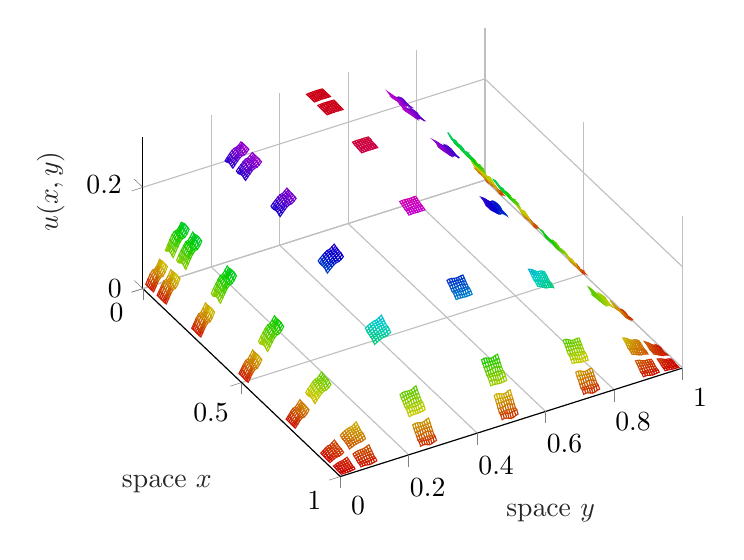
\begin{tikzpicture}

\begin{axis}[%
unbounded coords=jump,
xmin=0,
xmax=1,
tick align=outside,
xlabel style={font=\color{white!15!black}},
xlabel={space $x$},
ymin=0,
ymax=1,
ylabel style={font=\color{white!15!black}},
ylabel={space $y$},
zmin=0,
zmax=0.3,
zlabel style={font=\color{white!15!black}},
zlabel={$u(x,y)$},
view={60}{55},
axis background/.style={fill=white},
axis x line*=bottom,
axis y line*=left,
axis z line*=left,
xmajorgrids,
ymajorgrids,
zmajorgrids,
\extraAxisOptions
]

\addplot3[%
surf,
shader=flat corner, fill=white, z buffer=sort, colormap={mymap}{[1pt] rgb(0pt)=(0.8,0,0); rgb(10pt)=(0.8,0.75,0); rgb(11pt)=(0.775,0.8,0); rgb(21pt)=(0.025,0.8,0); rgb(22pt)=(0,0.8,0.05); rgb(32pt)=(0,0.8,0.8); rgb(42pt)=(0,0.05,0.8); rgb(43pt)=(0.025,0,0.8); rgb(53pt)=(0.775,0,0.8); rgb(54pt)=(0.8,0,0.75); rgb(63pt)=(0.8,0,0.075)}, mesh/rows=63]
table[row sep=crcr, point meta=\thisrow{c}] {%
%
x	y	z	c\\
-0.00333333333333332	-1.73472347597681e-17	nan	nan\\
-0.00333333333333332	0.00666666666666665	nan	nan\\
-0.00333333333333332	0.0133333333333333	nan	nan\\
-0.00333333333333332	0.02	nan	nan\\
-0.00333333333333332	0.0266666666666667	nan	nan\\
-0.00333333333333332	0.0333333333333333	nan	nan\\
-0.00333333333333332	0.04	nan	nan\\
-0.00333333333333332	0.0466666666666666	nan	nan\\
-0.00333333333333332	nan	nan	nan\\
-0.00333333333333332	0.0638612241960842	nan	nan\\
-0.00333333333333332	0.0705278908627509	nan	nan\\
-0.00333333333333332	0.0771945575294175	nan	nan\\
-0.00333333333333332	0.0838612241960842	nan	nan\\
-0.00333333333333332	0.0905278908627508	nan	nan\\
-0.00333333333333332	0.0971945575294175	nan	nan\\
-0.00333333333333332	0.103861224196084	nan	nan\\
-0.00333333333333332	0.110527890862751	nan	nan\\
-0.00333333333333332	nan	nan	nan\\
-0.00333333333333332	0.238333333333333	nan	nan\\
-0.00333333333333332	0.245	nan	nan\\
-0.00333333333333332	0.251666666666667	nan	nan\\
-0.00333333333333332	0.258333333333333	nan	nan\\
-0.00333333333333332	0.265	nan	nan\\
-0.00333333333333332	0.271666666666667	nan	nan\\
-0.00333333333333332	0.278333333333333	nan	nan\\
-0.00333333333333332	0.285	nan	nan\\
-0.00333333333333332	nan	nan	nan\\
-0.00333333333333332	0.476666666666667	nan	nan\\
-0.00333333333333332	0.483333333333333	nan	nan\\
-0.00333333333333332	0.49	nan	nan\\
-0.00333333333333332	0.496666666666667	nan	nan\\
-0.00333333333333332	0.503333333333333	nan	nan\\
-0.00333333333333332	0.51	nan	nan\\
-0.00333333333333332	0.516666666666667	nan	nan\\
-0.00333333333333332	0.523333333333333	nan	nan\\
-0.00333333333333332	nan	nan	nan\\
-0.00333333333333332	0.715	nan	nan\\
-0.00333333333333332	0.721666666666667	nan	nan\\
-0.00333333333333332	0.728333333333333	nan	nan\\
-0.00333333333333332	0.735	nan	nan\\
-0.00333333333333332	0.741666666666667	nan	nan\\
-0.00333333333333332	0.748333333333333	nan	nan\\
-0.00333333333333332	0.755	nan	nan\\
-0.00333333333333332	0.761666666666667	nan	nan\\
-0.00333333333333332	nan	nan	nan\\
-0.00333333333333332	0.889472109137249	nan	nan\\
-0.00333333333333332	0.896138775803916	nan	nan\\
-0.00333333333333332	0.902805442470582	nan	nan\\
-0.00333333333333332	0.909472109137249	nan	nan\\
-0.00333333333333332	0.916138775803916	nan	nan\\
-0.00333333333333332	0.922805442470582	nan	nan\\
-0.00333333333333332	0.929472109137249	nan	nan\\
-0.00333333333333332	0.936138775803916	nan	nan\\
-0.00333333333333332	nan	nan	nan\\
-0.00333333333333332	0.953333333333333	nan	nan\\
-0.00333333333333332	0.96	nan	nan\\
-0.00333333333333332	0.966666666666667	nan	nan\\
-0.00333333333333332	0.973333333333333	nan	nan\\
-0.00333333333333332	0.98	nan	nan\\
-0.00333333333333332	0.986666666666667	nan	nan\\
-0.00333333333333332	0.993333333333333	nan	nan\\
-0.00333333333333332	1	nan	nan\\
-0.00333333333333332	nan	nan	nan\\
0.00333333333333335	-1.73472347597681e-17	nan	nan\\
0.00333333333333335	0.00666666666666665	0.00844161305986431	0.00844161305986431\\
0.00333333333333335	0.0133333333333333	0.0176170618106518	0.0176170618106518\\
0.00333333333333335	0.02	0.0265512984714305	0.0265512984714305\\
0.00333333333333335	0.0266666666666667	0.0319907395318701	0.0319907395318701\\
0.00333333333333335	0.0333333333333333	0.0332270197821145	0.0332270197821145\\
0.00333333333333335	0.04	0.0390615016906748	0.0390615016906748\\
0.00333333333333335	0.0466666666666666	0.0491400740736394	0.0491400740736394\\
0.00333333333333335	nan	nan	nan\\
0.00333333333333335	0.0638612241960842	0.0630190656412216	0.0630190656412216\\
0.00333333333333335	0.0705278908627509	0.0722167836541268	0.0722167836541268\\
0.00333333333333335	0.0771945575294175	0.0814105819293828	0.0814105819293828\\
0.00333333333333335	0.0838612241960842	0.0898631316724031	0.0898631316724031\\
0.00333333333333335	0.0905278908627508	0.094787203108152	0.094787203108152\\
0.00333333333333335	0.0971945575294175	0.0958299378133337	0.0958299378133337\\
0.00333333333333335	0.103861224196084	0.100642969836443	0.100642969836443\\
0.00333333333333335	0.110527890862751	0.108687236093678	0.108687236093678\\
0.00333333333333335	nan	nan	nan\\
0.00333333333333335	0.238333333333333	0.20247123781998	0.20247123781998\\
0.00333333333333335	0.245	0.208090597458545	0.208090597458545\\
0.00333333333333335	0.251666666666667	0.213623315972267	0.213623315972267\\
0.00333333333333335	0.258333333333333	0.218633750392246	0.218633750392246\\
0.00333333333333335	0.265	0.221524581178016	0.221524581178016\\
0.00333333333333335	0.271666666666667	0.222157298475198	0.222157298475198\\
0.00333333333333335	0.278333333333333	0.225085018540384	0.225085018540384\\
0.00333333333333335	0.285	0.230047262170155	0.230047262170155\\
0.00333333333333335	nan	nan	nan\\
0.00333333333333335	0.476666666666667	0.28276343229414	0.28276343229414\\
0.00333333333333335	0.483333333333333	0.283317137150453	0.283317137150453\\
0.00333333333333335	0.49	0.283687641630213	0.283687641630213\\
0.00333333333333335	0.496666666666667	0.283847136822682	0.283847136822682\\
0.00333333333333335	0.503333333333333	0.283854394115486	0.283854394115486\\
0.00333333333333335	0.51	0.283860465603543	0.283860465603543\\
0.00333333333333335	0.516666666666667	0.283808212572191	0.283808212572191\\
0.00333333333333335	0.523333333333333	0.283546530610745	0.283546530610745\\
0.00333333333333335	nan	nan	nan\\
0.00333333333333335	0.715	0.235936453097407	0.235936453097407\\
0.00333333333333335	0.721666666666667	0.231523434536343	0.231523434536343\\
0.00333333333333335	0.728333333333333	0.226790603963261	0.226790603963261\\
0.00333333333333335	0.735	0.222127819150712	0.222127819150712\\
0.00333333333333335	0.741666666666667	0.219259504271718	0.219259504271718\\
0.00333333333333335	0.748333333333333	0.218645723547635	0.218645723547635\\
0.00333333333333335	0.755	0.215661141440929	0.215661141440929\\
0.00333333333333335	0.761666666666667	0.210322056762355	0.210322056762355\\
0.00333333333333335	nan	nan	nan\\
0.00333333333333335	0.889472109137249	0.119383095582504	0.119383095582504\\
0.00333333333333335	0.896138775803916	0.110841476698341	0.110841476698341\\
0.00333333333333335	0.902805442470582	0.101950741493321	0.101950741493321\\
0.00333333333333335	0.909472109137249	0.0934094315727605	0.0934094315727605\\
0.00333333333333335	0.916138775803916	0.0882464843875516	0.0882464843875516\\
0.00333333333333335	0.922805442470582	0.0871376934173261	0.0871376934173261\\
0.00333333333333335	0.929472109137249	0.0818069822763729	0.0818069822763729\\
0.00333333333333335	0.936138775803916	0.0723873732173594	0.0723873732173594\\
0.00333333333333335	nan	nan	nan\\
0.00333333333333335	0.953333333333333	0.0572969994597669	0.0572969994597669\\
0.00333333333333335	0.96	0.0473978636311405	0.0473978636311405\\
0.00333333333333335	0.966666666666667	0.0370005919138869	0.0370005919138869\\
0.00333333333333335	0.973333333333333	0.0269431450185402	0.0269431450185402\\
0.00333333333333335	0.98	0.0208037027658318	0.0208037027658318\\
0.00333333333333335	0.986666666666667	0.0194039468600205	0.0194039468600205\\
0.00333333333333335	0.993333333333333	0.0125481832330879	0.0125481832330879\\
0.00333333333333335	1	nan	nan\\
0.00333333333333335	nan	nan	nan\\
0.01	-1.73472347597681e-17	nan	nan\\
0.01	0.00666666666666665	0.00830271651448654	0.00830271651448654\\
0.01	0.0133333333333333	0.0167991032313737	0.0167991032313737\\
0.01	0.02	0.0255647066198369	0.0255647066198369\\
0.01	0.0266666666666667	0.0318183294863537	0.0318183294863537\\
0.01	0.0333333333333333	0.0334638559575754	0.0334638559575754\\
0.01	0.04	0.0401676061499826	0.0401676061499826\\
0.01	0.0466666666666666	0.0496059399912229	0.0496059399912229\\
0.01	nan	nan	nan\\
0.01	0.0638612241960842	0.0641690808072397	0.0641690808072397\\
0.01	0.0705278908627509	0.0728911763485531	0.0728911763485531\\
0.01	0.0771945575294175	0.0810909931919076	0.0810909931919076\\
0.01	0.0838612241960842	0.0891456102197913	0.0891456102197913\\
0.01	0.0905278908627508	0.0947053542899974	0.0947053542899974\\
0.01	0.0971945575294175	0.0961196541235648	0.0961196541235648\\
0.01	0.103861224196084	0.101785732862697	0.101785732862697\\
0.01	0.110527890862751	0.109515507947386	0.109515507947386\\
0.01	nan	nan	nan\\
0.01	0.238333333333333	0.203177360892633	0.203177360892633\\
0.01	0.245	0.208490238619401	0.208490238619401\\
0.01	0.251666666666667	0.213417281336189	0.213417281336189\\
0.01	0.258333333333333	0.21818942523796	0.21818942523796\\
0.01	0.265	0.221446455157104	0.221446455157104\\
0.01	0.271666666666667	0.222280455911027	0.222280455911027\\
0.01	0.278333333333333	0.225622703256567	0.225622703256567\\
0.01	0.285	0.230249998402512	0.230249998402512\\
0.01	nan	nan	nan\\
0.01	0.476666666666667	0.282797284623698	0.282797284623698\\
0.01	0.483333333333333	0.283307285842886	0.283307285842886\\
0.01	0.49	0.283639191645816	0.283639191645816\\
0.01	0.496666666666667	0.283805971989138	0.283805971989138\\
0.01	0.503333333333333	0.283826700571585	0.283826700571585\\
0.01	0.51	0.28382764084997	0.28382764084997\\
0.01	0.516666666666667	0.283741895277528	0.283741895277528\\
0.01	0.523333333333333	0.283475556311815	0.283475556311815\\
0.01	nan	nan	nan\\
0.01	0.715	0.235374485076809	0.235374485076809\\
0.01	0.721666666666667	0.231154026246989	0.231154026246989\\
0.01	0.728333333333333	0.226924610690103	0.226924610690103\\
0.01	0.735	0.222496467533099	0.222496467533099\\
0.01	0.741666666666667	0.219277048480888	0.219277048480888\\
0.01	0.748333333333333	0.218443270124142	0.218443270124142\\
0.01	0.755	0.214937476581107	0.214937476581107\\
0.01	0.761666666666667	0.209848418068533	0.209848418068533\\
0.01	nan	nan	nan\\
0.01	0.889472109137249	0.118190256200282	0.118190256200282\\
0.01	0.896138775803916	0.110088931407655	0.110088931407655\\
0.01	0.902805442470582	0.102183011486692	0.102183011486692\\
0.01	0.909472109137249	0.0940895200761961	0.0940895200761961\\
0.01	0.916138775803916	0.0883005113489869	0.0883005113489869\\
0.01	0.922805442470582	0.0868041642412915	0.0868041642412915\\
0.01	0.929472109137249	0.0805755217975358	0.0805755217975358\\
0.01	0.936138775803916	0.071624922329745	0.071624922329745\\
0.01	nan	nan	nan\\
0.01	0.953333333333333	0.0560851225298584	0.0560851225298584\\
0.01	0.96	0.046658723892984	0.046658723892984\\
0.01	0.966666666666667	0.0373792939479142	0.0373792939479142\\
0.01	0.973333333333333	0.0278244877656307	0.0278244877656307\\
0.01	0.98	0.0209535654323999	0.0209535654323999\\
0.01	0.986666666666667	0.0191393796408561	0.0191393796408561\\
0.01	0.993333333333333	0.0114627547409629	0.0114627547409629\\
0.01	1	nan	nan\\
0.01	nan	nan	nan\\
0.0166666666666667	-1.73472347597681e-17	nan	nan\\
0.0166666666666667	0.00666666666666665	0.00802111653281571	0.00802111653281571\\
0.0166666666666667	0.0133333333333333	0.0151326285709426	0.0151326285709426\\
0.0166666666666667	0.02	0.023141634180798	0.023141634180798\\
0.0166666666666667	0.0266666666666667	0.0312476454120178	0.0312476454120178\\
0.0166666666666667	0.0333333333333333	0.0346541703303426	0.0346541703303426\\
0.0166666666666667	0.04	0.0430132503831006	0.0430132503831006\\
0.0166666666666667	0.0466666666666666	0.0504704000721744	0.0504704000721744\\
0.0166666666666667	nan	nan	nan\\
0.0166666666666667	0.0638612241960842	0.0670729229775998	0.0670729229775998\\
0.0166666666666667	0.0705278908627509	0.0741501503514408	0.0741501503514408\\
0.0166666666666667	0.0771945575294175	0.0803759821178855	0.0803759821178855\\
0.0166666666666667	0.0838612241960842	0.0873250361688777	0.0873250361688777\\
0.0166666666666667	0.0905278908627508	0.0943360060089848	0.0943360060089848\\
0.0166666666666667	0.0971945575294175	0.0973237422240986	0.0973237422240986\\
0.0166666666666667	0.103861224196084	0.104621281432419	0.104621281432419\\
0.0166666666666667	0.110527890862751	0.11106419068641	0.11106419068641\\
0.0166666666666667	nan	nan	nan\\
0.0166666666666667	0.238333333333333	0.204938477757171	0.204938477757171\\
0.0166666666666667	0.245	0.209217077622329	0.209217077622329\\
0.0166666666666667	0.251666666666667	0.212945237199781	0.212945237199781\\
0.0166666666666667	0.258333333333333	0.217066867971615	0.217066867971615\\
0.0166666666666667	0.265	0.221173052868869	0.221173052868869\\
0.0166666666666667	0.271666666666667	0.222873457472717	0.222873457472717\\
0.0166666666666667	0.278333333333333	0.226985506268211	0.226985506268211\\
0.0166666666666667	0.285	0.23060090286257	0.23060090286257\\
0.0166666666666667	nan	nan	nan\\
0.0166666666666667	0.476666666666667	0.28286728891792	0.28286728891792\\
0.0166666666666667	0.483333333333333	0.283246615751956	0.283246615751956\\
0.0166666666666667	0.49	0.283502937424166	0.283502937424166\\
0.0166666666666667	0.496666666666667	0.283692542194384	0.283692542194384\\
0.0166666666666667	0.503333333333333	0.283764288390856	0.283764288390856\\
0.0166666666666667	0.51	0.283736814558151	0.283736814558151\\
0.0166666666666667	0.516666666666667	0.283554233639297	0.283554233639297\\
0.0166666666666667	0.523333333333333	0.283296494749149	0.283296494749149\\
0.0166666666666667	nan	nan	nan\\
0.0166666666666667	0.715	0.233909612773021	0.233909612773021\\
0.0166666666666667	0.721666666666667	0.230396752029428	0.230396752029428\\
0.0166666666666667	0.728333333333333	0.227172642051081	0.227172642051081\\
0.0166666666666667	0.735	0.223410296422997	0.223410296422997\\
0.0166666666666667	0.741666666666667	0.219419726615412	0.219419726615412\\
0.0166666666666667	0.748333333333333	0.217636208789409	0.217636208789409\\
0.0166666666666667	0.755	0.213085504125706	0.213085504125706\\
0.0166666666666667	0.761666666666667	0.208894959962216	0.208894959962216\\
0.0166666666666667	nan	nan	nan\\
0.0166666666666667	0.889472109137249	0.115186428965476	0.115186428965476\\
0.0166666666666667	0.896138775803916	0.108606807125953	0.108606807125953\\
0.0166666666666667	0.902805442470582	0.102650961218054	0.102650961218054\\
0.0166666666666667	0.909472109137249	0.0957888501904917	0.0957888501904917\\
0.0166666666666667	0.916138775803916	0.0886072210957161	0.0886072210957161\\
0.0166666666666667	0.922805442470582	0.0854410800417185	0.0854410800417185\\
0.0166666666666667	0.929472109137249	0.0774369171868212	0.0774369171868212\\
0.0166666666666667	0.936138775803916	0.070118483285034	0.070118483285034\\
0.0166666666666667	nan	nan	nan\\
0.0166666666666667	0.953333333333333	0.0529541978839113	0.0529541978839113\\
0.0166666666666667	0.96	0.0451908891513861	0.0451908891513861\\
0.0166666666666667	0.966666666666667	0.0381373536452288	0.0381373536452288\\
0.0166666666666667	0.973333333333333	0.0299885379951662	0.0299885379951662\\
0.0166666666666667	0.98	0.0214726340353775	0.0214726340353775\\
0.0166666666666667	0.986666666666667	0.0178123044891771	0.0178123044891771\\
0.0166666666666667	0.993333333333333	0.00853835678733595	0.00853835678733595\\
0.0166666666666667	1	nan	nan\\
0.0166666666666667	nan	nan	nan\\
0.0233333333333334	-1.73472347597681e-17	nan	nan\\
0.0233333333333334	0.00666666666666665	0.00764588258653747	0.00764588258653747\\
0.0233333333333334	0.0133333333333333	0.0138754477132167	0.0138754477132167\\
0.0233333333333334	0.02	0.0206009148520807	0.0206009148520807\\
0.0233333333333334	0.0266666666666667	0.0294393989268279	0.0294393989268279\\
0.0233333333333334	0.0333333333333333	0.0369321177003183	0.0369321177003183\\
0.0233333333333334	0.04	0.0448365749924591	0.0448365749924591\\
0.0233333333333334	0.0466666666666666	0.0508174432798075	0.0508174432798075\\
0.0233333333333334	nan	nan	nan\\
0.0233333333333334	0.0638612241960842	0.0689710147390071	0.0689710147390071\\
0.0233333333333334	0.0705278908627509	0.0747488271183335	0.0747488271183335\\
0.0233333333333334	0.0771945575294175	0.079839322503522	0.079839322503522\\
0.0233333333333334	0.0838612241960842	0.0854939396101267	0.0854939396101267\\
0.0233333333333334	0.0905278908627508	0.0930090400051339	0.0930090400051339\\
0.0233333333333334	0.0971945575294175	0.0995460459112154	0.0995460459112154\\
0.0233333333333334	0.103861224196084	0.106505656617802	0.106505656617802\\
0.0233333333333334	0.110527890862751	0.111854265513114	0.111854265513114\\
0.0233333333333334	nan	nan	nan\\
0.0233333333333334	0.238333333333333	0.206067974320959	0.206067974320959\\
0.0233333333333334	0.245	0.209536045984454	0.209536045984454\\
0.0233333333333334	0.251666666666667	0.212565442056455	0.212565442056455\\
0.0233333333333334	0.258333333333333	0.215899448651614	0.215899448651614\\
0.0233333333333334	0.265	0.22028438174451	0.22028438174451\\
0.0233333333333334	0.271666666666667	0.223975280037764	0.223975280037764\\
0.0233333333333334	0.278333333333333	0.227824260977567	0.227824260977567\\
0.0233333333333334	0.285	0.230697712425188	0.230697712425188\\
0.0233333333333334	nan	nan	nan\\
0.0233333333333334	0.476666666666667	0.282835901637902	0.282835901637902\\
0.0233333333333334	0.483333333333333	0.28314028400437	0.28314028400437\\
0.0233333333333334	0.49	0.283341649855156	0.283341649855156\\
0.0233333333333334	0.496666666666667	0.283494161361712	0.283494161361712\\
0.0233333333333334	0.503333333333333	0.283604315890726	0.283604315890726\\
0.0233333333333334	0.51	0.283535682906299	0.283535682906299\\
0.0233333333333334	0.516666666666667	0.283349898293389	0.283349898293389\\
0.0233333333333334	0.523333333333333	0.283128567671841	0.283128567671841\\
0.0233333333333334	nan	nan	nan\\
0.0233333333333334	0.715	0.232848977026006	0.232848977026006\\
0.0233333333333334	0.721666666666667	0.229934111885666	0.229934111885666\\
0.0233333333333334	0.728333333333333	0.2272740610438	0.2272740610438\\
0.0233333333333334	0.735	0.224210666872625	0.224210666872625\\
0.0233333333333334	0.741666666666667	0.219992672122188	0.219992672122188\\
0.0233333333333334	0.748333333333333	0.216086006721306	0.216086006721306\\
0.0233333333333334	0.755	0.211752312198512	0.211752312198512\\
0.0233333333333334	0.761666666666667	0.208317506279493	0.208317506279493\\
0.0233333333333334	nan	nan	nan\\
0.0233333333333334	0.889472109137249	0.113065821916532	0.113065821916532\\
0.0233333333333334	0.896138775803916	0.107747968227728	0.107747968227728\\
0.0233333333333334	0.902805442470582	0.102899151528147	0.102899151528147\\
0.0233333333333334	0.909472109137249	0.0973503233010307	0.0973503233010307\\
0.0233333333333334	0.916138775803916	0.0897658776255748	0.0897658776255748\\
0.0233333333333334	0.922805442470582	0.0828534446639284	0.0828534446639284\\
0.0233333333333334	0.929472109137249	0.0752503301558249	0.0752503301558249\\
0.0233333333333334	0.936138775803916	0.0692760161631019	0.0692760161631019\\
0.0233333333333334	nan	nan	nan\\
0.0233333333333334	0.953333333333333	0.0507988896367116	0.0507988896367116\\
0.0233333333333334	0.96	0.0443976694402025	0.0443976694402025\\
0.0233333333333334	0.966666666666667	0.0386272986970448	0.0386272986970448\\
0.0233333333333334	0.973333333333333	0.0320606206196525	0.0320606206196525\\
0.0233333333333334	0.98	0.0231252746629874	0.0231252746629874\\
0.0233333333333334	0.986666666666667	0.0152024867565703	0.0152024867565703\\
0.0233333333333334	0.993333333333333	0.0065903935635367	0.0065903935635367\\
0.0233333333333334	1	nan	nan\\
0.0233333333333334	nan	nan	nan\\
0.03	-1.73472347597681e-17	nan	nan\\
0.03	0.00666666666666665	0.00769591076405645	0.00769591076405645\\
0.03	0.0133333333333333	0.0143099026263552	0.0143099026263552\\
0.03	0.02	0.0219270014125689	0.0219270014125689\\
0.03	0.0266666666666667	0.0312570080051763	0.0312570080051763\\
0.03	0.0333333333333333	0.0355230116718562	0.0355230116718562\\
0.03	0.04	0.0440360602245347	0.0440360602245347\\
0.03	0.0466666666666666	0.0506995888421599	0.0506995888421599\\
0.03	nan	nan	nan\\
0.03	0.0638612241960842	0.0681883440288977	0.0681883440288977\\
0.03	0.0705278908627509	0.0745732687470844	0.0745732687470844\\
0.03	0.0771945575294175	0.0801325032133299	0.0801325032133299\\
0.03	0.0838612241960842	0.0866096340348932	0.0866096340348932\\
0.03	0.0905278908627508	0.0946021248750789	0.0946021248750789\\
0.03	0.0971945575294175	0.0983181913795103	0.0983181913795103\\
0.03	0.103861224196084	0.105772817685217	0.105772817685217\\
0.03	0.110527890862751	0.111636399505366	0.111636399505366\\
0.03	nan	nan	nan\\
0.03	0.238333333333333	0.20560131046599	0.20560131046599\\
0.03	0.245	0.209436893380901	0.209436893380901\\
0.03	0.251666666666667	0.212743952658235	0.212743952658235\\
0.03	0.258333333333333	0.216552543511475	0.216552543511475\\
0.03	0.265	0.22118419016631	0.22118419016631\\
0.03	0.271666666666667	0.223290296555441	0.223290296555441\\
0.03	0.278333333333333	0.227444820379009	0.227444820379009\\
0.03	0.285	0.230652139954976	0.230652139954976\\
0.03	nan	nan	nan\\
0.03	0.476666666666667	0.282796732746344	0.282796732746344\\
0.03	0.483333333333333	0.283142241478793	0.283142241478793\\
0.03	0.49	0.283360902748526	0.283360902748526\\
0.03	0.496666666666667	0.283514648726157	0.283514648726157\\
0.03	0.503333333333333	0.28356902626233	0.28356902626233\\
0.03	0.51	0.283548117355786	0.283548117355786\\
0.03	0.516666666666667	0.283379207297691	0.283379207297691\\
0.03	0.523333333333333	0.283146797479805	0.283146797479805\\
0.03	nan	nan	nan\\
0.03	0.715	0.233227582482619	0.233227582482619\\
0.03	0.721666666666667	0.230038001589029	0.230038001589029\\
0.03	0.728333333333333	0.227137809014234	0.227137809014234\\
0.03	0.735	0.223604757363489	0.223604757363489\\
0.03	0.741666666666667	0.219036961961356	0.219036961961356\\
0.03	0.748333333333333	0.21683349936105	0.21683349936105\\
0.03	0.755	0.212221816564646	0.212221816564646\\
0.03	0.761666666666667	0.208444641119712	0.208444641119712\\
0.03	nan	nan	nan\\
0.03	0.889472109137249	0.113832159996181	0.113832159996181\\
0.03	0.896138775803916	0.107954721984192	0.107954721984192\\
0.03	0.902805442470582	0.10265802944642	0.10265802944642\\
0.03	0.909472109137249	0.0962783911641806	0.0962783911641806\\
0.03	0.916138775803916	0.0881315035704048	0.0881315035704048\\
0.03	0.922805442470582	0.0842034469332143	0.0842034469332143\\
0.03	0.929472109137249	0.0760810944520501	0.0760810944520501\\
0.03	0.936138775803916	0.0695027926821251	0.0695027926821251\\
0.03	nan	nan	nan\\
0.03	0.953333333333333	0.0516572796718109	0.0516572796718109\\
0.03	0.96	0.0446345158528797	0.0446345158528797\\
0.03	0.966666666666667	0.0383513805011631	0.0383513805011631\\
0.03	0.973333333333333	0.0308312968231166	0.0308312968231166\\
0.03	0.98	0.0212993586606076	0.0212993586606076\\
0.03	0.986666666666667	0.0167654893962289	0.0167654893962289\\
0.03	0.993333333333333	0.00747092578909089	0.00747092578909089\\
0.03	1	nan	nan\\
0.03	nan	nan	nan\\
0.0366666666666667	-1.73472347597681e-17	nan	nan\\
0.0366666666666667	0.00666666666666665	0.00794973385931363	0.00794973385931363\\
0.0366666666666667	0.0133333333333333	0.0161078062626114	0.0161078062626114\\
0.0366666666666667	0.02	0.0252652480186822	0.0252652480186822\\
0.0366666666666667	0.0266666666666667	0.0320641033695587	0.0320641033695587\\
0.0366666666666667	0.0333333333333333	0.0338097673579084	0.0338097673579084\\
0.0366666666666667	0.04	0.0409982962274166	0.0409982962274166\\
0.0366666666666667	0.0466666666666666	0.0500439085992452	0.0500439085992452\\
0.0366666666666667	nan	nan	nan\\
0.0366666666666667	0.0638612241960842	0.0651771079718788	0.0651771079718788\\
0.0366666666666667	0.0705278908627509	0.0736037474094352	0.0736037474094352\\
0.0366666666666667	0.0771945575294175	0.0812010174013357	0.0812010174013357\\
0.0366666666666667	0.0838612241960842	0.0893225597532685	0.0893225597532685\\
0.0366666666666667	0.0905278908627508	0.0952556963050065	0.0952556963050065\\
0.0366666666666667	0.0971945575294175	0.0967612609101286	0.0967612609101286\\
0.0366666666666667	0.103861224196084	0.102912418792399	0.102912418792399\\
0.0366666666666667	0.110527890862751	0.110434108112258	0.110434108112258\\
0.0366666666666667	nan	nan	nan\\
0.0366666666666667	0.238333333333333	0.203777870351679	0.203777870351679\\
0.0366666666666667	0.245	0.208859648611153	0.208859648611153\\
0.0366666666666667	0.251666666666667	0.213375648882107	0.213375648882107\\
0.0366666666666667	0.258333333333333	0.218128720514667	0.218128720514667\\
0.0366666666666667	0.265	0.221559236684635	0.221559236684635\\
0.0366666666666667	0.271666666666667	0.222432330704512	0.222432330704512\\
0.0366666666666667	0.278333333333333	0.225974340170982	0.225974340170982\\
0.0366666666666667	0.285	0.230359823096908	0.230359823096908\\
0.0366666666666667	nan	nan	nan\\
0.0366666666666667	0.476666666666667	0.282594821350934	0.282594821350934\\
0.0366666666666667	0.483333333333333	0.283089760187136	0.283089760187136\\
0.0366666666666667	0.49	0.283379548786081	0.283379548786081\\
0.0366666666666667	0.496666666666667	0.283511326370184	0.283511326370184\\
0.0366666666666667	0.503333333333333	0.283507606255078	0.283507606255078\\
0.0366666666666667	0.51	0.2835127098824	0.2835127098824\\
0.0366666666666667	0.516666666666667	0.283432395473928	0.283432395473928\\
0.0366666666666667	0.523333333333333	0.28317741349871	0.28317741349871\\
0.0366666666666667	nan	nan	nan\\
0.0366666666666667	0.715	0.234589419880902	0.234589419880902\\
0.0366666666666667	0.721666666666667	0.230505268578509	0.230505268578509\\
0.0366666666666667	0.728333333333333	0.226558499295691	0.226558499295691\\
0.0366666666666667	0.735	0.222051172491819	0.222051172491819\\
0.0366666666666667	0.741666666666667	0.218591794207629	0.218591794207629\\
0.0366666666666667	0.748333333333333	0.217711725459299	0.217711725459299\\
0.0366666666666667	0.755	0.213946381075478	0.213946381075478\\
0.0366666666666667	0.761666666666667	0.209039098879777	0.209039098879777\\
0.0366666666666667	nan	nan	nan\\
0.0366666666666667	0.889472109137249	0.116719236914212	0.116719236914212\\
0.0366666666666667	0.896138775803916	0.108968839435674	0.108968839435674\\
0.0366666666666667	0.902805442470582	0.10170222208777	0.10170222208777\\
0.0366666666666667	0.909472109137249	0.0935954094397817	0.0935954094397817\\
0.0366666666666667	0.916138775803916	0.0874556360378325	0.0874556360378325\\
0.0366666666666667	0.922805442470582	0.0858741959506798	0.0858741959506798\\
0.0366666666666667	0.929472109137249	0.0791900320341964	0.0791900320341964\\
0.0366666666666667	0.936138775803916	0.0706079209401014	0.0706079209401014\\
0.0366666666666667	nan	nan	nan\\
0.0366666666666667	0.953333333333333	0.0548434053628457	0.0548434053628457\\
0.0366666666666667	0.96	0.0457783672324291	0.0457783672324291\\
0.0366666666666667	0.966666666666667	0.0372490085217749	0.0372490085217749\\
0.0366666666666667	0.973333333333333	0.0277422448890522	0.0277422448890522\\
0.0366666666666667	0.98	0.0205391890984444	0.0205391890984444\\
0.0366666666666667	0.986666666666667	0.0186580165042735	0.0186580165042735\\
0.0366666666666667	0.993333333333333	0.0106636189786542	0.0106636189786542\\
0.0366666666666667	1	nan	nan\\
0.0366666666666667	nan	nan	nan\\
0.0433333333333333	-1.73472347597681e-17	nan	nan\\
0.0433333333333333	0.00666666666666665	0.00820503825778415	0.00820503825778415\\
0.0433333333333333	0.0133333333333333	0.0171481319300327	0.0171481319300327\\
0.0433333333333333	0.02	0.0262345642049208	0.0262345642049208\\
0.0433333333333333	0.0266666666666667	0.0320812895929468	0.0320812895929468\\
0.0433333333333333	0.0333333333333333	0.033413512669648	0.033413512669648\\
0.0433333333333333	0.04	0.039562000224924	0.039562000224924\\
0.0433333333333333	0.0466666666666666	0.0495587332440107	0.0495587332440107\\
0.0433333333333333	nan	nan	nan\\
0.0433333333333333	0.0638612241960842	0.0637198025922252	0.0637198025922252\\
0.0433333333333333	0.0705278908627509	0.0728608725362754	0.0728608725362754\\
0.0433333333333333	0.0771945575294175	0.0816970166475756	0.0816970166475756\\
0.0433333333333333	0.0838612241960842	0.0900772605483748	0.0900772605483748\\
0.0433333333333333	0.0905278908627508	0.095262788099791	0.095262788099791\\
0.0433333333333333	0.0971945575294175	0.0963893255287172	0.0963893255287172\\
0.0433333333333333	0.103861224196084	0.10149576244975	0.10149576244975\\
0.0433333333333333	0.110527890862751	0.10949514530838	0.10949514530838\\
0.0433333333333333	nan	nan	nan\\
0.0433333333333333	0.238333333333333	0.202874424154641	0.202874424154641\\
0.0433333333333333	0.245	0.208391607558794	0.208391607558794\\
0.0433333333333333	0.251666666666667	0.213643327584201	0.213643327584201\\
0.0433333333333333	0.258333333333333	0.218545107160176	0.218545107160176\\
0.0433333333333333	0.265	0.221546897409964	0.221546897409964\\
0.0433333333333333	0.271666666666667	0.222216218555887	0.222216218555887\\
0.0433333333333333	0.278333333333333	0.225254610594381	0.225254610594381\\
0.0433333333333333	0.285	0.230110586381665	0.230110586381665\\
0.0433333333333333	nan	nan	nan\\
0.0433333333333333	0.476666666666667	0.282437522182616	0.282437522182616\\
0.0433333333333333	0.483333333333333	0.282977339102331	0.282977339102331\\
0.0433333333333333	0.49	0.283315406352577	0.283315406352577\\
0.0433333333333333	0.496666666666667	0.283449433215684	0.283449433215684\\
0.0433333333333333	0.503333333333333	0.283445255574983	0.283445255574983\\
0.0433333333333333	0.51	0.283449578182003	0.283449578182003\\
0.0433333333333333	0.516666666666667	0.283388426480114	0.283388426480114\\
0.0433333333333333	0.523333333333333	0.283120924056864	0.283120924056864\\
0.0433333333333333	nan	nan	nan\\
0.0433333333333333	0.715	0.235148214668495	0.235148214668495\\
0.0433333333333333	0.721666666666667	0.230758424341302	0.230758424341302\\
0.0433333333333333	0.728333333333333	0.226191855967133	0.226191855967133\\
0.0433333333333333	0.735	0.221543818278477	0.221543818278477\\
0.0433333333333333	0.741666666666667	0.218514824036274	0.218514824036274\\
0.0433333333333333	0.748333333333333	0.217851661436145	0.217851661436145\\
0.0433333333333333	0.755	0.214694180692496	0.214694180692496\\
0.0433333333333333	0.761666666666667	0.209390512547122	0.209390512547122\\
0.0433333333333333	nan	nan	nan\\
0.0433333333333333	0.889472109137249	0.118070753361829	0.118070753361829\\
0.0433333333333333	0.896138775803916	0.10966190502561	0.10966190502561\\
0.0433333333333333	0.902805442470582	0.101193860663917	0.101193860663917\\
0.0433333333333333	0.909472109137249	0.0927966214989082	0.0927966214989082\\
0.0433333333333333	0.916138775803916	0.0874110174214728	0.0874110174214728\\
0.0433333333333333	0.922805442470582	0.0862254149851353	0.0862254149851353\\
0.0433333333333333	0.929472109137249	0.0806410227860956	0.0806410227860956\\
0.0433333333333333	0.936138775803916	0.0713820753012566	0.0713820753012566\\
0.0433333333333333	nan	nan	nan\\
0.0433333333333333	0.953333333333333	0.0563176754875113	0.0563176754875113\\
0.0433333333333333	0.96	0.0465901317465537	0.0465901317465537\\
0.0433333333333333	0.966666666666667	0.0367128045126053	0.0367128045126053\\
0.0433333333333333	0.973333333333333	0.0268757772861214	0.0268757772861214\\
0.0433333333333333	0.98	0.0205320249651375	0.0205320249651375\\
0.0433333333333333	0.986666666666667	0.0190747747078166	0.0190747747078166\\
0.0433333333333333	0.993333333333333	0.0120963907347828	0.0120963907347828\\
0.0433333333333333	1	nan	nan\\
0.0433333333333333	nan	nan	nan\\
nan	-1.73472347597681e-17	nan	nan\\
nan	0.00666666666666665	nan	nan\\
nan	0.0133333333333333	nan	nan\\
nan	0.02	nan	nan\\
nan	0.0266666666666667	nan	nan\\
nan	0.0333333333333333	nan	nan\\
nan	0.04	nan	nan\\
nan	0.0466666666666666	nan	nan\\
nan	nan	nan	nan\\
nan	0.0638612241960842	nan	nan\\
nan	0.0705278908627509	nan	nan\\
nan	0.0771945575294175	nan	nan\\
nan	0.0838612241960842	nan	nan\\
nan	0.0905278908627508	nan	nan\\
nan	0.0971945575294175	nan	nan\\
nan	0.103861224196084	nan	nan\\
nan	0.110527890862751	nan	nan\\
nan	nan	nan	nan\\
nan	0.238333333333333	nan	nan\\
nan	0.245	nan	nan\\
nan	0.251666666666667	nan	nan\\
nan	0.258333333333333	nan	nan\\
nan	0.265	nan	nan\\
nan	0.271666666666667	nan	nan\\
nan	0.278333333333333	nan	nan\\
nan	0.285	nan	nan\\
nan	nan	nan	nan\\
nan	0.476666666666667	nan	nan\\
nan	0.483333333333333	nan	nan\\
nan	0.49	nan	nan\\
nan	0.496666666666667	nan	nan\\
nan	0.503333333333333	nan	nan\\
nan	0.51	nan	nan\\
nan	0.516666666666667	nan	nan\\
nan	0.523333333333333	nan	nan\\
nan	nan	nan	nan\\
nan	0.715	nan	nan\\
nan	0.721666666666667	nan	nan\\
nan	0.728333333333333	nan	nan\\
nan	0.735	nan	nan\\
nan	0.741666666666667	nan	nan\\
nan	0.748333333333333	nan	nan\\
nan	0.755	nan	nan\\
nan	0.761666666666667	nan	nan\\
nan	nan	nan	nan\\
nan	0.889472109137249	nan	nan\\
nan	0.896138775803916	nan	nan\\
nan	0.902805442470582	nan	nan\\
nan	0.909472109137249	nan	nan\\
nan	0.916138775803916	nan	nan\\
nan	0.922805442470582	nan	nan\\
nan	0.929472109137249	nan	nan\\
nan	0.936138775803916	nan	nan\\
nan	nan	nan	nan\\
nan	0.953333333333333	nan	nan\\
nan	0.96	nan	nan\\
nan	0.966666666666667	nan	nan\\
nan	0.973333333333333	nan	nan\\
nan	0.98	nan	nan\\
nan	0.986666666666667	nan	nan\\
nan	0.993333333333333	nan	nan\\
nan	1	nan	nan\\
nan	nan	nan	nan\\
0.0607511818564435	-1.73472347597681e-17	nan	nan\\
0.0607511818564435	0.00666666666666665	0.00791374718261449	0.00791374718261449\\
0.0607511818564435	0.0133333333333333	0.0160463319682357	0.0160463319682357\\
0.0607511818564435	0.02	0.0252266491350259	0.0252266491350259\\
0.0607511818564435	0.0266666666666667	0.0320946141554328	0.0320946141554328\\
0.0607511818564435	0.0333333333333333	0.0338575086996663	0.0338575086996663\\
0.0607511818564435	0.04	0.0411035151153813	0.0411035151153813\\
0.0607511818564435	0.0466666666666666	0.0501712945309911	0.0501712945309911\\
0.0607511818564435	nan	nan	nan\\
0.0607511818564435	0.0638612241960842	0.0653449643280012	0.0653449643280012\\
0.0607511818564435	0.0705278908627509	0.0737813114650266	0.0737813114650266\\
0.0607511818564435	0.0771945575294175	0.0813452699091786	0.0813452699091786\\
0.0607511818564435	0.0838612241960842	0.0894485320799866	0.0894485320799866\\
0.0607511818564435	0.0905278908627508	0.0954113269620952	0.0954113269620952\\
0.0607511818564435	0.0971945575294175	0.0969295276442236	0.0969295276442236\\
0.0607511818564435	0.103861224196084	0.103118861569354	0.103118861569354\\
0.0607511818564435	0.110527890862751	0.110634366368114	0.110634366368114\\
0.0607511818564435	nan	nan	nan\\
0.0607511818564435	0.238333333333333	0.203765442647369	0.203765442647369\\
0.0607511818564435	0.245	0.208829635462941	0.208829635462941\\
0.0607511818564435	0.251666666666667	0.213296150250308	0.213296150250308\\
0.0607511818564435	0.258333333333333	0.217999672101324	0.217999672101324\\
0.0607511818564435	0.265	0.221420271703531	0.221420271703531\\
0.0607511818564435	0.271666666666667	0.222300132416413	0.222300132416413\\
0.0607511818564435	0.278333333333333	0.225860493087849	0.225860493087849\\
0.0607511818564435	0.285	0.230235218104978	0.230235218104978\\
0.0607511818564435	nan	nan	nan\\
0.0607511818564435	0.476666666666667	0.282226636943321	0.282226636943321\\
0.0607511818564435	0.483333333333333	0.282723660666934	0.282723660666934\\
0.0607511818564435	0.49	0.282998778352539	0.282998778352539\\
0.0607511818564435	0.496666666666667	0.283102034758938	0.283102034758938\\
0.0607511818564435	0.503333333333333	0.28307861629383	0.28307861629383\\
0.0607511818564435	0.51	0.283088109184549	0.283088109184549\\
0.0607511818564435	0.516666666666667	0.283020868372413	0.283020868372413\\
0.0607511818564435	0.523333333333333	0.282769499026915	0.282769499026915\\
0.0607511818564435	nan	nan	nan\\
0.0607511818564435	0.715	0.234058142943882	0.234058142943882\\
0.0607511818564435	0.721666666666667	0.229978777849098	0.229978777849098\\
0.0607511818564435	0.728333333333333	0.226042146117498	0.226042146117498\\
0.0607511818564435	0.735	0.221522580778381	0.221522580778381\\
0.0607511818564435	0.741666666666667	0.218029891809068	0.218029891809068\\
0.0607511818564435	0.748333333333333	0.217146275928217	0.217146275928217\\
0.0607511818564435	0.755	0.213368839704982	0.213368839704982\\
0.0607511818564435	0.761666666666667	0.208464608631886	0.208464608631886\\
0.0607511818564435	nan	nan	nan\\
0.0607511818564435	0.889472109137249	0.116137224588021	0.116137224588021\\
0.0607511818564435	0.896138775803916	0.108414680545534	0.108414680545534\\
0.0607511818564435	0.902805442470582	0.101208731842352	0.101208731842352\\
0.0607511818564435	0.909472109137249	0.0931447741283486	0.0931447741283486\\
0.0607511818564435	0.916138775803916	0.0869930895759038	0.0869930895759038\\
0.0607511818564435	0.922805442470582	0.0854075631829389	0.0854075631829389\\
0.0607511818564435	0.929472109137249	0.0787185932749965	0.0787185932749965\\
0.0607511818564435	0.936138775803916	0.0701800342623863	0.0701800342623863\\
0.0607511818564435	nan	nan	nan\\
0.0607511818564435	0.953333333333333	0.0544795905524068	0.0544795905524068\\
0.0607511818564435	0.96	0.0454687376375565	0.0454687376375565\\
0.0607511818564435	0.966666666666667	0.0370303546267765	0.0370303546267765\\
0.0607511818564435	0.973333333333333	0.0275982066027262	0.0275982066027262\\
0.0607511818564435	0.98	0.0204038459566807	0.0204038459566807\\
0.0607511818564435	0.986666666666667	0.0185275937369715	0.0185275937369715\\
0.0607511818564435	0.993333333333333	0.0105684438168156	0.0105684438168156\\
0.0607511818564435	1	nan	nan\\
0.0607511818564435	nan	nan	nan\\
0.0674178485231102	-1.73472347597681e-17	nan	nan\\
0.0674178485231102	0.00666666666666665	0.00811436632944393	0.00811436632944393\\
0.0674178485231102	0.0133333333333333	0.0169680736544234	0.0169680736544234\\
0.0674178485231102	0.02	0.0261078629909848	0.0261078629909848\\
0.0674178485231102	0.0266666666666667	0.0321038698918547	0.0321038698918547\\
0.0674178485231102	0.0333333333333333	0.0334713853148169	0.0334713853148169\\
0.0674178485231102	0.04	0.0397349293184617	0.0397349293184617\\
0.0674178485231102	0.0466666666666666	0.0496982609079573	0.0496982609079573\\
0.0674178485231102	nan	nan	nan\\
0.0674178485231102	0.0638612241960842	0.0639563539997379	0.0639563539997379\\
0.0674178485231102	0.0705278908627509	0.0730721957322633	0.0730721957322633\\
0.0674178485231102	0.0771945575294175	0.0817699882696292	0.0817699882696292\\
0.0674178485231102	0.0838612241960842	0.0901168814402894	0.0901168814402894\\
0.0674178485231102	0.0905278908627508	0.0953953907344462	0.0953953907344462\\
0.0674178485231102	0.0971945575294175	0.0965524663982371	0.0965524663982371\\
0.0674178485231102	0.103861224196084	0.101765092951781	0.101765092951781\\
0.0674178485231102	0.110527890862751	0.109742169229203	0.109742169229203\\
0.0674178485231102	nan	nan	nan\\
0.0674178485231102	0.238333333333333	0.202870629852001	0.202870629852001\\
0.0674178485231102	0.245	0.208343806521767	0.208343806521767\\
0.0674178485231102	0.251666666666667	0.213482956184546	0.213482956184546\\
0.0674178485231102	0.258333333333333	0.218334775526202	0.218334775526202\\
0.0674178485231102	0.265	0.221371968056668	0.221371968056668\\
0.0674178485231102	0.271666666666667	0.22205434656396	0.22205434656396\\
0.0674178485231102	0.278333333333333	0.225131488775763	0.225131488775763\\
0.0674178485231102	0.285	0.229942893429564	0.229942893429564\\
0.0674178485231102	nan	nan	nan\\
0.0674178485231102	0.476666666666667	0.282018782693325	0.282018782693325\\
0.0674178485231102	0.483333333333333	0.282551880112683	0.282551880112683\\
0.0674178485231102	0.49	0.28287394308741	0.28287394308741\\
0.0674178485231102	0.496666666666667	0.282992888430569	0.282992888430569\\
0.0674178485231102	0.503333333333333	0.282981183380519	0.282981183380519\\
0.0674178485231102	0.51	0.282984903926121	0.282984903926121\\
0.0674178485231102	0.516666666666667	0.282920747269429	0.282920747269429\\
0.0674178485231102	0.523333333333333	0.282650062944371	0.282650062944371\\
0.0674178485231102	nan	nan	nan\\
0.0674178485231102	0.715	0.234539813365569	0.234539813365569\\
0.0674178485231102	0.721666666666667	0.230162954945383	0.230162954945383\\
0.0674178485231102	0.728333333333333	0.225660766016422	0.225660766016422\\
0.0674178485231102	0.735	0.221019670269797	0.221019670269797\\
0.0674178485231102	0.741666666666667	0.217932222182459	0.217932222182459\\
0.0674178485231102	0.748333333333333	0.217251552927091	0.217251552927091\\
0.0674178485231102	0.755	0.21403380676736	0.21403380676736\\
0.0674178485231102	0.761666666666667	0.208748798408907	0.208748798408907\\
0.0674178485231102	nan	nan	nan\\
0.0674178485231102	0.889472109137249	0.1173900760458	0.1173900760458\\
0.0674178485231102	0.896138775803916	0.1090426766032	0.1090426766032\\
0.0674178485231102	0.902805442470582	0.100743645482842	0.100743645482842\\
0.0674178485231102	0.909472109137249	0.0924119257696612	0.0924119257696612\\
0.0674178485231102	0.916138775803916	0.0869515594190245	0.0869515594190245\\
0.0674178485231102	0.922805442470582	0.0857393832680431	0.0857393832680431\\
0.0674178485231102	0.929472109137249	0.0800699847623462	0.0800699847623462\\
0.0674178485231102	0.936138775803916	0.0708857614260797	0.0708857614260797\\
0.0674178485231102	nan	nan	nan\\
0.0674178485231102	0.953333333333333	0.0558552731366675	0.0558552731366675\\
0.0674178485231102	0.96	0.0462084880731143	0.0462084880731143\\
0.0674178485231102	0.966666666666667	0.0365415348639274	0.0365415348639274\\
0.0674178485231102	0.973333333333333	0.0268036872547816	0.0268036872547816\\
0.0674178485231102	0.98	0.0203952963251464	0.0203952963251464\\
0.0674178485231102	0.986666666666667	0.018919316659366	0.018919316659366\\
0.0674178485231102	0.993333333333333	0.0119077697419777	0.0119077697419777\\
0.0674178485231102	1	nan	nan\\
0.0674178485231102	nan	nan	nan\\
0.0740845151897768	-1.73472347597681e-17	nan	nan\\
0.0740845151897768	0.00666666666666665	0.00813880774719027	0.00813880774719027\\
0.0740845151897768	0.0133333333333333	0.0165240644041407	0.0165240644041407\\
0.0740845151897768	0.02	0.025391762682581	0.025391762682581\\
0.0740845151897768	0.0266666666666667	0.0319185738487823	0.0319185738487823\\
0.0740845151897768	0.0333333333333333	0.0336195665436679	0.0336195665436679\\
0.0740845151897768	0.04	0.0405006288111761	0.0405006288111761\\
0.0740845151897768	0.0466666666666666	0.0499823500534875	0.0499823500534875\\
0.0740845151897768	nan	nan	nan\\
0.0740845151897768	0.0638612241960842	0.064713140604657	0.064713140604657\\
0.0740845151897768	0.0705278908627509	0.0734401864978719	0.0734401864978719\\
0.0740845151897768	0.0771945575294175	0.0815069084606807	0.0815069084606807\\
0.0740845151897768	0.0838612241960842	0.0895384563266876	0.0895384563266876\\
0.0740845151897768	0.0905278908627508	0.0952577459183774	0.0952577459183774\\
0.0740845151897768	0.0971945575294175	0.0967058751039754	0.0967058751039754\\
0.0740845151897768	0.103861224196084	0.102475788451193	0.102475788451193\\
0.0740845151897768	0.110527890862751	0.110159617515188	0.110159617515188\\
0.0740845151897768	nan	nan	nan\\
0.0740845151897768	0.238333333333333	0.20326874323003	0.20326874323003\\
0.0740845151897768	0.245	0.208488183880528	0.208488183880528\\
0.0740845151897768	0.251666666666667	0.213254443036658	0.213254443036658\\
0.0740845151897768	0.258333333333333	0.217937525042481	0.217937525042481\\
0.0740845151897768	0.265	0.221236203336309	0.221236203336309\\
0.0740845151897768	0.271666666666667	0.222075238756855	0.222075238756855\\
0.0740845151897768	0.278333333333333	0.225422556642059	0.225422556642059\\
0.0740845151897768	0.285	0.229974672034038	0.229974672034038\\
0.0740845151897768	nan	nan	nan\\
0.0740845151897768	0.476666666666667	0.281918691563292	0.281918691563292\\
0.0740845151897768	0.483333333333333	0.282395239676919	0.282395239676919\\
0.0740845151897768	0.49	0.282703899747175	0.282703899747175\\
0.0740845151897768	0.496666666666667	0.282860531320486	0.282860531320486\\
0.0740845151897768	0.503333333333333	0.282876966576918	0.282876966576918\\
0.0740845151897768	0.51	0.282867664791627	0.282867664791627\\
0.0740845151897768	0.516666666666667	0.282745432061817	0.282745432061817\\
0.0740845151897768	0.523333333333333	0.28245036694942	0.28245036694942\\
0.0740845151897768	nan	nan	nan\\
0.0740845151897768	0.715	0.234023683835369	0.234023683835369\\
0.0740845151897768	0.721666666666667	0.229787695160641	0.229787695160641\\
0.0740845151897768	0.728333333333333	0.225621969502513	0.225621969502513\\
0.0740845151897768	0.735	0.22120652210124	0.22120652210124\\
0.0740845151897768	0.741666666666667	0.217897598932228	0.217897598932228\\
0.0740845151897768	0.748333333333333	0.217033780282576	0.217033780282576\\
0.0740845151897768	0.755	0.213429164571189	0.213429164571189\\
0.0740845151897768	0.761666666666667	0.208329208300637	0.208329208300637\\
0.0740845151897768	nan	nan	nan\\
0.0740845151897768	0.889472109137249	0.116551902259451	0.116551902259451\\
0.0740845151897768	0.896138775803916	0.108542911081296	0.108542911081296\\
0.0740845151897768	0.902805442470582	0.100864288959582	0.100864288959582\\
0.0740845151897768	0.909472109137249	0.092896201096783	0.092896201096783\\
0.0740845151897768	0.916138775803916	0.0870175349257331	0.0870175349257331\\
0.0740845151897768	0.922805442470582	0.0854990163163864	0.0854990163163864\\
0.0740845151897768	0.929472109137249	0.0792192631898816	0.0792192631898816\\
0.0740845151897768	0.936138775803916	0.0704077305995638	0.0704077305995638\\
0.0740845151897768	nan	nan	nan\\
0.0740845151897768	0.953333333333333	0.0550193078399567	0.0550193078399567\\
0.0740845151897768	0.96	0.0457597166536072	0.0457597166536072\\
0.0740845151897768	0.966666666666667	0.0368021728558944	0.0368021728558944\\
0.0740845151897768	0.973333333333333	0.0274664716330059	0.0274664716330059\\
0.0740845151897768	0.98	0.0205610511490872	0.0205610511490872\\
0.0740845151897768	0.986666666666667	0.0187500095128619	0.0187500095128619\\
0.0740845151897768	0.993333333333333	0.011144342808275	0.011144342808275\\
0.0740845151897768	1	nan	nan\\
0.0740845151897768	nan	nan	nan\\
0.0807511818564435	-1.73472347597681e-17	nan	nan\\
0.0807511818564435	0.00666666666666665	0.00796115038112948	0.00796115038112948\\
0.0807511818564435	0.0133333333333333	0.0150434809384577	0.0150434809384577\\
0.0807511818564435	0.02	0.0230859459051778	0.0230859459051778\\
0.0807511818564435	0.0266666666666667	0.0313337378053938	0.0313337378053938\\
0.0807511818564435	0.0333333333333333	0.0347854505777142	0.0347854505777142\\
0.0807511818564435	0.04	0.0432433678295157	0.0432433678295157\\
0.0807511818564435	0.0466666666666666	0.0507541912601241	0.0507541912601241\\
0.0807511818564435	nan	nan	nan\\
0.0807511818564435	0.0638612241960842	0.0674474692541987	0.0674474692541987\\
0.0807511818564435	0.0705278908627509	0.0745323732603936	0.0745323732603936\\
0.0807511818564435	0.0771945575294175	0.0807462077315826	0.0807462077315826\\
0.0807511818564435	0.0838612241960842	0.0877144960394389	0.0877144960394389\\
0.0807511818564435	0.0905278908627508	0.094816059009452	0.094816059009452\\
0.0807511818564435	0.0971945575294175	0.0977989953154603	0.0977989953154603\\
0.0807511818564435	0.103861224196084	0.105076434657549	0.105076434657549\\
0.0807511818564435	0.110527890862751	0.111472917628306	0.111472917628306\\
0.0807511818564435	nan	nan	nan\\
0.0807511818564435	0.238333333333333	0.204819231916609	0.204819231916609\\
0.0807511818564435	0.245	0.209024916439956	0.209024916439956\\
0.0807511818564435	0.251666666666667	0.21269248022808	0.21269248022808\\
0.0807511818564435	0.258333333333333	0.216778191382404	0.216778191382404\\
0.0807511818564435	0.265	0.220891820122441	0.220891820122441\\
0.0807511818564435	0.271666666666667	0.22256204454929	0.22256204454929\\
0.0807511818564435	0.278333333333333	0.226608448550363	0.226608448550363\\
0.0807511818564435	0.285	0.23017218237434	0.23017218237434\\
0.0807511818564435	nan	nan	nan\\
0.0807511818564435	0.476666666666667	0.281833189191211	0.281833189191211\\
0.0807511818564435	0.483333333333333	0.282177040995889	0.282177040995889\\
0.0807511818564435	0.49	0.282426826563938	0.282426826563938\\
0.0807511818564435	0.496666666666667	0.28263409337502	0.28263409337502\\
0.0807511818564435	0.503333333333333	0.282724585185596	0.282724585185596\\
0.0807511818564435	0.51	0.282662077657164	0.282662077657164\\
0.0807511818564435	0.516666666666667	0.282409489116037	0.282409489116037\\
0.0807511818564435	0.523333333333333	0.28212026831667	0.28212026831667\\
0.0807511818564435	nan	nan	nan\\
0.0807511818564435	0.715	0.232476439838691	0.232476439838691\\
0.0807511818564435	0.721666666666667	0.228944819691141	0.228944819691141\\
0.0807511818564435	0.728333333333333	0.22573613525408	0.22573613525408\\
0.0807511818564435	0.735	0.221995450999293	0.221995450999293\\
0.0807511818564435	0.741666666666667	0.217983609000695	0.217983609000695\\
0.0807511818564435	0.748333333333333	0.216165435150929	0.216165435150929\\
0.0807511818564435	0.755	0.211546533426849	0.211546533426849\\
0.0807511818564435	0.761666666666667	0.207337787491992	0.207337787491992\\
0.0807511818564435	nan	nan	nan\\
0.0807511818564435	0.889472109137249	0.113700057364748	0.113700057364748\\
0.0807511818564435	0.896138775803916	0.107180763246146	0.107180763246146\\
0.0807511818564435	0.902805442470582	0.101308277163587	0.101308277163587\\
0.0807511818564435	0.909472109137249	0.0945202250224677	0.0945202250224677\\
0.0807511818564435	0.916138775803916	0.087342874371417	0.087342874371417\\
0.0807511818564435	0.922805442470582	0.0841963894303316	0.0841963894303316\\
0.0807511818564435	0.929472109137249	0.0762574782153838	0.0762574782153838\\
0.0807511818564435	0.936138775803916	0.0690416344071861	0.0690416344071861\\
0.0807511818564435	nan	nan	nan\\
0.0807511818564435	0.953333333333333	0.052065065102934	0.052065065102934\\
0.0807511818564435	0.96	0.0444318308039524	0.0444318308039524\\
0.0807511818564435	0.966666666666667	0.0375270805912244	0.0375270805912244\\
0.0807511818564435	0.973333333333333	0.0295276203348205	0.0295276203348205\\
0.0807511818564435	0.98	0.0210902690886763	0.0210902690886763\\
0.0807511818564435	0.986666666666667	0.0174830507147886	0.0174830507147886\\
0.0807511818564435	0.993333333333333	0.00836206920906673	0.00836206920906673\\
0.0807511818564435	1	nan	nan\\
0.0807511818564435	nan	nan	nan\\
0.0874178485231102	-1.73472347597681e-17	nan	nan\\
0.0874178485231102	0.00666666666666665	0.00762431943366654	0.00762431943366654\\
0.0874178485231102	0.0133333333333333	0.0138501655489426	0.0138501655489426\\
0.0874178485231102	0.02	0.0205974323948818	0.0205974323948818\\
0.0874178485231102	0.0266666666666667	0.0294998123803557	0.0294998123803557\\
0.0874178485231102	0.0333333333333333	0.0370544939671354	0.0370544939671354\\
0.0874178485231102	0.04	0.0450288550454492	0.0450288550454492\\
0.0874178485231102	0.0466666666666666	0.0510543284829675	0.0510543284829675\\
0.0874178485231102	nan	nan	nan\\
0.0874178485231102	0.0638612241960842	0.0692597161910017	0.0692597161910017\\
0.0874178485231102	0.0705278908627509	0.0750504095042283	0.0750504095042283\\
0.0874178485231102	0.0771945575294175	0.080144586723843	0.080144586723843\\
0.0874178485231102	0.0838612241960842	0.0858098695172991	0.0858098695172991\\
0.0874178485231102	0.0905278908627508	0.0933597513874232	0.0933597513874232\\
0.0874178485231102	0.0971945575294175	0.0998803284304136	0.0998803284304136\\
0.0874178485231102	0.103861224196084	0.106824390614374	0.106824390614374\\
0.0874178485231102	0.110527890862751	0.112148133541395	0.112148133541395\\
0.0874178485231102	nan	nan	nan\\
0.0874178485231102	0.238333333333333	0.20580229938655	0.20580229938655\\
0.0874178485231102	0.245	0.209227098329961	0.209227098329961\\
0.0874178485231102	0.251666666666667	0.212216541379876	0.212216541379876\\
0.0874178485231102	0.258333333333333	0.215513958128764	0.215513958128764\\
0.0874178485231102	0.265	0.21987166739182	0.21987166739182\\
0.0874178485231102	0.271666666666667	0.223505988943581	0.223505988943581\\
0.0874178485231102	0.278333333333333	0.227316145734145	0.227316145734145\\
0.0874178485231102	0.285	0.230162331192967	0.230162331192967\\
0.0874178485231102	nan	nan	nan\\
0.0874178485231102	0.476666666666667	0.281664597280914	0.281664597280914\\
0.0874178485231102	0.483333333333333	0.281952189793091	0.281952189793091\\
0.0874178485231102	0.49	0.282141569115504	0.282141569115504\\
0.0874178485231102	0.496666666666667	0.282286006566114	0.282286006566114\\
0.0874178485231102	0.503333333333333	0.282398171691185	0.282398171691185\\
0.0874178485231102	0.51	0.282282842488836	0.282282842488836\\
0.0874178485231102	0.516666666666667	0.282070128771692	0.282070128771692\\
0.0874178485231102	0.523333333333333	0.281835506814015	0.281835506814015\\
0.0874178485231102	nan	nan	nan\\
0.0874178485231102	0.715	0.231317130950752	0.231317130950752\\
0.0874178485231102	0.721666666666667	0.228399253822893	0.228399253822893\\
0.0874178485231102	0.728333333333333	0.225739448991568	0.225739448991568\\
0.0874178485231102	0.735	0.222674754289822	0.222674754289822\\
0.0874178485231102	0.741666666666667	0.218452110086706	0.218452110086706\\
0.0874178485231102	0.748333333333333	0.214507693087131	0.214507693087131\\
0.0874178485231102	0.755	0.210149236125924	0.210149236125924\\
0.0874178485231102	0.761666666666667	0.206706578388295	0.206706578388295\\
0.0874178485231102	nan	nan	nan\\
0.0874178485231102	0.889472109137249	0.111640775659061	0.111640775659061\\
0.0874178485231102	0.896138775803916	0.10636309137098	0.10636309137098\\
0.0874178485231102	0.902805442470582	0.101560408022888	0.101560408022888\\
0.0874178485231102	0.909472109137249	0.0960600401033253	0.0960600401033253\\
0.0874178485231102	0.916138775803916	0.0885266030280151	0.0885266030280151\\
0.0874178485231102	0.922805442470582	0.0816774639248577	0.0816774639248577\\
0.0874178485231102	0.929472109137249	0.0741506067650709	0.0741506067650709\\
0.0874178485231102	0.936138775803916	0.0682504682705961	0.0682504682705961\\
0.0874178485231102	nan	nan	nan\\
0.0874178485231102	0.953333333333333	0.0499905653364854	0.0499905653364854\\
0.0874178485231102	0.96	0.0436875686742854	0.0436875686742854\\
0.0874178485231102	0.966666666666667	0.0380136396194667	0.0380136396194667\\
0.0874178485231102	0.973333333333333	0.031551436354612	0.031551436354612\\
0.0874178485231102	0.98	0.0227422763769944	0.0227422763769944\\
0.0874178485231102	0.986666666666667	0.0149444880639418	0.0149444880639418\\
0.0874178485231102	0.993333333333333	0.00647393942165376	0.00647393942165376\\
0.0874178485231102	1	nan	nan\\
0.0874178485231102	nan	nan	nan\\
0.0940845151897768	-1.73472347597681e-17	nan	nan\\
0.0940845151897768	0.00666666666666665	0.00766775783271378	0.00766775783271378\\
0.0940845151897768	0.0133333333333333	0.0142718423976791	0.0142718423976791\\
0.0940845151897768	0.02	0.0219113549820472	0.0219113549820472\\
0.0940845151897768	0.0266666666666667	0.0313098349968862	0.0313098349968862\\
0.0940845151897768	0.0333333333333333	0.0356211414564374	0.0356211414564374\\
0.0940845151897768	0.04	0.0442184748188822	0.0442184748188822\\
0.0940845151897768	0.0466666666666666	0.0509285084214678	0.0509285084214678\\
0.0940845151897768	nan	nan	nan\\
0.0940845151897768	0.0638612241960842	0.0684659229186998	0.0684659229186998\\
0.0940845151897768	0.0705278908627509	0.0748657634667483	0.0748657634667483\\
0.0940845151897768	0.0771945575294175	0.0804178043418852	0.0804178043418852\\
0.0940845151897768	0.0838612241960842	0.0868856090244005	0.0868856090244005\\
0.0940845151897768	0.0905278908627508	0.0948756355835778	0.0948756355835778\\
0.0940845151897768	0.0971945575294175	0.0986118148492613	0.0986118148492613\\
0.0940845151897768	0.103861224196084	0.106078130501541	0.106078130501541\\
0.0940845151897768	0.110527890862751	0.111918955901746	0.111918955901746\\
0.0940845151897768	nan	nan	nan\\
0.0940845151897768	0.238333333333333	0.205313859584827	0.205313859584827\\
0.0940845151897768	0.245	0.209108360421755	0.209108360421755\\
0.0940845151897768	0.251666666666667	0.212363507752548	0.212363507752548\\
0.0940845151897768	0.258333333333333	0.216104619730284	0.216104619730284\\
0.0940845151897768	0.265	0.220652751542037	0.220652751542037\\
0.0940845151897768	0.271666666666667	0.222767061594187	0.222767061594187\\
0.0940845151897768	0.278333333333333	0.226912589843844	0.226912589843844\\
0.0940845151897768	0.285	0.23009507478741	0.23009507478741\\
0.0940845151897768	nan	nan	nan\\
0.0940845151897768	0.476666666666667	0.281593717391656	0.281593717391656\\
0.0940845151897768	0.483333333333333	0.281928361381287	0.281928361381287\\
0.0940845151897768	0.49	0.282128383456326	0.282128383456326\\
0.0940845151897768	0.496666666666667	0.282245209213549	0.282245209213549\\
0.0940845151897768	0.503333333333333	0.282234363209043	0.282234363209043\\
0.0940845151897768	0.51	0.28223093217497	0.28223093217497\\
0.0940845151897768	0.516666666666667	0.282067780635104	0.282067780635104\\
0.0940845151897768	0.523333333333333	0.281828041345637	0.281828041345637\\
0.0940845151897768	nan	nan	nan\\
0.0940845151897768	0.715	0.231671206389765	0.231671206389765\\
0.0940845151897768	0.721666666666667	0.228483763090782	0.228483763090782\\
0.0940845151897768	0.728333333333333	0.225584092016801	0.225584092016801\\
0.0940845151897768	0.735	0.222034114875976	0.222034114875976\\
0.0940845151897768	0.741666666666667	0.217416633184943	0.217416633184943\\
0.0940845151897768	0.748333333333333	0.215217372480057	0.215217372480057\\
0.0940845151897768	0.755	0.210597932003521	0.210597932003521\\
0.0940845151897768	0.761666666666667	0.206818174338668	0.206818174338668\\
0.0940845151897768	nan	nan	nan\\
0.0940845151897768	0.889472109137249	0.112396487694844	0.112396487694844\\
0.0940845151897768	0.896138775803916	0.106565503689768	0.106565503689768\\
0.0940845151897768	0.902805442470582	0.101326906528033	0.101326906528033\\
0.0940845151897768	0.909472109137249	0.0950097259522332	0.0950097259522332\\
0.0940845151897768	0.916138775803916	0.0869210231696206	0.0869210231696206\\
0.0940845151897768	0.922805442470582	0.0830217869681995	0.0830217869681995\\
0.0940845151897768	0.929472109137249	0.0749706219287563	0.0749706219287563\\
0.0940845151897768	0.936138775803916	0.0684734688936724	0.0684734688936724\\
0.0940845151897768	nan	nan	nan\\
0.0940845151897768	0.953333333333333	0.050836819930651	0.050836819930651\\
0.0940845151897768	0.96	0.0439198019149075	0.0439198019149075\\
0.0940845151897768	0.966666666666667	0.0377480310250512	0.0377480310250512\\
0.0940845151897768	0.973333333333333	0.0303520166589833	0.0303520166589833\\
0.0940845151897768	0.98	0.0209522405510902	0.0209522405510902\\
0.0940845151897768	0.986666666666667	0.0164855036118823	0.0164855036118823\\
0.0940845151897768	0.993333333333333	0.00733715056650091	0.00733715056650091\\
0.0940845151897768	1	nan	nan\\
0.0940845151897768	nan	nan	nan\\
0.100751181856443	-1.73472347597681e-17	nan	nan\\
0.100751181856443	0.00666666666666665	0.00787385787897327	0.00787385787897327\\
0.100751181856443	0.0133333333333333	0.0159755026156941	0.0159755026156941\\
0.100751181856443	0.02	0.0251667438908769	0.0251667438908769\\
0.100751181856443	0.0266666666666667	0.0320897779584405	0.0320897779584405\\
0.100751181856443	0.0333333333333333	0.0338676515307418	0.0338676515307418\\
0.100751181856443	0.04	0.0411625689457119	0.0411625689457119\\
0.100751181856443	0.0466666666666666	0.0502441067267656	0.0502441067267656\\
0.100751181856443	nan	nan	nan\\
0.100751181856443	0.0638612241960842	0.0654336250666411	0.0654336250666411\\
0.100751181856443	0.0705278908627509	0.0738712036607194	0.0738712036607194\\
0.100751181856443	0.0771945575294175	0.0813928495010351	0.0813928495010351\\
0.100751181856443	0.0838612241960842	0.0894606814649342	0.0894606814649342\\
0.100751181856443	0.0905278908627508	0.0954359124681911	0.0954359124681911\\
0.100751181856443	0.0971945575294175	0.0969655896483062	0.0969655896483062\\
0.100751181856443	0.103861224196084	0.103187298365684	0.103187298365684\\
0.100751181856443	0.110527890862751	0.11068819737638	0.11068819737638\\
0.100751181856443	nan	nan	nan\\
0.100751181856443	0.238333333333333	0.20340860068157	0.20340860068157\\
0.100751181856443	0.245	0.208449187515074	0.208449187515074\\
0.100751181856443	0.251666666666667	0.212854132451775	0.212854132451775\\
0.100751181856443	0.258333333333333	0.217485691114701	0.217485691114701\\
0.100751181856443	0.265	0.220877648470468	0.220877648470468\\
0.100751181856443	0.271666666666667	0.221765018296987	0.221765018296987\\
0.100751181856443	0.278333333333333	0.225344635846256	0.225344635846256\\
0.100751181856443	0.285	0.229704021487846	0.229704021487846\\
0.100751181856443	nan	nan	nan\\
0.100751181856443	0.476666666666667	0.28125517851417	0.28125517851417\\
0.100751181856443	0.483333333333333	0.281756304434583	0.281756304434583\\
0.100751181856443	0.49	0.282009009219835	0.282009009219835\\
0.100751181856443	0.496666666666667	0.282066509993083	0.282066509993083\\
0.100751181856443	0.503333333333333	0.282011095734926	0.282011095734926\\
0.100751181856443	0.51	0.282028037625882	0.282028037625882\\
0.100751181856443	0.516666666666667	0.281983395938179	0.281983395938179\\
0.100751181856443	0.523333333333333	0.281738630870093	0.281738630870093\\
0.100751181856443	nan	nan	nan\\
0.100751181856443	0.715	0.232918261535299	0.232918261535299\\
0.100751181856443	0.721666666666667	0.228855685371025	0.228855685371025\\
0.100751181856443	0.728333333333333	0.224931755760452	0.224931755760452\\
0.100751181856443	0.735	0.220398353433655	0.220398353433655\\
0.100751181856443	0.741666666666667	0.216874264267531	0.216874264267531\\
0.100751181856443	0.748333333333333	0.215991856807322	0.215991856807322\\
0.100751181856443	0.755	0.212219545725277	0.212219545725277\\
0.100751181856443	0.761666666666667	0.207332010858897	0.207332010858897\\
0.100751181856443	nan	nan	nan\\
0.100751181856443	0.889472109137249	0.115214031085791	0.115214031085791\\
0.100751181856443	0.896138775803916	0.10754070129543	0.10754070129543\\
0.100751181856443	0.902805442470582	0.100410842845378	0.100410842845378\\
0.100751181856443	0.909472109137249	0.0924088964110326	0.0924088964110326\\
0.100751181856443	0.916138775803916	0.0862647496988308	0.0862647496988308\\
0.100751181856443	0.922805442470582	0.0846810387796931	0.0846810387796931\\
0.100751181856443	0.929472109137249	0.0780109127667702	0.0780109127667702\\
0.100751181856443	0.936138775803916	0.0695410049149745	0.0695410049149745\\
0.100751181856443	nan	nan	nan\\
0.100751181856443	0.953333333333333	0.0539510519870243	0.0539510519870243\\
0.100751181856443	0.96	0.0450222322218704	0.0450222322218704\\
0.100751181856443	0.966666666666667	0.0366971299910802	0.0366971299910802\\
0.100751181856443	0.973333333333333	0.0273671987408696	0.0273671987408696\\
0.100751181856443	0.98	0.0202072692320883	0.0202072692320883\\
0.100751181856443	0.986666666666667	0.018342393991799	0.018342393991799\\
0.100751181856443	0.993333333333333	0.0104442882621618	0.0104442882621618\\
0.100751181856443	1	nan	nan\\
0.100751181856443	nan	nan	nan\\
0.10741784852311	-1.73472347597681e-17	nan	nan\\
0.10741784852311	0.00666666666666665	0.00802690714804806	0.00802690714804806\\
0.10741784852311	0.0133333333333333	0.0167933280422246	0.0167933280422246\\
0.10741784852311	0.02	0.0259697364405483	0.0259697364405483\\
0.10741784852311	0.0266666666666667	0.0320894121211385	0.0320894121211385\\
0.10741784852311	0.0333333333333333	0.0334864628631676	0.0334864628631676\\
0.10741784852311	0.04	0.0398446890316281	0.0398446890316281\\
0.10741784852311	0.0466666666666666	0.0497690890304286	0.0497690890304286\\
0.10741784852311	nan	nan	nan\\
0.10741784852311	0.0638612241960842	0.0640910105073964	0.0640910105073964\\
0.10741784852311	0.0705278908627509	0.073173265356694	0.073173265356694\\
0.10741784852311	0.0771945575294175	0.0817364290526028	0.0817364290526028\\
0.10741784852311	0.0838612241960842	0.0900382526773241	0.0900382526773241\\
0.10741784852311	0.0905278908627508	0.0953875552547302	0.0953875552547302\\
0.10741784852311	0.0971945575294175	0.0965696808386196	0.0965696808386196\\
0.10741784852311	0.103861224196084	0.101867573100725	0.101867573100725\\
0.10741784852311	0.110527890862751	0.10981146048629	0.10981146048629\\
0.10741784852311	nan	nan	nan\\
0.10741784852311	0.238333333333333	0.202490796301973	0.202490796301973\\
0.10741784852311	0.245	0.207912044718058	0.207912044718058\\
0.10741784852311	0.251666666666667	0.212935191296862	0.212935191296862\\
0.10741784852311	0.258333333333333	0.217722656116639	0.217722656116639\\
0.10741784852311	0.265	0.2207780166003	0.2207780166003\\
0.10741784852311	0.271666666666667	0.221470511472982	0.221470511472982\\
0.10741784852311	0.278333333333333	0.22457587039798	0.22457587039798\\
0.10741784852311	0.285	0.229336822088817	0.229336822088817\\
0.10741784852311	nan	nan	nan\\
0.10741784852311	0.476666666666667	0.280962461356364	0.280962461356364\\
0.10741784852311	0.483333333333333	0.281486707732303	0.281486707732303\\
0.10741784852311	0.49	0.281786768568203	0.281786768568203\\
0.10741784852311	0.496666666666667	0.281881008216749	0.281881008216749\\
0.10741784852311	0.503333333333333	0.281856049130145	0.281856049130145\\
0.10741784852311	0.51	0.281859426884991	0.281859426884991\\
0.10741784852311	0.516666666666667	0.281793688330835	0.281793688330835\\
0.10741784852311	0.523333333333333	0.281518738364196	0.281518738364196\\
0.10741784852311	nan	nan	nan\\
0.10741784852311	0.715	0.233303346508859	0.233303346508859\\
0.10741784852311	0.721666666666667	0.228948345243206	0.228948345243206\\
0.10741784852311	0.728333333333333	0.224509229872261	0.224509229872261\\
0.10741784852311	0.735	0.21987872203576	0.21987872203576\\
0.10741784852311	0.741666666666667	0.216743920227254	0.216743920227254\\
0.10741784852311	0.748333333333333	0.216049995799068	0.216049995799068\\
0.10741784852311	0.755	0.212789172312687	0.212789172312687\\
0.10741784852311	0.761666666666667	0.207533700073227	0.207533700073227\\
0.10741784852311	nan	nan	nan\\
0.10741784852311	0.889472109137249	0.116378348898071	0.116378348898071\\
0.10741784852311	0.896138775803916	0.108111523705735	0.108111523705735\\
0.10741784852311	0.902805442470582	0.0999862468239976	0.0999862468239976\\
0.10741784852311	0.909472109137249	0.0917379741035087	0.0917379741035087\\
0.10741784852311	0.916138775803916	0.0862299323778076	0.0862299323778076\\
0.10741784852311	0.922805442470582	0.0849989133318917	0.0849989133318917\\
0.10741784852311	0.929472109137249	0.0792757053023736	0.0792757053023736\\
0.10741784852311	0.936138775803916	0.0701894041911168	0.0701894041911168\\
0.10741784852311	nan	nan	nan\\
0.10741784852311	0.953333333333333	0.0552410711474661	0.0552410711474661\\
0.10741784852311	0.96	0.0457013291569291	0.0457013291569291\\
0.10741784852311	0.966666666666667	0.0362545898295061	0.0362545898295061\\
0.10741784852311	0.973333333333333	0.026640140525336	0.026640140525336\\
0.10741784852311	0.98	0.020199531078795	0.020199531078795\\
0.10741784852311	0.986666666666667	0.0187128663897155	0.0187128663897155\\
0.10741784852311	0.993333333333333	0.0116989575828024	0.0116989575828024\\
0.10741784852311	1	nan	nan\\
0.10741784852311	nan	nan	nan\\
nan	-1.73472347597681e-17	nan	nan\\
nan	0.00666666666666665	nan	nan\\
nan	0.0133333333333333	nan	nan\\
nan	0.02	nan	nan\\
nan	0.0266666666666667	nan	nan\\
nan	0.0333333333333333	nan	nan\\
nan	0.04	nan	nan\\
nan	0.0466666666666666	nan	nan\\
nan	nan	nan	nan\\
nan	0.0638612241960842	nan	nan\\
nan	0.0705278908627509	nan	nan\\
nan	0.0771945575294175	nan	nan\\
nan	0.0838612241960842	nan	nan\\
nan	0.0905278908627508	nan	nan\\
nan	0.0971945575294175	nan	nan\\
nan	0.103861224196084	nan	nan\\
nan	0.110527890862751	nan	nan\\
nan	nan	nan	nan\\
nan	0.238333333333333	nan	nan\\
nan	0.245	nan	nan\\
nan	0.251666666666667	nan	nan\\
nan	0.258333333333333	nan	nan\\
nan	0.265	nan	nan\\
nan	0.271666666666667	nan	nan\\
nan	0.278333333333333	nan	nan\\
nan	0.285	nan	nan\\
nan	nan	nan	nan\\
nan	0.476666666666667	nan	nan\\
nan	0.483333333333333	nan	nan\\
nan	0.49	nan	nan\\
nan	0.496666666666667	nan	nan\\
nan	0.503333333333333	nan	nan\\
nan	0.51	nan	nan\\
nan	0.516666666666667	nan	nan\\
nan	0.523333333333333	nan	nan\\
nan	nan	nan	nan\\
nan	0.715	nan	nan\\
nan	0.721666666666667	nan	nan\\
nan	0.728333333333333	nan	nan\\
nan	0.735	nan	nan\\
nan	0.741666666666667	nan	nan\\
nan	0.748333333333333	nan	nan\\
nan	0.755	nan	nan\\
nan	0.761666666666667	nan	nan\\
nan	nan	nan	nan\\
nan	0.889472109137249	nan	nan\\
nan	0.896138775803916	nan	nan\\
nan	0.902805442470582	nan	nan\\
nan	0.909472109137249	nan	nan\\
nan	0.916138775803916	nan	nan\\
nan	0.922805442470582	nan	nan\\
nan	0.929472109137249	nan	nan\\
nan	0.936138775803916	nan	nan\\
nan	nan	nan	nan\\
nan	0.953333333333333	nan	nan\\
nan	0.96	nan	nan\\
nan	0.966666666666667	nan	nan\\
nan	0.973333333333333	nan	nan\\
nan	0.98	nan	nan\\
nan	0.986666666666667	nan	nan\\
nan	0.993333333333333	nan	nan\\
nan	1	nan	nan\\
nan	nan	nan	nan\\
0.235833333333333	-1.73472347597681e-17	nan	nan\\
0.235833333333333	0.00666666666666665	0.00779308596778382	0.00779308596778382\\
0.235833333333333	0.0133333333333333	0.0157982515317531	0.0157982515317531\\
0.235833333333333	0.02	0.0248315239636504	0.0248315239636504\\
0.235833333333333	0.0266666666666667	0.0315940478231206	0.0315940478231206\\
0.235833333333333	0.0333333333333333	0.0333417916916869	0.0333417916916869\\
0.235833333333333	0.04	0.0405179713652335	0.0405179713652335\\
0.235833333333333	0.0466666666666666	0.0494694727436321	0.0494694727436321\\
0.235833333333333	nan	nan	nan\\
0.235833333333333	0.0638612241960842	0.0643624349517881	0.0643624349517881\\
0.235833333333333	0.0705278908627509	0.0726765190202192	0.0726765190202192\\
0.235833333333333	0.0771945575294175	0.0800769735510937	0.0800769735510937\\
0.235833333333333	0.0838612241960842	0.0879546971106411	0.0879546971106411\\
0.235833333333333	0.0905278908627508	0.0937527195967457	0.0937527195967457\\
0.235833333333333	0.0971945575294175	0.0952636095156456	0.0952636095156456\\
0.235833333333333	0.103861224196084	0.101400491085008	0.101400491085008\\
0.235833333333333	0.110527890862751	0.108788277471267	0.108788277471267\\
0.235833333333333	nan	nan	nan\\
0.235833333333333	0.238333333333333	0.19934905793714	0.19934905793714\\
0.235833333333333	0.245	0.204314959233655	0.204314959233655\\
0.235833333333333	0.251666666666667	0.208594554976576	0.208594554976576\\
0.235833333333333	0.258333333333333	0.213010431684554	0.213010431684554\\
0.235833333333333	0.265	0.216225518457115	0.216225518457115\\
0.235833333333333	0.271666666666667	0.217116007376932	0.217116007376932\\
0.235833333333333	0.278333333333333	0.220688999571926	0.220688999571926\\
0.235833333333333	0.285	0.224988034579453	0.224988034579453\\
0.235833333333333	nan	nan	nan\\
0.235833333333333	0.476666666666667	0.274590838938026	0.274590838938026\\
0.235833333333333	0.483333333333333	0.275114872587576	0.275114872587576\\
0.235833333333333	0.49	0.275300651395561	0.275300651395561\\
0.235833333333333	0.496666666666667	0.275205150390017	0.275205150390017\\
0.235833333333333	0.503333333333333	0.275041651426724	0.275041651426724\\
0.235833333333333	0.51	0.275088751240284	0.275088751240284\\
0.235833333333333	0.516666666666667	0.275140342790584	0.275140342790584\\
0.235833333333333	0.523333333333333	0.274934240992863	0.274934240992863\\
0.235833333333333	nan	nan	nan\\
0.235833333333333	0.715	0.226644985594677	0.226644985594677\\
0.235833333333333	0.721666666666667	0.222717991779315	0.222717991779315\\
0.235833333333333	0.728333333333333	0.218843182551566	0.218843182551566\\
0.235833333333333	0.735	0.214322342298337	0.214322342298337\\
0.235833333333333	0.741666666666667	0.210834019475817	0.210834019475817\\
0.235833333333333	0.748333333333333	0.210000096591049	0.210000096591049\\
0.235833333333333	0.755	0.206406408671541	0.206406408671541\\
0.235833333333333	0.761666666666667	0.201672162278354	0.201672162278354\\
0.235833333333333	nan	nan	nan\\
0.235833333333333	0.889472109137249	0.111913161381981	0.111913161381981\\
0.235833333333333	0.896138775803916	0.104460218707344	0.104460218707344\\
0.235833333333333	0.902805442470582	0.0974931745151319	0.0974931745151319\\
0.235833333333333	0.909472109137249	0.0896836045049666	0.0896836045049666\\
0.235833333333333	0.916138775803916	0.0837252396360654	0.0837252396360654\\
0.235833333333333	0.922805442470582	0.0821991246361861	0.0821991246361861\\
0.235833333333333	0.929472109137249	0.0757594185439005	0.0757594185439005\\
0.235833333333333	0.936138775803916	0.0675371800867709	0.0675371800867709\\
0.235833333333333	nan	nan	nan\\
0.235833333333333	0.953333333333333	0.0523939417643968	0.0523939417643968\\
0.235833333333333	0.96	0.0437320162298447	0.0437320162298447\\
0.235833333333333	0.966666666666667	0.0356223551237744	0.0356223551237744\\
0.235833333333333	0.973333333333333	0.0265522963510004	0.0265522963510004\\
0.235833333333333	0.98	0.0196284762716879	0.0196284762716879\\
0.235833333333333	0.986666666666667	0.0178238685106314	0.0178238685106314\\
0.235833333333333	0.993333333333333	0.0101675208176594	0.0101675208176594\\
0.235833333333333	1	nan	nan\\
0.235833333333333	nan	nan	nan\\
0.2425	-1.73472347597681e-17	nan	nan\\
0.2425	0.00666666666666665	0.00798291999064232	0.00798291999064232\\
0.2425	0.0133333333333333	0.0166894385783269	0.0166894385783269\\
0.2425	0.02	0.0256739156592438	0.0256739156592438\\
0.2425	0.0266666666666667	0.0315680213925162	0.0315680213925162\\
0.2425	0.0333333333333333	0.0329148054367299	0.0329148054367299\\
0.2425	0.04	0.0390828458463323	0.0390828458463323\\
0.2425	0.0466666666666666	0.0488840603938166	0.0488840603938166\\
0.2425	nan	nan	nan\\
0.2425	0.0638612241960842	0.0628574232446877	0.0628574232446877\\
0.2425	0.0705278908627509	0.0718061387503098	0.0718061387503098\\
0.2425	0.0771945575294175	0.0803172929568708	0.0803172929568708\\
0.2425	0.0838612241960842	0.0884627072079279	0.0884627072079279\\
0.2425	0.0905278908627508	0.0936131085908754	0.0936131085908754\\
0.2425	0.0971945575294175	0.0947489820385237	0.0947489820385237\\
0.2425	0.103861224196084	0.0998642680189928	0.0998642680189928\\
0.2425	0.110527890862751	0.10766884634232	0.10766884634232\\
0.2425	nan	nan	nan\\
0.2425	0.238333333333333	0.198153347078421	0.198153347078421\\
0.2425	0.245	0.203474939360655	0.203474939360655\\
0.2425	0.251666666666667	0.208423133114621	0.208423133114621\\
0.2425	0.258333333333333	0.213057552933901	0.213057552933901\\
0.2425	0.265	0.215961706100124	0.215961706100124\\
0.2425	0.271666666666667	0.216629221541537	0.216629221541537\\
0.2425	0.278333333333333	0.21964024376831	0.21964024376831\\
0.2425	0.285	0.224319196670135	0.224319196670135\\
0.2425	nan	nan	nan\\
0.2425	0.476666666666667	0.273981370821756	0.273981370821756\\
0.2425	0.483333333333333	0.274490785277269	0.274490785277269\\
0.2425	0.49	0.274739703860352	0.274739703860352\\
0.2425	0.496666666666667	0.274751557807624	0.274751557807624\\
0.2425	0.503333333333333	0.274678931411788	0.274678931411788\\
0.2425	0.51	0.274685983597658	0.274685983597658\\
0.2425	0.516666666666667	0.274639601121634	0.274639601121634\\
0.2425	0.523333333333333	0.274366918005702	0.274366918005702\\
0.2425	nan	nan	nan\\
0.2425	0.715	0.226818060283208	0.226818060283208\\
0.2425	0.721666666666667	0.222575089915936	0.222575089915936\\
0.2425	0.728333333333333	0.21817083271829	0.21817083271829\\
0.2425	0.735	0.213603407304491	0.213603407304491\\
0.2425	0.741666666666667	0.210570171208526	0.210570171208526\\
0.2425	0.748333333333333	0.209913559680071	0.209913559680071\\
0.2425	0.755	0.206809055301659	0.206809055301659\\
0.2425	0.761666666666667	0.201687214372242	0.201687214372242\\
0.2425	nan	nan	nan\\
0.2425	0.889472109137249	0.113070439306333	0.113070439306333\\
0.2425	0.896138775803916	0.105016286315955	0.105016286315955\\
0.2425	0.902805442470582	0.0970011049747395	0.0970011049747395\\
0.2425	0.909472109137249	0.0889486958222494	0.0889486958222494\\
0.2425	0.916138775803916	0.0836727411362637	0.0836727411362637\\
0.2425	0.922805442470582	0.0825060191156724	0.0825060191156724\\
0.2425	0.929472109137249	0.0770495461571346	0.0770495461571346\\
0.2425	0.936138775803916	0.0682078870903023	0.0682078870903023\\
0.2425	nan	nan	nan\\
0.2425	0.953333333333333	0.0537206972660246	0.0537206972660246\\
0.2425	0.96	0.0444483255935271	0.0444483255935271\\
0.2425	0.966666666666667	0.0351550081317237	0.0351550081317237\\
0.2425	0.973333333333333	0.0257893625961486	0.0257893625961486\\
0.2425	0.98	0.0196234210441751	0.0196234210441751\\
0.2425	0.986666666666667	0.0182041982853137	0.0182041982853137\\
0.2425	0.993333333333333	0.0114598593619774	0.0114598593619774\\
0.2425	1	nan	nan\\
0.2425	nan	nan	nan\\
0.249166666666667	-1.73472347597681e-17	nan	nan\\
0.249166666666667	0.00666666666666665	0.0079991381581343	0.0079991381581343\\
0.249166666666667	0.0133333333333333	0.0162380148384452	0.0162380148384452\\
0.249166666666667	0.02	0.0249484953990041	0.0249484953990041\\
0.249166666666667	0.0266666666666667	0.0313559046055436	0.0313559046055436\\
0.249166666666667	0.0333333333333333	0.0330212654125927	0.0330212654125927\\
0.249166666666667	0.04	0.0397609357451478	0.0397609357451478\\
0.249166666666667	0.0466666666666666	0.0490571775174074	0.0490571775174074\\
0.249166666666667	nan	nan	nan\\
0.249166666666667	0.0638612241960842	0.0634819326123657	0.0634819326123657\\
0.249166666666667	0.0705278908627509	0.0720149454155673	0.0720149454155673\\
0.249166666666667	0.0771945575294175	0.0799115530894997	0.0799115530894997\\
0.249166666666667	0.0838612241960842	0.0877780072257113	0.0877780072257113\\
0.249166666666667	0.0905278908627508	0.0933757588018545	0.0933757588018545\\
0.249166666666667	0.0971945575294175	0.0947809239842131	0.0947809239842131\\
0.249166666666667	0.103861224196084	0.100384480195394	0.100384480195394\\
0.249166666666667	0.110527890862751	0.107864009372123	0.107864009372123\\
0.249166666666667	nan	nan	nan\\
0.249166666666667	0.238333333333333	0.198264727572892	0.198264727572892\\
0.249166666666667	0.245	0.203287737753737	0.203287737753737\\
0.249166666666667	0.251666666666667	0.207899502896222	0.207899502896222\\
0.249166666666667	0.258333333333333	0.212446244285214	0.212446244285214\\
0.249166666666667	0.265	0.215648141553349	0.215648141553349\\
0.249166666666667	0.271666666666667	0.216444409452192	0.216444409452192\\
0.249166666666667	0.278333333333333	0.219631949174404	0.219631949174404\\
0.249166666666667	0.285	0.224002677890671	0.224002677890671\\
0.249166666666667	nan	nan	nan\\
0.249166666666667	0.476666666666667	0.273533158168573	0.273533158168573\\
0.249166666666667	0.483333333333333	0.273926869338461	0.273926869338461\\
0.249166666666667	0.49	0.274197663341303	0.274197663341303\\
0.249166666666667	0.496666666666667	0.27434316859155	0.27434316859155\\
0.249166666666667	0.503333333333333	0.274354770262718	0.274354770262718\\
0.249166666666667	0.51	0.274322220230691	0.274322220230691\\
0.249166666666667	0.516666666666667	0.274122035307564	0.274122035307564\\
0.249166666666667	0.523333333333333	0.273766360540439	0.273766360540439\\
0.249166666666667	nan	nan	nan\\
0.249166666666667	0.715	0.22606410178482	0.22606410178482\\
0.249166666666667	0.721666666666667	0.221920589965637	0.221920589965637\\
0.249166666666667	0.728333333333333	0.217872128657945	0.217872128657945\\
0.249166666666667	0.735	0.213596734151872	0.213596734151872\\
0.249166666666667	0.741666666666667	0.210394260438472	0.210394260438472\\
0.249166666666667	0.748333333333333	0.209545790995866	0.209545790995866\\
0.249166666666667	0.755	0.206014542040973	0.206014542040973\\
0.249166666666667	0.761666666666667	0.201044168755534	0.201044168755534\\
0.249166666666667	nan	nan	nan\\
0.249166666666667	0.889472109137249	0.112213246943733	0.112213246943733\\
0.249166666666667	0.896138775803916	0.104482955648423	0.104482955648423\\
0.249166666666667	0.902805442470582	0.0970749792818907	0.0970749792818907\\
0.249166666666667	0.909472109137249	0.089389690377768	0.089389690377768\\
0.249166666666667	0.916138775803916	0.0837216602134906	0.0837216602134906\\
0.249166666666667	0.922805442470582	0.0822597741946534	0.0822597741946534\\
0.249166666666667	0.929472109137249	0.0762147192108073	0.0762147192108073\\
0.249166666666667	0.936138775803916	0.0677325625638101	0.0677325625638101\\
0.249166666666667	nan	nan	nan\\
0.249166666666667	0.953333333333333	0.052913129552253	0.052913129552253\\
0.249166666666667	0.96	0.0440141871293823	0.0440141871293823\\
0.249166666666667	0.966666666666667	0.0354034587202533	0.0354034587202533\\
0.249166666666667	0.973333333333333	0.0264258914915283	0.0264258914915283\\
0.249166666666667	0.98	0.0197835595855883	0.0197835595855883\\
0.249166666666667	0.986666666666667	0.0180423805273702	0.0180423805273702\\
0.249166666666667	0.993333333333333	0.0107266474118708	0.0107266474118708\\
0.249166666666667	1	nan	nan\\
0.249166666666667	nan	nan	nan\\
0.255833333333333	-1.73472347597681e-17	nan	nan\\
0.255833333333333	0.00666666666666665	0.00781499946318834	0.00781499946318834\\
0.255833333333333	0.0133333333333333	0.0147654966726792	0.0147654966726792\\
0.255833333333333	0.02	0.0226578743292842	0.0226578743292842\\
0.255833333333333	0.0266666666666667	0.0307465314222081	0.0307465314222081\\
0.255833333333333	0.0333333333333333	0.0341098880915961	0.0341098880915961\\
0.255833333333333	0.04	0.0423570875938876	0.0423570875938876\\
0.255833333333333	0.0466666666666666	0.0496973064212115	0.0496973064212115\\
0.255833333333333	nan	nan	nan\\
0.255833333333333	0.0638612241960842	0.0660118355954604	0.0660118355954604\\
0.255833333333333	0.0705278908627509	0.072917798235466	0.072917798235466\\
0.255833333333333	0.0771945575294175	0.0790009236374763	0.0790009236374763\\
0.255833333333333	0.0838612241960842	0.0858483853277308	0.0858483853277308\\
0.255833333333333	0.0905278908627508	0.0928218360112991	0.0928218360112991\\
0.255833333333333	0.0971945575294175	0.0956898967301447	0.0956898967301447\\
0.255833333333333	0.103861224196084	0.102706339181088	0.102706339181088\\
0.255833333333333	0.110527890862751	0.108914395599937	0.108914395599937\\
0.255833333333333	nan	nan	nan\\
0.255833333333333	0.238333333333333	0.199421743843095	0.199421743843095\\
0.255833333333333	0.245	0.203445421144554	0.203445421144554\\
0.255833333333333	0.251666666666667	0.20701278832291	0.20701278832291\\
0.255833333333333	0.258333333333333	0.211041909490144	0.211041909490144\\
0.255833333333333	0.265	0.215095246738116	0.215095246738116\\
0.255833333333333	0.271666666666667	0.216638593588735	0.216638593588735\\
0.255833333333333	0.278333333333333	0.220412195658789	0.220412195658789\\
0.255833333333333	0.285	0.223805777665582	0.223805777665582\\
0.255833333333333	nan	nan	nan\\
0.255833333333333	0.476666666666667	0.273001947449959	0.273001947449959\\
0.255833333333333	0.483333333333333	0.27325530567964	0.27325530567964\\
0.255833333333333	0.49	0.273501953050136	0.273501953050136\\
0.255833333333333	0.496666666666667	0.273778070523548	0.273778070523548\\
0.255833333333333	0.503333333333333	0.273939202947788	0.273939202947788\\
0.255833333333333	0.51	0.273784242975967	0.273784242975967\\
0.255833333333333	0.516666666666667	0.273352917076518	0.273352917076518\\
0.255833333333333	0.523333333333333	0.272991902445855	0.272991902445855\\
0.255833333333333	nan	nan	nan\\
0.255833333333333	0.715	0.224242349975776	0.224242349975776\\
0.255833333333333	0.721666666666667	0.220778269883762	0.220778269883762\\
0.255833333333333	0.728333333333333	0.217684721636142	0.217684721636142\\
0.255833333333333	0.735	0.21412569273707	0.21412569273707\\
0.255833333333333	0.741666666666667	0.210304195669911	0.210304195669911\\
0.255833333333333	0.748333333333333	0.208493246975539	0.208493246975539\\
0.255833333333333	0.755	0.203925885001676	0.203925885001676\\
0.255833333333333	0.761666666666667	0.199817846051302	0.199817846051302\\
0.255833333333333	nan	nan	nan\\
0.255833333333333	0.889472109137249	0.109397101266795	0.109397101266795\\
0.255833333333333	0.896138775803916	0.103105438025996	0.103105438025996\\
0.255833333333333	0.902805442470582	0.0974480140009907	0.0974480140009907\\
0.255833333333333	0.909472109137249	0.0909172305937258	0.0909172305937258\\
0.255833333333333	0.916138775803916	0.0840129811456062	0.0840129811456062\\
0.255833333333333	0.922805442470582	0.0809818586590125	0.0809818586590125\\
0.255833333333333	0.929472109137249	0.0733378445982599	0.0733378445982599\\
0.255833333333333	0.936138775803916	0.0663934953371303	0.0663934953371303\\
0.255833333333333	nan	nan	nan\\
0.255833333333333	0.953333333333333	0.0500614429892531	0.0500614429892531\\
0.255833333333333	0.96	0.0427276269565818	0.0427276269565818\\
0.255833333333333	0.966666666666667	0.0360921656031003	0.0360921656031003\\
0.255833333333333	0.973333333333333	0.028403367055127	0.028403367055127\\
0.255833333333333	0.98	0.0202915170692073	0.0202915170692073\\
0.255833333333333	0.986666666666667	0.0168234907406452	0.0168234907406452\\
0.255833333333333	0.993333333333333	0.00804964849145128	0.00804964849145128\\
0.255833333333333	1	nan	nan\\
0.255833333333333	nan	nan	nan\\
0.2625	-1.73472347597681e-17	nan	nan\\
0.2625	0.00666666666666665	0.00747765768276192	0.00747765768276192\\
0.2625	0.0133333333333333	0.0135779683647316	0.0135779683647316\\
0.2625	0.02	0.0201803696548907	0.0201803696548907\\
0.2625	0.0266666666666667	0.0288854408132757	0.0288854408132757\\
0.2625	0.0333333333333333	0.0362469848066302	0.0362469848066302\\
0.2625	0.04	0.0440224536898514	0.0440224536898514\\
0.2625	0.0466666666666666	0.0499018662595234	0.0499018662595234\\
0.2625	nan	nan	nan\\
0.2625	0.0638612241960842	0.067651621714626	0.067651621714626\\
0.2625	0.0705278908627509	0.0732964135754437	0.0732964135754437\\
0.2625	0.0771945575294175	0.0782661759350123	0.0782661759350123\\
0.2625	0.0838612241960842	0.0837953261332991	0.0837953261332991\\
0.2625	0.0905278908627508	0.0911731945455508	0.0911731945455508\\
0.2625	0.0971945575294175	0.0974750443910172	0.0974750443910172\\
0.2625	0.103861224196084	0.104214363220556	0.104214363220556\\
0.2625	0.110527890862751	0.109394022598218	0.109394022598218\\
0.2625	nan	nan	nan\\
0.2625	0.238333333333333	0.200059028984462	0.200059028984462\\
0.2625	0.245	0.20336192558153	0.20336192558153\\
0.2625	0.251666666666667	0.206251446595794	0.206251446595794\\
0.2625	0.258333333333333	0.209447588058967	0.209447588058967\\
0.2625	0.265	0.213696778884639	0.213696778884639\\
0.2625	0.271666666666667	0.217120885550078	0.217120885550078\\
0.2625	0.278333333333333	0.220762094260469	0.220762094260469\\
0.2625	0.285	0.223497864754887	0.223497864754887\\
0.2625	nan	nan	nan\\
0.2625	0.476666666666667	0.272432180700029	0.272432180700029\\
0.2625	0.483333333333333	0.272683884897864	0.272683884897864\\
0.2625	0.49	0.272850338483402	0.272850338483402\\
0.2625	0.496666666666667	0.272984748375591	0.272984748375591\\
0.2625	0.503333333333333	0.273121698772019	0.273121698772019\\
0.2625	0.51	0.27288957609237	0.27288957609237\\
0.2625	0.516666666666667	0.272621906015452	0.272621906015452\\
0.2625	0.523333333333333	0.272366693793158	0.272366693793158\\
0.2625	nan	nan	nan\\
0.2625	0.715	0.22282520602787	0.22282520602787\\
0.2625	0.721666666666667	0.219998507424013	0.219998507424013\\
0.2625	0.728333333333333	0.217425607175786	0.217425607175786\\
0.2625	0.735	0.21447161435372	0.21447161435372\\
0.2625	0.741666666666667	0.21042784268762	0.21042784268762\\
0.2625	0.748333333333333	0.206557795066286	0.206557795066286\\
0.2625	0.755	0.202329159191516	0.202329159191516\\
0.2625	0.761666666666667	0.199000032561217	0.199000032561217\\
0.2625	nan	nan	nan\\
0.2625	0.889472109137249	0.10734580416759	0.10734580416759\\
0.2625	0.896138775803916	0.102263656933797	0.102263656933797\\
0.2625	0.902805442470582	0.0976376951609477	0.0976376951609477\\
0.2625	0.909472109137249	0.0923438738308767	0.0923438738308767\\
0.2625	0.916138775803916	0.0851032713565205	0.0851032713565205\\
0.2625	0.922805442470582	0.07851381604805	0.07851381604805\\
0.2625	0.929472109137249	0.0712819244747103	0.0712819244747103\\
0.2625	0.936138775803916	0.0656099628492242	0.0656099628492242\\
0.2625	nan	nan	nan\\
0.2625	0.953333333333333	0.0480537442703643	0.0480537442703643\\
0.2625	0.96	0.0420019215814307	0.0420019215814307\\
0.2625	0.966666666666667	0.0365489668252246	0.0365489668252246\\
0.2625	0.973333333333333	0.0303386110299286	0.0303386110299286\\
0.2625	0.98	0.021875131559431	0.021875131559431\\
0.2625	0.986666666666667	0.0143793479341778	0.0143793479341778\\
0.2625	0.993333333333333	0.00623240313845908	0.00623240313845908\\
0.2625	1	nan	nan\\
0.2625	nan	nan	nan\\
0.269166666666667	-1.73472347597681e-17	nan	nan\\
0.269166666666667	0.00666666666666665	0.00752406639860071	0.00752406639860071\\
0.269166666666667	0.0133333333333333	0.0139953902177535	0.0139953902177535\\
0.269166666666667	0.02	0.0214579598597469	0.0214579598597469\\
0.269166666666667	0.0266666666666667	0.0306069685784802	0.0306069685784802\\
0.269166666666667	0.0333333333333333	0.0348210724827392	0.0348210724827392\\
0.269166666666667	0.04	0.0432112312779899	0.0432112312779899\\
0.269166666666667	0.0466666666666666	0.0497597848365298	0.0497597848365298\\
0.269166666666667	nan	nan	nan\\
0.269166666666667	0.0638612241960842	0.066843697794507	0.066843697794507\\
0.269166666666667	0.0705278908627509	0.073086412716621	0.073086412716621\\
0.269166666666667	0.0771945575294175	0.0784984369478059	0.0784984369478059\\
0.269166666666667	0.0838612241960842	0.0847746678045616	0.0847746678045616\\
0.269166666666667	0.0905278908627508	0.0924821290729803	0.0924821290729803\\
0.269166666666667	0.0971945575294175	0.0961493000004676	0.0961493000004676\\
0.269166666666667	0.103861224196084	0.103436427586851	0.103436427586851\\
0.269166666666667	0.110527890862751	0.109127467732814	0.109127467732814\\
0.269166666666667	nan	nan	nan\\
0.269166666666667	0.238333333333333	0.199507455093376	0.199507455093376\\
0.269166666666667	0.245	0.203184067563661	0.203184067563661\\
0.269166666666667	0.251666666666667	0.206319801631279	0.206319801631279\\
0.269166666666667	0.258333333333333	0.209879496217055	0.209879496217055\\
0.269166666666667	0.265	0.214145032101173	0.214145032101173\\
0.269166666666667	0.271666666666667	0.216244667869568	0.216244667869568\\
0.269166666666667	0.278333333333333	0.220290201652085	0.220290201652085\\
0.269166666666667	0.285	0.223367876916482	0.223367876916482\\
0.269166666666667	nan	nan	nan\\
0.269166666666667	0.476666666666667	0.272267222597924	0.272267222597924\\
0.269166666666667	0.483333333333333	0.272583558310824	0.272583558310824\\
0.269166666666667	0.49	0.272742423509197	0.272742423509197\\
0.269166666666667	0.496666666666667	0.272765763204788	0.272765763204788\\
0.269166666666667	0.503333333333333	0.272581842288297	0.272581842288297\\
0.269166666666667	0.51	0.272642804456634	0.272642804456634\\
0.269166666666667	0.516666666666667	0.272523922413099	0.272523922413099\\
0.269166666666667	0.523333333333333	0.272283247315563	0.272283247315563\\
0.269166666666667	nan	nan	nan\\
0.269166666666667	0.715	0.223095341617866	0.223095341617866\\
0.269166666666667	0.721666666666667	0.220025310192526	0.220025310192526\\
0.269166666666667	0.728333333333333	0.217208253460873	0.217208253460873\\
0.269166666666667	0.735	0.213730653475892	0.213730653475892\\
0.269166666666667	0.741666666666667	0.209178640613109	0.209178640613109\\
0.269166666666667	0.748333333333333	0.207110291514578	0.207110291514578\\
0.269166666666667	0.755	0.20270158797313	0.20270158797313\\
0.269166666666667	0.761666666666667	0.199062376830099	0.199062376830099\\
0.269166666666667	nan	nan	nan\\
0.269166666666667	0.889472109137249	0.108056218728038	0.108056218728038\\
0.269166666666667	0.896138775803916	0.102447789547538	0.102447789547538\\
0.269166666666667	0.902805442470582	0.0973961125596093	0.0973961125596093\\
0.269166666666667	0.909472109137249	0.0913038538200724	0.0913038538200724\\
0.269166666666667	0.916138775803916	0.0835131154816194	0.0835131154816194\\
0.269166666666667	0.922805442470582	0.0797816597263249	0.0797816597263249\\
0.269166666666667	0.929472109137249	0.0720647885811118	0.0720647885811118\\
0.269166666666667	0.936138775803916	0.0658220777631868	0.0658220777631868\\
0.269166666666667	nan	nan	nan\\
0.269166666666667	0.953333333333333	0.0488668025856025	0.0488668025856025\\
0.269166666666667	0.96	0.0422266301129395	0.0422266301129395\\
0.269166666666667	0.966666666666667	0.0362898713940119	0.0362898713940119\\
0.269166666666667	0.973333333333333	0.0291783298874831	0.0291783298874831\\
0.269166666666667	0.98	0.0201526109030906	0.0201526109030906\\
0.269166666666667	0.986666666666667	0.0158616972136392	0.0158616972136392\\
0.269166666666667	0.993333333333333	0.00706681261977438	0.00706681261977438\\
0.269166666666667	1	nan	nan\\
0.269166666666667	nan	nan	nan\\
0.275833333333333	-1.73472347597681e-17	nan	nan\\
0.275833333333333	0.00666666666666665	0.00775142825825594	0.00775142825825594\\
0.275833333333333	0.0133333333333333	0.0157048093817607	0.0157048093817607\\
0.275833333333333	0.02	0.0246462070247654	0.0246462070247654\\
0.275833333333333	0.0266666666666667	0.0313092642529684	0.0313092642529684\\
0.275833333333333	0.0333333333333333	0.0330353692641264	0.0330353692641264\\
0.275833333333333	0.04	0.0401281690829042	0.0401281690829042\\
0.275833333333333	0.0466666666666666	0.0489967637930176	0.0489967637930176\\
0.275833333333333	nan	nan	nan\\
0.275833333333333	0.0638612241960842	0.06372657372813	0.06372657372813\\
0.275833333333333	0.0705278908627509	0.0719672268745885	0.0719672268745885\\
0.275833333333333	0.0771945575294175	0.0793116760028607	0.0793116760028607\\
0.275833333333333	0.0838612241960842	0.0871040636879548	0.0871040636879548\\
0.275833333333333	0.0905278908627508	0.0928134657043631	0.0928134657043631\\
0.275833333333333	0.0971945575294175	0.0943091439716816	0.0943091439716816\\
0.275833333333333	0.103861224196084	0.100385557061472	0.100385557061472\\
0.275833333333333	0.110527890862751	0.107713168106597	0.107713168106597\\
0.275833333333333	nan	nan	nan\\
0.275833333333333	0.238333333333333	0.197313669023351	0.197313669023351\\
0.275833333333333	0.245	0.202245680575113	0.202245680575113\\
0.275833333333333	0.251666666666667	0.206483441160366	0.206483441160366\\
0.275833333333333	0.258333333333333	0.210823661636895	0.210823661636895\\
0.275833333333333	0.265	0.213968797132628	0.213968797132628\\
0.275833333333333	0.271666666666667	0.214856635578588	0.214856635578588\\
0.275833333333333	0.278333333333333	0.21841406454481	0.21841406454481\\
0.275833333333333	0.285	0.222683547868952	0.222683547868952\\
0.275833333333333	nan	nan	nan\\
0.275833333333333	0.476666666666667	0.271520258135434	0.271520258135434\\
0.275833333333333	0.483333333333333	0.27205486110334	0.27205486110334\\
0.275833333333333	0.49	0.272220762067275	0.272220762067275\\
0.275833333333333	0.496666666666667	0.272076135638043	0.272076135638043\\
0.275833333333333	0.503333333333333	0.271878307628567	0.271878307628567\\
0.275833333333333	0.51	0.271936945760135	0.271936945760135\\
0.275833333333333	0.516666666666667	0.272026677779857	0.272026677779857\\
0.275833333333333	0.523333333333333	0.271840020271844	0.271840020271844\\
0.275833333333333	nan	nan	nan\\
0.275833333333333	0.715	0.223992335303825	0.223992335303825\\
0.275833333333333	0.721666666666667	0.220129897940823	0.220129897940823\\
0.275833333333333	0.728333333333333	0.216283690557549	0.216283690557549\\
0.275833333333333	0.735	0.211784586768132	0.211784586768132\\
0.275833333333333	0.741666666666667	0.2083294214813	0.2083294214813\\
0.275833333333333	0.748333333333333	0.207518166192383	0.207518166192383\\
0.275833333333333	0.755	0.204009017735374	0.204009017735374\\
0.275833333333333	0.761666666666667	0.199348120530173	0.199348120530173\\
0.275833333333333	nan	nan	nan\\
0.275833333333333	0.889472109137249	0.110703039029445	0.110703039029445\\
0.275833333333333	0.896138775803916	0.103340506020105	0.103340506020105\\
0.275833333333333	0.902805442470582	0.0964294532311597	0.0964294532311597\\
0.275833333333333	0.909472109137249	0.0886908816705921	0.0886908816705921\\
0.275833333333333	0.916138775803916	0.0828133886350395	0.0828133886350395\\
0.275833333333333	0.922805442470582	0.081313002839887	0.081313002839887\\
0.275833333333333	0.929472109137249	0.0749725053249808	0.0749725053249808\\
0.275833333333333	0.936138775803916	0.0668432812227761	0.0668432812227761\\
0.275833333333333	nan	nan	nan\\
0.275833333333333	0.953333333333333	0.0518673077732625	0.0518673077732625\\
0.275833333333333	0.96	0.0432998786489422	0.0432998786489422\\
0.275833333333333	0.966666666666667	0.0352526968328838	0.0352526968328838\\
0.275833333333333	0.973333333333333	0.0262658382195366	0.0262658382195366\\
0.275833333333333	0.98	0.019432972169825	0.019432972169825\\
0.275833333333333	0.986666666666667	0.0176512052736297	0.0176512052736297\\
0.275833333333333	0.993333333333333	0.010082140669551	0.010082140669551\\
0.275833333333333	1	nan	nan\\
0.275833333333333	nan	nan	nan\\
0.2825	-1.73472347597681e-17	nan	nan\\
0.2825	0.00666666666666665	0.00796160451786944	0.00796160451786944\\
0.2825	0.0133333333333333	0.0166375469412742	0.0166375469412742\\
0.2825	0.02	0.0255113314909868	0.0255113314909868\\
0.2825	0.0266666666666667	0.0312719146636846	0.0312719146636846\\
0.2825	0.0333333333333333	0.0325884663397095	0.0325884663397095\\
0.2825	0.04	0.0386422481486665	0.0386422481486665\\
0.2825	0.0466666666666666	0.0483725897184202	0.0483725897184202\\
0.2825	nan	nan	nan\\
0.2825	0.0638612241960842	0.0621557221998599	0.0621557221998599\\
0.2825	0.0705278908627509	0.0710333582707999	0.0710333582707999\\
0.2825	0.0771945575294175	0.0795291830785555	0.0795291830785555\\
0.2825	0.0838612241960842	0.0876006905018114	0.0876006905018114\\
0.2825	0.0905278908627508	0.0926437927994331	0.0926437927994331\\
0.2825	0.0971945575294175	0.0937531374538646	0.0937531374538646\\
0.2825	0.103861224196084	0.0987651132319688	0.0987651132319688\\
0.2825	0.110527890862751	0.106502653984055	0.106502653984055\\
0.2825	nan	nan	nan\\
0.2825	0.238333333333333	0.19601184932347	0.19601184932347\\
0.2825	0.245	0.201294686792972	0.201294686792972\\
0.2825	0.251666666666667	0.206228732332728	0.206228732332728\\
0.2825	0.258333333333333	0.210807963429274	0.210807963429274\\
0.2825	0.265	0.213643078027338	0.213643078027338\\
0.2825	0.271666666666667	0.21429722334762	0.21429722334762\\
0.2825	0.278333333333333	0.217258695310715	0.217258695310715\\
0.2825	0.285	0.221905932118972	0.221905932118972\\
0.2825	nan	nan	nan\\
0.2825	0.476666666666667	0.270800386710307	0.270800386710307\\
0.2825	0.483333333333333	0.271308242157464	0.271308242157464\\
0.2825	0.49	0.271543893738162	0.271543893738162\\
0.2825	0.496666666666667	0.271530757820415	0.271530757820415\\
0.2825	0.503333333333333	0.271443960624202	0.271443960624202\\
0.2825	0.51	0.271453263081468	0.271453263081468\\
0.2825	0.516666666666667	0.271418425648711	0.271418425648711\\
0.2825	0.523333333333333	0.271153274202646	0.271153274202646\\
0.2825	nan	nan	nan\\
0.2825	0.715	0.224091817914791	0.224091817914791\\
0.2825	0.721666666666667	0.219903514697429	0.219903514697429\\
0.2825	0.728333333333333	0.215514182400282	0.215514182400282\\
0.2825	0.735	0.210983708589414	0.210983708589414\\
0.2825	0.741666666666667	0.208010088116154	0.208010088116154\\
0.2825	0.748333333333333	0.207373299051598	0.207373299051598\\
0.2825	0.755	0.204350225468066	0.204350225468066\\
0.2825	0.761666666666667	0.1992914668996	0.1992914668996\\
0.2825	nan	nan	nan\\
0.2825	0.889472109137249	0.111848202768886	0.111848202768886\\
0.2825	0.896138775803916	0.103876041303793	0.103876041303793\\
0.2825	0.902805442470582	0.0958806567707076	0.0958806567707076\\
0.2825	0.909472109137249	0.0878997163706941	0.0878997163706941\\
0.2825	0.916138775803916	0.0827331330387073	0.0827331330387073\\
0.2825	0.922805442470582	0.0815976136717943	0.0815976136717943\\
0.2825	0.929472109137249	0.0762660561738853	0.0762660561738853\\
0.2825	0.936138775803916	0.0675122293109519	0.0675122293109519\\
0.2825	nan	nan	nan\\
0.2825	0.953333333333333	0.0532065092238949	0.0532065092238949\\
0.2825	0.96	0.0440264262565369	0.0440264262565369\\
0.2825	0.966666666666667	0.0347549381194354	0.0347549381194354\\
0.2825	0.973333333333333	0.0254684950130477	0.0254684950130477\\
0.2825	0.98	0.0194225434343132	0.0194225434343132\\
0.2825	0.986666666666667	0.0180333455859808	0.0180333455859808\\
0.2825	0.993333333333333	0.0114011681415094	0.0114011681415094\\
0.2825	1	nan	nan\\
0.2825	nan	nan	nan\\
nan	-1.73472347597681e-17	nan	nan\\
nan	0.00666666666666665	nan	nan\\
nan	0.0133333333333333	nan	nan\\
nan	0.02	nan	nan\\
nan	0.0266666666666667	nan	nan\\
nan	0.0333333333333333	nan	nan\\
nan	0.04	nan	nan\\
nan	0.0466666666666666	nan	nan\\
nan	nan	nan	nan\\
nan	0.0638612241960842	nan	nan\\
nan	0.0705278908627509	nan	nan\\
nan	0.0771945575294175	nan	nan\\
nan	0.0838612241960842	nan	nan\\
nan	0.0905278908627508	nan	nan\\
nan	0.0971945575294175	nan	nan\\
nan	0.103861224196084	nan	nan\\
nan	0.110527890862751	nan	nan\\
nan	nan	nan	nan\\
nan	0.238333333333333	nan	nan\\
nan	0.245	nan	nan\\
nan	0.251666666666667	nan	nan\\
nan	0.258333333333333	nan	nan\\
nan	0.265	nan	nan\\
nan	0.271666666666667	nan	nan\\
nan	0.278333333333333	nan	nan\\
nan	0.285	nan	nan\\
nan	nan	nan	nan\\
nan	0.476666666666667	nan	nan\\
nan	0.483333333333333	nan	nan\\
nan	0.49	nan	nan\\
nan	0.496666666666667	nan	nan\\
nan	0.503333333333333	nan	nan\\
nan	0.51	nan	nan\\
nan	0.516666666666667	nan	nan\\
nan	0.523333333333333	nan	nan\\
nan	nan	nan	nan\\
nan	0.715	nan	nan\\
nan	0.721666666666667	nan	nan\\
nan	0.728333333333333	nan	nan\\
nan	0.735	nan	nan\\
nan	0.741666666666667	nan	nan\\
nan	0.748333333333333	nan	nan\\
nan	0.755	nan	nan\\
nan	0.761666666666667	nan	nan\\
nan	nan	nan	nan\\
nan	0.889472109137249	nan	nan\\
nan	0.896138775803916	nan	nan\\
nan	0.902805442470582	nan	nan\\
nan	0.909472109137249	nan	nan\\
nan	0.916138775803916	nan	nan\\
nan	0.922805442470582	nan	nan\\
nan	0.929472109137249	nan	nan\\
nan	0.936138775803916	nan	nan\\
nan	nan	nan	nan\\
nan	0.953333333333333	nan	nan\\
nan	0.96	nan	nan\\
nan	0.966666666666667	nan	nan\\
nan	0.973333333333333	nan	nan\\
nan	0.98	nan	nan\\
nan	0.986666666666667	nan	nan\\
nan	0.993333333333333	nan	nan\\
nan	1	nan	nan\\
nan	nan	nan	nan\\
0.475	-1.73472347597681e-17	nan	nan\\
0.475	0.00666666666666665	0.00714202105275708	0.00714202105275708\\
0.475	0.0133333333333333	0.0144527159543402	0.0144527159543402\\
0.475	0.02	0.0226637859651151	0.0226637859651151\\
0.475	0.0266666666666667	0.0287940235331713	0.0287940235331713\\
0.475	0.0333333333333333	0.0303964932727933	0.0303964932727933\\
0.475	0.04	0.0369632131803215	0.0369632131803215\\
0.475	0.0466666666666666	0.0451220255420751	0.0451220255420751\\
0.475	nan	nan	nan\\
0.475	0.0638612241960842	0.0586269203610421	0.0586269203610421\\
0.475	0.0705278908627509	0.0662093557875733	0.0662093557875733\\
0.475	0.0771945575294175	0.0728970232380535	0.0728970232380535\\
0.475	0.0838612241960842	0.0799409786867026	0.0799409786867026\\
0.475	0.0905278908627508	0.0851155074653455	0.0851155074653455\\
0.475	0.0971945575294175	0.0865161916797936	0.0865161916797936\\
0.475	0.103861224196084	0.0921794906308318	0.0921794906308318\\
0.475	0.110527890862751	0.0989255174808716	0.0989255174808716\\
0.475	nan	nan	nan\\
0.475	0.238333333333333	0.180182006958727	0.180182006958727\\
0.475	0.245	0.18474201486045	0.18474201486045\\
0.475	0.251666666666667	0.188491057371009	0.188491057371009\\
0.475	0.258333333333333	0.192174183431987	0.192174183431987\\
0.475	0.265	0.194851807194292	0.194851807194292\\
0.475	0.271666666666667	0.195722983569757	0.195722983569757\\
0.475	0.278333333333333	0.199157976003977	0.199157976003977\\
0.475	0.285	0.203114730126849	0.203114730126849\\
0.475	nan	nan	nan\\
0.475	0.476666666666667	0.246112188374932	0.246112188374932\\
0.475	0.483333333333333	0.246740573417962	0.246740573417962\\
0.475	0.49	0.246782361213074	0.246782361213074\\
0.475	0.496666666666667	0.246318697061637	0.246318697061637\\
0.475	0.503333333333333	0.245904905172255	0.245904905172255\\
0.475	0.51	0.246051784441788	0.246051784441788\\
0.475	0.516666666666667	0.246440378394646	0.246440378394646\\
0.475	0.523333333333333	0.246436317742087	0.246436317742087\\
0.475	nan	nan	nan\\
0.475	0.715	0.203134136826189	0.203134136826189\\
0.475	0.721666666666667	0.199804273266666	0.199804273266666\\
0.475	0.728333333333333	0.196303266025865	0.196303266025865\\
0.475	0.735	0.19204924522135	0.19204924522135\\
0.475	0.741666666666667	0.188785250879192	0.188785250879192\\
0.475	0.748333333333333	0.188120787745558	0.188120787745558\\
0.475	0.755	0.185177917891151	0.185177917891151\\
0.475	0.761666666666667	0.181110426595975	0.181110426595975\\
0.475	nan	nan	nan\\
0.475	0.889472109137249	0.100950484960945	0.100950484960945\\
0.475	0.896138775803916	0.0943363524173323	0.0943363524173323\\
0.475	0.902805442470582	0.0880595643759679	0.0880595643759679\\
0.475	0.909472109137249	0.0809553898487578	0.0809553898487578\\
0.475	0.916138775803916	0.0755433932231091	0.0755433932231091\\
0.475	0.922805442470582	0.0741982664781955	0.0741982664781955\\
0.475	0.929472109137249	0.0684913949860668	0.0684913949860668\\
0.475	0.936138775803916	0.0611346912220079	0.0611346912220079\\
0.475	nan	nan	nan\\
0.475	0.953333333333333	0.0474372889101135	0.0474372889101135\\
0.475	0.96	0.0396501620694015	0.0396501620694015\\
0.475	0.966666666666667	0.0323113050136667	0.0323113050136667\\
0.475	0.973333333333333	0.024075147408375	0.024075147408375\\
0.475	0.98	0.0177906540184571	0.0177906540184571\\
0.475	0.986666666666667	0.0161610285354729	0.0161610285354729\\
0.475	0.993333333333333	0.00923152654309976	0.00923152654309976\\
0.475	1	nan	nan\\
0.475	nan	nan	nan\\
0.481666666666667	-1.73472347597681e-17	nan	nan\\
0.481666666666667	0.00666666666666665	0.00729463201920109	0.00729463201920109\\
0.481666666666667	0.0133333333333333	0.015226938368213	0.015226938368213\\
0.481666666666667	0.02	0.0233874870563826	0.0233874870563826\\
0.481666666666667	0.0266666666666667	0.0287313419206485	0.0287313419206485\\
0.481666666666667	0.0333333333333333	0.0299576587803201	0.0299576587803201\\
0.481666666666667	0.04	0.0355694678620254	0.0355694678620254\\
0.481666666666667	0.0466666666666666	0.0444675828609754	0.0444675828609754\\
0.481666666666667	nan	nan	nan\\
0.481666666666667	0.0638612241960842	0.0571117554486929	0.0571117554486929\\
0.481666666666667	0.0705278908627509	0.0652284657930143	0.0652284657930143\\
0.481666666666667	0.0771945575294175	0.0729107839726615	0.0729107839726615\\
0.481666666666667	0.0838612241960842	0.080226489319655	0.080226489319655\\
0.481666666666667	0.0905278908627508	0.0848474787894299	0.0848474787894299\\
0.481666666666667	0.0971945575294175	0.0858806235381266	0.0858806235381266\\
0.481666666666667	0.103861224196084	0.0905317265279023	0.0905317265279023\\
0.481666666666667	0.110527890862751	0.0975988604726863	0.0975988604726863\\
0.481666666666667	nan	nan	nan\\
0.481666666666667	0.238333333333333	0.178486457173794	0.178486457173794\\
0.481666666666667	0.245	0.183273040820945	0.183273040820945\\
0.481666666666667	0.251666666666667	0.187633077783337	0.187633077783337\\
0.481666666666667	0.258333333333333	0.191640528468121	0.191640528468121\\
0.481666666666667	0.265	0.194153669951359	0.194153669951359\\
0.481666666666667	0.271666666666667	0.194761715196711	0.194761715196711\\
0.481666666666667	0.278333333333333	0.197503401473534	0.197503401473534\\
0.481666666666667	0.285	0.201701738853313	0.201701738853313\\
0.481666666666667	nan	nan	nan\\
0.481666666666667	0.476666666666667	0.244612587354133	0.244612587354133\\
0.481666666666667	0.483333333333333	0.245120296294642	0.245120296294642\\
0.481666666666667	0.49	0.245266659205618	0.245266659205618\\
0.481666666666667	0.496666666666667	0.245109640846352	0.245109640846352\\
0.481666666666667	0.503333333333333	0.244951500613422	0.244951500613422\\
0.481666666666667	0.51	0.244979294225523	0.244979294225523\\
0.481666666666667	0.516666666666667	0.24503723799062	0.24503723799062\\
0.481666666666667	0.523333333333333	0.244870781187366	0.244870781187366\\
0.481666666666667	nan	nan	nan\\
0.481666666666667	0.715	0.202564790364376	0.202564790364376\\
0.481666666666667	0.721666666666667	0.19889633716272	0.19889633716272\\
0.481666666666667	0.728333333333333	0.194982918635091	0.194982918635091\\
0.481666666666667	0.735	0.190853811431433	0.190853811431433\\
0.481666666666667	0.741666666666667	0.188122965658	0.188122965658\\
0.481666666666667	0.748333333333333	0.187561159654733	0.187561159654733\\
0.481666666666667	0.755	0.184899091822388	0.184899091822388\\
0.481666666666667	0.761666666666667	0.180440050654706	0.180440050654706\\
0.481666666666667	nan	nan	nan\\
0.481666666666667	0.889472109137249	0.101691925466247	0.101691925466247\\
0.481666666666667	0.896138775803916	0.094531655070793	0.094531655070793\\
0.481666666666667	0.902805442470582	0.0873544614009425	0.0873544614009425\\
0.481666666666667	0.909472109137249	0.0801084652927165	0.0801084652927165\\
0.481666666666667	0.916138775803916	0.0753629055832411	0.0753629055832411\\
0.481666666666667	0.922805442470582	0.0743248791604893	0.0743248791604893\\
0.481666666666667	0.929472109137249	0.0694635236953671	0.0694635236953671\\
0.481666666666667	0.936138775803916	0.061553814079606	0.061553814079606\\
0.481666666666667	nan	nan	nan\\
0.481666666666667	0.953333333333333	0.0485089562328496	0.0485089562328496\\
0.481666666666667	0.96	0.040181901155908	0.040181901155908\\
0.481666666666667	0.966666666666667	0.0318033884136338	0.0318033884136338\\
0.481666666666667	0.973333333333333	0.023337053828591	0.023337053828591\\
0.481666666666667	0.98	0.0177601872163095	0.0177601872163095\\
0.481666666666667	0.986666666666667	0.0164791814823207	0.0164791814823207\\
0.481666666666667	0.993333333333333	0.0103824940909564	0.0103824940909564\\
0.481666666666667	1	nan	nan\\
0.481666666666667	nan	nan	nan\\
0.488333333333333	-1.73472347597681e-17	nan	nan\\
0.488333333333333	0.00666666666666665	0.00729062252434488	0.00729062252434488\\
0.488333333333333	0.0133333333333333	0.0147848934770653	0.0147848934770653\\
0.488333333333333	0.02	0.022693781586953	0.022693781586953\\
0.488333333333333	0.0266666666666667	0.0285014901190223	0.0285014901190223\\
0.488333333333333	0.0333333333333333	0.0300077831491275	0.0300077831491275\\
0.488333333333333	0.04	0.0361019848544127	0.0361019848544127\\
0.488333333333333	0.0466666666666666	0.0445095491130117	0.0445095491130117\\
0.488333333333333	nan	nan	nan\\
0.488333333333333	0.0638612241960842	0.0575437535838896	0.0575437535838896\\
0.488333333333333	0.0705278908627509	0.06523997311024	0.06523997311024\\
0.488333333333333	0.0771945575294175	0.0723668585702979	0.0723668585702979\\
0.488333333333333	0.0838612241960842	0.0794646618651576	0.0794646618651576\\
0.488333333333333	0.0905278908627508	0.0845081044549858	0.0845081044549858\\
0.488333333333333	0.0971945575294175	0.0857635748871664	0.0857635748871664\\
0.488333333333333	0.103861224196084	0.0907760570082427	0.0907760570082427\\
0.488333333333333	0.110527890862751	0.0974875395321605	0.0974875395321605\\
0.488333333333333	nan	nan	nan\\
0.488333333333333	0.238333333333333	0.17804647716294	0.17804647716294\\
0.488333333333333	0.245	0.18245371612054	0.18245371612054\\
0.488333333333333	0.251666666666667	0.186552155912824	0.186552155912824\\
0.488333333333333	0.258333333333333	0.190623832589863	0.190623832589863\\
0.488333333333333	0.265	0.193486736104613	0.193486736104613\\
0.488333333333333	0.271666666666667	0.194159899609139	0.194159899609139\\
0.488333333333333	0.278333333333333	0.196875842898658	0.196875842898658\\
0.488333333333333	0.285	0.200675710864021	0.200675710864021\\
0.488333333333333	nan	nan	nan\\
0.488333333333333	0.476666666666667	0.243398018132327	0.243398018132327\\
0.488333333333333	0.483333333333333	0.243656323816165	0.243656323816165\\
0.488333333333333	0.49	0.243896996773443	0.243896996773443\\
0.488333333333333	0.496666666666667	0.244081487223873	0.244081487223873\\
0.488333333333333	0.503333333333333	0.244134309062401	0.244134309062401\\
0.488333333333333	0.51	0.244066317761413	0.244066317761413\\
0.488333333333333	0.516666666666667	0.243763754866297	0.243763754866297\\
0.488333333333333	0.523333333333333	0.243379369556522	0.243379369556522\\
0.488333333333333	nan	nan	nan\\
0.488333333333333	0.715	0.201292017366734	0.201292017366734\\
0.488333333333333	0.721666666666667	0.197614383380973	0.197614383380973\\
0.488333333333333	0.728333333333333	0.194079111149892	0.194079111149892\\
0.488333333333333	0.735	0.190378490014951	0.190378490014951\\
0.488333333333333	0.741666666666667	0.187605626135384	0.187605626135384\\
0.488333333333333	0.748333333333333	0.186837804662396	0.186837804662396\\
0.488333333333333	0.755	0.183662338333766	0.183662338333766\\
0.488333333333333	0.761666666666667	0.179254693021907	0.179254693021907\\
0.488333333333333	nan	nan	nan\\
0.488333333333333	0.889472109137249	0.100680430845401	0.100680430845401\\
0.488333333333333	0.896138775803916	0.0937811054804959	0.0937811054804959\\
0.488333333333333	0.902805442470582	0.0871822578782439	0.0871822578782439\\
0.488333333333333	0.909472109137249	0.0803396337840427	0.0803396337840427\\
0.488333333333333	0.916138775803916	0.0752904831671267	0.0752904831671267\\
0.488333333333333	0.922805442470582	0.0739798549967829	0.0739798549967829\\
0.488333333333333	0.929472109137249	0.0685597719888893	0.0685597719888893\\
0.488333333333333	0.936138775803916	0.0609604237764543	0.0609604237764543\\
0.488333333333333	nan	nan	nan\\
0.488333333333333	0.953333333333333	0.0476811604178255	0.0476811604178255\\
0.488333333333333	0.96	0.0396872977169983	0.0396872977169983\\
0.488333333333333	0.966666666666667	0.031945864184103	0.031945864184103\\
0.488333333333333	0.973333333333333	0.0238647000257919	0.0238647000257919\\
0.488333333333333	0.98	0.0178802382972206	0.0178802382972206\\
0.488333333333333	0.986666666666667	0.0163104589674308	0.0163104589674308\\
0.488333333333333	0.993333333333333	0.00970478253901992	0.00970478253901992\\
0.488333333333333	1	nan	nan\\
0.488333333333333	nan	nan	nan\\
0.495	-1.73472347597681e-17	nan	nan\\
0.495	0.00666666666666665	0.00709704461469435	0.00709704461469435\\
0.495	0.0133333333333333	0.0134050392905022	0.0134050392905022\\
0.495	0.02	0.0205682661058354	0.0205682661058354\\
0.495	0.0266666666666667	0.0279007719557643	0.0279007719557643\\
0.495	0.0333333333333333	0.0309243385352874	0.0309243385352874\\
0.495	0.04	0.0383397736950275	0.0383397736950275\\
0.495	0.0466666666666666	0.0449524193007375	0.0449524193007375\\
0.495	nan	nan	nan\\
0.495	0.0638612241960842	0.0596522390574784	0.0596522390574784\\
0.495	0.0705278908627509	0.065849360805085	0.065849360805085\\
0.495	0.0771945575294175	0.0713357258996439	0.0713357258996439\\
0.495	0.0838612241960842	0.0775413518891653	0.0775413518891653\\
0.495	0.0905278908627508	0.0838537295869984	0.0838537295869984\\
0.495	0.0971945575294175	0.0863771125982147	0.0863771125982147\\
0.495	0.103861224196084	0.0925733061828627	0.0925733061828627\\
0.495	0.110527890862751	0.0981054744269627	0.0981054744269627\\
0.495	nan	nan	nan\\
0.495	0.238333333333333	0.178384813621104	0.178384813621104\\
0.495	0.245	0.181857632842147	0.181857632842147\\
0.495	0.251666666666667	0.185055874905177	0.185055874905177\\
0.495	0.258333333333333	0.188783171515816	0.188783171515816\\
0.495	0.265	0.192526386404665	0.192526386404665\\
0.495	0.271666666666667	0.193737202808811	0.193737202808811\\
0.495	0.278333333333333	0.196773680253079	0.196773680253079\\
0.495	0.285	0.199659037718668	0.199659037718668\\
0.495	nan	nan	nan\\
0.495	0.476666666666667	0.241889914524477	0.241889914524477\\
0.495	0.483333333333333	0.241978655279837	0.241978655279837\\
0.495	0.49	0.242258411554594	0.242258411554594\\
0.495	0.496666666666667	0.242741705217748	0.242741705217748\\
0.495	0.503333333333333	0.243123166569878	0.243123166569878\\
0.495	0.51	0.242793519220705	0.242793519220705\\
0.495	0.516666666666667	0.242050941710128	0.242050941710128\\
0.495	0.523333333333333	0.241617140154712	0.241617140154712\\
0.495	nan	nan	nan\\
0.495	0.715	0.198923329677715	0.198923329677715\\
0.495	0.721666666666667	0.195816846134942	0.195816846134942\\
0.495	0.728333333333333	0.193172758355521	0.193172758355521\\
0.495	0.735	0.190245186989948	0.190245186989948\\
0.495	0.741666666666667	0.187083129167087	0.187083129167087\\
0.495	0.748333333333333	0.185375080944576	0.185375080944576\\
0.495	0.755	0.181146052055537	0.181146052055537\\
0.495	0.761666666666667	0.177477889782413	0.177477889782413\\
0.495	nan	nan	nan\\
0.495	0.889472109137249	0.0978566214432388	0.0978566214432388\\
0.495	0.896138775803916	0.0922389751833895	0.0922389751833895\\
0.495	0.902805442470582	0.0872336517977023	0.0872336517977023\\
0.495	0.909472109137249	0.0814897388417851	0.0814897388417851\\
0.495	0.916138775803916	0.0754045628771785	0.0754045628771785\\
0.495	0.922805442470582	0.0726684072763244	0.0726684072763244\\
0.495	0.929472109137249	0.0657856884829933	0.0657856884829933\\
0.495	0.936138775803916	0.0595675009298568	0.0595675009298568\\
0.495	nan	nan	nan\\
0.495	0.953333333333333	0.0449901513053741	0.0449901513053741\\
0.495	0.96	0.0384087706131419	0.0384087706131419\\
0.495	0.966666666666667	0.0324653676892486	0.0324653676892486\\
0.495	0.973333333333333	0.025580691163975	0.025580691163975\\
0.495	0.98	0.0183045337915125	0.0183045337915125\\
0.495	0.986666666666667	0.0151799070438702	0.0151799070438702\\
0.495	0.993333333333333	0.00726713755817009	0.00726713755817009\\
0.495	1	nan	nan\\
0.495	nan	nan	nan\\
0.501666666666667	-1.73472347597681e-17	nan	nan\\
0.501666666666667	0.00666666666666665	0.00676542278168895	0.00676542278168895\\
0.501666666666667	0.0133333333333333	0.0122808641438564	0.0122808641438564\\
0.501666666666667	0.02	0.0182490805927628	0.0182490805927628\\
0.501666666666667	0.0266666666666667	0.0261206540291932	0.0261206540291932\\
0.501666666666667	0.0333333333333333	0.0327422705009241	0.0327422705009241\\
0.501666666666667	0.04	0.0397397840042011	0.0397397840042011\\
0.501666666666667	0.0466666666666666	0.0450269195473393	0.0450269195473393\\
0.501666666666667	nan	nan	nan\\
0.501666666666667	0.0638612241960842	0.0609665846486224	0.0609665846486224\\
0.501666666666667	0.0705278908627509	0.0660267185808499	0.0660267185808499\\
0.501666666666667	0.0771945575294175	0.0704793783394298	0.0704793783394298\\
0.501666666666667	0.0838612241960842	0.0754376372861719	0.0754376372861719\\
0.501666666666667	0.0905278908627508	0.0820732973309958	0.0820732973309958\\
0.501666666666667	0.0971945575294175	0.087653727668697	0.087653727668697\\
0.501666666666667	0.103861224196084	0.0936578261122509	0.0936578261122509\\
0.501666666666667	0.110527890862751	0.0982785249769335	0.0982785249769335\\
0.501666666666667	nan	nan	nan\\
0.501666666666667	0.238333333333333	0.178316871509116	0.178316871509116\\
0.501666666666667	0.245	0.181209840232016	0.181209840232016\\
0.501666666666667	0.251666666666667	0.183748476998743	0.183748476998743\\
0.501666666666667	0.258333333333333	0.186578166327673	0.186578166327673\\
0.501666666666667	0.265	0.19040232482777	0.19040232482777\\
0.501666666666667	0.271666666666667	0.193231896955219	0.193231896955219\\
0.501666666666667	0.278333333333333	0.196355275037756	0.196355275037756\\
0.501666666666667	0.285	0.198731368636688	0.198731368636688\\
0.501666666666667	nan	nan	nan\\
0.501666666666667	0.476666666666667	0.240430364160608	0.240430364160608\\
0.501666666666667	0.483333333333333	0.240629884461958	0.240629884461958\\
0.501666666666667	0.49	0.2407752642799	0.2407752642799\\
0.501666666666667	0.496666666666667	0.240926912251676	0.240926912251676\\
0.501666666666667	0.503333333333333	0.241182126126626	0.241182126126626\\
0.501666666666667	0.51	0.240756020981792	0.240756020981792\\
0.501666666666667	0.516666666666667	0.240452719346494	0.240452719346494\\
0.501666666666667	0.523333333333333	0.240225389644698	0.240225389644698\\
0.501666666666667	nan	nan	nan\\
0.501666666666667	0.715	0.196966200226447	0.196966200226447\\
0.501666666666667	0.721666666666667	0.194511552672959	0.194511552672959\\
0.501666666666667	0.728333333333333	0.192288665019225	0.192288665019225\\
0.501666666666667	0.735	0.189756573730308	0.189756573730308\\
0.501666666666667	0.741666666666667	0.186345467548763	0.186345467548763\\
0.501666666666667	0.748333333333333	0.182833045604402	0.182833045604402\\
0.501666666666667	0.755	0.179110739613079	0.179110739613079\\
0.501666666666667	0.761666666666667	0.176212362679848	0.176212362679848\\
0.501666666666667	nan	nan	nan\\
0.501666666666667	0.889472109137249	0.0957308189275759	0.0957308189275759\\
0.501666666666667	0.896138775803916	0.0912395347302669	0.0912395347302669\\
0.501666666666667	0.902805442470582	0.0871524072664747	0.0871524072664747\\
0.501666666666667	0.909472109137249	0.0824766091692629	0.0824766091692629\\
0.501666666666667	0.916138775803916	0.0760914272145742	0.0760914272145742\\
0.501666666666667	0.922805442470582	0.0701941442254843	0.0701941442254843\\
0.501666666666667	0.929472109137249	0.0637542857873688	0.0637542857873688\\
0.501666666666667	0.936138775803916	0.0587106829580825	0.0587106829580825\\
0.501666666666667	nan	nan	nan\\
0.501666666666667	0.953333333333333	0.043060137791094	0.043060137791094\\
0.501666666666667	0.96	0.0376572634719647	0.0376572634719647\\
0.501666666666667	0.966666666666667	0.0327864749734724	0.0327864749734724\\
0.501666666666667	0.973333333333333	0.0272336031343858	0.0272336031343858\\
0.501666666666667	0.98	0.0196591683046746	0.0196591683046746\\
0.501666666666667	0.986666666666667	0.0129236945687818	0.0129236945687818\\
0.501666666666667	0.993333333333333	0.00560287193830181	0.00560287193830181\\
0.501666666666667	1	nan	nan\\
0.501666666666667	nan	nan	nan\\
0.508333333333333	-1.73472347597681e-17	nan	nan\\
0.508333333333333	0.00666666666666665	0.00680313016929785	0.00680313016929785\\
0.508333333333333	0.0133333333333333	0.0126453969962937	0.0126453969962937\\
0.508333333333333	0.02	0.0193712309666795	0.0193712309666795\\
0.508333333333333	0.0266666666666667	0.0276014732039202	0.0276014732039202\\
0.508333333333333	0.0333333333333333	0.0314181774633501	0.0314181774633501\\
0.508333333333333	0.04	0.0389893831620389	0.0389893831620389\\
0.508333333333333	0.0466666666666666	0.0448779911090531	0.0448779911090531\\
0.508333333333333	nan	nan	nan\\
0.508333333333333	0.0638612241960842	0.0602059202708584	0.0602059202708584\\
0.508333333333333	0.0705278908627509	0.0658052955706013	0.0658052955706013\\
0.508333333333333	0.0771945575294175	0.0706375895123852	0.0706375895123852\\
0.508333333333333	0.0838612241960842	0.0762095106665785	0.0762095106665785\\
0.508333333333333	0.0905278908627508	0.0830126232183029	0.0830126232183029\\
0.508333333333333	0.0971945575294175	0.0863432565059945	0.0863432565059945\\
0.508333333333333	0.103861224196084	0.0929001449102229	0.0929001449102229\\
0.508333333333333	0.110527890862751	0.097985828245646	0.097985828245646\\
0.508333333333333	nan	nan	nan\\
0.508333333333333	0.238333333333333	0.177677667612171	0.177677667612171\\
0.508333333333333	0.245	0.180927483602487	0.180927483602487\\
0.508333333333333	0.251666666666667	0.183647846878531	0.183647846878531\\
0.508333333333333	0.258333333333333	0.186647616346126	0.186647616346126\\
0.508333333333333	0.265	0.190125876385141	0.190125876385141\\
0.508333333333333	0.271666666666667	0.192105263480131	0.192105263480131\\
0.508333333333333	0.278333333333333	0.19576446374368	0.19576446374368\\
0.508333333333333	0.285	0.198474113150525	0.198474113150525\\
0.508333333333333	nan	nan	nan\\
0.508333333333333	0.476666666666667	0.24004283252485	0.24004283252485\\
0.508333333333333	0.483333333333333	0.240351266799788	0.240351266799788\\
0.508333333333333	0.49	0.240449420749405	0.240449420749405\\
0.508333333333333	0.496666666666667	0.240303569777924	0.240303569777924\\
0.508333333333333	0.503333333333333	0.239787524185023	0.239787524185023\\
0.508333333333333	0.51	0.24004172755603	0.24004172755603\\
0.508333333333333	0.516666666666667	0.240122095549172	0.240122095549172\\
0.508333333333333	0.523333333333333	0.239961824163476	0.239961824163476\\
0.508333333333333	nan	nan	nan\\
0.508333333333333	0.715	0.197013240707508	0.197013240707508\\
0.508333333333333	0.721666666666667	0.194393682560598	0.194393682560598\\
0.508333333333333	0.728333333333333	0.191936716084381	0.191936716084381\\
0.508333333333333	0.735	0.188816481299955	0.188816481299955\\
0.508333333333333	0.741666666666667	0.184628609109467	0.184628609109467\\
0.508333333333333	0.748333333333333	0.182971900044706	0.182971900044706\\
0.508333333333333	0.755	0.179269332798751	0.179269332798751\\
0.508333333333333	0.761666666666667	0.17614287989701	0.17614287989701\\
0.508333333333333	nan	nan	nan\\
0.508333333333333	0.889472109137249	0.0962790337368046	0.0962790337368046\\
0.508333333333333	0.896138775803916	0.0913466073621324	0.0913466073621324\\
0.508333333333333	0.902805442470582	0.086880946033486	0.086880946033486\\
0.508333333333333	0.909472109137249	0.0814570614681139	0.0814570614681139\\
0.508333333333333	0.916138775803916	0.0744733643207294	0.0744733643207294\\
0.508333333333333	0.922805442470582	0.0712086724211066	0.0712086724211066\\
0.508333333333333	0.929472109137249	0.0643980338814318	0.0643980338814318\\
0.508333333333333	0.936138775803916	0.0588651323972095	0.0588651323972095\\
0.508333333333333	nan	nan	nan\\
0.508333333333333	0.953333333333333	0.0437500050363008	0.0437500050363008\\
0.508333333333333	0.96	0.0378365074018854	0.0378365074018854\\
0.508333333333333	0.966666666666667	0.0325384684097837	0.0325384684097837\\
0.508333333333333	0.973333333333333	0.0261731790410588	0.0261731790410588\\
0.508333333333333	0.98	0.0180699920584223	0.0180699920584223\\
0.508333333333333	0.986666666666667	0.0142315979115681	0.0142315979115681\\
0.508333333333333	0.993333333333333	0.00634493271606552	0.00634493271606552\\
0.508333333333333	1	nan	nan\\
0.508333333333333	nan	nan	nan\\
0.515	-1.73472347597681e-17	nan	nan\\
0.515	0.00666666666666665	0.00698235325805717	0.00698235325805717\\
0.515	0.0133333333333333	0.0141253266806006	0.0141253266806006\\
0.515	0.02	0.0221464360138573	0.0221464360138573\\
0.515	0.0266666666666667	0.0281369884453606	0.0281369884453606\\
0.515	0.0333333333333333	0.0297047756002732	0.0297047756002732\\
0.515	0.04	0.0361246276291906	0.0361246276291906\\
0.515	0.0466666666666666	0.0440887633545851	0.0440887633545851\\
0.515	nan	nan	nan\\
0.515	0.0638612241960842	0.0572517840994464	0.0572517840994464\\
0.515	0.0705278908627509	0.0646432837734353	0.0646432837734353\\
0.515	0.0771945575294175	0.0711447343692719	0.0711447343692719\\
0.515	0.0838612241960842	0.0779787366259369	0.0779787366259369\\
0.515	0.0905278908627508	0.0830009622145575	0.0830009622145575\\
0.515	0.0971945575294175	0.0843704428958047	0.0843704428958047\\
0.515	0.103861224196084	0.0898997964441601	0.0898997964441601\\
0.515	0.110527890862751	0.0964638049163107	0.0964638049163107\\
0.515	nan	nan	nan\\
0.515	0.238333333333333	0.175076788247662	0.175076788247662\\
0.515	0.245	0.179507852624953	0.179507852624953\\
0.515	0.251666666666667	0.183098037076873	0.183098037076873\\
0.515	0.258333333333333	0.186572823763379	0.186572823763379\\
0.515	0.265	0.189101103118689	0.189101103118689\\
0.515	0.271666666666667	0.189963654472848	0.189963654472848\\
0.515	0.278333333333333	0.19334843293889	0.19334843293889\\
0.515	0.285	0.197198177888837	0.197198177888837\\
0.515	nan	nan	nan\\
0.515	0.476666666666667	0.238329175312846	0.238329175312846\\
0.515	0.483333333333333	0.238986717322111	0.238986717322111\\
0.515	0.49	0.238995047448089	0.238995047448089\\
0.515	0.496666666666667	0.23844207103186	0.23844207103186\\
0.515	0.503333333333333	0.237968075389192	0.237968075389192\\
0.515	0.51	0.238141153958662	0.238141153958662\\
0.515	0.516666666666667	0.238619463357671	0.238619463357671\\
0.515	0.523333333333333	0.238672769579098	0.238672769579098\\
0.515	nan	nan	nan\\
0.515	0.715	0.196970384288286	0.196970384288286\\
0.515	0.721666666666667	0.193812320547532	0.193812320547532\\
0.515	0.728333333333333	0.190426502496089	0.190426502496089\\
0.515	0.735	0.186260065816727	0.186260065816727\\
0.515	0.741666666666667	0.183064236999262	0.183064236999262\\
0.515	0.748333333333333	0.182445479684937	0.182445479684937\\
0.515	0.755	0.179679906145791	0.179679906145791\\
0.515	0.761666666666667	0.175800718698829	0.175800718698829\\
0.515	nan	nan	nan\\
0.515	0.889472109137249	0.0982609161928889	0.0982609161928889\\
0.515	0.896138775803916	0.0918630803165468	0.0918630803165468\\
0.515	0.902805442470582	0.0857709115493926	0.0857709115493926\\
0.515	0.909472109137249	0.0788535095946121	0.0788535095946121\\
0.515	0.916138775803916	0.0735783801109246	0.0735783801109246\\
0.515	0.922805442470582	0.0722761557576195	0.0722761557576195\\
0.515	0.929472109137249	0.0667443026782465	0.0667443026782465\\
0.515	0.936138775803916	0.0596014136723537	0.0596014136723537\\
0.515	nan	nan	nan\\
0.515	0.953333333333333	0.0462607601356025	0.0462607601356025\\
0.515	0.96	0.0386830055779416	0.0386830055779416\\
0.515	0.966666666666667	0.0315341524684461	0.0315341524684461\\
0.515	0.973333333333333	0.0234999975562987	0.0234999975562987\\
0.515	0.98	0.0173628914153463	0.0173628914153463\\
0.515	0.986666666666667	0.015772961423353	0.015772961423353\\
0.515	0.993333333333333	0.00901016017593347	0.00901016017593347\\
0.515	1	nan	nan\\
0.515	nan	nan	nan\\
0.521666666666667	-1.73472347597681e-17	nan	nan\\
0.521666666666667	0.00666666666666665	0.00712551316203159	0.00712551316203159\\
0.521666666666667	0.0133333333333333	0.014869136618396	0.014869136618396\\
0.521666666666667	0.02	0.0228310980671935	0.0228310980671935\\
0.521666666666667	0.0266666666666667	0.0280430855433124	0.0280430855433124\\
0.521666666666667	0.0333333333333333	0.0292397677955615	0.0292397677955615\\
0.521666666666667	0.04	0.0347143810999636	0.0347143810999636\\
0.521666666666667	0.0466666666666666	0.0433909181192649	0.0433909181192649\\
0.521666666666667	nan	nan	nan\\
0.521666666666667	0.0638612241960842	0.0557006036246362	0.0557006036246362\\
0.521666666666667	0.0705278908627509	0.0636009569293844	0.0636009569293844\\
0.521666666666667	0.0771945575294175	0.0710708440759911	0.0710708440759911\\
0.521666666666667	0.0838612241960842	0.0781768052083277	0.0781768052083277\\
0.521666666666667	0.0905278908627508	0.0826634190778603	0.0826634190778603\\
0.521666666666667	0.0971945575294175	0.0836680242641347	0.0836680242641347\\
0.521666666666667	0.103861224196084	0.0881884093349365	0.0881884093349365\\
0.521666666666667	0.110527890862751	0.0950485229533345	0.0950485229533345\\
0.521666666666667	nan	nan	nan\\
0.521666666666667	0.238333333333333	0.173253638876564	0.173253638876564\\
0.521666666666667	0.245	0.177877924441731	0.177877924441731\\
0.521666666666667	0.251666666666667	0.182067467488209	0.182067467488209\\
0.521666666666667	0.258333333333333	0.185899267973295	0.185899267973295\\
0.521666666666667	0.265	0.188303280369832	0.188303280369832\\
0.521666666666667	0.271666666666667	0.188893051919678	0.188893051919678\\
0.521666666666667	0.278333333333333	0.191551461218252	0.191551461218252\\
0.521666666666667	0.285	0.195606486506511	0.195606486506511\\
0.521666666666667	nan	nan	nan\\
0.521666666666667	0.476666666666667	0.236616374960171	0.236616374960171\\
0.521666666666667	0.483333333333333	0.237122312340842	0.237122312340842\\
0.521666666666667	0.49	0.237246002480699	0.237246002480699\\
0.521666666666667	0.496666666666667	0.237053426690881	0.237053426690881\\
0.521666666666667	0.503333333333333	0.236878835810879	0.236878835810879\\
0.521666666666667	0.51	0.236912152010477	0.236912152010477\\
0.521666666666667	0.516666666666667	0.236997427580043	0.236997427580043\\
0.521666666666667	0.523333333333333	0.236861289096802	0.236861289096802\\
0.521666666666667	nan	nan	nan\\
0.521666666666667	0.715	0.19621052183115	0.19621052183115\\
0.521666666666667	0.721666666666667	0.192704026453241	0.192704026453241\\
0.521666666666667	0.728333333333333	0.188934678358913	0.188934678358913\\
0.521666666666667	0.735	0.18493881865042	0.18493881865042\\
0.521666666666667	0.741666666666667	0.182298739145714	0.182298739145714\\
0.521666666666667	0.748333333333333	0.181762918044131	0.181762918044131\\
0.521666666666667	0.755	0.179221383649047	0.179221383649047\\
0.521666666666667	0.761666666666667	0.17494539428891	0.17494539428891\\
0.521666666666667	nan	nan	nan\\
0.521666666666667	0.889472109137249	0.0988802653444249	0.0988802653444249\\
0.521666666666667	0.896138775803916	0.0919476033819726	0.0919476033819726\\
0.521666666666667	0.902805442470582	0.0849872948192869	0.0849872948192869\\
0.521666666666667	0.909472109137249	0.0779519068203099	0.0779519068203099\\
0.521666666666667	0.916138775803916	0.0733436277447042	0.0733436277447042\\
0.521666666666667	0.922805442470582	0.0723372545953194	0.0723372545953194\\
0.521666666666667	0.929472109137249	0.0676214028398267	0.0676214028398267\\
0.521666666666667	0.936138775803916	0.0599406715922947	0.0599406715922947\\
0.521666666666667	nan	nan	nan\\
0.521666666666667	0.953333333333333	0.0472566873835957	0.0472566873835957\\
0.521666666666667	0.96	0.0391558438358526	0.0391558438358526\\
0.521666666666667	0.966666666666667	0.0309977348771958	0.0309977348771958\\
0.521666666666667	0.973333333333333	0.0227487889506284	0.0227487889506284\\
0.521666666666667	0.98	0.0173138447796667	0.0173138447796667\\
0.521666666666667	0.986666666666667	0.016065878806979	0.016065878806979\\
0.521666666666667	0.993333333333333	0.0101240688339654	0.0101240688339654\\
0.521666666666667	1	nan	nan\\
0.521666666666667	nan	nan	nan\\
nan	-1.73472347597681e-17	nan	nan\\
nan	0.00666666666666665	nan	nan\\
nan	0.0133333333333333	nan	nan\\
nan	0.02	nan	nan\\
nan	0.0266666666666667	nan	nan\\
nan	0.0333333333333333	nan	nan\\
nan	0.04	nan	nan\\
nan	0.0466666666666666	nan	nan\\
nan	nan	nan	nan\\
nan	0.0638612241960842	nan	nan\\
nan	0.0705278908627509	nan	nan\\
nan	0.0771945575294175	nan	nan\\
nan	0.0838612241960842	nan	nan\\
nan	0.0905278908627508	nan	nan\\
nan	0.0971945575294175	nan	nan\\
nan	0.103861224196084	nan	nan\\
nan	0.110527890862751	nan	nan\\
nan	nan	nan	nan\\
nan	0.238333333333333	nan	nan\\
nan	0.245	nan	nan\\
nan	0.251666666666667	nan	nan\\
nan	0.258333333333333	nan	nan\\
nan	0.265	nan	nan\\
nan	0.271666666666667	nan	nan\\
nan	0.278333333333333	nan	nan\\
nan	0.285	nan	nan\\
nan	nan	nan	nan\\
nan	0.476666666666667	nan	nan\\
nan	0.483333333333333	nan	nan\\
nan	0.49	nan	nan\\
nan	0.496666666666667	nan	nan\\
nan	0.503333333333333	nan	nan\\
nan	0.51	nan	nan\\
nan	0.516666666666667	nan	nan\\
nan	0.523333333333333	nan	nan\\
nan	nan	nan	nan\\
nan	0.715	nan	nan\\
nan	0.721666666666667	nan	nan\\
nan	0.728333333333333	nan	nan\\
nan	0.735	nan	nan\\
nan	0.741666666666667	nan	nan\\
nan	0.748333333333333	nan	nan\\
nan	0.755	nan	nan\\
nan	0.761666666666667	nan	nan\\
nan	nan	nan	nan\\
nan	0.889472109137249	nan	nan\\
nan	0.896138775803916	nan	nan\\
nan	0.902805442470582	nan	nan\\
nan	0.909472109137249	nan	nan\\
nan	0.916138775803916	nan	nan\\
nan	0.922805442470582	nan	nan\\
nan	0.929472109137249	nan	nan\\
nan	0.936138775803916	nan	nan\\
nan	nan	nan	nan\\
nan	0.953333333333333	nan	nan\\
nan	0.96	nan	nan\\
nan	0.966666666666667	nan	nan\\
nan	0.973333333333333	nan	nan\\
nan	0.98	nan	nan\\
nan	0.986666666666667	nan	nan\\
nan	0.993333333333333	nan	nan\\
nan	1	nan	nan\\
nan	nan	nan	nan\\
0.714166666666667	-1.73472347597681e-17	nan	nan\\
0.714166666666667	0.00666666666666665	0.00572326262760291	0.00572326262760291\\
0.714166666666667	0.0133333333333333	0.0115429411790523	0.0115429411790523\\
0.714166666666667	0.02	0.0180349317783562	0.0180349317783562\\
0.714166666666667	0.0266666666666667	0.0228691733572719	0.0228691733572719\\
0.714166666666667	0.0333333333333333	0.0241568609641998	0.0241568609641998\\
0.714166666666667	0.04	0.0293994149470208	0.0293994149470208\\
0.714166666666667	0.0466666666666666	0.0358369915402834	0.0358369915402834\\
0.714166666666667	nan	nan	nan\\
0.714166666666667	0.0638612241960842	0.0462851668659048	0.0462851668659048\\
0.714166666666667	0.0705278908627509	0.0521839191993725	0.0521839191993725\\
0.714166666666667	0.0771945575294175	0.0572571445599726	0.0572571445599726\\
0.714166666666667	0.0838612241960842	0.0624632088423723	0.0624632088423723\\
0.714166666666667	0.0905278908627508	0.0662750159132395	0.0662750159132395\\
0.714166666666667	0.0971945575294175	0.0673973033219832	0.0673973033219832\\
0.714166666666667	0.103861224196084	0.0718644819811595	0.0718644819811595\\
0.714166666666667	0.110527890862751	0.0770119465556884	0.0770119465556884\\
0.714166666666667	nan	nan	nan\\
0.714166666666667	0.238333333333333	0.135498728136394	0.135498728136394\\
0.714166666666667	0.245	0.138942544161982	0.138942544161982\\
0.714166666666667	0.251666666666667	0.141368582290086	0.141368582290086\\
0.714166666666667	0.258333333333333	0.143331018231144	0.143331018231144\\
0.714166666666667	0.265	0.14476140534461	0.14476140534461\\
0.714166666666667	0.271666666666667	0.145550170504433	0.145550170504433\\
0.714166666666667	0.278333333333333	0.148521818390841	0.148521818390841\\
0.714166666666667	0.285	0.151557929566177	0.151557929566177\\
0.714166666666667	nan	nan	nan\\
0.714166666666667	0.476666666666667	0.179348545653692	0.179348545653692\\
0.714166666666667	0.483333333333333	0.180186072190324	0.180186072190324\\
0.714166666666667	0.49	0.179981106525114	0.179981106525114\\
0.714166666666667	0.496666666666667	0.178862895302261	0.178862895302261\\
0.714166666666667	0.503333333333333	0.178012636200785	0.178012636200785\\
0.714166666666667	0.51	0.178362391216686	0.178362391216686\\
0.714166666666667	0.516666666666667	0.179435979956919	0.179435979956919\\
0.714166666666667	0.523333333333333	0.179866666201259	0.179866666201259\\
0.714166666666667	nan	nan	nan\\
0.714166666666667	0.715	0.150140867055231	0.150140867055231\\
0.714166666666667	0.721666666666667	0.148215663670137	0.148215663670137\\
0.714166666666667	0.728333333333333	0.14567074070752	0.14567074070752\\
0.714166666666667	0.735	0.142180032878822	0.142180032878822\\
0.714166666666667	0.741666666666667	0.139527764460739	0.139527764460739\\
0.714166666666667	0.748333333333333	0.139245304541707	0.139245304541707\\
0.714166666666667	0.755	0.137774215745136	0.137774215745136\\
0.714166666666667	0.761666666666667	0.135258269005353	0.135258269005353\\
0.714166666666667	nan	nan	nan\\
0.714166666666667	0.889472109137249	0.0773826679953719	0.0773826679953719\\
0.714166666666667	0.896138775803916	0.072611578355598	0.072611578355598\\
0.714166666666667	0.902805442470582	0.0678956706983807	0.0678956706983807\\
0.714166666666667	0.909472109137249	0.0623995343617329	0.0623995343617329\\
0.714166666666667	0.916138775803916	0.0582035000243362	0.0582035000243362\\
0.714166666666667	0.922805442470582	0.0572387418034236	0.0572387418034236\\
0.714166666666667	0.929472109137249	0.0530725357530305	0.0530725357530305\\
0.714166666666667	0.936138775803916	0.0475655357286859	0.0475655357286859\\
0.714166666666667	nan	nan	nan\\
0.714166666666667	0.953333333333333	0.0370050141001157	0.0370050141001157\\
0.714166666666667	0.96	0.0310495406080198	0.0310495406080198\\
0.714166666666667	0.966666666666667	0.0253542537737814	0.0253542537737814\\
0.714166666666667	0.973333333333333	0.0188958537488478	0.0188958537488478\\
0.714166666666667	0.98	0.0139514821181966	0.0139514821181966\\
0.714166666666667	0.986666666666667	0.0126832161299217	0.0126832161299217\\
0.714166666666667	0.993333333333333	0.00726167776744512	0.00726167776744512\\
0.714166666666667	1	nan	nan\\
0.714166666666667	nan	nan	nan\\
0.720833333333333	-1.73472347597681e-17	nan	nan\\
0.720833333333333	0.00666666666666665	0.00581725597548812	0.00581725597548812\\
0.720833333333333	0.0133333333333333	0.0120989009684338	0.0120989009684338\\
0.720833333333333	0.02	0.0185196660639006	0.0185196660639006\\
0.720833333333333	0.0266666666666667	0.0227077676859546	0.0227077676859546\\
0.720833333333333	0.0333333333333333	0.0236744626259809	0.0236744626259809\\
0.720833333333333	0.04	0.0280833697491219	0.0280833697491219\\
0.720833333333333	0.0466666666666666	0.0350313897035756	0.0350313897035756\\
0.720833333333333	nan	nan	nan\\
0.720833333333333	0.0638612241960842	0.0447326658745648	0.0447326658745648\\
0.720833333333333	0.0705278908627509	0.0509575050420441	0.0509575050420441\\
0.720833333333333	0.0771945575294175	0.056766989631329	0.056766989631329\\
0.720833333333333	0.0838612241960842	0.0622237422484459	0.0622237422484459\\
0.720833333333333	0.0905278908627508	0.0656571956424286	0.0656571956424286\\
0.720833333333333	0.0971945575294175	0.0664435172470464	0.0664435172470464\\
0.720833333333333	0.103861224196084	0.0699657823571555	0.0699657823571555\\
0.720833333333333	0.110527890862751	0.0752356388717544	0.0752356388717544\\
0.720833333333333	nan	nan	nan\\
0.720833333333333	0.238333333333333	0.132792307951401	0.132792307951401\\
0.720833333333333	0.245	0.13619879471054	0.13619879471054\\
0.720833333333333	0.251666666666667	0.139093192638978	0.139093192638978\\
0.720833333333333	0.258333333333333	0.141581348399776	0.141581348399776\\
0.720833333333333	0.265	0.143152653332133	0.143152653332133\\
0.720833333333333	0.271666666666667	0.143607886981518	0.143607886981518\\
0.720833333333333	0.278333333333333	0.145656318409985	0.145656318409985\\
0.720833333333333	0.285	0.148654277337661	0.148654277337661\\
0.720833333333333	nan	nan	nan\\
0.720833333333333	0.476666666666667	0.176104881733272	0.176104881733272\\
0.720833333333333	0.483333333333333	0.176628022771314	0.176628022771314\\
0.720833333333333	0.49	0.176610393918544	0.176610393918544\\
0.720833333333333	0.496666666666667	0.176174797437703	0.176174797437703\\
0.720833333333333	0.503333333333333	0.175886734765539	0.175886734765539\\
0.720833333333333	0.51	0.175961698303009	0.175961698303009\\
0.720833333333333	0.516666666666667	0.176253074322726	0.176253074322726\\
0.720833333333333	0.523333333333333	0.176346385990972	0.176346385990972\\
0.720833333333333	nan	nan	nan\\
0.720833333333333	0.715	0.147974990303734	0.147974990303734\\
0.720833333333333	0.721666666666667	0.145682237353496	0.145682237353496\\
0.720833333333333	0.728333333333333	0.142980765426668	0.142980765426668\\
0.720833333333333	0.735	0.139959869926831	0.139959869926831\\
0.720833333333333	0.741666666666667	0.137982996545065	0.137982996545065\\
0.720833333333333	0.748333333333333	0.137642730179858	0.137642730179858\\
0.720833333333333	0.755	0.136011241460542	0.136011241460542\\
0.720833333333333	0.761666666666667	0.133113713926004	0.133113713926004\\
0.720833333333333	nan	nan	nan\\
0.720833333333333	0.889472109137249	0.0772042841854042	0.0772042841854042\\
0.720833333333333	0.896138775803916	0.0720164735414214	0.0720164735414214\\
0.720833333333333	0.902805442470582	0.066707745139577	0.066707745139577\\
0.720833333333333	0.909472109137249	0.0612660411832218	0.0612660411832218\\
0.720833333333333	0.916138775803916	0.0576971313698676	0.0576971313698676\\
0.720833333333333	0.922805442470582	0.0569355415553173	0.0569355415553173\\
0.720833333333333	0.929472109137249	0.0533477396355322	0.0533477396355322\\
0.720833333333333	0.936138775803916	0.0474403966760857	0.0474403966760857\\
0.720833333333333	nan	nan	nan\\
0.720833333333333	0.953333333333333	0.0375245801990766	0.0375245801990766\\
0.720833333333333	0.96	0.0311908568924024	0.0311908568924024\\
0.720833333333333	0.966666666666667	0.0247510462649943	0.0247510462649943\\
0.720833333333333	0.973333333333333	0.0181914084086656	0.0181914084086656\\
0.720833333333333	0.98	0.0138569310557538	0.0138569310557538\\
0.720833333333333	0.986666666666667	0.0128650635927276	0.0128650635927276\\
0.720833333333333	0.993333333333333	0.00812299627000586	0.00812299627000586\\
0.720833333333333	1	nan	nan\\
0.720833333333333	nan	nan	nan\\
0.7275	-1.73472347597681e-17	nan	nan\\
0.7275	0.00666666666666665	0.00578005888072531	0.00578005888072531\\
0.7275	0.0133333333333333	0.0116894109472508	0.0116894109472508\\
0.7275	0.02	0.0178963380456052	0.0178963380456052\\
0.7275	0.0266666666666667	0.0224305080761235	0.0224305080761235\\
0.7275	0.0333333333333333	0.0235925592710121	0.0235925592710121\\
0.7275	0.04	0.0282869775875493	0.0282869775875493\\
0.7275	0.0466666666666666	0.034770704078216	0.034770704078216\\
0.7275	nan	nan	nan\\
0.7275	0.0638612241960842	0.0447131273096197	0.0447131273096197\\
0.7275	0.0705278908627509	0.0505143348192995	0.0505143348192995\\
0.7275	0.0771945575294175	0.0559025504852658	0.0559025504852658\\
0.7275	0.0838612241960842	0.0612688207372695	0.0612688207372695\\
0.7275	0.0905278908627508	0.0650577827233759	0.0650577827233759\\
0.7275	0.0971945575294175	0.0659594102480547	0.0659594102480547\\
0.7275	0.103861224196084	0.0695623246368995	0.0695623246368995\\
0.7275	0.110527890862751	0.0744306844244172	0.0744306844244172\\
0.7275	nan	nan	nan\\
0.7275	0.238333333333333	0.131166326359254	0.131166326359254\\
0.7275	0.245	0.134046549084073	0.134046549084073\\
0.7275	0.251666666666667	0.136858091453113	0.136858091453113\\
0.7275	0.258333333333333	0.139733387896981	0.139733387896981\\
0.7275	0.265	0.141748577621662	0.141748577621662\\
0.7275	0.271666666666667	0.142130886275307	0.142130886275307\\
0.7275	0.278333333333333	0.143727735305278	0.143727735305278\\
0.7275	0.285	0.14615836013297	0.14615836013297\\
0.7275	nan	nan	nan\\
0.7275	0.476666666666667	0.173380984497215	0.173380984497215\\
0.7275	0.483333333333333	0.17339839971469	0.17339839971469\\
0.7275	0.49	0.173615264652903	0.173615264652903\\
0.7275	0.496666666666667	0.173922386113204	0.173922386113204\\
0.7275	0.503333333333333	0.17409284645773	0.17409284645773\\
0.7275	0.51	0.173963186590699	0.173963186590699\\
0.7275	0.516666666666667	0.173492584437685	0.173492584437685\\
0.7275	0.523333333333333	0.173102617584665	0.173102617584665\\
0.7275	nan	nan	nan\\
0.7275	0.715	0.145606998426971	0.145606998426971\\
0.7275	0.721666666666667	0.143068558945583	0.143068558945583\\
0.7275	0.728333333333333	0.140774869919685	0.140774869919685\\
0.7275	0.735	0.138457703197694	0.138457703197694\\
0.7275	0.741666666666667	0.136714710372115	0.136714710372115\\
0.7275	0.748333333333333	0.136143002537181	0.136143002537181\\
0.7275	0.755	0.133824385481965	0.133824385481965\\
0.7275	0.761666666666667	0.130759593984672	0.130759593984672\\
0.7275	nan	nan	nan\\
0.7275	0.889472109137249	0.0758336860093003	0.0758336860093003\\
0.7275	0.896138775803916	0.0707729495591583	0.0707729495591583\\
0.7275	0.902805442470582	0.0659732326676795	0.0659732326676795\\
0.7275	0.909472109137249	0.0610083646079782	0.0610083646079782\\
0.7275	0.916138775803916	0.0573322630358343	0.0573322630358343\\
0.7275	0.922805442470582	0.0563482163013134	0.0563482163013134\\
0.7275	0.929472109137249	0.0522729760985277	0.0522729760985277\\
0.7275	0.936138775803916	0.0465759208817472	0.0465759208817472\\
0.7275	nan	nan	nan\\
0.7275	0.953333333333333	0.0366359902607877	0.0366359902607877\\
0.7275	0.96	0.0305578094718428	0.0305578094718428\\
0.7275	0.966666666666667	0.0246592935528316	0.0246592935528316\\
0.7275	0.973333333333333	0.0184791766976014	0.0184791766976014\\
0.7275	0.98	0.0138867202497044	0.0138867202497044\\
0.7275	0.986666666666667	0.0126769991500839	0.0126769991500839\\
0.7275	0.993333333333333	0.00756098991369564	0.00756098991369564\\
0.7275	1	nan	nan\\
0.7275	nan	nan	nan\\
0.734166666666667	-1.73472347597681e-17	nan	nan\\
0.734166666666667	0.00666666666666665	0.00557366005730847	0.00557366005730847\\
0.734166666666667	0.0133333333333333	0.0105158487660814	0.0105158487660814\\
0.734166666666667	0.02	0.0161253283752109	0.0161253283752109\\
0.734166666666667	0.0266666666666667	0.0218419658165368	0.0218419658165368\\
0.734166666666667	0.0333333333333333	0.0241273107375465	0.0241273107375465\\
0.734166666666667	0.04	0.0297302645323811	0.0297302645323811\\
0.734166666666667	0.0466666666666666	0.034757710686907	0.034757710686907\\
0.734166666666667	nan	nan	nan\\
0.734166666666667	0.0638612241960842	0.0458516273517367	0.0458516273517367\\
0.734166666666667	0.0705278908627509	0.0504468502754093	0.0504468502754093\\
0.734166666666667	0.0771945575294175	0.0545856510659572	0.0545856510659572\\
0.734166666666667	0.0838612241960842	0.0593419049984076	0.0593419049984076\\
0.734166666666667	0.0905278908627508	0.0641533164574268	0.0641533164574268\\
0.734166666666667	0.0971945575294175	0.0658688558885841	0.0658688558885841\\
0.734166666666667	0.103861224196084	0.0701307253470612	0.0701307253470612\\
0.734166666666667	0.110527890862751	0.0740626610409028	0.0740626610409028\\
0.734166666666667	nan	nan	nan\\
0.734166666666667	0.238333333333333	0.129697663751159	0.129697663751159\\
0.734166666666667	0.245	0.131828752741364	0.131828752741364\\
0.734166666666667	0.251666666666667	0.134095832622863	0.134095832622863\\
0.734166666666667	0.258333333333333	0.137019389727039	0.137019389727039\\
0.734166666666667	0.265	0.139942455588886	0.139942455588886\\
0.734166666666667	0.271666666666667	0.140389906618743	0.140389906618743\\
0.734166666666667	0.278333333333333	0.141724308991984	0.141724308991984\\
0.734166666666667	0.285	0.143410388986077	0.143410388986077\\
0.734166666666667	nan	nan	nan\\
0.734166666666667	0.476666666666667	0.169943077605908	0.169943077605908\\
0.734166666666667	0.483333333333333	0.169737386154982	0.169737386154982\\
0.734166666666667	0.49	0.170112917211923	0.170112917211923\\
0.734166666666667	0.496666666666667	0.171043048119675	0.171043048119675\\
0.734166666666667	0.503333333333333	0.171900968175147	0.171900968175147\\
0.734166666666667	0.51	0.171243135976736	0.171243135976736\\
0.734166666666667	0.516666666666667	0.169928968851036	0.169928968851036\\
0.734166666666667	0.523333333333333	0.169392836063329	0.169392836063329\\
0.734166666666667	nan	nan	nan\\
0.734166666666667	0.715	0.142111319673191	0.142111319673191\\
0.734166666666667	0.721666666666667	0.139883787893748	0.139883787893748\\
0.734166666666667	0.728333333333333	0.138307356771926	0.138307356771926\\
0.734166666666667	0.735	0.136858035027338	0.136858035027338\\
0.734166666666667	0.741666666666667	0.135240429327062	0.135240429327062\\
0.734166666666667	0.748333333333333	0.133798948244716	0.133798948244716\\
0.734166666666667	0.755	0.130412132626288	0.130412132626288\\
0.734166666666667	0.761666666666667	0.127797879333641	0.127797879333641\\
0.734166666666667	nan	nan	nan\\
0.734166666666667	0.889472109137249	0.0729676771253287	0.0729676771253287\\
0.734166666666667	0.896138775803916	0.0688454386533165	0.0688454386533165\\
0.734166666666667	0.902805442470582	0.0652893802150305	0.0652893802150305\\
0.734166666666667	0.909472109137249	0.0612974722469691	0.0612974722469691\\
0.734166666666667	0.916138775803916	0.0570319611971544	0.0570319611971544\\
0.734166666666667	0.922805442470582	0.0549334762523741	0.0549334762523741\\
0.734166666666667	0.929472109137249	0.0496934664891061	0.0496934664891061\\
0.734166666666667	0.936138775803916	0.0450442309453716	0.0450442309453716\\
0.734166666666667	nan	nan	nan\\
0.734166666666667	0.953333333333333	0.0342669026043936	0.0342669026043936\\
0.734166666666667	0.96	0.0292828906255659	0.0292828906255659\\
0.734166666666667	0.966666666666667	0.0248093180854399	0.0248093180854399\\
0.734166666666667	0.973333333333333	0.0196328553626749	0.0196328553626749\\
0.734166666666667	0.98	0.0141295453646584	0.0141295453646584\\
0.734166666666667	0.986666666666667	0.0117280577568459	0.0117280577568459\\
0.734166666666667	0.993333333333333	0.00562475909819521	0.00562475909819521\\
0.734166666666667	1	nan	nan\\
0.734166666666667	nan	nan	nan\\
0.740833333333333	-1.73472347597681e-17	nan	nan\\
0.740833333333333	0.00666666666666665	0.00526098900572393	0.00526098900572393\\
0.740833333333333	0.0133333333333333	0.00953663224585952	0.00953663224585952\\
0.740833333333333	0.02	0.0141516700361782	0.0141516700361782\\
0.740833333333333	0.0266666666666667	0.020232348448821	0.020232348448821\\
0.740833333333333	0.0333333333333333	0.0252465981742241	0.0252465981742241\\
0.740833333333333	0.04	0.0305422531636205	0.0305422531636205\\
0.740833333333333	0.0466666666666666	0.0345315429925724	0.0345315429925724\\
0.740833333333333	nan	nan	nan\\
0.740833333333333	0.0638612241960842	0.0464185950401069	0.0464185950401069\\
0.740833333333333	0.0705278908627509	0.0501601951628608	0.0501601951628608\\
0.740833333333333	0.0771945575294175	0.0534451491821989	0.0534451491821989\\
0.740833333333333	0.0838612241960842	0.0571081272473199	0.0571081272473199\\
0.740833333333333	0.0905278908627508	0.0620479146931418	0.0620479146931418\\
0.740833333333333	0.0971945575294175	0.0659498841802343	0.0659498841802343\\
0.740833333333333	0.103861224196084	0.0702286972368483	0.0702286972368483\\
0.740833333333333	0.110527890862751	0.0735373521689053	0.0735373521689053\\
0.740833333333333	nan	nan	nan\\
0.740833333333333	0.238333333333333	0.128078777701611	0.128078777701611\\
0.740833333333333	0.245	0.129966242117912	0.129966242117912\\
0.740833333333333	0.251666666666667	0.131644080368588	0.131644080368588\\
0.740833333333333	0.258333333333333	0.133567503405502	0.133567503405502\\
0.740833333333333	0.265	0.136320303163013	0.136320303163013\\
0.740833333333333	0.271666666666667	0.137757905198104	0.137757905198104\\
0.740833333333333	0.278333333333333	0.139653272002086	0.139653272002086\\
0.740833333333333	0.285	0.141172162540451	0.141172162540451\\
0.740833333333333	nan	nan	nan\\
0.740833333333333	0.476666666666667	0.166722813029883	0.166722813029883\\
0.740833333333333	0.483333333333333	0.166852153689756	0.166852153689756\\
0.740833333333333	0.49	0.166983279436805	0.166983279436805\\
0.740833333333333	0.496666666666667	0.167199052399336	0.167199052399336\\
0.740833333333333	0.503333333333333	0.167728990804898	0.167728990804898\\
0.740833333333333	0.51	0.166956392459099	0.166956392459099\\
0.740833333333333	0.516666666666667	0.166624147207273	0.166624147207273\\
0.740833333333333	0.523333333333333	0.166484182000678	0.166484182000678\\
0.740833333333333	nan	nan	nan\\
0.740833333333333	0.715	0.139025371887852	0.139025371887852\\
0.740833333333333	0.721666666666667	0.137456893980933	0.137456893980933\\
0.740833333333333	0.728333333333333	0.136063360984453	0.136063360984453\\
0.740833333333333	0.735	0.134527139198335	0.134527139198335\\
0.740833333333333	0.741666666666667	0.132601249922914	0.132601249922914\\
0.740833333333333	0.748333333333333	0.129961620005246	0.129961620005246\\
0.740833333333333	0.755	0.127444453353518	0.127444453353518\\
0.740833333333333	0.761666666666667	0.125561382099555	0.125561382099555\\
0.740833333333333	nan	nan	nan\\
0.740833333333333	0.889472109137249	0.0706582369181035	0.0706582369181035\\
0.740833333333333	0.896138775803916	0.0674817107123467	0.0674817107123467\\
0.740833333333333	0.902805442470582	0.0645884620618269	0.0645884620618269\\
0.740833333333333	0.909472109137249	0.0612816973101353	0.0612816973101353\\
0.740833333333333	0.916138775803916	0.0567924405335186	0.0567924405335186\\
0.740833333333333	0.922805442470582	0.0524077582482494	0.0524077582482494\\
0.740833333333333	0.929472109137249	0.0476937967760106	0.0476937967760106\\
0.740833333333333	0.936138775803916	0.0440133790070025	0.0440133790070025\\
0.740833333333333	nan	nan	nan\\
0.740833333333333	0.953333333333333	0.0324869509714367	0.0324869509714367\\
0.740833333333333	0.96	0.0284679584422888	0.0284679584422888\\
0.740833333333333	0.966666666666667	0.0248347519409226	0.0248347519409226\\
0.740833333333333	0.973333333333333	0.0206793158856608	0.0206793158856608\\
0.740833333333333	0.98	0.0149945325154312	0.0149945325154312\\
0.740833333333333	0.986666666666667	0.00986550199434574	0.00986550199434574\\
0.740833333333333	0.993333333333333	0.0042828679944901	0.0042828679944901\\
0.740833333333333	1	nan	nan\\
0.740833333333333	nan	nan	nan\\
0.7475	-1.73472347597681e-17	nan	nan\\
0.7475	0.00666666666666665	0.00528608848573736	0.00528608848573736\\
0.7475	0.0133333333333333	0.00980014383821369	0.00980014383821369\\
0.7475	0.02	0.0149569650391135	0.0149569650391135\\
0.7475	0.0266666666666667	0.0212097716409249	0.0212097716409249\\
0.7475	0.0333333333333333	0.0241539380527725	0.0241539380527725\\
0.7475	0.04	0.0299254953600499	0.0299254953600499\\
0.7475	0.0466666666666666	0.0343684153237376	0.0343684153237376\\
0.7475	nan	nan	nan\\
0.7475	0.0638612241960842	0.0457637841800979	0.0457637841800979\\
0.7475	0.0705278908627509	0.0499125062526735	0.0499125062526735\\
0.7475	0.0771945575294175	0.0534402370255845	0.0534402370255845\\
0.7475	0.0838612241960842	0.0574165194995208	0.0574165194995208\\
0.7475	0.0905278908627508	0.0621473440833369	0.0621473440833369\\
0.7475	0.0971945575294175	0.0646858383761898	0.0646858383761898\\
0.7475	0.103861224196084	0.0695204507936839	0.0695204507936839\\
0.7475	0.110527890862751	0.0731847198166519	0.0731847198166519\\
0.7475	nan	nan	nan\\
0.7475	0.238333333333333	0.127262246924231	0.127262246924231\\
0.7475	0.245	0.129461641143841	0.129461641143841\\
0.7475	0.251666666666667	0.131177364119489	0.131177364119489\\
0.7475	0.258333333333333	0.132841826521809	0.132841826521809\\
0.7475	0.265	0.134463927561207	0.134463927561207\\
0.7475	0.271666666666667	0.13611769589105	0.13611769589105\\
0.7475	0.278333333333333	0.138820432413197	0.138820432413197\\
0.7475	0.285	0.140648286973189	0.140648286973189\\
0.7475	nan	nan	nan\\
0.7475	0.476666666666667	0.165893887406408	0.165893887406408\\
0.7475	0.483333333333333	0.166221262782255	0.166221262782255\\
0.7475	0.49	0.166228832548941	0.166228832548941\\
0.7475	0.496666666666667	0.16578153641465	0.16578153641465\\
0.7475	0.503333333333333	0.164649566450371	0.164649566450371\\
0.7475	0.51	0.165308333436722	0.165308333436722\\
0.7475	0.516666666666667	0.165828378811672	0.165828378811672\\
0.7475	0.523333333333333	0.165862597276157	0.165862597276157\\
0.7475	nan	nan	nan\\
0.7475	0.715	0.138580781388973	0.138580781388973\\
0.7475	0.721666666666667	0.137024838373225	0.137024838373225\\
0.7475	0.728333333333333	0.135421842332183	0.135421842332183\\
0.7475	0.735	0.133164412075353	0.133164412075353\\
0.7475	0.741666666666667	0.12988196043673	0.12988196043673\\
0.7475	0.748333333333333	0.129178490826427	0.129178490826427\\
0.7475	0.755	0.127127561688762	0.127127561688762\\
0.7475	0.761666666666667	0.125202669139145	0.125202669139145\\
0.7475	nan	nan	nan\\
0.7475	0.889472109137249	0.0708487215402163	0.0708487215402163\\
0.7475	0.896138775803916	0.0674197210094883	0.0674197210094883\\
0.7475	0.902805442470582	0.0642470099659801	0.0642470099659801\\
0.7475	0.909472109137249	0.0602977260304135	0.0602977260304135\\
0.7475	0.916138775803916	0.0550995880718284	0.0550995880718284\\
0.7475	0.922805442470582	0.0528619967876609	0.0528619967876609\\
0.7475	0.929472109137249	0.0480358778589537	0.0480358778589537\\
0.7475	0.936138775803916	0.0440441776454382	0.0440441776454382\\
0.7475	nan	nan	nan\\
0.7475	0.953333333333333	0.0329136626862061	0.0329136626862061\\
0.7475	0.96	0.0285524521211365	0.0285524521211365\\
0.7475	0.966666666666667	0.0246090548199726	0.0246090548199726\\
0.7475	0.973333333333333	0.0198291196978334	0.0198291196978334\\
0.7475	0.98	0.0136952071343379	0.0136952071343379\\
0.7475	0.986666666666667	0.0108110785609998	0.0108110785609998\\
0.7475	0.993333333333333	0.00483528025431039	0.00483528025431039\\
0.7475	1	nan	nan\\
0.7475	nan	nan	nan\\
0.754166666666667	-1.73472347597681e-17	nan	nan\\
0.754166666666667	0.00666666666666665	0.00539697417630353	0.00539697417630353\\
0.754166666666667	0.0133333333333333	0.010859442593511	0.010859442593511\\
0.754166666666667	0.02	0.0169193684676422	0.0169193684676422\\
0.754166666666667	0.0266666666666667	0.0214172933629362	0.0214172933629362\\
0.754166666666667	0.0333333333333333	0.022626421625638	0.022626421625638\\
0.754166666666667	0.04	0.0275358685624298	0.0275358685624298\\
0.754166666666667	0.0466666666666666	0.0335260073824525	0.0335260073824525\\
0.754166666666667	nan	nan	nan\\
0.754166666666667	0.0638612241960842	0.0431688561636252	0.0431688561636252\\
0.754166666666667	0.0705278908627509	0.0486487220347563	0.0486487220347563\\
0.754166666666667	0.0771945575294175	0.0532859531203024	0.0532859531203024\\
0.754166666666667	0.0838612241960842	0.0579613877660904	0.0579613877660904\\
0.754166666666667	0.0905278908627508	0.061377287947125	0.061377287947125\\
0.754166666666667	0.0971945575294175	0.0624382678169837	0.0624382678169837\\
0.754166666666667	0.103861224196084	0.0666408222803434	0.0666408222803434\\
0.754166666666667	0.110527890862751	0.0714093501793184	0.0714093501793184\\
0.754166666666667	nan	nan	nan\\
0.754166666666667	0.238333333333333	0.123816896038852	0.123816896038852\\
0.754166666666667	0.245	0.127014288626224	0.127014288626224\\
0.754166666666667	0.251666666666667	0.129085048149668	0.129085048149668\\
0.754166666666667	0.258333333333333	0.130540794727894	0.130540794727894\\
0.754166666666667	0.265	0.131601151407481	0.131601151407481\\
0.754166666666667	0.271666666666667	0.13238050136579	0.13238050136579\\
0.754166666666667	0.278333333333333	0.13528668568804	0.13528668568804\\
0.754166666666667	0.285	0.138129945750084	0.138129945750084\\
0.754166666666667	nan	nan	nan\\
0.754166666666667	0.476666666666667	0.162262295615263	0.162262295615263\\
0.754166666666667	0.483333333333333	0.163206214165099	0.163206214165099\\
0.754166666666667	0.49	0.162941556733517	0.162941556733517\\
0.754166666666667	0.496666666666667	0.161616671859221	0.161616671859221\\
0.754166666666667	0.503333333333333	0.16062112406886	0.16062112406886\\
0.754166666666667	0.51	0.161030334071691	0.161030334071691\\
0.754166666666667	0.516666666666667	0.162318632040773	0.162318632040773\\
0.754166666666667	0.523333333333333	0.162893631933935	0.162893631933935\\
0.754166666666667	nan	nan	nan\\
0.754166666666667	0.715	0.136476509723448	0.136476509723448\\
0.754166666666667	0.721666666666667	0.134956847123029	0.134956847123029\\
0.754166666666667	0.728333333333333	0.132647857223864	0.132647857223864\\
0.754166666666667	0.735	0.129297093700814	0.129297093700814\\
0.754166666666667	0.741666666666667	0.126759816748007	0.126759816748007\\
0.754166666666667	0.748333333333333	0.126588731040036	0.126588731040036\\
0.754166666666667	0.755	0.125555107338363	0.125555107338363\\
0.754166666666667	0.761666666666667	0.123487768743245	0.123487768743245\\
0.754166666666667	nan	nan	nan\\
0.754166666666667	0.889472109137249	0.071379501491611	0.071379501491611\\
0.754166666666667	0.896138775803916	0.0671213444728452	0.0671213444728452\\
0.754166666666667	0.902805442470582	0.0628014199286424	0.0628014199286424\\
0.754166666666667	0.909472109137249	0.0576787637128376	0.0576787637128376\\
0.754166666666667	0.916138775803916	0.0537659915789228	0.0537659915789228\\
0.754166666666667	0.922805442470582	0.052909041953198	0.052909041953198\\
0.754166666666667	0.929472109137249	0.049179945273459	0.049179945273459\\
0.754166666666667	0.936138775803916	0.044180093628738	0.044180093628738\\
0.754166666666667	nan	nan	nan\\
0.754166666666667	0.953333333333333	0.0343929749766242	0.0343929749766242\\
0.754166666666667	0.96	0.0289361578745571	0.0289361578745571\\
0.754166666666667	0.966666666666667	0.0236660494634855	0.0236660494634855\\
0.754166666666667	0.973333333333333	0.0176486971825778	0.0176486971825778\\
0.754166666666667	0.98	0.013031447896443	0.013031447896443\\
0.754166666666667	0.986666666666667	0.0118515409666521	0.0118515409666521\\
0.754166666666667	0.993333333333333	0.00679510809104149	0.00679510809104149\\
0.754166666666667	1	nan	nan\\
0.754166666666667	nan	nan	nan\\
0.760833333333333	-1.73472347597681e-17	nan	nan\\
0.760833333333333	0.00666666666666665	0.00546375748550977	0.00546375748550977\\
0.760833333333333	0.0133333333333333	0.0113429966994043	0.0113429966994043\\
0.760833333333333	0.02	0.0173294658154563	0.0173294658154563\\
0.760833333333333	0.0266666666666667	0.0212233509998312	0.0212233509998312\\
0.760833333333333	0.0333333333333333	0.022122841213883	0.022122841213883\\
0.760833333333333	0.04	0.026218291307808	0.026218291307808\\
0.760833333333333	0.0466666666666666	0.0326498616217423	0.0326498616217423\\
0.760833333333333	nan	nan	nan\\
0.760833333333333	0.0638612241960842	0.041581916583276	0.041581916583276\\
0.760833333333333	0.0705278908627509	0.0473196756044623	0.0473196756044623\\
0.760833333333333	0.0771945575294175	0.0526288787457607	0.0526288787457607\\
0.760833333333333	0.0838612241960842	0.0575735801047513	0.0575735801047513\\
0.760833333333333	0.0905278908627508	0.0606795723648512	0.0606795723648512\\
0.760833333333333	0.0971945575294175	0.0614045246799622	0.0614045246799622\\
0.760833333333333	0.103861224196084	0.0646497797181971	0.0646497797181971\\
0.760833333333333	0.110527890862751	0.0694701265004547	0.0694701265004547\\
0.760833333333333	nan	nan	nan\\
0.760833333333333	0.238333333333333	0.120829528070339	0.120829528070339\\
0.760833333333333	0.245	0.123901206846337	0.123901206846337\\
0.760833333333333	0.251666666666667	0.126409763711351	0.126409763711351\\
0.760833333333333	0.258333333333333	0.128474431802856	0.128474431802856\\
0.760833333333333	0.265	0.129781150028118	0.129781150028118\\
0.760833333333333	0.271666666666667	0.130200946544282	0.130200946544282\\
0.760833333333333	0.278333333333333	0.132093752092197	0.132093752092197\\
0.760833333333333	0.285	0.134808015956	0.134808015956\\
0.760833333333333	nan	nan	nan\\
0.760833333333333	0.476666666666667	0.158579477368303	0.158579477368303\\
0.760833333333333	0.483333333333333	0.15914161920214	0.15914161920214\\
0.760833333333333	0.49	0.159090380622458	0.159090380622458\\
0.760833333333333	0.496666666666667	0.158567421172541	0.158567421172541\\
0.760833333333333	0.503333333333333	0.158231246912848	0.158231246912848\\
0.760833333333333	0.51	0.158320987066226	0.158320987066226\\
0.760833333333333	0.516666666666667	0.158688083681178	0.158688083681178\\
0.760833333333333	0.523333333333333	0.15886269141473	0.15886269141473\\
0.760833333333333	nan	nan	nan\\
0.760833333333333	0.715	0.133889120319303	0.133889120319303\\
0.760833333333333	0.721666666666667	0.131974030689274	0.131974030689274\\
0.760833333333333	0.728333333333333	0.129580012395396	0.129580012395396\\
0.760833333333333	0.735	0.126816389177605	0.126816389177605\\
0.760833333333333	0.741666666666667	0.125013997976219	0.125013997976219\\
0.760833333333333	0.748333333333333	0.124735045569928	0.124735045569928\\
0.760833333333333	0.755	0.12339365872456	0.12339365872456\\
0.760833333333333	0.761666666666667	0.120927357008872	0.120927357008872\\
0.760833333333333	nan	nan	nan\\
0.760833333333333	0.889472109137249	0.0709391765466743	0.0709391765466743\\
0.760833333333333	0.896138775803916	0.0662825334220024	0.0662825334220024\\
0.760833333333333	0.902805442470582	0.0614560688868444	0.0614560688868444\\
0.760833333333333	0.909472109137249	0.0564629740600546	0.0564629740600546\\
0.760833333333333	0.916138775803916	0.0531860148876289	0.0531860148876289\\
0.760833333333333	0.922805442470582	0.052498585277487	0.052498585277487\\
0.760833333333333	0.929472109137249	0.0492549349570292	0.0492549349570292\\
0.760833333333333	0.936138775803916	0.0438815942890848	0.0438815942890848\\
0.760833333333333	nan	nan	nan\\
0.760833333333333	0.953333333333333	0.0347545798452609	0.0347545798452609\\
0.760833333333333	0.96	0.0289505600084234	0.0289505600084234\\
0.760833333333333	0.966666666666667	0.0230138897763992	0.0230138897763992\\
0.760833333333333	0.973333333333333	0.0169377917876591	0.0169377917876591\\
0.760833333333333	0.98	0.0129139656758789	0.0129139656758789\\
0.760833333333333	0.986666666666667	0.011992746814489	0.011992746814489\\
0.760833333333333	0.993333333333333	0.00757921466563927	0.00757921466563927\\
0.760833333333333	1	nan	nan\\
0.760833333333333	nan	nan	nan\\
nan	-1.73472347597681e-17	nan	nan\\
nan	0.00666666666666665	nan	nan\\
nan	0.0133333333333333	nan	nan\\
nan	0.02	nan	nan\\
nan	0.0266666666666667	nan	nan\\
nan	0.0333333333333333	nan	nan\\
nan	0.04	nan	nan\\
nan	0.0466666666666666	nan	nan\\
nan	nan	nan	nan\\
nan	0.0638612241960842	nan	nan\\
nan	0.0705278908627509	nan	nan\\
nan	0.0771945575294175	nan	nan\\
nan	0.0838612241960842	nan	nan\\
nan	0.0905278908627508	nan	nan\\
nan	0.0971945575294175	nan	nan\\
nan	0.103861224196084	nan	nan\\
nan	0.110527890862751	nan	nan\\
nan	nan	nan	nan\\
nan	0.238333333333333	nan	nan\\
nan	0.245	nan	nan\\
nan	0.251666666666667	nan	nan\\
nan	0.258333333333333	nan	nan\\
nan	0.265	nan	nan\\
nan	0.271666666666667	nan	nan\\
nan	0.278333333333333	nan	nan\\
nan	0.285	nan	nan\\
nan	nan	nan	nan\\
nan	0.476666666666667	nan	nan\\
nan	0.483333333333333	nan	nan\\
nan	0.49	nan	nan\\
nan	0.496666666666667	nan	nan\\
nan	0.503333333333333	nan	nan\\
nan	0.51	nan	nan\\
nan	0.516666666666667	nan	nan\\
nan	0.523333333333333	nan	nan\\
nan	nan	nan	nan\\
nan	0.715	nan	nan\\
nan	0.721666666666667	nan	nan\\
nan	0.728333333333333	nan	nan\\
nan	0.735	nan	nan\\
nan	0.741666666666667	nan	nan\\
nan	0.748333333333333	nan	nan\\
nan	0.755	nan	nan\\
nan	0.761666666666667	nan	nan\\
nan	nan	nan	nan\\
nan	0.889472109137249	nan	nan\\
nan	0.896138775803916	nan	nan\\
nan	0.902805442470582	nan	nan\\
nan	0.909472109137249	nan	nan\\
nan	0.916138775803916	nan	nan\\
nan	0.922805442470582	nan	nan\\
nan	0.929472109137249	nan	nan\\
nan	0.936138775803916	nan	nan\\
nan	nan	nan	nan\\
nan	0.953333333333333	nan	nan\\
nan	0.96	nan	nan\\
nan	0.966666666666667	nan	nan\\
nan	0.973333333333333	nan	nan\\
nan	0.98	nan	nan\\
nan	0.986666666666667	nan	nan\\
nan	0.993333333333333	nan	nan\\
nan	1	nan	nan\\
nan	nan	nan	nan\\
0.889248818143557	-1.73472347597681e-17	nan	nan\\
0.889248818143557	0.00666666666666665	0.00353510790932604	0.00353510790932604\\
0.889248818143557	0.0133333333333333	0.00699333436345018	0.00699333436345018\\
0.889248818143557	0.02	0.0106704151828368	0.0106704151828368\\
0.889248818143557	0.0266666666666667	0.0133486738345503	0.0133486738345503\\
0.889248818143557	0.0333333333333333	0.0141553148760591	0.0141553148760591\\
0.889248818143557	0.04	0.0173573744727712	0.0173573744727712\\
0.889248818143557	0.0466666666666666	0.0210564937242145	0.0210564937242145\\
0.889248818143557	nan	nan	nan\\
0.889248818143557	0.0638612241960842	0.0266591581861709	0.0266591581861709\\
0.889248818143557	0.0705278908627509	0.0300791590499018	0.0300791590499018\\
0.889248818143557	0.0771945575294175	0.0326081769184334	0.0326081769184334\\
0.889248818143557	0.0838612241960842	0.0347562932602323	0.0347562932602323\\
0.889248818143557	0.0905278908627508	0.036308480393625	0.036308480393625\\
0.889248818143557	0.0971945575294175	0.0370912841507237	0.0370912841507237\\
0.889248818143557	0.103861224196084	0.040075921863284	0.040075921863284\\
0.889248818143557	0.110527890862751	0.0430957546932473	0.0430957546932473\\
0.889248818143557	nan	nan	nan\\
0.889248818143557	0.238333333333333	0.0696013733582939	0.0696013733582939\\
0.889248818143557	0.245	0.0717823338586146	0.0717823338586146\\
0.889248818143557	0.251666666666667	0.0724464852720103	0.0724464852720103\\
0.889248818143557	0.258333333333333	0.0719366924407797	0.0719366924407797\\
0.889248818143557	0.265	0.0715716574939368	0.0715716574939368\\
0.889248818143557	0.271666666666667	0.0723130980690759	0.0723130980690759\\
0.889248818143557	0.278333333333333	0.0749319105252468	0.0749319105252468\\
0.889248818143557	0.285	0.0769725871752905	0.0769725871752905\\
0.889248818143557	nan	nan	nan\\
0.889248818143557	0.476666666666667	0.0872919028356314	0.0872919028356314\\
0.889248818143557	0.483333333333333	0.088587151345012	0.088587151345012\\
0.889248818143557	0.49	0.088112808651742	0.088112808651742\\
0.889248818143557	0.496666666666667	0.0860833533316514	0.0860833533316514\\
0.889248818143557	0.503333333333333	0.0846018680422051	0.0846018680422051\\
0.889248818143557	0.51	0.0852300728861863	0.0852300728861863\\
0.889248818143557	0.516666666666667	0.0872848536354938	0.0872848536354938\\
0.889248818143557	0.523333333333333	0.088361311759884	0.088361311759884\\
0.889248818143557	nan	nan	nan\\
0.889248818143557	0.715	0.0749609781282077	0.0749609781282077\\
0.889248818143557	0.721666666666667	0.0749879833565685	0.0749879833565685\\
0.889248818143557	0.728333333333333	0.0736149276586288	0.0736149276586288\\
0.889248818143557	0.735	0.0708683115494015	0.0708683115494015\\
0.889248818143557	0.741666666666667	0.0688316371885583	0.0688316371885583\\
0.889248818143557	0.748333333333333	0.0691046201519178	0.0691046201519178\\
0.889248818143557	0.755	0.0697924085741906	0.0697924085741906\\
0.889248818143557	0.761666666666667	0.0694828917772841	0.0694828917772841\\
0.889248818143557	nan	nan	nan\\
0.889248818143557	0.889472109137249	0.0419614104339059	0.0419614104339059\\
0.889248818143557	0.896138775803916	0.0400011517492262	0.0400011517492262\\
0.889248818143557	0.902805442470582	0.0374841952071021	0.0374841952071021\\
0.889248818143557	0.909472109137249	0.034095297381976	0.034095297381976\\
0.889248818143557	0.916138775803916	0.0315152824907037	0.0315152824907037\\
0.889248818143557	0.922805442470582	0.0311714385272316	0.0311714385272316\\
0.889248818143557	0.929472109137249	0.0295116747452502	0.0295116747452502\\
0.889248818143557	0.936138775803916	0.0269148828618433	0.0269148828618433\\
0.889248818143557	nan	nan	nan\\
0.889248818143557	0.953333333333333	0.0209131683938863	0.0209131683938863\\
0.889248818143557	0.96	0.0179104590714547	0.0179104590714547\\
0.889248818143557	0.966666666666667	0.0147653082536077	0.0147653082536077\\
0.889248818143557	0.973333333333333	0.0109890735467858	0.0109890735467858\\
0.889248818143557	0.98	0.00806261752540544	0.00806261752540544\\
0.889248818143557	0.986666666666667	0.00735645395400096	0.00735645395400096\\
0.889248818143557	0.993333333333333	0.00426417460003108	0.00426417460003108\\
0.889248818143557	1	nan	nan\\
0.889248818143557	nan	nan	nan\\
0.895915484810223	-1.73472347597681e-17	nan	nan\\
0.895915484810223	0.00666666666666665	0.00344623306508975	0.00344623306508975\\
0.895915484810223	0.0133333333333333	0.00705182697035231	0.00705182697035231\\
0.895915484810223	0.02	0.0106158919922976	0.0106158919922976\\
0.895915484810223	0.0266666666666667	0.0128937438242741	0.0128937438242741\\
0.895915484810223	0.0333333333333333	0.0134400792836447	0.0134400792836447\\
0.895915484810223	0.04	0.0159027855100796	0.0159027855100796\\
0.895915484810223	0.0466666666666666	0.0196647871705585	0.0196647871705585\\
0.895915484810223	nan	nan	nan\\
0.895915484810223	0.0638612241960842	0.0247027555246553	0.0247027555246553\\
0.895915484810223	0.0705278908627509	0.0280401448701153	0.0280401448701153\\
0.895915484810223	0.0771945575294175	0.0309240902725932	0.0309240902725932\\
0.895915484810223	0.0838612241960842	0.0334246868160783	0.0334246868160783\\
0.895915484810223	0.0905278908627508	0.0349862181876135	0.0349862181876135\\
0.895915484810223	0.0971945575294175	0.0354260867001654	0.0354260867001654\\
0.895915484810223	0.103861224196084	0.0373897197695556	0.0373897197695556\\
0.895915484810223	0.110527890862751	0.0401547355438753	0.0401547355438753\\
0.895915484810223	nan	nan	nan\\
0.895915484810223	0.238333333333333	0.065261682682777	0.065261682682777\\
0.895915484810223	0.245	0.0669899298081967	0.0669899298081967\\
0.895915484810223	0.251666666666667	0.0679904103744563	0.0679904103744563\\
0.895915484810223	0.258333333333333	0.0684338982293073	0.0684338982293073\\
0.895915484810223	0.265	0.0687381103916793	0.0687381103916793\\
0.895915484810223	0.271666666666667	0.0690169817897017	0.0690169817897017\\
0.895915484810223	0.278333333333333	0.0702802990421866	0.0702802990421866\\
0.895915484810223	0.285	0.0718537171576489	0.0718537171576489\\
0.895915484810223	nan	nan	nan\\
0.895915484810223	0.476666666666667	0.0818896716283505	0.0818896716283505\\
0.895915484810223	0.483333333333333	0.082567282965845	0.082567282965845\\
0.895915484810223	0.49	0.0824026479112714	0.0824026479112714\\
0.895915484810223	0.496666666666667	0.0816053300096094	0.0816053300096094\\
0.895915484810223	0.503333333333333	0.0811308577660665	0.0811308577660665\\
0.895915484810223	0.51	0.0812735116402953	0.0812735116402953\\
0.895915484810223	0.516666666666667	0.0819041158768309	0.0819041158768309\\
0.895915484810223	0.523333333333333	0.0823650809287806	0.0823650809287806\\
0.895915484810223	nan	nan	nan\\
0.895915484810223	0.715	0.0705861299240282	0.0705861299240282\\
0.895915484810223	0.721666666666667	0.0701053761106711	0.0701053761106711\\
0.895915484810223	0.728333333333333	0.068913749766606	0.068913749766606\\
0.895915484810223	0.735	0.0671943169493451	0.0671943169493451\\
0.895915484810223	0.741666666666667	0.0661085682136635	0.0661085682136635\\
0.895915484810223	0.748333333333333	0.0660691045359045	0.0660691045359045\\
0.895915484810223	0.755	0.0658537685226098	0.0658537685226098\\
0.895915484810223	0.761666666666667	0.0650682922635283	0.0650682922635283\\
0.895915484810223	nan	nan	nan\\
0.895915484810223	0.889472109137249	0.0400942458992183	0.0400942458992183\\
0.895915484810223	0.896138775803916	0.0378242844333577	0.0378242844333577\\
0.895915484810223	0.902805442470582	0.035196909196409	0.035196909196409\\
0.895915484810223	0.909472109137249	0.0322856915698683	0.0322856915698683\\
0.895915484810223	0.916138775803916	0.030382076236567	0.030382076236567\\
0.895915484810223	0.922805442470582	0.0300463103503967	0.0300463103503967\\
0.895915484810223	0.929472109137249	0.0284370667207328	0.0284370667207328\\
0.895915484810223	0.936138775803916	0.0256141179382436	0.0256141179382436\\
0.895915484810223	nan	nan	nan\\
0.895915484810223	0.953333333333333	0.0203480965127939	0.0203480965127939\\
0.895915484810223	0.96	0.0171809083193066	0.0171809083193066\\
0.895915484810223	0.966666666666667	0.0137830834418899	0.0137830834418899\\
0.895915484810223	0.973333333333333	0.0101858295137513	0.0101858295137513\\
0.895915484810223	0.98	0.0077809302551131	0.0077809302551131\\
0.895915484810223	0.986666666666667	0.00724103869537326	0.00724103869537326\\
0.895915484810223	0.993333333333333	0.00461242699634912	0.00461242699634912\\
0.895915484810223	1	nan	nan\\
0.895915484810223	nan	nan	nan\\
0.90258215147689	-1.73472347597681e-17	nan	nan\\
0.90258215147689	0.00666666666666665	0.0032934995421648	0.0032934995421648\\
0.90258215147689	0.0133333333333333	0.00659540613133145	0.00659540613133145\\
0.90258215147689	0.02	0.0100003097060898	0.0100003097060898\\
0.90258215147689	0.0266666666666667	0.0124289262930134	0.0124289262930134\\
0.90258215147689	0.0333333333333333	0.0130099938468272	0.0130099938468272\\
0.90258215147689	0.04	0.0153551598758486	0.0153551598758486\\
0.90258215147689	0.0466666666666666	0.0186381824277165	0.0186381824277165\\
0.90258215147689	nan	nan	nan\\
0.90258215147689	0.0638612241960842	0.023699158295438	0.023699158295438\\
0.90258215147689	0.0705278908627509	0.0265303032315157	0.0265303032315157\\
0.90258215147689	0.0771945575294175	0.0292264521240571	0.0292264521240571\\
0.90258215147689	0.0838612241960842	0.0319353683467169	0.0319353683467169\\
0.90258215147689	0.0905278908627508	0.0338163331362796	0.0338163331362796\\
0.90258215147689	0.0971945575294175	0.0341840003814548	0.0341840003814548\\
0.90258215147689	0.103861224196084	0.0356978660487851	0.0356978660487851\\
0.90258215147689	0.110527890862751	0.0378994860770669	0.0378994860770669\\
0.90258215147689	nan	nan	nan\\
0.90258215147689	0.238333333333333	0.0618750831115474	0.0618750831115474\\
0.90258215147689	0.245	0.0628277037111966	0.0628277037111966\\
0.90258215147689	0.251666666666667	0.064015020356906	0.064015020356906\\
0.90258215147689	0.258333333333333	0.0653712540585591	0.0653712540585591\\
0.90258215147689	0.265	0.0663133310189784	0.0663133310189784\\
0.90258215147689	0.271666666666667	0.0663333609373356	0.0663333609373356\\
0.90258215147689	0.278333333333333	0.0665510452406941	0.0665510452406941\\
0.90258215147689	0.285	0.0673006336271788	0.0673006336271788\\
0.90258215147689	nan	nan	nan\\
0.90258215147689	0.476666666666667	0.0773547347174697	0.0773547347174697\\
0.90258215147689	0.483333333333333	0.0771815133318374	0.0771815133318374\\
0.90258215147689	0.49	0.0774223319056755	0.0774223319056755\\
0.90258215147689	0.496666666666667	0.0778879366924845	0.0778879366924845\\
0.90258215147689	0.503333333333333	0.0781954441872779	0.0781954441872779\\
0.90258215147689	0.51	0.0779998402170282	0.0779998402170282\\
0.90258215147689	0.516666666666667	0.0773601237087782	0.0773601237087782\\
0.90258215147689	0.523333333333333	0.0769855700562481	0.0769855700562481\\
0.90258215147689	nan	nan	nan\\
0.90258215147689	0.715	0.0667129229764184	0.0667129229764184\\
0.90258215147689	0.721666666666667	0.065614965054598	0.065614965054598\\
0.90258215147689	0.728333333333333	0.0648763905309831	0.0648763905309831\\
0.90258215147689	0.735	0.0642754157908208	0.0642754157908208\\
0.90258215147689	0.741666666666667	0.0638095115140712	0.0638095115140712\\
0.90258215147689	0.748333333333333	0.0634845791876627	0.0634845791876627\\
0.90258215147689	0.755	0.0622661221648097	0.0622661221648097\\
0.90258215147689	0.761666666666667	0.0609460709029897	0.0609460709029897\\
0.90258215147689	nan	nan	nan\\
0.90258215147689	0.889472109137249	0.0379352488288434	0.0379352488288434\\
0.90258215147689	0.896138775803916	0.035519763955314	0.035519763955314\\
0.90258215147689	0.902805442470582	0.0333296700968166	0.0333296700968166\\
0.90258215147689	0.909472109137249	0.0311027055038757	0.0311027055038757\\
0.90258215147689	0.916138775803916	0.0294410915067055	0.0294410915067055\\
0.90258215147689	0.922805442470582	0.0289380173638831	0.0289380173638831\\
0.90258215147689	0.929472109137249	0.0268703711388853	0.0268703711388853\\
0.90258215147689	0.936138775803916	0.024052557236376	0.024052557236376\\
0.90258215147689	nan	nan	nan\\
0.90258215147689	0.953333333333333	0.0191781885824912	0.0191781885824912\\
0.90258215147689	0.96	0.0161139010418261	0.0161139010418261\\
0.90258215147689	0.966666666666667	0.0131360710031829	0.0131360710031829\\
0.90258215147689	0.973333333333333	0.00997782184965186	0.00997782184965186\\
0.90258215147689	0.98	0.00760011030833194	0.00760011030833194\\
0.90258215147689	0.986666666666667	0.00695782577867747	0.00695782577867747\\
0.90258215147689	0.993333333333333	0.00418774208716866	0.00418774208716866\\
0.90258215147689	1	nan	nan\\
0.90258215147689	nan	nan	nan\\
0.909248818143557	-1.73472347597681e-17	nan	nan\\
0.909248818143557	0.00666666666666665	0.00300385583817552	0.00300385583817552\\
0.909248818143557	0.0133333333333333	0.00565703392866141	0.00565703392866141\\
0.909248818143557	0.02	0.0086898327779801	0.0086898327779801\\
0.909248818143557	0.0266666666666667	0.0117306865806422	0.0117306865806422\\
0.909248818143557	0.0333333333333333	0.012734168435111	0.012734168435111\\
0.909248818143557	0.04	0.0152263837972553	0.0152263837972553\\
0.909248818143557	0.0466666666666666	0.0175908744301265	0.0175908744301265\\
0.909248818143557	nan	nan	nan\\
0.909248818143557	0.0638612241960842	0.0229662727704287	0.0229662727704287\\
0.909248818143557	0.0705278908627509	0.025016549048583	0.025016549048583\\
0.909248818143557	0.0771945575294175	0.0270872805574267	0.0270872805574267\\
0.909248818143557	0.0838612241960842	0.0296951122608125	0.0296951122608125\\
0.909248818143557	0.0905278908627508	0.0323002318784284	0.0323002318784284\\
0.909248818143557	0.0971945575294175	0.0327438191294514	0.0327438191294514\\
0.909248818143557	0.103861224196084	0.0340331308003757	0.0340331308003757\\
0.909248818143557	0.110527890862751	0.0356036693724396	0.0356036693724396\\
0.909248818143557	nan	nan	nan\\
0.909248818143557	0.238333333333333	0.0578135221310965	0.0578135221310965\\
0.909248818143557	0.245	0.058236595964739	0.058236595964739\\
0.909248818143557	0.251666666666667	0.0593642815623222	0.0593642815623222\\
0.909248818143557	0.258333333333333	0.0613507872244055	0.0613507872244055\\
0.909248818143557	0.265	0.0633170177132541	0.0633170177132541\\
0.909248818143557	0.271666666666667	0.0627934095949132	0.0627934095949132\\
0.909248818143557	0.278333333333333	0.0619895577554776	0.0619895577554776\\
0.909248818143557	0.285	0.0622054538652016	0.0622054538652016\\
0.909248818143557	nan	nan	nan\\
0.909248818143557	0.476666666666667	0.0716378940672526	0.0716378940672526\\
0.909248818143557	0.483333333333333	0.0711527261667027	0.0711527261667027\\
0.909248818143557	0.49	0.0716862487567115	0.0716862487567115\\
0.909248818143557	0.496666666666667	0.0731769758682448	0.0731769758682448\\
0.909248818143557	0.503333333333333	0.0746173416462362	0.0746173416462362\\
0.909248818143557	0.51	0.0735820314380783	0.0735820314380783\\
0.909248818143557	0.516666666666667	0.0716094891914296	0.0716094891914296\\
0.909248818143557	0.523333333333333	0.0709545155073688	0.0709545155073688\\
0.909248818143557	nan	nan	nan\\
0.909248818143557	0.715	0.0616518219342846	0.0616518219342846\\
0.909248818143557	0.721666666666667	0.0604989822657803	0.0604989822657803\\
0.909248818143557	0.728333333333333	0.0602581030435016	0.0602581030435016\\
0.909248818143557	0.735	0.0606827346236967	0.0606827346236967\\
0.909248818143557	0.741666666666667	0.0610221938360032	0.0610221938360032\\
0.909248818143557	0.748333333333333	0.0598778991373038	0.0598778991373038\\
0.909248818143557	0.755	0.0574917030617559	0.0574917030617559\\
0.909248818143557	0.761666666666667	0.0562016439323192	0.0562016439323192\\
0.909248818143557	nan	nan	nan\\
0.909248818143557	0.889472109137249	0.0346779377216552	0.0346779377216552\\
0.909248818143557	0.896138775803916	0.0326665124725886	0.0326665124725886\\
0.909248818143557	0.902805442470582	0.0312299313181799	0.0312299313181799\\
0.909248818143557	0.909472109137249	0.0298645101159697	0.0298645101159697\\
0.909248818143557	0.916138775803916	0.0283401823112493	0.0283401823112493\\
0.909248818143557	0.922805442470582	0.0271438527819849	0.0271438527819849\\
0.909248818143557	0.929472109137249	0.0242917059818488	0.0242917059818488\\
0.909248818143557	0.936138775803916	0.0220026827347393	0.0220026827347393\\
0.909248818143557	nan	nan	nan\\
0.909248818143557	0.953333333333333	0.0170702019900306	0.0170702019900306\\
0.909248818143557	0.96	0.0146082206501746	0.0146082206501746\\
0.909248818143557	0.966666666666667	0.0124969375719743	0.0124969375719743\\
0.909248818143557	0.973333333333333	0.0100958964477992	0.0100958964477992\\
0.909248818143557	0.98	0.00747270111092981	0.00747270111092981\\
0.909248818143557	0.986666666666667	0.00621789031437668	0.00621789031437668\\
0.909248818143557	0.993333333333333	0.00299648044570489	0.00299648044570489\\
0.909248818143557	1	nan	nan\\
0.909248818143557	nan	nan	nan\\
0.915915484810223	-1.73472347597681e-17	nan	nan\\
0.915915484810223	0.00666666666666665	0.00267146245540603	0.00267146245540603\\
0.915915484810223	0.0133333333333333	0.00481583569763171	0.00481583569763171\\
0.915915484810223	0.02	0.00711533210405472	0.00711533210405472\\
0.915915484810223	0.0266666666666667	0.0101620356537821	0.0101620356537821\\
0.915915484810223	0.0333333333333333	0.0124068874356948	0.0124068874356948\\
0.915915484810223	0.04	0.0148250841981838	0.0148250841981838\\
0.915915484810223	0.0466666666666666	0.016641856056278	0.016641856056278\\
0.915915484810223	nan	nan	nan\\
0.915915484810223	0.0638612241960842	0.022031030429557	0.022031030429557\\
0.915915484810223	0.0705278908627509	0.0236988736483085	0.0236988736483085\\
0.915915484810223	0.0771945575294175	0.0251653902621959	0.0251653902621959\\
0.915915484810223	0.0838612241960842	0.0268389982411632	0.0268389982411632\\
0.915915484810223	0.0905278908627508	0.029236436707303	0.029236436707303\\
0.915915484810223	0.0971945575294175	0.0305477621235445	0.0305477621235445\\
0.915915484810223	0.103861224196084	0.032275252375527	0.032275252375527\\
0.915915484810223	0.110527890862751	0.0336810058991931	0.0336810058991931\\
0.915915484810223	nan	nan	nan\\
0.915915484810223	0.238333333333333	0.0539477861521108	0.0539477861521108\\
0.915915484810223	0.245	0.0545977285778076	0.0545977285778076\\
0.915915484810223	0.251666666666667	0.0552275426972752	0.0552275426972752\\
0.915915484810223	0.258333333333333	0.0560612362808965	0.0560612362808965\\
0.915915484810223	0.265	0.0575563110121068	0.0575563110121068\\
0.915915484810223	0.271666666666667	0.0572663786409767	0.0572663786409767\\
0.915915484810223	0.278333333333333	0.0576868937604927	0.0576868937604927\\
0.915915484810223	0.285	0.0581968415347186	0.0581968415347186\\
0.915915484810223	nan	nan	nan\\
0.915915484810223	0.476666666666667	0.066350984726261	0.066350984726261\\
0.915915484810223	0.483333333333333	0.0664528869058008	0.0664528869058008\\
0.915915484810223	0.49	0.066607365716351	0.066607365716351\\
0.915915484810223	0.496666666666667	0.0669357490417047	0.0669357490417047\\
0.915915484810223	0.503333333333333	0.0678268526055433	0.0678268526055433\\
0.915915484810223	0.51	0.0666649382338248	0.0666649382338248\\
0.915915484810223	0.516666666666667	0.0663011631886631	0.0663011631886631\\
0.915915484810223	0.523333333333333	0.0662579045387731	0.0662579045387731\\
0.915915484810223	nan	nan	nan\\
0.915915484810223	0.715	0.0570199305396976	0.0570199305396976\\
0.915915484810223	0.721666666666667	0.0565305195271151	0.0565305195271151\\
0.915915484810223	0.728333333333333	0.056149253067061	0.056149253067061\\
0.915915484810223	0.735	0.0558382665054757	0.0558382665054757\\
0.915915484810223	0.741666666666667	0.0557663083458108	0.0557663083458108\\
0.915915484810223	0.748333333333333	0.0541611662739526	0.0541611662739526\\
0.915915484810223	0.755	0.0531352201510567	0.0531352201510567\\
0.915915484810223	0.761666666666667	0.0525245903327168	0.0525245903327168\\
0.915915484810223	nan	nan	nan\\
0.915915484810223	0.889472109137249	0.0317872985142356	0.0317872985142356\\
0.915915484810223	0.896138775803916	0.0304872972551355	0.0304872972551355\\
0.915915484810223	0.902805442470582	0.0293193417109303	0.0293193417109303\\
0.915915484810223	0.909472109137249	0.0280167574497603	0.0280167574497603\\
0.915915484810223	0.916138775803916	0.0263550609050188	0.0263550609050188\\
0.915915484810223	0.922805442470582	0.0241702660678656	0.0241702660678656\\
0.915915484810223	0.929472109137249	0.0220606068077288	0.0220606068077288\\
0.915915484810223	0.936138775803916	0.0204670596120393	0.0204670596120393\\
0.915915484810223	nan	nan	nan\\
0.915915484810223	0.953333333333333	0.0152974226510732	0.0152974226510732\\
0.915915484810223	0.96	0.0135106215307832	0.0135106215307832\\
0.915915484810223	0.966666666666667	0.0118800122207389	0.0118800122207389\\
0.915915484810223	0.973333333333333	0.00999458843839047	0.00999458843839047\\
0.915915484810223	0.98	0.00739563941245965	0.00739563941245965\\
0.915915484810223	0.986666666666667	0.00486156340795928	0.00486156340795928\\
0.915915484810223	0.993333333333333	0.00211786605241948	0.00211786605241948\\
0.915915484810223	1	nan	nan\\
0.915915484810223	nan	nan	nan\\
0.92258215147689	-1.73472347597681e-17	nan	nan\\
0.92258215147689	0.00666666666666665	0.00266162152568481	0.00266162152568481\\
0.92258215147689	0.0133333333333333	0.00487159490436256	0.00487159490436256\\
0.92258215147689	0.02	0.00728873855458675	0.00728873855458675\\
0.92258215147689	0.0266666666666667	0.0100682091858	0.0100682091858\\
0.92258215147689	0.0333333333333333	0.0115835075102772	0.0115835075102772\\
0.92258215147689	0.04	0.0143662158013409	0.0143662158013409\\
0.92258215147689	0.0466666666666666	0.0163921056912476	0.0163921056912476\\
0.92258215147689	nan	nan	nan\\
0.92258215147689	0.0638612241960842	0.0214495786639626	0.0214495786639626\\
0.92258215147689	0.0705278908627509	0.0233314025294341	0.0233314025294341\\
0.92258215147689	0.0771945575294175	0.0248072099106145	0.0248072099106145\\
0.92258215147689	0.0838612241960842	0.0262432506312064	0.0262432506312064\\
0.92258215147689	0.0905278908627508	0.0276477946537217	0.0276477946537217\\
0.92258215147689	0.0971945575294175	0.0291109358529758	0.0291109358529758\\
0.92258215147689	0.103861224196084	0.0315190242134481	0.0315190242134481\\
0.92258215147689	0.110527890862751	0.0331518401016764	0.0331518401016764\\
0.92258215147689	nan	nan	nan\\
0.92258215147689	0.238333333333333	0.0528173559033653	0.0528173559033653\\
0.92258215147689	0.245	0.0537518139963048	0.0537518139963048\\
0.92258215147689	0.251666666666667	0.0542399087100198	0.0542399087100198\\
0.92258215147689	0.258333333333333	0.0542448374257711	0.0542448374257711\\
0.92258215147689	0.265	0.0535328358600173	0.0535328358600173\\
0.92258215147689	0.271666666666667	0.0548609258861255	0.0548609258861255\\
0.92258215147689	0.278333333333333	0.0564907359308581	0.0564907359308581\\
0.92258215147689	0.285	0.0572985169259574	0.0572985169259574\\
0.92258215147689	nan	nan	nan\\
0.92258215147689	0.476666666666667	0.065008072338279	0.065008072338279\\
0.92258215147689	0.483333333333333	0.0654120605739832	0.0654120605739832\\
0.92258215147689	0.49	0.0653569876027405	0.0653569876027405\\
0.92258215147689	0.496666666666667	0.0646037110310254	0.0646037110310254\\
0.92258215147689	0.503333333333333	0.0628020985664532	0.0628020985664532\\
0.92258215147689	0.51	0.0639349894833308	0.0639349894833308\\
0.92258215147689	0.516666666666667	0.0649666808922289	0.0649666808922289\\
0.92258215147689	0.523333333333333	0.0652216635166589	0.0652216635166589\\
0.92258215147689	nan	nan	nan\\
0.92258215147689	0.715	0.055940089336965	0.055940089336965\\
0.92258215147689	0.721666666666667	0.0556782687636896	0.0556782687636896\\
0.92258215147689	0.728333333333333	0.0551013105521024	0.0551013105521024\\
0.92258215147689	0.735	0.0538529272329462	0.0538529272329462\\
0.92258215147689	0.741666666666667	0.0515910067746518	0.0515910067746518\\
0.92258215147689	0.748333333333333	0.052116540561598	0.052116540561598\\
0.92258215147689	0.755	0.0521642454565184	0.0521642454565184\\
0.92258215147689	0.761666666666667	0.0517495650032447	0.0517495650032447\\
0.92258215147689	nan	nan	nan\\
0.92258215147689	0.889472109137249	0.0313622081334852	0.0313622081334852\\
0.92258215147689	0.896138775803916	0.0301034806054199	0.0301034806054199\\
0.92258215147689	0.902805442470582	0.0287846861109188	0.0287846861109188\\
0.92258215147689	0.909472109137249	0.026920773976848	0.026920773976848\\
0.92258215147689	0.916138775803916	0.0242178359534023	0.0242178359534023\\
0.92258215147689	0.922805442470582	0.0236006519231729	0.0236006519231729\\
0.92258215147689	0.929472109137249	0.0218586663625533	0.0218586663625533\\
0.92258215147689	0.936138775803916	0.0202466222990274	0.0202466222990274\\
0.92258215147689	nan	nan	nan\\
0.92258215147689	0.953333333333333	0.0152434139312675	0.0152434139312675\\
0.92258215147689	0.96	0.0133997503442963	0.0133997503442963\\
0.92258215147689	0.966666666666667	0.011647082281779	0.011647082281779\\
0.92258215147689	0.973333333333333	0.00941958493536891	0.00941958493536891\\
0.92258215147689	0.98	0.00644588312419957	0.00644588312419957\\
0.92258215147689	0.986666666666667	0.00515079443506399	0.00515079443506399\\
0.92258215147689	0.993333333333333	0.00233810997633227	0.00233810997633227\\
0.92258215147689	1	nan	nan\\
0.92258215147689	nan	nan	nan\\
0.929248818143557	-1.73472347597681e-17	nan	nan\\
0.929248818143557	0.00666666666666665	0.00259506466066039	0.00259506466066039\\
0.929248818143557	0.0133333333333333	0.00506501767898694	0.00506501767898694\\
0.929248818143557	0.02	0.00759687834424961	0.00759687834424961\\
0.929248818143557	0.0266666666666667	0.00942078037388798	0.00942078037388798\\
0.929248818143557	0.0333333333333333	0.0100455699610967	0.0100455699610967\\
0.929248818143557	0.04	0.0124780935669221	0.0124780935669221\\
0.929248818143557	0.0466666666666666	0.0151571992580388	0.0151571992580388\\
0.929248818143557	nan	nan	nan\\
0.929248818143557	0.0638612241960842	0.0190027496697465	0.0190027496697465\\
0.929248818143557	0.0705278908627509	0.0215290234058719	0.0215290234058719\\
0.929248818143557	0.0771945575294175	0.0231847976589645	0.0231847976589645\\
0.929248818143557	0.0838612241960842	0.0243257532315606	0.0243257532315606\\
0.929248818143557	0.0905278908627508	0.0251460560099306	0.0251460560099306\\
0.929248818143557	0.0971945575294175	0.0258124915615602	0.0258124915615602\\
0.929248818143557	0.103861224196084	0.0282807993774216	0.0282807993774216\\
0.929248818143557	0.110527890862751	0.0305787634823927	0.0305787634823927\\
0.929248818143557	nan	nan	nan\\
0.929248818143557	0.238333333333333	0.0479133859637918	0.0479133859637918\\
0.929248818143557	0.245	0.0497170284066731	0.0497170284066731\\
0.929248818143557	0.251666666666667	0.0499418568792401	0.0499418568792401\\
0.929248818143557	0.258333333333333	0.0488710386218475	0.0488710386218475\\
0.929248818143557	0.265	0.0481061601653077	0.0481061601653077\\
0.929248818143557	0.271666666666667	0.0488265273862702	0.0488265273862702\\
0.929248818143557	0.278333333333333	0.0512989173211381	0.0512989173211381\\
0.929248818143557	0.285	0.0530299815648646	0.0530299815648646\\
0.929248818143557	nan	nan	nan\\
0.929248818143557	0.476666666666667	0.0591501333405633	0.0591501333405633\\
0.929248818143557	0.483333333333333	0.0604815544791256	0.0604815544791256\\
0.929248818143557	0.49	0.0599540373855813	0.0599540373855813\\
0.929248818143557	0.496666666666667	0.0577929774709046	0.0577929774709046\\
0.929248818143557	0.503333333333333	0.0562314121949982	0.0562314121949982\\
0.929248818143557	0.51	0.0569148077411344	0.0569148077411344\\
0.929248818143557	0.516666666666667	0.0591390159710829	0.0591390159710829\\
0.929248818143557	0.523333333333333	0.0603129582688477	0.0603129582688477\\
0.929248818143557	nan	nan	nan\\
0.929248818143557	0.715	0.0511679959246237	0.0511679959246237\\
0.929248818143557	0.721666666666667	0.0516252656515888	0.0516252656515888\\
0.929248818143557	0.728333333333333	0.0505592275928988	0.0505592275928988\\
0.929248818143557	0.735	0.0480737549152224	0.0480737549152224\\
0.929248818143557	0.741666666666667	0.0462531506543575	0.0462531506543575\\
0.929248818143557	0.748333333333333	0.0466607729896334	0.0466607729896334\\
0.929248818143557	0.755	0.0478520567315898	0.0478520567315898\\
0.929248818143557	0.761666666666667	0.0480594797326408	0.0480594797326408\\
0.929248818143557	nan	nan	nan\\
0.929248818143557	0.889472109137249	0.0293568811187731	0.0293568811187731\\
0.929248818143557	0.896138775803916	0.0282532689863246	0.0282532689863246\\
0.929248818143557	0.902805442470582	0.0264469305425414	0.0264469305425414\\
0.929248818143557	0.909472109137249	0.0237823924464829	0.0237823924464829\\
0.929248818143557	0.916138775803916	0.0217680394970337	0.0217680394970337\\
0.929248818143557	0.922805442470582	0.0216298390896923	0.0216298390896923\\
0.929248818143557	0.929472109137249	0.0207935058097476	0.0207935058097476\\
0.929248818143557	0.936138775803916	0.019163824531726	0.019163824531726\\
0.929248818143557	nan	nan	nan\\
0.929248818143557	0.953333333333333	0.0148003096232603	0.0148003096232603\\
0.929248818143557	0.96	0.0128311053765037	0.0128311053765037\\
0.929248818143557	0.966666666666667	0.0106093590121751	0.0106093590121751\\
0.929248818143557	0.973333333333333	0.00783720370012572	0.00783720370012572\\
0.929248818143557	0.98	0.00568580796930029	0.00568580796930029\\
0.929248818143557	0.986666666666667	0.0052037627521573	0.0052037627521573\\
0.929248818143557	0.993333333333333	0.00304563620948118	0.00304563620948118\\
0.929248818143557	1	nan	nan\\
0.929248818143557	nan	nan	nan\\
0.935915484810223	-1.73472347597681e-17	nan	nan\\
0.935915484810223	0.00666666666666665	0.00245425330484556	0.00245425330484556\\
0.935915484810223	0.0133333333333333	0.00495444648853477	0.00495444648853477\\
0.935915484810223	0.02	0.00735795132335285	0.00735795132335285\\
0.935915484810223	0.0266666666666667	0.00887399721854166	0.00887399721854166\\
0.935915484810223	0.0333333333333333	0.00926047021249473	0.00926047021249473\\
0.935915484810223	0.04	0.0109908894908968	0.0109908894908968\\
0.935915484810223	0.0466666666666666	0.0135681121666098	0.0135681121666098\\
0.935915484810223	nan	nan	nan\\
0.935915484810223	0.0638612241960842	0.0169057649109757	0.0169057649109757\\
0.935915484810223	0.0705278908627509	0.0192181297478287	0.0192181297478287\\
0.935915484810223	0.0771945575294175	0.0210929344187955	0.0210929344187955\\
0.935915484810223	0.0838612241960842	0.0226010337464426	0.0226010337464426\\
0.935915484810223	0.0905278908627508	0.023543846445004	0.023543846445004\\
0.935915484810223	0.0971945575294175	0.0238681407847012	0.0238681407847012\\
0.935915484810223	0.103861224196084	0.0253124677197578	0.0253124677197578\\
0.935915484810223	0.110527890862751	0.0272601506301945	0.0272601506301945\\
0.935915484810223	nan	nan	nan\\
0.935915484810223	0.238333333333333	0.0430689214186854	0.0430689214186854\\
0.935915484810223	0.245	0.0443421924740502	0.0443421924740502\\
0.935915484810223	0.251666666666667	0.0448695735698352	0.0448695735698352\\
0.935915484810223	0.258333333333333	0.0448350342545033	0.0448350342545033\\
0.935915484810223	0.265	0.044850456873626	0.044850456873626\\
0.935915484810223	0.271666666666667	0.0450813588512026	0.0450813588512026\\
0.935915484810223	0.278333333333333	0.0461220078802338	0.0461220078802338\\
0.935915484810223	0.285	0.0473039084351511	0.0473039084351511\\
0.935915484810223	nan	nan	nan\\
0.935915484810223	0.476666666666667	0.0531903739621646	0.0531903739621646\\
0.935915484810223	0.483333333333333	0.0538667469891825	0.0538667469891825\\
0.935915484810223	0.49	0.0536720384608898	0.0536720384608898\\
0.935915484810223	0.496666666666667	0.0528329319402238	0.0528329319402238\\
0.935915484810223	0.503333333333333	0.0523495200314447	0.0523495200314447\\
0.935915484810223	0.51	0.0525049382759315	0.0525049382759315\\
0.935915484810223	0.516666666666667	0.0531933079801549	0.0531933079801549\\
0.935915484810223	0.523333333333333	0.0537206167738537	0.0537206167738537\\
0.935915484810223	nan	nan	nan\\
0.935915484810223	0.715	0.0461776444399153	0.0461776444399153\\
0.935915484810223	0.721666666666667	0.0461160967860939	0.0461160967860939\\
0.935915484810223	0.728333333333333	0.0453078371718268	0.0453078371718268\\
0.935915484810223	0.735	0.0439543547269012	0.0439543547269012\\
0.935915484810223	0.741666666666667	0.0431242628767525	0.0431242628767525\\
0.935915484810223	0.748333333333333	0.0431582258696055	0.0431582258696055\\
0.935915484810223	0.755	0.043281909833806	0.043281909833806\\
0.935915484810223	0.761666666666667	0.043010397406743	0.043010397406743\\
0.935915484810223	nan	nan	nan\\
0.935915484810223	0.889472109137249	0.026925840075157	0.026925840075157\\
0.935915484810223	0.896138775803916	0.0255642342343906	0.0255642342343906\\
0.935915484810223	0.902805442470582	0.0237994164236329	0.0237994164236329\\
0.935915484810223	0.909472109137249	0.0217302910413278	0.0217302910413278\\
0.935915484810223	0.916138775803916	0.0203907028544398	0.0203907028544398\\
0.935915484810223	0.922805442470582	0.020197565328695	0.020197565328695\\
0.935915484810223	0.929472109137249	0.0192510408165981	0.0192510408165981\\
0.935915484810223	0.936138775803916	0.0174721842361499	0.0174721842361499\\
0.935915484810223	nan	nan	nan\\
0.935915484810223	0.953333333333333	0.0138511944972836	0.0138511944972836\\
0.935915484810223	0.96	0.0118115497519122	0.0118115497519122\\
0.935915484810223	0.966666666666667	0.00951998861751434	0.00951998861751434\\
0.935915484810223	0.973333333333333	0.00702482857159879	0.00702482857159879\\
0.935915484810223	0.98	0.00535272161909458	0.00535272161909458\\
0.935915484810223	0.986666666666667	0.00499154655877971	0.00499154655877971\\
0.935915484810223	0.993333333333333	0.00320526924309369	0.00320526924309369\\
0.935915484810223	1	nan	nan\\
0.935915484810223	nan	nan	nan\\
nan	-1.73472347597681e-17	nan	nan\\
nan	0.00666666666666665	nan	nan\\
nan	0.0133333333333333	nan	nan\\
nan	0.02	nan	nan\\
nan	0.0266666666666667	nan	nan\\
nan	0.0333333333333333	nan	nan\\
nan	0.04	nan	nan\\
nan	0.0466666666666666	nan	nan\\
nan	nan	nan	nan\\
nan	0.0638612241960842	nan	nan\\
nan	0.0705278908627509	nan	nan\\
nan	0.0771945575294175	nan	nan\\
nan	0.0838612241960842	nan	nan\\
nan	0.0905278908627508	nan	nan\\
nan	0.0971945575294175	nan	nan\\
nan	0.103861224196084	nan	nan\\
nan	0.110527890862751	nan	nan\\
nan	nan	nan	nan\\
nan	0.238333333333333	nan	nan\\
nan	0.245	nan	nan\\
nan	0.251666666666667	nan	nan\\
nan	0.258333333333333	nan	nan\\
nan	0.265	nan	nan\\
nan	0.271666666666667	nan	nan\\
nan	0.278333333333333	nan	nan\\
nan	0.285	nan	nan\\
nan	nan	nan	nan\\
nan	0.476666666666667	nan	nan\\
nan	0.483333333333333	nan	nan\\
nan	0.49	nan	nan\\
nan	0.496666666666667	nan	nan\\
nan	0.503333333333333	nan	nan\\
nan	0.51	nan	nan\\
nan	0.516666666666667	nan	nan\\
nan	0.523333333333333	nan	nan\\
nan	nan	nan	nan\\
nan	0.715	nan	nan\\
nan	0.721666666666667	nan	nan\\
nan	0.728333333333333	nan	nan\\
nan	0.735	nan	nan\\
nan	0.741666666666667	nan	nan\\
nan	0.748333333333333	nan	nan\\
nan	0.755	nan	nan\\
nan	0.761666666666667	nan	nan\\
nan	nan	nan	nan\\
nan	0.889472109137249	nan	nan\\
nan	0.896138775803916	nan	nan\\
nan	0.902805442470582	nan	nan\\
nan	0.909472109137249	nan	nan\\
nan	0.916138775803916	nan	nan\\
nan	0.922805442470582	nan	nan\\
nan	0.929472109137249	nan	nan\\
nan	0.936138775803916	nan	nan\\
nan	nan	nan	nan\\
nan	0.953333333333333	nan	nan\\
nan	0.96	nan	nan\\
nan	0.966666666666667	nan	nan\\
nan	0.973333333333333	nan	nan\\
nan	0.98	nan	nan\\
nan	0.986666666666667	nan	nan\\
nan	0.993333333333333	nan	nan\\
nan	1	nan	nan\\
nan	nan	nan	nan\\
0.953333333333333	-1.73472347597681e-17	nan	nan\\
0.953333333333333	0.00666666666666665	0.00190229561252245	0.00190229561252245\\
0.953333333333333	0.0133333333333333	0.00365063255784544	0.00365063255784544\\
0.953333333333333	0.02	0.00535491723075341	0.00535491723075341\\
0.953333333333333	0.0266666666666667	0.00656703777604722	0.00656703777604722\\
0.953333333333333	0.0333333333333333	0.00706306958711211	0.00706306958711211\\
0.953333333333333	0.04	0.00895151572125485	0.00895151572125485\\
0.953333333333333	0.0466666666666666	0.0109142158841576	0.0109142158841576\\
0.953333333333333	nan	nan	nan\\
0.953333333333333	0.0638612241960842	0.0135371568973312	0.0135371568973312\\
0.953333333333333	0.0705278908627509	0.0154399628288471	0.0154399628288471\\
0.953333333333333	0.0771945575294175	0.0165008967445466	0.0165008967445466\\
0.953333333333333	0.0838612241960842	0.0169698356212673	0.0169698356212673\\
0.953333333333333	0.0905278908627508	0.0173050372208945	0.0173050372208945\\
0.953333333333333	0.0971945575294175	0.0178905994701328	0.0178905994701328\\
0.953333333333333	0.103861224196084	0.0199984597974182	0.0199984597974182\\
0.953333333333333	0.110527890862751	0.0218005501491757	0.0218005501491757\\
0.953333333333333	nan	nan	nan\\
0.953333333333333	0.238333333333333	0.0333180066114959	0.0333180066114959\\
0.953333333333333	0.245	0.0348719347084925	0.0348719347084925\\
0.953333333333333	0.251666666666667	0.0348377139495551	0.0348377139495551\\
0.953333333333333	0.258333333333333	0.0334597774888148	0.0334597774888148\\
0.953333333333333	0.265	0.0324790752958688	0.0324790752958688\\
0.953333333333333	0.271666666666667	0.0331823868111466	0.0331823868111466\\
0.953333333333333	0.278333333333333	0.0355418733852185	0.0355418733852185\\
0.953333333333333	0.285	0.0370634935593733	0.0370634935593733\\
0.953333333333333	nan	nan	nan\\
0.953333333333333	0.476666666666667	0.0407160012219193	0.0407160012219193\\
0.953333333333333	0.483333333333333	0.0420368018672454	0.0420368018672454\\
0.953333333333333	0.49	0.04148220269989	0.04148220269989\\
0.953333333333333	0.496666666666667	0.0392798213228754	0.0392798213228754\\
0.953333333333333	0.503333333333333	0.0377006452650113	0.0377006452650113\\
0.953333333333333	0.51	0.0384111219051126	0.0384111219051126\\
0.953333333333333	0.516666666666667	0.0407060814105486	0.0407060814105486\\
0.953333333333333	0.523333333333333	0.041912829602223	0.041912829602223\\
0.953333333333333	nan	nan	nan\\
0.953333333333333	0.715	0.0353796044551289	0.0353796044551289\\
0.953333333333333	0.721666666666667	0.0360682972838703	0.0360682972838703\\
0.953333333333333	0.728333333333333	0.0351905847990508	0.0351905847990508\\
0.953333333333333	0.735	0.0328919840838259	0.0328919840838259\\
0.953333333333333	0.741666666666667	0.031225599996469	0.031225599996469\\
0.953333333333333	0.748333333333333	0.0317103281490225	0.0317103281490225\\
0.953333333333333	0.755	0.0331820266791066	0.0331820266791066\\
0.953333333333333	0.761666666666667	0.0336794124177934	0.0336794124177934\\
0.953333333333333	nan	nan	nan\\
0.953333333333333	0.889472109137249	0.0206215534123211	0.0206215534123211\\
0.953333333333333	0.896138775803916	0.0200732574832237	0.0200732574832237\\
0.953333333333333	0.902805442470582	0.0187428282790806	0.0187428282790806\\
0.953333333333333	0.909472109137249	0.0165786930346051	0.0165786930346051\\
0.953333333333333	0.916138775803916	0.0149575699113364	0.0149575699113364\\
0.953333333333333	0.922805442470582	0.0149571043093069	0.0149571043093069\\
0.953333333333333	0.929472109137249	0.0146704468309003	0.0146704468309003\\
0.953333333333333	0.936138775803916	0.0136908464048382	0.0136908464048382\\
0.953333333333333	nan	nan	nan\\
0.953333333333333	0.953333333333333	0.0104694916291273	0.0104694916291273\\
0.953333333333333	0.96	0.00920866947058023	0.00920866947058023\\
0.953333333333333	0.966666666666667	0.00762954467592223	0.00762954467592223\\
0.953333333333333	0.973333333333333	0.00556603420807778	0.00556603420807778\\
0.953333333333333	0.98	0.00396683511223686	0.00396683511223686\\
0.953333333333333	0.986666666666667	0.00364614488257028	0.00364614488257028\\
0.953333333333333	0.993333333333333	0.00216204966164991	0.00216204966164991\\
0.953333333333333	1	nan	nan\\
0.953333333333333	nan	nan	nan\\
0.96	-1.73472347597681e-17	nan	nan\\
0.96	0.00666666666666665	0.00173297090088985	0.00173297090088985\\
0.96	0.0133333333333333	0.00343279652839503	0.00343279652839503\\
0.96	0.02	0.00500068438964156	0.00500068438964156\\
0.96	0.0266666666666667	0.00597153130204129	0.00597153130204129\\
0.96	0.0333333333333333	0.00624523508946375	0.00624523508946375\\
0.96	0.04	0.00746091577966874	0.00746091577966874\\
0.96	0.0466666666666666	0.00920905093883853	0.00920905093883853\\
0.96	nan	nan	nan\\
0.96	0.0638612241960842	0.0113631621734732	0.0113631621734732\\
0.96	0.0705278908627509	0.0129673990104688	0.0129673990104688\\
0.96	0.0771945575294175	0.0141532931695316	0.0141532931695316\\
0.96	0.0838612241960842	0.0149915585294643	0.0149915585294643\\
0.96	0.0905278908627508	0.0155191909099295	0.0155191909099295\\
0.96	0.0971945575294175	0.0157650872644786	0.0157650872644786\\
0.96	0.103861224196084	0.0168569357691521	0.0168569357691521\\
0.96	0.110527890862751	0.0182547044289502	0.0182547044289502\\
0.96	nan	nan	nan\\
0.96	0.238333333333333	0.02815283981127	0.02815283981127\\
0.96	0.245	0.0291412611467353	0.0291412611467353\\
0.96	0.251666666666667	0.0293870509758883	0.0293870509758883\\
0.96	0.258333333333333	0.0290806178798576	0.0290806178798576\\
0.96	0.265	0.028934556281701	0.028934556281701\\
0.96	0.271666666666667	0.0291352223754768	0.0291352223754768\\
0.96	0.278333333333333	0.0300324252511793	0.0300324252511793\\
0.96	0.285	0.0309670071618262	0.0309670071618262\\
0.96	nan	nan	nan\\
0.96	0.476666666666667	0.0344156174473771	0.0344156174473771\\
0.96	0.483333333333333	0.0350754391124007	0.0350754391124007\\
0.96	0.49	0.0348642595799596	0.0348642595799596\\
0.96	0.496666666666667	0.0340173026727513	0.0340173026727513\\
0.96	0.503333333333333	0.0335419833445187	0.0335419833445187\\
0.96	0.51	0.0337034557042753	0.0337034557042753\\
0.96	0.516666666666667	0.0344162637626719	0.0344162637626719\\
0.96	0.523333333333333	0.034973743496512	0.034973743496512\\
0.96	nan	nan	nan\\
0.96	0.715	0.0300064864023786	0.0300064864023786\\
0.96	0.721666666666667	0.0301822851466581	0.0301822851466581\\
0.96	0.728333333333333	0.0296052029805111	0.0296052029805111\\
0.96	0.735	0.0284856917009186	0.0284856917009186\\
0.96	0.741666666666667	0.0278204796121332	0.0278204796121332\\
0.96	0.748333333333333	0.0278973106787723	0.0278973106787723\\
0.96	0.755	0.0282162900567568	0.0282162900567568\\
0.96	0.761666666666667	0.0282444085301025	0.0282444085301025\\
0.96	nan	nan	nan\\
0.96	0.889472109137249	0.0178285969056712	0.0178285969056712\\
0.96	0.896138775803916	0.0170637227712993	0.0170637227712993\\
0.96	0.902805442470582	0.0158745861720228	0.0158745861720228\\
0.96	0.909472109137249	0.0143759809069135	0.0143759809069135\\
0.96	0.916138775803916	0.0134208935254785	0.0134208935254785\\
0.96	0.922805442470582	0.0133240780597713	0.0133240780597713\\
0.96	0.929472109137249	0.0128248924531244	0.0128248924531244\\
0.96	0.936138775803916	0.011754070043604	0.011754070043604\\
0.96	nan	nan	nan\\
0.96	0.953333333333333	0.00926952845669923	0.00926952845669923\\
0.96	0.96	0.00800786058938711	0.00800786058938711\\
0.96	0.966666666666667	0.00648586930071795	0.00648586930071795\\
0.96	0.973333333333333	0.00476382926861726	0.00476382926861726\\
0.96	0.98	0.00360935331716505	0.00360935331716505\\
0.96	0.986666666666667	0.00337603955951075	0.00337603955951075\\
0.96	0.993333333333333	0.00219395495552777	0.00219395495552777\\
0.96	1	nan	nan\\
0.96	nan	nan	nan\\
0.966666666666667	-1.73472347597681e-17	nan	nan\\
0.966666666666667	0.00666666666666665	0.00152077400183709	0.00152077400183709\\
0.966666666666667	0.0133333333333333	0.00297845353908495	0.00297845353908495\\
0.966666666666667	0.02	0.00442586559228226	0.00442586559228226\\
0.966666666666667	0.0266666666666667	0.00540983882786307	0.00540983882786307\\
0.966666666666667	0.0333333333333333	0.00561377443873042	0.00561377443873042\\
0.966666666666667	0.04	0.00645428274752092	0.00645428274752092\\
0.966666666666667	0.0466666666666666	0.00771436599280118	0.00771436599280118\\
0.966666666666667	nan	nan	nan\\
0.966666666666667	0.0638612241960842	0.00975847583359515	0.00975847583359515\\
0.966666666666667	0.0705278908627509	0.0108137883186771	0.0108137883186771\\
0.966666666666667	0.0771945575294175	0.0119464353559168	0.0119464353559168\\
0.966666666666667	0.0838612241960842	0.0131563468215442	0.0131563468215442\\
0.966666666666667	0.0905278908627508	0.0139794247142506	0.0139794247142506\\
0.966666666666667	0.0971945575294175	0.014046958350143	0.014046958350143\\
0.966666666666667	0.103861224196084	0.0143966207811338	0.0143966207811338\\
0.966666666666667	0.110527890862751	0.0151533386580111	0.0151533386580111\\
0.966666666666667	nan	nan	nan\\
0.966666666666667	0.238333333333333	0.023855490866107	0.023855490866107\\
0.966666666666667	0.245	0.0239774407765102	0.0239774407765102\\
0.966666666666667	0.251666666666667	0.0245344980614752	0.0245344980614752\\
0.966666666666667	0.258333333333333	0.025366812430052	0.025366812430052\\
0.966666666666667	0.265	0.025950107243154	0.025950107243154\\
0.966666666666667	0.271666666666667	0.0258110372367081	0.0258110372367081\\
0.966666666666667	0.278333333333333	0.0254144351736379	0.0254144351736379\\
0.966666666666667	0.285	0.0254388848439383	0.0254388848439383\\
0.966666666666667	nan	nan	nan\\
0.966666666666667	0.476666666666667	0.0290752105645347	0.0290752105645347\\
0.966666666666667	0.483333333333333	0.0287708558640666	0.0287708558640666\\
0.966666666666667	0.49	0.0290324506513685	0.0290324506513685\\
0.966666666666667	0.496666666666667	0.029632660505054	0.029632660505054\\
0.966666666666667	0.503333333333333	0.030057654874218	0.030057654874218\\
0.966666666666667	0.51	0.029826396316093	0.029826396316093\\
0.966666666666667	0.516666666666667	0.0290764803828037	0.0290764803828037\\
0.966666666666667	0.523333333333333	0.0286848042849696	0.0286848042849696\\
0.966666666666667	nan	nan	nan\\
0.966666666666667	0.715	0.0253727049019451	0.0253727049019451\\
0.966666666666667	0.721666666666667	0.024791486813184	0.024791486813184\\
0.966666666666667	0.728333333333333	0.024690141968235	0.024690141968235\\
0.966666666666667	0.735	0.0248530593288236	0.0248530593288236\\
0.966666666666667	0.741666666666667	0.024963550969089	0.024963550969089\\
0.966666666666667	0.748333333333333	0.0247234649520273	0.0247234649520273\\
0.966666666666667	0.755	0.0238883155190704	0.0238883155190704\\
0.966666666666667	0.761666666666667	0.0232327483176456	0.0232327483176456\\
0.966666666666667	nan	nan	nan\\
0.966666666666667	0.889472109137249	0.0151858421779081	0.0151858421779081\\
0.966666666666667	0.896138775803916	0.0141399394722224	0.0141399394722224\\
0.966666666666667	0.902805442470582	0.0133527267274809	0.0133527267274809\\
0.966666666666667	0.909472109137249	0.0126447122781217	0.0126447122781217\\
0.966666666666667	0.916138775803916	0.0121195715962381	0.0121195715962381\\
0.966666666666667	0.922805442470582	0.0118854125961631	0.0118854125961631\\
0.966666666666667	0.929472109137249	0.0109476487843323	0.0109476487843323\\
0.966666666666667	0.936138775803916	0.00977727695299232	0.00977727695299232\\
0.966666666666667	nan	nan	nan\\
0.966666666666667	0.953333333333333	0.00792343747626792	0.00792343747626792\\
0.966666666666667	0.96	0.00668748992287304	0.00668748992287304\\
0.966666666666667	0.966666666666667	0.00551636185981147	0.00551636185981147\\
0.966666666666667	0.973333333333333	0.0042650959209301	0.0042650959209301\\
0.966666666666667	0.98	0.00331341304725865	0.00331341304725865\\
0.966666666666667	0.986666666666667	0.00305378926351693	0.00305378926351693\\
0.966666666666667	0.993333333333333	0.001880485502296	0.001880485502296\\
0.966666666666667	1	nan	nan\\
0.966666666666667	nan	nan	nan\\
0.973333333333333	-1.73472347597681e-17	nan	nan\\
0.973333333333333	0.00666666666666665	0.00117990324250941	0.00117990324250941\\
0.973333333333333	0.0133333333333333	0.00221935310464822	0.00221935310464822\\
0.973333333333333	0.02	0.00345397275341672	0.00345397275341672\\
0.973333333333333	0.0266666666666667	0.00465612570800049	0.00465612570800049\\
0.973333333333333	0.0333333333333333	0.00482155189588497	0.00482155189588497\\
0.973333333333333	0.04	0.00531497473522278	0.00531497473522278\\
0.973333333333333	0.0466666666666666	0.00599984649403898	0.00599984649403898\\
0.973333333333333	nan	nan	nan\\
0.973333333333333	0.0638612241960842	0.00785442774800206	0.00785442774800206\\
0.973333333333333	0.0705278908627509	0.00838321253706448	0.00838321253706448\\
0.973333333333333	0.0771945575294175	0.00925861034509603	0.00925861034509603\\
0.973333333333333	0.0838612241960842	0.010666682985114	0.010666682985114\\
0.973333333333333	0.0905278908627508	0.0120587512515531	0.0120587512515531\\
0.973333333333333	0.0971945575294175	0.0117771180761531	0.0117771180761531\\
0.973333333333333	0.103861224196084	0.011392812905906	0.011392812905906\\
0.973333333333333	0.110527890862751	0.0116784054409612	0.0116784054409612\\
0.973333333333333	nan	nan	nan\\
0.973333333333333	0.238333333333333	0.0184612694553024	0.0184612694553024\\
0.973333333333333	0.245	0.0181591061913362	0.0181591061913362\\
0.973333333333333	0.251666666666667	0.0188720498880133	0.0188720498880133\\
0.973333333333333	0.258333333333333	0.0206009699628373	0.0206009699628373\\
0.973333333333333	0.265	0.0223104283400013	0.0223104283400013\\
0.973333333333333	0.271666666666667	0.0213545769657415	0.0213545769657415\\
0.973333333333333	0.278333333333333	0.0195983195241305	0.0195983195241305\\
0.973333333333333	0.285	0.0191974820253654	0.0191974820253654\\
0.973333333333333	nan	nan	nan\\
0.973333333333333	0.476666666666667	0.0223187327062381	0.0223187327062381\\
0.973333333333333	0.483333333333333	0.0216708199920333	0.0216708199920333\\
0.973333333333333	0.49	0.0222817768258279	0.0222817768258279\\
0.973333333333333	0.496666666666667	0.0240692490875202	0.0240692490875202\\
0.973333333333333	0.503333333333333	0.0258278747866481	0.0258278747866481\\
0.973333333333333	0.51	0.0246144578509426	0.0246144578509426\\
0.973333333333333	0.516666666666667	0.0223151689955405	0.0223151689955405\\
0.973333333333333	0.523333333333333	0.0216004449041126	0.0216004449041126\\
0.973333333333333	nan	nan	nan\\
0.973333333333333	0.715	0.019449103386394	0.019449103386394\\
0.973333333333333	0.721666666666667	0.0186772377108709	0.0186772377108709\\
0.973333333333333	0.728333333333333	0.0189953974871547	0.0189953974871547\\
0.973333333333333	0.735	0.0202638493667346	0.0202638493667346\\
0.973333333333333	0.741666666666667	0.0214899215739425	0.0214899215739425\\
0.973333333333333	0.748333333333333	0.0204135476879181	0.0204135476879181\\
0.973333333333333	0.755	0.0183160432479942	0.0183160432479942\\
0.973333333333333	0.761666666666667	0.0175195827845383	0.0175195827845383\\
0.973333333333333	nan	nan	nan\\
0.973333333333333	0.889472109137249	0.0116070158702189	0.0116070158702189\\
0.973333333333333	0.896138775803916	0.0106860261212424	0.0106860261212424\\
0.973333333333333	0.902805442470582	0.0103964334963714	0.0103964334963714\\
0.973333333333333	0.909472109137249	0.0104976864016045	0.0104976864016045\\
0.973333333333333	0.916138775803916	0.0105235914202372	0.0105235914202372\\
0.973333333333333	0.922805442470582	0.00982396633533849	0.00982396633533849\\
0.973333333333333	0.929472109137249	0.00830685867840794	0.00830685867840794\\
0.973333333333333	0.936138775803916	0.00737248198268479	0.00737248198268479\\
0.973333333333333	nan	nan	nan\\
0.973333333333333	0.953333333333333	0.00594324720042773	0.00594324720042773\\
0.973333333333333	0.96	0.00501676381546018	0.00501676381546018\\
0.973333333333333	0.966666666666667	0.00437355172168072	0.00437355172168072\\
0.973333333333333	0.973333333333333	0.00372827489524985	0.00372827489524985\\
0.973333333333333	0.98	0.0029569016538359	0.0029569016538359\\
0.973333333333333	0.986666666666667	0.0024707072112644	0.0024707072112644\\
0.973333333333333	0.993333333333333	0.00120383475507197	0.00120383475507197\\
0.973333333333333	1	nan	nan\\
0.973333333333333	nan	nan	nan\\
0.98	-1.73472347597681e-17	nan	nan\\
0.98	0.00666666666666665	0.00082726623191501	0.00082726623191501\\
0.98	0.0133333333333333	0.00146655725353097	0.00146655725353097\\
0.98	0.02	0.00215233206565212	0.00215233206565212\\
0.98	0.0266666666666667	0.00311893971129682	0.00311893971129682\\
0.98	0.0333333333333333	0.00353165715369504	0.00353165715369504\\
0.98	0.04	0.00410234184612033	0.00410234184612033\\
0.98	0.0466666666666666	0.00455606868902333	0.00455606868902333\\
0.98	nan	nan	nan\\
0.98	0.0638612241960842	0.00594582730050565	0.00594582730050565\\
0.98	0.0705278908627509	0.0063769973970332	0.0063769973970332\\
0.98	0.0771945575294175	0.00679153810143571	0.00679153810143571\\
0.98	0.0838612241960842	0.0073447073661929	0.0073447073661929\\
0.98	0.0905278908627508	0.00833573415183131	0.00833573415183131\\
0.98	0.0971945575294175	0.00818126924040969	0.00818126924040969\\
0.98	0.103861224196084	0.0084880646332273	0.0084880646332273\\
0.98	0.110527890862751	0.00886079530149446	0.00886079530149446\\
0.98	nan	nan	nan\\
0.98	0.238333333333333	0.0134179391242938	0.0134179391242938\\
0.98	0.245	0.0135661321653892	0.0135661321653892\\
0.98	0.251666666666667	0.0138107701739223	0.0138107701739223\\
0.98	0.258333333333333	0.0142846827839563	0.0142846827839563\\
0.98	0.265	0.0153970962428621	0.0153970962428621\\
0.98	0.271666666666667	0.0143850851433678	0.0143850851433678\\
0.98	0.278333333333333	0.0141826456936285	0.0141826456936285\\
0.98	0.285	0.0142906972481107	0.0142906972481107\\
0.98	nan	nan	nan\\
0.98	0.476666666666667	0.0160715883774997	0.0160715883774997\\
0.98	0.483333333333333	0.0161121332454905	0.0161121332454905\\
0.98	0.49	0.0162818594760858	0.0162818594760858\\
0.98	0.496666666666667	0.0167053606159451	0.0167053606159451\\
0.98	0.503333333333333	0.0178234401178915	0.0178234401178915\\
0.98	0.51	0.0164816262835745	0.0164816262835745\\
0.98	0.516666666666667	0.016065755334267	0.016065755334267\\
0.98	0.523333333333333	0.0160562270338443	0.0160562270338443\\
0.98	nan	nan	nan\\
0.98	0.715	0.0139793050390532	0.0139793050390532\\
0.98	0.721666666666667	0.0138897980669183	0.0138897980669183\\
0.98	0.728333333333333	0.0139228351458486	0.0139228351458486\\
0.98	0.735	0.0141499618949182	0.0141499618949182\\
0.98	0.741666666666667	0.0149034481455823	0.0149034481455823\\
0.98	0.748333333333333	0.01365402168295	0.01365402168295\\
0.98	0.755	0.0131630641671244	0.0131630641671244\\
0.98	0.761666666666667	0.0130387978018306	0.0130387978018306\\
0.98	nan	nan	nan\\
0.98	0.889472109137249	0.00828632255856088	0.00828632255856088\\
0.98	0.896138775803916	0.00796050321555853	0.00796050321555853\\
0.98	0.902805442470582	0.0077224818519611	0.0077224818519611\\
0.98	0.909472109137249	0.00753275505442171	0.00753275505442171\\
0.98	0.916138775803916	0.00746679218761026	0.00746679218761026\\
0.98	0.922805442470582	0.00650556178770318	0.00650556178770318\\
0.98	0.929472109137249	0.00586735088947095	0.00586735088947095\\
0.98	0.936138775803916	0.00547521876013539	0.00547521876013539\\
0.98	nan	nan	nan\\
0.98	0.953333333333333	0.00412970020663834	0.00412970020663834\\
0.98	0.96	0.0037026093960146	0.0037026093960146\\
0.98	0.966666666666667	0.0033171771529746	0.0033171771529746\\
0.98	0.973333333333333	0.00287136706932611	0.00287136706932611\\
0.98	0.98	0.00226351531609079	0.00226351531609079\\
0.98	0.986666666666667	0.00145325226668591	0.00145325226668591\\
0.98	0.993333333333333	0.000635884458609742	0.000635884458609742\\
0.98	1	nan	nan\\
0.98	nan	nan	nan\\
0.986666666666667	-1.73472347597681e-17	nan	nan\\
0.986666666666667	0.00666666666666665	0.000778544361957541	0.000778544361957541\\
0.986666666666667	0.0133333333333333	0.00135219978282229	0.00135219978282229\\
0.986666666666667	0.02	0.00184942540056139	0.00184942540056139\\
0.986666666666667	0.0266666666666667	0.00222770475981494	0.00222770475981494\\
0.986666666666667	0.0333333333333333	0.00282858428390237	0.00282858428390237\\
0.986666666666667	0.04	0.00370617770101748	0.00370617770101748\\
0.986666666666667	0.0466666666666666	0.00421428515686493	0.00421428515686493\\
0.986666666666667	nan	nan	nan\\
0.986666666666667	0.0638612241960842	0.00536625685743151	0.00536625685743151\\
0.986666666666667	0.0705278908627509	0.00589088617103608	0.00589088617103608\\
0.986666666666667	0.0771945575294175	0.00617891411536645	0.00617891411536645\\
0.986666666666667	0.0838612241960842	0.00617877128555332	0.00617877128555332\\
0.986666666666667	0.0905278908627508	0.00570808041124031	0.00570808041124031\\
0.986666666666667	0.0971945575294175	0.00658955499821876	0.00658955499821876\\
0.986666666666667	0.103861224196084	0.00765458007884855	0.00765458007884855\\
0.986666666666667	0.110527890862751	0.0081760039794813	0.0081760039794813\\
0.986666666666667	nan	nan	nan\\
0.986666666666667	0.238333333333333	0.0120864326469838	0.0120864326469838\\
0.986666666666667	0.245	0.012495216766979	0.012495216766979\\
0.986666666666667	0.251666666666667	0.0125265519892128	0.0125265519892128\\
0.986666666666667	0.258333333333333	0.0119463539197363	0.0119463539197363\\
0.986666666666667	0.265	0.0103745639414523	0.0103745639414523\\
0.986666666666667	0.271666666666667	0.0115947623583471	0.0115947623583471\\
0.986666666666667	0.278333333333333	0.0127728069562134	0.0127728069562134\\
0.986666666666667	0.285	0.0131586925443867	0.0131586925443867\\
0.986666666666667	nan	nan	nan\\
0.986666666666667	0.476666666666667	0.0144718868932492	0.0144718868932492\\
0.986666666666667	0.483333333333333	0.014832701671723	0.014832701671723\\
0.986666666666667	0.49	0.0147602866993195	0.0147602866993195\\
0.986666666666667	0.496666666666667	0.0139565437685263	0.0139565437685263\\
0.986666666666667	0.503333333333333	0.0119724688746063	0.0119724688746063\\
0.986666666666667	0.51	0.0132891869050076	0.0132891869050076\\
0.986666666666667	0.516666666666667	0.0144671346144894	0.0144671346144894\\
0.986666666666667	0.523333333333333	0.0147813327483375	0.0147813327483375\\
0.986666666666667	nan	nan	nan\\
0.986666666666667	0.715	0.0125955490511056	0.0125955490511056\\
0.986666666666667	0.721666666666667	0.0127930303191765	0.0127930303191765\\
0.986666666666667	0.728333333333333	0.0126296082793893	0.0126296082793893\\
0.986666666666667	0.735	0.0118290468619105	0.0118290468619105\\
0.986666666666667	0.741666666666667	0.0100079401020453	0.0100079401020453\\
0.986666666666667	0.748333333333333	0.011031384979228	0.011031384979228\\
0.986666666666667	0.755	0.011864637061231	0.011864637061231\\
0.986666666666667	0.761666666666667	0.0120125213087486	0.0120125213087486\\
0.986666666666667	nan	nan	nan\\
0.986666666666667	0.889472109137249	0.00749163252934492	0.00749163252934492\\
0.986666666666667	0.896138775803916	0.00735070817511421	0.00735070817511421\\
0.986666666666667	0.902805442470582	0.0070275922765904	0.0070275922765904\\
0.986666666666667	0.909472109137249	0.00631814432062603	0.00631814432062603\\
0.986666666666667	0.916138775803916	0.0050042786930529	0.0050042786930529\\
0.986666666666667	0.922805442470582	0.00531408495195583	0.00531408495195583\\
0.986666666666667	0.929472109137249	0.00531933158512735	0.00531933158512735\\
0.986666666666667	0.936138775803916	0.00506747199763087	0.00506747199763087\\
0.986666666666667	nan	nan	nan\\
0.986666666666667	0.953333333333333	0.00375799762029951	0.00375799762029951\\
0.986666666666667	0.96	0.00343852034481284	0.00343852034481284\\
0.986666666666667	0.966666666666667	0.00304313809075675	0.00304313809075675\\
0.986666666666667	0.973333333333333	0.00242826521761839	0.00242826521761839\\
0.986666666666667	0.98	0.0014808071708244	0.0014808071708244\\
0.986666666666667	0.986666666666667	0.00126683216105023	0.00126683216105023\\
0.986666666666667	0.993333333333333	0.000617018064924813	0.000617018064924813\\
0.986666666666667	1	nan	nan\\
0.986666666666667	nan	nan	nan\\
0.993333333333333	-1.73472347597681e-17	nan	nan\\
0.993333333333333	0.00666666666666665	0.000498878561406605	0.000498878561406605\\
0.993333333333333	0.0133333333333333	0.000797951362277536	0.000797951362277536\\
0.993333333333333	0.02	0.000856560248237071	0.000856560248237071\\
0.993333333333333	0.0266666666666667	0.000862638961314749	0.000862638961314749\\
0.993333333333333	0.0333333333333333	0.00110727779224088	0.00110727779224088\\
0.993333333333333	0.04	0.00193507676873641	0.00193507676873641\\
0.993333333333333	0.0466666666666666	0.00251095590088517	0.00251095590088517\\
0.993333333333333	nan	nan	nan\\
0.993333333333333	0.0638612241960842	0.00278875840722804	0.00278875840722804\\
0.993333333333333	0.0705278908627509	0.00349119218259626	0.00349119218259626\\
0.993333333333333	0.0771945575294175	0.0034356618723652	0.0034356618723652\\
0.993333333333333	0.0838612241960842	0.00267197545243001	0.00267197545243001\\
0.993333333333333	0.0905278908627508	0.00212374059731104	0.00212374059731104\\
0.993333333333333	0.0971945575294175	0.00255357668789506	0.00255357668789506\\
0.993333333333333	0.103861224196084	0.00396459212648472	0.00396459212648472\\
0.993333333333333	0.110527890862751	0.00482476328620787	0.00482476328620787\\
0.993333333333333	nan	nan	nan\\
0.993333333333333	0.238333333333333	0.00623663920823261	0.00623663920823261\\
0.993333333333333	0.245	0.00733238342931769	0.00733238342931769\\
0.993333333333333	0.251666666666667	0.00688843400001679	0.00688843400001679\\
0.993333333333333	0.258333333333333	0.00507954943339679	0.00507954943339679\\
0.993333333333333	0.265	0.00380340722360268	0.00380340722360268\\
0.993333333333333	0.271666666666667	0.00446874945924756	0.00446874945924756\\
0.993333333333333	0.278333333333333	0.00658753535308508	0.00658753535308508\\
0.993333333333333	0.285	0.00771544285293138	0.00771544285293138\\
0.993333333333333	nan	nan	nan\\
0.993333333333333	0.476666666666667	0.00746034553908284	0.00746034553908284\\
0.993333333333333	0.483333333333333	0.00869101720308674	0.00869101720308674\\
0.993333333333333	0.49	0.00810278636389824	0.00810278636389824\\
0.993333333333333	0.496666666666667	0.00591711736028644	0.00591711736028644\\
0.993333333333333	0.503333333333333	0.00437718434508974	0.00437718434508974\\
0.993333333333333	0.51	0.00511810860958349	0.00511810860958349\\
0.993333333333333	0.516666666666667	0.00745875801636632	0.00745875801636632\\
0.993333333333333	0.523333333333333	0.00866133576915286	0.00866133576915286\\
0.993333333333333	nan	nan	nan\\
0.993333333333333	0.715	0.00650624723117527	0.00650624723117527\\
0.993333333333333	0.721666666666667	0.0075102015688253	0.0075102015688253\\
0.993333333333333	0.728333333333333	0.00694761791358052	0.00694761791358052\\
0.993333333333333	0.735	0.00502090292502493	0.00502090292502493\\
0.993333333333333	0.741666666666667	0.00366050663594297	0.00366050663594297\\
0.993333333333333	0.748333333333333	0.00426163956983962	0.00426163956983962\\
0.993333333333333	0.755	0.00613808946971002	0.00613808946971002\\
0.993333333333333	0.761666666666667	0.00705946439239158	0.00705946439239158\\
0.993333333333333	nan	nan	nan\\
0.993333333333333	0.889472109137249	0.00392065579282407	0.00392065579282407\\
0.993333333333333	0.896138775803916	0.00435992232256038	0.00435992232256038\\
0.993333333333333	0.902805442470582	0.00390857029844604	0.00390857029844604\\
0.993333333333333	0.909472109137249	0.00270047897778807	0.00270047897778807\\
0.993333333333333	0.916138775803916	0.00183524852143258	0.00183524852143258\\
0.993333333333333	0.922805442470582	0.00208855600121188	0.00208855600121188\\
0.993333333333333	0.929472109137249	0.00281101952116742	0.00281101952116742\\
0.993333333333333	0.936138775803916	0.0030344776234584	0.0030344776234584\\
0.993333333333333	nan	nan	nan\\
0.993333333333333	0.953333333333333	0.00201121250443551	0.00201121250443551\\
0.993333333333333	0.96	0.00208800000370404	0.00208800000370404\\
0.993333333333333	0.966666666666667	0.00174189939357328	0.00174189939357328\\
0.993333333333333	0.973333333333333	0.00105771090889168	0.00105771090889168\\
0.993333333333333	0.98	0.000543271036015391	0.000543271036015391\\
0.993333333333333	0.986666666666667	0.000542545257014764	0.000542545257014764\\
0.993333333333333	0.993333333333333	0.000397886706993757	0.000397886706993757\\
0.993333333333333	1	nan	nan\\
0.993333333333333	nan	nan	nan\\
1	-1.73472347597681e-17	nan	nan\\
1	0.00666666666666665	nan	nan\\
1	0.0133333333333333	nan	nan\\
1	0.02	nan	nan\\
1	0.0266666666666667	nan	nan\\
1	0.0333333333333333	nan	nan\\
1	0.04	nan	nan\\
1	0.0466666666666666	nan	nan\\
1	nan	nan	nan\\
1	0.0638612241960842	nan	nan\\
1	0.0705278908627509	nan	nan\\
1	0.0771945575294175	nan	nan\\
1	0.0838612241960842	nan	nan\\
1	0.0905278908627508	nan	nan\\
1	0.0971945575294175	nan	nan\\
1	0.103861224196084	nan	nan\\
1	0.110527890862751	nan	nan\\
1	nan	nan	nan\\
1	0.238333333333333	nan	nan\\
1	0.245	nan	nan\\
1	0.251666666666667	nan	nan\\
1	0.258333333333333	nan	nan\\
1	0.265	nan	nan\\
1	0.271666666666667	nan	nan\\
1	0.278333333333333	nan	nan\\
1	0.285	nan	nan\\
1	nan	nan	nan\\
1	0.476666666666667	nan	nan\\
1	0.483333333333333	nan	nan\\
1	0.49	nan	nan\\
1	0.496666666666667	nan	nan\\
1	0.503333333333333	nan	nan\\
1	0.51	nan	nan\\
1	0.516666666666667	nan	nan\\
1	0.523333333333333	nan	nan\\
1	nan	nan	nan\\
1	0.715	nan	nan\\
1	0.721666666666667	nan	nan\\
1	0.728333333333333	nan	nan\\
1	0.735	nan	nan\\
1	0.741666666666667	nan	nan\\
1	0.748333333333333	nan	nan\\
1	0.755	nan	nan\\
1	0.761666666666667	nan	nan\\
1	nan	nan	nan\\
1	0.889472109137249	nan	nan\\
1	0.896138775803916	nan	nan\\
1	0.902805442470582	nan	nan\\
1	0.909472109137249	nan	nan\\
1	0.916138775803916	nan	nan\\
1	0.922805442470582	nan	nan\\
1	0.929472109137249	nan	nan\\
1	0.936138775803916	nan	nan\\
1	nan	nan	nan\\
1	0.953333333333333	nan	nan\\
1	0.96	nan	nan\\
1	0.966666666666667	nan	nan\\
1	0.973333333333333	nan	nan\\
1	0.98	nan	nan\\
1	0.986666666666667	nan	nan\\
1	0.993333333333333	nan	nan\\
1	1	nan	nan\\
1	nan	nan	nan\\
nan	-1.73472347597681e-17	nan	nan\\
nan	0.00666666666666665	nan	nan\\
nan	0.0133333333333333	nan	nan\\
nan	0.02	nan	nan\\
nan	0.0266666666666667	nan	nan\\
nan	0.0333333333333333	nan	nan\\
nan	0.04	nan	nan\\
nan	0.0466666666666666	nan	nan\\
nan	nan	nan	nan\\
nan	0.0638612241960842	nan	nan\\
nan	0.0705278908627509	nan	nan\\
nan	0.0771945575294175	nan	nan\\
nan	0.0838612241960842	nan	nan\\
nan	0.0905278908627508	nan	nan\\
nan	0.0971945575294175	nan	nan\\
nan	0.103861224196084	nan	nan\\
nan	0.110527890862751	nan	nan\\
nan	nan	nan	nan\\
nan	0.238333333333333	nan	nan\\
nan	0.245	nan	nan\\
nan	0.251666666666667	nan	nan\\
nan	0.258333333333333	nan	nan\\
nan	0.265	nan	nan\\
nan	0.271666666666667	nan	nan\\
nan	0.278333333333333	nan	nan\\
nan	0.285	nan	nan\\
nan	nan	nan	nan\\
nan	0.476666666666667	nan	nan\\
nan	0.483333333333333	nan	nan\\
nan	0.49	nan	nan\\
nan	0.496666666666667	nan	nan\\
nan	0.503333333333333	nan	nan\\
nan	0.51	nan	nan\\
nan	0.516666666666667	nan	nan\\
nan	0.523333333333333	nan	nan\\
nan	nan	nan	nan\\
nan	0.715	nan	nan\\
nan	0.721666666666667	nan	nan\\
nan	0.728333333333333	nan	nan\\
nan	0.735	nan	nan\\
nan	0.741666666666667	nan	nan\\
nan	0.748333333333333	nan	nan\\
nan	0.755	nan	nan\\
nan	0.761666666666667	nan	nan\\
nan	nan	nan	nan\\
nan	0.889472109137249	nan	nan\\
nan	0.896138775803916	nan	nan\\
nan	0.902805442470582	nan	nan\\
nan	0.909472109137249	nan	nan\\
nan	0.916138775803916	nan	nan\\
nan	0.922805442470582	nan	nan\\
nan	0.929472109137249	nan	nan\\
nan	0.936138775803916	nan	nan\\
nan	nan	nan	nan\\
nan	0.953333333333333	nan	nan\\
nan	0.96	nan	nan\\
nan	0.966666666666667	nan	nan\\
nan	0.973333333333333	nan	nan\\
nan	0.98	nan	nan\\
nan	0.986666666666667	nan	nan\\
nan	0.993333333333333	nan	nan\\
nan	1	nan	nan\\
nan	nan	nan	nan\\
};
\end{axis}
\end{tikzpicture}%

\input{randAdvecDiffEquil2.m}

\input{homoDiffBdryEquil3.m}

\input{theRes.m}

\input{elastic2DstagHeteroSim.m}


\section*{New configuration and interpolation}
\addcontentsline{toc}{section}{New configuration and interpolation}

\input{patchEdgeInt1.m}

\input{configPatches1.m}

\input{patchEdgeInt2.m}

\input{configPatches2.m}

\input{patchEdgeInt3.m}

\input{configPatches3.m}


\end{document}
